%%%%%%%%%%%%%%%%%%%%%%%%%%%%%%%%%%%%%%%%%%%%%%%%%%%%%%%%%%%%%%%%%%%%%%%%%%%%%%%%%%%%%%%%%%%
%%
%% The updated version of this document should be downloaded from
%%      https://github.com/jp-um/university_of_malta_LaTeX_dissertation_template
%%
%% In case of any difficulties please contact Dr JP Ebejer on jean.p.ebejer@um.edu.mt
%%
%%%%%%%%%%%%%%%%%%%%%%%%%%%%%%%%%%%%%%%%%%%%%%%%%%%%%%%%%%%%%%%%%%%%%%%%%%%%%%%%%%%%%%%%%%%

%% Before you embark on this quest you should probably read some of:
%% Deadly sins - http://mirrors.ctan.org/info/l2tabu/english/l2tabuen.pdf
%% Writing a thesis in LaTeX - http://tug.org/pracjourn/2008-1/mori/mori.pdf

\RequirePackage[l2tabu, orthodox]{nag} % tells you of any bad LaTeX usage
									   % must be first thing in class (with the exception of comments)

%% There is one option you should define; oneside or twoside
%% Use twoside for your viva docs (examiners hate long docs they need to carry around)
%% and oneside for the final thing you submit to the library.  Note that margins will
%% change accordingly

\documentclass[twoside]{um}  % custom University of Malta project/dissertation/thesis 


%% **************** (Your) Packages (Start) ******************

% \listfiles % uncomment this to know which packages you are using
			  % the list of packages will be in the bottom of the .log file

%% Note that packges may already be loaded from the um (and memoir) classes.
%% Do not add your packages to the template, but rather add them here.

\usepackage{nomencl}   %% for the list of symbols
\makenomenclature

\usepackage{etoolbox}
\renewcommand\nomgroup[1]{%
  \item[\color{DissertationColor}\Large\bfseries
  \ifstrequal{#1}{A}{Typography}{%
  	\ifstrequal{#1}{D}{Nabla}{%
  		\ifstrequal{#1}{B}{Greek symbols}{%
  			\ifstrequal{#1}{C}{Letters}{
  				\ifstrequal{#1}{G}{Functions and operators}{
  					\ifstrequal{#1}{E}{Dimensionless numbers}{
  						\ifstrequal{#1}{F}{Subscripts and superscripts}{}
  					}
  				}
  			}
  		}
  	}
  }%
]}

\usepackage{cite}      %% various packages from notes
\usepackage{graphicx}
\usepackage{gensymb}
\usepackage{mathtools}
\usepackage{amsmath}

\usepackage{hyperref}
\usepackage{url}
\usepackage{colortbl}

\usepackage{tikz}
\usetikzlibrary{math}
%\usetikzlibrary{external}
%\tikzexternalize[prefix=./export_figures/]
%\tikzset{external/force remake}
\usepackage{pgf}
\usepackage{pgfplots, pgfplotstable}
\usepgfplotslibrary{groupplots}
\usepgfplotslibrary{fillbetween}
\pgfplotsset{compat=newest}

\usepackage{pgf}
\usepackage{wrapfig}
\usepackage{transparent}

\usepackage[T1]{fontenc}
\usepackage[utf8]{inputenc}

\DeclareUnicodeCharacter{2217}{*}
\DeclareUnicodeCharacter{03C6}{$\phi$}

%% \usepackage[uline]{hhtensor}
\usepackage[arrow]{hhtensor}
\usepackage{breqn}
\usepackage{siunitx}

\usepackage{float}
\usepackage{wrapfig}

\usepackage{algorithm2e}

\usepackage{upgreek} % up greek letters

\usepackage{ccicons} % creative commons symbols

\usepackage{afterpage} % group some figures with tables

%\usepackage[caption = false]{subfig}

%% import external preamble files

% notations

%% tmp

\definecolor{TodoColor}{rgb}{0.5, 0.5, 1.0}
\newcommand{\todo}[1]{\textcolor{TodoColor}{\Large\textbf{[TODO:\ #1]}}}
\newcommand{\quest}[1]{\textcolor{green!70!black}{\Large\textbf{[Question:\ #1]}}}

%% operators and delimiters

\renewcommand{\matr}[1]{\boldsymbol{#1}}

\makeatletter
\renewcommand*\env@matrix[1][\arraystretch]{%
  \edef\arraystretch{#1}%
  \hskip -\arraycolsep
  \let\@ifnextchar\new@ifnextchar
  \array{*\c@MaxMatrixCols c}}
\makeatother


\DeclarePairedDelimiter\norm{\lvert}{\rvert}
\DeclarePairedDelimiter\abs{\lvert}{\rvert}

\DeclareMathOperator{\sym}{sym}
\DeclareMathOperator{\asym}{skew}
\DeclareMathOperator{\arcos}{arcos}
\DeclareMathOperator{\arctan2}{arctan2}
%\DeclareMathOperator{\arcsin}{arcsin}
\DeclareMathOperator{\sgn}{sgn}


\DeclareMathOperator{\diag}{diag}
\DeclareMathOperator{\tr}{Tr}

\DeclareMathOperator{\argmin}{argmin}
\DeclareMathOperator{\argmax}{argmax}

\newcommand{\appropto}{\mathrel{\vcenter{
  \offinterlineskip\halign{\hfil$##$\cr
    \propto\cr\noalign{\kern2pt}\sim\cr\noalign{\kern-2pt}}}}}

%% names

\newcommand{\NameBh}{bottom-heavy}
\newcommand{\NameBhShort}{b-h}
\newcommand{\NameSurf}{surfer}
\newcommand{\NameSurfShort}{surf}

%% symbols

\newcommand{\ParticlePosition}{\vec{X}}
\newcommand{\FlowVelocityScalar}{u}
\newcommand{\FlowVelocity}{\vec{\FlowVelocityScalar}}
\newcommand{\FlowVorticityScalar}{\omega}
\newcommand{\FlowVorticity}{\vec{\FlowVorticityScalar}}

\newcommand{\Gradients}{\vec{\nabla} \FlowVelocity}
\newcommand{\GradientsSymScalar}{S}
\newcommand{\GradientsSym}{\matr{\GradientsSymScalar}}
\newcommand{\GradientsAsymScalar}{\varOmega}
\newcommand{\GradientsAsym}{\matr{\GradientsAsymScalar}}
\newcommand{\Hessian}{\vec{\nabla}^2 \FlowVelocity}

\newcommand{\SwimmingVelocity}{V_{\mathrm{swim}}}
\newcommand{\SwimmingVelocityTurb}{V_{\mathrm{swim}, \mathrm{turb.}}}
\newcommand{\AngularVelocity}{\vec{\varOmega}}
\newcommand{\SwimmingAngularVelocity}{\varOmega_{\mathrm{swim}}}
\newcommand{\SwimmingAngularVelocityVector}{\vec{\varOmega}_{\mathrm{swim}}}

\newcommand{\SwimmingDirection}{\hat{\vec{p}}}
\newcommand{\SwimmingDirectionNN}{\vec{p}}
\newcommand{\SwimmingDirectionOpt}{\hat{\vec{p}}_{\mathrm{\NameSurfShort}}}
\newcommand{\SwimmingDirectionOptNN}{\vec{p}_{\mathrm{\NameSurfShort}}}
\newcommand{\ControlDirectionScalar}{n}
\newcommand{\ControlDirection}{\hat{\vec{\ControlDirectionScalar}}}
\newcommand{\ControlDirectionNN}{\vec{\ControlDirectionScalar}}
\newcommand{\ControlDirectionOpt}{\hat{\vec{\ControlDirectionScalar}}_{\mathrm{\NameSurfShort}}}
\newcommand{\ControlDirectionOptNN}{\vec{\ControlDirectionScalar}_{\mathrm{\NameSurfShort}}}
\newcommand{\ControlDirectionOptSym}{\hat{\vec{\ControlDirectionScalar}}_{\mathrm{\NameSurfShort}, \GradientsSym}}
\newcommand{\ControlDirectionOptAsym}{\hat{\vec{\ControlDirectionScalar}}_{\mathrm{\NameSurfShort}, \GradientsAsym}}
\newcommand{\ControlDirectionOptAsymHorizontal}{\hat{\vec{\ControlDirectionScalar}}_{\mathrm{\NameSurfShort}, \mathrm{stat.}}}
\newcommand{\ControlDirectionOptSymNN}{\vec{\ControlDirectionScalar}_{\mathrm{\NameSurfShort}, \GradientsSym}}
\newcommand{\ControlDirectionOptAsymNN}{\vec{\ControlDirectionScalar}_{\mathrm{\NameSurfShort}, \GradientsAsym}}
\newcommand{\ControlDirectionOptAsymHorizontalNN}{\vec{\ControlDirectionScalar}_{\mathrm{\NameSurfShort}, \mathrm{stat.}}}

\newcommand{\DirectionScalar}{z}
\newcommand{\Direction}{\hat{\vec{\DirectionScalar}}}
\newcommand{\DirectionNN}{\vec{\DirectionScalar}}
\newcommand{\Performance}{V_{\mathrm{eff.}}}
\newcommand{\PerformanceSym}{V_{\mathrm{eff.}, \GradientsSym}}
\newcommand{\PerformanceAsym}{V_{\mathrm{eff.}, \GradientsAsym}}
\newcommand{\PerformanceSurf}{V_{\mathrm{eff.}, \mathrm{\NameSurfShort}}}
\newcommand{\PerformanceBh}{V_{\mathrm{eff.}, \mathrm{\NameBhShort}}}
%\newcommand{\DirectionTarget}{\hat{\vec{z}}_{\mathrm{target}}}
\newcommand{\DirectionSettling}{\hat{\vec{z}}_g}

\newcommand{\TargetDistance}{r}
\newcommand{\TargetPosition}{\vec{\TargetDistance}}
\newcommand{\TargetDirection}{\hat{\TargetPosition}}
\newcommand{\TargetRadius}{a}
\newcommand{\ArrivalTime}{\tau_{\mathrm{arrival}}}

\newcommand{\RandomWalkStepSize}{s}
\newcommand{\DispersionVelocity}{V_{\mathrm{dis.}}}

\newcommand{\FinalTime}{T}
\newcommand{\TimeHorizon}{\tau}
\newcommand{\TimeHorizonOpt}{\tau^*}

\newcommand{\KolmogorovScale}{\eta}
\newcommand{\KolmogorovTimeScale}{\tau_{\KolmogorovScale}}
\newcommand{\KolmogorovVelocityScale}{u_{\KolmogorovScale}}

\newcommand{\CorrelationTime}{\tau_{\mathrm{corr.}}}
\newcommand{\GradVarTime}{\tau_{\mathrm{var.}}}

\newcommand{\FilterLength}{l_{f}}
\newcommand{\ReorientationTime}{\tau_{\mathrm{align}}}
\newcommand{\ReorientationTimeSurf}{\tau_{\mathrm{align}, \mathrm{\NameSurfShort}}}
\newcommand{\ReorientationTimeBh}{\tau_{\mathrm{align}, \mathrm{\NameBhShort}}}

\newcommand{\InertialDelay}{\tau_{\mathrm{delay}}}
\newcommand{\InertialDelayRot}{\tau_{\theta,\mathrm{delay}}}

\newcommand{\PlankterSize}{d}

\newcommand{\TerminalVelocity}{V_{\mathrm{term.}}}
\newcommand{\TerminalVelocityParallel}{V_{\mathrm{term.}}^\parallel}
\newcommand{\TerminalVelocityOrthogonal}{V_{\mathrm{term.}}^\perp}
\newcommand{\TerminalVelocityVector}{\vec{V}_{\mathrm{term.}}}
\newcommand{\SlipVelocityScalar}{V_{\mathrm{slip}}}
\newcommand{\SlipVelocity}{\vec{V}_{\mathrm{slip}}}

% definition of colors

%% Behaviors/Strategies
\definecolor{ColorBh}{rgb}{0.5,0.75,1.0}
\definecolor{ColorSurf}{rgb}{1.0,0.5,0.5}
\definecolor{ColorPassive}{rgb}{0.25,0.25,0.25}
\definecolor{ColorAlt}{rgb}{0.25,0.75,0.5}

%% Swimmer parameters
\definecolor{ColorDuration}{rgb}{0.25,0.25,0.25}
\definecolor{ColorVs}{rgb}{0.75,0.75,0.25}
\definecolor{ColorRtime}{rgb}{1.0,0.5,1.0}
\definecolor{ColorShape}{rgb}{0.5,0.75,0.5}
%%% Partial
\definecolor{ColorSym}{rgb}{0.5,0.75,1.0}
\definecolor{ColorAsym}{rgb}{0.25,0.8,0.5}

%% Axis
\definecolor{Color0}{rgb}{1.0,0.75,0.75}
\definecolor{Color1}{rgb}{0.5,0.75,0.75}
\definecolor{Color2}{rgb}{0.5,0.75,1.0}

%% Environment parameters
\definecolor{ColorRe}{rgb}{0.5,0.8,0.8}

%% Flow colorbar
\definecolor{ColorFlowHigh}{rgb}{0.5,0.75,1.0}
\definecolor{ColorFlowLow}{rgb}{0.0,0.5,0.75}

%% Turbulence intensity
\definecolor{ColorTurbLow}{rgb}{0.5,0.8,0.76}
\definecolor{ColorTurbMedium}{rgb}{0.91,0.64,0.79}
\definecolor{ColorTurbHigh}{rgb}{0.48,0.2,0.58}

%% Table
\definecolor{ColorTabularParameters}{rgb}{1.0,0.9,0.9}
\definecolor{ColorTabularValues}{rgb}{1.0, 0.95, 0.95}

\newsavebox{\pmatrixbox}
\newenvironment{colorpmatrix}
  {\begin{lrbox}{\pmatrixbox}
   \mathsurround=0pt
   $\displaystyle
   \begin{pmatrix}}
  {\end{pmatrix}$%
   \end{lrbox}%
   \usebox{\pmatrixbox}%
   \kern-\wd\pmatrixbox
   \makebox[0pt][l]{$\left(\vphantom{\usebox{\pmatrixbox}}\right.$}%
   \kern\wd\pmatrixbox
}


\usepackage[active,tightpage,floats]{preview}
\PreviewBorder=12pt\relax

%% ***************** (Your) Packages (End) *******************


%% **************** (Your) Data (Start) ******************

\title{A mechanistic approach to plankton migration}  % use \\ here otherwise you get a justified title
									 % note capitalization of the title (only common 
									 % words in lower case)
\tagline{Une approche mécaniste à la migration du plancton}      % tag line
\author{Rémi Monthiller}             % your full name
%\authorID{123456M}                  % your University Identifier
\supervisor{Christophe ELOY}      % your supervisor(s) name - no . in Dr
\cosupervisor{Benjamin FAVIER}    % your cosupervisor(s) name - no . in Dr *OPTIONAL* 
									 % simply comment out the above line if absent
\department{IRPHE, (UMR 7342)}   % your department (e.g. Artificial Intelligence)
\faculty{Centrale Méditerrannée}       % your faculty (e.g. ICT)
\degreeName{Ph.D. in \textbf{Engineering Sciences}, in the specialty \textbf{Fluid Physics and Mechanics}, delivered by \textbf{Centrale Méditerranée}}       % the degree you are reading
									 % note the \ after the dot, so not to consider it a fullstop
\doctype{dissertation}                     % the type of document (fyp, dissertation, thesis)
% \degreeDate{\monthyeardate\today}    % when did you submit (officially after your corrections)
\degreeDate{December 20, 2022}    % when did you submit (officially after your corrections)
%%\subjectcode{ICS5200}                % the study unit-code (currently not used)

%% ***************** (Your) Data (End) *******************


%% ******** (Your) Document Settings (Start) *************

% You should have an images directory in every chapX subdir
% NOTE:  Trailing / for subdirs is required.
\graphicspath{
	{./images/}
	{./chap_intro/schemes/}
	{./chap_intro/images/}
	{./chap_surfing/schemes/}
	{./chap_numeric/schemes/}
	{./chap_turbulence/schemes/}
	{./chap_more/schemes/}
	{./chap_more/visu/}
	{./chap_end/schemes/}
}   % Paths where to look for images, if defined "images" must always be there as it holds the images in-use by the template.

\makeindex

%% ********* (Your) Document Settings (End) **************

\begin{document}
% \frontmatter
	% \maketitle
	% %\setcounter{page}{4}
	% \begin{copyrightenv}
\end{copyrightenv}

	% \begin{originality}
\end{originality}

% I, undersigned, Rémi Monthiller, %% First Name and Surname of the PhD student
% hereby declare that the work presented in this manuscript is my own work, carried out under the scientific direction of Christophe Eloy and Benjamin Favier, %% First Name and Surname of the thesis director and if applicable of the co-thesis director
% in accordance with the principles of honesty, integrity and responsibility inherent to the research mission. The research work and the writing of this manuscript have been carried out in compliance with both the french national charter for Research Integrity and the Aix-Marseille University charter on the fight against plagiarism.
% 
% This work has not been submitted previously either in this country or in another country in the same or in a similar version to any other examination body.\\
% 
% Marseille, September 27, 2022
% 
% \begin{flushright}
\includegraphics[width=0.15\linewidth]{images/signature.pdf}\end{flushright}% signature
% 
% ~\vfill
% \begin{center}
	% \begin{minipage}[c]{0.25\linewidth}
		% 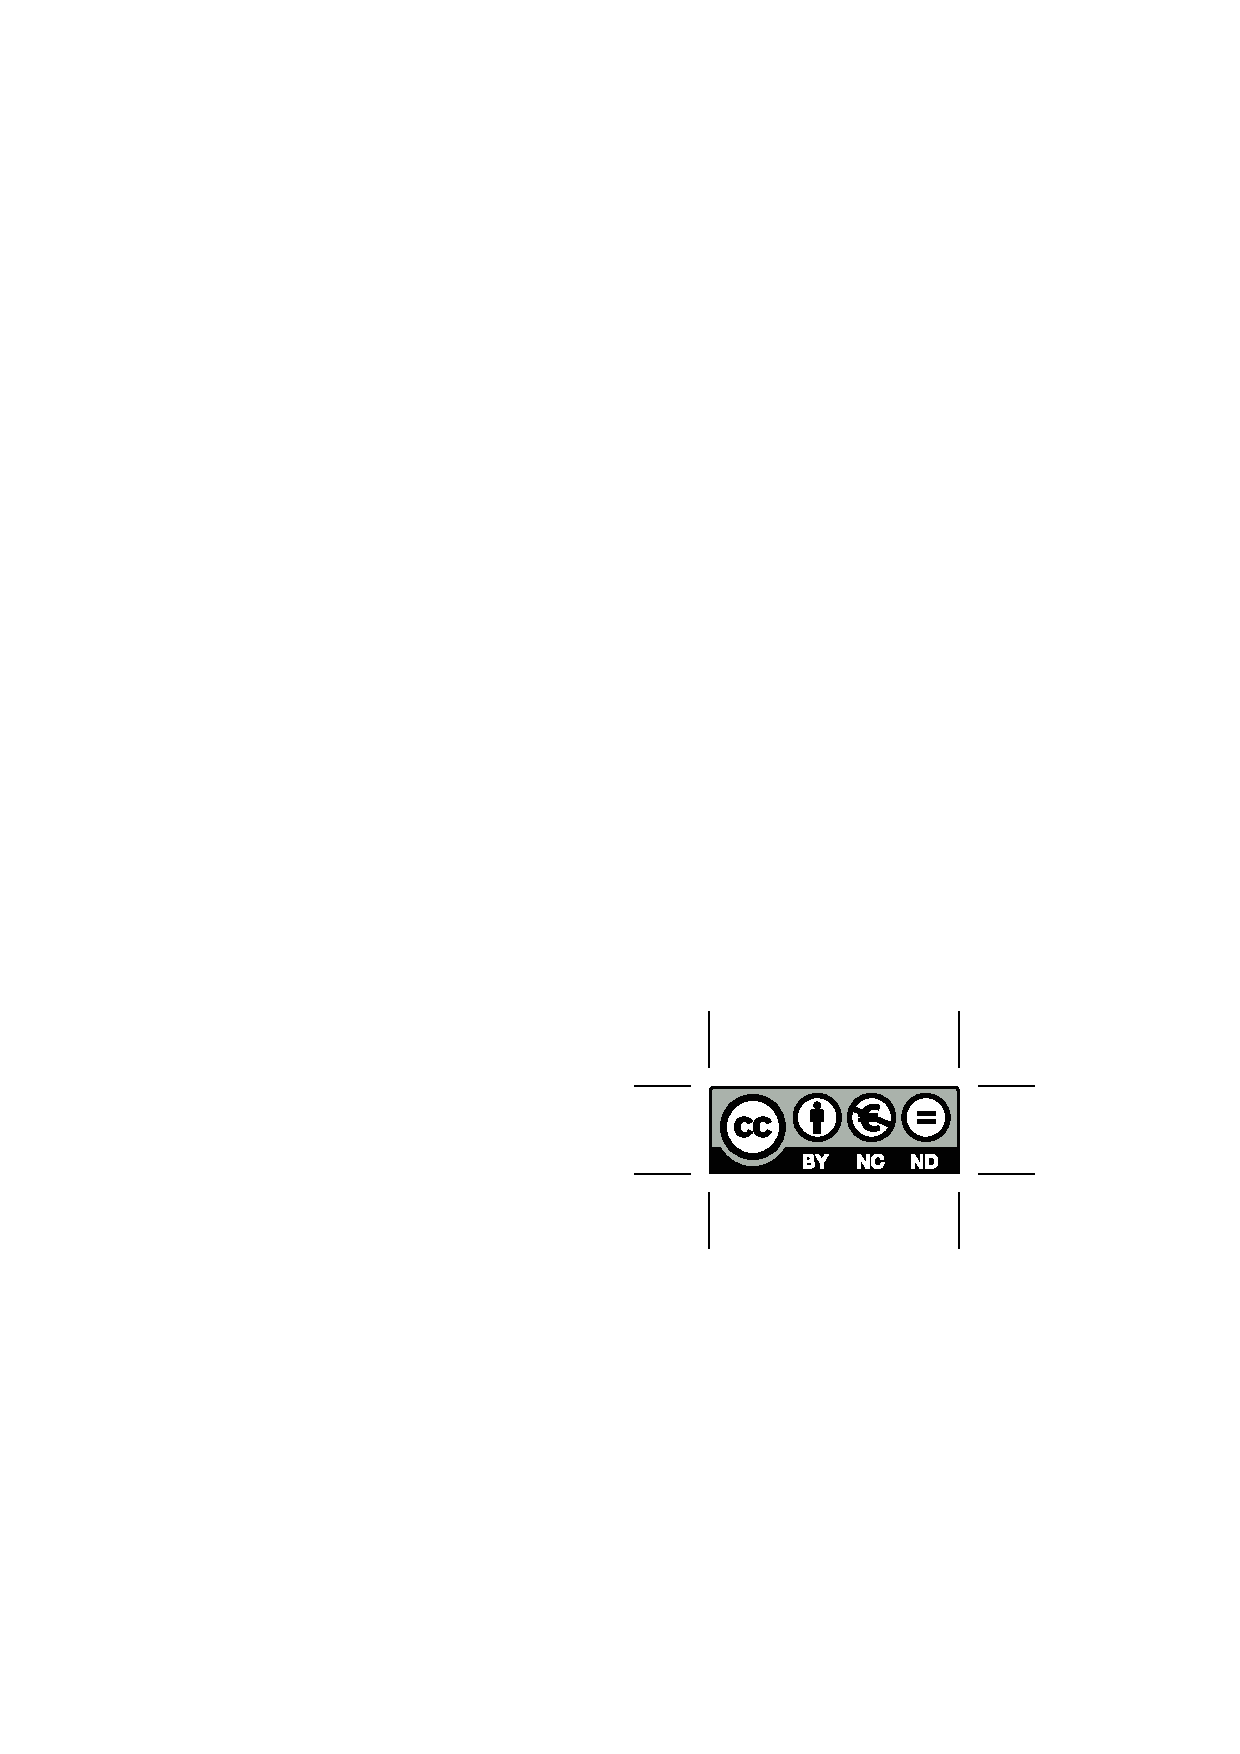
\includegraphics[height=35px]{images/by-nc-nd-eu}
	% \end{minipage}\hfill
% \end{center}
% 
% Cette \oe{}uvre est mise à disposition selon les termes de la \href{https://creativecommons.org/licenses/by-nc-nd/4.0/deed.fr}{Licence Creative Commons Attribution - Pas d’Utilisation Commerciale - Pas de Modification 4.0 International}. % consultez les conditions de la licence cc by-nc-nd, vous pouvez appliquer une licence moins restrictive, cc by-nc-sa par exemple
% 
% This project has received funding from the European Research Council
% (ERC) under the European Union’s Horizon 2020 research and innovation
% programme (grant agreement No 834238).

	% %\begin{dedication}
{\large{To my parents}}\\[5mm]
for many things to be written.
\end{dedication}
        % include a dedication.tex file
	% %\begin{acknowledgements}
These are the acknowledgements.
\end{acknowledgements}
   % include an acknowledgements.tex file
	% %% For tips on how to write a great abstract, have a look at
%%	-	https://www.cdc.gov/stdconference/2018/How-to-Write-an-Abstract_v4.pdf (presentation, start here)
%%	-	https://users.ece.cmu.edu/~koopman/essays/abstract.html
%%	-	https://search.proquest.com/docview/1417403858
%%  - 	https://www.sciencedirect.com/science/article/pii/S037837821830402X

\begin{abstract}
At the basis of the marine food chain, plankton play a key role in ocean ecology. 
Due to their daily vertical migration of several hundred meters, some of these organisms play a major role in oceanic vertical mixing.
Far from being passive, many planktonic organisms are motile and able to perceive their environment and react accordingly.

Focusing on the representative example of unidirectional migration, this thesis aims to demonstrate that these motor and sensory skills, useful for predation, are also advantageous for navigating their turbulent environment.

Limited by the measure of local variations of velocity, the inability of plankton to directly sense the flow velocity makes this navigation problem particularly challenging.
By considering non-inertial organisms swimming at constant speed and able to reorient instantaneously in response to their flow sensing, we propose a new strategy that derives from an optimal solution in a linear flow.
Taking advantage of nearby updrafts to ascend faster, this strategy is called ``surfing''.

This strategy is first characterized in various simple flows and then tested in turbulent flow simulations in which ``surfers'' are observed to migrate vertically twice as fast as simulated plankters that do not react actively to the local flow.
We then relax the assumptions of the model to demonstrate the robustness of this strategy to various plankter limitations before comparing it to various other navigation approaches, involving various optimization algorithms.
Finally we discuss of the benefit that such strategy could provide to real-life plankton and propose experimental approaches that would help finding out whether surfing is a realistic strategy for planktonic navigation before discussing the perspectives of the study.
\end{abstract}
\if@openright\cleardoublepage\else\clearpage\fi
	% %% For tips on how to write a great abstract, have a look at
%%	-	https://www.cdc.gov/stdconference/2018/How-to-Write-an-Abstract_v4.pdf (presentation, start here)
%%	-	https://users.ece.cmu.edu/~koopman/essays/abstract.html
%%	-	https://search.proquest.com/docview/1417403858
%%  - 	https://www.sciencedirect.com/science/article/pii/S037837821830402X

\begin{resumes}
Constituant la base de la chaîne alimentaire marine, le plancton joue un rôle primordial pour l’écologie océanique. De par leurs migrations verticales journalières de plusieurs centaines de mètres, certains de ces organismes participent grandement au mélange vertical océanique.
Loin d’être passifs, les planctons sont, pour beaucoup, capables de nager, de percevoir leur environnement et d’y réagir.

Au travers de l'exemple de la migration verticale, cette thèse vise à démontrer que ces capacités motrices et sensorielles, utiles à la prédation, leur donnent également un avantage pour naviguer leur environnement turbulent.

Limité par la mesure des variations locales de vitesse, et non la mesure directe de la vitesse de l'écoulement, ce problème de navigation devient particulièrement difficile. 
En considérant des organismes non inertiels nageant à vitesse constante et pouvant se réorienter instantanément en réponse à leur mesure de l'écoulement, nous proposons une nouvelle stratégie qui découle d'une solution optimale dans un écoulement linéaire. 
Permettant d'atteindre les courants ascendants à proximité pour se faire porter par l'écoulement, cette stratégie est nommée le ``surf''.

Cette stratégie est tout d'abord caractérisée grâce à des écoulements simples avant d'être testée dans des simulations d'écoulements turbulents, dans lesquels les surfeurs parviennent à migrer verticalement deux fois plus vite que des planctons ne réagissant pas à l'écoulement.
Nous démontrons la robustesse de cette stratégie de navigation aux diverses limitations auxquelles les planctons sont soumis avant de comparer  le ``surf'' à d'autres méthodes de navigation impliquant divers algorithmes d'optimisation.

Enfin nous quantifions l'avantage que pourrait procurer cette stratégie à de vrais planctons dans leur habitat turbulent et proposons des approches expérimentales qui permettraient de vérifier la capacité du plancton à surfer, avant de discuter des perspectives de cette étude.
\end{resumes}
\if@openright\cleardoublepage\else\clearpage\fi
	% \tableofcontents*\if@openright\cleardoublepage\else\clearpage\fi
	% \listoffigures*\if@openright\cleardoublepage\else\clearpage\fi
	% \listoftables*\if@openright\cleardoublepage\else\clearpage\fi
	% %%% will only print what is used ... useful.
%% also acronyms are clickable, which is awesome

\chapter*{List of Abbreviations}
\markboth{List of Abbreviations}{List of Abbreviations}
               
\begin{acronym}\itemsep-20pt\parsep-20pt %% if you remove these spacing params this list becomes huge!
\acro{ST}{Surfing on Turbulence}
\acro{NAD+}[NAD\textsuperscript{+}]{Nicotinamide Adenine Dinucleotide}
\acro{NUA}{Not Used Acronym}
\acrodefplural{BUT}{Blocks Under Test}
\end{acronym}
\if@openright\cleardoublepage\else\clearpage\fi
	% % Display as a list of symbols
\renewcommand{\nomname}{List of Symbols}
%\renewcommand{\nompreamble}{The next list describes several symbols that will be later used within the body of the document}

%% Typography:

\nomenclature[A, 1]{\(a\)}{Scalar}
\nomenclature[A, 2]{\(\vec{a},~\vec{A}\)}{Vector}
\nomenclature[A, 3]{\(\hat{\vec{a}}\)}{Unit vector}
\nomenclature[A, 4]{\(\matr{A}\)}{Matrix}
\nomenclature[A, 5]{\(\mathcal{A}\)}{Set}

%% Greek symbols

\nomenclature[B, 01]{\(\alpha\)}{Largest eigenvalue of $\GradientsSym$}
\nomenclature[B, 01]{\(\alpha_{\TimeHorizon}\)}{Dimensionless surfing time horizon defined in Eq.~\eqref{eq:tau_adapt}}
\nomenclature[B, 01]{\(\alpha_{\mathrm{swim}}\)}{Dimensionless model parameter defined in Eq.~\eqref{eq:time_horizon_model} that characterizes the importance of the swimming advection process over the viscous diffusion}
\nomenclature[B, 01]{\(\alpha_{\mathrm{meta.}}\)}{Prefactor of Kleiber's law [Eq.~\eqref{eq:kleiber}]}
\nomenclature[B, 02]{\(\beta\)}{Intermediate (or smallest in 2D) eigenvalue of $\GradientsSym$ or bearing of vehicle}
\nomenclature[B, 02]{\(\beta_{\mathrm{bear.}}\)}{Bearing, defined as the angle between a vessels orientation and the north}
\nomenclature[B, 02]{\(\beta_{\mathrm{eff.}}\)}{Efficiency of the conversion of biochemical energy to mechanic power}
\nomenclature[B, 03]{\(\gamma\)}{Smallest eigenvalue of $\GradientsSym$}
\nomenclature[B, 03]{\(\gamma_{\mathrm{sh.}}\)}{Shear rate of a simple shear flow}
\nomenclature[B, 04]{\(\delta\)}{Defined as $\delta \equiv \alpha$ when $\alpha = \beta$, characteristic value of flow stretching}
\nomenclature[B, 05]{\(\varDelta x\)}{Spatial increment}
\nomenclature[B, 06]{\(\epsilon\)}{Turbulent energy dissipation rate [Eq.~\eqref{eq:dissipation_rate}]}
\nomenclature[B, 06]{\(\epsilon_{\mathrm{learn.}}\)}{Parameter of the $\epsilon$-greedy approach that can be used in the context of a $\mathcal{Q}$ learning method [Eq.~\eqref{eq:epsilon_greedy}]}
\nomenclature[B, 07]{\(\KolmogorovScale\)}{Kolmogorov scale [Eq.~\eqref{eq:kolmogorov_scale}]}
\nomenclature[B, 08]{\(\theta\)}{Signed angle from $\Direction$ to $\SwimmingDirection$}
\nomenclature[B, 09]{\(\theta_{\gamma}\)}{Signed angle from $\Direction$ to the direction of shear}
\nomenclature[B, 10]{\(\theta_{\mathrm{\NameSurfShort}}\)}{Signed angle from $\Direction$ to $\ControlDirectionOpt$ (axis depends on the context)}
\nomenclature[B, 10]{\(\theta_{\mathrm{lat.}}\)}{Latitude}
\nomenclature[B, 10]{\(\theta_{\mathrm{dest.}}\)}{Latitude of the destination}
\nomenclature[B, 11]{\(\lambda\)}{Taylor microscale [Eq.~\eqref{eq:taylor_microscale}]}
\nomenclature[B, 11]{\(\lambda_{\mathrm{Dijk.}}\)}{Length horizon in the local Dijkstra approach}
\nomenclature[B, 11]{\(\lambda_{\mathrm{shape}}\)}{Plankter aspect ratio}
\nomenclature[B, 12]{\(\varLambda_{\mathrm{Dijk.}}\)}{Final length to reach (in the context of the application of the Dijkstra algorithm)}
\nomenclature[B, 12]{\(\varLambda_{\mathrm{shape}}\)}{Plankter shape factor that depends on the aspect ratio [Eq.~\eqref{eq:shape_factor}]}
\nomenclature[B, 13]{\(\nu\)}{Fluid kinematic viscosity}
\nomenclature[B, 14]{\(\mu\)}{Fluid dynamic viscosity}
\nomenclature[B, 15]{\(\rho_f\)}{Fluid density}
\nomenclature[B, 16]{\(\rho_p\)}{Plankter density}
\nomenclature[B, 17]{\(\sigma\)}{Standard deviation}
\nomenclature[B, 180]{\(\TimeHorizon\)}{Surfing time horizon [Eq.~\eqref{eq:surfing_optimal_swimming_direction_continuous}]}
\nomenclature[B, 181]{\(\TimeHorizon_{\Gradients}\)}{Time left before $\Gradients$ changes}
\nomenclature[B, 182]{\(\TimeHorizon_{\GradientsSym}\)}{Time left before $\GradientsSym$ changes}
\nomenclature[B, 183]{\(\TimeHorizon_{\GradientsAsym}\)}{Time left before $\GradientsAsym$ changes}
\nomenclature[B, 19]{\(\KolmogorovTimeScale\)}{Kolmogorov time scale [Eq.~\eqref{eq:kolmogorov}]}
\nomenclature[B, 20]{\(\InertialDelayRot\)}{Inertial rotation delay [Eq.~\eqref{eq:stokes_rotation}]}
\nomenclature[B, 21]{\(\ReorientationTime\)}{Reorientation time [Eq.~\eqref{eq:pedley_orientation}]}
\nomenclature[B, 22]{\(\InertialDelay\)}{Inertial delay [Eq.~\eqref{eq:stokes_motion}]}
\nomenclature[B, 23]{\(\phi_{\mathrm{long.}}\)}{Longitude}
\nomenclature[B, 23]{\(\phi_{\mathrm{dest.}}\)}{Longitude of the destination}
\nomenclature[B, 24]{\(\phi_{\Direction}\)}{Orientation of $\Direction$ with respect with the flow}
\nomenclature[B, 25]{\(\FlowVorticity\)}{Flow vorticity}
\nomenclature[B, 26]{\(\FlowVorticityScalar\)}{Flow vorticity norm}
\nomenclature[B, 27]{\(\FlowVorticityScalar_{f}\)}{Temporal pulsation}
\nomenclature[B, 28]{\(\FlowVorticityScalar_{\max}\)}{Maximal flow vorticity norm}
\nomenclature[B, 29]{\(\vec{\varOmega}\)}{Plankter angular velocity}
\nomenclature[B, 30]{\(\varOmega_{\mathrm{swim}}\)}{Plankter active angular velocity}
\nomenclature[B, 31]{\(\GradientsAsym\)}{Skew symmetric part of the flow velocity gradient tensor [Eq.~\eqref{eq:sym_def}]}

%% Letters

\nomenclature[C, 000]{\(\mathcal{A}\)}{Set of actions (reinforcement learning)}
\nomenclature[C, 001]{\(c\)}{Plankter concentration}
\nomenclature[C, 010]{\(d\)}{Plankter diameter}
\nomenclature[C, 011]{\(D\)}{Large scale flow length}
\nomenclature[C, 02]{\(\hat{\vec{e}}_{\alpha}\)}{Normalized eigenvector of $\GradientsSym$ associated to the eigenvalue $\alpha$}
\nomenclature[C, 03]{\(\hat{\vec{e}}_{\beta}\)}{Normalized eigenvector of $\GradientsSym$ associated to the eigenvalue $\beta$}
\nomenclature[C, 04]{\(\hat{\vec{e}}_{\gamma}\)}{Normalized eigenvector of $\GradientsSym$ associated to the eigenvalue $\gamma$}
\nomenclature[C, 050]{\(E\)}{Spectral energy density}
\nomenclature[C, 051]{\(E_{\mathrm{eff.}}\)}{Energetic efficiency}
\nomenclature[C, 060]{\(\mathcal{E}\)}{Total kinetic energy of the flow}
\nomenclature[C, 061]{\(\mathcal{E}_{\mathcal{G}}\)}{Set of the edges of the graph $\mathcal{G}$}
\nomenclature[C, 07]{\(\vec{f}_{\mathrm{ext.}}\)}{Resultant of external volumic forces on the fluid}
\nomenclature[C, 080]{\(\vec{F}_{\mathrm{flow}}\)}{Resultant of flow forces on the plankter}
\nomenclature[C, 085]{\(\mathcal{G}\)}{Graph}
\nomenclature[C, 09]{\(h\)}{Height of a viscous channel flow or half height of a turbulent channel flow}
\nomenclature[C, 10]{\(I(\omega_f)\)}{Module of the temporal Fourier transform of an invariant of the velocity gradient tensor, defined in Tab.\ref{tab:invariants}}
\nomenclature[C, 11]{\(k\)}{Iterator or vector number}
\nomenclature[C, 12]{\(k_{\max}\)}{Maximal vector number resolve in a simulation}
\nomenclature[C, 13]{\(l\)}{Turbulent flow length scale that ranges from $\KolmogorovScale$ to $L$}
\nomenclature[C, 13]{\(\FilterLength\)}{Filter length [Eq.~\eqref{eq:filter_length}]}
\nomenclature[C, 14]{\(L\)}{Taylor-Green vortex cell length scale or the turbulence integral scale [Eq.~\eqref{eq:integral_scale}]}
\nomenclature[C, 15]{\(\ControlDirection\)}{Preferred orientation of the plankter}
\nomenclature[C, 16]{\(\ControlDirection_{a \to b}\)}{Control to apply to get from vertex $a$ to vertex $b$ [Eq.~\eqref{eq:dijkstra_edge_direction}]}
\nomenclature[C, 17]{\(N\)}{Number of simulated plankters}
\nomenclature[C, 180]{\(m\)}{Dimension of the problem: $m=2$ for 2D and $m=3$ for 3D}
\nomenclature[C, 181]{\(M_p\)}{Plankter mass}
\nomenclature[C, 182]{\(M_{\mathrm{inert.}}\)}{Shape factor that controls the torque induced by fluid inertia [Eq.~\eqref{eq:fluid_inertia_torque}]}
\nomenclature[C, 190]{\(p\)}{Flow pressure or probability function}
\nomenclature[C, 191]{\(P_{\mathrm{tot.}}\)}{Total plankter power consumption}
\nomenclature[C, 191]{\(P_{\mathrm{swim.}}\)}{Plankter swimming power consumption}
\nomenclature[C, 191]{\(P_{\mathrm{turn}}\)}{Plankter active reorientation power consumption}
\nomenclature[C, 191]{\(P_{\mathrm{meta.}}\)}{Plankter metabolic power consumption}
\nomenclature[C, 20]{\(\SwimmingDirection\)}{Plankter orientation/swimmming direction}
\nomenclature[C, 205]{\(\mathcal{Q}\)}{Quality value function used in the context of the $\mathcal{Q}$-learning method}
\nomenclature[C, 21]{\(\TargetDirection\)}{Direction to the target}
\nomenclature[C, 21]{\(\TargetDistance\)}{Distance to the target}
\nomenclature[C, 21]{\(r_c\)}{Connectivity radius (Fig.~\ref{fig:dijkstra_edges})}
\nomenclature[C, 22]{\(\matr{R}_{\hat{\vec{x}}}(\theta)\)}{Rotation matrix of axis $\hat{\vec{x}}$ and angle $\theta$}
\nomenclature[C, 22]{\(\mathcal{R}\)}{Reward function (reinforcement learning)}
\nomenclature[C, 23]{\(\GradientsSym\)}{Symmetric part of the flow velocity gradient tensor [Eq.~\eqref{eq:sym_def}]}
\nomenclature[C, 235]{\(\mathcal{S}\)}{Set of states (reinforcement learning)}
\nomenclature[C, 24]{\(t\)}{Time}
\nomenclature[C, 25]{\(\FinalTime\)}{Final time}
\nomenclature[C, 26]{\(T_{a \to b}\)}{Edge weight corresponding to the time to get from vertex $a$ to the vertex $b$ [Eq.~\eqref{eq:dijkstra_edge_time}]}
\nomenclature[C, 27]{\(T_{L}\)}{Large-eddy turnover time}
\nomenclature[C, 27]{\(T_{\mathrm{flow}}\)}{Resultant of flow torques on the plankter}
\nomenclature[C, 27]{\(\mathcal{T}_{\mathcal{G}}\)}{Set of the target vertices of the graph $\mathcal{G}$}
\nomenclature[C, 28]{\(\FlowVelocity\)}{Flow velocity}
\nomenclature[C, 29]{\(\FlowVelocityScalar\)}{Flow velocity norm}
\nomenclature[C, 30]{\(\FlowVelocityScalar_{\max}\)}{Maximal flow velocity norm}
\nomenclature[C, 31]{\(\FlowVelocityScalar_{\mathrm{rms}}\)}{Root mean square velocity}
\nomenclature[C, 32]{\(\KolmogorovVelocityScale\)}{Kolmogorov velocity scale [Eq.~\eqref{eq:kolmogorov}]}
\nomenclature[C, 33]{\(U\)}{Large scale flow velocity}
\nomenclature[C, 35]{\(V\)}{Volume or set of graph vertices}
\nomenclature[C, 35]{\(\mathcal{V}_{\mathcal{G}}\)}{Set of the vertices of the graph $\mathcal{G}$}
\nomenclature[C, 36]{\(\Performance\)}{Effective upward velocity [Eq.~\eqref{eq:surfing_performance}]}
\nomenclature[C, 37]{\(\SwimmingVelocity\)}{Plankter swimming speed}
\nomenclature[C, 38]{\(\vec{x}\)}{Position in space}
\nomenclature[C, 39]{\(\ParticlePosition\)}{Plankter position}
\nomenclature[C, 40]{\(\Direction\)}{Target direction, vertical direction (upward)}

%% Nabla

% \nomenclature[D, 1]{\(\vec{\nabla} = \begin{pmatrix}[1.8] \displaystyle \frac{\partial}{\partial x} \\ \displaystyle \frac{\partial}{\partial y} \\ \displaystyle \frac{\partial}{\partial z} \end{pmatrix}\)}{Gradient operator}
% \nomenclature[D, 2]{\(\vec{\nabla} \cdot \FlowVelocity = \displaystyle \frac{\partial \FlowVelocityScalar_x}{\partial x} + \frac{\partial \FlowVelocityScalar_y}{\partial y} + \frac{\partial \FlowVelocityScalar_z}{\partial z}\)}{Divergence of flow velocity}
% \nomenclature[D, 3]{\(\vec{\nabla} \FlowVelocity = \begin{pmatrix}[1.8] \displaystyle \frac{\partial \FlowVelocityScalar_x}{\partial x} & \displaystyle \frac{\partial \FlowVelocityScalar_x}{\partial y} & \displaystyle \frac{\partial \FlowVelocityScalar_x}{\partial z} \\ \displaystyle \frac{\partial \FlowVelocityScalar_y}{\partial x} & \displaystyle \frac{\partial \FlowVelocityScalar_y}{\partial y} & \displaystyle \frac{\partial \FlowVelocityScalar_y}{\partial z} \\ \displaystyle \frac{\partial \FlowVelocityScalar_z}{\partial x} & \displaystyle \frac{\partial \FlowVelocityScalar_z}{\partial y} & \displaystyle \frac{\partial \FlowVelocityScalar_z}{\partial z} \end{pmatrix}\)}{Gradient tensor of flow velocity}
% \nomenclature[D, 4]{\(\vec{\nabla}^2 \FlowVelocity = \begin{pmatrix}[1.8] \displaystyle \frac{\partial^2 \FlowVelocityScalar_x}{\partial x^2} \\ \displaystyle \frac{\partial^2 \FlowVelocityScalar_y}{\partial y^2} \\ \displaystyle \frac{\partial^2 \FlowVelocityScalar_z}{\partial^2 z} \end{pmatrix}\)}{Laplacian of flow velocity}

\nomenclature[D, 1]{\(\vec{\nabla} a\)}{Gradient vector operator}
\nomenclature[D, 1]{\(\vec{\nabla} \vec{a}\)}{Gradient tensor operator}
\nomenclature[D, 2]{\(\vec{\nabla} \cdot \vec{a}\)}{Divergence operator}
\nomenclature[D, 3]{\(\vec{\nabla}^2 \vec{a}\)}{Laplacian operator}

%% Dimensionless numbers

\nomenclature[E, 1]{\(\displaystyle \mathit{Re}\)}{Reynolds number [Eq.~\eqref{eq:reynolds_number}]}
\nomenclature[E, 2]{\(\displaystyle \mathit{Re}_{\lambda}\)}{Taylor scale Reynolds number [Eq.~\eqref{eq:taylor_scale_reynolds}]}
\nomenclature[E, 3]{\(\displaystyle \mathit{Re}_p\)}{Particle Reynolds number [Eq.~\eqref{eq:particle_reynolds_number}]}
\nomenclature[E, 4]{\(\displaystyle \mathit{St}\)}{Stokes number [Eq.~\eqref{eq:stokes_number}]}

%% Subscripts and superscripts

\nomenclature[F, 1]{\(\displaystyle a_0\)}{Refers to "initial", at $t=0$ or the first term of a series}
\nomenclature[F, 2]{\(\displaystyle a_{\mathrm{\NameBhShort}}\)}{Refers to "bottom-heavy plankter"}
\nomenclature[F, 3]{\(\displaystyle a_{\mathrm{\NameSurfShort}}\)}{Refers to "surfer"}
\nomenclature[F, 4]{\(\displaystyle a^{*}\)}{Characterizes optimality}

%% Operators

\nomenclature[G, 01]{\(\displaystyle \norm{a}\)}{Absolute value for scalars}
\nomenclature[G, 02]{\(\displaystyle \norm{\vec{a}}\)}{Frobenius norm}
\nomenclature[G, 030]{\(\displaystyle \norm{\matr{A}}\)}{Frobenius norm}
\nomenclature[G, 031]{\(\displaystyle \norm{\mathcal{A}}\)}{Cardinal of a set (number of elements)}
\nomenclature[G, 04]{\(\displaystyle \frac{\partial a}{\partial t}\)}{Eulerian temporal derivative}
\nomenclature[G, 05]{\(\displaystyle \frac{D a}{D t}\)}{Particle derivative (along a flow particle trajectory)}
\nomenclature[G, 06]{\(\displaystyle \frac{d a}{d t}\)}{Derivative along a plankter trajectory}
\nomenclature[G, 07]{\(\displaystyle \exp \matr{A}\)}{Matrix exponential}
\nomenclature[G, 08]{\(\displaystyle \sgn a\)}{Sign function}
\nomenclature[G, 09]{\(\displaystyle \asym \matr{A}\)}{Skew symmetric part of a matrix}
\nomenclature[G, 10]{\(\displaystyle \sym \matr{A}\)}{Symmetric part of a matrix}
\nomenclature[G, 11]{\(\displaystyle \tr \matr{A}\)}{Matrix trace}
\nomenclature[G, 12]{\(\displaystyle \matr{A}^T\)}{Matrix transpose}
\nomenclature[G, 13]{\(\displaystyle a \equiv b\)}{Definition of $a$ as $b$}
\nomenclature[G, 14]{\(\displaystyle \left\langle a \right\rangle_N\)}{Average over $N$ simulated plankters}
\nomenclature[G, 15]{\(\displaystyle \left\langle a \right\rangle_{N, \Direction}\)}{Average over $N$ simulated plankters and over random orientations of $\Direction$}
\nomenclature[G, 16]{\(\displaystyle \vec{a}^{\bot \hat{\vec{b}}}\)}{Projection of $\vec{a}$ in the plane orthogonal to $\hat{\vec{b}}$: $\vec{a} - (\vec{a} \cdot \hat{\vec{b}}) \hat{\vec{b}}$}

\printnomenclature
\if@openright\cleardoublepage\else\clearpage\fi

%% Note: always use \input as you cannot nest \includes (amongst other things)
\pagestyle{umpage}
\floatpagestyle{umpage}
\mainmatter
	\chapter{Introduction}\label{chap:intro}

\section{What are plankton?}

The word ``plankton'' is derived from the ancient greek \textit{planktós}, that means \textit{wandering}.
This term regroups all organisms that live in water while being unfit to swim against currents.
This designation can refer to any kind of organisms in practice.
It includes many micro-organisms such as viruses, bacteria, algae, animal larvae and small crustaceans but also slowly swimming jellyfishes (Fig.~\ref{fig:marine_plankton}).
An individual organism of this group is called a plankter.
Plankton are generally separated into two groups: phytoplankton that describe the algae performing photosynthesis and zooplankton composed of animals that predate on other plankters.
\begin{figure}
	\centering
	\def\svgwidth{0.9\textwidth}
	\input{chap_intro/images/marine_plankton.pdf_tex}
  	\caption[Illustration of marine plankton.]{
  		Illustration of marine plankton. Picture of a part of the contents of a hand net. 
  		We can see a wide variety of plankters, ranging from phytoplankton (cyanobacteria, diatoms, ...) to zooplankton (copepods, dish eggs, crab larvae, worm larvae ...).
  		Adapted from \citet{nadeau2016microbial} \ccbysa ~ v4.0.
  	}
  	\label{fig:marine_plankton}
\end{figure}

\section{Why are plankton important?}

\subsection{Their role in the marine food-web}

Planktonic organisms are at the base of most of marine food-webs.
They constitute the food of many larger organisms that constitute themselves the food of even larger organisms. 
Moreover, they are the direct food source of some large mammals such as baleen whales.
Their role is then essential to sustain fisheries and marine ecology in general.

\subsection{The threat of climate change}

In a world where the climate is actively changing due to the global warming, understanding how planktonic organisms respond to it is primordial.
This necessity motivates numerous efforts to monitor plankton at a global scale \citep{brander2003use, batten2019global} and use them as a cue of the ocean ``health'' \citep{suthers2019importance}.
The climate change impacts on plankton ecology are numerous \citep{mckinnon2007vulnerability, hays2005climate}.
For instance, in addition to its direct physiological impact on plankters, water temperature influences the nutrient concentration of surface water \citep{bouman2003temperature, richardson2008hot, doney2006plankton}.
Low temperatures favour the ocean mixing that brings nutriments near the surface.
This leads to the development of large phytoplankton communities.
These conditions are particularly favourable for the development of large crustaceans.
Cold waters become then a rich environment that sustains life-dense seas.
On the contrary hotter water surface tends to stratify the upper ocean layers and prevent vertical mixing.
The absence of ocean mixing avoids sinking nutrients to get carried back to the surface.
This hinders the development of a phytoplankton communities that impact then the whole food-web.

Another consequence of climate change is the acidification of oceans. 
This is due to the growing amount of carbon dioxide released in the atmosphere that is now dissolving in the ocean.
\citet{caldeira2003anthropogenic} predict that the oceanic pH will drop by 0.3 units by 2100.
Among other effects, this acidification of the oceans especially affects organisms that rely on calcifying \citep{orr2005anthropogenic, flynn2012changes}.
This acidification causes the decrease of calcium carbonate saturation at ocean surfaces, that is needed by some plankton species (and corals) to form their external carbonate skeletons, necessary to their development.
Moreover, many plankton communities do not have the time to migrate as fast as these modifications occur.
As a consequence, some plankton species are at the verge of extinction \citep{trubovitz2020marine, lowery2020ecological}: a risk shared by all marine life that feeds on them.

\subsection{Their role on climate itself: the biological pump}

\begin{figure}
	\centering
	\def\svgwidth{0.9\textwidth}
	\input{chap_intro/schemes/biological_pump.pdf_tex}
	%\captionsetup{width=0.9\textwidth}
  	\caption[Illustration of the biological pump.]{
  		Illustration of the biological pump.
  		Adapted from \citet{ducklow2001upper}.
  		This cartoon lists the main processes of the biological pump. 
  		We focus in particular on the plankton dynamics that influence this physical process.
  		Starting from the top, carbone dioxide is dissolved into the ocean water through exchanges with the atmosphere. Inside water, CO$_2$ may react to form various carbonate species. This dissolved carbonates molecules may then be assimilated by planktonic organisms, either through photosynthesis or calcification for example. 
  		Through their movements in the flow, they actively participate to the dissemination of carbone in the water column.
  		By grazing on theme, other plankters further contribute to the transport of carbon molecules, in particular for those that perform daily vertical migrations.
  		At the same time, the excretion of zooplankton tends to aggregate with other marine debris forming larger particles called marine snow that sediment into the depth of the ocean.
  		Concentrating nutriments, this aggregates may attract hungry plankters that bring back some of the carbon molecules to the surface.
  		However the particles that reach the oceans can be trapped for huged amount of time.
  		The biological pump then contributes greatly to the global carbon trapping.
  	}
  	\label{fig:biological_pump}
\end{figure}
In addition to their impact on the marine food-web, plankton have an important role in the absorption of carbon dioxide from the atmosphere.
The plankton ecosystem acts as a ``biological pump'' that drags the carbon of the atmosphere and fix it on organic mater that sediments in the depth of the ocean.
This phenomenon entails a large variety of physical and biological processes briefly summarized here (Fig.~\ref{fig:biological_pump}).
The ocean absorbs carbon molecules through dissolution.
This phenomenon can be further enhanced by flow perturbations at the free surface, increasing air-water mixing.
The dissolved carbon molecules are then consumed by plankton species through photosynthesis but also through calcification to build outer shells and skeletons.
By grazing on them, other plankton species contribute to the vertical transport of carbon through their vertical migrations.
In addition, their excretion tend to aggregate with other ocean debris forming larger particles, called marine snow \citep{alldredge1988characteristics, turner2015zooplankton}, that settle.
During their sedimentation, these aggregates may break down due to their interactions with plankters that may feed on them.
The marine snow that makes it through and sediments in the ocean depths contributes to long term carbon trapping into solid sediments.
The oceanic flow comes into play on top of these processes.
It contributes to plankton transport and mixing, the formation of aggregates and their break up, as much as the direct advection of dissolved carbon.

The biological pump is then an essential part of the carbon cycle.
This process has led to the formation of carbon materials, such as chalk that is composed of prehistoric dead plankters \citep{farouk2020geochemical}.
More importantly, this process makes the ocean the largest carbon sink on earth \citep{lal2008carbon, hinge2020sustainability}.
The comprehension of the biological pump is then essential to model long term global climate. 
On top of that, plankton can also influence local weather.
They release organic matter in the atmosphere, such as organic sulfur molecules.
Acting as nucleation cores for water vapour, these particles eventually lead to the formation of clouds \citep{charlson1987oceanic, szyrmer1997biogenic}.
This phenomenon is particularly important when local high concentration of plankton occur, called plankton blooms \citep{behrenfeld2014resurrecting, park2017observational, creamean2019ice}.
Its impact on weather remains to be fully quantified \citep{quinn2011case} and motivates ongoing research on the topic.
For instance the Plankton, Aerosol, Cloud, ocean Ecosystem mission of the NASA \citep{werdell2019plankton} is expected to provide important satellite observations that will help understand and quantify these effects.

\section{Planktonic navigation problems}

Due to their implications in these various physical processes, modelling plankton is key to understand these important phenomena.
However modelling plankton is not trivial: (1) many plankters are motile and (2) react actively to their environment.
This motility contributes greatly to the processes described above.
Their active behavior and their responses to the environment are then key elements of plankton dynamics, that remain to be understood and accurately modelled \citep{franks2022oceanic}.
The objective of the current manuscript is to contribute to improve our understanding of the response of plankton to their flow environment. 

During their life, planktonic organisms have to face numerous survival tasks.
For instance, planktonic larvae have to disperse horizontally in the ocean to increases their chances to find a suitable settling habitat.
Plankters also have to forage for food and predate on other planktonic organisms, while having to escape their own predators.
Many zooplankton also perform diel vertical migrations: they travel to the oceans depths to avoid visual predators during the day.
Then, during the night when predators cannot see them, they get back to the ocean surface to feed on phytoplankton.
These previously described tasks involve reaching a target (either positional or directional) in a complex flow environment.
As such, these tasks can be considered as planktonic navigation problems.

It is not yet completely understood how plankters solve these problems.
Therefore navigation problems are the main interest of this study.
As we expect organisms to have evolved effective navigation strategies through natural selection, we investigate this issue using an optimality driven approach \citep{smith2011optimality}: we look for efficient navigation strategies in the context of plankton migration, in the aspiration it may lead to plankton behavior models in the future.

\subsection{How do plankton perceive their environment?}

\subsubsection{Plankton are riddled with inboard sensors!}

To address these planktonic navigation problems, the first question that arises is: how do plankters perceive their environment?
Many organisms, such as copepods [group of crustaceans sometime called the ``insects of the sea'' due to their abundance and variety \citep{schminke2007entomology}], are equipped with a primitive eye used to measure light intensity (Fig.~\ref{fig:copepod_picture}).
\begin{wrapfigure}[13]{R}[0.4\width]{0.4\textwidth}
	\vspace{-35pt}
	\centering
	\def\svgwidth{0.35\textwidth}
	\input{chap_intro/images/female_adult_acartia_clausi.pdf_tex}
	\captionsetup{width=0.35\textwidth}
  	\caption[Annotated picture of copepod]{
  		Annotated picture of copepod (Female adult \textit{Acartia Clausi}). 
  		Original picture by Minami Himemiya \ccbysa  ~ v3.0.
  	}
  	\label{fig:copepod_picture}
\end{wrapfigure}
This organ is however too underdeveloped to actually let them ``see'' their environment.
Therefore, to perceive their environment, copepods mostly rely on hair-like sensilia (sensory organs) on their antennules (antennae-shaped appendages).
Part of these sensilia are dedicated to flow measures, called setae, while others, called aesthetascs, enable chemical sensing \citep{heuschele2014chemical}.
Many planktonic larvae, such as oyster larvae, are also able to measure the direction of gravity thanks to their stotachists \citep{fuchs2015hydrodynamic}.
These organs function similarly to our internal ear that enable us to remain balanced.
Stotachists are sac-like organs containing a mobile mineralized component (statolith) that rolls in the organ when subject to acceleration or gravity (Fig.~\ref{fig:measure_vorticity}).
The statolith then triggers the setae (mechano-sensory cilia) that covers the organs internal walls.
Therefore, planktonic organisms equipped with this organ are able to measure their orientation with respect to gravity.

\subsubsection{Focus on flow sensing}\label{sec:intro_flow_sensing}

We now focus on the flow sensing of planktonic organisms. 
How does their perception of the flow differ from that of marine navigators on boats?
How does it differ from that of other animals such as flying insects, fishes or birds?

Marine navigators in charge of boat routing have access to weather forecasts and large scale ocean measures.
They can rely on this global information to plan their navigation route.
On the contrary, animals only react to the local information they can measure with their onboard sensors.
But planktonic organisms are even more limited than larger animals as they drift with the flow.
This property prevent them to directly measure the flow speed.
They are rather able to sense the difference of flow velocity between different parts of their body (gradients).

As humans, we are also subject to this phenomenon when we go swimming in the ocean.
It is easy to feel the impact of the waves and small scale currents on our body.
But if we do not visually pay enough attention to the shore, we hardly realize the large scale currents that may push us away from it.

For the readers that had the chance to take a ride in a hot air balloon, they may also have noticed they hardly felt any wind during their flight.
The only way to notice movement and apprehend the wind's presence is through the view of landscape passing below.
While flying insects, fishes and birds can assess their speed similarly using similar vision skills, most of planktonic organisms rely only on their measure of small flow perturbations (velocity gradients) due to their poor vision capabilities.
The measure of the flow speed and therefore, of their own total speed, is then out of reach.

Depending on their sensory organs, the flow information plankters have access to may be even more limited.
Even when equipped with setae (mechano-sensors) they would not be able to measure flow rotation (vorticity) as they would rotate with it as much as they drift with it.
This limits the part of the flow they can measure to pure strain (Fig.~\ref{fig:measure_strain}).
Moreover as sensing depends on the alignement of the atennules with shear, plankters orientation with respect to the flow strongly impacts sensing capabilities \citep{fields2010orientation}.
\begin{figure}
	\centering
	\begin{minipage}{0.5\textwidth}
	  	\centering
		\def\svgwidth{0.6\textwidth}
		\input{chap_turbulence/schemes/copepod_measure_strain.pdf_tex}
		\captionsetup{width=0.9\textwidth}
	  	\caption{Illustration of the measure process of the flow strain rate.}
	  	\label{fig:measure_strain}
	\end{minipage}%
	\begin{minipage}{0.5\textwidth}
		\centering
		\def\svgwidth{0.6\textwidth}
		\input{chap_turbulence/schemes/larval_measure_vorticity.pdf_tex}
		\captionsetup{width=0.9\textwidth}
	  	\caption{Illustration of the measure process of flow vorticity.}
	  	\label{fig:measure_vorticity}
	\end{minipage}
\end{figure}
If they are equipped with stotachists (gravity sensing) however, as illustrated in Fig~\ref{fig:measure_vorticity}, the flow vorticity (rotation rate of the flow) can be computed from their tilting angle with the vertical \citep{fuchs2015directional}.
Note that these organs may also let plankters react to strong flow accelerations.
Overall, when having only one or the other of these sensory organs, having access to the whole flow velocity gradients is challenging.

On the one hand, if one relies only on setae, like most copepods, one could overcome this difficulty with bottom-heaviness.
Having a heavy bottom causes immersed plankters to reorient and align with the vertical.
If the effect is strong enough, this may prevent them to rotate with the flow thus enabling them to measure flow vorticity.
However, this may limit their own active rotation capabilities.

On the other hand, if one only relies on statochists, having a non spherical shape could be helpful.
The rotation of non spherical particles is also influenced by the shear part of the flow.
However the challenge then lies in separating the part of rotation due to flow vorticity from the part due to pure strain\footnote{Note that \textbf{pure strain} (also called pure shear) is not to be confused with \textbf{simple shear} that contains a vortical part.}.

Despite these limitations, many plankton species, such as copepods, are known to use this partial flow information to detect mates, preys and predators \citep{kiorboe1999predator, kiorboe1999hydrodynamic, jiang2002hydrodynamic, kiorboe2018mechanistic}\footnote{The title of this thesis is an homage to the excellent book of \citet{kiorboe2018mechanistic}, that inspired greatly this whole study.}.
Oyster larvae are even known to be able to measure and forage underwater sounds \citep{williams2022oyster}. 
But, coming back to navigation, could plankters also use their flow sensing to travel faster towards their objective?

\subsection{Examples of planktonic navigation problems}

\begin{figure}
	\centering
	\def\svgwidth{0.9\textwidth}
	\input{chap_intro/schemes/planktonic_navigation_problems.pdf_tex}
	%\captionsetup{width=0.9\textwidth}
  	\caption{
  		Non exhaustive list and illustrations of planktonic navigation problems.
  	}
  	\label{fig:planktonic_navigation_problems}
\end{figure}
To answer this question, we need to define and formalize the planktonic navigation problem we address.
In practice a given problem depends on various parameters: the nature of the target to reach (or from which to escape), the sensory information available and the motivation to navigate.
Figure \ref{fig:planktonic_navigation_problems} lists and illustrates these different planktonic navigation problems that are described below.

\subsubsection{Close range navigation: predation and escape}

As a first example, we consider the case of prey hunting or predator escape when detection occurs thanks to local flow sensing.
The detection process controls the short range nature of the problem: from three to ten body lengths in calm water \citep{fields2010orientation}. 
This implies that hydrodynamical interactions, such as lubrification forces, need to be accounted for.
Then the behaviour of the prey or the predator also influences the problem. 
Is it possible to predict its behavior? 
Is stealth an option rather than running away?
Finally the motivation: either avoiding being eaten or feeding. 
To avoid death, the prey is motivated to react regardless of the energy used whereas the predator needs to ensure catching the prey is worth the energy consumed to catch it.

Similar navigation problems, accounting for various of the previously described effects, have already been addressed either using physics-based strategies and reinforcement learning models.
For instance, accounting for hydrodynamical interactions, \citet{zhu2022optimising} show that optimal control can be used to find the optimal navigation strategy that enables to catch a non-motile point. 
They also showed that efficient strategies can be found using reinforcement learning to catch finite-size preys and characterize the effect of the size of the prey on the navigation strategy.
\citet{borra2022reinforcement} additionally account for prey behavior and show that prey-predator systems can display complex dynamics.

However, these strategies do not account for an external flow gradient that could further modify navigation.
This is one of the aspects that could be explored in future research.
Note that from this problem also rise the questions of hydrodynamical detection strategies and hydrodynamical stealth strategies, also motivating ongoing research \citep{ren2021bluff}.

\subsubsection{Navigating to an odor source: finding a mate}

Another example consists of mate finding through chemical trails.
Particularly in the copepod group, the females of some plankton species leave a chemical trail behind as they swim \citep{weissburg1998following, bagoien2005blind, yen2010chemical}.
This odor trail is aimed to attract males that need to follow it to find their mate (phenomenon called chemotaxis).
This enables medium range sensing: up to $\approx 30$ body lengths \citep{bagoien2005blind} in quiescent water.

This complex navigation task is particularly challenging in the presence of a flow field that deforms that chemical trail.
Flow sensing can then be used to either try to find quicker path to the target but also to assess how the odor trail was deformed.
Note that tracking through chemical sensing is not exclusive to mate finding.
Experimental evidences show that odor sensing can be used by zooplankton to forage marine snow aggregates \citep{lombard2013copepods}.
The sperm cells of some marine invertebrates are also known to perform chemotaxis to reach egg cells \citep{lange2021sperm}.
On the contrary, many plankters display chemophobic responses to the detection of predator-mediated chemicals \citep{hay2009marine}.
This planktonic  navigation problem is similar, yet differs from odor tracking performed by flying insects \citep{carde2008navigational, willis2011role} due to the inability of most plankters to use visual references.

In different contexts, odor tracking has received increasing attention in the last years
These problems have been addressed using physics based models: \citet{vergassola2007infotaxis} proposes a very efficient strategy called \textit{infotaxis} to track the position of a scalar source without relying on local gradients.
The method however requires a spatial references and extensive memory.
This is relevant for complex organisms that can use spatial references using advanced vision to visualize their environment but this approach is out of reach for most plankters.
Furthermore this method does not account for flow sensing that could help to find the source.
On the contrary, \citet{lange2021sperm} proposes a simple chemotactic behavior based on gradient ascent that explains how external planktonic sperm cells find egg cells in the ocean.
Other studies rely on simple data-driven approaches. For instance \citet{koehl2007individual} deduced a simple on/off model parameterized with experiments.
This model was then used in simulations to understand how planktonic larvae increased their migration towards coral reefs in response to the chemical cues they emit.

Finally reinforcement learning methods are also a popular approach to address this problem \citep{lu2011learning, fischer2017odor, liberzon2018moth, jing2021recent, loisy2022searching, rigolli2022learning}.
Overall, reinforcement learning are shown to be a promising tool to solve this kind of navigation problems.
However most of these learning-based studies either consider simple flow environments (rather than chaotic environments such as turbulence) or consider large memory organisms with spatial reference (not applicable to the planktonic version of the problem).
Furthermore, most of these studies do not consider local flow sensing, then the question of how this information could be used to improve navigation remains to be addressed.

\subsubsection{Point to point navigation: hunting a bioluminescent target}

Yet another example of planktonic point to point navigation consists of target tracking sing basic light sensing.
The oceans contain numerous bioluminescent organisms (organisms that emit light): $76\%$ of the organisms recorded by \citet{martini2017quantification} had bioluminescent capabilities with very little variations with depth.
Despite their poor vision skills, many zooplankton react to these visual cues and trigger phototactic (attraction) or photophobic (repulsion) responses.
For instance, dinoflagellate flashing luminescence has been observed to trigger escape responses from certain species of copepods \citep{buskey1983behavioral}.
It has been suggested the dinoflagellates evolved to copy the warning signal of bioluminescent copepods to avoid being grazed \citep{buskey1985behavioral}.
On the contrary, many zooplankton species are observed to be phototactic and attracted by sunlight \citep{ringelberg1999photobehaviour}, artificial light \citep{jekely2008mechanism, krafft2021antarctic, stearns1984photosensitivity} or illuminated particles \citep{tanaka2019biased}.

Bioluminescence has an important role in marine ecology. 
It is used by marine organisms to predate, defend themselves and even to attract potential living habitats by bioluminescent bacteria  \citep{haddock2010bioluminescence}.
It also has a large impact on the carbon biological pump as bioluminescent organisms often aggregate in marine snow, then attracting organisms that feed on them.
In the context of planktonic navigation, bioluminescent organisms constitute detectable long range positional targets.

This navigation problem drawed attention in recent studies. For instance in the context of the flight of flies, \citet{fabian2018interception} showed that a proportional feedback control [called proportional navigation, also used to control the navigation of modern missiles \citep{shneydor1998missile}] can successfully model the interception of aerial targets by flies.
However no flow exploitation is considered.
Flow sensing could lead to the foraging of beneficial currents that could be used to reach (or escape) that visual target faster.
Reinforcement learning has also been shown to be a promising tool to solve this problems in simplified flow fields \citep{gunnarson2021learning} and using the information of the whole flow field \citep{biferale2019zermelo}.
However, these approaches are challenged in more complex flows such as time-dependant 3D turbulence \citep{alageshan2020machine, qiu2022active}, more representative of the complexity of plankton environment.

\subsubsection{Navigating to explore: plankton horizontal dispersion}

The population of many marine organisms is solely redistributed at their planktonic larvae stage.
As adults they fixate on surfaces preventing them to disperse anymore.
The dispersion of their larvae when a new generation births is then essential for the migration of these marine species.
While simple passive Lagrangian models are often used to model larval dispersion \citep{siegel2003lagrangian}, it has been shown that larval behavior can strongly affect the horizontal distribution of larvae \citep{naylor2006orientation, vikebo2007drift, morgan2021robotic}.
The horizontal dispersion problem consists then of a long range navigation problem where larvae need to maximize horizontal dispersion to ensure the largest settlement area is explored so the species gets the best chances of survival.

\subsubsection{Directional navigation: plankton vertical migrations}

Finally, we can consider the plankton vertical migrations.
It is yet another essential navigation problem that many plankters have to face.
The research on vertical migrations initiated two hundreds years ago when they were first observed by \citet{cuvier1817regne}.
Plankton vertical migration generally occurs either daily or seasonally \citep{bandara2021two}.

The former, called diel vertical migrations, are generally performed by grazing zooplankton that migrate to the surface during the night to graze on other plankters.\footnote{Note that all diel vertical migrations are not synchronous, and asynchronous migrations are also observed \citep{cottier2006unsynchronised}.}
Then they flee the light at dawn to avoid getting caught by visual predators (such as fishes).
These migrations are generally triggered by variations of light intensity \citep{richards1996diel, van2013diel}. 
More frequent migration can even be triggered due to cloud cover \citep{omand2021cloud}, moon light \citep{last2016moonlight} and eclipses \citep{adhikari2018effect}.

Seasonal vertical migration however, occur on much larger time scale.
Various planktonic organisms swim to the ocean depths at the beginning of winter to wait the end of the season in a dormant stage \citep{naess1991diapausing, kaartvedt1996habitat}.
The cold water of the depths keeps their metabolism slow while they wait for the time to migrate back to the surface when spring comes.
Seasonal vertical migration can also be part of larval dispersion \citep{mcmanus2012plankton, kim1994larval, vikebo2007drift}.
Some larvae may migrate near the surface to benefit from stronger currents that disperse over larger distances.

Overall vertical migration translates to a long range vertical navigation problem: Antarctic krill may migrate over one kilometer distance \citep{hamner1983behavior}, corresponding to one hundred thousand time their body length!

Overall this navigation problem shines by its simplicity: plankters just have migrate in a constant direction.
In addition, plankton vertical migration is an essential part of plankton dynamics and the biological pump.
Both of these reasons make of this problem, a good first candidate to start investigating planktonic navigation.

Note that, in different contexts, similar problems has already been addressed in the past. 
For instance solutions have been deduced in simple flows thanks to reinforcement learning \citep{colabrese2017flow, gustavsson2017finding}. 
The efficiency of reinforcement learning remains however to be demonstrated in more complex flows such as time-dependant 3D turbulence \citep{alageshan2020machine}.
Moreover the link between these navigation strategies and the modeling of plankton migration remains unclear due to the ``black box'' effect of learning methods that challenges their physical interpretation.
Therefore a physics-based approach is used in this study.

\section{Thesis structure}

Due to the essential importance of vertical migrations in plankton dynamics (and the biological pump) \citep{bianchi2013diel, archibald2019modeling}, the simplicity of the navigation problem and the lack of comparative physics-based model performing in complex flow environments, this thesis focuses on the navigation related to planktonic vertical migration.
The key question is to understand to what extent local flow information can be used to improve navigation through complex flow environments.

To address this problem, in Chap.~\ref{chap:the_surfing_strategy}, we first simplify the process of plankton vertical migrations to formalize the problem into an idealized navigation problem.
We then derive an optimal solution in linear flow, which we call the \textit{surfing strategy}, and assess its performance in simple non-linear flows.
In Chap.~\ref{chap:surfing_on_turbulence}, we introduce the physics and features of turbulence. 
We then assess the performance of the previously derived surfing strategy in turbulent environments.
In Chap.~\ref{chap:surfing_robustness}, we relax the previously made assumptions to assess how robust would the strategy remain to biological constraints.
Surfing is then compared to alternative navigation methods in Chap.~\ref{chap:navigation}.
This motivates a generalisation of the surfing strategy that can be applied with more flow information.
The surfing strategy is then discussed in the context of marine biology in Chap.~\ref{chap:bio_discussion}.
We demonstrate it to be beneficial over a wide range of plankton habitats and present potential experiments that could be performed to help verifying its relevance for actual plankters.
Finally we conclude and discuss of the various perspectives of this study in Chap.~\ref{chap:perspectives}.

% \subsection{Showing the Use of Acronyms}
% 
% In the early nineties, \acs{GSM} was deployed in many European countries. \ac{GSM} offered for the first time international roaming for mobile subscribers. The \acs{GSM}’s use of \ac{TDMA} as its communication standard was debated at length. And every now and then there are big discussion whether \ac{CDMA} should have been chosen over \ac{TDMA}.
% 
% If you want to know more about \acf{GSM}, \acf{TDMA}, \acf{CDMA} and other acronyms, just read a book about mobile communication. Just to mention it: There is another \ac{UA}, for testing.

	\chapter{The Surfing Strategy}\label{chap:the_surfing_strategy}

In this chapter, we first describe the physical model used to characterize plankter motion.
We then present formally the problem of planktonic vertical migration and derive its optimal solution in linear flows.
The resulting ``surfing'' strategy is then characterized in various linear flows before it is evaluated in simple non-linear flows.

\section{Formulating the problem}\label{sec:the_surfing_strategy_problem}

We consider a plankter in a flow.
Its task is to go as fast as possible in a target direction, which is chosen to be $\Direction$, the vertical, without loss of generality.
We model the plankter as an active particle with position $\ParticlePosition (t)$, swimming in direction $\SwimmingDirection(t)$ in a flow velocity field $\FlowVelocity (\vec{x}, t)$ of vorticity $\FlowVorticity (\vec{x}, t) = \vec{\nabla} \times \FlowVelocity$.
The first question that arises is that of the plankter model.
How can we describe the motion of a plankter?

To answer this question, we first assume the plankter to be \textbf{neutrally buoyant} (this assumption is discussed in App.~\ref{app:additional_motion}, Sec.~\ref{sec:passive_processes_inertialess_effects}).
In that case, weight and buoyancy play no part in the problem.
Applying the second Newton law, we express the plankter acceleration
\begin{equation}\label{eq:newton_motion}
	M_p \frac{d^2 \ParticlePosition}{d t^2} = \vec{F}_{\mathrm{flow}}.
\end{equation}
with $M_p$ the mass of the plankter and $\vec{F}_{\mathrm{flow}}$ the resultant force exerted by the flow on the plankter.

\begin{wrapfigure}[14]{R}[0.4\width]{0.3\textwidth}
	\vspace{-5pt}
	\centering
	\def\svgwidth{0.25\textwidth}
	\input{chap_numeric/schemes/stokes_flow.pdf_tex}
	\captionsetup{width=0.25\textwidth}
  	\caption{
  		Illustration of the Stokes flow around a spherical particle.
  	}
  	\label{fig:stokes_flow}
\end{wrapfigure}
To compute this force, we need to describe the fluid motion around the plankter.
The fluid flow, composed of a \textbf{single liquid phase}, is considered \textbf{incompressible} of constant kinematic viscosity $\nu$ and density $\rho_f$.
The flow velocity $\FlowVelocity$ and pressure $p$ of such a flow are then described by the the incompressible Navier-Stokes equations,
\begin{subequations}\label{eq:navier_stokes}
	\begin{align}
		\frac{\partial \FlowVelocity}{\partial t} + \left( \FlowVelocity \cdot \vec{\nabla} \right) \, \FlowVelocity & =
		- \frac{1}{\rho_f \vec{\nabla}} p + \nu \nabla^2 \FlowVelocity + \frac{1}{\rho_f} \vec{f}_{\mathrm{ext}}\label{eq:navier_stokes_momentum} \\
		\vec{\nabla} \cdot \FlowVelocity & = 0,\label{eq:navier_stokes_mass}
	\end{align}
\end{subequations}
where Eq.~\eqref{eq:navier_stokes_momentum} describes momentum conservation while Eq.~\eqref{eq:navier_stokes_mass} is the result of mass conservation and incompressibility.
Each term of Eq.~\eqref{eq:navier_stokes_momentum} corresponds to different physical effects. 
The term $( \FlowVelocity \cdot \vec{\nabla} ) \, \FlowVelocity$ describes flow inertia, the term $\nu \nabla^2 \FlowVelocity$ corresponds to momentum diffusion due to flow viscosity and the term $(1/\rho_f) \vec{\nabla} p$ characterizes pressure effects.
The term $\vec{f}_{\mathrm{ext}}$ may include all external forcings, due to gravity for example. % or flow boundaries.

To further simplify the problem, the plankter is assumed to be \textbf{spherical} and \textbf{small} compared to the smallest scale of the flow. %Kolmogorov scale $\KolmogorovScale \ll \PlankterSize$.
In this context, we can define the particle Reynolds number $\mathit{Re}_{p}$.
This number is the result of the ratio of the intensity of the inertial and viscous term of the Navier-Stokes momentum equation \eqref{eq:navier_stokes}, at the scale of the plankter
\begin{equation}\label{eq:particle_reynolds_number}
	\mathit{Re}_p \sim \frac{\norm{\FlowVelocity - (d\ParticlePosition/dt)} \, \PlankterSize}{\nu}
\end{equation}
with $d \ParticlePosition / dt$ the actual plankter speed and $\PlankterSize$ the plankter diameter.
The term $\FlowVelocity - (d\ParticlePosition/dt)$ denotes the slip velocity: the difference between the local flow velocity and the plankter actual velocity.

If $\mathit{Re}_p \ll 1$, the flow in the immediate proximity of the plankter can be modeled by neglecting the inertial terms of the Navier-Stokes equations [Eq~\eqref{eq:navier_stokes}].
We then obtain the Stokes equation
\begin{equation}\label{eq:stokes}
	\nu \nabla^2 \FlowVelocity = \frac{1}{\rho_f} \vec{\nabla} p - \frac{1}{\rho_f} \vec{f}_{\mathrm{plank.}},
\end{equation}
where $\vec{f}_{\mathrm{plank.}}$ denotes the volumic force exerted by the plankter on the flow.
Note that the force exerted by the flow on the plankter $\vec{F}_{\mathrm{flow}}$ matches the volume integral of the volumic force exerted by the plankter on the flow $\vec{F}_{\mathrm{flow}} = -\iiint \vec{f}_{\mathrm{plank.}} dV$.

Thanks to the spherical shape of the plankter and the linearity of Stokes equation, the nearby flow velocity can be computed analytically (illustrated in Fig.~\ref{fig:stokes_flow}).
This leads to the expression of the force exerted on the plankter \citep{stokes1851effect}
\begin{equation}\label{eq:stokes_drag}
	\vec{F}_{\mathrm{flow.}} = 3 \pi \mu \PlankterSize \left( \FlowVelocity - \frac{d\ParticlePosition}{dt} \right),
\end{equation}
with $\mu$ the dynamic viscosity of the flow.
Injecting Eq~\eqref{eq:stokes_drag} into the equation of motion [Eq~\eqref{eq:newton_motion}], we obtain
\begin{equation}\label{eq:stokes_motion}
	\frac{d^2 \ParticlePosition}{d t^2} = \frac{1}{\InertialDelay} \left[ \FlowVelocity - \frac{d\ParticlePosition}{dt} \right] \quad \text{with} \quad \InertialDelay = \frac{(\rho_p + \rho_f/2) d^2}{18 \mu},
\end{equation}
with $\rho_p = \pi d^3/(6 M_p)$ the density of the plankter, assumed to be \textbf{homogeneously distributed} in the body of the plankter.
The value $\InertialDelay$ denotes the characteristic time needed for the particle to reach a constant velocity when $\FlowVelocity$ varies in time\footnote{Strictly speaking, Eq.~\eqref{eq:stokes_motion} is only valid in a steady uniform flow. Unsteadiness and irregularities cause the apparition of other flow induced forces \citep{maxey1987motion, wang2012unsteady, more2020motion}.}.
If this time is small compared to the flow time scale ($\InertialDelay \ll \KolmogorovTimeScale$), the acceleration phase of the plankter can be neglected.
This comparison of the particle relaxation time $\InertialDelay$ and the characteristic time of flow variation (corresponding to the Kolmogorov time scale $\KolmogorovTimeScale$ in turbulent flows, defined in Eq.~\ref{eq:kolmogorov} in Chap.~\ref{chap:surfing_on_turbulence}, Sec.~\ref{sec:numeric_hit}) defines the Stokes number
\begin{equation}\label{eq:stokes_number}
	\mathit{St} = \frac{\InertialDelay}{\KolmogorovTimeScale}.
\end{equation}
This number characterizes the ability of flow particles to follow streamlines (Fig.~\ref{fig:stokes_number}).
\begin{wrapfigure}[15]{L}[0.4\width]{0.3\textwidth}
	\centering
	\vspace{5pt}
	\def\svgwidth{0.25\textwidth}
	\input{chap_numeric/schemes/stokes_number.pdf_tex}
	\captionsetup{width=0.25\textwidth}
  	\caption{
  		Illustration of the influence of the Stokes number.
  	}
  	\label{fig:stokes_number}
\end{wrapfigure}

The Stokes number $\mathit{St}$ is first considered small ($\mathit{St} \ll 1$) meaning the plankter considered is \textbf{inertialess}.
This hypothesis is relaxed and discussed in App.~\ref{app:additional_motion}, Sec.~\ref{sec:passive_processes_inertial_effects}.
Additionally plankters are also assumed to swim at \textbf{constant speed} $\SwimmingVelocity$.
Under the limit of these assumptions, the translation kinematics of plankters are reduced to
\begin{equation}\label{eq:translation}
	\frac{d \ParticlePosition}{dt} = \FlowVelocity (\ParticlePosition, t) + \SwimmingVelocity \, \SwimmingDirection,
\end{equation}
with $\FlowVelocity$ the flow velocity field and $\SwimmingDirection$ the current swimming direction of the plankter.

The swimming direction $\SwimmingDirection$ of a plankter is controlled by its rotation kinematics
\begin{equation}\label{eq:translation}
	\frac{d \SwimmingDirection}{dt} = \vec{\varOmega} \times \SwimmingDirection,
\end{equation}
with $\vec{\varOmega}$ the angular velocity of the plankter.

To model the rotation dynamics of the spherical plankter we consider, one can similarly compute the viscous torque on a sphere \citep{lamb1945hydrodynamics}
\begin{equation}\label{eq:translation}
	\vec{T}_{\mathrm{flow}} = \pi \mu d^3 \left( \frac{1}{2} \FlowVorticity - \vec{\varOmega} \right)
\end{equation}
with $\FlowVorticity$ the flow vorticity.
Using the conservation of total angular momentum, one can express the rotation motion of a spherical plankter
\begin{equation}\label{eq:stokes_rotation}
	\frac{d \vec{\varOmega}}{d t} = \frac{1}{\InertialDelayRot} \left[ \frac{1}{2} \FlowVorticity(\ParticlePosition, t) - \vec{\varOmega} \right] \quad \text{with} \quad \InertialDelayRot = \frac{\rho_p d^2}{60 \mu}.
\end{equation}
Similarly to the translation dynamics, if $\InertialDelayRot \ll \KolmogorovTimeScale$, the rotation dynamics of a passive plankter reduce to its kinematics and
\begin{equation}
	\frac{d \SwimmingDirection}{d t} = \GradientsAsym \cdot \SwimmingDirection,
\end{equation}
where $\GradientsAsym = \asym \Gradients$ is the skew symmetric part local velocity gradient tensor $\Gradients$.
Note that bold symbols denote matrices.

Then to take into account active reorientation, we use the model proposed by \citet{Pedley1992}
\begin{equation}\label{eq:pedley_orientation}
		\frac{d \SwimmingDirection}{d t}  =  
		\GradientsAsym \cdot \SwimmingDirection + \frac{1}{2 \ReorientationTime} \left[ \ControlDirection - (\ControlDirection \cdot \SwimmingDirection) \SwimmingDirection \right],
\end{equation}
with $\ControlDirection$ the preferred orientation of the plankter and $\ReorientationTime$ the active reorientation time scale.
The smaller $\ReorientationTime$, the stronger is the plankter able to reorient.
Originally designed to model bottom-heavy plankters (with $\ControlDirection_{\mathrm{\NameBhShort}} = \Direction$, and the subscript $_{\mathrm{\NameBhShort}}$ referring to bottom-heavy), this expression is the result of the balance of the viscous torque exerted by the flow and the gravity torque.
Despite its origin, this model is commonly used to model particles that reorient actively \citep{colabrese2017flow, gustavsson2017finding, lange2021sperm}.
We discuss the choice of this model in Chap.~\ref{chap:surfing_robustness}, Sec.~\ref{sec:surfing_on_turbulence_p_control}.

\begin{wrapfigure}[9]{R}[0.5\width]{0.35\textwidth}
	\centering
	\vspace{-10pt}
	\def\svgwidth{0.3\textwidth}
	\input{chap_turbulence/schemes/performance.pdf_tex}
	\captionsetup{width=0.3\textwidth}
  	\caption{Illustration of performance evaluation.}
  	\label{fig:performance_description}
\end{wrapfigure}
Assuming for now that the reorienting torque is strong enough, then $\ReorientationTime \ll \KolmogorovTimeScale$ and the plankter can be assumed to reorient instantaneously.
As a consequence, the swimming direction is always aligned with the preferred direction [$\SwimmingDirection(t) = \ControlDirection(t)$].
The complete set of equations that describe plankter motion then reads
\begin{subequations}\label{eq:surfing_motion}
	\begin{align}
		\frac{d \ParticlePosition}{dt} &= \FlowVelocity (\ParticlePosition, t) + \SwimmingVelocity \, \SwimmingDirection, \\
		\SwimmingDirection(t) &= \ControlDirection(t).
	\end{align}
\end{subequations}
This hypothesis, assumed for most of the study, is relaxed and discussed in Chap.~\ref{chap:surfing_robustness}, Sec.~\ref{sec:surfing_on_turbulence_rtime}.
% \begin{wrapfigure}[10]{R}[0.5\width]{0.35\textwidth}
	% \centering
	% \vspace{-10pt}
	% \def\svgwidth{0.3\textwidth}
	% \input{chap_turbulence/schemes/problem.pdf_tex}
	% \captionsetup{width=0.3\textwidth}
  	% \caption{Illustration of the problem.}
  	% \label{fig:problem_description}
% \end{wrapfigure}
Finally, while more general swimming behaviors could eventually be considered (cf. App.~\ref{app:energetic_cost}, Sec.~\ref{sec:on_off}), at this stage, the plankter swimming speed $\SwimmingVelocity$ is assumed \textbf{constant}.
\begin{table}
	\center
	\begin{tabular*}{\textwidth}{ l }
		\toprule
		% Figure \\
		% \midrule \\[1ex]
		{\labelitemi} $\SwimmingVelocity$ constant \\
		{\labelitemi} inertialess \\
		{\labelitemi} neutrally buoyant \\
		{\labelitemi} mass homogeneously distributed in the plankter body \\
		{\labelitemi} small compared to the smallest flow scale \\
		{\labelitemi} instantaneous reorientation ($\SwimmingDirection = \ControlDirection$) \\
		{\labelitemi} sensing limited to $\Direction$ and $\Gradients$ \\
		{\labelitemi} memoryless \\
		\bottomrule
	\end{tabular*}
	\caption{
		List of the problem assumptions.
	}
	\label{tab:problem_assumptions}
\end{table}

Concerning sensing, we assume the plankter \textbf{sense the full local flow velocity gradient tensor} $\Gradients (\ParticlePosition, t)$, simply noted $\Gradients$ below, and \textbf{the vertical direction} $\Direction$.
The plankter then responds \textbf{instantaneously} to this information by choosing a preferred direction $\ControlDirection(\Gradients,\Direction)$, \textbf{without any memory}.
All of these assumptions are summed up in Tab.~\ref{tab:problem_assumptions}.

The metric used to quantify the performance of the plankters is the effective velocity, $\Performance$ (Fig.~\ref{fig:performance_description}), defined as the long-time average velocity along $\Direction$
\begin{equation}
	\label{eq:surfing_performance}
	\Performance = \lim_{\FinalTime\to\infty} \frac{\ParticlePosition (\FinalTime) - \ParticlePosition (0)}{\FinalTime} \cdot \Direction.
\end{equation}
In the language of control theory (resp. reinforcement learning), $\ControlDirection(\Gradients,\Direction)$ is the control (resp. policy) and $\Performance$ is the objective function (resp. return).

\section{Optimal solution in linear flows: surfing}\label{sec:the_surfing_strategy_derivation}

\subsection{Derivation of the surfing strategy}\label{sec:the_surfing_strategy_derivation}

To derive the surfing strategy, we start from the equation of motion of an inertialess active particle \eqref{eq:surfing_motion}.
The fluid flow $\FlowVelocity$ at position $\ParticlePosition$ and time $t$ can be approximated using a linear approximation
\begin{equation}
	\label{eq:surfing_linear}
	\FlowVelocity (\vec{x}, t) \approx \FlowVelocity_0 + (\Gradients)_0 \cdot \left(\vec{x}  - \ParticlePosition_0\right)+ \, \left(\frac{\partial \FlowVelocity}{\partial t} \right)_0 \left( t - t_0\right)
\end{equation}
for which the $0$ subscript denotes evaluation at $t = t_0$ and $\vec{x} = \ParticlePosition_0$ [i.e. $\FlowVelocity_0 = \FlowVelocity(\ParticlePosition_0, t_0)$].
Without loss of generality, we can assume $t_0 = 0$ and $\ParticlePosition_0 = \vec{0}$ and drop the $0$ subscript in the following. 
By substituting this expression into Eq.~\eqref{eq:surfing_motion}, we obtain the linear approximation
\begin{equation}
	\label{eq:surfing_linear_motion}
	 \frac{d \ParticlePosition(t)}{d t} \approx \FlowVelocity + \Gradients \cdot \ParticlePosition(t)
	 + \, \left(\frac{\partial \FlowVelocity}{\partial t} \right) t + \SwimmingVelocity \,\ControlDirection(t).
\end{equation}

Integrating this first-order differential equation leads to the following solution for the displacement
\begin{multline}
	\label{eq:surfing_integration}
	\ParticlePosition(\FinalTime) =
	\left[ \exp \left( \FinalTime \Gradients \right) - \matr{Id} \right] \cdot (\Gradients)^{-1} \cdot \left[ \FlowVelocity \, + (\Gradients)^{-1} \cdot \left(\frac{\partial \FlowVelocity}{\partial t} \right) \, \right] \\
	- \, \FinalTime (\Gradients)^{-1} \cdot \left(\frac{\partial \FlowVelocity}{\partial t} \right)
	+ \, \SwimmingVelocity \int_{0}^{\FinalTime} \exp \left( (\FinalTime - t) \Gradients \right) \cdot\ControlDirection(t) \, dt ,
\end{multline}
with $\matr{Id}$, the identity matrix, $\FinalTime$ the final time and $\exp$ the matrix exponential\footnote{The inversibility of the gradient tensor $\Gradients$ is assumed to be able to write this solution conveniently but the gradient inversibility is not required to derive the following in practice.}.
The problem consists in finding the control $\ControlDirection$ such that the displacement along $\Direction$ at time $\FinalTime$ is maximum, that is
\begin{equation}
	\text{Find} ~ \ControlDirection ~ \text{such that} ~ \ParticlePosition(\FinalTime) \cdot \Direction ~ \text{is maximum}.
\end{equation}
Since $\ControlDirection$ only appears in the last term of Eq.~\eqref{eq:surfing_integration}, the problem reduces to
\begin{equation}
	\text{Find} ~ \ControlDirection ~ \text{such that} ~ \int_{0}^{\FinalTime} \exp \left[ (\FinalTime - t) \Gradients \right] \cdot\ControlDirection(t) \cdot \Direction \, dt ~ \text{is maximum}.
\end{equation}
This is done by maximizing the integrand, which can be conveniently rewritten
\begin{equation}
	\label{eq:surfing_inside}
	\text{Find} ~ \ControlDirection ~ \text{such that} ~ \left( \exp \left[ (\FinalTime - t) (\Gradients)^T \right] \cdot\Direction \right) \cdot \ControlDirection(t) ~ \text{is maximum}.
\end{equation}
The solution to the problem of Eq.~\eqref{eq:surfing_inside} is colinear with $\exp [ (\FinalTime - t) (\Gradients)^T ] \cdot \Direction$. 
This solution gives the surfing strategy
\begin{equation}
	\label{eq:surfing_optimal_swimming_direction}
	\ControlDirectionOpt = \frac{\ControlDirectionOptNN}{\norm{\ControlDirectionOptNN}}, \quad \text{with} \quad \ControlDirectionOptNN = \exp \left[ (\FinalTime - t) (\Gradients)^T \right] \cdot \Direction.
\end{equation}
%% This expression can be further simplified if we assume a continuous measure of flow velocity gradients, and we can set $t=0$
Defining $\TimeHorizon = \FinalTime - t$, as the duration left before performance evaluation, the surfing strategy can be formulated as follows
\begin{equation}
	\label{eq:surfing_optimal_swimming_direction_continuous}
	\ControlDirectionOpt = \frac{\ControlDirectionOptNN}{\norm{\ControlDirectionOptNN}}, \quad \text{with} \quad \ControlDirectionOptNN = \exp \left[ \TimeHorizon (\Gradients)^T \right] \cdot \Direction.
\end{equation}
Surfing is optimal in a linear flow. 
In a nonlinear flow however, we expect the linearization to break down after a finite time horizon.
This time horizon $\TimeHorizon$ then becomes a free parameter of the surfing strategy which needs to be optimized.
While there is no way to guess easily the optimal value of this time horizon $\TimeHorizon$ without more information, we expect it to crucially depend on the temporal statistics of the flow.

This analysis shows that, in the limit of a linear flow, the flow velocity gradient tensor $\Gradients$ is the only information needed to locally optimize the plankter trajectory. 
While some plankters are able to sense the local flow acceleration $\left({\partial \FlowVelocity}/{\partial t} \right)$ \citep{fuchs2015hydrodynamic,fuchs2018waves}, Eq.~\eqref{eq:surfing_optimal_swimming_direction_continuous} shows that it would not be of any direct use for the problem we consider\footnote{Note however that since acceleration and velocity gradients are correlated in flows (through the Navier-Stokes equation \ref{eq:navier_stokes}), acceleration may still provide indirect information that could be exploited.}.

\subsection{Physical interpretation of the strategy}\label{sec:the_surfing_strategy_interpretation}

The surfing strategy is mainly described by a matrix exponential [Eq.~\eqref{eq:surfing_optimal_swimming_direction_continuous}].
The matrix exponential is actually defined as a series.
The surfing strategy can then also alternatively be expressed as
\begin{equation}
	\ControlDirectionOpt = \frac{\ControlDirectionOptNN}{\norm{\ControlDirectionOptNN}}, \quad \text{with} \quad 
	\ControlDirectionOptNN = \left[ \sum_{k = 0}^{\infty} \frac{\TimeHorizon^k}{k!}  \left( \Gradients \right)^k \right]^T \cdot \Direction.
\end{equation}
The resulting surfing direction then appears as a weighted averaged over several directions corresponding to the terms of the series.
The value of the surfing time horizon $\TimeHorizon$ controls which term of the series predominates over the others.
For $\TimeHorizon = 0$, the first term of the series predominates. 
When $\TimeHorizon$ increases, the next terms of the series gain importance.

To further detail the implications of this exponential, we rewrite conveniently the first terms of the series
\begin{equation}
	\ControlDirectionOpt = \frac{\ControlDirectionOptNN}{\norm{\ControlDirectionOptNN}}, \quad \text{with} \quad 
	\ControlDirectionOptNN = \Direction + \TimeHorizon \, \vec{\nabla} \FlowVelocityScalar_z + \frac{1}{2} \TimeHorizon^2 \, \vec{\nabla} \left( \FlowVelocity \cdot \vec{\nabla} \FlowVelocityScalar_\DirectionScalar \right) + \dotsb,
\end{equation}
with $\FlowVelocityScalar_\DirectionScalar = \FlowVelocity \cdot \Direction$.
The first term of the series simply corresponds to the target direction $\Direction$ [Fig.~\ref{fig:physical_interpretation}\textbf{(a)}].
\begin{figure}%[H]
	\centering
	\def\svgwidth{\textwidth}
	\input{chap_turbulence/schemes/physical_interpretation.pdf_tex}
	\caption[Physical interpretation of the surfing strategy.]{
		Physical interpretation of the surfing strategy. The surfing strategy can be interpreted as a compromise between swimming straight to the target and an iterative gradient ascent method that forages beneficial currents based on local gradients.
	}
	\label{fig:physical_interpretation}
\end{figure}
It translates the fact that a surfer partly swims directly in the target direction.
The second term is in the direction of the gradient of the vertical velocity $\vec{\nabla} \FlowVelocityScalar_z$ [Fig.~\ref{fig:physical_interpretation}\textbf{(b)}]. 
This term corresponds to a gradient ascent of the vertical flow velocity $\FlowVelocityScalar_z$.
It characterizes the fact that surfers, seeking to get carried by the flow, also swim in the direction that leads to the nearest beneficial current, in the direction of $\vec{\nabla} ( \FlowVelocity \cdot \vec{\nabla} \FlowVelocityScalar_\DirectionScalar )$.
So to maximize vertical displacement, surfer also have to maximize displacement in the direction $\vec{\nabla} ( \FlowVelocity \cdot \vec{\nabla} \FlowVelocityScalar_\DirectionScalar )$.
And thus to do so, the next term of the series takes the form of the gradient of the velocity component in that direction [Fig.~\ref{fig:physical_interpretation}\textbf{(c)}].
Not content with the exploitation of ascending currents, given a large enough surfing time horizon $\TimeHorizon$, surfers also seek to exploit horizontal currents that would push them towards those upwellings.

Each of the next term of the series actually corresponds to the gradient of the flow velocity component in the direction of their precedent term.\footnote{This observation also leads to an alternative expression of the surfing strategy based on a recursion:
$\ControlDirectionOpt = \ControlDirectionOptNN/\norm{\ControlDirectionOptNN}$ with $\ControlDirectionOptNN = \sum_{k = 0}^{\infty} \ControlDirectionNN_{k}$, with $\ControlDirectionNN_{0} = \Direction$ and $\forall k > 0$, $\ControlDirectionNN_{k} = \frac{1}{k} \TimeHorizon [ \Gradients ]^T \cdot \ControlDirectionNN_{k-1}$.}
The tendency to lead plankters to ``surf'' local flow features gives its name to this strategy.

\subsection{Surfing in linear flows}\label{sec:the_surfing_strategy_linear}

A linear flow is defined by a velocity $\FlowVelocity_0$ at $\vec{x} = \vec{0}$ and $t = 0$, a constant acceleration $\partial \FlowVelocity / \partial t$ and a constant flow velocity gradient tensor $\Gradients$.
For the sake of simplicity, we consider \textbf{steady} linear flows in the following: $\partial \FlowVelocity / \partial t = \vec{0}$.
The steady flow velocity can then be expressed as the following:
\begin{equation}\label{eq:linear_velocity}
	\FlowVelocity(\vec{x}) = \FlowVelocity_0 + \Gradients \cdot \vec{x}.
\end{equation}
The surfing strategy [Eq.~\eqref{eq:surfing_optimal_swimming_direction_continuous}] is the exact solution of the vertical migration problem in any linear flow.
Thus, such flows already provide an interesting framework to assess the behavior of the surfing strategy.
For that purpose, we compare surfer trajectories [$\SwimmingDirection = \ControlDirectionOpt$, Eq.~\eqref{eq:surfing_optimal_swimming_direction_continuous}], to bottom-heavy swimmers trajectories, which always swim upwards ($\SwimmingDirection_{\mathrm{\NameBhShort}} = \Direction$), and to passive particle trajectories ($\SwimmingVelocity = 0$).
%\afterpage{
\begin{figure}[p]
	\centering
	\begin{tikzpicture}[
		arrow/.style={
			insert path={
				coordinate[pos=#1,sloped]  (aux-1)
				coordinate[pos=#1+\pgfkeysvalueof{/tikz/ga/length},sloped] (aux-2)
				(aux-1) edge[/tikz/ga/arrow] 
				(aux-2) %node[]{#1}
			}
		},
		marrow/.style={
			insert path={
				coordinate[pos=#1,sloped]  (aux-1)
				coordinate[pos=#1-\pgfkeysvalueof{/tikz/ga/length},sloped] (aux-2)
				(aux-1) edge[/tikz/ga/arrow] 
				(aux-2)
			}
		},
		ga/.cd,
		length/.initial=0.0001,
		arrow/.style={-stealth,black!20!white,solid,thick},
		marrow/.style={-stealth,black!20!white,solid,thick},
		]
	% plot
	\begin{axis}[
		% more
		hide axis,
		width=0.6\linewidth,
		axis equal image,
		view={0}{90},
		% x
		xmin=-4.0,
		xmax=4.0,
		%xlabel=$x$,
		xticklabel=\empty,
		% y
		ymin=-4.0,
		ymax=4.0,
		%ylabel=$y$,
		yticklabel=\empty,
		% colormap
		colormap={flow}{color=(ColorFlowLow!10!white) color=(white) color=(ColorFlowHigh!10!white)},
		point meta min=-1,
		point meta max=1,
		% shift
		xshift=-0.25\linewidth,
		% ticks
		tickwidth=0,
		% legend
		legend style={draw=none, fill=none, /tikz/every even column/.append style={column sep=4pt}, at={(1.0, 1.02)}, anchor=south},
		legend cell align=left,
		legend columns=-1,
	]
	% flow seed 0
	% \addplot3 [
		% domain=-4.0:4.0,
		% domain y=-4.0:4.0,
		% samples=50,
		% contour filled={levels={-4.0, -3.6, -3.2, -2.8, -2.4, -2.0, -1.6, -1.2, -0.8, -0.4, 0.0, 0.4, 0.8, 1.6, 2.0, 2.4, 2.8, 3.2, 3.6, 4.0}},
	% ] {-0.23877790427740347 * x * y + 0.851066605494797 * y^2 / 2.0 - -0.4020644946639108 * x^2 / 2.0 + 0.9698253216979433 * y - -0.24380083140440792 * x}; % axy + by^2/2 - cx^2/2 + u_x y - u_y x
	% \addlegendentry{$\norm{\FlowVelocity}$}
	\addplot3 [
		domain=-4.0:4.0,
		domain y=-4.0:4.0,
		samples=50,
		color=black!20!white,
		contour gnuplot={levels={-4.0, -3.6, -3.2, -2.8, -2.4, -2.0, -1.6, -1.2, -0.8, -0.4, 0.0, 0.4, 0.8, 1.6, 2.0, 2.4, 2.8, 3.2, 3.6, 4.0}, labels=false, draw color=black!20!white},
	] {-0.23877790427740347 * x * y + 0.851066605494797 * y^2 / 2.0 - -0.4020644946639108 * x^2 / 2.0 + 0.9698253216979433 * y - -0.24380083140440792 * x} % axy + by^2/2 - cx^2/2 + u_x y - u_y x
	[arrow/.list={0.0, 0.1, 0.3, 0.4, 0.5, 0.6, 0.7, 0.8}] [marrow/.list={0.9, 1.0}];
	\addlegendentry{streamlines}
	% passive
	\addplot
	[
		color=ColorPassive,
		mark=*,
		mark options={mark indices={41}},
		line width=1pt,
		mark size=0.6mm
	]
	table[
		x index=1, 
		y index=2, 
		col sep=comma, 
		comment chars=\#,
		unbounded coords=discard,
	]{chap_surfing/data/various_linear_flows/flow_linear_incompressible_parameters__seed_0__passive_trajectory.csv};
	\addlegendentry{passive}
	% bottom heavy
	\addplot
	[
		color=ColorBh,
		mark=*,
		mark options={mark indices={41}},
		line width=1pt,
		mark size=0.6mm
	]
	table[
		x index=1, 
		y index=2, 
		col sep=comma, 
		comment chars=\#,
		unbounded coords=discard,
	]{chap_surfing/data/various_linear_flows/flow_linear_incompressible_parameters__seed_0__bottom_heavy_trajectory.csv};
	\addlegendentry{\NameBhShort}
	\addplot3 [ColorBh!75!white,opacity=1.0,very thick,-stealth,quiver={
		u={0.0},
		v={1.0},
		scale arrows=0.8
		}] table[
		x index=1, 
		y index=2, 
		col sep=comma,
		comment chars=\#,
		each nth point={5},
		unbounded coords=discard,
		]{chap_surfing/data/various_linear_flows/flow_linear_incompressible_parameters__seed_0__bottom_heavy_trajectory.csv};
	\addlegendentry{$\SwimmingDirection_{\mathrm{\NameBhShort}}$}
	% surfer
	\addplot
	   [
	   color=ColorSurf,
	   mark=*,
   		mark options={mark indices={41}},
   		line width=1pt,
   		mark size=0.6mm
	   ]
	   table[
	   x index=1, 
	   y index=2, 
	   col sep=comma, 
	   comment chars=\#,
	   unbounded coords=discard,
	   ]{chap_surfing/data/various_linear_flows/flow_linear_incompressible_parameters__seed_0__surfer_trajectory.csv};
	\addlegendentry{\NameSurfShort}
	\addplot3 [ColorSurf!75!white,opacity=1.0,very thick,-stealth,quiver={
		u={\thisrowno{3}},
		v={\thisrowno{4}},
		scale arrows=0.8
		}] table[
		x index=1, 
		y index=2,
		col sep=comma,
		comment chars=\#,
		each nth point={5},
		unbounded coords=discard,
		]{chap_surfing/data/various_linear_flows/flow_linear_incompressible_parameters__seed_0__surfer_trajectory.csv};
	\addlegendentry{$\SwimmingDirection_{\mathrm{\NameSurfShort}}$}
	% start position
	\addplot[mark=*, mark size=1.2mm] coordinates {(0,0)} node[black, text opacity=1, below, pos=1, anchor=west, xshift=+0.01\linewidth]{start};
	\draw[black,->,-stealth] (axis cs:3.0,2.0) -- (axis cs:3.0,3.4) node [anchor=east, pos=0.5, text opacity=1] {$\Direction$};
	% end axis
	\end{axis}



	\begin{axis}[
		at={(0.42\linewidth, 0.0)},
		% more
		hide axis,
		width=0.6\linewidth,
		axis equal image,
		view={0}{90},
		% x
		xmin=-4.0,
		xmax=4.0,
		%xlabel=$x$,
		xticklabel=\empty,
		% y
		ymin=-4.0,
		ymax=4.0,
		%ylabel=$y$,
		yticklabel=\empty,
		% colormap
		colormap={flow}{color=(ColorFlowLow!10!white) color=(white) color=(ColorFlowHigh!10!white)},
		point meta min=-1,
		point meta max=1,
		% shift
		xshift=-0.25\linewidth,
		% ticks
		tickwidth=0,
	]
	% % flow seed 1
	% \addplot3 [
		% domain=-4.0:4.0,
		% domain y=-4.0:4.0,
		% samples=50,
		% contour filled={levels={-4.0, -3.6, -3.2, -2.8, -2.4, -2.0, -1.6, -1.2, -0.8, -0.4, 0.0, 0.4, 0.8, 1.6, 2.0, 2.4, 2.8, 3.2, 3.6, 4.0}},
	% ] {-0.6672404816206614 * x * y + -0.00721956343294607 * y^2 / 2.0 - 0.3309503849175786 * x^2 / 2.0 + -0.9360171890393105 * y - 0.3519542893941592 * x}; % axy + by^2/2 - cx^2/2 + u_x y - u_y x
	\addplot3 [
		domain=-4.0:4.0,
		domain y=-4.0:4.0,
		samples=50,
		contour gnuplot={levels={-4.0, -3.6, -3.2, -2.8, -2.4, -2.0, -1.6, -1.2, -0.8, -0.4, 0.0, 0.4, 0.8, 1.6, 2.0, 2.4, 2.8, 3.2, 3.6, 4.0}, labels=false, draw color=black!20!white},
	] {-0.6672404816206614 * x * y + -0.00721956343294607 * y^2 / 2.0 - 0.3309503849175786 * x^2 / 2.0 + -0.9360171890393105 * y - 0.3519542893941592 * x} % axy + by^2/2 - cx^2/2 + u_x y - u_y x
	[arrow/.list={0.0, 0.1, 0.3, 0.4, 0.6}] [marrow/.list={0.5, 0.8, 0.7, 0.9, 1.0}];
	% passive
	\addplot
	   [
	   color=ColorPassive,
	   mark=*,
   		mark options={mark indices={41}},
   		line width=1pt,
   		mark size=0.6mm
	   ]
	   table[
	   x index=1, 
	   y index=2, 
	   col sep=comma, 
	   comment chars=\#,
	   unbounded coords=discard,
	   ]{chap_surfing/data/various_linear_flows/flow_linear_incompressible_parameters__seed_1__passive_trajectory.csv};
	% bottom heavy
	\addplot
	   [
	   color=ColorBh,
	   mark=*,
   		mark options={mark indices={41}},
   		line width=1pt,
   		mark size=0.6mm
	   ]
	   table[
	   x index=1, 
	   y index=2, 
	   col sep=comma, 
	   comment chars=\#,
	   unbounded coords=discard,
	   ]{chap_surfing/data/various_linear_flows/flow_linear_incompressible_parameters__seed_1__bottom_heavy_trajectory.csv};
	\addplot3 [ColorBh!75!white,opacity=1.0,very thick,-stealth,quiver={
		u={0.0},
		v={1.0},
		scale arrows=0.8
		}] table[
		x index=1, 
		y index=2, 
		col sep=comma,
		comment chars=\#,
		each nth point={5},
		unbounded coords=discard,
		]{chap_surfing/data/various_linear_flows/flow_linear_incompressible_parameters__seed_1__bottom_heavy_trajectory.csv};
	% surfer
	\addplot
	   [
	   color=ColorSurf,
	   mark=*,
  		mark options={mark indices={41}},
  		line width=1pt,
  		mark size=0.6mm
	   ]
	   table[
	   x index=1, 
	   y index=2, 
	   col sep=comma, 
	   comment chars=\#,
	   unbounded coords=discard,
	   ]{chap_surfing/data/various_linear_flows/flow_linear_incompressible_parameters__seed_1__surfer_trajectory.csv};
	\addplot3 [ColorSurf!75!white,opacity=1.0,very thick,-stealth,quiver={
		u={\thisrowno{3}},
		v={\thisrowno{4}},
		scale arrows=0.8
		}] table[
		x index=1, 
		y index=2,
		col sep=comma,
		comment chars=\#,
		each nth point={5},
		unbounded coords=discard,
		]{chap_surfing/data/various_linear_flows/flow_linear_incompressible_parameters__seed_1__surfer_trajectory.csv};
	% start position
	\addplot[mark=*, mark size=1.2mm] coordinates {(0,0)} node[black, text opacity=1, below, pos=1, anchor=west, xshift=+0.01\linewidth]{start};
	\draw[black,->,-stealth] (axis cs:3.0,0.0) -- (axis cs:3.0,1.4) node [anchor=east, pos=0.5, text opacity=1] {$\Direction$};
	% end axis
	\end{axis}



	\begin{axis}[
		at={(0.0, -0.42\linewidth)},
		% more
		hide axis,
		width=0.6\linewidth,
		axis equal image,
		view={0}{90},
		% x
		xmin=-4.0,
		xmax=4.0,
		%xlabel=$x$,
		xticklabel=\empty,
		% y
		ymin=-4.0,
		ymax=4.0,
		%ylabel=$y$,
		yticklabel=\empty,
		% colormap
		colormap={flow}{color=(ColorFlowLow!10!white) color=(white) color=(ColorFlowHigh!10!white)},
		point meta min=-1,
		point meta max=1,
		% shift
		xshift=-0.25\linewidth,
		% ticks
		tickwidth=0,
	]
	% % flow seed 2
	% \addplot3 [
		% domain=-4.0:4.0,
		% domain y=-4.0:4.0,
		% samples=50,
		% contour filled={levels={-4.0, -3.6, -3.2, -2.8, -2.4, -2.0, -1.6, -1.2, -0.8, -0.4, 0.0, 0.4, 0.8, 1.6, 2.0, 2.4, 2.8, 3.2, 3.6, 4.0}},
	% ] {0.6443260129007636 * x * y + -0.40978388414900213 * y^2 / 2.0 - -0.042013646480245 * x^2 / 2.0 + -0.6516966058444201 * y - -0.7584797518265484 * x}; % axy + by^2/2 - cx^2/2 + u_x y - u_y x
	\addplot3 [
		domain=-4.0:4.0,
		domain y=-4.0:4.0,
		samples=50,
		contour gnuplot={levels={-4.0, -3.6, -3.2, -2.8, -2.4, -2.0, -1.6, -1.2, -0.8, -0.4, 0.0, 0.4, 0.8, 1.6, 2.0, 2.4, 2.8, 3.2, 3.6, 4.0}, labels=false, draw color=black!20!white},
	] {0.6443260129007636 * x * y + -0.40978388414900213 * y^2 / 2.0 - -0.042013646480245 * x^2 / 2.0 + -0.6516966058444201 * y - -0.7584797518265484 * x} % axy + by^2/2 - cx^2/2 + u_x y - u_y x
	[arrow/.list={0.4, 0.6, 0.7, 0.8, 0.9, 1.0}] [marrow/.list={0.0, 0.1, 0.2, 0.3, 0.5}];
	% passive
	\addplot
	   [
	   color=ColorPassive,
	   mark=*,
   		mark options={mark indices={41}},
   		line width=1pt,
   		mark size=0.6mm
	   ]
	   table[
	   x index=1, 
	   y index=2, 
	   col sep=comma, 
	   comment chars=\#,
	   unbounded coords=discard,
	   ]{chap_surfing/data/various_linear_flows/flow_linear_incompressible_parameters__seed_2__passive_trajectory.csv};
	% bottom heavy
	\addplot
	   [
	   color=ColorBh,
	   mark=*,
   		mark options={mark indices={41}},
   		line width=1pt,
   		mark size=0.6mm
	   ]
	   table[
	   x index=1, 
	   y index=2, 
	   col sep=comma, 
	   comment chars=\#,
	   unbounded coords=discard,
	   ]{chap_surfing/data/various_linear_flows/flow_linear_incompressible_parameters__seed_2__bottom_heavy_trajectory.csv};
	\addplot3 [ColorBh!75!white,opacity=1.0,very thick,-stealth,quiver={
		u={0.0},
		v={1.0},
		scale arrows=0.8
		}] table[
		x index=1, 
		y index=2, 
		col sep=comma,
		comment chars=\#,
		each nth point={5},
		unbounded coords=discard,
		]{chap_surfing/data/various_linear_flows/flow_linear_incompressible_parameters__seed_2__bottom_heavy_trajectory.csv};
	% surfer
	\addplot
	   [
	   color=ColorSurf,
	   mark=*,
   		mark options={mark indices={41}},
   		line width=1pt,
   		mark size=0.6mm
	   ]
	   table[
	   x index=1, 
	   y index=2, 
	   col sep=comma, 
	   comment chars=\#,
	   unbounded coords=discard,
	   ]{chap_surfing/data/various_linear_flows/flow_linear_incompressible_parameters__seed_2__surfer_trajectory.csv};
	\addplot3 [ColorSurf!75!white,opacity=1.0,very thick,-stealth,quiver={
		u={\thisrowno{3}},
		v={\thisrowno{4}},
		scale arrows=0.8
		}] table[
		x index=1, 
		y index=2,
		col sep=comma,
		comment chars=\#,
		each nth point={5},
		unbounded coords=discard,
		]{chap_surfing/data/various_linear_flows/flow_linear_incompressible_parameters__seed_2__surfer_trajectory.csv};
	% start position
	\addplot[mark=*, mark size=1.2mm] coordinates {(0,0)} node[black, text opacity=1, below, pos=1, anchor=west, xshift=+0.01\linewidth]{start};
	\draw[black,->,-stealth] (axis cs:3.0,0.0) -- (axis cs:3.0,1.4) node [anchor=east, pos=0.5, text opacity=1] {$\Direction$};
	% end axis
	\end{axis}



	\begin{axis}[
		at={(0.42\linewidth, -0.42\linewidth)},
		% more
		hide axis,
		width=0.6\linewidth,
		axis equal image,
		view={0}{90},
		% x
		xmin=-4.0,
		xmax=4.0,
		%xlabel=$x$,
		xticklabel=\empty,
		% y
		ymin=-4.0,
		ymax=4.0,
		%ylabel=$y$,
		yticklabel=\empty,
		% colormap
		colormap={flow}{color=(ColorFlowLow!10!white) color=(white) color=(ColorFlowHigh!10!white)},
		point meta min=-1,
		point meta max=1,
		% shift
		xshift=-0.25\linewidth,
		% ticks
		tickwidth=0,
	]
	% flow seed 3
	% \addplot3 [
		% domain=-4.0:4.0,
		% domain y=-4.0:4.0,
		% samples=50,
		% contour filled={levels={-4.0, -3.6, -3.2, -2.8, -2.4, -2.0, -1.6, -1.2, -0.8, -0.4, 0.0, 0.4, 0.8, 1.6, 2.0, 2.4, 2.8, 3.2, 3.6, 4.0}},
	% ] {0.027285226746810765 * x * y + -0.7023493328035814 * y^2 / 2.0 - -0.7107857958014597 * x^2 / 2.0 + -0.9914048573537874 * y - -0.1308296939357293 * x}; % axy + by^2/2 - cx^2/2 + u_x y - u_y x
	\addplot3 [
		domain=-4.0:4.0,
		domain y=-4.0:4.0,
		samples=50,
		contour gnuplot={levels={-4.0, -3.6, -3.2, -2.8, -2.4, -2.0, -1.6, -1.2, -0.8, -0.4, 0.0, 0.4, 0.8, 1.6, 2.0, 2.4, 2.8, 3.2, 3.6, 4.0}, labels=false, draw color=black!20!white},
	] {0.027285226746810765 * x * y + -0.7023493328035814 * y^2 / 2.0 - -0.7107857958014597 * x^2 / 2.0 + -0.9914048573537874 * y - -0.1308296939357293 * x} % axy + by^2/2 - cx^2/2 + u_x y - u_y x
	[arrow/.list={0.3, 0.5, 0.6, 0.7, 0.8, 0.9, 1.0}] [marrow/.list={0.0, 0.1, 0.2, 0.4}];
	% passive
	\addplot
	   [
	   color=ColorPassive,
	   mark=*,
   		mark options={mark indices={41}},
   		line width=1pt,
   		mark size=0.6mm
	   ]
	   table[
	   x index=1, 
	   y index=2, 
	   col sep=comma, 
	   comment chars=\#,
	   unbounded coords=discard,
	   ]{chap_surfing/data/various_linear_flows/flow_linear_incompressible_parameters__seed_3__passive_trajectory.csv};
	% bottom heavy
	\addplot
	   [
	   color=ColorBh,
	   mark=*,
   		mark options={mark indices={41}},
   		line width=1pt,
   		mark size=0.6mm
	   ]
	   table[
	   x index=1, 
	   y index=2, 
	   col sep=comma, 
	   comment chars=\#,
	   unbounded coords=discard,
	   ]{chap_surfing/data/various_linear_flows/flow_linear_incompressible_parameters__seed_3__bottom_heavy_trajectory.csv};
	\addplot3 [ColorBh!75!white,opacity=1.0,very thick,-stealth,quiver={
		u={0.0},
		v={1.0},
		scale arrows=0.8
		}] table[
		x index=1, 
		y index=2, 
		col sep=comma,
		comment chars=\#,
		each nth point={5},
		unbounded coords=discard,
		]{chap_surfing/data/various_linear_flows/flow_linear_incompressible_parameters__seed_3__bottom_heavy_trajectory.csv};
	% surfer
	\addplot
	   [
	   color=ColorSurf,
	   mark=*,
   		mark options={mark indices={41}},
   		line width=1pt,
   		mark size=0.6mm
	   ]
	   table[
	   x index=1, 
	   y index=2, 
	   col sep=comma, 
	   comment chars=\#,
	   unbounded coords=discard,
	   ]{chap_surfing/data/various_linear_flows/flow_linear_incompressible_parameters__seed_3__surfer_trajectory.csv};
	\addplot3 [ColorSurf!75!white,opacity=1.0,very thick,-stealth,quiver={
		u={\thisrowno{3}},
		v={\thisrowno{4}},
		scale arrows=0.8
		}] table[
		x index=1, 
		y index=2,
		col sep=comma,
		comment chars=\#,
		each nth point={5},
		unbounded coords=discard,
		]{chap_surfing/data/various_linear_flows/flow_linear_incompressible_parameters__seed_3__surfer_trajectory.csv};
	% start position
	\addplot[mark=*, mark size=1.2mm] coordinates {(0,0)} node[black, text opacity=1, below, pos=1, anchor=west, xshift=+0.01\linewidth]{start};
	\draw[black,->,-stealth] (axis cs:3.0,0.0) -- (axis cs:3.0,1.4) node [anchor=east, pos=0.5, text opacity=1] {$\Direction$};
	% end axis
	\end{axis}
	% letter
	\node[] at (-3.5, 5.9) {\textbf{(a)}};
	\node[] at (2.75, 5.9) {\textbf{(b)}};
	\node[] at (-3.5, -0.4) {\textbf{(c)}};
	\node[] at (2.75, -0.4) {\textbf{(d)}};
\end{tikzpicture}

	\caption[The surfing strategy performing in linear flows.]{
		The surfing strategy performing in linear flows.
		Comparison of simulated surfers trajectories with bottom-heavy swimmers and passive particle trajectories in various linear flows.
		Simulations parameters are provided in Tab.~\ref{tab:linear_flows_simulation_parameters}. Note that $\TimeHorizon = \FinalTime - t$ is time dependant.
	}
	\label{fig:various_linear_flows}
\end{figure}
\begin{table}[p]
	\center
	\begin{tabular}{w{c}{0.1\linewidth}w{c}{0.1\linewidth}w{c}{0.2\linewidth}w{c}{0.1\linewidth}w{c}{0.1\linewidth}w{c}{0.1\linewidth}}
		\rowcolor{ColorTabularParameters}
		Fig.~\ref{fig:various_linear_flows} & $\FlowVelocity_0$ & $\Gradients$ & $\SwimmingVelocity$ & $\ParticlePosition_0$ & $\FinalTime$ \\
		\rowcolor{ColorTabularValues}
		\textbf{(a)} & $\begin{colorpmatrix} 0.97  \\ -0.244 \end{colorpmatrix}$ & $\begin{colorpmatrix} -0.239 &  0.851 \\ -0.402 & 0.239 \end{colorpmatrix}$ & 0.5 & $\begin{colorpmatrix} 0  \\ 0 \end{colorpmatrix}$ & 6 \\
		\rowcolor{ColorTabularValues}&&&&&\\[-8pt]
		\rowcolor{ColorTabularValues}
		\textbf{(b)} & $\begin{colorpmatrix} -0.936  \\ 0.352 \end{colorpmatrix}$ & $\begin{colorpmatrix} -0.667 &  -0.007 \\ 0.331 & 0.667 \end{colorpmatrix}$ & 0.5 & $\begin{colorpmatrix} 0  \\ 0 \end{colorpmatrix}$ & 1.5 \\
		\rowcolor{ColorTabularValues}&&&&&\\[-8pt]
		\rowcolor{ColorTabularValues}
		\textbf{(c)} & $\begin{colorpmatrix} -0.652  \\ -0.758 \end{colorpmatrix}$ & $\begin{colorpmatrix} 0.644 &  -0.41 \\ -0.42 & -0.644 \end{colorpmatrix}$ & 0.5 & $\begin{colorpmatrix} 0  \\ 0 \end{colorpmatrix}$ & 2 \\
		\rowcolor{ColorTabularValues}&&&&&\\[-8pt]
		\rowcolor{ColorTabularValues}
		\textbf{(d)} & $\begin{colorpmatrix} -0.991  \\ -0.131 \end{colorpmatrix}$ & $\begin{colorpmatrix} 0.027 &  -0.702 \\ -0.711 & -0.027 \end{colorpmatrix}$ & 0.5 & $\begin{colorpmatrix} 0  \\ 0 \end{colorpmatrix}$ & 1.4 \\
	\end{tabular}
	\caption{
		Parameters of the simulations presented in Fig.~\ref{fig:various_linear_flows}.
	}
	\label{tab:linear_flows_simulation_parameters}
\end{table}
%}

Trajectories are integrated numerically using a fifth-order Runge-Kutta method \citep{dormand1980family} thanks to the \textit{scipy.integrate.solve_ivp} function of the \textit{scipy} python library \footnote{The various Python scripts used to integrate 2D trajectories are provided at \url{http://www.github.com/C0PEP0D}.}.
A description of the principle of the Runge-Kutta method is provided in App.~\ref{app:runge_kutta_method}.
Unless mentioned otherwise, all trajectories integrated in 2D flows throughout this study are performed using this same procedure (as opposed to the 3D flows introduced below).
As incompressibility is an important property of plankton flow environment, we further restrict our initial analysis to steady 2D incompressible linear flows.

Figure \ref{fig:various_linear_flows}\textbf{(a)} shows a counter intuitive solution where the surfer (red) starts by swimming downwards going around the vortex to end up in a beneficial current that propels it upwards.
Note how this strategy helps avoiding being trapped in the vortex as the bottom-heavy swimmer (blue) that ends up being propelled downwards while always swimming upwards.
This illustrates how flow information can be used to optimize navigation significantly.
However in Fig.~\ref{fig:various_linear_flows}\textbf{(b)} and Fig.~\ref{fig:various_linear_flows}\textbf{(c)}, we observe very similar trajectories for surfers and bottom-heavy swimmers.
The two cases correspond to very singular case where shear is strong compared to vorticity and the stretching direction of the flow is either almost parallel or orthogonal to the target direction $\Direction$.
However in a less singular cases where the stretching direction is neither parallel nor orthogonal to $\Direction$, the benefit of surfing is significant [Fig.~\ref{fig:various_linear_flows}\textbf{(d)}].
Yet, surfing in such a strain dominated flow remains less beneficial than surfing in vortical flow such as the one presented in Fig.~\ref{fig:various_linear_flows}\textbf{(a)}.

To better understand how linear flow characteristics can influence surfing performance, one can decompose the flow into two contributions: a symmetric one, of gradient $\GradientsSym \equiv \sym \Gradients$ and a skew symmetric one, of gradient $\GradientsAsym \equiv \asym \Gradients$, both defined as follows:
\begin{equation}\label{eq:sym_def}
	\GradientsSym \equiv \sym \Gradients = \frac{1}{2} \left[ \Gradients + (\Gradients)^T \right], \quad \GradientsAsym \equiv \asym \Gradients = \frac{1}{2} \left[ \Gradients - (\Gradients)^T \right],
\end{equation}
This decomposition is commonly used to distinguish rotating regions, $\norm{\GradientsAsym} \gg \norm{\GradientsSym}$, from strain regions, $\norm{\GradientsSym} \gg \norm{\GradientsAsym}$, of the flow (Fig.~\ref{fig:decomposition}).
The skew symmetric part of the gradient is responsible for the rotation of fluid parcels while the symmetric part describes extension and contractions axes of the flow.
Each part is known to behave differently in turbulence \citep{meneveau2011lagrangian, fang2015short}.
\begin{figure}%[H]
	\centering
	\begin{tikzpicture}[
		arrow/.style={
			insert path={
				coordinate[pos=#1,sloped]  (aux-1)
				coordinate[pos=#1+\pgfkeysvalueof{/tikz/ga/length},sloped] (aux-2)
				(aux-1) edge[/tikz/ga/arrow] 
				(aux-2) %node[]{#1}
			}
		},
		marrow/.style={
			insert path={
				coordinate[pos=#1,sloped]  (aux-1)
				coordinate[pos=#1-\pgfkeysvalueof{/tikz/ga/length},sloped] (aux-2)
				(aux-1) edge[/tikz/ga/arrow] 
				(aux-2)
			}
		},
		ga/.cd,
		length/.initial=0.0001,
		arrow/.style={-stealth,black!20!white,solid,thick},
		marrow/.style={-stealth,black!20!white,solid,thick},
		]
	% plot
	\begin{axis}[
		% more
		hide axis,
		width=0.46\linewidth,
		axis equal image,
		view={0}{90},
		% x
		xmin=-4.0,
		xmax=4.0,
		%xlabel=$x$,
		xticklabel=\empty,
		% y
		ymin=-4.0,
		ymax=4.0,
		%ylabel=$y$,
		yticklabel=\empty,
		% colormap
		colormap={flow}{color=(ColorFlowLow!10!white) color=(white) color=(ColorFlowHigh!10!white)},
		point meta min=-1,
		point meta max=1,
		% shift
		xshift=-0.25\linewidth,
		% ticks
		tickwidth=0,
	]
		% flow seed 0
		\addplot3 [
			domain=-4.0:4.0,
			domain y=-4.0:4.0,
			samples=50,
			contour gnuplot={levels={-4.0, -3.6, -3.2, -2.8, -2.4, -2.0, -1.6, -1.2, -0.8, -0.4, 0.0, 0.4, 0.8, 1.6, 2.0, 2.4, 2.8, 3.2, 3.6, 4.0}, labels=false, draw color=black!20!white},
		] {-0.23877790427740347 * x * y + 0.851066605494797 * y^2 / 2.0 - -0.4020644946639108 * x^2 / 2.0 + 0.9698253216979433 * y - -0.24380083140440792 * x} % axy + by^2/2 - cx^2/2 + u_x y - u_y x
		[arrow/.list={0.0, 0.1, 0.3, 0.4, 0.5, 0.6, 0.7, 0.8}] [marrow/.list={0.9, 1.0}];
	% end axis
	\end{axis}



	\begin{axis}[
		at={(0.32\linewidth, 0.0)},
		% more
		hide axis,
		width=0.46\linewidth,
		axis equal image,
		view={0}{90},
		% x
		xmin=-4.0,
		xmax=4.0,
		%xlabel=$x$,
		xticklabel=\empty,
		% y
		ymin=-4.0,
		ymax=4.0,
		%ylabel=$y$,
		yticklabel=\empty,
		% colormap
		colormap={flow}{color=(ColorFlowLow!10!white) color=(white) color=(ColorFlowHigh!10!white)},
		point meta min=-1,
		point meta max=1,
		% shift
		xshift=-0.25\linewidth,
		% ticks
		tickwidth=0,
	]
		% flow seed 0 skew sym
		\addplot3 [
			domain=-4.0:4.0,
			domain y=-4.0:4.0,
			samples=50,
			contour gnuplot={levels={-4.0, -3.6, -3.2, -2.8, -2.4, -2.0, -1.6, -1.2, -0.8, -0.4, 0.0, 0.4, 0.8, 1.6, 2.0, 2.4, 2.8, 3.2, 3.6, 4.0}, labels=false, draw color=black!20!white},
		] {0.0 * x * y + 0.6265655500793539 * y^2 / 2.0 - -0.6265655500793539 * x^2 / 2.0 + 0.9698253216979433 * y - -0.24380083140440792 * x} % axy + by^2/2 - cx^2/2 + u_x y - u_y x
		[arrow/.list={0.2, 0.3, 0.4, 0.5, 0.6, 0.7}] [marrow/.list={0.0, 0.1, 0.8, 0.9, 1.0}];
	\end{axis}



	\begin{axis}[
		at={(0.64\linewidth, 0.0)},
		% more
		hide axis,
		width=0.46\linewidth,
		axis equal image,
		view={0}{90},
		% x
		xmin=-4.0,
		xmax=4.0,
		%xlabel=$x$,
		xticklabel=\empty,
		% y
		ymin=-4.0,
		ymax=4.0,
		%ylabel=$y$,
		yticklabel=\empty,
		% colormap
		colormap={flow}{color=(ColorFlowLow!10!white) color=(white) color=(ColorFlowHigh!10!white)},
		point meta min=-1,
		point meta max=1,
		% shift
		xshift=-0.25\linewidth,
		% ticks
		tickwidth=0,
	]
		% flow seed 0 sym
		\addplot3 [
			domain=-4.0:4.0,
			domain y=-4.0:4.0,
			samples=50,
			contour gnuplot={levels={-4.0, -3.6, -3.2, -2.8, -2.4, -2.0, -1.6, -1.2, -0.8, -0.4, 0.0, 0.4, 0.8, 1.6, 2.0, 2.4, 2.8, 3.2, 3.6, 4.0}, labels=false, draw color=black!20!white},
		] {-0.23877790427740347 * x * y + 0.22450105541544307 * y^2 / 2.0 - 0.22450105541544307 * x^2 / 2.0 + 0.9698253216979433 * y - -0.24380083140440792 * x} % axy + by^2/2 - cx^2/2 + u_x y - u_y x
		[arrow/.list={0.6, 0.7, 0.8, 0.9, 1.0}] [marrow/.list={0.0, 0.1, 0.2, 0.3, 0.4, 0.5}];
		\draw[black,->,-stealth] (axis cs:2.7,-1.48) -- (axis cs:3.25,0.0) node [anchor=west, pos=0.5, text opacity=1] {$\hat{\vec{e}}_{\alpha}$};
		\draw[black,->,-stealth] (axis cs:2.7,-1.48) -- (axis cs:1.28,-0.93) node [anchor=north, pos=0.5, text opacity=1] {$\hat{\vec{e}}_{\beta}$};
	% end axis
	\end{axis}
	% letter
	\node[] at (0.8, 2.0) {=};
	\node[] at (5.52, 2.0) {+};
	\node[] at (-2.2, 4.0) {$\FlowVelocity = \FlowVelocity_0 + \Gradients \cdot \vec{x}$};
	\node[] at (3.0, 4.0) {$\FlowVelocity = \FlowVelocity_0 + \GradientsAsym \cdot \vec{x}$};
	\node[] at (7.6, 4.0) {$\FlowVelocity = \FlowVelocity_0 + \GradientsSym \cdot \vec{x}$};
\end{tikzpicture}

	\caption[Illustration of the decomposition of a linear flow into its skew symmetric part $\GradientsAsym$ and symmetric part $\GradientsSym$.]{
		Illustration of the decomposition of a linear flow into its skew symmetric part $\GradientsAsym$ and symmetric part $\GradientsSym$. The vectors $\hat{\vec{e}}_\alpha$ and $\hat{\vec{e}}_\beta$ corresponds to the eigenvectors of $\GradientsSym$, corresponding also to the extension and compression axes of the flow.
	}
	\label{fig:decomposition}
\end{figure}

\subsubsection{Pure strain}\label{sec:the_surfing_strategy_linear_sym}

\paragraph{2D case.}
Assuming the flow is symmetric $\Gradients = \GradientsSym$, one can write all quantities in the orthonormal basis $(\hat{\vec{e}}_{\alpha}, \hat{\vec{e}}_{\beta})$, composed of the flow velocity gradients eigenvectors\footnote{This claim is the result of Cauchy's finite-dimensional spectral theorem, \citep{hawkins1975cauchy}.}.
We choose this basis so that their respective eigenvalues are sorted in descending order: $\alpha \ge \beta$. 
Due to incompressibility, the second eigenvalue is the opposite of the first one: $\delta \equiv \alpha \ge 0$ and $\beta = -\delta$.
The direction $\hat{\vec{e}}_{\alpha}$ then represents the extension axis of the flow while $\hat{\vec{e}}_{\beta}$ represents the compression axis (Fig.~\ref{fig:decomposition}).
So in a 2D symmetric linear flow, the surfing direction, Eq.~\eqref{eq:surfing_optimal_swimming_direction_continuous}, is reduced to
\begin{equation}
	\label{eq:optimal_swimming_direction_sym}
	\ControlDirectionOpt(\TimeHorizon) = \frac{e^{\delta \TimeHorizon} \DirectionScalar_\alpha \hat{\vec{e}}_{\alpha} + e^{-\delta \TimeHorizon} \DirectionScalar_\beta \hat{\vec{e}}_{\beta}}{\sqrt{e^{2 \delta \TimeHorizon} \DirectionScalar_\alpha^2 + e^{-4 \delta \TimeHorizon} \DirectionScalar_\beta^2}}.
\end{equation}
with $\DirectionScalar_\alpha = ( \Direction \cdot \hat{\vec{e}}_{\alpha} )$ and $\DirectionScalar_\beta = ( \Direction \cdot \hat{\vec{e}}_{\beta} )$.
We note that for a large enough time horizon $\TimeHorizon \delta \gg 1$, the surfing strategy aligns with the extension axis (Fig.~\ref{fig:linear_sym_surf})
\begin{equation}
	\label{eq:optimal_swimming_direction_sym_lim}
	\lim_{\TimeHorizon \to +\infty} \ControlDirectionOpt = \frac{\DirectionScalar_{\alpha}}{\abs{\DirectionScalar_{\alpha}}} \vec{e_{\alpha}} = \sgn(\DirectionScalar_{\alpha}) \, \hat{\vec{e}}_{\alpha}.
\end{equation}
As a consequence, in a symmetric linear flow, the optimal swimming direction is a balance between the target direction $\Direction$ and the stretching direction of the flow $\sgn(\DirectionScalar_{\alpha}) \, \hat{\vec{e}}_{\alpha}$. 
This alignment is controlled by the time horizon $\TimeHorizon$.
\afterpage{
\begin{figure}
	\centering
	\begin{tikzpicture}[
		arrow/.style={
			insert path={
				coordinate[pos=#1,sloped]  (aux-1)
				coordinate[pos=#1+\pgfkeysvalueof{/tikz/ga/length},sloped] (aux-2)
				(aux-1) edge[/tikz/ga/arrow] 
				(aux-2) %node[] {#1}
			}
		},
		marrow/.style={
			insert path={
				coordinate[pos=#1,sloped]  (aux-1)
				coordinate[pos=#1-\pgfkeysvalueof{/tikz/ga/length},sloped] (aux-2)
				(aux-1) edge[/tikz/ga/arrow] 
				(aux-2)
			}
		},
		ga/.cd,
		length/.initial=0.0001,
		arrow/.style={-stealth,solid,black!20!white,thick},
		marrow/.style={-stealth,solid,black!20!white,thick},
		]
	% plot
	\begin{axis}[
		% more
		hide axis,
		width=0.6\linewidth,
		axis equal image,
		view={0}{90},
		% x
		xmin=-6.0,
		xmax=2.0,
		%xlabel=$x$,
		xticklabel=\empty,
		% y
		ymin=-2.0,
		ymax=6.0,
		%ylabel=$y$,
		yticklabel=\empty,
		% colormap
		colormap={flow}{color=(ColorFlowLow!10!white) color=(white) color=(ColorFlowHigh!10!white)},
		point meta min=-1,
		point meta max=1,
		% shift
		xshift=-0.25\linewidth,
		% ticks
		tickwidth=0,
		% % legend
		% legend style={draw=none, fill=none, /tikz/every even column/.append style={column sep=4pt}, at={(1.0, 1.02)}, anchor=south},
		% legend cell align=left,
		% legend columns=-1,
	]
	\node[anchor=north east] at (axis cs:2.0, 6.0) {\textbf{(a)}};
	% flow seed 3
	% \addplot3 [
		% domain=-6.0:2.0,
		% domain y=-2.0:6.0,
		% samples=50,
		% contour filled={levels={-4.0, -3.6, -3.2, -2.8, -2.4, -2.0, -1.6, -1.2, -0.8, -0.4, 0.0, 0.4, 0.8, 1.6, 2.0, 2.4, 2.8, 3.2, 3.6, 4.0}},
	% ] {0.027285712258823203 * x * y + -0.706580136931777 * y^2 / 2.0 - -0.706580136931777 * x^2 / 2.0 + 0.0 * y - 0.0 * x}; % axy + by^2/2 - cx^2/2 + u_x y - u_y x
	\addplot3 [
		domain=-6.0:2.0,
		domain y=-2.0:6.0,
		samples=50,
		contour gnuplot={levels={-4.0, -3.6, -3.2, -2.8, -2.4, -2.0, -1.6, -1.2, -0.8, -0.4, 0.0, 0.4, 0.8, 1.6, 2.0, 2.4, 2.8, 3.2, 3.6, 4.0}, labels=false, draw color=black!20!white},
	] {0.027285712258823203 * x * y + -0.706580136931777 * y^2 / 2.0 - -0.706580136931777 * x^2 / 2.0 + 0.0 * y - 0.0 * x} % axy + by^2/2 - cx^2/2 + u_x y - u_y x
	[arrow/.list={0.3}] [marrow/.list={0.0, 0.1, 0.2, 0.4, 0.5, 0.6, 0.7, 0.8, 0.9, 1.0}];
	% time 1.0
	\addplot
		[
		color=ColorSurf!0!ColorDuration,
		mark=*,
		mark options={mark indices={41}},
		%mark repeat=10,
		%mark phase=9,
		line width=1pt,
		mark size=0.6mm
		]
		table[
		x index=1, 
		y index=2, 
		col sep=comma, 
		comment chars=\#,
		unbounded coords=discard,
		]{chap_surfing/data/linear_sym_flow/flow_symmetric_linear_incompressible_parameters__seed_3__final_time_1o0__surfer_trajectory.csv} node[pos=1, anchor=west]{$\FinalTime \delta = 1$};
	\addplot3 [ColorSurf!0!ColorDuration,opacity=1.0,very thick,-stealth,quiver={
		u={\thisrowno{3}},
		v={\thisrowno{4}},
		scale arrows=0.8
		}] table[
		x index=1, 
		y index=2,
		col sep=comma,
		comment chars=\#,
		each nth point={20},
		unbounded coords=discard,
		]{chap_surfing/data/linear_sym_flow/flow_symmetric_linear_incompressible_parameters__seed_3__final_time_1o0__surfer_trajectory.csv};
	% time 3.0
	\addplot
		[
		color=ColorSurf!50!ColorDuration,
		mark=*,
		mark options={mark indices={41}},
		line width=1pt,
		mark size=0.6mm
		]
		table[
		x index=1, 
		y index=2, 
		col sep=comma, 
		comment chars=\#,
		unbounded coords=discard,
		]{chap_surfing/data/linear_sym_flow/flow_symmetric_linear_incompressible_parameters__seed_3__final_time_3o0__surfer_trajectory.csv} node[pos=1, anchor=south west, xshift=+4pt]{$\FinalTime \delta = 3$};
	\addplot3 [ColorSurf!50!ColorDuration,opacity=1.0,very thick,-stealth,quiver={
		u={\thisrowno{3}},
		v={\thisrowno{4}},
		scale arrows=0.8
		}] table[
		x index=1, 
		y index=2,
		col sep=comma,
		comment chars=\#,
		each nth point={10},
		unbounded coords=discard,
		]{chap_surfing/data/linear_sym_flow/flow_symmetric_linear_incompressible_parameters__seed_3__final_time_3o0__surfer_trajectory.csv};
	% time 5.0
	\addplot
		[
		color=ColorSurf!100!ColorDuration,
		mark=*,
		mark options={mark indices={41}},
		line width=1pt,
		mark size=0.6mm
		]
		table[
		x index=1, 
		y index=2, 
		col sep=comma, 
		comment chars=\#,
		unbounded coords=discard,
		]{chap_surfing/data/linear_sym_flow/flow_symmetric_linear_incompressible_parameters__seed_3__final_time_5o0__surfer_trajectory.csv} node[pos=0.75, anchor=north east, xshift=+4pt]{$\FinalTime \delta = 5$};
	\addplot3 [ColorSurf!100!ColorDuration,opacity=1.0,very thick,-stealth,quiver={
		u={\thisrowno{3}},
		v={\thisrowno{4}},
		scale arrows=0.8
		}] table[
		x index=1, 
		y index=2,
		col sep=comma,
		comment chars=\#,
		each nth point={10},
		unbounded coords=discard,
		]{chap_surfing/data/linear_sym_flow/flow_symmetric_linear_incompressible_parameters__seed_3__final_time_5o0__surfer_trajectory.csv};

	% start position
	\addplot[mark=*, mark size=1.2mm] coordinates {(0,0)} node[black, text opacity=1, below, pos=1, anchor=west, xshift=+0.01\linewidth]{start};
	\draw[black,->,-stealth] (axis cs:-4.5,0.0) -- (axis cs:-4.5,1.4) node [anchor=east, pos=0.5, text opacity=1] {$\Direction$};
	% end axis
	\end{axis}



	\begin{axis}[
		at={(0.42\linewidth, 0.0)},
		% more
		hide axis,
		width=0.6\linewidth,
		axis equal image,
		view={0}{90},
		% x
		xmin=-6.0,
		xmax=2.0,
		%xlabel=$x$,
		xticklabel=\empty,
		% y
		ymin=-2.0,
		ymax=6.0,
		%ylabel=$y$,
		yticklabel=\empty,
		% colormap
		colormap={flow}{color=(ColorFlowLow!10!white) color=(white) color=(ColorFlowHigh!10!white)},
		point meta min=-1,
		point meta max=1,
		% shift
		xshift=-0.25\linewidth,
		% ticks
		tickwidth=0,
	]
	\node[anchor=north east] at (axis cs:2.0, 6.0) {\textbf{(b)}};
	% flow seed 3
	% \addplot3 [
		% domain=-6.0:2.0,
		% domain y=-2.0:6.0,
		% samples=50,
		% contour filled={levels={-4.0, -3.6, -3.2, -2.8, -2.4, -2.0, -1.6, -1.2, -0.8, -0.4, 0.0, 0.4, 0.8, 1.6, 2.0, 2.4, 2.8, 3.2, 3.6, 4.0}},
	% ] {0.027285712258823203 * x * y + -0.706580136931777 * y^2 / 2.0 - -0.706580136931777 * x^2 / 2.0 + 0.0 * y - 0.0 * x}; % axy + by^2/2 - cx^2/2 + u_x y - u_y x
	\addplot3 [
		domain=-6.0:2.0,
		domain y=-2.0:6.0,
		samples=50,
		contour gnuplot={levels={-4.0, -3.6, -3.2, -2.8, -2.4, -2.0, -1.6, -1.2, -0.8, -0.4, 0.0, 0.4, 0.8, 1.6, 2.0, 2.4, 2.8, 3.2, 3.6, 4.0}, labels=false, draw color=black!20!white},
	] {0.027285712258823203 * x * y + -0.706580136931777 * y^2 / 2.0 - -0.706580136931777 * x^2 / 2.0 + 0.0 * y - 0.0 * x} % axy + by^2/2 - cx^2/2 + u_x y - u_y x
	[arrow/.list={0.3}] [marrow/.list={0.0, 0.1, 0.2, 0.4, 0.5, 0.6, 0.7, 0.8, 0.9, 1.0}];
		% values of tau
		\draw[ColorSurf!00!ColorDuration,->,-stealth] (axis cs:0.0,0.0) -- (axis cs:0.0,3.0) node [anchor=south west, pos=1.0, text opacity=1] {$\TimeHorizon \delta = 0$};
		\draw[ColorSurf!25!ColorDuration,->,-stealth] (axis cs:0.0,0.0) -- (axis cs:3*-4.254774060615878484e-01,3*9.049690474989201538e-01) node [anchor=south, pos=1.0, text opacity=1] {$\TimeHorizon \delta = 1$};
		\draw[ColorSurf!50!ColorDuration,->,-stealth] (axis cs:0.0,0.0) -- (axis cs:3*-6.838279814833314596e-01,3*7.362111650687902520e-01) node [anchor=south east, pos=1.0, text opacity=1] {$\TimeHorizon \delta = 3$};
		\draw[ColorSurf!75!ColorDuration,->,-stealth] (axis cs:0.0,0.0) -- (axis cs:3*-7.157474507291334831e-01,3*6.983592104173514947e-01) node [anchor=east, pos=1.0, text opacity=1] {$\TimeHorizon \delta = 5$};
		\draw[ColorSurf!100!ColorDuration,->,-stealth] (axis cs:0.0,0.0) -- (axis cs:3*-7.157474507291334831e-01,3*6.983592104173514947e-01) node [anchor=north east, pos=0.8, text opacity=1] {$\TimeHorizon \delta = \infty$};
		\draw[->,-stealth,ColorSurf] (axis cs:0.0,3*0.6) arc
		[
			start angle=90,
			end angle=135,
			x radius=3*0.6,
			y radius=3*0.6
		];
		% more
		\draw[black,->,-stealth] (axis cs:-4.5,0.0) -- (axis cs:-4.5,1.4) node [anchor=east, pos=0.5, text opacity=1] {$\Direction$};
		\draw[ColorSurf!00!ColorDuration,->,-stealth] (axis cs:0.0,0.0) -- (axis cs:0.0,3.0) node [anchor=west, pos=0.5, text opacity=1] {$\ControlDirection$};
	\end{axis}
\end{tikzpicture}

	\caption[In a pure strain flow, the surfing direction tends to align with the extension axis.]{
		In a pure strain flow, the surfing direction tends to align with the extension axis.
		Influence of the time horizon $\TimeHorizon$ on the surfing strategy in a pure strain flow.
		\textbf{(a)} Comparison of surfers trajectories for various final times $\FinalTime$.
		\textbf{(b)} Surfing direction as a function of the surfing time horizon $\TimeHorizon$.
		Simulations parameters are provided in Tab.~\ref{tab:linear_sym_simulation_parameters}.
		For reference, the bottom-heavy case is evaluated for $\FinalTime \delta = 5$.
	}
	\label{fig:linear_sym_surf}
\end{figure}
\begin{table}
	\center
	\begin{tabular}{w{c}{0.12\linewidth}w{c}{0.12\linewidth}w{c}{0.24\linewidth}w{c}{0.12\linewidth}w{c}{0.12\linewidth}}
		\rowcolor{ColorTabularParameters}
		Fig. & $\FlowVelocity_0$ & $\Gradients$ & $\SwimmingVelocity$ & $\ParticlePosition_0$ \\
		\rowcolor{ColorTabularValues}
		\ref{fig:linear_sym_surf} & $\begin{colorpmatrix} 0  \\ 0 \end{colorpmatrix}$ & $\begin{colorpmatrix} 0.0273 &  -0.707 \\ -0.707 & -0.0273 \end{colorpmatrix}$ & 0.5 & $\begin{colorpmatrix} 0  \\ 0 \end{colorpmatrix}$ \\
	\end{tabular}
	\caption{
		Simulations parameters in arbitrary units of the navigation simulation presented in Fig.~\ref{fig:linear_sym_surf}.
	}
	\label{tab:linear_sym_simulation_parameters}
\end{table}
}

As illustrated in Fig.~\ref{fig:linear_sym_surf}\textbf{(b)}, for small values of the time horizon $\TimeHorizon$, the optimal direction is $\Direction$. 
As $\TimeHorizon$ increases the surfing direction tends to align with the stretching axis $\sgn(\DirectionScalar_{\alpha}) \, \hat{\vec{e}}_{\alpha}$.
Furthermore, note that the surfing direction $\ControlDirection$ converges exponentially to this limit making it almost independent of $\TimeHorizon$ for large enough vales of $\TimeHorizon \delta$.

\paragraph{3D case.}
In 3D, one can still consider the orthonormal basis of the velocity gradient composed of the flow velocity gradients eigenvectors $(\hat{\vec{e}}_{\alpha}, \hat{\vec{e}}_{\beta}, \hat{\vec{e}}_{\gamma})$, and its respective eigenvalues so that $\alpha \ge \beta \ge \gamma$.
If $\alpha > \beta$, as for the 2D case, the surfing direction tends to align with the maximal extension axis
\begin{equation}
	\label{eq:optimal_swimming_direction_sym_lim}
	\lim_{\TimeHorizon \to +\infty} \ControlDirectionOpt = \frac{\DirectionScalar_{\alpha}}{\abs{\DirectionScalar_{\alpha}}} \vec{e_{\alpha}} = \sgn(\DirectionScalar_{\alpha}) \, \hat{\vec{e}}_{\alpha}.
\end{equation}
In the singular case where $\alpha = \beta$, the surfing strategy tends towards the direction $\Direction$ projected on the stretching plane
\begin{equation}
	\label{eq:optimal_swimming_direction_sym_lim_3D}
	\lim_{\TimeHorizon \to +\infty} \ControlDirectionOpt = \frac{\Direction - \hat{\vec{e}}_{\gamma}}{\abs{\Direction - \hat{\vec{e}}_{\gamma}}}.
\end{equation}

Overall surfers essentially exploit the symmetric part of the velocity gradients by swimming in the direction of maximal stretching $\sgn(\DirectionScalar_{\alpha}) \, \hat{\vec{e}}_{\alpha}$.
While bottom-heavy swimmers still end up being pushed along the upward stretching direction, surfers, by swimming actively in that direction, maximize their displacement along the stretching axis, thus maximizing the upward velocity they can extract from flow stretching. 

\subsubsection{Vortex}\label{sec:the_surfing_strategy_linear_skew_sym}

\afterpage{
\begin{figure}
	\centering
	\begin{tikzpicture}[
		arrow/.style={
			insert path={
				coordinate[pos=#1,sloped]  (aux-1)
				coordinate[pos=#1+\pgfkeysvalueof{/tikz/ga/length},sloped] (aux-2)
				(aux-1) edge[/tikz/ga/arrow] 
				(aux-2) %node[] {#1}
			}
		},
		marrow/.style={
			insert path={
				coordinate[pos=#1,sloped]  (aux-1)
				coordinate[pos=#1-\pgfkeysvalueof{/tikz/ga/length},sloped] (aux-2)
				(aux-1) edge[/tikz/ga/arrow] 
				(aux-2)
			}
		},
		ga/.cd,
		length/.initial=0.0001,
		arrow/.style={-stealth,black!20!white,solid,thick},
		marrow/.style={-stealth,black!20!white,solid,thick},
		]
	% plot
	\begin{axis}[
		% more
		hide axis,
		width=0.6\linewidth,
		axis equal image,
		view={0}{90},
		% x
		xmin=-4.0,
		xmax=4.0,
		%xlabel=$x$,
		xticklabel=\empty,
		% y
		ymin=-2.0,
		ymax=6.0,
		%ylabel=$y$,
		yticklabel=\empty,
		% colormap
		colormap={flow}{color=(ColorFlowLow!10!white) color=(white) color=(ColorFlowHigh!10!white)},
		point meta min=-1,
		point meta max=1,
		% shift
		xshift=-0.25\linewidth,
		% ticks
		tickwidth=0,
	]
	\node[anchor=north east] at (axis cs:4.0, 6.0) {\textbf{(a)}};
	% flow seed 3
	% \addplot3 [
		% domain=-4.0:4.0,
		% domain y=-2.0:6.0,
		% samples=50,
		% contour filled={levels={-4.0, -3.6, -3.2, -2.8, -2.4, -2.0, -1.6, -1.2, -0.8, -0.4, 0.0, 0.4, 0.8, 1.6, 2.0, 2.4, 2.8, 3.2, 3.6, 4.0}},
	% ] {0.0 * x * y + 0.7071067811865476 * y^2 / 2.0 - -0.7071067811865476 * x^2 / 2.0 + 0.0 * y - 0.0 * x}; % axy + by^2/2 - cx^2/2 + u_x y - u_y x
	\addplot3 [
		domain=-4.0:4.0,
		domain y=-2.0:6.0,
		samples=50,
		contour gnuplot={levels={-4.0, -3.6, -3.2, -2.8, -2.4, -2.0, -1.6, -1.2, -0.8, -0.4, 0.0, 0.4, 0.8, 1.6, 2.0, 2.4, 2.8, 3.2, 3.6, 4.0}, labels=false, draw color=black!20!white},
	] {0.0 * x * y + 0.7071067811865476 * y^2 / 2.0 - -0.7071067811865476 * x^2 / 2.0 + 0.0 * y - 0.0 * x} % axy + by^2/2 - cx^2/2 + u_x y - u_y x
	[arrow/.list={0.0, 0.1, 0.2, 0.3, 0.4, 0.5, 0.6, 0.7, 0.8}] [marrow/.list={0.9, 1.0}];
	% bottom-heavy
	\addplot
		[
		color=ColorBh,
		%mark=*,
		%mark options={mark indices={41}},
		%mark repeat=10,
		%mark phase=9,
		line width=1pt,
		mark size=0.6mm
		]
		table[
		x index=1, 
		y index=2, 
		col sep=comma, 
		comment chars=\#,
		unbounded coords=discard,
		]{chap_surfing/data/linear_skew_flow/flow_skew_symmetric_linear_incompressible_parameters__seed_3__final_time_16o0__bottom_heavy_trajectory.csv} node[pos=0.95, anchor=north]{\NameBhShort};
	% time 1.0
	\addplot
		[
		color=ColorSurf!00!ColorDuration,
		mark=*,
		mark options={mark indices={41}},
		%mark repeat=10,
		%mark phase=9,
		line width=1pt,
		mark size=0.6mm
		]
		table[
		x index=1, 
		y index=2, 
		col sep=comma, 
		comment chars=\#,
		unbounded coords=discard,
		]{chap_surfing/data/linear_skew_flow/flow_skew_symmetric_linear_incompressible_parameters__seed_3__final_time_1o0__surfer_trajectory.csv} node[pos=1, anchor=west]{$\FinalTime \FlowVorticityScalar = 2$};
	\addplot3 [ColorSurf!00!ColorDuration,opacity=1.0,very thick,-stealth,quiver={
		u={\thisrowno{3}},
		v={\thisrowno{4}},
		scale arrows=0.8
		}] table[
		x index=1, 
		y index=2,
		col sep=comma,
		comment chars=\#,
		each nth point={20},
		unbounded coords=discard,
		]{chap_surfing/data/linear_skew_flow/flow_skew_symmetric_linear_incompressible_parameters__seed_3__final_time_1o0__surfer_trajectory.csv};
	% time 2.0
	\addplot
		[
		color=ColorSurf!50!ColorDuration,
		mark=*,
		mark options={mark indices={41}},
		line width=1pt,
		mark size=0.6mm
		]
		table[
		x index=1, 
		y index=2, 
		col sep=comma, 
		comment chars=\#,
		unbounded coords=discard,
		]{chap_surfing/data/linear_skew_flow/flow_skew_symmetric_linear_incompressible_parameters__seed_3__final_time_2o0__surfer_trajectory.csv} node[pos=1, anchor=west]{$\FinalTime \FlowVorticityScalar = 4$};
	\addplot3 [ColorSurf!50!ColorDuration,opacity=1.0,very thick,-stealth,quiver={
		u={\thisrowno{3}},
		v={\thisrowno{4}},
		scale arrows=0.8
		}] table[
		x index=1, 
		y index=2,
		col sep=comma,
		comment chars=\#,
		each nth point={10},
		unbounded coords=discard,
		]{chap_surfing/data/linear_skew_flow/flow_skew_symmetric_linear_incompressible_parameters__seed_3__final_time_2o0__surfer_trajectory.csv};
	% time 4.0
	\addplot
		[
		color=ColorSurf!100!ColorDuration,
		mark=*,
		mark options={mark indices={41}},
		line width=1pt,
		mark size=0.6mm
		]
		table[
		x index=1, 
		y index=2, 
		col sep=comma, 
		comment chars=\#,
		unbounded coords=discard,
		]{chap_surfing/data/linear_skew_flow/flow_skew_symmetric_linear_incompressible_parameters__seed_3__final_time_4o0__surfer_trajectory.csv} node[pos=1, anchor=west]{$\FinalTime \FlowVorticityScalar = 8$};
	\addplot3 [ColorSurf!100!ColorDuration,opacity=1.0,very thick,-stealth,quiver={
		u={\thisrowno{3}},
		v={\thisrowno{4}},
		scale arrows=0.8
		}] table[
		x index=1, 
		y index=2,
		col sep=comma,
		comment chars=\#,
		each nth point={10},
		unbounded coords=discard,
		]{chap_surfing/data/linear_skew_flow/flow_skew_symmetric_linear_incompressible_parameters__seed_3__final_time_4o0__surfer_trajectory.csv};

	% start position
	\addplot[mark=*, mark size=1.2mm] coordinates {(0,0)} node[black, text opacity=1, below, pos=1, anchor=west, xshift=+0.0\linewidth]{start};
	\draw[black,->,-stealth] (axis cs:3.0,0.0) -- (axis cs:3.0,1.4) node [anchor=east, pos=0.5, text opacity=1] {$\Direction$};
	% end axis
	\end{axis}



	\begin{axis}[
		at={(0.42\linewidth, 0.0)},
		% more
		hide axis,
		width=0.6\linewidth,
		axis equal image,
		view={0}{90},
		% x
		xmin=-4.0,
		xmax=4.0,
		%xlabel=$x$,
		xticklabel=\empty,
		% y
		ymin=-4.0,
		ymax=4.0,
		%ylabel=$y$,
		yticklabel=\empty,
		% colormap
		colormap={flow}{color=(ColorFlowLow!10!white) color=(white) color=(ColorFlowHigh!10!white)},
		point meta min=-1,
		point meta max=1,
		% shift
		xshift=-0.25\linewidth,
		% ticks
		tickwidth=0,
	]
	\node[anchor=north east] at (axis cs:4.0, 4.0) {\textbf{(b)}};
	% % flow seed 3
	% \addplot3 [
		% domain=-4.0:4.0,
		% domain y=-4.0:4.0,
		% samples=50,
		% contour filled={levels={-4.0, -3.6, -3.2, -2.8, -2.4, -2.0, -1.6, -1.2, -0.8, -0.4, 0.0, 0.4, 0.8, 1.6, 2.0, 2.4, 2.8, 3.2, 3.6, 4.0}},
	% ] {0.0 * x * y + 0.7071067811865476 * y^2 / 2.0 - -0.7071067811865476 * x^2 / 2.0 + 0.0 * y - 0.0 * x}; % axy + by^2/2 - cx^2/2 + u_x y - u_y x
	\addplot3 [
		domain=-4.0:4.0,
		domain y=-4.0:4.0,
		samples=50,
		contour gnuplot={levels={-4.0, -3.6, -3.2, -2.8, -2.4, -2.0, -1.6, -1.2, -0.8, -0.4, 0.0, 0.4, 0.8, 1.6, 2.0, 2.4, 2.8, 3.2, 3.6, 4.0}, labels=false, draw color=black!20!white},
	] {0.0 * x * y + 0.7071067811865476 * y^2 / 2.0 - -0.7071067811865476 * x^2 / 2.0 + 0.0 * y - 0.0 * x} % axy + by^2/2 - cx^2/2 + u_x y - u_y x
	[arrow/.list={}] [marrow/.list={0.0, 0.1, 0.2, 0.3, 0.4, 0.5, 0.6, 0.7, 0.8, 0.9, 1.0}];
		% values of tau
		\draw[ColorSurf!00!ColorDuration,->,-stealth] (axis cs:0.0,0.0) -- (axis cs:0.0,3.0) node [anchor=south west, pos=1.0, text opacity=1] {$\TimeHorizon \FlowVorticityScalar = 0$};
		\draw[ColorSurf!25!ColorDuration,->,-stealth] (axis cs:0.0,0.0) -- (axis cs:3*-6.496369390800624810e-01,3*7.602445970756301907e-01) node [anchor=south east, pos=1.0, text opacity=1] {$\TimeHorizon \FlowVorticityScalar = 2$};
		\draw[ColorSurf!50!ColorDuration,->,-stealth] (axis cs:0.0,0.0) -- (axis cs:3*-9.877659459927355945e-01,3*1.559436947653745076e-01) node [anchor=north, pos=1.0, text opacity=1] {$\TimeHorizon \FlowVorticityScalar = 4$};
		\draw[ColorSurf!75!ColorDuration,->,-stealth] (axis cs:0.0,0.0) -- (axis cs:3*-3.080717423630445762e-01,3*-9.513631281258475569e-01) node [anchor=east, pos=1.0, text opacity=1] {$\TimeHorizon \FlowVorticityScalar = 8$};
		\draw[ColorSurf!100!ColorDuration,->,-stealth] (axis cs:0.0,0.0) -- (axis cs:3*5.861761930033725365e-01,3*8.101836031147957584e-01) node [anchor=south west, pos=1.0, text opacity=1] {$\TimeHorizon \FlowVorticityScalar = 16$};
		\draw[->,-stealth,ColorSurf] (axis cs:0.0,3*0.6) arc
		[
			start angle=90,
			end angle=413,
			x radius=3*0.6,
			y radius=3*0.6
		];
		% more
		\draw[black,->,-stealth] (axis cs:3.0,0.0) -- (axis cs:3.0,1.4) node [anchor=east, pos=0.5, text opacity=1] {$\Direction$};
		\draw[ColorSurf!00!ColorDuration,->,-stealth] (axis cs:0.0,0.0) -- (axis cs:0.0,3.0) node [anchor=west, pos=0.5, text opacity=1] {$\ControlDirection$};
	\end{axis}
\end{tikzpicture}

	\caption[In a pure vortex, the surfing direction reduces to a rotation opposing to the vorticity.]{
		In a pure vortex, the surfing direction reduces to a rotation opposing to the vorticity.
		Influence of the time horizon $\TimeHorizon$ on surfing in a pure vortex flow.
		\textbf{(a)} Comparison of surfers trajectories for various final times $\FinalTime$.
		The trajectory of a bottom-heavy (\NameBhShort) swimmer is plotted for reference.
		\textbf{(b)} Surfing direction as a function of the time horizon $\TimeHorizon$.
		Simulations parameters are provided in Tab.~\ref{tab:linear_skew_simulation_parameters}.
	}
	\label{fig:linear_skew_surf}
\end{figure}
\begin{table}
	\center
	\begin{tabular}{w{c}{0.12\linewidth}w{c}{0.12\linewidth}w{c}{0.24\linewidth}w{c}{0.12\linewidth}w{c}{0.12\linewidth}}
		\rowcolor{ColorTabularParameters}
		Fig. & $\FlowVelocity_0$ & $\Gradients$ & $\SwimmingVelocity$ & $\ParticlePosition_0$ \\
		\rowcolor{ColorTabularValues}
		\ref{fig:linear_skew_surf} & $\begin{colorpmatrix} 0  \\ 0 \end{colorpmatrix}$ & $\begin{colorpmatrix} 0 &  0.707 \\ -0.707 & 0 \end{colorpmatrix}$ & 0.5 & $\begin{colorpmatrix} 0  \\ 0 \end{colorpmatrix}$ \\
	\end{tabular}
	\caption{
		Simulations parameters in arbitrary units of the navigation simulation presented in Fig.~\ref{fig:linear_skew_surf}.
	}
	\label{tab:linear_skew_simulation_parameters}
\end{table}
}
Now for a pure vortex flow $\Gradients = \GradientsAsym$, surfing can be written
\begin{equation}
	\label{eq:optimal_swimming_direction_partial_asym}
	\ControlDirectionOpt(\TimeHorizon) = \matr{R}_{\hat{\FlowVorticity}}(-\FlowVorticityScalar \TimeHorizon/2) \cdot \Direction,
\end{equation}
with $\matr{R}_{\hat{\FlowVorticity}}(-\FlowVorticityScalar \TimeHorizon/2)$ the rotation matrix of angle $-\FlowVorticityScalar \TimeHorizon/2$ with $\FlowVorticityScalar = \norm{\vec{\nabla} \times \FlowVelocity}$, the norm of flow vorticity, and of axis $\hat{\FlowVorticity} = \vec{\nabla} \times \FlowVelocity / \FlowVorticityScalar$, the normalized vorticity.
As illustrated in Fig.~\ref{fig:linear_skew_surf}, the optimal solution corresponds to the target direction $\Direction$ rotated by an angle $-\FlowVorticityScalar \TimeHorizon/2$ along the vorticity axis.

Note that even though the matrix exponential seems highly non linear and computationally expensive, in the case of a skew symmetric flow, the surfing strategy reduces to a linear response to vorticity.
Indeed, if $\theta_{\mathrm{\NameSurfShort}}$ denotes the angle of $\ControlDirectionOpt$ with respect to the vertical $\Direction$ and oriented so that the the rotation axis matches the direction of vorticity, then the surfing strategy can be written as the following linear expression
\begin{equation}
	\theta_{\mathrm{\NameSurfShort}}(\TimeHorizon) = -\FlowVorticityScalar \TimeHorizon/2.
\end{equation}
Furthermore, when compared to the expected trajectory of a bottom-heavy swimmer that would be trapped in the vortex [Fig.~\ref{fig:linear_skew_surf}\textbf{(a)}], the surfing strategy is highly beneficial as it enable surfers to escape such vortices.

\subsubsection{Simple shear}

\begin{figure}%[H]
	\centering
	\begin{tikzpicture}[
		arrow/.style={
			insert path={
				coordinate[pos=#1,sloped]  (aux-1)
				coordinate[pos=#1+\pgfkeysvalueof{/tikz/ga/length},sloped] (aux-2)
				(aux-1) edge[/tikz/ga/arrow] 
				(aux-2) %node[] {#1}
			}
		},
		marrow/.style={
			insert path={
				coordinate[pos=#1,sloped]  (aux-1)
				coordinate[pos=#1-\pgfkeysvalueof{/tikz/ga/length},sloped] (aux-2)
				(aux-1) edge[/tikz/ga/arrow] 
				(aux-2)
			}
		},
		ga/.cd,
		length/.initial=0.0001,
		arrow/.style={-stealth,black!20!white,solid,thick},
		marrow/.style={-stealth,black!20!white,solid,thick},
		]
	% plot
	\begin{axis}[
		% more
		hide axis,
		width=0.6\linewidth,
		axis equal image,
		view={0}{90},
		% x
		xmin=-4.0,
		xmax=4.0,
		%xlabel=$x$,
		xticklabel=\empty,
		% y
		ymin=-1.0,
		ymax=7.0,
		%ylabel=$y$,
		yticklabel=\empty,
		% colormap
		colormap={flow}{color=(ColorFlowLow!10!white) color=(white) color=(ColorFlowHigh!10!white)},
		point meta min=-1,
		point meta max=1,
		% shift
		xshift=-0.25\linewidth,
		% ticks
		tickwidth=0,
	]
	% % flow seed 3
	% \addplot3 [
		% domain=-4.0:4.0,
		% domain y=-1.0:7.0,
		% samples=50,
		% contour filled={levels={-8.0, -7.5, -7.0, -6.5, -6.0, - 5.5, -5.0, -4.5, -4.0, -3.5, -3.0,-2.5, -2.0, -1.5, -1.0, -0.5, 0.0, 0.5, 1.0, 1.5, 2.0, 2.5, 3.0, 3.5, 4.0, 4.5, 5.0, 5.5, 6.0, 6.5, 7.0, 7.5, 8.0}},
	% ] {-1.0 * x^2 / 2.0}; % axy + by^2/2 - cx^2/2 + u_x y - u_y x
	\addplot3 [
		opacity=1.0,
		domain=-4.0:4.0,
		domain y=-1.0:7.0,
		samples=50,
		contour gnuplot={levels={-8.0, -7.5, -7.0, -6.5, -6.0, - 5.5, -5.0, -4.5, -4.0, -3.5, -3.0,-2.5, -2.0, -1.5, -1.0, -0.5, 0.0, 0.5, 1.0, 1.5, 2.0, 2.5, 3.0, 3.5, 4.0, 4.5, 5.0, 5.5, 6.0, 6.5, 7.0, 7.5, 8.0}, labels=false, draw color=black!20!white},
	] {-1.0 * x^2 / 2.0} % axy + by^2/2 - cx^2/2 + u_x y - u_y x
	[arrow/.list={0.05, 0.125, 0.175, 0.25, 0.325, 0.375, 0.45, 0.525, 0.575, 0.65, 0.725, 0.775, 0.85, 0.925, 0.975}] [marrow/.list={0.025, 0.075, 0.15, 0.225, 0.275, 0.35, 0.425, 0.475, 0.55, 0.625, 0.675, 0.75, 0.825, 0.875, 0.95}];
	\node[anchor=north west] at (axis cs:-4.0, 7.0) {\textbf{(a)}};
	% bh
	\addplot
		[
		color=ColorBh,
		mark=*,
		mark options={mark indices={41}},
		line width=1pt,
		mark size=0.6mm
		]
		table[
		x index=1, 
		y index=2, 
		col sep=comma, 
		comment chars=\#,
		unbounded coords=discard,
		]{chap_surfing/data/simple_shear_flow/flow_simple_shear__initial_position_0o_0o__direction_angle_0o0__swimming_velocity_0o5__final_time_3o0__bottom_heavy_trajectory.csv} node[pos=1, anchor=south east]{\NameBhShort};
	\addplot3 [ColorBh,opacity=1.0,very thick,-stealth,quiver={
		u={\thisrowno{3}},
		v={\thisrowno{4}},
		scale arrows=0.8
		}] table[
		x index=1, 
		y index=2,
		col sep=comma,
		comment chars=\#,
		each nth point={10},
		unbounded coords=discard,
		]{chap_surfing/data/simple_shear_flow/flow_simple_shear__initial_position_0o_0o__direction_angle_0o0__swimming_velocity_0o5__final_time_3o0__bottom_heavy_trajectory.csv};
	% time 1.0
	\addplot
		[
		color=ColorSurf!00!ColorDuration,
		mark=*,
		mark options={mark indices={41}},
		%mark repeat=10,
		%mark phase=9,
		line width=1pt,
		mark size=0.6mm
		]
		table[
		x index=1, 
		y index=2, 
		col sep=comma, 
		comment chars=\#,
		unbounded coords=discard,
		]{chap_surfing/data/simple_shear_flow/flow_simple_shear__final_time_1o0__direction_0o_1o__surfer_trajectory.csv} node[pos=1, anchor=east]{$\FinalTime \gamma_{\mathrm{sh.}} = 1$};
	\addplot3 [ColorSurf!00!ColorDuration,opacity=1.0,very thick,-stealth,quiver={
		u={\thisrowno{3}},
		v={\thisrowno{4}},
		scale arrows=0.8
		}] table[
		x index=1, 
		y index=2,
		col sep=comma,
		comment chars=\#,
		each nth point={20},
		unbounded coords=discard,
		]{chap_surfing/data/simple_shear_flow/flow_simple_shear__final_time_1o0__direction_0o_1o__surfer_trajectory.csv};
	% time 2.0
	\addplot
		[
		color=ColorSurf!50!ColorDuration,
		mark=*,
		mark options={mark indices={41}},
		line width=1pt,
		mark size=0.6mm
		]
		table[
		x index=1, 
		y index=2, 
		col sep=comma, 
		comment chars=\#,
		unbounded coords=discard,
		]{chap_surfing/data/simple_shear_flow/flow_simple_shear__final_time_2o0__direction_0o_1o__surfer_trajectory.csv} node[pos=1, anchor=east]{$\FinalTime \gamma_{\mathrm{sh.}} = 2$};
	\addplot3 [ColorSurf!50!ColorDuration,opacity=1.0,very thick,-stealth,quiver={
		u={\thisrowno{3}},
		v={\thisrowno{4}},
		scale arrows=0.8
		}] table[
		x index=1, 
		y index=2,
		col sep=comma,
		comment chars=\#,
		each nth point={10},
		unbounded coords=discard,
		]{chap_surfing/data/simple_shear_flow/flow_simple_shear__final_time_2o0__direction_0o_1o__surfer_trajectory.csv};
	% time 3.0
	\addplot
		[
		color=ColorSurf!100!ColorDuration,
		mark=*,
		mark options={mark indices={41}},
		line width=1pt,
		mark size=0.6mm
		]
		table[
		x index=1, 
		y index=2, 
		col sep=comma, 
		comment chars=\#,
		unbounded coords=discard,
		]{chap_surfing/data/simple_shear_flow/flow_simple_shear__final_time_3o0__direction_0o_1o__surfer_trajectory.csv} node[pos=1, anchor=east]{$\FinalTime \gamma_{\mathrm{sh.}} = 3$};
	\addplot3 [ColorSurf!100!ColorDuration,opacity=1.0,very thick,-stealth,quiver={
		u={\thisrowno{3}},
		v={\thisrowno{4}},
		scale arrows=0.8
		}] table[
		x index=1, 
		y index=2,
		col sep=comma,
		comment chars=\#,
		each nth point={10},
		unbounded coords=discard,
		]{chap_surfing/data/simple_shear_flow/flow_simple_shear__final_time_3o0__direction_0o_1o__surfer_trajectory.csv};

	% start position
	\addplot[mark=*, mark size=1.2mm] coordinates {(0,0)} node[black, text opacity=1, below, pos=1, anchor=north west, xshift=+0.01\linewidth]{start};
	\draw[black,->,-stealth] (axis cs:3.0,0.0) -- (axis cs:3.0,1.4) node [anchor=east, pos=0.5, text opacity=1] {$\Direction$};
	% end axis
	\end{axis}



	\begin{axis}[
		at={(0.42\linewidth, 0.0)},
		% more
		hide axis,
		width=0.6\linewidth,
		axis equal image,
		view={0}{90},
		% x
		xmin=-4.0,
		xmax=4.0,
		%xlabel=$x$,
		xticklabel=\empty,
		% y
		ymin=-1.0,
		ymax=7.0,
		%ylabel=$y$,
		yticklabel=\empty,
		% colormap
		colormap={flow}{color=(ColorFlowLow!10!white) color=(white) color=(ColorFlowHigh!10!white)},
		point meta min=-1,
		point meta max=1,
		% shift
		xshift=-0.25\linewidth,
		% ticks
		tickwidth=0,
	]
	% flow seed 3
	% \addplot3 [
		% domain=-4.0:4.0,
		% domain y=-1.0:7.0,
		% samples=50,
		% contour filled={levels={-8.0, -7.5, -7.0, -6.5, -6.0, - 5.5, -5.0, -4.5, -4.0, -3.5, -3.0,-2.5, -2.0, -1.5, -1.0, -0.5, 0.0, 0.5, 1.0, 1.5, 2.0, 2.5, 3.0, 3.5, 4.0, 4.5, 5.0, 5.5, 6.0, 6.5, 7.0, 7.5, 8.0}},
	% ] {-1.0 * x^2 / 2.0}; % axy + by^2/2 - cx^2/2 + u_x y - u_y x
	\addplot3 [
		opacity=1.0,
		domain=-4.0:4.0,
		domain y=-1.0:7.0,
		samples=50,
		contour gnuplot={levels={-8.0, -7.5, -7.0, -6.5, -6.0, - 5.5, -5.0, -4.5, -4.0, -3.5, -3.0,-2.5, -2.0, -1.5, -1.0, -0.5, 0.0, 0.5, 1.0, 1.5, 2.0, 2.5, 3.0, 3.5, 4.0, 4.5, 5.0, 5.5, 6.0, 6.5, 7.0, 7.5, 8.0}, labels=false, draw color=black!20!white},
	] {-1.0 * x^2 / 2.0} % axy + by^2/2 - cx^2/2 + u_x y - u_y x
	[arrow/.list={0.05, 0.125, 0.175, 0.25, 0.325, 0.375, 0.45, 0.525, 0.575, 0.65, 0.725, 0.775, 0.85, 0.925, 0.975}] [marrow/.list={0.025, 0.075, 0.15, 0.225, 0.275, 0.35, 0.425, 0.475, 0.55, 0.625, 0.675, 0.75, 0.825, 0.875, 0.95}];
	\node[anchor=north west] at (axis cs:-4.0, 7.0) {\textbf{(b)}};
	% bh
	\addplot
		[
		color=ColorBh,
		mark=*,
		mark options={mark indices={41}},
		line width=1pt,
		mark size=0.6mm
		]
		table[
		x index=1, 
		y index=2, 
		col sep=comma, 
		comment chars=\#,
		unbounded coords=discard,
		]{chap_surfing/data/simple_shear_flow/flow_simple_shear__initial_position_0o_0o__direction_angle_-0o7853981633974483__swimming_velocity_0o5__final_time_3o0__bottom_heavy_trajectory.csv} node[pos=1, anchor=east]{\NameBhShort};
	\addplot3 [ColorBh,opacity=1.0,very thick,-stealth,quiver={
		u={\thisrowno{3}},
		v={\thisrowno{4}},
		scale arrows=0.8
		}] table[
		x index=1, 
		y index=2,
		col sep=comma,
		comment chars=\#,
		each nth point={10},
		unbounded coords=discard,
		]{chap_surfing/data/simple_shear_flow/flow_simple_shear__initial_position_0o_0o__direction_angle_-0o7853981633974483__swimming_velocity_0o5__final_time_3o0__bottom_heavy_trajectory.csv};
	% time 1.0
	\addplot
		[
		color=ColorSurf!00!ColorDuration,
		mark=*,
		mark options={mark indices={41}},
		%mark repeat=10,
		%mark phase=9,
		line width=1pt,
		mark size=0.6mm
		]
		table[
		x index=1, 
		y index=2, 
		col sep=comma, 
		comment chars=\#,
		unbounded coords=discard,
		]{chap_surfing/data/simple_shear_flow/flow_simple_shear__final_time_1o0__direction_-0o70710678__0o70710678__surfer_trajectory.csv} node[pos=1, anchor=east]{$\FinalTime \gamma_{\mathrm{sh.}} = 1$};
	\addplot3 [ColorSurf!00!ColorDuration,opacity=1.0,very thick,-stealth,quiver={
		u={\thisrowno{3}},
		v={\thisrowno{4}},
		scale arrows=0.8
		}] table[
		x index=1, 
		y index=2,
		col sep=comma,
		comment chars=\#,
		each nth point={20},
		unbounded coords=discard,
		]{chap_surfing/data/simple_shear_flow/flow_simple_shear__final_time_1o0__direction_-0o70710678__0o70710678__surfer_trajectory.csv};
	% time 2.0
	\addplot
		[
		color=ColorSurf!50!ColorDuration,
		mark=*,
		mark options={mark indices={41}},
		line width=1pt,
		mark size=0.6mm
		]
		table[
		x index=1, 
		y index=2, 
		col sep=comma, 
		comment chars=\#,
		unbounded coords=discard,
		]{chap_surfing/data/simple_shear_flow/flow_simple_shear__final_time_2o0__direction_-0o70710678__0o70710678__surfer_trajectory.csv} node[pos=1, anchor=east]{$\FinalTime \gamma_{\mathrm{sh.}} = 2$};
	\addplot3 [ColorSurf!50!ColorDuration,opacity=1.0,very thick,-stealth,quiver={
		u={\thisrowno{3}},
		v={\thisrowno{4}},
		scale arrows=0.8
		}] table[
		x index=1, 
		y index=2,
		col sep=comma,
		comment chars=\#,
		each nth point={10},
		unbounded coords=discard,
		]{chap_surfing/data/simple_shear_flow/flow_simple_shear__final_time_2o0__direction_-0o70710678__0o70710678__surfer_trajectory.csv};
	% time 3.0
	\addplot
		[
		color=ColorSurf!100!ColorDuration,
		mark=*,
		mark options={mark indices={41}},
		line width=1pt,
		mark size=0.6mm
		]
		table[
		x index=1, 
		y index=2, 
		col sep=comma, 
		comment chars=\#,
		unbounded coords=discard,
		]{chap_surfing/data/simple_shear_flow/flow_simple_shear__final_time_3o0__direction_-0o70710678__0o70710678__surfer_trajectory.csv} node[pos=1, anchor=east]{$\FinalTime \gamma_{\mathrm{sh.}} = 3$};
	\addplot3 [ColorSurf!100!ColorDuration,opacity=1.0,very thick,-stealth,quiver={
		u={\thisrowno{3}},
		v={\thisrowno{4}},
		scale arrows=0.8
		}] table[
		x index=1, 
		y index=2,
		col sep=comma,
		comment chars=\#,
		each nth point={10},
		unbounded coords=discard,
		]{chap_surfing/data/simple_shear_flow/flow_simple_shear__final_time_3o0__direction_-0o70710678__0o70710678__surfer_trajectory.csv};
	% start position
	\addplot[mark=*, mark size=1.2mm] coordinates {(0,0)} node[black, text opacity=1, below, pos=1, anchor=north west, xshift=+0.01\linewidth]{start};
	\draw[black,->,-stealth] (axis cs:3.0,0) -- (axis cs:3.0+1.4*-0.70710678,0+1.4*0.70710678) node [anchor=south west, pos=0.5, text opacity=1] {$\Direction$};
	% end
	\end{axis}
\end{tikzpicture}

	\caption[Alignment of shear direction with the target direction $\Direction$ impacts surfing performance.]{
		Alignment of shear direction with the target direction $\Direction$ impacts surfing performance.
		Comparison of surfers trajectories for various final times $\FinalTime$.
		\textbf{(a)} $\Direction$ is aligned with the shear axis.
		\textbf{(b)} $\Direction$ is not aligned with the shear axis: $\theta_{\gamma_{\mathrm{sh.}}} = \pi/4$. 
		Swimming speed is set to $\SwimmingVelocity = 0.5$ (arbitrary units).
		For reference, the bottom-heavy case is evaluated for $\FinalTime \gamma_{\mathrm{sh.}} = 3$. 
	}
	\label{fig:simple_shear_surf}
\end{figure}
The simple shear flow is a simple combination of a symmetric flow and a skew symmetric flow. 
Its velocity gradient tensor is characterized by its shear value $\gamma_{\mathrm{sh.}}$
\begin{equation}\label{eq:taylor_green_vortex_velocity}
	\Gradients =
	\begin{pmatrix}
		0 & 0 \\
		\gamma_{\mathrm{sh.}} & 0
	\end{pmatrix} = \frac{1}{2}
	\begin{pmatrix}
		0 & \gamma_{\mathrm{sh.}} \\
		\gamma_{\mathrm{sh.}} & 0
	\end{pmatrix} + \frac{1}{2}
	\begin{pmatrix}
		0 & -\gamma_{\mathrm{sh.}} \\
		\gamma_{\mathrm{sh.}} & 0
	\end{pmatrix}.
\end{equation}
In such a flow, the surfing strategy reduces to the following
\begin{equation}
	\label{eq:optimal_swimming_direction_partial_asym}
	\ControlDirectionOpt(\TimeHorizon) = \frac{\ControlDirectionOptNN}{\norm{\ControlDirectionOptNN}} \quad \text{with} \quad \ControlDirectionOptNN = \Direction + \TimeHorizon \vec{\nabla} (\FlowVelocity \cdot \Direction) = \Direction + \TimeHorizon \gamma_{\mathrm{sh.}} \cos \theta_{\gamma_{\mathrm{sh.}}} \, \hat{\vec{e}}_x
\end{equation}
where $\theta_{\gamma_{\mathrm{sh.}}}$ is the angle of the target direction $\Direction$ with respect to the shear direction $\hat{\vec{e}}_y$.
In this case, the surfing strategy reduces to a weighted average of $\Direction$ and the direction of the gradient $\vec{\nabla} (\FlowVelocity \cdot \Direction)$. 
The normalized surfing time horizon $\TimeHorizon \gamma_{\mathrm{sh.}} \cos \theta_{\gamma_{\mathrm{sh.}}}$ then acts simply as an averaging weight between these two directions.
Figure \ref{fig:simple_shear_surf}\textbf{(a)}  shows trajectories for various final times $\FinalTime$.
As $\FinalTime$ increases surfers penetrate further the upstream region by swimming almost horizontally at the beginning.
The surfing strategy is more beneficial when the target direction is aligned with shear.
If it is not the case, as we observe in Fig.~\ref{fig:simple_shear_surf}\textbf{(b)}, a surfer may have to swim initially backwards with respect to $\Direction$ to exploit the shear velocity gradient.

\section{Surfing in simple nonlinear flows}

\subsection{Surfing on the Taylor–Green vortices}\label{sec:the_surfing_strategy_taylor}

\afterpage{
\begin{figure}
	\centering
	\begin{tikzpicture}[
	arrow/.style={
		insert path={
			coordinate[pos=#1,sloped]  (aux-1)
			coordinate[pos=#1+\pgfkeysvalueof{/tikz/ga/length},sloped] (aux-2)
			(aux-1) edge[/tikz/ga/arrow] 
			(aux-2) %node[] {#1}
		}
	},
	marrow/.style={
		insert path={
			coordinate[pos=#1,sloped]  (aux-1)
			coordinate[pos=#1-\pgfkeysvalueof{/tikz/ga/length},sloped] (aux-2)
			(aux-1) edge[/tikz/ga/arrow] 
			(aux-2)
		}
	},
	ga/.cd,
	length/.initial=0.0001,
	arrow/.style={-stealth,black!20!white,solid,thick},
	marrow/.style={-stealth,black!20!white,solid,thick},
	]
	% plot
	\begin{axis}[
		% more
		hide axis,
		width=0.80\linewidth,
		axis equal image,
		view={0}{90},
		% x
		xmin=-1.70,
		xmax=1.70,
		%xlabel=$x$,
		xticklabel=\empty,
		% y
		ymin=-1.0,
		ymax=10.0,
		%ylabel=$y$,
		yticklabel=\empty,
		% colormap
		colormap={flow}{color=(ColorFlowLow!10!white) color=(white) color=(ColorFlowHigh!10!white)},
		point meta min=-1,
		point meta max=1,
		% shift
		xshift=-0.25\linewidth,
		% ticks
		tickwidth=0,
		% legend
		legend style={draw=none, fill=none, /tikz/every even column/.append style={column sep=4pt}, at={(2.5, 1.02)}, anchor=south},
		legend cell align=left,
		legend columns=-1,
	]
	\addlegendimage{ColorBh,mark=*,mark options={mark indices={3}}}
	\addlegendimage{ColorSurf!00!ColorDuration,mark=pentagon*,mark options={mark indices={3}}}
	\addlegendimage{ColorSurf!50!ColorDuration,mark=square*,mark options={mark indices={3}}}
	\addlegendimage{ColorSurf!100!ColorDuration,mark=triangle*,mark options={mark indices={3}}}
	% flow
	\addplot3 [
		domain=-1.70:1.70,
		domain y=-1.0:10.0,
		samples=50,
		contour gnuplot={levels={-0.8, -0.6, -0.4, -0.2, 0.2, 0.4, 0.6, 0.8}, labels=false, draw color=black!20!white},
		forget plot,
	] {cos(deg(x)) * cos(deg(y))}
	[arrow/.list={0.3,0.32,0.34,0.46,0.48,0.5,0.52,0.54,0.56,0.58,0.6,0.62,0.64,0.66,0.68,0.7,0.72,0.74,0.76,0.78,0.8,0.82,0.84,0.86,0.88,0.90,0.92,0.94,0.96,0.98,1.0}] [marrow/.list={0.0,0.02,0.04,0.06,0.08,0.1,0.12,0.14,0.16,0.18,0.2,0.22,0.24,0.26,0.28,0.36,0.38,0.4,0.42,0.44}];
	% bottom-heavy
	\addplot
		[
		color=ColorBh,
		mark=*,
		mark options={mark indices={41}},
		%mark repeat=10,
		%mark phase=9,
		line width=1pt,
		mark size=0.6mm
		]
		table[
		x index=1, 
		y index=2, 
		col sep=comma, 
		comment chars=\#,
		unbounded coords=discard,
		]{chap_surfing/data/taylor_green_vortex_flow/flow_taylor_green_vortex__angle_0o0__initial_position_0o_0o__bottom_heavy_trajectory.csv}; % node[pos=0.58, anchor=north, yshift=3pt]{\NameBhShort};
	\addlegendentry{\NameBhShort \quad\quad $\TimeHorizon \FlowVorticityScalar_{\mathrm{max}} =$}
	% \addplot3 [ColorBh,opacity=1.0,very thick,-stealth,quiver={
		% u={\thisrowno{3}},
		% v={\thisrowno{4}},
		% scale arrows=0.8
		% }] table[
		% x index=1,
		% y index=2,
		% col sep=comma,
		% comment chars=\#,
		% each nth point={10},
		% unbounded coords=discard,
		% ]{chap_surfing/data/taylor_green_vortex_flow/flow_taylor_green_vortex__initial_position_0o_0o__bottom_heavy_trajectory.csv};
	% time pi/4
	\addplot
		[
		color=ColorSurf!00!ColorDuration,
		mark=pentagon*,
		mark options={mark indices={41}},
		%mark repeat=10,
		%mark phase=9,
		line width=1pt,
		mark size=0.6mm
		]
		table[
		x index=1, 
		y index=2, 
		col sep=comma, 
		comment chars=\#,
		unbounded coords=discard,
		]{chap_surfing/data/taylor_green_vortex_flow/flow_taylor_green_vortex__angle_0o0__initial_position_0o_0o__surfer__tau_0o7853981633974483_trajectory.csv}; % node[pos=1, anchor=south, xshift=4pt]{$\scriptstyle\TimeHorizon \FlowVorticityScalar_{\mathrm{max}} = \pi/2$};
	\addlegendentry{$\pi/2$}
	% \addplot3 [ColorSurf!00!ColorDuration,opacity=1.0,very thick,-stealth,quiver={
		% u={\thisrowno{3}},
		% v={\thisrowno{4}},
		% scale arrows=0.8
		% }] table[
		% x index=1,
		% y index=2,
		% col sep=comma,
		% comment chars=\#,
		% each nth point={10},
		% unbounded coords=discard,
		% ]{chap_surfing/data/taylor_green_vortex_flow/flow_taylor_green_vortex__initial_position_0o_0o__surfer__tau_0o7853981633974483_trajectory.csv};
	% time pi/2
	\addplot
		[
		color=ColorSurf!50!ColorDuration,
		mark=square*,
		mark options={mark indices={41}},
		%mark repeat=10,
		%mark phase=9,
		line width=1pt,
		mark size=0.6mm
		]
		table[
		x index=1, 
		y index=2, 
		col sep=comma, 
		comment chars=\#,
		unbounded coords=discard,
		]{chap_surfing/data/taylor_green_vortex_flow/flow_taylor_green_vortex__angle_0o0__initial_position_0o_0o__surfer__tau_1o5707963267948966_trajectory.csv}; % node[pos=1, anchor=south west, xshift=-16pt]{$\scriptstyle\TimeHorizon \FlowVorticityScalar_{\mathrm{max}} = \pi$};
	\addlegendentry{$\pi$}
	% \addplot3 [ColorSurf!50!ColorDuration,opacity=1.0,very thick,-stealth,quiver={
		% u={\thisrowno{3}},
		% v={\thisrowno{4}},
		% scale arrows=0.8
		% }] table[
		% x index=1,
		% y index=2,
		% col sep=comma,
		% comment chars=\#,
		% each nth point={10},
		% unbounded coords=discard,
		% ]{chap_surfing/data/taylor_green_vortex_flow/flow_taylor_green_vortex__initial_position_0o_0o__surfer__tau_1o5707963267948966_trajectory.csv};
	% time pi
	\addplot
		[
		color=ColorSurf!100!ColorDuration,
		mark=triangle*,
		mark options={mark indices={41}},
		%mark repeat=10,
		%mark phase=9,
		line width=1pt,
		mark size=0.6mm
		]
		table[
		x index=1, 
		y index=2, 
		col sep=comma, 
		comment chars=\#,
		unbounded coords=discard,
		]{chap_surfing/data/taylor_green_vortex_flow/flow_taylor_green_vortex__angle_0o0__initial_position_0o_0o__surfer__tau_3o141592653589793_trajectory.csv}; % node[pos=1, anchor=north east]{$\scriptstyle\TimeHorizon \FlowVorticityScalar_{\mathrm{max}} = 2\pi$};
	\addlegendentry{$2\pi$}
	% \addplot3 [ColorSurf!100!ColorDuration,opacity=1.0,very thick,-stealth,quiver={
		% u={\thisrowno{3}},
		% v={\thisrowno{4}},
		% scale arrows=0.8
		% }] table[
		% x index=1,
		% y index=2,
		% col sep=comma,
		% comment chars=\#,
		% each nth point={10},
		% unbounded coords=discard,
		% ]{chap_surfing/data/taylor_green_vortex_flow/flow_taylor_green_vortex__initial_position_0o_0o__surfer__tau_3o141592653589793_trajectory.csv};
	% direction
	\draw[black,->,-stealth, thick] (axis cs:-0.3,2.8) -- (axis cs:-0.3,3.5) node [anchor=east, pos=0.5, text opacity=1] {$\Direction$};
	% start position
	\addplot[mark=*, mark size=1.2mm] coordinates {(0,0)}; % node[black, text opacity=1, below, pos=1, anchor=west, xshift=+0.01\linewidth]{start};
	% end axis
	\end{axis}





	\begin{axis}[
		at={(0.2\linewidth, 0)},
		% more
		hide axis,
		width=0.80\linewidth,
		axis equal image,
		view={0}{90},
		% x
		xmin=-1.70,
		xmax=1.70,
		%xlabel=$x$,
		xticklabel=\empty,
		% y
		ymin=-1.0,
		ymax=10.0,
		%ylabel=$y$,
		yticklabel=\empty,
		% colormap
		colormap={flow}{color=(ColorFlowLow!10!white) color=(white) color=(ColorFlowHigh!10!white)},
		point meta min=-1,
		point meta max=1,
		% shift
		xshift=-0.25\linewidth,
		% ticks
		tickwidth=0,
	]
	% flow
	\addplot3 [
		domain=-1.70:1.70,
		domain y=-1.0:10.0,
		samples=50,
		contour gnuplot={levels={-0.8, -0.6, -0.4, -0.2, 0.2, 0.4, 0.6, 0.8}, labels=false, draw color=black!20!white},
	] {cos(deg(x)) * cos(deg(y))}
	[arrow/.list={0.3,0.32,0.34,0.46,0.48,0.5,0.52,0.54,0.56,0.58,0.6,0.62,0.64,0.66,0.68,0.7,0.72,0.74,0.76,0.78,0.8,0.82,0.84,0.86,0.88,0.90,0.92,0.94,0.96,0.98,1.0}] [marrow/.list={0.0,0.02,0.04,0.06,0.08,0.1,0.12,0.14,0.16,0.18,0.2,0.22,0.24,0.26,0.28,0.36,0.38,0.4,0.42,0.44}];
	% bottom-heavy
	\addplot
	[
	color=ColorBh,
	mark=*,
	mark options={mark indices={41}},
	%mark repeat=10,
	%mark phase=9,
	line width=1pt,
	mark size=0.6mm
	]
	table[
	x index=1, 
	y index=2, 
	col sep=comma, 
	comment chars=\#,
	unbounded coords=discard,
	]{chap_surfing/data/taylor_green_vortex_flow/flow_taylor_green_vortex__angle_0o0__initial_position_-0o78539816_0o______bottom_heavy_trajectory.csv}; % node[pos=1.0, anchor=south]{\NameBhShort};
	% tau = pi/4
	\addplot
	[
	color=ColorSurf!00!ColorDuration,
	mark=pentagon*,
	mark options={mark indices={41}},
	%mark repeat=10,
	%mark phase=9,
	line width=1pt,
	mark size=0.6mm
	]
	table[
	x index=1, 
	y index=2, 
	col sep=comma, 
	comment chars=\#,
	unbounded coords=discard,
	]{chap_surfing/data/taylor_green_vortex_flow/flow_taylor_green_vortex__angle_0o0__initial_position_-0o78539816_0o______surfer__tau_0o7853981633974483_trajectory.csv}; % node[pos=1, anchor=east]{$\scriptstyle\TimeHorizon \FlowVorticityScalar_{\mathrm{max}} = \pi/2$};
	% tau = pi/2
	\addplot
	[
	color=ColorSurf!50!ColorDuration,
	mark=square*,
	mark options={mark indices={41}},
	%mark repeat=10,
	%mark phase=9,
	line width=1pt,
	mark size=0.6mm
	]
	table[
	x index=1, 
	y index=2, 
	col sep=comma, 
	comment chars=\#,
	unbounded coords=discard,
	]{chap_surfing/data/taylor_green_vortex_flow/flow_taylor_green_vortex__angle_0o0__initial_position_-0o78539816_0o______surfer__tau_1o5707963267948966_trajectory.csv}; % node[pos=1, anchor=south]{$\scriptstyle\TimeHorizon \FlowVorticityScalar_{\mathrm{max}} = \pi$};
	% tau = pi
	\addplot
	[
	color=ColorSurf!100!ColorDuration,
	mark=triangle*,
	mark options={mark indices={41}},
	%mark repeat=10,
	%mark phase=9,
	line width=1pt,
	mark size=0.6mm
	]
	table[
	x index=1, 
	y index=2, 
	col sep=comma, 
	comment chars=\#,
	unbounded coords=discard,
	]{chap_surfing/data/taylor_green_vortex_flow/flow_taylor_green_vortex__angle_0o0__initial_position_-0o78539816_0o______surfer__tau_3o141592653589793_trajectory.csv}; % node[pos=0.8, anchor=south east]{$\scriptstyle\TimeHorizon \FlowVorticityScalar_{\mathrm{max}} = 2\pi$};
	% direction
	\draw[black,->,-stealth, thick] (axis cs:-0.3,2.8) -- (axis cs:-0.3,3.5) node [anchor=east, pos=0.5, text opacity=1] {$\Direction$};
	% start position
	\addplot[mark=*, mark size=1.2mm] coordinates {(-0.78539816,0)} node[black, text opacity=1, below, pos=1, anchor=west, xshift=+0.01\linewidth]{start};
	% end axis
	\end{axis}




	\begin{axis}[
		at={(0.4\linewidth, 0)},
		% more
		hide axis,
		width=0.80\linewidth,
		axis equal image,
		view={0}{90},
		% x
		xmin=-1.70,
		xmax=1.70,
		%xlabel=$x$,
		xticklabel=\empty,
		% y
		ymin=-1.0,
		ymax=10.0,
		%ylabel=$y$,
		yticklabel=\empty,
		% colormap
		colormap={flow}{color=(ColorFlowLow!10!white) color=(white) color=(ColorFlowHigh!10!white)},
		point meta min=-1,
		point meta max=1,
		% shift
		xshift=-0.25\linewidth,
		% ticks
		tickwidth=0,
	]
	% flow
	\addplot3 [
		domain=-1.70:1.70,
		domain y=-1.0:10.0,
		samples=50,
		contour gnuplot={levels={-0.8, -0.6, -0.4, -0.2, 0.2, 0.4, 0.6, 0.8}, labels=false, draw color=black!20!white},
	] {cos(deg(x)) * cos(deg(y))}
	[arrow/.list={0.3,0.32,0.34,0.46,0.48,0.5,0.52,0.54,0.56,0.58,0.6,0.62,0.64,0.66,0.68,0.7,0.72,0.74,0.76,0.78,0.8,0.82,0.84,0.86,0.88,0.90,0.92,0.94,0.96,0.98,1.0}] [marrow/.list={0.0,0.02,0.04,0.06,0.08,0.1,0.12,0.14,0.16,0.18,0.2,0.22,0.24,0.26,0.28,0.36,0.38,0.4,0.42,0.44}];
	% bottom-heavy
	\addplot
	[
	color=ColorBh,
	mark=*,
	mark options={mark indices={41}},
	%mark repeat=10,
	%mark phase=9,
	line width=1pt,
	mark size=0.6mm
	]
	table[
	x index=1, 
	y index=2, 
	col sep=comma, 
	comment chars=\#,
	unbounded coords=discard,
	]{chap_surfing/data/taylor_green_vortex_flow/flow_taylor_green_vortex__angle_0o0__initial_position_0o78539816_0o______bottom_heavy_trajectory.csv}; % node[pos=0.5, anchor=south west]{\NameBhShort};
	% tau = pi/4
	\addplot
	[
	color=ColorSurf!00!ColorDuration,
	mark=pentagon*,
	mark options={mark indices={41}},
	%mark repeat=10,
	%mark phase=9,
	line width=1pt,
	mark size=0.6mm
	]
	table[
	x index=1, 
	y index=2, 
	col sep=comma, 
	comment chars=\#,
	unbounded coords=discard,
	]{chap_surfing/data/taylor_green_vortex_flow/flow_taylor_green_vortex__angle_0o0__initial_position_0o78539816_0o______surfer__tau_0o7853981633974483_trajectory.csv}; % node[pos=1, anchor=south]{$\scriptstyle\TimeHorizon \FlowVorticityScalar_{\mathrm{max}} = \pi/2$};
	% tau = pi/2
	\addplot
	[
	color=ColorSurf!50!ColorDuration,
	mark=square*,
	mark options={mark indices={41}},
	%mark repeat=10,
	%mark phase=9,
	line width=1pt,
	mark size=0.6mm
	]
	table[
	x index=1, 
	y index=2, 
	col sep=comma, 
	comment chars=\#,
	unbounded coords=discard,
	]{chap_surfing/data/taylor_green_vortex_flow/flow_taylor_green_vortex__angle_0o0__initial_position_0o78539816_0o______surfer__tau_1o5707963267948966_trajectory.csv}; % node[pos=1, anchor=south]{$\scriptstyle\TimeHorizon \FlowVorticityScalar_{\mathrm{max}} = \pi$};
	% tau = pi
	\addplot
	[
	color=ColorSurf!100!ColorDuration,
	mark=triangle*,
	mark options={mark indices={41}},
	%mark repeat=10,
	%mark phase=9,
	line width=1pt,
	mark size=0.6mm
	]
	table[
	x index=1, 
	y index=2, 
	col sep=comma, 
	comment chars=\#,
	unbounded coords=discard,
	]{chap_surfing/data/taylor_green_vortex_flow/flow_taylor_green_vortex__angle_0o0__initial_position_0o78539816_0o______surfer__tau_3o141592653589793_trajectory.csv}; % node[pos=0.48, anchor=south west]{$\scriptstyle\TimeHorizon \FlowVorticityScalar_{\mathrm{max}} = 2 \pi$};
	% direction
	\draw[black,->,-stealth, thick] (axis cs:-0.3,2.8) -- (axis cs:-0.3,3.5) node [anchor=east, pos=0.5, text opacity=1] {$\Direction$};
	% start position
	\addplot[mark=*, mark size=1.2mm] coordinates {(0.78539816,0)}; % node[black, text opacity=1, below, pos=1, anchor=west, xshift=+0.01\linewidth]{start};
	% end axis
	\end{axis}





	\begin{axis}[
		at={(0.6\linewidth, 0)},
		% more
		hide axis,
		width=0.80\linewidth,
		axis equal image,
		view={0}{90},
		% x
		xmin=-1.70,
		xmax=1.70,
		%xlabel=$x$,
		xticklabel=\empty,
		% y
		ymin=-1.0,
		ymax=10.0,
		%ylabel=$y$,
		yticklabel=\empty,
		% colormap
		colormap={flow}{color=(ColorFlowLow!10!white) color=(white) color=(ColorFlowHigh!10!white)},
		point meta min=-1,
		point meta max=1,
		% shift
		xshift=-0.25\linewidth,
		% ticks
		tickwidth=0,
	]
	% flow
	\addplot3 [
		domain=-1.70:1.70,
		domain y=-1.0:10.0,
		samples=50,
		contour gnuplot={levels={-0.8, -0.6, -0.4, -0.2, 0.2, 0.4, 0.6, 0.8}, labels=false, draw color=black!20!white},
	] {cos(deg(x)) * cos(deg(y))}
	[arrow/.list={0.3,0.32,0.34,0.46,0.48,0.5,0.52,0.54,0.56,0.58,0.6,0.62,0.64,0.66,0.68,0.7,0.72,0.74,0.76,0.78,0.8,0.82,0.84,0.86,0.88,0.90,0.92,0.94,0.96,0.98,1.0}] [marrow/.list={0.0,0.02,0.04,0.06,0.08,0.1,0.12,0.14,0.16,0.18,0.2,0.22,0.24,0.26,0.28,0.36,0.38,0.4,0.42,0.44}];
	% bottom-heavy
	\addplot
	[
	color=ColorBh,
	mark=*,
	mark options={mark indices={41}},
	%mark repeat=10,
	%mark phase=9,
	line width=1pt,
	mark size=0.6mm
	]
	table[
	x index=1, 
	y index=2, 
	col sep=comma, 
	comment chars=\#,
	unbounded coords=discard,
	]{chap_surfing/data/taylor_green_vortex_flow/flow_taylor_green_vortex__angle_0o0__initial_position__0o_____-0o78539816__direction_angle_0o0__bottom_heavy_trajectory.csv}; % node[pos=1, anchor=south]{\NameBhShort};
	% tau = pi/4
	\addplot
	[
	color=ColorSurf!00!ColorDuration,
	mark=pentagon*,
	mark options={mark indices={41}},
	%mark repeat=10,
	%mark phase=9,
	line width=1pt,
	mark size=0.6mm
	]
	table[
	x index=1, 
	y index=2, 
	col sep=comma, 
	comment chars=\#,
	unbounded coords=discard,
	]{chap_surfing/data/taylor_green_vortex_flow/flow_taylor_green_vortex__angle_0o0__initial_position__0o_____-0o78539816__direction_angle_0o0__surfer__tau_0o7853981633974483_trajectory.csv}; % node[pos=1, anchor=south]{$\scriptstyle\TimeHorizon \FlowVorticityScalar_{\mathrm{max}} = \pi/2$};
	% tau = pi/2
	\addplot
	[
	color=ColorSurf!50!ColorDuration,
	mark=square*,
	mark options={mark indices={41}},
	%mark repeat=10,
	%mark phase=9,
	line width=1pt,
	mark size=0.6mm
	]
	table[
	x index=1, 
	y index=2, 
	col sep=comma, 
	comment chars=\#,
	unbounded coords=discard,
	]{chap_surfing/data/taylor_green_vortex_flow/flow_taylor_green_vortex__angle_0o0__initial_position__0o_____-0o78539816__direction_angle_0o0__surfer__tau_1o5707963267948966_trajectory.csv}; % node[pos=1, anchor=south, xshift=4pt, yshift=8pt]{$\scriptstyle\TimeHorizon \FlowVorticityScalar_{\mathrm{max}} = \pi$};
	% tau = pi
	\addplot
	[
	color=ColorSurf!100!ColorDuration,
	mark=triangle*,
	mark options={mark indices={41}},
	%mark repeat=10,
	%mark phase=9,
	line width=1pt,
	mark size=0.6mm
	]
	table[
	x index=1, 
	y index=2, 
	col sep=comma, 
	comment chars=\#,
	unbounded coords=discard,
	]{chap_surfing/data/taylor_green_vortex_flow/flow_taylor_green_vortex__angle_0o0__initial_position__0o_____-0o78539816__direction_angle_0o0__surfer__tau_3o141592653589793_trajectory.csv}; % node[pos=1, anchor=east]{$\scriptstyle\TimeHorizon \FlowVorticityScalar_{\mathrm{max}} = 2\pi$};
	% direction
	\draw[black,->,-stealth, thick] (axis cs:-0.3,2.8) -- (axis cs:-0.3,3.5) node [anchor=east, pos=0.5, text opacity=1] {$\Direction$};
	% start position
	\addplot[mark=*, mark size=1.2mm] coordinates {(0,-0.78539816)}; % node[black, text opacity=1, below, pos=1, anchor=west, xshift=+0.01\linewidth]{start};
	% end axis
	\end{axis}




	\begin{axis}[
		at={(0.8\linewidth, 0)},
		% more
		hide axis,
		width=0.80\linewidth,
		axis equal image,
		view={0}{90},
		% x
		xmin=-1.70,
		xmax=1.70,
		%xlabel=$x$,
		xticklabel=\empty,
		% y
		ymin=-1.0,
		ymax=10.0,
		%ylabel=$y$,
		yticklabel=\empty,
		% colormap
		colormap={flow}{color=(ColorFlowLow!10!white) color=(white) color=(ColorFlowHigh!10!white)},
		point meta min=-1,
		point meta max=1,
		% shift
		xshift=-0.25\linewidth,
		% ticks
		tickwidth=0,
	]
	\addplot3 [
		domain=-1.70:1.70,
		domain y=-1.0:10.0,
		samples=50,
		contour gnuplot={levels={-0.8, -0.6, -0.4, -0.2, 0.2, 0.4, 0.6, 0.8}, labels=false, draw color=black!20!white},
	] {cos(deg(x)) * cos(deg(y))}
	[arrow/.list={0.3,0.32,0.34,0.46,0.48,0.5,0.52,0.54,0.56,0.58,0.6,0.62,0.64,0.66,0.68,0.7,0.72,0.74,0.76,0.78,0.8,0.82,0.84,0.86,0.88,0.90,0.92,0.94,0.96,0.98,1.0}] [marrow/.list={0.0,0.02,0.04,0.06,0.08,0.1,0.12,0.14,0.16,0.18,0.2,0.22,0.24,0.26,0.28,0.36,0.38,0.4,0.42,0.44}];
	% bottom-heavy
	\addplot
	[
	color=ColorBh,
	mark=*,
	mark options={mark indices={41}},
	%mark repeat=10,
	%mark phase=9,
	line width=1pt,
	mark size=0.6mm
	]
	table[
	x index=1, 
	y index=2, 
	col sep=comma, 
	comment chars=\#,
	unbounded coords=discard,
	]{chap_surfing/data/taylor_green_vortex_flow/flow_taylor_green_vortex__angle_0o0__initial_position_0o_____0o78539816__direction_angle_0o0__bottom_heavy_trajectory.csv}; % node[pos=1.0, anchor=west]{\NameBhShort};
	% tau = pi/4
	\addplot
	[
	color=ColorSurf!00!ColorDuration,
	mark=pentagon*,
	mark options={mark indices={41}},
	%mark repeat=10,
	%mark phase=9,
	line width=1pt,
	mark size=0.6mm
	]
	table[
	x index=1, 
	y index=2, 
	col sep=comma, 
	comment chars=\#,
	unbounded coords=discard,
	]{chap_surfing/data/taylor_green_vortex_flow/flow_taylor_green_vortex__angle_0o0__initial_position_0o_____0o78539816__direction_angle_0o0__surfer__tau_0o7853981633974483_trajectory.csv}; % node[pos=1, anchor=west]{$\scriptstyle\TimeHorizon \FlowVorticityScalar_{\mathrm{max}} = \pi/2$};
	% tau = pi/2
	\addplot
	[
	color=ColorSurf!50!ColorDuration,
	mark=square*,
	mark options={mark indices={41}},
	%mark repeat=10,
	%mark phase=9,
	line width=1pt,
	mark size=0.6mm
	]
	table[
	x index=1, 
	y index=2, 
	col sep=comma, 
	comment chars=\#,
	unbounded coords=discard,
	]{chap_surfing/data/taylor_green_vortex_flow/flow_taylor_green_vortex__angle_0o0__initial_position_0o_____0o78539816__direction_angle_0o0__surfer__tau_1o5707963267948966_trajectory.csv}; % node[pos=1, anchor=south, xshift=4pt]{$\scriptstyle\TimeHorizon \FlowVorticityScalar_{\mathrm{max}} = \pi$};
	% tau = pi
	\addplot
	[
	color=ColorSurf!100!ColorDuration,
	mark=triangle*,
	mark options={mark indices={41}},
	%mark repeat=10,
	%mark phase=9,
	line width=1pt,
	mark size=0.6mm
	]
	table[
	x index=1, 
	y index=2, 
	col sep=comma, 
	comment chars=\#,
	unbounded coords=discard,
	]{chap_surfing/data/taylor_green_vortex_flow/flow_taylor_green_vortex__angle_0o0__initial_position_0o_____0o78539816__direction_angle_0o0__surfer__tau_3o141592653589793_trajectory.csv}; % node[pos=1, anchor=east, xshift=-4pt]{$\scriptstyle\TimeHorizon \FlowVorticityScalar_{\mathrm{max}} = 2\pi$};
	% direction
	\draw[black,->,-stealth, thick] (axis cs:-0.3,2.8) -- (axis cs:-0.3,3.5) node [anchor=east, pos=0.5, text opacity=1] {$\Direction$};
	% start position
	\addplot[mark=*, mark size=1.2mm] coordinates {(0,0.78539816)}; % node[black, text opacity=1, below, pos=1, anchor=west, xshift=+0.01\linewidth]{start};
	% end axis
	\end{axis}
	% letter
	\node[] at (-3.35, 8.4) {\textbf{(a)}};
	\node[] at (-0.5, 8.4) {\textbf{(b)}};
	\node[] at (2.45, 8.4) {\textbf{(c)}};
	\node[] at (5.4, 8.4) {\textbf{(d)}};
	\node[] at (8.35, 8.4) {\textbf{(e)}};
\end{tikzpicture}

	\caption[Initial position impacts surfing performance.]{
		Initial position impacts surfing performance.
		Comparison of surfer trajectories [$\SwimmingDirection = \ControlDirectionOpt$, Eq.~\eqref{eq:surfing_optimal_swimming_direction_continuous}] with variation of the parameter $\TimeHorizon$, for various initial positions.
		Trajectories of perfectly bottom-heavy plankters ($\SwimmingDirection = \Direction$) are plotted in blue for reference.
		The plankter swimming speed $\SwimmingVelocity = \FlowVelocityScalar_{\max} / 2$ and the final time $\FinalTime = 22 / \FlowVorticityScalar_{\max}$ are kept constant for each simulation.
		Initial positions are provided in Tab.~\ref{tab:taylor_green_surf_simulation_parameters}.
		Note that for clarity, the end of the trajectories of the case $\TimeHorizon \FlowVelocityScalar_{\max} = 2 \pi$ are not displayed when they get out of the displayed domain (occurring in \textbf{(b)} and {(c)}).
	}
	\label{fig:taylor_green_vortex_surf}
\end{figure}
\begin{table}
	\center
	\begin{tabular}{w{c}{0.11\linewidth}w{c}{0.11\linewidth}w{c}{0.11\linewidth}w{c}{0.11\linewidth}w{c}{0.11\linewidth}w{c}{0.11\linewidth}}
		\rowcolor{ColorTabularValues}
		\cellcolor{ColorTabularParameters}
		Fig.~\ref{fig:taylor_green_vortex_surf} & \textbf{(a)} & \textbf{(b)} & \textbf{(c)} & \textbf{(d)} & \textbf{(e)} \\
		\rowcolor{ColorTabularValues}
		\cellcolor{ColorTabularParameters}
		$\ParticlePosition_0/L$ & $\begin{colorpmatrix} 0  \\ 0 \end{colorpmatrix}$ & $\begin{colorpmatrix} \pi/4  \\ 0 \end{colorpmatrix}$ & $\begin{colorpmatrix} -\pi/4  \\ 0 \end{colorpmatrix}$ &  $\begin{colorpmatrix} 0  \\ -\pi/4 \end{colorpmatrix}$  & $\begin{colorpmatrix} 0  \\ \pi/4 \end{colorpmatrix}$ \\
	\end{tabular}
	\caption{
		Initial position of the swimmers for the simulations presented in Fig.~\ref{fig:taylor_green_vortex_surf}.
	}
	\label{tab:taylor_green_surf_simulation_parameters}
\end{table}
}
The Taylor-Green vortex flow is an exact solution of the 2D Navier-Stokes equations introduced by \citet{taylor1937mechanism}.
This solution may arise from thermal convention and wind induced \citet{langmuir1938surface} circulations \citep{woodcock1941surface}.
In the context of plankton settling, \citet{stommel1949trajectories} showed the propensity of inertialess plankters to get trapped in such flow structures.
This flow is still currently used to characterize properties of vortical flows \citep{samant2021dynamic} and is used as a model flow to study navigation problems \citep{colabrese2017flow, qiu2022navigation}.

This flow is characterized by its maximal flow velocity $\FlowVelocityScalar_{\mathrm{max}}$ and maximal vorticity $\FlowVorticityScalar_{\mathrm{max}} = 2 \FlowVelocityScalar_{\mathrm{max}} / L$
\begin{equation}\label{eq:taylor_green_vortex_velocity}
	\FlowVelocity(\vec{x}) = \FlowVelocityScalar_{\mathrm{max}}
	\begin{pmatrix}
		\cos (x/L) \, \sin (y/L) \\
		-\sin (x/L) \, \cos (y/L)
	\end{pmatrix},
	\quad \text{with} \quad
	\vec{x} =
	\begin{pmatrix}
		x \\
		y
	\end{pmatrix}.
\end{equation}
with $\pi L$ the size of the flow cells.

Now applied in a non-linear flow, the surfing strategy is expected to be sub-optimal. 
The surfing time horizon $\TimeHorizon$, originally corresponding to the duration until the end of the simulation $\TimeHorizon = \FinalTime - t$, becomes a constant free parameter of the surfing strategy.
This time corresponds to the time horizon over which the measured flow velocity gradient can be considered constant.
Finding the value of $\TimeHorizon$ that maximizes vertical migration is crucial to solve the problem.
The larger the value of $\TimeHorizon$, the more surfers exploit the flow. 
But if the surfing parameter $\TimeHorizon$ is too large, the linear approximation used to derive the surfing strategy breaks down and we expect performance to drop significantly.

The problem depends a priori on seven parameters: the plankter $\SwimmingVelocity$, the surfing time horizon $\TimeHorizon$, the final time $\FinalTime$, the maximal flow velocity $\FlowVelocityScalar_{\mathrm{max}}$, the maximal flow vorticity $\FlowVorticityScalar_{\mathrm{max}}$ and the starting position $\vec{x}_{\mathrm{start}}$.
Using Buckingham $\pi$ theorem, one can reduce the number to four dimensionless parameters: the dimensionless swimming velocity $\SwimmingVelocity/\FlowVelocityScalar_{\mathrm{max}}$ (also called swimming number), the dimensionless surfing time horizon $\TimeHorizon \FlowVorticityScalar_{\mathrm{max}}$, the dimensionless final time $\FinalTime \FlowVorticityScalar_{\mathrm{max}}$ and the dimensionless initial position $\vec{x}_{\mathrm{start}} / L$ with $L = 2 \FlowVorticityScalar_{\mathrm{max}} / \FlowVelocityScalar_{\mathrm{max}}$ \citep{bertrand1878homogeneite, vaschy1892lois, buckingham1914physically}.
While another choice would have been possible, we choose here the flow scales to non-dimensionalize the problem.
Flow scales are systematically chosen to normalize the problem parameters throughout this study.

In Fig.~\ref{fig:taylor_green_vortex_surf}, we plot surfers trajectories in a stationary Taylor-Green vortex flow. 
We vary the surfing time horizon $\TimeHorizon$ to observe its influence on surfer trajectories and performance.
We observe that increasing $\TimeHorizon$ results in wider turns around vortices [Fig.~\ref{fig:taylor_green_vortex_surf}\textbf{(a)}].
We can further notice, especially for $\TimeHorizon \FlowVorticityScalar_{\mathrm{max}} = 2\pi$, how differently surfers behave in vortex regions ($\norm{\GradientsAsym} \gg \norm{\GradientsSym}$) of the flow compared to strain regions ($\norm{\GradientsSym} \gg \norm{\GradientsAsym}$), leading to sharp turns when one passes from one to the other.
This effect is further emphasized in Fig.~\ref{fig:taylor_green_vortex_surf_swimming_direction} where we plot the surfing direction $\ControlDirectionOpt$ as a function of position in a Taylor-Green cell for $\TimeHorizon \FlowVorticityScalar_{\mathrm{max}} = \pi/2$.
Note how $\ControlDirectionOpt$ aligns with the target direction $\Direction$ in-between vortices, corresponding to pure strain regions.
The surfing strategy is unable to exploit much these regions as they correspond to the particular case for which the extension axis $\hat{\vec{e}}_{\alpha}$ (cf. Sec.~\ref{sec:the_surfing_strategy_linear_sym}) is either parallel or orthogonal to the target direction $\Direction$.
In vortical regions however, the surfing direction deviates from $\Direction$ in response to local flow vorticity $\FlowVorticityScalar$ and leads surfers to beneficial currents.

\begin{figure}%[H]
	\centering
	\begin{tikzpicture}[
	arrow/.style={
		insert path={
			coordinate[pos=#1,sloped]  (aux-1)
			coordinate[pos=#1+\pgfkeysvalueof{/tikz/ga/length},sloped] (aux-2)
			(aux-1) edge[/tikz/ga/arrow] 
			(aux-2) %node[] {#1}
		}
	},
	marrow/.style={
		insert path={
			coordinate[pos=#1,sloped]  (aux-1)
			coordinate[pos=#1-\pgfkeysvalueof{/tikz/ga/length},sloped] (aux-2)
			(aux-1) edge[/tikz/ga/arrow] 
			(aux-2) %node[] {#1}
		}
	},
	ga/.cd,
	length/.initial=0.0001,
	arrow/.style={-stealth,black!20!white,solid,very thick},
	marrow/.style={-stealth,black!20!white,solid,very thick},
	]
	% plot
	\begin{axis}[
		% more
		hide axis,
		width=\linewidth,
		axis equal image,
		view={0}{90},
		% x
		xmin=-1.68, % -1.58
		xmax=4.82, % 4.72
		%xlabel=$x$,
		xticklabel=\empty,
		% y
		ymin=-1.68, % -1.58
		ymax=1.98, % 1.58
		%ylabel=$y$,
		yticklabel=\empty,
		% colormap
		colormap={flow}{color=(ColorFlowLow!10!white) color=(white) color=(ColorFlowHigh!10!white)},
		point meta min=-1,
		point meta max=1,
		% shift
		xshift=-0.25\linewidth,
		% ticks
		tickwidth=0,
		% legend
		legend style={draw=none, fill=none, /tikz/every even column/.append style={column sep=4pt}, at={(2.5, 1.02)}, anchor=south},
		legend cell align=left,
		legend columns=-1,
	]
		% flow
		\addplot3 [
			domain=-1.68:4.82,
			domain y=-1.68:1.68,
			samples=50,
			contour gnuplot={levels={-1.0, -0.8, -0.6, -0.4, -0.2, 0.2, 0.4, 0.6, 0.8, 1.0}, labels=false, draw color=black!20!white},
			forget plot,
			thick,
		] {cos(deg(x)) * cos(deg(y))}
		[arrow/.list={0.55,0.6,0.65,0.7,0.75,0.8,0.85,0.9,0.95,1.0}] [marrow/.list={0.0,0.05,0.1,0.15,0.2,0.25,0.3,0.35,0.4,0.45,0.5}];
		% surf
		\addplot3 [
			ColorSurf,
			%very thick,
			-stealth,
			quiver={
				u={\thisrowno{2}},
				v={\thisrowno{3}},
				scale arrows=0.3,
			},
		] table[
			x index=0,
			y index=1,
			col sep=comma,
			comment chars=\#,
			unbounded coords=discard,
		]{chap_surfing/data/taylor_green_vortex_flow/flow_taylor_green_vortex__angle_0o0__l_1o0__direction_angle_0o0__surfer__tau_0o7853981633974483_strategy_swimming_direction.csv};
		\addplot [
			ColorSurf,
			thick,
			only marks,
			mark=*,
			mark size=0.5pt,
		] table[
			x index=0,
			y index=1,
			col sep=comma,
			comment chars=\#,
			unbounded coords=discard,
		]{chap_surfing/data/taylor_green_vortex_flow/flow_taylor_green_vortex__angle_0o0__l_1o0__direction_angle_0o0__surfer__tau_0o7853981633974483_strategy_swimming_direction.csv};
		% direction
		\draw[black,->,-stealth, thick] (axis cs:1.57,-0.5) -- (axis cs:1.57,0.2) node [anchor=south, pos=1.0, text opacity=1] {$\Direction$};
	\end{axis}
\end{tikzpicture}

	\caption[The surfing direction in a Taylor-Green cell.]{
		Surfing direction [$\ControlDirectionOpt$, Eq.~\eqref{eq:surfing_optimal_swimming_direction_continuous}] as function of position in Taylor-Green vortices for $\TimeHorizon \FlowVorticityScalar_{\mathrm{max}} = \pi/2$.
	}
	\label{fig:taylor_green_vortex_surf_swimming_direction}
\end{figure}
We are interested in the value $\TimeHorizonOpt$ of the surfing time horizon $\TimeHorizon$ that maximizes the vertical displacement.
The strong symmetries that characterize this velocity field lead to preferential trajectories that strongly depend on the starting position, influencing the optimal value of $\TimeHorizon$ [Fig.~\ref{fig:taylor_green_vortex_surf}\textbf{(a-d)}].
In practice, we cannot expect a particular plankter starting position.
As a consequence, we are more interested in a value $\TimeHorizonOpt$ that is optimal in average for various starting positions rather than a position specific optimum.
Thus, in the following, the performance metric $\Performance$, corresponding to the vertical effective velocity, is averaged over $N=600$ random starting positions.
This average is noted $\left\langle \cdot \right\rangle_{N}$ throughout the study.

%% The size of vortices controlled by the parameter $L$ (Eq.~\eqref{eq:taylor_green_vortex_velocity}) is a first interesting parameter of the problem.
%% Figure \ref{fig:taylor_green_vortex_tau_performance_l}a shows surfers performance as a function of the parameter $\TimeHorizon$ for various vortex sizes $L$.
%% We first notice that for each value of $L$, performance starts increasing with the surfing parameter $\TimeHorizon$ before reaching a maximum before decreasing.
%% Furthermore, the maximum is reached for larger values of $\TimeHorizon$ as the size $L$ increases.
%% \begin{figure}%[H]
%	% \centering
%	% \begin{tikzpicture}
	\node[anchor=south] at (4.0,4.85) {$L=$};
	\begin{groupplot}[
		group style={
			group size=2 by 1,
			y descriptions at=edge left,
			horizontal sep=0.08\linewidth,
		},
		% size
		width=0.48\textwidth,
		% y
		ylabel={$\left\langle \Performance \right\rangle / \SwimmingVelocity$},
		ymin=0,
		ymax=2,
		% x
		xlabel=$\TimeHorizon$,
		xmin=0,
		xmax=1.0001*pi,
		xtick={0, pi/2.0, pi, 3*pi/2.0, 2*pi},
		xticklabels={0,$\pi/2$,$\pi$,$3\pi/2$,$2\pi$},
		% layers
		set layers,
		% legend
		legend style={
			draw=none, 
			fill=none, 
			/tikz/every even column/.append style={column sep=4pt}, 
			at={(1.0, 1.05)}, 
			anchor=south
		},
   		legend cell align=left,
   		legend columns=-1,
	]
		\nextgroupplot[
			axis on top,
			% x
			xlabel=$\TimeHorizon$,
		]
			\node[anchor=north west] at (axis cs:0,2.0) {\textbf{(a)}};
			%% L 0.5
			%%% 95 CI
			\addplot[name path=A, draw=none, forget plot] table [
				x expr={\thisrowno{0}},
				y expr={(\thisrowno{1} - \thisrowno{2}) / 0.5},
				col sep=comma, 
				comment chars=\#,
				unbounded coords=discard,
			]{chap_surfing/data/taylor_green_vortex_flow/flow_taylor_green_vortex__angle_0o0__l_0o5__T_200.0__swimming_speed_0.5__surfers__average_effective_velocity.csv};
			\addplot[name path=B, draw=none, forget plot] table [
				x expr={\thisrowno{0}},
				y expr={(\thisrowno{1} + \thisrowno{2}) / 0.5},
				col sep=comma,
				comment chars=\#,
				unbounded coords=discard,
			]{chap_surfing/data/taylor_green_vortex_flow/flow_taylor_green_vortex__angle_0o0__l_0o5__T_200.0__swimming_speed_0.5__surfers__average_effective_velocity.csv};
			\addplot[ColorSurf!100!ColorVs, opacity=0.25, forget plot, on layer=axis background] fill between[of=A and B];
			%%% average
			\addplot
			[
			color=ColorSurf!100!ColorVs,
			opacity=1.0,
			only marks,%solid
			mark=square*
			]
			table[
				x expr={\thisrowno{0}},
				y expr={\thisrowno{1} / 0.5},
				col sep=comma,
				comment chars=\#,
				unbounded coords=discard,
			]{chap_surfing/data/taylor_green_vortex_flow/flow_taylor_green_vortex__angle_0o0__l_0o5__T_200.0__swimming_speed_0.5__surfers__average_effective_velocity.csv};
			\addlegendentry{$1/2$}
			%% L 1.0
			%%% 95 CI
			\addplot[name path=A, draw=none, forget plot] table [
				x expr={\thisrowno{0}},
				y expr={(\thisrowno{1} - \thisrowno{2}) / 0.5},
				col sep=comma, 
				comment chars=\#,
				unbounded coords=discard,
			]{chap_surfing/data/taylor_green_vortex_flow/flow_taylor_green_vortex__angle_0o0__l_1o0__T_200.0__swimming_speed_0.5__surfers__average_effective_velocity.csv};
			\addplot[name path=B, draw=none, forget plot] table [
				x expr={\thisrowno{0}},
				y expr={(\thisrowno{1} + \thisrowno{2}) / 0.5},
				col sep=comma,
				comment chars=\#,
				unbounded coords=discard,
			]{chap_surfing/data/taylor_green_vortex_flow/flow_taylor_green_vortex__angle_0o0__l_1o0__T_200.0__swimming_speed_0.5__surfers__average_effective_velocity.csv};
			\addplot[ColorSurf!50!ColorVs, opacity=0.25, forget plot, on layer=axis background] fill between[of=A and B];
			%%% average
			\addplot
			[
			color=ColorSurf!50!ColorVs,
			opacity=1.0,
			only marks,%solid
			mark=pentagon,
			]
			table[
				x expr={\thisrowno{0}},
				y expr={\thisrowno{1} / 0.5},
				col sep=comma,
				comment chars=\#,
				unbounded coords=discard,
			]{chap_surfing/data/taylor_green_vortex_flow/flow_taylor_green_vortex__angle_0o0__l_1o0__T_200.0__swimming_speed_0.5__surfers__average_effective_velocity.csv};
			\addlegendentry{$1$}
			%% L 2.0
			%%% 95 CI
			\addplot[name path=A, draw=none, forget plot] table [
				x expr={\thisrowno{0}},
				y expr={(\thisrowno{1} - \thisrowno{2}) / 0.5},
				col sep=comma, 
				comment chars=\#,
				unbounded coords=discard,
			]{chap_surfing/data/taylor_green_vortex_flow/flow_taylor_green_vortex__angle_0o0__l_2o0__T_200.0__swimming_speed_0.5__surfers__average_effective_velocity.csv};
			\addplot[name path=B, draw=none, forget plot] table [
				x expr={\thisrowno{0}},
				y expr={(\thisrowno{1} + \thisrowno{2}) / 0.5},
				col sep=comma,
				comment chars=\#,
				unbounded coords=discard,
			]{chap_surfing/data/taylor_green_vortex_flow/flow_taylor_green_vortex__angle_0o0__l_2o0__T_200.0__swimming_speed_0.5__surfers__average_effective_velocity.csv};
			\addplot[ColorSurf!00!ColorVs, opacity=0.25, forget plot, on layer=axis background] fill between[of=A and B];
			%%% average
			\addplot
			[
			color=ColorSurf!00!ColorVs,
			opacity=1.0,
			only marks,%solid
			mark=*
			]
			table[
				x expr={\thisrowno{0}},
				y expr={\thisrowno{1} / 0.5},
				col sep=comma,
				comment chars=\#,
				unbounded coords=discard,
			]{chap_surfing/data/taylor_green_vortex_flow/flow_taylor_green_vortex__angle_0o0__l_2o0__T_200.0__swimming_speed_0.5__surfers__average_effective_velocity.csv};
			\addlegendentry{$2$}
			%% y = x
			\addplot
			[
			color=gray!50!white,
			opacity=1.0,
			%line width=1pt, 
			solid, 
			on layer=axis background,
			domain=0:pi,
			]{1};

		\nextgroupplot[
			axis on top,
			% x
			xlabel=$\TimeHorizon \, \FlowVorticityScalar_{\mathrm{max}}$,
			xmax=2*pi,
		]
			\node[anchor=north west] at (axis cs:0,2.0) {\textbf{(b)}};
			%% L 0.5
			%%% 95 CI
			\addplot[name path=A, draw=none, forget plot] table [
				x expr={\thisrowno{0} / 0.5 * 2.0},
				y expr={(\thisrowno{1} - \thisrowno{2}) / 0.5},
				col sep=comma, 
				comment chars=\#,
				unbounded coords=discard,
			]{chap_surfing/data/taylor_green_vortex_flow/flow_taylor_green_vortex__angle_0o0__l_0o5__T_200.0__swimming_speed_0.5__surfers__average_effective_velocity.csv};
			\addplot[name path=B, draw=none, forget plot] table [
				x expr={\thisrowno{0} / 0.5 * 2.0},
				y expr={(\thisrowno{1} + \thisrowno{2}) / 0.5},
				col sep=comma,
				comment chars=\#,
				unbounded coords=discard,
			]{chap_surfing/data/taylor_green_vortex_flow/flow_taylor_green_vortex__angle_0o0__l_0o5__T_200.0__swimming_speed_0.5__surfers__average_effective_velocity.csv};
			\addplot[ColorSurf!100!ColorVs, opacity=0.25, forget plot, on layer=axis background] fill between[of=A and B];
			%%% average
			\addplot
			[
			color=ColorSurf!100!ColorVs,
			opacity=1.0,
			only marks,%solid
			mark=square*
			]
			table[
				x expr={\thisrowno{0} / 0.5 * 2.0},
				y expr={\thisrowno{1} / 0.5},
				col sep=comma,
				comment chars=\#,
				unbounded coords=discard,
			]{chap_surfing/data/taylor_green_vortex_flow/flow_taylor_green_vortex__angle_0o0__l_0o5__T_200.0__swimming_speed_0.5__surfers__average_effective_velocity.csv};
			%% L 1.0
			%%% 95 CI
			\addplot[name path=A, draw=none, forget plot] table [
				x expr={\thisrowno{0} / 1.0 * 2.0},
				y expr={(\thisrowno{1} - \thisrowno{2}) / 0.5},
				col sep=comma, 
				comment chars=\#,
				unbounded coords=discard,
			]{chap_surfing/data/taylor_green_vortex_flow/flow_taylor_green_vortex__angle_0o0__l_1o0__T_200.0__swimming_speed_0.5__surfers__average_effective_velocity.csv};
			\addplot[name path=B, draw=none, forget plot] table [
				x expr={\thisrowno{0} / 1.0 * 2.0},
				y expr={(\thisrowno{1} + \thisrowno{2}) / 0.5},
				col sep=comma,
				comment chars=\#,
				unbounded coords=discard,
			]{chap_surfing/data/taylor_green_vortex_flow/flow_taylor_green_vortex__angle_0o0__l_1o0__T_200.0__swimming_speed_0.5__surfers__average_effective_velocity.csv};
			\addplot[ColorSurf!50!ColorVs, opacity=0.25, forget plot, on layer=axis background] fill between[of=A and B];
			%%% average
			\addplot
			[
			color=ColorSurf!50!ColorVs,
			opacity=1.0,
			only marks,%solid
			mark=pentagon
			]
			table[
				x expr={\thisrowno{0} / 1.0 * 2.0},
				y expr={\thisrowno{1} / 0.5},
				col sep=comma,
				comment chars=\#,
				unbounded coords=discard,
			]{chap_surfing/data/taylor_green_vortex_flow/flow_taylor_green_vortex__angle_0o0__l_1o0__T_200.0__swimming_speed_0.5__surfers__average_effective_velocity.csv};
			%% L 2.0
			%%% 95 CI
			\addplot[name path=A, draw=none, forget plot] table [
				x expr={\thisrowno{0} / 2.0 * 2.0},
				y expr={(\thisrowno{1} - \thisrowno{2}) / 0.5},
				col sep=comma, 
				comment chars=\#,
				unbounded coords=discard,
			]{chap_surfing/data/taylor_green_vortex_flow/flow_taylor_green_vortex__angle_0o0__l_2o0__T_200.0__swimming_speed_0.5__surfers__average_effective_velocity.csv};
			\addplot[name path=B, draw=none, forget plot] table [
				x expr={\thisrowno{0} / 2.0 * 2.0},
				y expr={(\thisrowno{1} + \thisrowno{2}) / 0.5},
				col sep=comma,
				comment chars=\#,
				unbounded coords=discard,
			]{chap_surfing/data/taylor_green_vortex_flow/flow_taylor_green_vortex__angle_0o0__l_2o0__T_200.0__swimming_speed_0.5__surfers__average_effective_velocity.csv};
			\addplot[ColorSurf!00!ColorVs, opacity=0.25, forget plot, on layer=axis background] fill between[of=A and B];
			%%% average
			\addplot
			[
			color=ColorSurf!00!ColorVs,
			opacity=1.0,
			only marks,%solid
			mark=*
			]
			table[
				x expr={\thisrowno{0} / 2.0 * 2.0},
				y expr={\thisrowno{1} / 0.5},
				col sep=comma,
				comment chars=\#,
				unbounded coords=discard,
			]{chap_surfing/data/taylor_green_vortex_flow/flow_taylor_green_vortex__angle_0o0__l_2o0__T_200.0__swimming_speed_0.5__surfers__average_effective_velocity.csv};
			%% y = x
			\addplot
			[
			color=gray!50!white,
			opacity=1.0,
			%line width=1pt, 
			solid, 
			on layer=axis background,
			domain=0:2*pi,
			]{1};
	\end{groupplot}
\end{tikzpicture}

%	% \caption{
%		% Size of vortices $L$ can be transposed to time renormalization.
%		% Surfer performance as a function of $\TimeHorizon$ for various size of the vortices $L$ (\textbf{(a)} raw, \textbf{(b)} x axis renormalized with $\FlowVorticityScalar_{\mathrm{max}}$).
%		% Swimmers swimming speed is set to $\SwimmingVelocity = \FlowVelocityScalar_{\mathrm{max}}/2$.
%	% }
%	% \label{fig:taylor_green_vortex_tau_performance_l}
%% \end{figure}
%% Note however that when varying $L$, one also changes the vorticity of the flow ($\FlowVorticityScalar_{\mathrm{max}} = 2 \FlowVelocityScalar_{\mathrm{max}} / L$).
%% However, when using characteristic flow vorticity to renormalize the surfing parameter $\TimeHorizon$, all curves collapse into one master curve, illustrated in Fig.~\ref{fig:taylor_green_vortex_tau_performance_l}b.
%% This shows that changing the size of vortices can be reduced to time renormalization.
%% As a consequence, in the following, all times will be renormalized by vorticity.

The final time $\FinalTime$ is also an important parameter of the problem. 
Indeed in Fig.~\ref{fig:taylor_green_vortex_time_performance_tau_and_tau_performance_final_time}, we first observe surfers falling behind bottom-heavy swimmers that go straight vertically as they need some time to forage upwards currents.
Then once found, upwards currents let surfers catch up and eventually outdistance bottom-heavy swimmers in the long run.
\begin{figure}%[H]
	\centering
	\begin{tikzpicture}
	%\node[anchor=south] at (4.0,4.85) {$L=$};
	\begin{groupplot}[
		group style={
			group size=2 by 1,
			y descriptions at=edge left,
			horizontal sep=0.04\linewidth,
		},
		% size
		width=0.5\textwidth,
		% y
		ylabel={$\left\langle \Performance \right\rangle_N / \SwimmingVelocity$},
		ymin=0,
		ymax=2,
		% layers
		set layers,
		% legend
		legend style={
			draw=none, 
			fill=none, 
			%/tikz/every even column/.append style={column sep=8pt},
			xshift=-7pt,
			yshift=1pt,
		},
		legend pos=north west,
		legend cell align=left,
		legend columns=-1,
	]
		\nextgroupplot[
			axis on top,
			% x
			xlabel=$t \, \FlowVorticityScalar_{\mathrm{max}}$,
			xmin=0.1,
			xmax=400,
			xmode=log,
		]
			\node[anchor=south east] at (axis cs:400.0,0.0) {\textbf{(a)}};
			%% tau 0
			%%% 95 CI
			\addplot[name path=A, draw=none, forget plot] table [
				x expr={\thisrowno{0} * 2},
				y expr={(\thisrowno{1} - \thisrowno{2}) / 0.5},
				col sep=comma, 
				comment chars=\#,
				unbounded coords=discard,
			]{chap_surfing/data/taylor_green_vortex_flow/flow_taylor_green_vortex__angle_0o0__l_1o0__T_200.0__swimming_speed_0.5__surfer__tau_0.0__average_effective_velocity.csv};
			\addplot[name path=B, draw=none, forget plot] table [
				x expr={\thisrowno{0} * 2},
				y expr={(\thisrowno{1} + \thisrowno{2}) / 0.5},
				col sep=comma,
				comment chars=\#,
				unbounded coords=discard,
			]{chap_surfing/data/taylor_green_vortex_flow/flow_taylor_green_vortex__angle_0o0__l_1o0__T_200.0__swimming_speed_0.5__surfer__tau_0.0__average_effective_velocity.csv};
			\addplot[ColorSurf!0!ColorBh, opacity=0.25, forget plot, on layer=axis background] fill between[of=A and B];
			%%% average
			\addplot
			[
			color=ColorSurf!0!ColorBh,
			opacity=1.0,
			only marks,%solid
			mark=o
			]
			table[
				x expr={\thisrowno{0} * 2},
				y expr={\thisrowno{1} / 0.5},
				col sep=comma, 
				comment chars=\#,
				unbounded coords=discard,
			]{chap_surfing/data/taylor_green_vortex_flow/flow_taylor_green_vortex__angle_0o0__l_1o0__T_200.0__swimming_speed_0.5__surfer__tau_0.0__average_effective_velocity.csv};
			\addlegendentry{\NameBhShort \hspace{0.5pt} $\TimeHorizon \FlowVorticityScalar_{\mathrm{max}}$:}
			%% tau pi/9
			%%% 95 CI
			\addplot[name path=A, draw=none, forget plot] table [
				x expr={\thisrowno{0} * 2},
				y expr={(\thisrowno{1} - \thisrowno{2}) / 0.5},
				col sep=comma, 
				comment chars=\#,
				unbounded coords=discard,
			]{chap_surfing/data/taylor_green_vortex_flow/flow_taylor_green_vortex__angle_0o0__l_1o0__T_200.0__swimming_speed_0.5__surfer__tau_0.20943951023931953__average_effective_velocity.csv};
			\addplot[name path=B, draw=none, forget plot] table [
				x expr={\thisrowno{0} * 2},
				y expr={(\thisrowno{1} + \thisrowno{2}) / 0.5},
				col sep=comma,
				comment chars=\#,
				unbounded coords=discard,
			]{chap_surfing/data/taylor_green_vortex_flow/flow_taylor_green_vortex__angle_0o0__l_1o0__T_200.0__swimming_speed_0.5__surfer__tau_0.20943951023931953__average_effective_velocity.csv};
			\addplot[ColorSurf!33!ColorBh, opacity=0.25, forget plot, on layer=axis background] fill between[of=A and B];
			%%% average
			\addplot
			[
			color=ColorSurf!33!ColorBh,
			opacity=1.0,
			only marks,%solid
			mark=pentagon*
			]
			table[
				x expr={\thisrowno{0} * 2},
				y expr={\thisrowno{1} / 0.5},
				col sep=comma, 
				comment chars=\#,
				unbounded coords=discard,
			]{chap_surfing/data/taylor_green_vortex_flow/flow_taylor_green_vortex__angle_0o0__l_1o0__T_200.0__swimming_speed_0.5__surfer__tau_0.20943951023931953__average_effective_velocity.csv};
			\addlegendentry{$0.14 \pi$}
			%% tau pi/6
			%%% 95 CI
			\addplot[name path=A, draw=none, forget plot] table [
				x expr={\thisrowno{0} * 2},
				y expr={(\thisrowno{1} - \thisrowno{2}) / 0.5},
				col sep=comma, 
				comment chars=\#,
				unbounded coords=discard,
			]{chap_surfing/data/taylor_green_vortex_flow/flow_taylor_green_vortex__angle_0o0__l_1o0__T_200.0__swimming_speed_0.5__surfer__tau_0.41887902047863906__average_effective_velocity.csv};
			\addplot[name path=B, draw=none, forget plot] table [
				x expr={\thisrowno{0} * 2},
				y expr={(\thisrowno{1} + \thisrowno{2}) / 0.5},
				col sep=comma,
				comment chars=\#,
				unbounded coords=discard,
			]{chap_surfing/data/taylor_green_vortex_flow/flow_taylor_green_vortex__angle_0o0__l_1o0__T_200.0__swimming_speed_0.5__surfer__tau_0.41887902047863906__average_effective_velocity.csv};
			\addplot[ColorSurf!66!ColorBh, opacity=0.25, forget plot, on layer=axis background] fill between[of=A and B];
			%%% average
			\addplot
			[
			color=ColorSurf!66!ColorBh,
			opacity=1.0,
			only marks,%solid
			mark=square,
			]
			table[
				x expr={\thisrowno{0} * 2},
				y expr={\thisrowno{1} / 0.5},
				col sep=comma, 
				comment chars=\#,
				unbounded coords=discard,
			]{chap_surfing/data/taylor_green_vortex_flow/flow_taylor_green_vortex__angle_0o0__l_1o0__T_200.0__swimming_speed_0.5__surfer__tau_0.41887902047863906__average_effective_velocity.csv};
			\addlegendentry{$0.27 \pi$}
			%% tau pi/3
			%%% 95 CI
			\addplot[name path=A, draw=none, forget plot] table [
				x expr={\thisrowno{0} * 2},
				y expr={(\thisrowno{1} - \thisrowno{2}) / 0.5},
				col sep=comma, 
				comment chars=\#,
				unbounded coords=discard,
			]{chap_surfing/data/taylor_green_vortex_flow/flow_taylor_green_vortex__angle_0o0__l_1o0__T_200.0__swimming_speed_0.5__surfer__tau_0.8377580409572781__average_effective_velocity.csv};
			\addplot[name path=B, draw=none, forget plot] table [
				x expr={\thisrowno{0} * 2},
				y expr={(\thisrowno{1} + \thisrowno{2}) / 0.5},
				col sep=comma,
				comment chars=\#,
				unbounded coords=discard,
			]{chap_surfing/data/taylor_green_vortex_flow/flow_taylor_green_vortex__angle_0o0__l_1o0__T_200.0__swimming_speed_0.5__surfer__tau_0.8377580409572781__average_effective_velocity.csv};
			\addplot[ColorSurf!100!ColorBh, opacity=0.25, forget plot, on layer=axis background] fill between[of=A and B];
			%%% average
			\addplot
			[
			color=ColorSurf!100!ColorBh,
			opacity=1.0,
			only marks,%solid
			mark=triangle*,
			]
			table[
				x expr={\thisrowno{0} * 2},
				y expr={\thisrowno{1} / 0.5},
				col sep=comma, 
				comment chars=\#,
				unbounded coords=discard,
			]{chap_surfing/data/taylor_green_vortex_flow/flow_taylor_green_vortex__angle_0o0__l_1o0__T_200.0__swimming_speed_0.5__surfer__tau_0.8377580409572781__average_effective_velocity.csv};
			\addlegendentry{$0.54 \pi$}
			%% y = x
			\addplot
			[
			color=gray!50!white,
			opacity=1.0,
			%line width=1pt, 
			solid, 
			on layer=axis background,
			domain=0.1:400.0,
			]{1};

		\nextgroupplot[
			axis on top,
			% x
			xlabel=$\TimeHorizon \FlowVorticityScalar_{\mathrm{max}}$,
			xmin=0,
			xmax=2.0001*pi,
			xtick={0, pi/2.0, pi, 3.0*pi/2.0, 2*pi},
			xticklabels={0,$\pi/2$,$\pi$,$3\pi/2$,$2\pi$},
			% legend
			legend style={
				draw=none, 
				fill=none, 
				%/tikz/every even column/.append style={column sep=8pt},
				xshift=12pt,
			},
			legend pos=north east,
			legend cell align=left,
			legend columns=-1,
		]
			\node[anchor=south east] at (axis cs:2.0001*pi,0.0) {\textbf{(b)}};
			\node[anchor=north east, xshift=-97pt, yshift=-3pt] at (axis cs:2.0001*pi,2.0) {$\FinalTime \FlowVorticityScalar_{\mathrm{max}} =$};
			%% T 1
			%%% 95 CI
			\addplot[name path=A, draw=none, forget plot] table [
				x expr={\thisrowno{0} * 2.0},
				y expr={(\thisrowno{1} - \thisrowno{2}) / 0.5},
				col sep=comma, 
				comment chars=\#,
				unbounded coords=discard,
			]{chap_surfing/data/taylor_green_vortex_flow/flow_taylor_green_vortex__angle_0o0__l_1o0__T_1.0__swimming_speed_0.5__surfers__average_effective_velocity.csv};
			\addplot[name path=B, draw=none, forget plot] table [
				x expr={\thisrowno{0} * 2.0},
				y expr={(\thisrowno{1} + \thisrowno{2}) / 0.5},
				col sep=comma,
				comment chars=\#,
				unbounded coords=discard,
			]{chap_surfing/data/taylor_green_vortex_flow/flow_taylor_green_vortex__angle_0o0__l_1o0__T_1.0__swimming_speed_0.5__surfers__average_effective_velocity.csv};
			\addplot[ColorSurf!0!ColorDuration, opacity=0.25, forget plot, on layer=axis background] fill between[of=A and B];
			%%% average
			\addplot
			[
			color=ColorSurf!0!ColorDuration,
			opacity=1.0,
			only marks,%solid
			mark=star
			]
			table[
				x expr={\thisrowno{0} * 2.0},
				y expr={\thisrowno{1} / 0.5},
				col sep=comma,
				comment chars=\#,
				unbounded coords=discard,
			]{chap_surfing/data/taylor_green_vortex_flow/flow_taylor_green_vortex__angle_0o0__l_1o0__T_1.0__swimming_speed_0.5__surfers__average_effective_velocity.csv};
			\addlegendentry{$2$}
			%% T 2
			%%% 95 CI
			\addplot[name path=A, draw=none, forget plot] table [
				x expr={\thisrowno{0} * 2.0},
				y expr={(\thisrowno{1} - \thisrowno{2}) / 0.5},
				col sep=comma, 
				comment chars=\#,
				unbounded coords=discard,
			]{chap_surfing/data/taylor_green_vortex_flow/flow_taylor_green_vortex__angle_0o0__l_1o0__T_2.0__swimming_speed_0.5__surfers__average_effective_velocity.csv};
			\addplot[name path=B, draw=none, forget plot] table [
				x expr={\thisrowno{0} * 2.0},
				y expr={(\thisrowno{1} + \thisrowno{2}) / 0.5},
				col sep=comma,
				comment chars=\#,
				unbounded coords=discard,
			]{chap_surfing/data/taylor_green_vortex_flow/flow_taylor_green_vortex__angle_0o0__l_1o0__T_2.0__swimming_speed_0.5__surfers__average_effective_velocity.csv};
			\addplot[ColorSurf!25!ColorDuration, opacity=0.25, forget plot, on layer=axis background] fill between[of=A and B];
			%%% average
			\addplot
			[
			color=ColorSurf!25!ColorDuration,
			opacity=1.0,
			only marks,%solid
			mark=*
			]
			table[
				x expr={\thisrowno{0} * 2.0},
				y expr={\thisrowno{1} / 0.5},
				col sep=comma,
				comment chars=\#,
				unbounded coords=discard,
			]{chap_surfing/data/taylor_green_vortex_flow/flow_taylor_green_vortex__angle_0o0__l_1o0__T_2.0__swimming_speed_0.5__surfers__average_effective_velocity.csv};
			\addlegendentry{$4$}
			%% T 10
			%%% 95 CI
			\addplot[name path=A, draw=none, forget plot] table [
				x expr={\thisrowno{0} * 2.0},
				y expr={(\thisrowno{1} - \thisrowno{2}) / 0.5},
				col sep=comma, 
				comment chars=\#,
				unbounded coords=discard,
			]{chap_surfing/data/taylor_green_vortex_flow/flow_taylor_green_vortex__angle_0o0__l_1o0__T_10.0__swimming_speed_0.5__surfers__average_effective_velocity.csv};
			\addplot[name path=B, draw=none, forget plot] table [
				x expr={\thisrowno{0} * 2.0},
				y expr={(\thisrowno{1} + \thisrowno{2}) / 0.5},
				col sep=comma,
				comment chars=\#,
				unbounded coords=discard,
			]{chap_surfing/data/taylor_green_vortex_flow/flow_taylor_green_vortex__angle_0o0__l_1o0__T_10.0__swimming_speed_0.5__surfers__average_effective_velocity.csv};
			\addplot[ColorSurf!50!ColorDuration, opacity=0.25, forget plot, on layer=axis background] fill between[of=A and B];
			%%% average
			\addplot
			[
			color=ColorSurf!50!ColorDuration,
			opacity=1.0,
			only marks,%solid
			mark=pentagon
			]
			table[
				x expr={\thisrowno{0} * 2.0},
				y expr={\thisrowno{1} / 0.5},
				col sep=comma,
				comment chars=\#,
				unbounded coords=discard,
			]{chap_surfing/data/taylor_green_vortex_flow/flow_taylor_green_vortex__angle_0o0__l_1o0__T_10.0__swimming_speed_0.5__surfers__average_effective_velocity.csv};
			\addlegendentry{$20$}
			%% T 100
			%%% 95 CI
			\addplot[name path=A, draw=none, forget plot] table [
				x expr={\thisrowno{0} * 2.0},
				y expr={(\thisrowno{1} - \thisrowno{2}) / 0.5},
				col sep=comma, 
				comment chars=\#,
				unbounded coords=discard,
			]{chap_surfing/data/taylor_green_vortex_flow/flow_taylor_green_vortex__angle_0o0__l_1o0__T_100.0__swimming_speed_0.5__surfers__average_effective_velocity.csv};
			\addplot[name path=B, draw=none, forget plot] table [
				x expr={\thisrowno{0} * 2.0},
				y expr={(\thisrowno{1} + \thisrowno{2}) / 0.5},
				col sep=comma,
				comment chars=\#,
				unbounded coords=discard,
			]{chap_surfing/data/taylor_green_vortex_flow/flow_taylor_green_vortex__angle_0o0__l_1o0__T_100.0__swimming_speed_0.5__surfers__average_effective_velocity.csv};
			\addplot[ColorSurf!75!ColorDuration, opacity=0.25, forget plot, on layer=axis background] fill between[of=A and B];
			%%% average
			\addplot
			[
			color=ColorSurf!75!ColorDuration,
			opacity=1.0,
			only marks,%solid
			mark=square*
			]
			table[
				x expr={\thisrowno{0} * 2.0},
				y expr={\thisrowno{1} / 0.5},
				col sep=comma,
				comment chars=\#,
				unbounded coords=discard,
			]{chap_surfing/data/taylor_green_vortex_flow/flow_taylor_green_vortex__angle_0o0__l_1o0__T_100.0__swimming_speed_0.5__surfers__average_effective_velocity.csv};
			\addlegendentry{$200$}
			%% T 200
			%%% 95 CI
			\addplot[name path=A, draw=none, forget plot] table [
				x expr={\thisrowno{0} * 2.0},
				y expr={(\thisrowno{1} - \thisrowno{2}) / 0.5},
				col sep=comma, 
				comment chars=\#,
				unbounded coords=discard,
			]{chap_surfing/data/taylor_green_vortex_flow/flow_taylor_green_vortex__angle_0o0__l_1o0__T_200.0__swimming_speed_0.5__surfers__average_effective_velocity.csv};
			\addplot[name path=B, draw=none, forget plot] table [
				x expr={\thisrowno{0} * 2.0},
				y expr={(\thisrowno{1} + \thisrowno{2}) / 0.5},
				col sep=comma,
				comment chars=\#,
				unbounded coords=discard,
			]{chap_surfing/data/taylor_green_vortex_flow/flow_taylor_green_vortex__angle_0o0__l_1o0__T_200.0__swimming_speed_0.5__surfers__average_effective_velocity.csv};
			\addplot[ColorSurf!100!ColorDuration, opacity=0.25, forget plot, on layer=axis background] fill between[of=A and B];
			%%% average
			\addplot
			[
			color=ColorSurf!100!ColorDuration,
			opacity=1.0,
			only marks,%solid
			mark=triangle
			]
			table[
				x expr={\thisrowno{0} * 2.0},
				y expr={\thisrowno{1} / 0.5},
				col sep=comma,
				comment chars=\#,
				unbounded coords=discard,
			]{chap_surfing/data/taylor_green_vortex_flow/flow_taylor_green_vortex__angle_0o0__l_1o0__T_200.0__swimming_speed_0.5__surfers__average_effective_velocity.csv};
			\addlegendentry{$400$}
			%% y = x
			\addplot
			[
			color=gray!50!white,
			opacity=1.0,
			%line width=1pt, 
			solid, 
			on layer=axis background,
			domain=0:2*pi,
			]{1};
	\end{groupplot}
\end{tikzpicture}

	\caption[For large enough values of the final time $\FinalTime$, performance of the surfing strategy becomes independent of $\FinalTime$.]{
		For large enough values of the final time $\FinalTime$, performance of the surfing strategy becomes independent of $\FinalTime$.
		\textbf{(a)} Performance convergence as a function of time for various values of the surfing parameter $\TimeHorizon$.
		Note that the x axis is in log scale.
		\textbf{(b)} Surfer performance as a function of $\TimeHorizon$ for various final simulation time $T$.
		Swimmers swimming speed is set to $\SwimmingVelocity = \FlowVelocityScalar_{\mathrm{max}}/2$.
	}
	\label{fig:taylor_green_vortex_time_performance_tau_and_tau_performance_final_time}
\end{figure}
Performance of surfers increase as function of time before converging towards a constant value for large times [Fig.~\ref{fig:taylor_green_vortex_time_performance_tau_and_tau_performance_final_time}\textbf{(a)}].
As a consequence, we notice in Fig.~\ref{fig:taylor_green_vortex_time_performance_tau_and_tau_performance_final_time}\textbf{(b)} that the value of $\TimeHorizon$ for which the performance is maximal changes as a function of the final time $\FinalTime$.
Note that in practice, migrating planktonic organisms may travel through the water column over a large distance $\varLambda$ \citep{hardy1954experimental, williamson2011toward, prairie2012biophysical}.
We focus then on the case of large distance migration ($\varLambda \to \infty$) corresponding to large final times ($\FinalTime = \varLambda/\Performance \to +\infty$) in the following [Eq.~\eqref{eq:surfing_performance}].
We observe that surfers reach effective velocities $\Performance/\SwimmingVelocity \approx 1.7$ for $\FinalTime \to \infty$ while bottom-heavy swimmers are unable to harness favorable flow currents so that their effective velocity is approximately equal to their swimming velocity.

The swimming speed of actual planktonic organisms varies over several orders of magnitudes, from $10^{-3}$ cm.s$^{-1}$ for bacteria to $1$ cm.s$^{-1}$ for fish larvae \citep{peters2000effects, fuchs2016seascape}.
So, how does this strategy adapts to this range of swimming speed?
First, as one increase its swimming speed with respect of the flow velocity, one may expect upwards currents being less beneficial.
Indeed the larger the swimming speed, the weaker is the flow compared to their own swimming skills.
As a consequence, performance increase due to flow exploitation should drop, until it becomes marginal.
\begin{figure}%[H]
	\centering
	\begin{tikzpicture}
	\node[anchor=south] at (2.2,5.05) {$\SwimmingVelocity=$};
	\begin{groupplot}[
		group style={
			group size=2 by 1,
			y descriptions at=edge left,
			horizontal sep=0.06\linewidth,
		},
		% size
		width=0.5\textwidth,
		% y
		ymin=0,
		ymax=2.5,
		ylabel={$\left\langle \Performance \right\rangle_N / \SwimmingVelocity$},
		% x
		xlabel=$\TimeHorizon \FlowVorticityScalar_{\mathrm{max}}$,
		x label style={yshift=4pt},
		xmin=0,
		xmax=2.0001*pi,
		xtick={0, pi/2.0, pi, 3*pi/2.0, 2.0*pi},
		xticklabels={0,$\pi/2$,$\pi$,$3\pi/2$,$2\pi$},
		% layers
		set layers,
		% legend
		legend style={
			draw=none, 
			fill=none, 
			/tikz/every even column/.append style={column sep=4pt}, 
			at={(1.0, 1.05)}, 
			anchor=south
		},
   		legend cell align=left,
   		legend columns=-1,
	]
		\nextgroupplot[
		]
			\node[anchor=north east] at (axis cs:2*pi,2.5) {$\Direction$ vertical \textbf{(a)}};
			%% us 0.25
			%%% 95 CI
			\addplot[name path=A, draw=none, forget plot] table [
				x expr={\thisrowno{0} * 2},
				y expr={(\thisrowno{1} - \thisrowno{2}) / (0.25)},
				col sep=comma, 
				comment chars=\#,
				unbounded coords=discard,
			]{chap_surfing/data/taylor_green_vortex_flow/flow_taylor_green_vortex__angle_0o0__l_1o0__T_200.0__swimming_speed_0.25__surfers__average_effective_velocity.csv};
			\addplot[name path=B, draw=none, forget plot] table [
				x expr={\thisrowno{0} * 2},
				y expr={(\thisrowno{1} + \thisrowno{2}) / (0.25)},
				col sep=comma,
				comment chars=\#,
				unbounded coords=discard,
			]{chap_surfing/data/taylor_green_vortex_flow/flow_taylor_green_vortex__angle_0o0__l_1o0__T_200.0__swimming_speed_0.25__surfers__average_effective_velocity.csv};
			\addplot[ColorSurf!100!ColorVs, opacity=0.25, forget plot, on layer=axis background] fill between[of=A and B];
			%%% average
			\addplot
			[
			color=ColorSurf!100!ColorVs,
			opacity=1.0,
			only marks,%solid
			mark=square*
			]
			table[
				x expr={\thisrowno{0} * 2},
				y expr={(\thisrowno{1}) / (0.25)},
				col sep=comma, 
				comment chars=\#,
				unbounded coords=discard,
			]{chap_surfing/data/taylor_green_vortex_flow/flow_taylor_green_vortex__angle_0o0__l_1o0__T_200.0__swimming_speed_0.25__surfers__average_effective_velocity.csv};
			\addlegendentry{$\FlowVelocityScalar_{\mathrm{max}}/4$}
			%% us 0.5
			%%% 95 CI
			\addplot[name path=A, draw=none, forget plot] table [
				x expr={\thisrowno{0} * 2},
				y expr={(\thisrowno{1} - \thisrowno{2}) / (0.5)},
				col sep=comma, 
				comment chars=\#,
				unbounded coords=discard,
			]{chap_surfing/data/taylor_green_vortex_flow/flow_taylor_green_vortex__angle_0o0__l_1o0__T_200.0__swimming_speed_0.5__surfers__average_effective_velocity.csv};
			\addplot[name path=B, draw=none, forget plot] table [
				x expr={\thisrowno{0} * 2},
				y expr={(\thisrowno{1} + \thisrowno{2}) / (0.5)},
				col sep=comma,
				comment chars=\#,
				unbounded coords=discard,
			]{chap_surfing/data/taylor_green_vortex_flow/flow_taylor_green_vortex__angle_0o0__l_1o0__T_200.0__swimming_speed_0.5__surfers__average_effective_velocity.csv};
			\addplot[ColorSurf!66!ColorVs, opacity=0.25, forget plot, on layer=axis background] fill between[of=A and B];
			%%% average
			\addplot
			[
			color=ColorSurf!66!ColorVs,
			opacity=1.0,
			only marks,%solid
			mark=pentagon
			]
			table[
				x expr={\thisrowno{0} * 2},
				y expr={(\thisrowno{1}) / (0.5)},
				col sep=comma, 
				comment chars=\#,
				unbounded coords=discard,
			]{chap_surfing/data/taylor_green_vortex_flow/flow_taylor_green_vortex__angle_0o0__l_1o0__T_200.0__swimming_speed_0.5__surfers__average_effective_velocity.csv};
			\addlegendentry{$\FlowVelocityScalar_{\mathrm{max}}/2$}
			%% us 1
			%%% 95 CI
			\addplot[name path=A, draw=none, forget plot] table [
				x expr={\thisrowno{0} * 2},
				y expr={(\thisrowno{1} - \thisrowno{2}) / (1.0)},
				col sep=comma, 
				comment chars=\#,
				unbounded coords=discard,
			]{chap_surfing/data/taylor_green_vortex_flow/flow_taylor_green_vortex__angle_0o0__l_1o0__T_200.0__swimming_speed_1.0__surfers__average_effective_velocity.csv};
			\addplot[name path=B, draw=none, forget plot] table [
				x expr={\thisrowno{0} * 2},
				y expr={(\thisrowno{1} + \thisrowno{2}) / (1.0)},
				col sep=comma,
				comment chars=\#,
				unbounded coords=discard,
			]{chap_surfing/data/taylor_green_vortex_flow/flow_taylor_green_vortex__angle_0o0__l_1o0__T_200.0__swimming_speed_1.0__surfers__average_effective_velocity.csv};
			\addplot[ColorSurf!33!ColorVs, opacity=0.25, forget plot, on layer=axis background] fill between[of=A and B];
			%%% average
			\addplot
			[
			color=ColorSurf!33!ColorVs,
			opacity=1.0,
			only marks,%solid
			mark=*
			]
			table[
				x expr={\thisrowno{0} * 2},
				y expr={(\thisrowno{1}) / (1.0)},
				col sep=comma, 
				comment chars=\#,
				unbounded coords=discard,
			]{chap_surfing/data/taylor_green_vortex_flow/flow_taylor_green_vortex__angle_0o0__l_1o0__T_200.0__swimming_speed_1.0__surfers__average_effective_velocity.csv};
			\addlegendentry{$\FlowVelocityScalar_{\mathrm{max}}$}
			%% us 2
			%%% 95 CI
			\addplot[name path=A, draw=none, forget plot] table [
				x expr={\thisrowno{0} * 2},
				y expr={(\thisrowno{1} - \thisrowno{2}) / (2.0)},
				col sep=comma, 
				comment chars=\#,
				unbounded coords=discard,
			]{chap_surfing/data/taylor_green_vortex_flow/flow_taylor_green_vortex__angle_0o0__l_1o0__T_200.0__swimming_speed_2.0__surfers__average_effective_velocity.csv};
			\addplot[name path=B, draw=none, forget plot] table [
				x expr={\thisrowno{0} * 2},
				y expr={(\thisrowno{1} + \thisrowno{2}) / (2.0)},
				col sep=comma,
				comment chars=\#,
				unbounded coords=discard,
			]{chap_surfing/data/taylor_green_vortex_flow/flow_taylor_green_vortex__angle_0o0__l_1o0__T_200.0__swimming_speed_2.0__surfers__average_effective_velocity.csv};
			\addplot[ColorSurf!00!ColorVs, opacity=0.25, forget plot, on layer=axis background] fill between[of=A and B];
			%%% average
			\addplot
			[
			color=ColorSurf!00!ColorVs,
			opacity=1.0,
			only marks,%solid
			mark=star
			]
			table[
				x expr={\thisrowno{0} * 2},
				y expr={(\thisrowno{1}) / (2.0)},
				col sep=comma, 
				comment chars=\#,
				unbounded coords=discard,
			]{chap_surfing/data/taylor_green_vortex_flow/flow_taylor_green_vortex__angle_0o0__l_1o0__T_200.0__swimming_speed_2.0__surfers__average_effective_velocity.csv};
			\addlegendentry{$2\FlowVelocityScalar_{\mathrm{max}}$}
			%%% fit
			% \addplot
			% [
			% color=ColorSurf!100!ColorVs,
			% opacity=1.0,
			% solid,
			% forget plot
			% ]
			% table[
				% x index=0,
				% y expr={\thisrowno{1} / (1.0 * 0.066)}, %u_\eta = 0.066
				% col sep=comma,
				% comment chars=\#,
				% unbounded coords=discard,
			% ]{chap_turbulence/data/main_results/fits_low.csv};
			%%%% model
			%\addplot
			%[
			%color=colortss!33!colorus,
			%opacity=1.0,
			%dashed,
			%forget plot
			%]
			%table[
			%    x index=0, 
			%    y expr={cos(deg(0.24 * (4.4 - \thisrowno{0}))) / cos(deg(0.24 * 4.4))}, %u_\eta = 0.066
			%    %y expr={cos(deg(\thisrowno{0}))}, %u_\eta = 0.066
			%    col sep=comma, 
			%    comment chars=\#,
			%    unbounded coords=discard,
			%]{data/jhtdb_more/fits_average_velocity_axis_0__agent.csv};
			%% y = x
			\addplot
			[
			color=gray!50!white,
			opacity=1.0,
			%line width=1pt, 
			solid, 
			on layer=axis background,
			domain=0:2*pi,
			]{1};

		\nextgroupplot[
			ylabel={$\left\langle \Performance \right\rangle_{N,\Direction} / \SwimmingVelocity$},
			ylabel style={yshift=-0.02\textwidth},
		]
			\node[anchor=north east] at (axis cs:2*pi,2.5) {$\Direction$ random \textbf{(b)}};
			%% us 0.25
			%%% 95 CI
			\addplot[name path=A, draw=none, forget plot] table [
				x expr={\thisrowno{0} * 2 * (1.0 + 0.0)},
				y expr={(\thisrowno{1} - \thisrowno{2}) / (0.0 + 0.25)},
				col sep=comma, 
				comment chars=\#,
				unbounded coords=discard,
			]{chap_surfing/data/taylor_green_vortex_flow/flow_taylor_green_vortex__angle_0o0__l_1o0__T_200.0__swimming_speed_0.25__surfers__average_effective_velocity_rdir.csv};
			\addplot[name path=B, draw=none, forget plot] table [
				x expr={\thisrowno{0} * 2 * (1.0 + 0.0)},
				y expr={(\thisrowno{1} + \thisrowno{2}) / (0.0 + 0.25)},
				col sep=comma,
				comment chars=\#,
				unbounded coords=discard,
			]{chap_surfing/data/taylor_green_vortex_flow/flow_taylor_green_vortex__angle_0o0__l_1o0__T_200.0__swimming_speed_0.25__surfers__average_effective_velocity_rdir.csv};
			\addplot[ColorSurf!100!ColorVs, opacity=0.25, forget plot, on layer=axis background] fill between[of=A and B];
			%%% average
			\addplot
			[
			color=ColorSurf!100!ColorVs,
			opacity=1.0,
			only marks,%solid
			mark=square*
			]
			table[
				x expr={\thisrowno{0} * 2 * (1.0 + 0.0)},
				y expr={(\thisrowno{1}) / (0.0 + 0.25)},
				col sep=comma, 
				comment chars=\#,
				unbounded coords=discard,
			]{chap_surfing/data/taylor_green_vortex_flow/flow_taylor_green_vortex__angle_0o0__l_1o0__T_200.0__swimming_speed_0.25__surfers__average_effective_velocity_rdir.csv};
			%\addlegendentry{$\FlowVelocityScalar_{\mathrm{max}}/4$}
			%% us 0.5
			%%% 95 CI
			\addplot[name path=A, draw=none, forget plot] table [
				x expr={\thisrowno{0} * 2 * (1.0 + 0.0)},
				y expr={(\thisrowno{1} - \thisrowno{2}) / (0.0 + 0.5)},
				col sep=comma, 
				comment chars=\#,
				unbounded coords=discard,
			]{chap_surfing/data/taylor_green_vortex_flow/flow_taylor_green_vortex__angle_0o0__l_1o0__T_200.0__swimming_speed_0.5__surfers__average_effective_velocity_rdir.csv};
			\addplot[name path=B, draw=none, forget plot] table [
				x expr={\thisrowno{0} * 2 * (1.0 + 0.0)},
				y expr={(\thisrowno{1} + \thisrowno{2}) / (0.0 + 0.5)},
				col sep=comma,
				comment chars=\#,
				unbounded coords=discard,
			]{chap_surfing/data/taylor_green_vortex_flow/flow_taylor_green_vortex__angle_0o0__l_1o0__T_200.0__swimming_speed_0.5__surfers__average_effective_velocity_rdir.csv};
			\addplot[ColorSurf!66!ColorVs, opacity=0.25, forget plot, on layer=axis background] fill between[of=A and B];
			%%% average
			\addplot
			[
			color=ColorSurf!66!ColorVs,
			opacity=1.0,
			only marks,%solid
			mark=pentagon
			]
			table[
				x expr={\thisrowno{0} * 2 * (1.0 + 0.0)},
				y expr={(\thisrowno{1}) / (0.0 + 0.5)},
				col sep=comma, 
				comment chars=\#,
				unbounded coords=discard,
			]{chap_surfing/data/taylor_green_vortex_flow/flow_taylor_green_vortex__angle_0o0__l_1o0__T_200.0__swimming_speed_0.5__surfers__average_effective_velocity_rdir.csv};
			%\addlegendentry{$\FlowVelocityScalar_{\mathrm{max}}/2$}
			%% us 1
			%%% 95 CI
			\addplot[name path=A, draw=none, forget plot] table [
				x expr={\thisrowno{0} * 2 * (1.0 + 0.0)},
				y expr={(\thisrowno{1} - \thisrowno{2}) / (0.0 + 1.0)},
				col sep=comma, 
				comment chars=\#,
				unbounded coords=discard,
			]{chap_surfing/data/taylor_green_vortex_flow/flow_taylor_green_vortex__angle_0o0__l_1o0__T_200.0__swimming_speed_1.0__surfers__average_effective_velocity_rdir.csv};
			\addplot[name path=B, draw=none, forget plot] table [
				x expr={\thisrowno{0} * 2 * (1.0 + 0.0)},
				y expr={(\thisrowno{1} + \thisrowno{2}) / (0.0 + 1.0)},
				col sep=comma,
				comment chars=\#,
				unbounded coords=discard,
			]{chap_surfing/data/taylor_green_vortex_flow/flow_taylor_green_vortex__angle_0o0__l_1o0__T_200.0__swimming_speed_1.0__surfers__average_effective_velocity_rdir.csv};
			\addplot[ColorSurf!33!ColorVs, opacity=0.25, forget plot, on layer=axis background] fill between[of=A and B];
			%%% average
			\addplot
			[
			color=ColorSurf!33!ColorVs,
			opacity=1.0,
			only marks,%solid
			mark=*
			]
			table[
				x expr={\thisrowno{0} * 2 * (1.0 + 0.0)},
				y expr={(\thisrowno{1}) / (0.0 + 1.0)},
				col sep=comma, 
				comment chars=\#,
				unbounded coords=discard,
			]{chap_surfing/data/taylor_green_vortex_flow/flow_taylor_green_vortex__angle_0o0__l_1o0__T_200.0__swimming_speed_1.0__surfers__average_effective_velocity_rdir.csv};
			%\addlegendentry{$\FlowVelocityScalar_{\mathrm{max}}$}
			%% us 2
			%%% 95 CI
			\addplot[name path=A, draw=none, forget plot] table [
				x expr={\thisrowno{0} * 2 * (1.0 + 0.0)},
				y expr={(\thisrowno{1} - \thisrowno{2}) / (0.0 + 2.0)},
				col sep=comma, 
				comment chars=\#,
				unbounded coords=discard,
			]{chap_surfing/data/taylor_green_vortex_flow/flow_taylor_green_vortex__angle_0o0__l_1o0__T_200.0__swimming_speed_2.0__surfers__average_effective_velocity_rdir.csv};
			\addplot[name path=B, draw=none, forget plot] table [
				x expr={\thisrowno{0} * 2 * (1.0 + 0.0)},
				y expr={(\thisrowno{1} + \thisrowno{2}) / (0.0 + 2.0)},
				col sep=comma,
				comment chars=\#,
				unbounded coords=discard,
			]{chap_surfing/data/taylor_green_vortex_flow/flow_taylor_green_vortex__angle_0o0__l_1o0__T_200.0__swimming_speed_2.0__surfers__average_effective_velocity_rdir.csv};
			%\addplot[ColorSurf!00!ColorVs, opacity=0.25, forget plot, on layer=axis background] fill between[of=A and B];
			%%% average
			\addplot
			[
			color=ColorSurf!00!ColorVs,
			opacity=1.0,
			only marks,%solid
			mark=star
			]
			table[
				x expr={\thisrowno{0} * 2 * (1.0 + 0.0)},
				y expr={(\thisrowno{1}) / (0.0 + 2.0)},
				col sep=comma, 
				comment chars=\#,
				unbounded coords=discard,
			]{chap_surfing/data/taylor_green_vortex_flow/flow_taylor_green_vortex__angle_0o0__l_1o0__T_200.0__swimming_speed_2.0__surfers__average_effective_velocity_rdir.csv};
			%\addlegendentry{$2\FlowVelocityScalar_{\mathrm{max}}$}
			%%% fit
			% \addplot
			% [
			% color=ColorSurf!100!ColorVs,
			% opacity=1.0,
			% solid,
			% forget plot
			% ]
			% table[
				% x index=0,
				% y expr={\thisrowno{1} / (1.0 * 0.066)}, %u_\eta = 0.066
				% col sep=comma,
				% comment chars=\#,
				% unbounded coords=discard,
			% ]{chap_turbulence/data/main_results/fits_low.csv};
			%%%% model
			%\addplot
			%[
			%color=colortss!33!colorus,
			%opacity=1.0,
			%dashed,
			%forget plot
			%]
			%table[
			%    x index=0, 
			%    y expr={cos(deg(0.24 * (4.4 - \thisrowno{0}))) / cos(deg(0.24 * 4.4))}, %u_\eta = 0.066
			%    %y expr={cos(deg(\thisrowno{0}))}, %u_\eta = 0.066
			%    col sep=comma, 
			%    comment chars=\#,
			%    unbounded coords=discard,
			%]{data/jhtdb_more/fits_average_velocity_axis_0__agent.csv};
			%% y = x
			\addplot
			[
			color=gray!50!white,
			opacity=1.0,
			%line width=1pt, 
			solid, 
			on layer=axis background,
			domain=0:2*pi,
			]{1};
	\end{groupplot}
\end{tikzpicture}

	\caption[Swimming speed $\SwimmingVelocity$ impacts surfing performance and the optimal value of the surfing parameter $\TimeHorizonOpt$.]{
		Swimming speed $\SwimmingVelocity$ impacts surfing performance and the optimal value of the surfing parameter $\TimeHorizonOpt$.
		Surfing performance as function of the surfing parameter $\TimeHorizon$ for various swimming speeds $\SwimmingVelocity$, with the target direction $\Direction$
		\textbf{(a)} oriented vertically.
		\textbf{(b)} oriented randomly for each microswimmer considered.
	}
	\label{fig:taylor_green_vortex_tau_performance_vs_and_rdir}
\end{figure}

This effect is observed in Fig.~\ref{fig:taylor_green_vortex_tau_performance_vs_and_rdir}\textbf{(a)} where we plot surfing performance $\Performance$ as function of the surfing time horizon $\TimeHorizon$ for various plankter swimming speeds $\SwimmingVelocity$.
Note furthermore how the maximal performance shifts towards lower values of $\TimeHorizon$ when swimming velocity $\SwimmingVelocity$ increases.
As a faster swimmer samples faster the flow, its measure of the flow velocity gradients $\Gradients$ varies faster with time.
Thus the optimal time horizon $\TimeHorizonOpt$, corresponding to the time limit of validity of the linearization, decreases.
% Assuming surfers are exploiting the flow at maximum speed, one can estimate the time to pass through a vortex as the following:
% \begin{equation}
	% \TimeHorizon_{\mathrm{pass}} = \frac{L}{\FlowVelocityScalar_{\mathrm{max}} + \SwimmingVelocity}
% \end{equation}


Another parameter of the problem is the orientation of the flow compared to the target direction $\Direction$.
As previously described for linear flows in Sec.~\ref{sec:the_surfing_strategy_linear_sym}, alignment of stretching axes with respect to the target direction $\Direction$ strongly influences surfing performance.
In the context of navigation in Taylor-Green vortices, this effect is observed from surfer trajectories plotted in Fig.~\ref{fig:taylor_green_vortex_surf_direction} for various flow orientation.

In the ocean however, we may not expect actual planktonic organisms to experience preferential alignment of vortices with the vertical.
Therefore Fig.~\ref{fig:taylor_green_vortex_tau_performance_vs_and_rdir}\textbf{(b)} shows performance of surfers averaged over both starting positions and flow orientation (or seamlessly over various target direction $\Direction$).
Compared to the constant target direction case, this averaged performance, noted $\left\langle \Performance \right\rangle_{N,\Direction}$, slightly decreases.
The optimal surfing time horizon $\TimeHorizonOpt$ increases however.
Not necessarily aligned with the target direction $\Direction$, beneficial currents are certainly harder to exploit.
Moreover, the increase of $\TimeHorizonOpt$ means that surfers tend to align more with the stretching directions.
This is in agreement with the observations made previously in linear flows: the pure strain part (symmetric) of the flow cannot be exploited if stretching is either parallel or orthogonal to $\Direction$. 
Note that the performance ($\Performance / \SwimmingVelocity$) remains larger than 2 for the optimal time horizon $\TimeHorizon$ and for the slowest swimmers $\SwimmingVelocity = \ \FlowVelocityScalar_{\max}/4$.
\afterpage{
\begin{figure}
	\centering
	\begin{tikzpicture}[
		arrow/.style={
			insert path={
				coordinate[pos=#1,sloped]  (aux-1)
				coordinate[pos=#1+\pgfkeysvalueof{/tikz/ga/length},sloped] (aux-2)
				(aux-1) edge[/tikz/ga/arrow] 
				(aux-2) % node[] {\small #1}
			}
		},
		marrow/.style={
			insert path={
				coordinate[pos=#1,sloped]  (aux-1)
				coordinate[pos=#1-\pgfkeysvalueof{/tikz/ga/length},sloped] (aux-2)
				(aux-1) edge[/tikz/ga/arrow] 
				(aux-2) % node[] {\small #1}
			}
		},
		ga/.cd,
		length/.initial=0.0001,
		arrow/.style={-stealth,black!20!white,solid,thick},
		marrow/.style={-stealth,black!20!white,solid,thick},
		]
	% plot
	\begin{axis}[
		% more
		hide axis,
		width=0.80\linewidth,
		axis equal image,
		view={0}{90},
		% x
		xmin=-1.70,
		xmax=1.70,
		%xlabel=$x$,
		xticklabel=\empty,
		% y
		ymin=-1.0,
		ymax=10.0,
		%ylabel=$y$,
		yticklabel=\empty,
		% shift
		xshift=-0.25\linewidth,
		% ticks
		tickwidth=0,
		% legend
		legend style={draw=none, fill=none, /tikz/every even column/.append style={column sep=4pt}, at={(2.5, 1.02)}, anchor=south},
		legend cell align=left,
		legend columns=-1,
	]
	\addlegendimage{ColorBh,mark=*,mark options={mark indices={3}}}
	\addlegendimage{ColorSurf!00!ColorDuration,mark=pentagon*,mark options={mark indices={3}}}
	\addlegendimage{ColorSurf!50!ColorDuration,mark=square*,mark options={mark indices={3}}}
	\addlegendimage{ColorSurf!100!ColorDuration,mark=triangle*,mark options={mark indices={3}}}
	% flow
	\addplot3 [
		domain=-1.70:1.70,
		domain y=-1.0:10.0,
		samples=50,
		contour gnuplot={levels={-0.8, -0.6, -0.4, -0.2, 0.2, 0.4, 0.6, 0.8}, labels=false, draw color=black!20!white},
		forget plot,
	] {cos(deg(x)) * cos(deg(y))}
	[arrow/.list={0.3,0.32,0.34,0.46,0.48,0.5,0.52,0.54,0.56,0.58,0.6,0.62,0.64,0.66,0.68,0.7,0.72,0.74,0.76,0.78,0.8,0.82,0.84,0.86,0.88,0.90,0.92,0.94,0.96,0.98,1.0}] [marrow/.list={0.0,0.02,0.04,0.06,0.08,0.1,0.12,0.14,0.16,0.18,0.2,0.22,0.24,0.26,0.28,0.36,0.38,0.4,0.42,0.44}];
	% bottom-heavy
	\addplot
		[
		color=ColorBh,
		mark=*,
		mark options={mark indices={41}},
		%mark repeat=10,
		%mark phase=9,
		line width=1pt,
		mark size=0.6mm
		]
		table[
		x index=1, 
		y index=2, 
		col sep=comma, 
		comment chars=\#,
		unbounded coords=discard,
		]{chap_surfing/data/taylor_green_vortex_flow/flow_taylor_green_vortex__angle_0o0__initial_position_0o_0o__bottom_heavy_trajectory.csv}; % node[pos=0.58, anchor=north, yshift=3pt]{\NameBhShort};
	\addlegendentry{\NameBhShort \quad\quad $\TimeHorizon \FlowVorticityScalar_{\mathrm{max}} =$}
	% time pi/4
	\addplot
		[
		color=ColorSurf!00!ColorDuration,
		mark=pentagon*,
		mark options={mark indices={41}},
		%mark repeat=10,
		%mark phase=9,
		line width=1pt,
		mark size=0.6mm
		]
		table[
		x index=1, 
		y index=2, 
		col sep=comma, 
		comment chars=\#,
		unbounded coords=discard,
		]{chap_surfing/data/taylor_green_vortex_flow/flow_taylor_green_vortex__angle_0o0__initial_position_0o_0o__surfer__tau_0o7853981633974483_trajectory.csv}; % node[pos=1, anchor=south, xshift=4pt]{$\TimeHorizon = \frac{\pi}{4}$};
	\addlegendentry{$\pi/2$}
	% time pi/2
	\addplot
		[
		color=ColorSurf!50!ColorDuration,
		mark=square*,
		mark options={mark indices={41}},
		%mark repeat=10,
		%mark phase=9,
		line width=1pt,
		mark size=0.6mm
		]
		table[
		x index=1, 
		y index=2, 
		col sep=comma, 
		comment chars=\#,
		unbounded coords=discard,
		]{chap_surfing/data/taylor_green_vortex_flow/flow_taylor_green_vortex__angle_0o0__initial_position_0o_0o__surfer__tau_1o5707963267948966_trajectory.csv}; % node[pos=1, anchor=south west, xshift=-16pt]{$\TimeHorizon = \frac{\pi}{2}$};
	\addlegendentry{$\pi$}
	% time pi
	\addplot
		[
		color=ColorSurf!100!ColorDuration,
		mark=triangle*,
		mark options={mark indices={41}},
		%mark repeat=10,
		%mark phase=9,
		line width=1pt,
		mark size=0.6mm
		]
		table[
		x index=1, 
		y index=2, 
		col sep=comma, 
		comment chars=\#,
		unbounded coords=discard,
		]{chap_surfing/data/taylor_green_vortex_flow/flow_taylor_green_vortex__angle_0o0__initial_position_0o_0o__surfer__tau_3o141592653589793_trajectory.csv}; % node[pos=1, anchor=north east]{$\TimeHorizon = \pi$};
	\addlegendentry{$2\pi$}
	% direction
	\draw[black,->,-stealth, thick] (axis cs:-0.3,2.8) -- (axis cs:-0.3,3.5) node [anchor=east, pos=0.5, text opacity=1] {$\Direction$};
	% start position
	\addplot[mark=*, mark size=1.2mm] coordinates {(0,0)}; % node[black, text opacity=1, below, pos=1, anchor=west, xshift=+0.01\linewidth]{start};
	% end axis
	\end{axis}








	\begin{axis}[
		at={(0.2\linewidth, 0)},
		% more
		hide axis,
		width=0.80\linewidth,
		axis equal image,
		view={0}{90},
		% x
		xmin=-3.4,
		xmax=3.4,
		%xlabel=$x$,
		xticklabel=\empty,
		% y
		ymin=-1.0,
		ymax=10.0,
		%ylabel=$y$,
		yticklabel=\empty,
		% colormap
		colormap={flow}{color=(ColorFlowLow!10!white) color=(white) color=(ColorFlowHigh!10!white)},
		point meta min=-1,
		point meta max=1,
		% shift
		xshift=-0.25\linewidth,
		% ticks
		tickwidth=0,
	]
	% flow
	\addplot3 [
		domain=-3.4:3.4,
		domain y=-1.0:10.0,
		samples=50,
		contour gnuplot={levels={-0.8, -0.6, -0.4, -0.2, 0.2, 0.4, 0.6, 0.8}, labels=false, draw color=black!20!white},
		forget plot,
	] {cos(deg(x * cos(deg(pi/8.0)) + y * sin(deg(pi/8.0)))) * cos(deg(y * cos(deg(pi/8.0)) - x * sin(deg(pi/8.0))))}
	[arrow/.list={0.0,0.2,0.26,0.28,0.3,0.4,0.42,0.44,0.46,0.48,0.54,0.56,0.58,0.6,0.62,0.64,0.66,0.68,0.72,0.74,0.76,0.8,0.84,0.86,0.88,0.90,0.94,0.96,0.98,1.0}] [marrow/.list={0.02,0.04,0.06,0.08,0.1,0.12,0.14,0.16,0.18,0.2,0.22,0.24,0.32,0.34,0.36,0.38,0.5,0.52,0.7,0.78,0.82,0.92}];
	% bottom-heavy
	\addplot
	[
	color=ColorBh,
	mark=*,
	mark options={mark indices={41}},
	%mark repeat=10,
	%mark phase=9,
	line width=1pt,
	mark size=0.6mm
	]
	table[
	x index=1, 
	y index=2, 
	col sep=comma, 
	comment chars=\#,
	unbounded coords=discard,
	]{chap_surfing/data/taylor_green_vortex_flow/flow_taylor_green_vortex__angle_0o39269908169872414__initial_position_0o_0o__bottom_heavy_trajectory.csv}; % node[pos=0.45, anchor=west]{\NameBhShort};
	% tau = pi/4
	\addplot
	[
	color=ColorSurf!00!ColorDuration,
	mark=pentagon*,
	mark options={mark indices={35}},
	%mark repeat=10,
	%mark phase=9,
	line width=1pt,
	mark size=0.6mm
	]
	table[
	x index=1, 
	y index=2, 
	col sep=comma, 
	comment chars=\#,
	unbounded coords=discard,
	]{chap_surfing/data/taylor_green_vortex_flow/flow_taylor_green_vortex__angle_0o39269908169872414__initial_position_0o_0o__surfer__tau_0o7853981633974483_trajectory.csv}; % node[pos=1, anchor=south, xshift=8pt]{$\TimeHorizon = \frac{\pi}{4}$};
	% tau = pi/2
	\addplot
	[
	color=ColorSurf!50!ColorDuration,
	mark=square*,
	mark options={mark indices={41}},
	%mark repeat=10,
	%mark phase=9,
	line width=1pt,
	mark size=0.6mm
	]
	table[
	x index=1, 
	y index=2, 
	col sep=comma, 
	comment chars=\#,
	unbounded coords=discard,
	]{chap_surfing/data/taylor_green_vortex_flow/flow_taylor_green_vortex__angle_0o39269908169872414__initial_position_0o_0o__surfer__tau_1o5707963267948966_trajectory.csv}; % node[pos=1, anchor=west]{$\TimeHorizon = \frac{\pi}{2}$};
	% tau = pi
	\addplot
	[
	color=ColorSurf!100!ColorDuration,
	mark=triangle*,
	mark options={mark indices={41}},
	%mark repeat=10,
	%mark phase=9,
	line width=1pt,
	mark size=0.6mm
	]
	table[
	x index=1, 
	y index=2, 
	col sep=comma, 
	comment chars=\#,
	unbounded coords=discard,
	]{chap_surfing/data/taylor_green_vortex_flow/flow_taylor_green_vortex__angle_0o39269908169872414__initial_position_0o_0o__surfer__tau_3o141592653589793_trajectory.csv}; % node[pos=0.84, anchor=north east]{$\TimeHorizon = \pi$};
	% direction
	\draw[black,->,-stealth, thick] (axis cs:-2.0,2.8) -- (axis cs:-2.0,3.5) node [anchor=east, pos=0.5, text opacity=1] {$\Direction$};
	% start position
	\addplot[mark=*, mark size=1.2mm] coordinates {(0,0)}; % node[black, text opacity=1, below, pos=1, anchor=west, xshift=+0.01\linewidth]{start};
	% end axis
	\end{axis}



	\begin{axis}[
		at={(0.6\linewidth, 0)},
		% more
		hide axis,
		width=0.80\linewidth,
		axis equal image,
		view={0}{90},
		% x
		xmin=-3.4,
		xmax=3.4,
		%xlabel=$x$,
		xticklabel=\empty,
		% y
		ymin=-1.0,
		ymax=10.0,
		%ylabel=$y$,
		yticklabel=\empty,
		% colormap
		colormap={flow}{color=(ColorFlowLow!10!white) color=(white) color=(ColorFlowHigh!10!white)},
		point meta min=-1,
		point meta max=1,
		% shift
		xshift=-0.25\linewidth,
		% ticks
		tickwidth=0,
	]
	% flow
	\addplot3 [
		domain=-3.4:3.4,
		domain y=-1.0:10.0,
		samples=50,
		contour gnuplot={levels={-0.8, -0.6, -0.4, -0.2, 0.2, 0.4, 0.6, 0.8}, labels=false, draw color=black!20!white},
		forget plot,
	] {cos(deg(x * cos(deg(pi/4.0)) + y * sin(deg(pi/4.0)))) * cos(deg(y * cos(deg(pi/4.0)) - x * sin(deg(pi/4.0))))}
	[arrow/.list={0.2,0.24,0.34,0.36,0.38,0.4,0.42,0.5,0.56,0.58,0.64,0.66,0.68,0.74,0.8,0.82,0.84,0.86,0.88,0.90,0.92,0.94,0.96,0.98,1.0}] [marrow/.list={0.0,0.02,0.04,0.06,0.08,0.1,0.12,0.14,0.16,0.18,0.22,0.26,0.28,0.3,0.32,0.44,0.46,0.48,0.52,0.54,0.6,0.62,0.7,0.72,0.76,0.78}];
	% bottom-heavy
	\addplot
	[
	color=ColorBh,
	mark=*,
	mark options={mark indices={41}},
	%mark repeat=10,
	%mark phase=9,
	line width=1pt,
	mark size=0.6mm
	]
	table[
	x index=1, 
	y index=2, 
	col sep=comma, 
	comment chars=\#,
	unbounded coords=discard,
	]{chap_surfing/data/taylor_green_vortex_flow/flow_taylor_green_vortex__angle_0o7853981633974483__initial_position_0o_0o__bottom_heavy_trajectory.csv}; % node[pos=0.45, anchor=west]{\NameBhShort};
	% tau = pi/4
	\addplot
	[
	color=ColorSurf!00!ColorDuration,
	mark=pentagon*,
	mark options={mark indices={41}},
	%mark repeat=10,
	%mark phase=9,
	line width=1pt,
	mark size=0.6mm
	]
	table[
	x index=1, 
	y index=2, 
	col sep=comma, 
	comment chars=\#,
	unbounded coords=discard,
	]{chap_surfing/data/taylor_green_vortex_flow/flow_taylor_green_vortex__angle_0o7853981633974483__initial_position_0o_0o__surfer__tau_0o7853981633974483_trajectory.csv}; % node[pos=1, anchor=south, xshift=8pt]{$\TimeHorizon = \frac{\pi}{4}$};
	% tau = pi/2
	\addplot
	[
	color=ColorSurf!50!ColorDuration,
	mark=square*,
	mark options={mark indices={41}},
	%mark repeat=10,
	%mark phase=9,
	line width=1pt,
	mark size=0.6mm
	]
	table[
	x index=1, 
	y index=2, 
	col sep=comma, 
	comment chars=\#,
	unbounded coords=discard,
	]{chap_surfing/data/taylor_green_vortex_flow/flow_taylor_green_vortex__angle_0o7853981633974483__initial_position_0o_0o__surfer__tau_1o5707963267948966_trajectory.csv}; % node[pos=1, anchor=east]{$\TimeHorizon = \frac{\pi}{2}$};
	% tau = pi
	\addplot
	[
	color=ColorSurf!100!ColorDuration,
	mark=triangle*,
	mark options={mark indices={41}},
	%mark repeat=10,
	%mark phase=9,
	line width=1pt,
	mark size=0.6mm
	]
	table[
	x index=1, 
	y index=2, 
	col sep=comma, 
	comment chars=\#,
	unbounded coords=discard,
	]{chap_surfing/data/taylor_green_vortex_flow/flow_taylor_green_vortex__angle_0o7853981633974483__initial_position_0o_0o__surfer__tau_3o141592653589793_trajectory.csv}; % node[pos=1.0, anchor=south]{$\TimeHorizon = \pi$};
	% direction
	\draw[black,->,-stealth, thick] (axis cs:-2.0,2.8) -- (axis cs:-2.0,3.5) node [anchor=east, pos=0.5, text opacity=1] {$\Direction$};
	% start position
	\addplot[mark=*, mark size=1.2mm] coordinates {(0,0)}; % node[black, text opacity=1, below, pos=1, anchor=west, xshift=+0.01\linewidth]{start};
	% end axis
	\end{axis}

	\node[] at (-3.35, 8.4) {\textbf{(a)}};
	\node[] at (-0.5, 8.4) {\textbf{(b)}};
	\node[] at (5.4, 8.4) {\textbf{(c)}};
\end{tikzpicture}

	\caption[Alignment of the flow to the target direction $\Direction$ impacts surfing performance.]{
		Alignment of the flow to the target direction $\Direction$ impacts surfing performance.
		Comparison of surfer trajectories [$\SwimmingDirection = \ControlDirectionOpt$, Eq.~\eqref{eq:surfing_optimal_swimming_direction_continuous}] with variation of the parameter $\TimeHorizon$, for various flow orientation $\phi_{\Direction}$ with respect to $\Direction$.
		Trajectories of perfectly bottom-heavy plankters ($\SwimmingDirection = \Direction$) are plotted in blue for reference.
		The plankter swimming speed $\SwimmingVelocity = \FlowVelocityScalar_{\max}/2$, the plankter initial position $\ParticlePosition_0 = (0 ~~ 0)$ and the final time $\FinalTime = 22 / \FlowVorticityScalar_{\max}$ is kept constant for each simulation.
		Additional simulations parameters are provided in Tab.~\ref{tab:taylor_green_surf_direction_simulation_parameters}.
	}
	\label{fig:taylor_green_vortex_surf_direction}
\end{figure}
\begin{table}
	\center
	\begin{tabular}{w{c}{0.11\linewidth}w{c}{0.11\linewidth}w{c}{0.11\linewidth}w{c}{0.11\linewidth}w{c}{0.11\linewidth}w{c}{0.11\linewidth}}
		\rowcolor{ColorTabularValues}
		\cellcolor{ColorTabularParameters}
		Fig.~\ref{fig:taylor_green_vortex_surf_direction} & \textbf{(a)} & \textbf{(b)} & \textbf{(c)} \\
		\rowcolor{ColorTabularValues}
		\cellcolor{ColorTabularParameters}
		$\phi_{\Direction}$ & $0$ & $\pi/8$ & $\pi/4$ \\
	\end{tabular}
	\caption{
		Initial position of the swimmers for the simulations presented in Fig.~\ref{fig:taylor_green_vortex_surf_direction}.
	}
	\label{tab:taylor_green_surf_direction_simulation_parameters}
\end{table}
}

Overall, even though the surfing strategy does not guarantee optimality in non-linear flows, these results still demonstrates its applicability in such flow:
this behavior already leads to large navigation performance enhancement compared to bottom-heavy swimmers in Taylor-Green vortices.
We also showed that navigation performance is also strongly influenced by the alignment of flow structures with the target direction, of particular importance in Taylor-Green vortices.

\subsection{Surfing in the Poiseuille flow}\label{sec:surfing_poiseuille_flow}

\afterpage{
\begin{figure}
	\centering
	\begin{tikzpicture}[
	arrow/.style={
		insert path={
			coordinate[pos=#1,sloped]  (aux-1)
			coordinate[pos=#1+\pgfkeysvalueof{/tikz/ga/length},sloped] (aux-2)
			(aux-1) edge[/tikz/ga/arrow] 
			(aux-2) % node[] {#1}
		}
	},
	marrow/.style={
		insert path={
			coordinate[pos=#1,sloped]  (aux-1)
			coordinate[pos=#1-\pgfkeysvalueof{/tikz/ga/length},sloped] (aux-2)
			(aux-1) edge[/tikz/ga/arrow] 
			(aux-2)
		}
	},
	ga/.cd,
	length/.initial=0.0001,
	arrow/.style={-stealth,black!20!white,solid,thick},
	marrow/.style={-stealth,black!20!white,solid,thick},
	]
	% plot
	\begin{axis}[
		% more
		hide axis,
		width=\linewidth,
		axis equal image,
		view={0}{90},
		% x
		xmin=0.0,
		xmax=8.0,
		%xlabel=$x$,
		xticklabel=\empty,
		% y
		ymin=-0.05,
		ymax=1.05,
		%ylabel=$y$,
		yticklabel=\empty,
		% colormap
		colormap={flow}{color=(ColorFlowLow!10!white) color=(white) color=(ColorFlowHigh!10!white)},
		point meta min=-1,
		point meta max=1,
		% shift
		xshift=-0.25\linewidth,
		% ticks
		tickwidth=0,
	]
	% flow
	\addplot3 [
		domain=0.0:6.4,
		domain y=-0.05:1.05,
		samples=100,
		contour gnuplot={levels={0.0, 2.0/3.0*1.0/16.0, 2.0/3.0*2.0/16.0, 2.0/3.0*3.0/16.0, 2.0/3.0*4.0/16.0, 2.0/3.0*5.0/16.0, 2.0/3.0*6.0/16.0, 2.0/3.0*7.0/16.0, 2.0/3.0*8.0/16.0, 2.0/3.0*9.0/16.0, 2.0/3.0*10.0/16.0, 2.0/3.0*11.0/16.0, 2.0/3.0*12.0/16.0, 2.0/3.0*13.0/16.0, 2.0/3.0*14.0/16.0, 2.0/3.0*15.0/16.0, 2.0/3.0*16.0/16.0}, labels=false, draw color=black!20!white},
	] {2.0*y^2 - 4.0/3.0*y^3} [arrow/.list={0.05,0.1,0.15,0.25,0.3,0.35,0.45,0.5,0.55,0.65,0.7,0.75,0.85,0.9,0.95}]; % [marrow/.list={}];
	% bottom-heavy
	\addplot
		[
		color=ColorBh,
		mark=*,
		mark options={mark indices={41}},
		%mark repeat=10,
		%mark phase=9,
		line width=1pt,
		mark size=0.6mm
		]
		table[
		x expr={\thisrowno{1} + 1.7}, 
		y index=2,
		col sep=comma, 
		comment chars=\#,
		unbounded coords=discard,
		]{chap_surfing/data/poiseuille_flow/flow_poiseuille__initial_position_0o_0o__direction_angle_0o0__bottom_heavy_trajectory.csv} node[pos=1, anchor=north west]{\NameBhShort};
	\addplot3 [ColorBh,opacity=1.0,very thick,-stealth,quiver={
		u={\thisrowno{3}},
		v={\thisrowno{4}},
		scale arrows=0.3
		}] table[
		x expr={\thisrowno{1} + 1.7}, 
		y index=2,
		col sep=comma,
		comment chars=\#,
		each nth point={10},
		unbounded coords=discard,
		]{chap_surfing/data/poiseuille_flow/flow_poiseuille__initial_position_0o_0o__direction_angle_0o0__bottom_heavy_trajectory.csv};
	% surf
	\addplot
		[
		color=ColorSurf!00!ColorDuration,
		mark=*,
		mark options={mark indices={41}},
		%mark repeat=10,
		%mark phase=9,
		line width=1pt,
		mark size=0.6mm
		]
		table[
		x expr={\thisrowno{1} + 4.3}, 
		y index=2, 
		col sep=comma, 
		comment chars=\#,
		unbounded coords=discard,
		]{chap_surfing/data/poiseuille_flow/flow_poiseuille__initial_position_0o_0o__direction_angle_0o0__surfer__tau_1o0_trajectory.csv} node[pos=1, anchor=north west]{\NameSurfShort};
	\addplot3 [ColorSurf!00!ColorDuration,opacity=1.0,very thick,-stealth,quiver={
		u={\thisrowno{3}},
		v={\thisrowno{4}},
		scale arrows=0.3
		}] table[
		x expr={\thisrowno{1} + 4.3}, 
		y index=2,
		col sep=comma,
		comment chars=\#,
		each nth point={10},
		unbounded coords=discard,
	]{chap_surfing/data/poiseuille_flow/flow_poiseuille__initial_position_0o_0o__direction_angle_0o0__surfer__tau_1o0_trajectory.csv};
	% profile
	% \addplot3 [
		% black!20!white,
		% very thick,
		% -stealth,
		% domain=7.099:7.101,
		% domain y=0.05:0.95,
		% samples=2,
		% samples y=11,
		% quiver={
			% u={4 * (y - y^2)},
			% v={0},
			% scale arrows=0.9,
		% },
	% ] {0};
	% direction
	\draw[black,->,-stealth, thick] (axis cs:1.0,0.0) -- (axis cs:1.0,0.5) node [anchor=east, pos=0.5, text opacity=1] {$\Direction$};
	% start position
	\addplot[mark=*, mark size=0.6mm] coordinates {(1.7,0)} node[black, text opacity=1, below, pos=1, anchor=west, yshift=1pt]{start};
	\addplot[mark=*, mark size=0.6mm] coordinates {(4.3,0)};
	% letter
	\node[anchor=north west] at (rel axis cs: 0, 1.0) {\textbf{(a)}};
	% end axis
	\end{axis}

	\begin{axis}[
			at={(0.78\linewidth, 0.005\linewidth)},
			% more
			axis lines = left,
			width=0.2\linewidth,
			height=0.22\linewidth,
			view={0}{90},
			% x
			xmin=0.0,
			xmax=1.0,
			xlabel=$\FlowVelocityScalar/\FlowVelocityScalar_{\max}$,
			xtick={0,1},
			x label style={xshift=5pt,yshift=10pt},
			%xticklabel=\empty,
			% y
			ymin=0.0,
			ymax=1.0,
			ylabel=$y/h$,
			ytick={0,1},
			y label style={yshift=-10pt},
			%yticklabel=\empty,
			% shift
			xshift=-0.25\linewidth,
			% ticks
			tickwidth=0,
		]
		\addplot3 [
			black!20!white,
			very thick,
			-stealth,
			domain=-0.001:0.001,
			domain y=0.05:0.95,
			samples=2,
			samples y=11,
			quiver={
				u={4 * (y - y^2)},
				v={0},
				scale arrows=1.0,
			},
		] {0};
	\end{axis}


	\begin{axis}[
		at={(0, -0.15\linewidth)},
		% more
		hide axis,
		width=\linewidth,
		axis equal image,
		view={0}{90},
		% x
		xmin=0.0,
		xmax=8.0,
		%xlabel=$x$,
		xticklabel=\empty,
		% y
		ymin=-0.05,
		ymax=1.05,
		%ylabel=$y$,
		yticklabel=\empty,
		% colormap
		colormap={flow}{color=(ColorFlowLow!10!white) color=(white) color=(ColorFlowHigh!10!white)},
		point meta min=-1,
		point meta max=1,
		% shift
		xshift=-0.25\linewidth,
		% ticks
		tickwidth=0,
		% legend
		legend style={draw=none, fill=none, /tikz/every even column/.append style={column sep=4pt}, at={(0.5, 2.2)}, anchor=south},
		legend cell align=left,
		legend columns=-1,
	]
	\addlegendimage{ColorBh,mark=*,mark options={mark indices={3}}}
	\addlegendimage{ColorSurf!00!ColorDuration,mark=pentagon*,mark options={mark indices={3}}}
	\addlegendimage{ColorSurf!50!ColorDuration,mark=square*,mark options={mark indices={3}}}
	\addlegendimage{ColorSurf!100!ColorDuration,mark=triangle*,mark options={mark indices={3}}}
	% flow
	\addplot3 [
		domain=0.0:8.0,
		domain y=-0.05:1.05,
		samples=100,
		forget plot,
		contour gnuplot={levels={0.0, 2.0/3.0*1.0/16.0, 2.0/3.0*2.0/16.0, 2.0/3.0*3.0/16.0, 2.0/3.0*4.0/16.0, 2.0/3.0*5.0/16.0, 2.0/3.0*6.0/16.0, 2.0/3.0*7.0/16.0, 2.0/3.0*8.0/16.0, 2.0/3.0*9.0/16.0, 2.0/3.0*10.0/16.0, 2.0/3.0*11.0/16.0, 2.0/3.0*12.0/16.0, 2.0/3.0*13.0/16.0, 2.0/3.0*14.0/16.0, 2.0/3.0*15.0/16.0, 2.0/3.0*16.0/16.0}, labels=false, draw color=black!20!white},
	] {2.0*y^2 - 4.0/3.0*y^3} [arrow/.list={0.05,0.1,0.15,0.25,0.3,0.35,0.45,0.5,0.55,0.65,0.7,0.75,0.85,0.9,0.95}]; % [marrow/.list={}];
	% bottom-heavy
	\addplot
		[
		color=ColorBh,
		mark=*,
		mark options={mark indices={41}},
		%mark repeat=10,
		%mark phase=9,
		line width=1pt,
		mark size=0.6mm
		]
		table[
		x expr={\thisrowno{1}},
		y index=2,
		col sep=comma,
		comment chars=\#,
		unbounded coords=discard,
		]{chap_surfing/data/poiseuille_flow/flow_poiseuille__initial_position_0o_0o__direction_angle_1o5707963267948966__bottom_heavy_trajectory.csv}; % node[pos=1, anchor=south]{\NameBhShort};
	\addlegendentry{\NameBhShort \quad\quad $\TimeHorizon (d \FlowVelocityScalar_x / dy)_{\mathrm{max}} =$}
	\addplot3 [ColorBh,opacity=1.0,very thick,-stealth,quiver={
		u={\thisrowno{3}},
		v={\thisrowno{4}},
		scale arrows=0.4
		}] table[
		x expr={\thisrowno{1}},
		y index=2,
		col sep=comma,
		comment chars=\#,
		each nth point={10},
		unbounded coords=discard,
		]{chap_surfing/data/poiseuille_flow/flow_poiseuille__initial_position_0o_0o__direction_angle_1o5707963267948966__bottom_heavy_trajectory.csv};
	% tau = 0.25
	\addplot
		[
		color=ColorSurf!00!ColorDuration,
		mark=pentagon*,
		mark options={mark indices={41}},
		%mark repeat=10,
		%mark phase=9,
		line width=1pt,
		mark size=0.6mm
		]
		table[
		x index=1,
		y index=2,
		col sep=comma,
		comment chars=\#,
		unbounded coords=discard,
		]{chap_surfing/data/poiseuille_flow/flow_poiseuille__initial_position_0o_0o__direction_angle_1o5707963267948966__surfer__tau_0o25_trajectory.csv}; % node[pos=1, anchor=south east]{$\TimeHorizon = 1/4$};
	\addlegendentry{$1$}
	\addplot3 [ColorSurf!00!ColorDuration,forget plot,very thick,-stealth,quiver={
		u={\thisrowno{3}},
		v={\thisrowno{4}},
		scale arrows=0.4
		}] table[
		x index=1,
		y index=2,
		col sep=comma,
		comment chars=\#,
		each nth point={10},
		unbounded coords=discard,
		]{chap_surfing/data/poiseuille_flow/flow_poiseuille__initial_position_0o_0o__direction_angle_1o5707963267948966__surfer__tau_0o25_trajectory.csv};
	% tau = 0.5
	\addplot
		[
		color=ColorSurf!50!ColorDuration,
		mark=square*,
		mark options={mark indices={41}},
		%mark repeat=10,
		%mark phase=9,
		line width=1pt,
		mark size=0.6mm
		]
		table[
		x index=1,
		y index=2,
		col sep=comma,
		comment chars=\#,
		unbounded coords=discard,
		]{chap_surfing/data/poiseuille_flow/flow_poiseuille__initial_position_0o_0o__direction_angle_1o5707963267948966__surfer__tau_0o5_trajectory.csv}; % node[pos=1, anchor=south west]{$\TimeHorizon = 1/2$};
	\addlegendentry{$2$}
	\addplot3 [ColorSurf!50!ColorDuration,forget plot,very thick,-stealth,quiver={
		u={\thisrowno{3}},
		v={\thisrowno{4}},
		scale arrows=0.4
		}] table[
		x index=1,
		y index=2,
		col sep=comma,
		comment chars=\#,
		each nth point={10},
		unbounded coords=discard,
		]{chap_surfing/data/poiseuille_flow/flow_poiseuille__initial_position_0o_0o__direction_angle_1o5707963267948966__surfer__tau_0o5_trajectory.csv};
	% tau = 2
	\addplot
		[
		color=ColorSurf!100!ColorDuration,
		mark=triangle*,
		mark options={mark indices={41}},
		%mark repeat=10,
		%mark phase=9,
		line width=1pt,
		mark size=0.6mm
		]
		table[
		x index=1,
		y index=2,
		col sep=comma,
		comment chars=\#,
		unbounded coords=discard,
		]{chap_surfing/data/poiseuille_flow/flow_poiseuille__initial_position_0o_0o__direction_angle_1o5707963267948966__surfer__tau_2o0_trajectory.csv}; % node[pos=1, anchor=north]{$\TimeHorizon = 2$};
	\addlegendentry{$8$}
	\addplot3 [ColorSurf!100!ColorDuration,forget plot,very thick,-stealth,quiver={
		u={\thisrowno{3}},
		v={\thisrowno{4}},
		scale arrows=0.4
		}] table[
		x index=1,
		y index=2,
		col sep=comma,
		comment chars=\#,
		each nth point={10},
		unbounded coords=discard,
		]{chap_surfing/data/poiseuille_flow/flow_poiseuille__initial_position_0o_0o__direction_angle_1o5707963267948966__surfer__tau_2o0_trajectory.csv};
	% direction
	\draw[black,->,-stealth, thick] (axis cs:6.0,0.05) -- (axis cs:6.5,0.05) node [anchor=south, pos=0.5, text opacity=1] {$\Direction$};
	% start position
	\addplot[mark=*, mark size=0.6mm] coordinates {(0,0)}; % node[black, text opacity=1, below, pos=1, anchor=west, xshift=+0.01\linewidth]{start};
	% letter
	\node[anchor=north west] at (rel axis cs: 0, 1.0) {\textbf{(b)}};
	% end axis
	\end{axis}





	\begin{axis}[
		at={(0, -0.3\linewidth)},
		% more
		hide axis,
		width=\linewidth,
		axis equal image,
		view={0}{90},
		% x
		xmin=-3.0,
		xmax=5.0,
		%xlabel=$x$,
		xticklabel=\empty,
		% y
		ymin=-0.05,
		ymax=1.05,
		%ylabel=$y$,
		yticklabel=\empty,
		% colormap
		colormap={flow}{color=(ColorFlowLow!10!white) color=(white) color=(ColorFlowHigh!10!white)},
		point meta min=-1,
		point meta max=1,
		% shift
		xshift=-0.25\linewidth,
		% ticks
		tickwidth=0,
	]
	% flow
	\addplot3 [
		domain=-3.0:5.0,
		domain y=-0.05:1.05,
		samples=100,
		contour gnuplot={levels={0.0, 2.0/3.0*1.0/16.0, 2.0/3.0*2.0/16.0, 2.0/3.0*3.0/16.0, 2.0/3.0*4.0/16.0, 2.0/3.0*5.0/16.0, 2.0/3.0*6.0/16.0, 2.0/3.0*7.0/16.0, 2.0/3.0*8.0/16.0, 2.0/3.0*9.0/16.0, 2.0/3.0*10.0/16.0, 2.0/3.0*11.0/16.0, 2.0/3.0*12.0/16.0, 2.0/3.0*13.0/16.0, 2.0/3.0*14.0/16.0, 2.0/3.0*15.0/16.0, 2.0/3.0*16.0/16.0}, labels=false, draw color=black!20!white},
	] {2.0*y^2 - 4.0/3.0*y^3} [arrow/.list={0.05,0.1,0.15,0.25,0.3,0.35,0.45,0.5,0.55,0.65,0.7,0.75,0.85,0.9,0.95}]; % [marrow/.list={}];
	% bottom-heavy
	\addplot
		[
		color=ColorBh,
		mark=*,
		mark options={mark indices={41}},
		%mark repeat=10,
		%mark phase=9,
		line width=1pt,
		mark size=0.6mm
		]
		table[
		x expr={\thisrowno{1}},
		y index=2,
		col sep=comma,
		comment chars=\#,
		unbounded coords=discard,
		]{chap_surfing/data/poiseuille_flow/flow_poiseuille__initial_position_0o__0o45__direction_angle_-1o5707963267948966__bottom_heavy_trajectory.csv}; % node[pos=1, anchor=south]{\NameBhShort};
	\addplot3 [ColorBh,opacity=1.0,very thick,-stealth,quiver={
		u={\thisrowno{3}},
		v={\thisrowno{4}},
		scale arrows=0.4
		}] table[
		x expr={\thisrowno{1}},
		y index=2,
		col sep=comma,
		comment chars=\#,
		each nth point={10},
		unbounded coords=discard,
		]{chap_surfing/data/poiseuille_flow/flow_poiseuille__initial_position_0o__0o45__direction_angle_-1o5707963267948966__bottom_heavy_trajectory.csv};
	% tau = 0.25
	\addplot
		[
		color=ColorSurf!00!ColorDuration,
		mark=pentagon*,
		mark options={mark indices={41}},
		%mark repeat=10,
		%mark phase=9,
		line width=1pt,
		mark size=0.6mm
		]
		table[
		x index=1,
		y index=2,
		col sep=comma,
		comment chars=\#,
		unbounded coords=discard,
		]{chap_surfing/data/poiseuille_flow/flow_poiseuille__initial_position_0o__0o45__direction_angle_-1o5707963267948966__surfer__tau_0o25_trajectory.csv}; % node[pos=1, anchor=south, yshift=-2pt]{$\TimeHorizon = 1/4$};
	\addplot3 [ColorSurf!00!ColorDuration,opacity=1.0,very thick,-stealth,quiver={
		u={\thisrowno{3}},
		v={\thisrowno{4}},
		scale arrows=0.4
		}] table[
		x index=1,
		y index=2,
		col sep=comma,
		comment chars=\#,
		each nth point={8},
		unbounded coords=discard,
		]{chap_surfing/data/poiseuille_flow/flow_poiseuille__initial_position_0o__0o45__direction_angle_-1o5707963267948966__surfer__tau_0o25_trajectory.csv};
	% tau = 1
	\addplot
		[
		color=ColorSurf!50!ColorDuration,
		mark=square*,
		mark options={mark indices={41}},
		%mark repeat=10,
		%mark phase=9,
		line width=1pt,
		mark size=0.6mm
		]
		table[
		x index=1,
		y index=2,
		col sep=comma,
		comment chars=\#,
		unbounded coords=discard,
		]{chap_surfing/data/poiseuille_flow/flow_poiseuille__initial_position_0o__0o45__direction_angle_-1o5707963267948966__surfer__tau_1o0_trajectory.csv}; % node[pos=1, anchor=south, xshift=8pt]{$\TimeHorizon = 1$};
	\addplot3 [ColorSurf!50!ColorDuration,opacity=1.0,very thick,-stealth,quiver={
		u={\thisrowno{3}},
		v={\thisrowno{4}},
		scale arrows=0.4
		}] table[
		x index=1,
		y index=2,
		col sep=comma,
		comment chars=\#,
		each nth point={10},
		unbounded coords=discard,
		]{chap_surfing/data/poiseuille_flow/flow_poiseuille__initial_position_0o__0o45__direction_angle_-1o5707963267948966__surfer__tau_1o0_trajectory.csv};
	% tau = 2
	\addplot
		[
		color=ColorSurf!100!ColorDuration,
		mark=triangle*,
		mark options={mark indices={41}},
		%mark repeat=10,
		%mark phase=9,
		line width=1pt,
		mark size=0.6mm
		]
		table[
		x index=1,
		y index=2,
		col sep=comma,
		comment chars=\#,
		unbounded coords=discard,
		]{chap_surfing/data/poiseuille_flow/flow_poiseuille__initial_position_0o__0o45__direction_angle_-1o5707963267948966__surfer__tau_2o0_trajectory.csv}; % node[pos=1, anchor=south east]{$\TimeHorizon = 2$};
	\addplot3 [ColorSurf!100!ColorDuration,opacity=1.0,very thick,-stealth,quiver={
		u={\thisrowno{3}},
		v={\thisrowno{4}},
		scale arrows=0.4
		}] table[
		x index=1,
		y index=2,
		col sep=comma,
		comment chars=\#,
		each nth point={10},
		unbounded coords=discard,
		]{chap_surfing/data/poiseuille_flow/flow_poiseuille__initial_position_0o__0o45__direction_angle_-1o5707963267948966__surfer__tau_2o0_trajectory.csv};
	direction
	\draw[black,->,-stealth, thick] (axis cs:0.75,0.75) -- (axis cs:0.25,0.75) node [anchor=south, pos=0.5, text opacity=1] {$\Direction$};
	% start position
	\addplot[mark=*, mark size=0.6mm] coordinates {(0,0.45)}; % node[black, text opacity=1, below, pos=1, anchor=east, xshift=-0.01\linewidth]{start};
	% letter
	\node[anchor=north west] at (rel axis cs: 0, 1.0) {\textbf{(c)}};
	% end axis
	\end{axis}
\end{tikzpicture}

	\caption[Surfing may induce movement towards or away from walls in a Poiseuille flow.]{
		Surfing may induce movement towards or away from walls in a Poiseuille flow.
		Comparison of surfer trajectories [$\SwimmingDirection = \ControlDirectionOpt$, Eq.~\eqref{eq:surfing_optimal_swimming_direction_continuous}] with variation of the parameter $\TimeHorizon$, for various initial positions.
		Trajectories of perfectly bottom-heavy plankters ($\SwimmingDirection = \Direction$) are plotted in blue for reference.
		Simulations parameters are provided in Tab.~\ref{tab:poiseuille_surf_simulation_parameters}.
	}
	\label{fig:poiseuille_surf}
\end{figure}
\begin{table}
	\center
	\begin{tabular}{w{c}{0.17\linewidth}w{c}{0.17\linewidth}w{c}{0.17\linewidth}w{c}{0.17\linewidth}}
		\rowcolor{ColorTabularParameters}
		Fig.~\ref{fig:poiseuille_surf} & $\Direction$ & $\SwimmingVelocity / \FlowVelocityScalar_{\max}$ & $\FinalTime (d \FlowVelocityScalar_x / dy)_{\mathrm{max}}$ \\
		\rowcolor{ColorTabularValues}
		\textbf{(a)} & transverse & 1 & 8 \\
		\rowcolor{ColorTabularValues}
		\textbf{(b)} & downstream & 0.5 & 20 \\
		\rowcolor{ColorTabularValues}
		\textbf{(c)} & upstream & 0.5 & 20 \\
	\end{tabular}
	\caption{
		Initial position of the swimmers for the simulations presented in Fig.~\ref{fig:poiseuille_surf}.
	}
	\label{tab:poiseuille_surf_simulation_parameters}
\end{table}
}
The Poiseuille flow is a laminar solution of the Navier-Stokes equations \citep{poiseuille1844recherches}.
This solution characterizes a laminar flow between two parallel plates placed at $y=0$ and $y=h$.
This solution takes the form of the following parabolic velocity profile
\begin{equation}
	\FlowVelocity(\vec{x}) = 4 \FlowVelocityScalar_{\mathrm{max}}
	\begin{pmatrix}
		y/h - (y/h)^2 \\
		0
	\end{pmatrix}
	\quad \text{with} \quad
	\vec{x} =
	\begin{pmatrix}
		x \\
		y
	\end{pmatrix}.
\end{equation}
This parabolic velocity profile is characteristic of near-boundaries regions of flows and may be relevant as a simple model to study navigation near the sea floor or around oceanic obstacles.

Similarly to the precedent case, we choose $\FlowVelocityScalar_{\mathrm{max}}$ and $(d \FlowVelocityScalar_x / dy)_{\mathrm{max}} = 4 \FlowVelocityScalar_{\mathrm{max}} / h$ to non dimensionalize the problem.
Figure \ref{fig:poiseuille_surf}\textbf{(a)} illustrates a surfer trajectory in a Poiseuille flow when the target direction $\Direction$ is orthogonal to the flow.
As the flow velocity gradient is completely aligned with the target direction, the flow cannot be exploited in any way and a surfer will behave exactly as a perfectly bottom-heavy swimmer.
In Fig.~\ref{fig:poiseuille_surf}\textbf{(b)} however, $\Direction$ is aligned with flow velocity and surfers are able to follow the gradient until they reach the center-line of the flow for which the velocity is maximal.
Finally in Fig.~\ref{fig:poiseuille_surf}\textbf{(c)}, $\Direction$ is aligned against flow velocity. 
The surfing strategy enables surfers to reach the wall thus avoiding drifting with the current as it would be the case for a bottom-heavy swimmer always swimming in the direction $\Direction$.\footnote{Note however that all near-wall effects on the plankter have been neglected from the simulation that lead to the trajectories in Fig.~\ref{fig:poiseuille_surf}.
In practice, we would expect the presence of walls to affect plankter dynamics in non-trivial ways that have not been taken into account in this illustrative example [Refer for example to \citet{zottl2012nonlinear} for details].}

This emphasizes the ability of the surfing strategy to adapt to various non-linear flows, and further stresses the importance of the alignment of flow features with the target direction.

% \section{Surfing in the Burgers vortex}
% \todo{if I have some time and if we can relate to some experiments maybe ?}

% \section{Surfing in a Linear wave flow}
% 
% \begin{equation}
	% \FlowVelocity(\vec{x}) = \frac{\sigma a}{\sinh kh}
	% \begin{pmatrix}
		% \cosh k (y + h) \cos \theta \\
		% \sinh k (y + h) \sin \theta
	% \end{pmatrix}
	% \quad \text{with} \quad
	% \vec{x} =
	% \begin{pmatrix}
		% x \\
		% y
	% \end{pmatrix}
% \end{equation}
% with $\sigma = \omega - k \FlowVelocityScalar_{\mathrm{mean}}$ the intrinsic angular frequency, $\omega = \sqrt{gk \tanh kh}$ the wave angular frequency, $k = 2\pi/\lambda$ the wave number, $\FlowVelocityScalar_{\mathrm{mean}}$ the mean horizontal flow independent of depth $y$, $a$ the wave amplitude, $h$ the average depth and $\theta = k x - \omega t$ the wave phase.

\section{Summary}

We conclude this chapter by summing up key elements discussed previously:
\begin{itemize}
	\item planktonic organisms can use effectively local flow information to enhance navigation
	\item the planktonic vertical migration navigation problem has an approximate analytical solution which we called the surfing strategy, described by Eq.~\eqref{eq:surfing_optimal_swimming_direction_continuous}. This strategy
	\begin{itemize}
        \item is an exact solution of the problem in linear flows [Eq.~\eqref{eq:surfing_optimal_swimming_direction_continuous}].
        \item tends to align the swimming direction with stretching axes of the local flow
        \item tends to rotate the swimming direction oppositely to flow vorticty
        \item is shown to be effective in non-linear flows such as Taylor-Green Vortices and Poiseuille flow.
        \item is controlled by the surfing time horizon $\TimeHorizon$ for which an optimal value $\TimeHorizonOpt$ exists.
    \end{itemize}
    \item the strategy is sensitive to the parameters of the problem, in particular the ratio between the swimming speed $\SwimmingVelocity$ and the typical flow speed.
\end{itemize}

	\chapter{Surfing on turbulence}\label{chap:surfing_on_turbulence}

Turbulence is an important feature of the flow environment relevant to many plankton species \citep{fuchs2016seascape}.
For instance, turbulent flow velocity fluctuations are known to increase plankton contact rates \citep{rothschild1988small}.
On the other hand, flow disturbances generated by turbulent flows might also alter plankton sensing and, as a consequence, influence prey/predator interactions \citep{saiz1995predatory, pecseli2019feeding} and mate finding \citep{michalec2020efficient}.
Inertial and active particles are known to preferentially concentrate \citep{monchaux2012analyzing, gustavsson2016preferential} in turbulence, then displaying macroscopic density distribution patterns.
Overall, turbulence lead to important consequences on the development of plankters, such as altering their growth rate \citep{peters2000effects}.
Note however that some recent studies demonstrated that plankton may experience weaker turbulence than previously considered \citep{franks2022oceanic}.

Despite these numerous studies, the role of turbulence in plankton dynamics remains to be fully understood, in particular in regard of plankton \textbf{active response} to turbulence \citep{franks2022oceanic}.
In this chapter, we discuss the surfing strategy, presented in Chap.~\ref{chap:the_surfing_strategy}, in the context of navigation in turbulent flows.

We first discuss the features of turbulent flows and explain how the turbulent environments are simulated in this study.
Then we assess surfing performance in homogeneous isotropic turbulence for various turbulence intensities.
Finally we propose an estimate of surfing performance based upon the analysis of surfing performance restricted to various parts of the flow. 
Some of the results presented in this chapter have been published in \citet{monthiller2022surfing} but original results are also included.

\section{Modeling the turbulent environment}\label{sec:simulating_turbulent_flows}

\subsection{Turbulent flows}

\begin{wrapfigure}[16]{R}[0.4\width]{0.3\textwidth}
	\centering
	\vspace{-25pt}
	\def\svgwidth{0.25\textwidth}
	\input{chap_numeric/schemes/lagrangian_specification.pdf_tex}
	\captionsetup{width=0.25\textwidth}
  	\caption{
  		Illustration of the differences of Eulerian and Lagrangian specification.
  	}
  	\label{fig:flow_specifications}
\end{wrapfigure}
As previously described in Chap.~\ref{chap:the_surfing_strategy}, we consider the plankter environment as an \textbf{single phase} \textbf{incompressible} fluid flow of constant kinematic viscosity $\nu$ and density $\rho$.
The flow velocity $\FlowVelocity$ and pressure $p$ of flow are described by the the Navier-Stokes equations,
\begin{subequations}\label{turb:eq:navier_stokes}
	\begin{align}
		\frac{\partial \FlowVelocity}{\partial t} + \left( \FlowVelocity \cdot \vec{\nabla} \right) \, \FlowVelocity & =
		- \frac{1}{\rho} \vec{\nabla} p + \nu \nabla^2 \FlowVelocity + \frac{1}{\rho} \vec{f}_{\mathrm{ext}}\label{turb:eq:navier_stokes_momentum} \\
		\vec{\nabla} \cdot \FlowVelocity & = 0.\label{turb:eq:navier_stokes_mass}
	\end{align}
\end{subequations}

Flows can be studied through two different specifications: The Eulerian one or the Lagrangian one.
In the Eulerian approach, the flow field is described as a function of position $\vec{x}$ and time $t$. 
In the Lagrangian approach however, the observer follows the motion of fluid particles along their trajectory (Fig.~\ref{fig:flow_specifications}).
The flow field is then represented as a function of time and the particle selected.
One can link flow kinematics in both specifications through the material derivative
\begin{equation}
	\frac{D \FlowVelocity}{D t} = \frac{\partial \FlowVelocity}{\partial t} + \left( \FlowVelocity \cdot \vec{\nabla} \right)\ \, \FlowVelocity.
\end{equation}
The operator $D \mathord{\cdot} / D t$ describes the time derivative in the Lagrangian specification (following a fluid particle trajectory) and $\partial \mathord{\cdot} / \partial t$ describes the time derivative in the Eulerian specification (at a fixed position in space).

Since we are interested in particles advected by a turbulent flow, each approach are useful and advantageous depending on the context.
In this study, the turbulent velocity fields are solely the result of Eulerian simulations.
However as our problem is inherently Lagrangian (as plankters are advected by the flow), some Lagrangian properties of these flows will also be described in our study.

In fluid dynamics, turbulence is the state of a fluid flow characterized by its strong irregularity.
Contrary to the smooth nature of laminar flows, turbulent flows present small scales fluctuations on top of large scale motion (Fig.~\ref{fig:laminar_turbulent_channels}).
\begin{figure}
	\centering
	\def\svgwidth{\textwidth}
	\input{chap_numeric/schemes/channel.pdf_tex}
	%\captionsetup{width=0.3\textwidth}
  	\caption[Illustration of differences between a laminar flow and turbulent flow.]{
  		Illustration of differences between a laminar flow and turbulent flow.
  		Colors indicate the norm of planar flow velocity normalized by the bulk velocity (average velocity).
  		The turbulent case is plotted from data of the Johns Hopkins Turbulence Database turbulent channel flow \citep{li2008public, perlman2007data}.
  	}
  	\label{fig:laminar_turbulent_channels}
\end{figure}

The turbulent nature of a flow is quantified by the Reynolds number $\mathit{Re}$.
This number is the result of the ratio of the intensity of the inertial and viscous terms of the Navier-Stokes momentum equation \eqref{turb:eq:navier_stokes}
\begin{equation}\label{eq:reynolds_number}
	\mathit{Re} \sim \frac{\norm{\left( \FlowVelocity \cdot \vec{\nabla} \right) \, \FlowVelocity}}{\norm{\nu \nabla^2 \FlowVelocity}} \sim \frac{U D}{\nu}.
\end{equation}
This number is generally evaluated using a flow velocity scale $U$ and a flow length scale $D$.
This choice is however not unique and depends on the problem.
Contrary to the particle Reynolds number $\mathit{Re}_p$ introduced in Chap.~\ref{chap:the_surfing_strategy}, Sec.~\ref{sec:the_surfing_strategy_problem}, defined at the scale of the plankter, this Reynolds number characterizes the large scale flow motion, independent of the plankter movements.

For a large Reynolds number ($\mathit{Re} \gg 1$), inertial effects prevail over viscous effects.
In that case, viscous effects are too weak to dissipate large structures directly.
This cause large structures to continuously break down into smaller ones down until the smallest possible scale is reached, where viscous dissipation occurs.
This phenomenon, discussed below, is characteristic of turbulent flows and is generally called the "inertial cascade" described below.

\subsection{Homogeneous isotropic turbulence}\label{sec:numeric_hit}

We can characterize the small scales of the flow through the description of the inertial cascade \citep{richardson1922weather}.
This phenomenon is well characterized by the Kolmogorov theory \citep{kolmogorov1941dissipation, kolmogorov1941degeneration, kolmogorov1941logarithmically, kolmogorov1941local}.
In addition to the \textbf{single phase} and \textbf{incompressible} properties of the flow, this theory relies on important additional assumptions:
\begin{itemize}
	\item The flow is \textbf{isotropic}, meaning the flow must be, on average, the same in every direction. 
	\item The flow is \textbf{homogeneous}, meaning the flow must be, on average, the same at any point in space.
	\item The \textbf{energy transfer must occurs locally}, meaning eddies only interact with other eddies of similar size.
\end{itemize}
While turbulent flows are rarely isotropic at large scales, small scales tend towards isotropy and homogeneity in turbulent flows \citep{frisch1995turbulence}.
As a consequence, for large enough Reynolds number flows $\mathit{Re} \gg 1$, small enough scales exist in the flow for which this assumption is valid.

We note the turbulent dissipation rate of the kinetic energy
\begin{equation}\label{eq:dissipation_rate}
	\epsilon = 2 \nu \norm{\GradientsSym}^2,
\end{equation}
that describes the energy dissipated by the smallest scales of the flow.
Due to the energy conservation, for the process to be stationary, the small scales of the flow must draw the same amount of energy from larger scales of the flow as the amount of energy dissipated.
Thus as transfers occur locally (assumption previously stated), $\epsilon$ then also corresponds to the energy transfer rate through flow scales and the energy rate injected in the flow at large scales.

Assuming then $\epsilon$ is independent of the flow viscosity $\nu$, one can assume by dimensional analysis that $\epsilon = \FlowVelocityScalar_l^3 / l$ for each flow length scale $l \ll L$, with $L$ the integral scale.
The integral scale $L$ is defined as the scale for which the energy is injected in the system.
Note that, flow behavior at integral scale $L$ is highly dependent of the problem and is not described by this theory.
One can then deduce the scale of the flow for which viscous effects take over inertial effects [the length scale $\KolmogorovScale$ so that $\mathit{Re}_{\KolmogorovScale} = 1$, Eq.~\eqref{eq:reynolds_number}]
\begin{equation}
	\label{eq:kolmogorov_scale}
	\KolmogorovScale = \left( \frac{\nu^3}{\epsilon} \right)^{1/4},
\end{equation}
from which we can also deduce a time scale and a velocity scale
\begin{equation}
	\label{eq:kolmogorov}
	\KolmogorovTimeScale = \sqrt{\frac{\nu}{\epsilon}}, \quad \KolmogorovVelocityScale = \left(\nu \epsilon \right)^{1/4}.
\end{equation}
These scales, called the Kolmogorov microscales, describe the scales of the smallest flow features of turbulence.

While the scale of Kolmogorov $\KolmogorovScale$ corresponds to the smallest scale of turbulence, dissipation starts to occur at larger scales.
The scale for which gradients start to contribute to viscous dissipation is characterized by the Taylor microscale \citep{taylor1935statistical}
\begin{equation}
	\label{eq:taylor_microscale}
	\lambda = \sqrt{15 \frac{\nu}{\epsilon}} \FlowVelocityScalar_{\mathrm{rms}},
\end{equation}
with $\FlowVelocityScalar_{\mathrm{rms}} = \sqrt{ \langle \norm{\FlowVelocity}^2 \rangle_{x,t} }$ the root mean square velocity of the flow.
Defined by the statistics of the flow, this length scale is often used to define the Taylor Reynolds number
\begin{equation}\label{eq:taylor_scale_reynolds}
	\mathit{Re}_{\lambda} = \frac{\FlowVelocityScalar_{\mathrm{rms}} \lambda}{\nu}.
\end{equation}
This definition removes the ambiguity of the choice of the length scale $D$ and velocity $U$ of the Reynolds number in Eq~\eqref{eq:reynolds_number}.

\begin{figure}
	\centering
	\def\svgwidth{0.7\textwidth}
	\input{chap_numeric/schemes/turbulence_spectrum.pdf_tex}
	%\captionsetup{width=0.3\textwidth}
  	\caption[Illustration of the dynamics of 3D homogeneous isotropic turbulence.]{
  		Illustration of the dynamics of 3D homogeneous isotropic turbulence.
  		Energy is injected in the system through a large scale forcing.
  		Turbulent energy is then transferred through the energy cascade to ever smalle scales until the Kolmogorov scale $\KolmogorovScale$ is reached: scale for chich viscouss dissipation occurs.
  	}
  	\label{fig:turbulence_spectrum}
\end{figure}
The Kolmogorov theory also leads to the description of the spectral energy density $E(k)$, associated to a wavenumber $k$, of turbulence in the inertial cascade.
The spectral energy density is defined as
\begin{equation}\label{eq:spectral_density}
	\mathcal{E} = \frac{1}{2} \int \norm*{\frac{d\FlowVelocity}{dk}}^2 4\pi k^2 dk = \int E(k) dk,
\end{equation}
with $\mathcal{E}$ the total kinetic energy of the flow, $\norm*{d\FlowVelocity/dk}$ the module of the spatial Fourier transform of the flow velocity and $k = 2\pi/l$ the norm of the wavenumber considered.
Based on the same hypothesis of independence of $\nu$ and locality, by dimensional analysis, Kolmogorov theory predicts the spectral energy density to follow
\begin{equation}\label{eq:kolmogorov_spectrum}
	E(k) = C_{K} \epsilon^{2/3} k^{-5/3}.
\end{equation}
$C_{K}$ is the Kolmogorov constant, supposedly independent of the flow kinematic viscosity and the large scale forcing.
Experimentally, this constant has been determined to be of the order of unity, $C_{K} \approx 1.5$ \citep{sreenivasan1995universality}.
The basics of 3D turbulence dynamics are summed up in Fig~\ref{fig:turbulence_spectrum}.

Note that this theory is valid for 3D turbulence, case of interest here. 
2D flows have different properties (for example due to the absence of vortex stretching) that generate different dynamics .
This causes 2D turbulence to behave rather differently. 
For instance, we can observe an inverse energy cascade where energy is transferred to larger scales than the scale of energy injection.

The description of turbulence by Kolmogorov theory is however limited to this spectral energy density $E(k)$.
To model and capture all the complexity of small scale turbulence relevant for planktonic organisms, one must rely on direct numerical simulations.

\subsection{Direct Numerical Simulations}

\subsubsection{\textit{Snoopy} simulations}

In computational fluid dynamics, \textit{direct numerical simulations} are used to solve a discrete version of the Navier-Stokes equations [Eq.~\eqref{eq:navier_stokes}] directly.
On the contrary, \textit{Reynolds average numerical simulations} or \textit{large eddy simulations} do not solve turbulence down to the smallest scales and require a turbulence model \citep{lesieur2014turbulence}.

To capture the complex small scale dynamics of plankton-turbulence interaction, we rely on direct numerical simulations to simulate the plankter environment.
We use the pseudo-spectral, open-source solver \textit{Snoopy} \citep{lesur2005relevance, lesur2007impact} to simulate homogeneous isotropic turbulence.
We solved the Navier-Stokes equations for an incompressible fluid with kinematic viscosity $\nu$, varying from 0.002 to 0.02 (arbitrary unit), in a tri-periodic domain of size $l = 1$ (arbitrary unit) with resolution of $n \times n \times n$ with $n=64$ or $n=128$.
The flows were made statistically steady thanks to an external forcing delta-correlated in time and localized in spectral space ($3/2 < \norm{\vec{k}} l < 5/2$, with $\vec{k}$ the wavevector).
These simulated turbulent flows are characterized by their root mean square velocity $\FlowVelocityScalar_{\mathrm{rms}}$ and their integral length scale $L$, computed as follows
\begin{equation}\label{eq:integral_scale}
	L = \frac{\pi}{2 \FlowVelocityScalar_{\mathrm{rms}}} \int \frac{E(k)}{k} \, dk,
\end{equation}
where $E$ is the spectral energy density [Eq.~\eqref{eq:spectral_density}].

The parameters of the simulations performed with \textit{Snoopy} are summed up in Tab.~\ref{tab:snoopy_simulation_parameters}.
\begin{table}
	\center
	\begin{tabular}{w{c}{0.11\linewidth}w{c}{0.11\linewidth}w{c}{0.11\linewidth}w{c}{0.11\linewidth}w{c}{0.11\linewidth}w{c}{0.11\linewidth}}
		\rowcolor{ColorTabularParameters}
		$Re_{\lambda}$ & $n$ & $k_{\mathrm{max}} \eta$ & $L / \KolmogorovScale$ & $T_{L} / \KolmogorovTimeScale$ & $\FlowVelocityScalar_{\mathrm{rms}} / \KolmogorovVelocityScale$\\
		\rowcolor{ColorTabularValues}
		1.6 & 64 & 1.9 & 11 & 17 & 0.6 \\
		\rowcolor{ColorTabularValues}
		3.6 & 64 &  1.2 & 18 & 17 & 1.0 \\
		\rowcolor{ColorTabularValues}
		11 & 128 & 1.1 & 35 & 19 & 1.8 \\
		\rowcolor{ColorTabularValues}
		21 & 128 & 0.66 & 56 & 22 & 2.4 \\
	\end{tabular}
	\caption{
		Flow parameters and characteristics of the homogeneous isotropic turbulence simulations performed using \textit{Snoopy}.
	}
	\label{tab:snoopy_simulation_parameters}
\end{table}
Note that capturing the smallest features of the flow requires the spatial and the temporal resolution to be small enough $dx = L / n \lesssim \KolmogorovScale$ and $dt \lesssim \KolmogorovTimeScale$.
As the size of the Kolmogorov scales decrease with the turbulence intensity ($\KolmogorovScale/L \propto \mathit{Re}_{\lambda}^{-3/2}$, $\KolmogorovTimeScale/T_L \propto \mathit{Re}_{\lambda}^{-1}$), the computation time increases with $\mathit{Re}_{\lambda}^{5/2}$.

However, since our approach to compute plankter dynamics is inherently Lagrangian (cf. Chap.~\ref{chap:the_surfing_strategy}, Sec.~\ref{sec:the_surfing_strategy_problem}), we have to store all of the velocity components over many snapshots in order to be able to reconstruct the particle dynamics.
As the required memory size scales as $L^3 T_L/\KolmogorovScale^3 \KolmogorovTimeScale \propto \mathit{Re}_{\lambda}^{17/8}$ to save all necessary snapshots, limitations in terms of storage is therefore the main reason behind these low resolutions instead of actual computational costs of the simulations, hence the modest resolution used here (compared to modern standards).
Strictly speaking, for the lowest values of $\mathit{Re}_{\lambda}$, the simulations do not result in actual turbulent flows but rather in 3D chaotic flows.
Nevertheless, navigating in these flows remains (1) challenging and (2) relevant for plankton as the do not always experience very turbulent flows.

\subsubsection{Johns Hopkins Turbulence Database}

\begin{figure}
	\centering
	\def\svgwidth{0.6\textwidth}
	\input{chap_numeric/schemes/jhtdb_turbulent_homogeneous_isotropic.pdf_tex}
	%\captionsetup{width=0.3\textwidth}
  	\caption[Visualization of the vertical centerplane velocity field of the 3D forced homogeneous isotropic turbulence simulation of the Johns Hopkins Turbulence Database.]{
  		Visualization of the vertical centerplane velocity field of the 3D forced homogeneous isotropic turbulence simulation of the Johns Hopkins Turbulence Database.
  		Colors indicate the norm of the flow velocity normalized by the root mean square velocity.
  		The visualisation is adapted from data of the Johns Hopkins Turbulence Database homogeneous isotropic turbulence simulation \citep{li2008public, perlman2007data}.
  	}
  	\label{fig:jhtdb_visualization}
\end{figure}
To complete our study and reach a higher Reynolds number $Re$, we use the Johns Hopkins turbulence database \citep{li2008public, perlman2007data}.
This database provides open access to high quality, high Reynolds number simulated turbulent flows.

The forced homogeneous isotropic case has been generated from a direct numerical simulation using a pseudo-spectral code.
It reproduced the case of isotropic turbulence forced by keeping constant the total energy of the lowest modes of flow ($k \le 2$).
The problem has been solved on a $1024^3$ periodic grid of dimension $2 \pi \times 2 \pi \times 2 \pi$.
The database gives access to five large-eddy turnover times $T_{L} = L / \FlowVelocityScalar_{\mathrm{rms}}$, with $\FlowVelocityScalar_{\mathrm{rms}}$ the root mean square velocity and $L$ the integral scale.

The parameters of the simulation are summed up in Tab.~\ref{tab:jhtdb_flows_simulation_parameters}.
\begin{table}
	\center
	\begin{tabular}{w{c}{0.11\linewidth}w{c}{0.11\linewidth}w{c}{0.11\linewidth}w{c}{0.11\linewidth}w{c}{0.11\linewidth}w{c}{0.11\linewidth}}
		\rowcolor{ColorTabularParameters}
		$Re_{\lambda}$ & $n$ & $k_{\mathrm{max}} \eta$ & $L / \KolmogorovScale$ & $T_{L} / \KolmogorovTimeScale$ & $\FlowVelocityScalar_{\mathrm{rms}} / \KolmogorovVelocityScale$\\
		\rowcolor{ColorTabularValues}
		418 & 1024 & 1.35 & 487 & 46.9 & 10.4 \\
	\end{tabular}
	\caption[Flow parameters and characteristics of the forced homogeneous isotropic turbulence simulation of the Johns Hopkins Turbulence Database.]{
		Flow parameters and characteristics of the forced homogeneous isotropic turbulence simulation of the Johns Hopkins Turbulence Database \citep{li2008public, perlman2007data}.
	}
	\label{tab:jhtdb_flows_simulation_parameters}
\end{table}
More details are provided at \url{http://turbulence.pha.jhu.edu/Forced_isotropic_turbulence.aspx}.
A visualization of the flow is provided in Fig.~\ref{fig:jhtdb_visualization}.

\section{Problem description and surfing strategy}

We remind briefly the description of the navigation problem addressed in this study (see Chap.~\ref{chap:the_surfing_strategy}, Sec.~\ref{sec:the_surfing_strategy_problem} for details).

We consider a plankter whose task is to go as fast as possible in a target direction, which is chosen to be $\Direction$, the vertical.
We model the plankter as an active particle with position $\ParticlePosition (t)$, swimming in direction $\SwimmingDirection(t)$ at \textbf{constant swimming speed} $\SwimmingVelocity$ in a flow velocity field $\FlowVelocity (\vec{x}, t)$ of vorticity $\FlowVorticity (\vec{x}, t) = \vec{\nabla} \times \FlowVelocity$.
The plankter is assumed to be \textbf{inertialess}, \textbf{neutrally buoyant}, and \textbf{small compared to the Kolmogorov scale} $\eta$ [the scale of the smallest turbulent features \citep{frisch1995turbulence}].
It actively controls its orientation by choosing a preferred direction $\ControlDirection$.
We start by assuming that the swimming direction $\SwimmingDirection$ is always aligned with this preferred direction $\ControlDirection$ (assumption of \textbf{instantaneous reorientation}).
We will lift this assumption and examine the effects of a finite reorientation time below.
Under these assumptions, the equations of motion are
\begin{subequations}\label{turb:eq:motion}
	\begin{align}
		\frac{d \ParticlePosition}{dt} & =
		 \FlowVelocity (\ParticlePosition, t) + \SwimmingVelocity \, \SwimmingDirection, \label{turb:eq:x_motion}\\
		\SwimmingDirection(t) & = \ControlDirection(t) .\label{turb:eq:p_motion}
	\end{align}
\end{subequations}

We assume that the plankter senses the local flow velocity gradient $\Gradients$ and the vertical direction $\Direction$.
It responds to this information by choosing its preferred direction $\ControlDirection(\Gradients,\Direction)$, without any memory.

The metric used to quantify the performance of the plankters is the effective velocity, $\Performance$, defined as the long-time average velocity along $\Direction$ (Fig.~\ref{fig:performance_description}).
\begin{equation}
	\label{turb:eq:performance}
	\Performance = \lim_{\FinalTime\to\infty} \frac{\ParticlePosition (\FinalTime) - \ParticlePosition (0)}{\FinalTime} \cdot \Direction.
\end{equation}

As derived in Chap.~\ref{chap:the_surfing_strategy}, Sec.~\ref{sec:the_surfing_strategy_derivation}, this navigation problem has an approximate solution based on a local optimization.
This solution, called the surfing strategy, is formulated as follows
\begin{equation}
	\label{turb:eq:surfing_swimming_direction_final}
	\ControlDirectionOpt = \frac{\ControlDirectionOptNN}{\norm{\ControlDirectionOptNN}}, \quad \text{with} \quad \ControlDirectionOptNN = \left[ \exp \left( \TimeHorizon \Gradients \right) \right]^T \cdot \Direction,
\end{equation}
with $\ControlDirectionOpt$ the chosen preferred direction, $\TimeHorizon$ the sole free parameter of the surfing strategy, $\Gradients$ the measured flow velocity gradients and $\Direction$ the target direction.

To assess the relevance of this strategy to real life planktonic organisms and determine its possible benefit, we need to demonstrate its efficiency in biologically relevant environments such as turbulent flows.
To this end, we first evaluate the performance of surfers in homogeneous isotropic turbulence, compared to bottom-heavy swimmers that are always aligned with the vertical.
We thus compare $\SwimmingDirection = \ControlDirectionOpt$ [Eq.~\eqref{turb:eq:surfing_swimming_direction_final}] for surfers and $\SwimmingDirection=\ControlDirection_{\mathrm{\NameBhShort}}=\Direction$ for bottom-heavy swimmers in Eq.~\eqref{turb:eq:motion}.
Then, based on the previous observation that surfer behave differently in pure strain than in pure vortices (Chap.~\ref{chap:the_surfing_strategy}, Sec.~\ref{sec:the_surfing_strategy_linear}), we push the analysis further to assess which component of the flow contributes the most to surfing performance and attempt to estimate surfing performance based on this analysis.

\section{Evaluation of surfing performance}\label{sec:surfing_on_turbulence_IHT}

In the following, the performance of surfers is assessed in homogeneous isotropic turbulence.
Rarely rigorously isotropic and homogeneous in the oceans, nevertheless we expect the insight gained in this model flow to be of great interest due to the universality of turbulence at small scales \citep{frisch1995turbulence}.
Homogeneous isotropic turbulence is a simplification of real turbulent flows but still captures most of their complexity.

To assess their performance, surfers are simulated in numerical simulations of turbulence.
Initially placed randomly in the virtual domain, the trajectories of plankters are integrated over time (illustrated in Fig.~\ref{fig:turbulence_trajectories}).
\begin{figure}[t]
	\centering
	\def\svgwidth{0.65\textwidth}
	\input{chap_turbulence/schemes/trajectories.pdf_tex}
	\caption[Visualization of 3D trajectories obtained in the simulations of plankters migrating vertically in turbulence.]{
  		Visualization of 3D trajectories obtained in the simulations of plankters migrating vertically in turbulence.
  		The gray line shows the depth of the initial positions and circles show the average final vertical position for the same turbulent flow.
  		For the same simulation time, surfers migrated further upwards in average compared to bottom-heavy swimmers.
  	}
	\label{fig:turbulence_trajectories}
\end{figure}
Due to the complexity of the expression of the flow velocity field $\FlowVelocity$ in 3D turbulence, the equations of motion Eq.~\eqref{turb:eq:motion} must be integrated numerically. 
To this end we use our own in-house open-source code \textit{Sheld0n} \footnote{Our in-house code is available at \url{http://www.github.com/C0PEP0D/sheld0n}.}.
The code can be setup to integrate plankter trajectories by automatically querying various flow fields of John Hopkins turbulence database at plankton positions through simulations.
It is also able to use local flow databases generated from \textit{Snoopy} simulations (or from any fluid solver with the same output format) by interpolating the flow field at plankter positions.
In this study, we used a fourth-order Lagrange polynomial interpolation to integrate trajectories in our own flow databases while a sixth-order interpolation is performed on query when using the Johns Hopkins turbulence database.

Unless mentioned otherwise, the performance is evaluated using Eq.~\eqref{eq:surfing_performance} after a time $T$ larger than five large eddy turnover times $T \gtrsim 5 T_L$, and averaged over $N$ plankton with random initial positions.
This average is noted $\left\langle \cdot \right\rangle_N$.
The number of plankters $N$ varies from $10$ for $\SwimmingVelocity = 20 \KolmogorovVelocityScale$ to $16384$ for $\SwimmingVelocity = \KolmogorovVelocityScale/2$, so that uncertainties on performance are independent of swimming velocity $\SwimmingVelocity$.

\begin{figure}[t]
	\centering
	\begin{tikzpicture}
	% peformance as a function of swimming velocity
	\begin{groupplot}[
   		group style={
   			group size=2 by 2,
   			y descriptions at=edge left,
   			x descriptions at=edge bottom,
   			horizontal sep=0.04\linewidth,
   			vertical sep=0.04\linewidth,
   		},
   		axis on top ,
		% size
		width=0.5\linewidth,
		%height=0.62\linewidth,
		% x
		xlabel=$\SwimmingVelocity / \KolmogorovVelocityScale$,
		xmode=log,
		xmin=0.5,
   		% legend
   		legend style={draw=none, fill=none, /tikz/every even column/.append style={column sep=4pt}, at={(1.0, 1.15)}, anchor=south},
   		%legend pos=north west,
  		legend cell align=left,
  		legend columns=-1,
   	]
   		\nextgroupplot[
			axis on top,
			% x
			xmax=20,
			extra x ticks={0.5, 5, 20},
			extra x tick labels={,,},
			% y
			ylabel={$\left\langle \Performance \right\rangle_N / \KolmogorovVelocityScale$},
			ymode=log,
			ymin=0.5,
			ymax=30,
			yticklabels={0.1,1,10},
			extra y ticks={0.5, 5, 20, 30},
			extra y tick labels={0.5,5,20,30},
		]
			\node[anchor=north west] at (axis cs:0.5,30.0) {\textbf{(a):} $\mathit{Re}_{\lambda} = 418$};
			%% tss
			%%% average
			\addplot
			[
			color=ColorSurf,
			opacity=1.0,
			%line width=1pt,
			only marks,%solid,
			mark=square*
			]
			table[
				x index=2,
				y expr={\thisrowno{0} / 0.066}, %u_\eta = 0.066
				col sep=comma,
				comment chars=\#,
			]{chap_turbulence/data/main_results/max.csv};
			\addlegendentry{\NameSurf}
			%%% 95 CLI
			\addplot[name path=A, draw=none, forget plot] table [
				x index=2,
				y expr={(\thisrowno{0} - \thisrowno{1}) / 0.066}, %u_\eta = 0.066
				col sep=comma,
				comment chars=\#,
			]{chap_turbulence/data/main_results/max.csv};
			\addplot[name path=B, draw=none, forget plot] table [
				x index=2,
				y expr={(\thisrowno{0} + \thisrowno{1}) / 0.066}, %u_\eta = 0.066
				col sep=comma,
				comment chars=\#,
			]{chap_turbulence/data/main_results/max.csv};
			\addplot[ColorSurf, opacity=0.25, forget plot, on layer=axis background] fill between[of=A and B];
			%\addlegendentry{95 CI}
			%% straight
			%%% average
			\addplot
			[
			color=ColorBh,
			opacity=1.0,
			%line width=1pt,
			only marks,%solid,
			mark=o
			]
			table[
				x index=2,
				y expr={\thisrowno{0} / 0.066}, %u_\eta = 0.066
				col sep=comma,
				comment chars=\#,
				restrict expr to domain={\thisrowno{3}}{0.0:0.0},
				unbounded coords=discard,
			]{chap_turbulence/data/main_results/merge.csv};
			\addlegendentry{\NameBh}
			%%% 95 CLI
			\addplot[name path=A, draw=none, forget plot] table [
				x index=2,
				y expr={(\thisrowno{0} - \thisrowno{1}) / 0.066}, %u_\eta = 0.066
				col sep=comma,
				comment chars=\#,
				restrict expr to domain={\thisrowno{3}}{0.0:0.0},
				unbounded coords=discard,
			]{chap_turbulence/data/main_results/merge.csv};
			\addplot[name path=B, draw=none, forget plot] table [
				x index=2,
				y expr={(\thisrowno{0} + \thisrowno{1}) / 0.066}, %u_\eta = 0.066
				col sep=comma,
				comment chars=\#,
				restrict expr to domain={\thisrowno{3}}{0.0:0.0},
				unbounded coords=discard,
			]{chap_turbulence/data/main_results/merge.csv};
			\addplot[ColorBh, opacity=0.25, forget plot, on layer=axis background] fill between[of=A and B];
			%\addlegendentry{95 CI}
			%% y = x
			\addplot
			[
			color=black,
			opacity=1.0,
			%line width=1pt,
			solid,
			on layer=axis background,
			domain=0.5:20,
			]
			{x};
			\addlegendentry{$\left\langle \Performance \right\rangle = \SwimmingVelocity$}
			% %%% model
			% \def\moddelta{0.02}
			% \def\modtimesym{0.3 / \moddelta}
			% \def\modomega{0.65}
			% \def\modtimeasym{4.25}
			% \def\modparam{0.5}
			% \addplot
			% [
				% color=black,
				% opacity=1.0,
				% dashed,
				% domain=0.5:20.0,
				% samples=10,
			% ]{x * (3.0 * pi / 4.0) * (1.0 + exp(-3.0 * \moddelta * (\modtimesym + \modtimeasym ) / ((1.0 - \modparam) + \modparam * x))) / ( (1.0 + exp(-3.0 * \moddelta * \modtimesym / ((1.0 - \modparam) + \modparam * x))) * exp(-(1.0/8.0) * (\modomega * \modtimeasym / ((1.0 - \modparam) + \modparam * x) )^2.0) + 1)};

		\nextgroupplot[
			axis on top,
			% x
			xmax=10,
			extra x ticks={0.5, 5},
			extra x tick labels={,},
			% y
			ymode=log,
			ymin=0.5,
			ymax=30,
			extra y ticks={0.5, 5, 20, 30},
			extra y tick labels={,,,},
		]
			\node[anchor=north west] at (axis cs:0.5,30.0) {\textbf{(b):} $\mathit{Re}_{\lambda} = 11$};
			%% tss
			%%% average
			\addplot
			[
			color=ColorSurf,
			opacity=1.0,
			%line width=1pt,
			only marks,%solid,
			mark=square*
			]
			table[
				x index=3,
				y expr={\thisrowno{1} / 0.21}, %u_\eta = 0.21
				col sep=comma,
				comment chars=\#,
			]{data/surfers__flow__n_128__re_250/surfer__max_average_velocity_axis_0.csv};
			%%% 95 CLI
			\addplot[name path=A, draw=none, forget plot] table [
				x index=3,
				y expr={(\thisrowno{1} - \thisrowno{2}) / 0.21}, %u_\eta = 0.21
				col sep=comma,
				comment chars=\#,
			]{data/surfers__flow__n_128__re_250/surfer__max_average_velocity_axis_0.csv};
			\addplot[name path=B, draw=none, forget plot] table [
				x index=3,
				y expr={(\thisrowno{1} + \thisrowno{2}) / 0.21}, %u_\eta = 0.21
				col sep=comma,
				comment chars=\#,
			]{data/surfers__flow__n_128__re_250/surfer__max_average_velocity_axis_0.csv};
			\addplot[ColorSurf, opacity=0.25, forget plot, on layer=axis background] fill between[of=A and B];
			%\addlegendentry{95 CI}
			%% straight
			%%% average
			\addplot
			[
			color=ColorBh,
			opacity=1.0,
			%line width=1pt,
			only marks,%solid,
			mark=o
			]
			table[
				x index=3,
				y expr={\thisrowno{1} / 0.21}, %u_\eta = 0.21
				col sep=comma,
				comment chars=\#,
				restrict expr to domain={\thisrowno{4}}{0.0:0.0},
				unbounded coords=discard,
			]{data/surfers__flow__n_128__re_250/surfer__merge_average_velocity_axis_0.csv};
			%%% 95 CLI
			\addplot[name path=A, draw=none, forget plot] table [
				x index=3,
				y expr={(\thisrowno{1} - \thisrowno{2}) / 0.21}, %u_\eta = 0.21
				col sep=comma,
				comment chars=\#,
				restrict expr to domain={\thisrowno{4}}{0.0:0.0},
				unbounded coords=discard,
			]{data/surfers__flow__n_128__re_250/surfer__merge_average_velocity_axis_0.csv};
			\addplot[name path=B, draw=none, forget plot] table [
				x index=3,
				y expr={(\thisrowno{1} + \thisrowno{2}) / 0.21}, %u_\eta = 0.21
				col sep=comma,
				comment chars=\#,
				restrict expr to domain={\thisrowno{4}}{0.0:0.0},
				unbounded coords=discard,
			]{data/surfers__flow__n_128__re_250/surfer__merge_average_velocity_axis_0.csv};
			\addplot[ColorBh, opacity=0.25, forget plot, on layer=axis background] fill between[of=A and B];
			%\addlegendentry{95 CI}
			%% y = x
			\addplot
			[
			color=black,
			opacity=1.0,
			%line width=1pt,
			solid,
			on layer=axis background,
			domain=0.5:10,
			]
			{x};
			% %%% model
			% \def\moddelta{0.015}
			% \def\modtimesym{0.45 / \moddelta}
			% \def\modomega{1.0}
			% \def\modtimeasym{2.5}
			% \def\modparam{0.5}
			% \addplot
			% [
				% color=black,
				% opacity=1.0,
				% dashed,
				% domain=0.5:20.0,
				% samples=10,
			% ]{x * (3.0 * pi / 4.0) * (1.0 + exp(-3.0 * \moddelta * (\modtimesym + \modtimeasym ) / ((1.0 - \modparam) + \modparam * x))) / ( (1.0 + exp(-3.0 * \moddelta * \modtimesym / ((1.0 - \modparam) + \modparam * x))) * exp(-(1.0/8.0) * (\modomega * \modtimeasym / ((1.0 - \modparam) + \modparam * x) )^2.0) + 1)};
		
		\nextgroupplot[
			axis on top,
			% x
			xmax=20,
			xticklabels={0.1,1,10},
			extra x ticks={0.5, 5, 20},
			extra x tick labels={0.5,5,20},
			% y
			ylabel={$\left\langle \Performance \right\rangle_N / \SwimmingVelocity$},
			ymin=0.0,
			ymax=2.5,
		]
			\node[anchor=north west] at (axis cs:0.5,2.5) {\textbf{(c):} $\mathit{Re}_{\lambda} = 418$};
			% straight
			\addplot[name path=A, draw=none, forget plot] table [
				x index=2,
				y expr={(\thisrowno{0} - \thisrowno{1}) / (\thisrowno{2} * 0.066)}, %u_\eta = 0.066
				col sep=comma,
				comment chars=\#,
				restrict expr to domain={\thisrowno{3}}{0.0:0.0},
				unbounded coords=discard,
			]{chap_turbulence/data/main_results/merge.csv};
			\addplot[name path=B, draw=none, forget plot] table [
				x index=2,
				y expr={(\thisrowno{0} + \thisrowno{1}) / (\thisrowno{2} * 0.066)}, %u_\eta = 0.066
				col sep=comma,
				comment chars=\#,
				restrict expr to domain={\thisrowno{3}}{0.0:0.0},
				unbounded coords=discard,
			]{chap_turbulence/data/main_results/merge.csv};
			\addplot[ColorBh, opacity=0.25, forget plot, on layer=axis background] fill between[of=A and B];
			\addplot
			[
			color=ColorBh,
			opacity=1.0,
			%line width=1pt,
			only marks,%solid,
			mark=o
			]
			table[
				x index=2,
				y expr={\thisrowno{0} / (\thisrowno{2} * 0.066)}, %u_\eta = 0.066
				col sep=comma,
				comment chars=\#,
				restrict expr to domain={\thisrowno{3}}{0.0:0.0},
				unbounded coords=discard,
			]{chap_turbulence/data/main_results/merge.csv};
			% tss
			\addplot[name path=A, draw=none, forget plot] table [
				x index=2,
				y expr={(\thisrowno{0} - \thisrowno{1}) / (\thisrowno{2} * 0.066)}, %u_\eta = 0.066
				col sep=comma,
				comment chars=\#,
			]{chap_turbulence/data/main_results/max.csv};
			\addplot[name path=B, draw=none, forget plot] table [
				x index=2,
				y expr={(\thisrowno{0} + \thisrowno{1}) / (\thisrowno{2} * 0.066)}, %u_\eta = 0.066
				col sep=comma,
				comment chars=\#,
			]{chap_turbulence/data/main_results/max.csv};
			\addplot[ColorSurf, opacity=0.25, forget plot, on layer=axis background] fill between[of=A and B];
			\addplot
			[
			color=ColorSurf,
			opacity=1.0,
			%line width=1pt,
			only marks,%solid,
			mark=square*
			]
			table[
				x index=2,
				y expr={\thisrowno{0} / (\thisrowno{2} * 0.066)}, %u_\eta = 0.066
				col sep=comma,
				comment chars=\#,
			]{chap_turbulence/data/main_results/max.csv};
			%% y = x
			\addplot
			[
			color=black,
			opacity=1.0,
			%line width=1pt,
			solid,
			on layer=axis background,
			domain=0.5:20,
			]{1};
			% %%% model
			% \def\moddelta{0.02}
			% \def\modtimesym{0.3 / \moddelta}
			% \def\modomega{0.65}
			% \def\modtimeasym{4.25}
			% \def\modparam{0.5}
			% \addplot
			% [
				% color=black,
				% opacity=1.0,
				% dashed,
				% domain=0.5:20.0,
				% samples=10,
			% ]{(3.0 * pi / 4.0) * (1.0 + exp(-3.0 * \moddelta * (\modtimesym + \modtimeasym ) / ((1.0 - \modparam) + \modparam * x))) / ( (1.0 + exp(-3.0 * \moddelta * \modtimesym / ((1.0 - \modparam) + \modparam * x))) * exp(-(1.0/8.0) * (\modomega * \modtimeasym / ((1.0 - \modparam) + \modparam * x) )^2.0) + 1)};

		\nextgroupplot[
			axis on top,
			% x
			xmax=10,
			xticklabels={0.1,1,10},
			extra x ticks={0.5, 5},
			extra x tick labels={0.5,5},
			% y
			ymin=0.0,
			ymax=2.5,
		]
			\node[anchor=north west] at (axis cs:0.5,2.5) {\textbf{(d):} $\mathit{Re}_{\lambda} = 11$};
			%% tss
			%%% average
			\addplot
			[
			color=ColorSurf,
			opacity=1.0,
			%line width=1pt,
			only marks,%solid,
			mark=square*
			]
			table[
				x index=3,
				y expr={\thisrowno{1} / (\thisrowno{3} * 0.21)}, %u_\eta = 0.21
				col sep=comma,
				comment chars=\#,
			]{data/surfers__flow__n_128__re_250/surfer__max_average_velocity_axis_0.csv};
			%%% 95 CLI
			\addplot[name path=A, draw=none, forget plot] table [
				x index=3,
				y expr={(\thisrowno{1} - \thisrowno{2}) / (\thisrowno{3} * 0.21)}, %u_\eta = 0.21
				col sep=comma,
				comment chars=\#,
			]{data/surfers__flow__n_128__re_250/surfer__max_average_velocity_axis_0.csv};
			\addplot[name path=B, draw=none, forget plot] table [
				x index=3,
				y expr={(\thisrowno{1} + \thisrowno{2}) / (\thisrowno{3} * 0.21)}, %u_\eta = 0.21
				col sep=comma,
				comment chars=\#,
			]{data/surfers__flow__n_128__re_250/surfer__max_average_velocity_axis_0.csv};
			\addplot[ColorSurf, opacity=0.25, forget plot, on layer=axis background] fill between[of=A and B];
			%\addlegendentry{95 CI}
			%% straight
			%%% average
			\addplot
			[
			color=ColorBh,
			opacity=1.0,
			%line width=1pt,
			only marks,%solid,
			mark=o
			]
			table[
				x index=3,
				y expr={\thisrowno{1} / (\thisrowno{3} * 0.21)}, %u_\eta = 0.21
				col sep=comma,
				comment chars=\#,
				restrict expr to domain={\thisrowno{4}}{0.0:0.0},
				unbounded coords=discard,
			]{data/surfers__flow__n_128__re_250/surfer__merge_average_velocity_axis_0.csv};
			%%% 95 CLI
			\addplot[name path=A, draw=none, forget plot] table [
				x index=3,
				y expr={(\thisrowno{1} - \thisrowno{2}) / (\thisrowno{3} * 0.21)}, %u_\eta = 0.21
				col sep=comma,
				comment chars=\#,
				restrict expr to domain={\thisrowno{4}}{0.0:0.0},
				unbounded coords=discard,
			]{data/surfers__flow__n_128__re_250/surfer__merge_average_velocity_axis_0.csv};
			\addplot[name path=B, draw=none, forget plot] table [
				x index=3,
				y expr={(\thisrowno{1} + \thisrowno{2}) / (\thisrowno{3} * 0.21)}, %u_\eta = 0.21
				col sep=comma,
				comment chars=\#,
				restrict expr to domain={\thisrowno{4}}{0.0:0.0},
				unbounded coords=discard,
			]{data/surfers__flow__n_128__re_250/surfer__merge_average_velocity_axis_0.csv};
			\addplot[ColorBh, opacity=0.25, forget plot, on layer=axis background] fill between[of=A and B];
			%\addlegendentry{95 CI}
			%% y = x
			\addplot
			[
			color=black,
			opacity=1.0,
			%line width=1pt,
			solid,
			on layer=axis background,
			domain=0.5:10,
			]
			{1};
			% %%% model
			% \def\moddelta{0.015}
			% \def\modtimesym{0.45 / \moddelta}
			% \def\modomega{1.0}
			% \def\modtimeasym{2.5}
			% \def\modparam{0.5}
			% \addplot
			% [
				% color=black,
				% opacity=1.0,
				% dashed,
				% domain=0.5:20.0,
				% samples=10,
			% ]{(3.0 * pi / 4.0) * (1.0 + exp(-3.0 * \moddelta * (\modtimesym + \modtimeasym ) / ((1.0 - \modparam) + \modparam * x))) / ( (1.0 + exp(-3.0 * \moddelta * \modtimesym / ((1.0 - \modparam) + \modparam * x))) * exp(-(1.0/8.0) * (\modomega * \modtimeasym / ((1.0 - \modparam) + \modparam * x) )^2.0) + 1)};
	\end{groupplot}







	
	\begin{groupplot}[
   		group style={
   			group size=2 by 2,
   			y descriptions at=edge left,
   			x descriptions at=edge top,
   			horizontal sep=0.04\linewidth,
   			vertical sep=0.04\linewidth,
   		},
   		axis on top,
		% size
		width=0.5\linewidth,
		%height=0.62\linewidth,
		% x
		xlabel=$\SwimmingVelocity / \FlowVelocityScalar_{\mathrm{rms}}$,
		xmode=log,
		xmin=0.05,
		xtick={0.1,1,2},
		xticklabels={0.1,1,2},
		axis x line*=top,
		% y
		axis y line=none,
   	]
   		\nextgroupplot[
			axis on top,
			% x
			xmax=2,
			% y
			ymode=log,
			ymin=0.5,
			ymax=30,
		]
			%% y = x
			\addplot
			[
			color=black,
			opacity=1.0,
			%line width=1pt,
			solid,
			on layer=axis background,
			domain=0.05:2,
			]
			{10 * x};

		\nextgroupplot[
			axis on top,
			% x
			xmax=1,
			xtick={0.1,0.5,1},
			xticklabels={0.6,3,6},
			% y
			ymode=log,
			ymin=0.5,
			ymax=30,
		]
			%% y = x
			\addplot
			[
			color=black,
			opacity=1.0,
			%line width=1pt,
			solid,
			on layer=axis background,
			domain=0.05:1,
			]
			{10 * x};
		
		\nextgroupplot[
			axis on top,
			% x
			xmax=2,
			% y
			ymin=0.0,
			ymax=2.5,
		]
			%% y = x
			\addplot
			[
			color=black,
			opacity=1.0,
			%line width=1pt,
			solid,
			on layer=axis background,
			domain=0.05:2,
			]{1};

		\nextgroupplot[
			axis on top,
			% x
			xmax=1,
			% y
			ymin=0.0,
			ymax=2.5,
		]
			%% y = x
			\addplot
			[
			color=black,
			opacity=1.0,
			%line width=1pt,
			solid,
			on layer=axis background,
			domain=0.05:1,
			]
			{1};
	\end{groupplot}
\end{tikzpicture}

	\caption[The surfing strategy may double migration speed in turbulence.]{
		The surfing strategy may double migration speed in turbulence.
		Effective upward velocity [$\Performance$, Eq.~\eqref{eq:surfing_performance}] as a function of the swimming velocity ($\SwimmingVelocity$) for a surfer ($\SwimmingDirection=\ControlDirectionOpt$ with optimal time horizon $\TimeHorizon=\TimeHorizonOpt$) and for a bottom-heavy swimmer that always swims upwards ($\SwimmingDirection=\ControlDirection_{\mathrm{\NameBhShort}}=\Direction$) for (a) $\mathit{Re}_{\lambda} = 418$ and (b) $\mathit{Re}_{\lambda} = 11$.
		Velocities are normalized either by the Kolmogorov velocity [$\KolmogorovVelocityScale$, Eq.~\eqref{eq:kolmogorov}] (bottom x-axis) or by the root-mean-square velocity $u_{\mathrm{rms}}$ (top x-axis).
		The same data is presented in (c) and (d), but effective upward velocity is normalized by the swimming velocity.
		The solid line represents $\Performance = \SwimmingVelocity$. Shaded areas correspond to 95\% confidence intervals.
	}
	\label{fig:surfing_main_results}
\end{figure}
The vertical migration performance of plankters is then evaluated as the effective velocity, $\Performance$ [Eq.~\eqref{turb:eq:performance}], evaluated at the end of the time span available ($\FinalTime \approx 5 T_L$).
Plankter performance is evaluated in simulations of variable turbulence intensity throughout the study.
The simulations are referred to using the value of their corresponding Reynolds number $\mathit{Re}_{\lambda}$ (see Sec.~\ref{sec:simulating_turbulent_flows} and Tabs.~\ref{tab:snoopy_simulation_parameters} and \ref{tab:jhtdb_flows_simulation_parameters} for more details).

We plot in Fig.~\ref{fig:surfing_main_results} the maximal performance of surfers, evaluated as the effective vertical velocity $\Performance$ for the optimal value of $\TimeHorizon$, compared to that of bottom-heavy swimmers in a turbulent flow ($\mathit{Re}_{\lambda} = 418$).
We show that surfers can reach an effective velocity as large as twice their swimming speed when $\SwimmingVelocity \lesssim \KolmogorovVelocityScale$.
They systematically outperform bottom-heavy swimmers, for which turbulence only acts as a random noise of zero mean and whose performance is $\Performance = \SwimmingVelocity$.
In contrast, surfers can exploit the turbulent flow by biasing the sampling of vertical flow velocities. 
This bias is illustrated in Fig.~\ref{fig:surfing_velocity_sampled}\textbf{(a)}, 
\begin{figure}[t]
	\centering
	\begin{tikzpicture}
	\begin{groupplot}[
		group style={
			group size=2 by 2,
			y descriptions at=edge left,
			%x descriptions at=edge bottom,
			horizontal sep=0.06\linewidth,
			vertical sep=0.06\linewidth,
		},
		% size
		width=0.5\textwidth,
		% y
		ymode=log,
		% layers
		set layers,
		% legend
		legend style={draw=none, fill=none, /tikz/every even column/.append style={column sep=4pt}, at={(1.0, 1.05)}, anchor=south},
		%legend pos=north west,
   		legend cell align=left,
   		legend columns=-1,
	]
		\nextgroupplot[
			axis on top,
			% x
			xmin=-30,
			xmax=30,
			xtick={-30,-15,0,15,30},
			% y
			ylabel={$p(U = \FlowVelocityScalar)$},
			ymin=0.001,
			ymax=0.1,
		]
			\node[anchor=north west] at (axis cs:-30,0.1) {\textbf{(a)}: $\mathit{Re}_{\lambda}$ = 418};
			%% passive
			\addplot
			[
			color=black,
			opacity=1.0,
			%only marks,%solid
			mark=asterisk,
			mark repeat=10,
			]
			table[
				x expr={\thisrowno{0} / 0.066}, %u_\eta = 0.066
				y expr={\thisrowno{1} * 0.066},
				col sep=comma, 
				comment chars=\#,
			]{chap_turbulence/data/flow_sampled/pdf_u_0__pagent.csv};
			\addlegendentry{passive}
			%% us 1.0 straight
			\addplot
			[
			color=ColorBh,
			opacity=1.0,
			%only marks,%solid
			mark=o,
			mark repeat=10,
			]
			table[
				x expr={\thisrowno{0} / 0.066}, %u_\eta = 0.066
				y expr={\thisrowno{1} * 0.066},
				col sep=comma, 
				comment chars=\#,
			]{chap_turbulence/data/flow_sampled/pdf_u_0__agent__us_1o0__surftimeconst_0o0.csv};
			\addlegendentry{\NameBh}
			%% us 1.0 surf
			\addplot
			[
			color=ColorSurf,
			opacity=1.0,
			%only marks,%solid
			mark=square*,
			mark repeat=10,
			]
			table[
				x expr={\thisrowno{0} / 0.066}, %u_\eta = 0.066
				y expr={\thisrowno{1} * 0.066},
				col sep=comma, 
				comment chars=\#,
			]{chap_turbulence/data/flow_sampled/pdf_u_0__agent_full__us_1o0__surftimeconst_5o0.csv};
			\addlegendentry{\NameSurf}



		\nextgroupplot[
			axis on top,
			% x
			xmin=-30,
			xmax=30,
			xtick={-30,-15,0,15,30},
			% y
			ymin=0.001,
			ymax=0.1,
		]
			\node[anchor=north west] at (axis cs:-30,0.1) {\textbf{(b)}: $\mathit{Re}_{\lambda}$ = 418};
			%% passive
			\addplot
			[
			color=black,
			opacity=1.0,
			%only marks,%solid
			mark=asterisk,
			mark repeat=10,
			]
			table[
				x expr={\thisrowno{0} / 0.066}, %u_\eta = 0.066
				y expr={\thisrowno{1} * 0.066},
				col sep=comma, 
				comment chars=\#,
			]{chap_turbulence/data/flow_sampled/pdf_u_2__pagent.csv};
			%\addlegendentry{passive}
			%% us 1.0 straight
			\addplot
			[
			color=ColorBh,
			opacity=1.0,
			%only marks,%solid
			mark=o,
			mark repeat=10,
			]
			table[
				x expr={\thisrowno{0} / 0.066}, %u_\eta = 0.066
				y expr={\thisrowno{1} * 0.066},
				col sep=comma, 
				comment chars=\#,
			]{chap_turbulence/data/flow_sampled/pdf_u_2__agent__us_1o0__surftimeconst_0o0.csv};
			%\addlegendentry{\NameBh}
			%% us 1.0 surf
			\addplot
			[
			color=ColorSurf,
			opacity=1.0,
			%only marks,%solid
			mark=square*,
			mark repeat=10,
			]
			table[
				x expr={\thisrowno{0} / 0.066}, %u_\eta = 0.066
				y expr={\thisrowno{1} * 0.066},
				col sep=comma, 
				comment chars=\#,
			]{chap_turbulence/data/flow_sampled/pdf_u_2__agent_full__us_1o0__surftimeconst_5o0.csv};
			%\addlegendentry{\NameSurf}




		\nextgroupplot[
			axis on top,
			% x
			xlabel=$\FlowVelocity_\DirectionScalar / \KolmogorovVelocityScale$,
			xmin=-4,
			xmax=4,
			% y
			ylabel={$p(U = \FlowVelocityScalar)$},
			ymin=0.01,
			ymax=1,
		]
			\node[anchor=north west] at (axis cs:-4,1) {\textbf{(c)}: $\mathit{Re}_{\lambda}$ = 11};
			%% passive
			\addplot[
				ColorPassive,
				%only marks,
				mark=star,
			] table [
				x expr={\thisrowno{0} / 0.21},
				y expr={\thisrowno{1} * 0.21},
				col sep=comma, 
				comment chars=\#,
				unbounded coords=discard,
			] {data/tracers__flow__n_128__re_250/tracer__flow_velocity_sampled_pdfs.csv};
			%\addlegendentry{passive}
			%% bh
			\addplot[
				ColorBh,
				%only marks,
				mark=o,
			] table [
				x expr={\thisrowno{0} / 0.21},
				y expr={\thisrowno{1} * 0.21},
				col sep=comma, 
				comment chars=\#,
				unbounded coords=discard,
			] {data/surfers__flow__n_128__re_250/surfer__vs_1o0__surftimeconst_0o0__flow_velocity_sampled_pdfs.csv};
			%\addlegendentry{\NameBh}
			%% surfer
			\addplot[
				ColorSurf,
				%only marks,
				mark=square*,
			] table [
				x expr={\thisrowno{0} / 0.21},
				y expr={\thisrowno{1} * 0.21},
				col sep=comma, 
				comment chars=\#,
				unbounded coords=discard,
			] {data/surfers__flow__n_128__re_250/surfer__vs_1o0__surftimeconst_2o0__flow_velocity_sampled_pdfs.csv};
			%\addlegendentry{\NameSurf}




		
		\nextgroupplot[
			axis on top,
			% x
			xlabel=$\FlowVelocityScalar_y / \KolmogorovVelocityScale$,
			xmin=-4,
			xmax=4,
			% y
			ymin=0.01,
			ymax=1,
		]
			\node[anchor=north west] at (axis cs:-4,1) {\textbf{(d)}: $\mathit{Re}_{\lambda}$ = 11};
			%% passive
			\addplot[
				ColorPassive,
				%only marks,
				mark=star,
			] table [
				x expr={\thisrowno{0} / 0.21},
				y expr={\thisrowno{3} * 0.21},
				col sep=comma, 
				comment chars=\#,
				unbounded coords=discard,
			] {data/tracers__flow__n_128__re_250/tracer__flow_velocity_sampled_pdfs.csv};
			%\addlegendentry{passive}
			%% bh
			\addplot[
				ColorBh,
				%only marks,
				mark=o,
			] table [
				x expr={\thisrowno{0} / 0.21},
				y expr={\thisrowno{3} * 0.21},
				col sep=comma, 
				comment chars=\#,
				unbounded coords=discard,
			] {data/surfers__flow__n_128__re_250/surfer__vs_1o0__surftimeconst_0o0__flow_velocity_sampled_pdfs.csv};
			%\addlegendentry{\NameBh}
			%% surfer
			\addplot[
				ColorSurf,
				%only marks,
				mark=square*,
			] table [
				x expr={\thisrowno{0} / 0.21},
				y expr={\thisrowno{3} * 0.21},
				col sep=comma, 
				comment chars=\#,
				unbounded coords=discard,
			] {data/surfers__flow__n_128__re_250/surfer__vs_1o0__surftimeconst_2o0__flow_velocity_sampled_pdfs.csv};
			%\addlegendentry{\NameSurf}
	\end{groupplot}
\end{tikzpicture}

	\caption[The surfing strategy induces preferential sampling of the flow velocity.]{
		The surfing strategy induces preferential sampling of the flow velocity.
		Probability density function of the vertical flow velocity sampled along trajectories of passives particles, bottom-heavy swimmers and surfers. 
		The swimming speed of simulated plankters is set to $\SwimmingVelocity = \KolmogorovVelocityScale$ and the surfing parameter is set to its optimal value $\TimeHorizon \approx \TimeHorizonOpt$ ($\TimeHorizon = 5 \KolmogorovTimeScale$ for $\mathit{Re}_{\lambda} = 418$ and $\TimeHorizon = 2 \KolmogorovTimeScale$ for $\mathit{Re}_{\lambda} = 11$).
	}
	\label{fig:surfing_velocity_sampled}
\end{figure}
where we show the distribution of the vertical velocity component of the turbulent flow sampled by surfers, bottom-heavy swimmers, and passive particles.
One can see that the Gaussian distribution of the vertical component is not centered on zero but shifted towards positive values for surfers.
The positive shift is approximately equal to the Kolmogorov velocity scale $\KolmogorovVelocityScale$.
The velocity being less widely distributed, this effect is even more apparent in Fig. ~\ref{fig:surfing_velocity_sampled}\textbf{(c)} corresponding to the case of a less turbulent flow ($\mathit{Re}_{\lambda} = 11$).
On the contrary, as illustrated in Fig.~\ref{fig:surfing_velocity_sampled}\textbf{(b)} and Fig.~\ref{fig:surfing_velocity_sampled}\textbf{(d)}, the horizontal component of the sampled flow velocity is mainly unchanged.
We still notice a slightly wider spreading of the sampled horizontal flow velocity distribution for surfers in Fig.~\ref{fig:surfing_velocity_sampled}\textbf{(d)}.
As noted in Chap.~\ref{chap:the_surfing_strategy}, Sec.~\ref{sec:the_surfing_strategy_interpretation}, surfers also seek to exploit horizontal currents to reach vertical ones faster.
This would lead to a slight accumulation of surfers at the maxima of horizontal velocity, hence the wider distribution of the sampled horizontal velocity.
This shows that sensing flow gradients is beneficial for navigation in turbulence and that surfing allows plankton to exploit this information leading to preferential sampling of the flow.

Despite preferential sampling of the vertical flow velocity being the desired effect, surfing also causes weak yet significant preferred sampling of the gradients, illustrated in Fig.~\ref{fig:surfing_gradient_sampled}.
\begin{figure}[t]
	\centering
	% Reynolds
\begin{tikzpicture}
	\begin{groupplot}[
			group style={
				group size=3 by 3,
				y descriptions at=edge left,
				horizontal sep=0.05\linewidth,
				vertical sep=0.08\linewidth,
			},
			% size
			width=0.35\textwidth,
			% y
			ylabel={pdf},
			ymin=0.25,
			ymax=2,
			log basis y=2,
			ymode=log,
			% x
			xmin=-0.5,
			xmax=0.5,
			xtick={-0.5,-0.25,0.0,0.25,0.5},
			xticklabels={-0.5,,0,,0.5},
			% layers
			set layers,
			% legend
			legend style={draw=none, fill=none, /tikz/every even column/.append style={column sep=4pt}, at={(1.5, 1.05)}, anchor=south},
			%legend pos=north west,
	   		legend cell align=left,
	   		legend columns=-1,
		]
		% noisy measure of target direction
		\nextgroupplot[
			axis on top,
			% x
			xlabel=$\partial \FlowVelocityScalar_x / \partial x \, \KolmogorovTimeScale$,
		]
			\node[anchor=north west] at (axis cs:-0.5,2) {\textbf{(a)}};
			%% passive
			\addplot[
				ColorPassive,
				%only marks,
				mark=star,
			] table [
				x expr={\thisrowno{0} * 0.088},
				y expr={\thisrowno{5} / 0.088},
				col sep=comma, 
				comment chars=\#,
				unbounded coords=discard,
			] {data/tracers__flow__n_128__re_250/tracer__flow_gradients_sampled_pdfs.csv};
			\addlegendentry{passive}
			%% bh
			\addplot[
				ColorBh,
				%only marks,
				mark=o,
			] table [
				x expr={\thisrowno{0} * 0.088},
				y expr={\thisrowno{5} / 0.088},
				col sep=comma, 
				comment chars=\#,
				unbounded coords=discard,
			] {data/surfers__flow__n_128__re_250/surfer__vs_1o0__surftimeconst_0o0__flow_gradients_sampled_pdfs.csv};
			\addlegendentry{\NameBh}
			%% surfer
			\addplot[
				ColorSurf,
				%only marks,
				mark=square*,
			] table [
				x expr={\thisrowno{0} * 0.088},
				y expr={\thisrowno{5} / 0.088},
				col sep=comma, 
				comment chars=\#,
				unbounded coords=discard,
			] {data/surfers__flow__n_128__re_250/surfer__vs_1o0__surftimeconst_2o0__flow_gradients_sampled_pdfs.csv};
			\addlegendentry{\NameSurf}
		% noisy measure of target direction
		\nextgroupplot[
			axis on top,
			% x
			xlabel=$\partial \FlowVelocityScalar_x / \partial y \, \KolmogorovTimeScale$,
		]
			\node[anchor=north west] at (axis cs:-0.5,2) {\textbf{(b)}};
			%% passive
			\addplot[
				ColorPassive,
				%only marks,
				mark=star,
			] table [
				x expr={\thisrowno{0} * 0.088},
				y expr={\thisrowno{6} / 0.088},
				col sep=comma, 
				comment chars=\#,
				unbounded coords=discard,
			] {data/tracers__flow__n_128__re_250/tracer__flow_gradients_sampled_pdfs.csv};
			%\addlegendentry{passive}
			%% bh
			\addplot[
				ColorBh,
				%only marks,
				mark=o,
			] table [
				x expr={\thisrowno{0} * 0.088},
				y expr={\thisrowno{6} / 0.088},
				col sep=comma, 
				comment chars=\#,
				unbounded coords=discard,
			] {data/surfers__flow__n_128__re_250/surfer__vs_1o0__surftimeconst_0o0__flow_gradients_sampled_pdfs.csv};
			%\addlegendentry{\NameBh}
			%% surfer
			\addplot[
				ColorSurf,
				%only marks,
				mark=square*,
			] table [
				x expr={\thisrowno{0} * 0.088},
				y expr={\thisrowno{6} / 0.088},
				col sep=comma, 
				comment chars=\#,
				unbounded coords=discard,
			] {data/surfers__flow__n_128__re_250/surfer__vs_1o0__surftimeconst_2o0__flow_gradients_sampled_pdfs.csv};
			%\addlegendentry{\NameSurf}
		% noisy measure of target direction
		\nextgroupplot[
			axis on top,
			% x
			xlabel=$\partial \FlowVelocityScalar_x / \partial z \, \KolmogorovTimeScale$,
		]
			\node[anchor=north west] at (axis cs:-0.5,2) {\textbf{(c)}};
			%% passive
			\addplot[
				ColorPassive,
				%only marks,
				mark=star,
			] table [
				x expr={\thisrowno{0} * 0.088},
				y expr={\thisrowno{4} / 0.088},
				col sep=comma, 
				comment chars=\#,
				unbounded coords=discard,
			] {data/tracers__flow__n_128__re_250/tracer__flow_gradients_sampled_pdfs.csv};
			%\addlegendentry{passive}
			%% bh
			\addplot[
				ColorBh,
				%only marks,
				mark=o,
			] table [
				x expr={\thisrowno{0} * 0.088},
				y expr={\thisrowno{4} / 0.088},
				col sep=comma, 
				comment chars=\#,
				unbounded coords=discard,
			] {data/surfers__flow__n_128__re_250/surfer__vs_1o0__surftimeconst_0o0__flow_gradients_sampled_pdfs.csv};
			%\addlegendentry{\NameBh}
			%% surfer
			\addplot[
				ColorSurf,
				%only marks,
				mark=square*,
			] table [
				x expr={\thisrowno{0} * 0.088},
				y expr={\thisrowno{4} / 0.088},
				col sep=comma, 
				comment chars=\#,
				unbounded coords=discard,
			] {data/surfers__flow__n_128__re_250/surfer__vs_1o0__surftimeconst_2o0__flow_gradients_sampled_pdfs.csv};
			%\addlegendentry{\NameSurf}
		% noisy measure of target direction
		\nextgroupplot[
			axis on top,
			% x
			xlabel=$\partial \FlowVelocityScalar_y / \partial x \, \KolmogorovTimeScale$,
		]
			\node[anchor=north west] at (axis cs:-0.5,2) {\textbf{(d)}};
			%% passive
			\addplot[
				ColorPassive,
				%only marks,
				mark=star,
			] table [
				x expr={\thisrowno{0} * 0.088},
				y expr={\thisrowno{8} / 0.088},
				col sep=comma, 
				comment chars=\#,
				unbounded coords=discard,
			] {data/tracers__flow__n_128__re_250/tracer__flow_gradients_sampled_pdfs.csv};
			%\addlegendentry{passive}
			%% bh
			\addplot[
				ColorBh,
				%only marks,
				mark=o,
			] table [
				x expr={\thisrowno{0} * 0.088},
				y expr={\thisrowno{8} / 0.088},
				col sep=comma, 
				comment chars=\#,
				unbounded coords=discard,
			] {data/surfers__flow__n_128__re_250/surfer__vs_1o0__surftimeconst_0o0__flow_gradients_sampled_pdfs.csv};
			%\addlegendentry{\NameBh}
			%% surfer
			\addplot[
				ColorSurf,
				%only marks,
				mark=square*,
			] table [
				x expr={\thisrowno{0} * 0.088},
				y expr={\thisrowno{8} / 0.088},
				col sep=comma, 
				comment chars=\#,
				unbounded coords=discard,
			] {data/surfers__flow__n_128__re_250/surfer__vs_1o0__surftimeconst_2o0__flow_gradients_sampled_pdfs.csv};
			%\addlegendentry{\NameSurf}
		% noisy measure of target direction
		\nextgroupplot[
			axis on top,
			% x
			xlabel=$\partial \FlowVelocityScalar_y / \partial y \, \KolmogorovTimeScale$,
		]
			\node[anchor=north west] at (axis cs:-0.5,2) {\textbf{(e)}};
			%% passive
			\addplot[
				ColorPassive,
				%only marks,
				mark=star,
			] table [
				x expr={\thisrowno{0} * 0.088},
				y expr={\thisrowno{9} / 0.088},
				col sep=comma, 
				comment chars=\#,
				unbounded coords=discard,
			] {data/tracers__flow__n_128__re_250/tracer__flow_gradients_sampled_pdfs.csv};
			%\addlegendentry{passive}
			%% bh
			\addplot[
				ColorBh,
				%only marks,
				mark=o,
			] table [
				x expr={\thisrowno{0} * 0.088},
				y expr={\thisrowno{9} / 0.088},
				col sep=comma, 
				comment chars=\#,
				unbounded coords=discard,
			] {data/surfers__flow__n_128__re_250/surfer__vs_1o0__surftimeconst_0o0__flow_gradients_sampled_pdfs.csv};
			%\addlegendentry{\NameBh}
			%% surfer
			\addplot[
				ColorSurf,
				%only marks,
				mark=square*,
			] table [
				x expr={\thisrowno{0} * 0.088},
				y expr={\thisrowno{9} / 0.088},
				col sep=comma, 
				comment chars=\#,
				unbounded coords=discard,
			] {data/surfers__flow__n_128__re_250/surfer__vs_1o0__surftimeconst_2o0__flow_gradients_sampled_pdfs.csv};
			%\addlegendentry{\NameSurf}
		\nextgroupplot[
			axis on top,
			% x
			xlabel=$\partial \FlowVelocityScalar_y / \partial z \, \KolmogorovTimeScale$,
		]
			\node[anchor=north west] at (axis cs:-0.5,2) {\textbf{(f)}};
			%% passive
			\addplot[
				ColorPassive,
				%only marks,
				mark=star,
			] table [
				x expr={\thisrowno{0} * 0.088},
				y expr={\thisrowno{7} / 0.088},
				col sep=comma, 
				comment chars=\#,
				unbounded coords=discard,
			] {data/tracers__flow__n_128__re_250/tracer__flow_gradients_sampled_pdfs.csv};
			%\addlegendentry{passive}
			%% bh
			\addplot[
				ColorBh,
				%only marks,
				mark=o,
			] table [
				x expr={\thisrowno{0} * 0.088},
				y expr={\thisrowno{7} / 0.088},
				col sep=comma, 
				comment chars=\#,
				unbounded coords=discard,
			] {data/surfers__flow__n_128__re_250/surfer__vs_1o0__surftimeconst_0o0__flow_gradients_sampled_pdfs.csv};
			%\addlegendentry{\NameBh}
			%% surfer
			\addplot[
				ColorSurf,
				%only marks,
				mark=square*,
			] table [
				x expr={\thisrowno{0} * 0.088},
				y expr={\thisrowno{7} / 0.088},
				col sep=comma, 
				comment chars=\#,
				unbounded coords=discard,
			] {data/surfers__flow__n_128__re_250/surfer__vs_1o0__surftimeconst_2o0__flow_gradients_sampled_pdfs.csv};
			%\addlegendentry{\NameSurf}
		\nextgroupplot[
			axis on top,
			% x
			xlabel=$\partial \FlowVelocityScalar_z / \partial x \, \KolmogorovTimeScale$,
		]
			\node[anchor=north west] at (axis cs:-0.5,2) {\textbf{(g)}};
			%% passive
			\addplot[
				ColorPassive,
				%only marks,
				mark=star,
			] table [
				x expr={\thisrowno{0} * 0.088},
				y expr={\thisrowno{2} / 0.088},
				col sep=comma, 
				comment chars=\#,
				unbounded coords=discard,
			] {data/tracers__flow__n_128__re_250/tracer__flow_gradients_sampled_pdfs.csv};
			%\addlegendentry{passive}
			%% bh
			\addplot[
				ColorBh,
				%only marks,
				mark=o,
			] table [
				x expr={\thisrowno{0} * 0.088},
				y expr={\thisrowno{2} / 0.088},
				col sep=comma, 
				comment chars=\#,
				unbounded coords=discard,
			] {data/surfers__flow__n_128__re_250/surfer__vs_1o0__surftimeconst_0o0__flow_gradients_sampled_pdfs.csv};
			%\addlegendentry{\NameBh}
			%% surfer
			\addplot[
				ColorSurf,
				%only marks,
				mark=square*,
			] table [
				x expr={\thisrowno{0} * 0.088},
				y expr={\thisrowno{2} / 0.088},
				col sep=comma, 
				comment chars=\#,
				unbounded coords=discard,
			] {data/surfers__flow__n_128__re_250/surfer__vs_1o0__surftimeconst_2o0__flow_gradients_sampled_pdfs.csv};
			%\addlegendentry{\NameSurf}
		\nextgroupplot[
			axis on top,
			% x
			xlabel=$\partial \FlowVelocityScalar_z / \partial y \, \KolmogorovTimeScale$,
		]
			\node[anchor=north west] at (axis cs:-0.5,2) {\textbf{(h)}};
			%% passive
			\addplot[
				ColorPassive,
				%only marks,
				mark=star,
			] table [
				x expr={\thisrowno{0} * 0.088},
				y expr={\thisrowno{3} / 0.088},
				col sep=comma, 
				comment chars=\#,
				unbounded coords=discard,
			] {data/tracers__flow__n_128__re_250/tracer__flow_gradients_sampled_pdfs.csv};
			%\addlegendentry{passive}
			%% bh
			\addplot[
				ColorBh,
				%only marks,
				mark=o,
			] table [
				x expr={\thisrowno{0} * 0.088},
				y expr={\thisrowno{3} / 0.088},
				col sep=comma, 
				comment chars=\#,
				unbounded coords=discard,
			] {data/surfers__flow__n_128__re_250/surfer__vs_1o0__surftimeconst_0o0__flow_gradients_sampled_pdfs.csv};
			%\addlegendentry{\NameBh}
			%% surfer
			\addplot[
				ColorSurf,
				%only marks,
				mark=square*,
			] table [
				x expr={\thisrowno{0} * 0.088},
				y expr={\thisrowno{3} / 0.088},
				col sep=comma, 
				comment chars=\#,
				unbounded coords=discard,
			] {data/surfers__flow__n_128__re_250/surfer__vs_1o0__surftimeconst_2o0__flow_gradients_sampled_pdfs.csv};
			%\addlegendentry{\NameSurf}
		\nextgroupplot[
			axis on top,
			% x
			xlabel=$\partial \FlowVelocityScalar_z / \partial z \, \KolmogorovTimeScale$,
		]
			\node[anchor=north west] at (axis cs:-0.5,2) {\textbf{(i)}};
			%% passive
			\addplot[
				ColorPassive,
				%only marks,
				mark=star,
			] table [
				x expr={\thisrowno{0} * 0.088},
				y expr={\thisrowno{1} / 0.088},
				col sep=comma, 
				comment chars=\#,
				unbounded coords=discard,
			] {data/tracers__flow__n_128__re_250/tracer__flow_gradients_sampled_pdfs.csv};
			%\addlegendentry{passive}
			%% bh
			\addplot[
				ColorBh,
				%only marks,
				mark=o,
			] table [
				x expr={\thisrowno{0} * 0.088},
				y expr={\thisrowno{1} / 0.088},
				col sep=comma, 
				comment chars=\#,
				unbounded coords=discard,
			] {data/surfers__flow__n_128__re_250/surfer__vs_1o0__surftimeconst_0o0__flow_gradients_sampled_pdfs.csv};
			%\addlegendentry{\NameBh}
			%% surfer
			\addplot[
				ColorSurf,
				%only marks,
				mark=square*,
			] table [
				x expr={\thisrowno{0} * 0.088},
				y expr={\thisrowno{1} / 0.088},
				col sep=comma, 
				comment chars=\#,
				unbounded coords=discard,
			] {data/surfers__flow__n_128__re_250/surfer__vs_1o0__surftimeconst_2o0__flow_gradients_sampled_pdfs.csv};
			%\addlegendentry{\NameSurf}
	\end{groupplot}
	% stuff
	%\node[anchor=north west] at (rel axis cs:0.83,1) {\textbf{(a)}};
	%\node[anchor=north west] at (rel axis cs:1.98,1) {\textbf{(b)}};
\end{tikzpicture}

	\caption[The surfing strategy induces preferential sampling of the flow velocity gradients.]{
		The surfing strategy induces preferential sampling of the flow velocity gradients.
		Probability density function of the flow velocity gradients components, for bottom-heavy swimmers and surfers. 
		The flow simulation corresponds to the case $\mathit{Re}_{\lambda} = 11$. The swimming speed of simulated plankters is set to $\SwimmingVelocity = \KolmogorovVelocityScale$ and the surfing parameter is set to its optimal value $\TimeHorizon \approx \TimeHorizonOpt$ ($\TimeHorizon = 2 \KolmogorovTimeScale$).
	}
	\label{fig:surfing_gradient_sampled}
\end{figure}
First we observe narrower distributions of the horizontal gradients of $\FlowVelocityScalar_{z}$ [Fig.~\ref{fig:surfing_gradient_sampled}\textbf{(g-h)}]: maxima of the vertical velocity are located where its gradient is minimum, thus preferential sampling of the vertical velocity leads to the preferential sampling of smaller values of $\partial \FlowVelocityScalar_z/\partial x$ and $\partial \FlowVelocityScalar_z/\partial y$ [Fig.~\ref{fig:surfing_gradient_sampled}\textbf{(d-e)}].
In a similar way, we also note a slight preferential sampling of smaller values of $\partial \FlowVelocityScalar_x/\partial y$ [Fig.~\ref{fig:surfing_gradient_sampled}\textbf{(b)}] and $\partial \FlowVelocityScalar_y/\partial x$ [Fig.~\ref{fig:surfing_gradient_sampled}\textbf{(d)}] that result directly of the slight preferential sampling of high horizontal velocity observable in Fig.~\ref{fig:surfing_velocity_sampled}\textbf{(d)}.

We also observe a positive shift of the distributions of $\partial \FlowVelocityScalar_x/\partial x$ [Fig.~\ref{fig:surfing_gradient_sampled}\textbf{(a)}] and $\partial \FlowVelocityScalar_y/\partial y$ [Fig.~\ref{fig:surfing_gradient_sampled}\textbf{(e)}] that indicates a preferential sampling.
To explain these shifts, one may consider the behavior of the surfing strategy in a linear symmetric flow (component of the flow responsible for compression and extension axes).
As described in Chap.~\ref{chap:the_surfing_strategy}, Sec.~\ref{sec:the_surfing_strategy_linear_sym}, in such a flow, surfers swim horizontally to exploit the maximal extension axis of the flow by tilting in its direction.
This preferential swimming direction in the horizontal plane certainly leads to this preferential sampling of $\partial \FlowVelocityScalar_x/\partial x$ [Fig.~\ref{fig:surfing_gradient_sampled}\textbf{(a)}] and $\partial \FlowVelocityScalar_y/\partial y$ [Fig.~\ref{fig:surfing_gradient_sampled}\textbf{(e)}].
Due to incompressibility, the vertical compression axis is also preferentially sampled causing a negative shift of $\partial \FlowVelocityScalar_z/\partial z$ [Fig.~\ref{fig:surfing_gradient_sampled}\textbf{(i)}].

Note however, that the preferential sampling of the velocity gradients is particularly weak compared to the preferential sampling of the velocity itself.

\subsection{Surfing time horizon $\TimeHorizon$}\label{sec:surfing_time_horizon}

We recall that the previous results correspond to the optimal horizon time, noted $\TimeHorizonOpt$. To determine its value, we look numerically for the best performance when $\TimeHorizon$ varies in the range $[0, 8\KolmogorovTimeScale]$  [Fig.~\ref{fig:surfing_parameter_tau_vs}].
\begin{figure}%[H]
	\centering
	\begin{tikzpicture}
	\node[anchor=center] at (3.6,5.3) {$\SwimmingVelocity =$};
	\begin{groupplot}[
		group style={
			group size=2 by 1,
			y descriptions at=edge left,
			%x descriptions at=edge bottom,
			horizontal sep=0.04\linewidth,
			%vertical sep=0.06\linewidth,
		},
		% size
		width=0.5\textwidth,
		% y
		ymin=0,
		ymax=2.5,
		ylabel={$\left\langle \Performance \right\rangle_N / \SwimmingVelocity$},
		% x
		xlabel=$\TimeHorizon / \KolmogorovTimeScale$,
		% layers
		set layers,
		% legend
		legend style={draw=none, fill=none, /tikz/every even column/.append style={column sep=4pt}, at={(1.0, 1.05)}, anchor=south},
		%legend pos=north west,
   		legend cell align=left,
   		legend columns=-1,
	]
		\nextgroupplot[
			axis on top,
			% y
			extra y ticks={0.5, 1.5, 2.5},
			% x
			xmin=0,
			xmax=8,
		]
			\node[anchor=north west] at (axis cs:0.0,2.5) {\textbf{(a):} $\mathit{Re}_{\lambda} = 418$};
			%% us 1.0
			%%% 95 CI
			\addplot[name path=A, draw=none, forget plot] table [
				x index=3,
				y expr={(\thisrowno{0} - \thisrowno{1}) / (\thisrowno{2} * 0.066)}, %u_\eta = 0.066
				col sep=comma, 
				comment chars=\#,
				restrict expr to domain={\thisrowno{2}}{1.0:1.0},
				unbounded coords=discard,
			]{chap_turbulence/data/main_results/merge.csv};
			\addplot[name path=B, draw=none, forget plot] table [
				x index=3, 
				y expr={(\thisrowno{0} + \thisrowno{1}) / (\thisrowno{2} * 0.066)}, %u_\eta = 0.066
				col sep=comma,
				comment chars=\#,
				restrict expr to domain={\thisrowno{2}}{1.0:1.0},
				unbounded coords=discard,
			]{chap_turbulence/data/main_results/merge.csv};
			\addplot[ColorSurf!100!ColorVs, opacity=0.25, forget plot, on layer=axis background] fill between[of=A and B];
			%%% average
			\addplot
			[
			color=ColorSurf!100!ColorVs,
			opacity=1.0,
			only marks,%solid
			mark=square*
			]
			table[
				x index=3, 
				y expr={\thisrowno{0} / (\thisrowno{2} * 0.066)}, %u_\eta = 0.066
				col sep=comma, 
				comment chars=\#,
				restrict expr to domain={\thisrowno{2}}{1.0:1.0},
				unbounded coords=discard,
			]{chap_turbulence/data/main_results/merge.csv};
			\addlegendentry{$\KolmogorovVelocityScale$}
			%%% fit
			\addplot
			[
			color=ColorSurf!100!ColorVs,
			opacity=1.0,
			solid,
			forget plot
			]
			table[
				x index=0, 
				y expr={\thisrowno{1} / (1.0 * 0.066)}, %u_\eta = 0.066
				col sep=comma, 
				comment chars=\#,
				unbounded coords=discard,
			]{chap_turbulence/data/main_results/fits_low.csv};
			%%%% model
			%\addplot
			%[
			%color=colortss!33!colorus,
			%opacity=1.0,
			%dashed,
			%forget plot
			%]
			%table[
			%    x index=0, 
			%    y expr={cos(deg(0.24 * (4.4 - \thisrowno{0}))) / cos(deg(0.24 * 4.4))}, %u_\eta = 0.066
			%    %y expr={cos(deg(\thisrowno{0}))}, %u_\eta = 0.066
			%    col sep=comma, 
			%    comment chars=\#,
			%    unbounded coords=discard,
			%]{data/jhtdb_more/fits_average_velocity_axis_0__agent.csv};
			%% us 4.0
			%%% 95 CI
			\addplot[name path=A, draw=none, forget plot] table [
				x index=3, 
				y expr={(\thisrowno{0} - \thisrowno{1}) / (\thisrowno{2} * 0.066)}, %u_\eta = 0.066
				col sep=comma, 
				comment chars=\#,
				restrict expr to domain={\thisrowno{2}}{4.0:4.0},
				unbounded coords=discard,
			]{chap_turbulence/data/main_results/merge.csv};
			\addplot[name path=B, draw=none, forget plot] table [
				x index=3, 
				y expr={(\thisrowno{0} + \thisrowno{1}) / (\thisrowno{2} * 0.066)}, %u_\eta = 0.066
				col sep=comma, 
				comment chars=\#,
				restrict expr to domain={\thisrowno{2}}{4.0:4.0},
				unbounded coords=discard,
			]{chap_turbulence/data/main_results/merge.csv};
			\addplot[ColorSurf!50!ColorVs, opacity=0.25, forget plot, on layer=axis background] fill between[of=A and B];
			%%% average
			\addplot
			[
			color=ColorSurf!50!ColorVs,
			opacity=1.0,
			only marks,%solid
			mark=pentagon
			]
			table[
				x index=3, 
				y expr={\thisrowno{0} / (\thisrowno{2} * 0.066)}, %u_\eta = 0.066
				col sep=comma, 
				comment chars=\#,
				restrict expr to domain={\thisrowno{2}}{4.0:4.0},
				unbounded coords=discard,
			]{chap_turbulence/data/main_results/merge.csv};
			\addlegendentry{$4 \KolmogorovVelocityScale$}
			%%% fit
			\addplot
			[
			color=ColorSurf!50!ColorVs,
			opacity=1.0,
			solid,
			forget plot
			]
			table[
				x index=0, 
				y expr={\thisrowno{2} / (4.0 * 0.066)}, %u_\eta = 0.066
				col sep=comma, 
				comment chars=\#,
				unbounded coords=discard,
			]{chap_turbulence/data/main_results/fits_more.csv};
			%%%% model
			%\addplot
			%[
			%color=colortss!66!colorus,
			%opacity=1.0,
			%dashed,
			%forget plot
			%]
			%table[
			%    x index=0, 
			%    y expr={cos(deg(0.24 * (3.37 - \thisrowno{0}))) / cos(deg(0.24 * 3.37))}, %u_\eta = 0.066
			%    %y expr={cos(deg(\thisrowno{0}))}, %u_\eta = 0.066
			%    col sep=comma, 
			%    comment chars=\#,
			%    unbounded coords=discard,
			%]{data/jhtdb_more/fits_average_velocity_axis_0__agent.csv};
			%% us 8.0
			%%% 95 CI
			\addplot[name path=A, draw=none, forget plot] table [
				x index=3, 
				y expr={(\thisrowno{0} - \thisrowno{1}) / (\thisrowno{2} * 0.066)}, %u_\eta = 0.066
				col sep=comma, 
				comment chars=\#,
				restrict expr to domain={\thisrowno{2}}{8.0:8.0},
				unbounded coords=discard,
			]{chap_turbulence/data/main_results/merge.csv};
			\addplot[name path=B, draw=none, forget plot] table [
				x index=3, 
				y expr={(\thisrowno{0} + \thisrowno{1}) / (\thisrowno{2} * 0.066)}, %u_\eta = 0.066
				col sep=comma, 
				comment chars=\#,
				restrict expr to domain={\thisrowno{2}}{8.0:8.0},
				unbounded coords=discard,
			]{chap_turbulence/data/main_results/merge.csv};
			\addplot[ColorSurf!0!ColorVs, opacity=0.25, forget plot, on layer=axis background] fill between[of=A and B];
			%%% average
			\addplot
			[
			color=ColorSurf!0!ColorVs,
			opacity=1.0,
			only marks,%solid
			mark=*
			]
			table[
				x index=3, 
				y expr={\thisrowno{0} / (\thisrowno{2} * 0.066)}, %u_\eta = 0.066
				col sep=comma, 
				comment chars=\#,
				restrict expr to domain={\thisrowno{2}}{8.0:8.0},
				unbounded coords=discard,
			]{chap_turbulence/data/main_results/merge.csv};
			\addlegendentry{$8 \KolmogorovVelocityScale$}
			%%% fit
			\addplot
			[
			color=ColorSurf!0!ColorVs,
			opacity=1.0,
			solid,
			forget plot
			]
			table[
				x index=0, 
				y expr={\thisrowno{6} / (8.0 * 0.066)}, %u_\eta = 0.066
				col sep=comma, 
				comment chars=\#,
				unbounded coords=discard,
			]{chap_turbulence/data/main_results/fits_even_more.csv};
			%%%% model
			%\addplot
			%[
			%color=colortss!100!colorus,
			%opacity=1.0,
			%dashed,
			%forget plot
			%]
			%table[
			%    x index=0, 
			%    y expr={cos(deg(0.24 * (2.57 - \thisrowno{0}))) / cos(deg(0.24 * 2.57))}, %u_\eta = 0.066
			%    %y expr={cos(deg(\thisrowno{0}))}, %u_\eta = 0.066
			%    col sep=comma, 
			%    comment chars=\#,
			%    unbounded coords=discard,
			%]{data/jhtdb_more/fits_average_velocity_axis_0__agent.csv};
			%% y = x
			\addplot
			[
			color=gray!50!white,
			opacity=1.0,
			%line width=1pt, 
			solid, 
			on layer=axis background,
			domain=0:10,
			]{1};

		\nextgroupplot[
			axis on top,
			% x
			xmin=0,
			xmax=8,
		]
			\node[anchor=north west] at (axis cs:0.0,2.5) {\textbf{(b):} $\mathit{Re}_{\lambda} = 11$};
			% %% us 0.5
			% %%% 95 CI
			% \addplot[name path=A, draw=none, forget plot] table [
				% x index=4,
				% y expr={(\thisrowno{1} - \thisrowno{2}) / (\thisrowno{3} * 0.21)}, %u_\eta = 0.21
				% col sep=comma,
				% comment chars=\#,
				% restrict expr to domain={\thisrowno{3}}{0.5:0.5},
				% unbounded coords=discard,
			% ]{data/surfers__flow__n_128__re_250/surfer__merge_average_velocity_axis_0.csv};
			% \addplot[name path=B, draw=none, forget plot] table [
				% x index=4,
				% y expr={(\thisrowno{1} + \thisrowno{2}) / (\thisrowno{3} * 0.21)}, %u_\eta = 0.21
				% col sep=comma,
				% comment chars=\#,
				% restrict expr to domain={\thisrowno{3}}{0.5:0.5},
				% unbounded coords=discard,
			% ]{data/surfers__flow__n_128__re_250/surfer__merge_average_velocity_axis_0.csv};
			% \addplot[ColorSurf!100!ColorVs, opacity=0.25, forget plot, on layer=axis background] fill between[of=A and B];
			% %%% average
			% \addplot
			% [
			% color=ColorSurf!100!ColorVs,
			% opacity=1.0,
			% only marks,%solid
			% mark=triangle*
			% ]
			% table[
				% x index=4,
				% y expr={\thisrowno{1} / (\thisrowno{3} * 0.21)}, %u_\eta = 0.21
				% col sep=comma,
				% comment chars=\#,
				% restrict expr to domain={\thisrowno{3}}{0.5:0.5},
				% unbounded coords=discard,
			% ]{data/surfers__flow__n_128__re_250/surfer__merge_average_velocity_axis_0.csv};
			% \addlegendentry{$\KolmogorovVelocityScale/2$}
			% %%% fit
			% \addplot
			% [
			% color=ColorSurf!100!ColorVs,
			% opacity=1.0,
			% solid,
			% forget plot
			% ]
			% table[
				% x index=0,
				% y expr={\thisrowno{3} / (0.5 * 0.21)}, %u_\eta = 0.21
				% col sep=comma,
				% comment chars=\#,
				% unbounded coords=discard,
			% ]{data/surfers__flow__n_128__re_250/surfer__fits_average_velocity_axis_0.csv};
			%% us 1.0
			%%% 95 CI
			\addplot[name path=A, draw=none, forget plot] table [
				x index=4,
				y expr={(\thisrowno{1} - \thisrowno{2}) / (\thisrowno{3} * 0.21)}, %u_\eta = 0.21
				col sep=comma, 
				comment chars=\#,
				restrict expr to domain={\thisrowno{3}}{1.0:1.0},
				unbounded coords=discard,
			]{data/surfers__flow__n_128__re_250/surfer__merge_average_velocity_axis_0.csv};
			\addplot[name path=B, draw=none, forget plot] table [
				x index=4, 
				y expr={(\thisrowno{1} + \thisrowno{2}) / (\thisrowno{3} * 0.21)}, %u_\eta = 0.21
				col sep=comma,
				comment chars=\#,
				restrict expr to domain={\thisrowno{3}}{1.0:1.0},
				unbounded coords=discard,
			]{data/surfers__flow__n_128__re_250/surfer__merge_average_velocity_axis_0.csv};
			\addplot[ColorSurf!100!ColorVs, opacity=0.25, forget plot, on layer=axis background] fill between[of=A and B];
			%%% average
			\addplot
			[
			color=ColorSurf!100!ColorVs,
			opacity=1.0,
			only marks,%solid
			mark=square*
			]
			table[
				x index=4, 
				y expr={\thisrowno{1} / (\thisrowno{3} * 0.21)}, %u_\eta = 0.21
				col sep=comma, 
				comment chars=\#,
				restrict expr to domain={\thisrowno{3}}{1.0:1.0},
				unbounded coords=discard,
			]{data/surfers__flow__n_128__re_250/surfer__merge_average_velocity_axis_0.csv};
			%\addlegendentry{$\KolmogorovVelocityScale$}
			%%% fit
			\addplot
			[
			color=ColorSurf!100!ColorVs,
			opacity=1.0,
			solid,
			forget plot
			]
			table[
				x index=0, 
				y expr={\thisrowno{1} / (1.0 * 0.21)}, %u_\eta = 0.21
				col sep=comma, 
				comment chars=\#,
				unbounded coords=discard,
			]{data/surfers__flow__n_128__re_250/surfer__fits_average_velocity_axis_0.csv};
			%% us 4.0
			%%% 95 CI
			\addplot[name path=A, draw=none, forget plot] table [
				x index=4, 
				y expr={(\thisrowno{1} - \thisrowno{2}) / (\thisrowno{3} * 0.21)}, %u_\eta = 0.21
				col sep=comma, 
				comment chars=\#,
				restrict expr to domain={\thisrowno{3}}{4.0:4.0},
				unbounded coords=discard,
			]{data/surfers__flow__n_128__re_250/surfer__merge_average_velocity_axis_0.csv};
			\addplot[name path=B, draw=none, forget plot] table [
				x index=4, 
				y expr={(\thisrowno{1} + \thisrowno{2}) / (\thisrowno{3} * 0.21)}, %u_\eta = 0.21
				col sep=comma, 
				comment chars=\#,
				restrict expr to domain={\thisrowno{3}}{4.0:4.0},
				unbounded coords=discard,
			]{data/surfers__flow__n_128__re_250/surfer__merge_average_velocity_axis_0.csv};
			\addplot[ColorSurf!50!ColorVs, opacity=0.25, forget plot, on layer=axis background] fill between[of=A and B];
			%%% average
			\addplot
			[
			color=ColorSurf!50!ColorVs,
			opacity=1.0,
			only marks,%solid
			mark=pentagon
			]
			table[
				x index=4, 
				y expr={\thisrowno{1} / (\thisrowno{3} * 0.21)}, %u_\eta = 0.21
				col sep=comma, 
				comment chars=\#,
				restrict expr to domain={\thisrowno{3}}{4.0:4.0},
				unbounded coords=discard,
			]{data/surfers__flow__n_128__re_250/surfer__merge_average_velocity_axis_0.csv};
			%\addlegendentry{$4 \KolmogorovVelocityScale$}
			%%% fit
			\addplot
			[
			color=ColorSurf!50!ColorVs,
			opacity=1.0,
			solid,
			forget plot
			]
			table[
				x index=0, 
				y expr={\thisrowno{2} / (4.0 * 0.21)}, %u_\eta = 0.21
				col sep=comma, 
				comment chars=\#,
				unbounded coords=discard,
			]{data/surfers__flow__n_128__re_250/surfer__fits_average_velocity_axis_0.csv};
			%% us 8.0
			%%% 95 CI
			\addplot[name path=A, draw=none, forget plot] table [
				x index=4, 
				y expr={(\thisrowno{1} - \thisrowno{2}) / (\thisrowno{3} * 0.21)}, %u_\eta = 0.21
				col sep=comma, 
				comment chars=\#,
				restrict expr to domain={\thisrowno{3}}{8.0:8.0},
				unbounded coords=discard,
			]{data/surfers__flow__n_128__re_250/surfer__merge_average_velocity_axis_0.csv};
			\addplot[name path=B, draw=none, forget plot] table [
				x index=4, 
				y expr={(\thisrowno{1} + \thisrowno{2}) / (\thisrowno{3} * 0.21)}, %u_\eta = 0.21
				col sep=comma, 
				comment chars=\#,
				restrict expr to domain={\thisrowno{3}}{8.0:8.0},
				unbounded coords=discard,
			]{data/surfers__flow__n_128__re_250/surfer__merge_average_velocity_axis_0.csv};
			\addplot[ColorSurf!0!ColorVs, opacity=0.25, forget plot, on layer=axis background] fill between[of=A and B];
			%%% average
			\addplot
			[
			color=ColorSurf!0!ColorVs,
			opacity=1.0,
			only marks,%solid
			mark=*
			]
			table[
				x index=4, 
				y expr={\thisrowno{1} / (\thisrowno{3} * 0.21)}, %u_\eta = 0.21
				col sep=comma, 
				comment chars=\#,
				restrict expr to domain={\thisrowno{3}}{8.0:8.0},
				unbounded coords=discard,
			]{data/surfers__flow__n_128__re_250/surfer__merge_average_velocity_axis_0.csv};
			%\addlegendentry{$8 \KolmogorovVelocityScale$}
			%%% fit
			\addplot
			[
			color=ColorSurf!0!ColorVs,
			opacity=1.0,
			solid,
			forget plot
			]
			table[
				x index=0, 
				y expr={\thisrowno{4} / (8.0 * 0.21)}, %u_\eta = 0.21
				col sep=comma, 
				comment chars=\#,
				unbounded coords=discard,
			]{data/surfers__flow__n_128__re_250/surfer__fits_average_velocity_axis_0.csv};
			%% y = x
			\addplot
			[
			color=gray!50!white,
			opacity=1.0,
			%line width=1pt, 
			solid, 
			on layer=axis background,
			domain=0:8,
			]{1};
	\end{groupplot}
\end{tikzpicture}

	\caption[Influence of the time horizon on the surfing strategy.]{
		Influence of the time horizon on the surfing strategy.
		Effect of the time horizon [$\TimeHorizon$, Eq.~\eqref{turb:eq:surfing_swimming_direction_final}] on the effective velocity [$\Performance$, Eq.~\eqref{turb:eq:performance}], for different swimming velocities $\SwimmingVelocity$ and Reynolds numbers $\mathit{Re}_{\lambda}$.
		Shaded area represents the 95\% confidence interval.
		Solid lines represent a fit with Chebyshev polynomials of degree 3.
	}
	\label{fig:surfing_parameter_tau_vs}
\end{figure}
For all swimming velocities $\SwimmingVelocity$, the performance $\Performance$ has a clear maximum at $\TimeHorizonOpt(\SwimmingVelocity) = O(\KolmogorovTimeScale)$.
When $\TimeHorizon \ll \KolmogorovTimeScale$, surfers do not use gradient sensing and swim upwards [Eq.~\eqref{turb:eq:surfing_swimming_direction_final}].
Acting as bottom-heavy swimmers, their performance is $\Performance = \SwimmingVelocity$.
When $\TimeHorizon \gg \KolmogorovTimeScale$, the steady linear approximation of the flow, given in Eq.~\eqref{eq:surfing_linear}, breaks down and the planned route becomes irrelevant.
The optimal value $\TimeHorizonOpt$ can thus be interpreted as the duration over which the steady linear approximation of the flow is reasonable.
For $\SwimmingVelocity = \KolmogorovVelocityScale$, the optimal time horizon is $\TimeHorizonOpt \approx 4 \KolmogorovTimeScale$ for $\mathit{Re}_{\lambda} = 418$ and $\TimeHorizonOpt \approx 3 \KolmogorovTimeScale$ for $\mathit{Re}_{\lambda} = 11$.
Note the similitude of these results with those obtained in Taylor-Green vortices (Chap.~\ref{chap:the_surfing_strategy}, Sec.~\ref{sec:the_surfing_strategy_taylor}, Fig.~\ref{fig:taylor_green_vortex_tau_performance_vs_and_rdir}).
A similar phenomena occurs here but rather than surfing on Taylor-Green cells, plankters surf on Kolmogorov eddies.

Despite Fig.~\ref{fig:surfing_parameter_tau_vs}\textbf{(b)} showing a weak Reynolds dependence of both surfing performance and the value of the optimal parameter $\TimeHorizonOpt$, we expect our conclusions to be qualitatively independent of $\mathit{Re}_{\lambda}$, because of the universality of turbulence at small scale in the limit of large $\mathit{Re}_{\lambda}$ \citep{frisch1995turbulence}.
This assumption is discussed below.

To characterize the dependence of the time evolution of the flow sampled by plankters, we plot in Fig.~\ref{fig:surfing_correlation_time}\textbf{(a)} the square root of the module of the temporal Fourier transform $I(\omega_f)$ of $\tr([ \Gradients ]^2)$, an invariant of the flow velocity gradients.
\begin{equation}
	I(\omega_f) = \sqrt{ \abs*{ \frac{d}{d\omega_f} \tr \left( \left[ \Gradients \right]^2 \right)} },
\end{equation}
measured along trajectories of plankters with various swimming velocities. 
The symbol $\omega_f$ characterizes the temporal pulsation associated to the module $I(\omega_f)$.
\begin{figure}%[H]
	\centering
	\begin{tikzpicture}
	\node[anchor=center] at (0.7,5.35) {$\SwimmingVelocity =$};
	\begin{groupplot}[
		group style={
			group size=2 by 1,
			%y descriptions at=edge left,
			%x descriptions at=edge bottom,
			horizontal sep=0.08\linewidth,
			%vertical sep=0.06\linewidth,
		},
		% size
		width=0.5\textwidth,
		% x
		xlabel=$\TimeHorizon / \KolmogorovTimeScale$,
		% layers
		set layers,
		% legend
		legend style={draw=none, fill=none, /tikz/every even column/.append style={column sep=4pt}, at={(0.5, 1.05)}, anchor=south},
		legend cell align=left,
		legend columns=3,
	]
		% spectrum
		\nextgroupplot[
			axis on top,
			% y
			ymode=log,
			ymin=0.5,
			ymax=10,
			ylabel={$\left\langle I(\omega_f) \right\rangle_N$},
			% x
			xmode=log,
			xlabel=$\omega_f / \omega_{\KolmogorovTimeScale}$,
			xmin=0.001,
			xmax=10,
		]
			\node[anchor=north west] at (axis cs:0.001,10) {\textbf{(a)}};
			% us 1.0
			\addplot[name path=A, draw=none, forget plot] table [
				x expr={\thisrowno{0} * 0.0424 / (2.0 * pi)}, %\tau_\eta = 0.0424
				y expr={sqrt(\thisrowno{1} - \thisrowno{2})}, 
				col sep=comma, 
				comment chars=\#,
				%skip coords between index={0}{1},
			]{chap_turbulence/data/correlation_time/average_fft_tr(J^2)__agent__us_1o0__surftimeconst_0o0.csv};
			\addplot[name path=B, draw=none, forget plot] table [
				x expr={\thisrowno{0} * 0.0424 / (2.0 * pi)}, %\tau_\eta = 0.0424
				y expr={sqrt(\thisrowno{1} + \thisrowno{2})}, 
				col sep=comma, 
				comment chars=\#,
				%skip coords between index={0}{1},
			]{chap_turbulence/data/correlation_time/average_fft_tr(J^2)__agent__us_1o0__surftimeconst_0o0.csv};
			\addplot[ColorSurf!100!ColorVs, opacity=0.25, forget plot] fill between[of=A and B];
			% us 4.0
			\addplot[name path=A, draw=none, forget plot] table [
				x expr={\thisrowno{0} * 0.0424 / (2.0 * pi)}, %\tau_\eta = 0.0424
				y expr={sqrt(\thisrowno{1} - \thisrowno{2})}, 
				col sep=comma, 
				comment chars=\#,
				%skip coords between index={0}{1},
			]{chap_turbulence/data/correlation_time/average_fft_tr(J^2)__agent__us_4o0__surftimeconst_0o0.csv};
			\addplot[name path=B, draw=none, forget plot] table [
				x expr={\thisrowno{0} * 0.0424 / (2.0 * pi)}, %\tau_\eta = 0.0424
				y expr={sqrt(\thisrowno{1} + \thisrowno{2})}, 
				col sep=comma, 
				comment chars=\#,
				%skip coords between index={0}{1},
			]{chap_turbulence/data/correlation_time/average_fft_tr(J^2)__agent__us_4o0__surftimeconst_0o0.csv};
			\addplot[ColorSurf!50!ColorVs, opacity=0.25, forget plot] fill between[of=A and B];
			% us 8.0
			\addplot[name path=A, draw=none, forget plot] table [
				x expr={\thisrowno{0} * 0.0424 / (2.0 * pi)}, %\tau_\eta = 0.0424
				y expr={sqrt(\thisrowno{1} - \thisrowno{2})}, 
				col sep=comma, 
				comment chars=\#,
				%skip coords between index={0}{1},
			]{chap_turbulence/data/correlation_time/average_fft_tr(J^2)__agent__us_8o0__surftimeconst_0o0.csv};
			\addplot[name path=B, draw=none, forget plot] table [
				x expr={\thisrowno{0} * 0.0424 / (2.0 * pi)}, %\tau_\eta = 0.0424
				y expr={sqrt(\thisrowno{1} + \thisrowno{2})}, 
				col sep=comma, 
				comment chars=\#,
				%skip coords between index={0}{1},
			]{chap_turbulence/data/correlation_time/average_fft_tr(J^2)__agent__us_8o0__surftimeconst_0o0.csv};
			\addplot[ColorSurf!0!ColorVs, opacity=0.25, forget plot] fill between[of=A and B];

			% us 1.0
			\addplot
			[
			color=ColorSurf!100!ColorVs,
			opacity=1.0,
			only marks,
			mark=square*
			]
			table[
				x expr={\thisrowno{0} * 0.0424 / (2.0 * pi)}, %\tau_\eta = 0.0424
				y expr={sqrt(\thisrowno{1})}, 
				col sep=comma, 
				comment chars=\#,
				%restrict expr to domain={\thisrowno{0} * 0.0424}{0.0:20.0},
				%unbounded coords=discard,
				%skip coords between index={0}{1},
			]{chap_turbulence/data/correlation_time/average_fft_tr(J^2)__agent__us_1o0__surftimeconst_0o0.csv};
			\addlegendentry{$\KolmogorovVelocityScale$}
			% us 4.0
			\addplot
			[
			color=ColorSurf!50!ColorVs,
			opacity=1.0,
			only marks,
			mark=pentagon
			]
			table[
				x expr={\thisrowno{0} * 0.0424 / (2.0 * pi)}, %\tau_\eta = 0.0424
				y expr={sqrt(\thisrowno{1})}, 
				col sep=comma, 
				comment chars=\#,
				%restrict expr to domain={\thisrowno{0} * 0.0424}{0.0:20.0},
				%unbounded coords=discard,
				%skip coords between index={0}{1},
			]{chap_turbulence/data/correlation_time/average_fft_tr(J^2)__agent__us_4o0__surftimeconst_0o0.csv};
			\addlegendentry{$4 \KolmogorovVelocityScale$}
			% us 8.0
			\addplot
			[
			color=ColorSurf!0!ColorVs,
			opacity=1.0,
			only marks,
			mark=*
			]
			table[
				x expr={\thisrowno{0} * 0.0424 / (2.0 * pi)}, %\tau_\eta = 0.0424
				y expr={sqrt(\thisrowno{1})}, 
				col sep=comma, 
				comment chars=\#,
				%restrict expr to domain={\thisrowno{0} * 0.0424}{0.0:20.0},
				%unbounded coords=discard,
				%skip coords between index={0}{1},
			]{chap_turbulence/data/correlation_time/average_fft_tr(J^2)__agent__us_8o0__surftimeconst_0o0.csv};
			\addlegendentry{$8 \KolmogorovVelocityScale$}
			%% exp
			%\addplot
			%[
			%color=colorsym,
			%opacity=1.0,
			%dashed, 
			%]
			%table[
			%    x expr={\thisrowno{0} * 0.0424 / (2.0 * pi)}, %\tau_\eta = 0.0424
			%    y expr={1/pi * 0.2/((\thisrowno{0} * 0.0424 / (2.0 * pi))^2 + 0.04)}, 
			%    col sep=comma, 
			%    comment chars=\#,
			%    %skip coords between index={0}{1},
			%]{data/jhtdb_even_more/average_fft_||J.z||__agent__us_8o0__surftimeconst_0o0.csv};
			%\addlegendentry{exp}
			% more


		
		% correlation time
		\nextgroupplot[
			axis on top,
			% y
			ylabel={$\TimeHorizon/\KolmogorovTimeScale$},
			ymin=0,
			ymax=6,
			% x
			xlabel=$\SwimmingVelocity / \KolmogorovVelocityScale$,
			xmin=0,
			xmax=20,
		]
			\node[anchor=north west] at (axis cs:0,6) {\textbf{(b)}};
			% tau estimated
			\addplot
			[
			color=black,
			opacity=1.0,
			%only marks,
			mark=asterisk,
			]
			table[
				x index=0,
				y expr={0.55 * \thisrowno{1} / 0.0424}, % \tau_\eta = 0.0424
				col sep=comma, 
				comment chars=\#,
			]{chap_turbulence/data/correlation_time/time_sq_tr_j_2.csv};
			\addlegendentry{0.55 $\CorrelationTime$}
			% tau estimated
			\addplot
			[
			color=ColorSym,
			opacity=1.0,
			mark=o,
			%only marks,
			]
			table[
				x index=0,
				y expr={0.35 * \thisrowno{1} / 0.0424}, % \tau_\eta = 0.0424
				col sep=comma, 
				comment chars=\#,
			]{chap_turbulence/data/correlation_time/time_direction.csv};
			\addlegendentry{0.35 $\CorrelationTime^b$}
			% tau estimated
			\addplot
			[
			color=ColorAsym,
			opacity=1.0,
			mark=triangle,
			%only marks,
			]
			table[
				x index=0,
				y expr={0.11 * \thisrowno{1} / 0.0424}, % \tau_\eta = 0.0424
				col sep=comma,
				comment chars=\#,
			]{chap_turbulence/data/correlation_time/time_norm.csv};
			\addlegendentry{0.11 $\CorrelationTime^c$}
			% tau opt (fit)
			\addplot
			[
			color=ColorSurf,
			opacity=1.0,
			solid, 
			only marks,
			mark=square*,
			]
			table[
				x index=0, 
				y expr={\thisrowno{2}},
				col sep=comma, 
				comment chars=\#,
			]{chap_turbulence/data/main_results/fits_max.csv};
			\addlegendentry{$\TimeHorizonOpt$}
			% model
			\addplot
			[
			color=gray,
			dashed, 
			domain=0.5:20,
			samples=100,
			]{4.368 / (1 + 0.08 * x)};
			\addlegendentry{Eq.~(3.18)}
	\end{groupplot}
\end{tikzpicture}

	\caption[Influence of the swimming speed on the time correlations of the flow sampled by plankters.]{
		Influence of the swimming speed on the time correlations of the flow sampled by plankters.
		\textbf{(a)} Correlation time $\CorrelationTime$, defined in Eq.~\eqref{eq:corr}, and \textbf{(b)} optimal time horizon $\TimeHorizonOpt$ as a function of swimming velocity ($\TimeHorizonOpt$ is evaluated using the fitted polynomial).
		Optimal time horizon $\TimeHorizonOpt$ is compared to the correlation time $\CorrelationTime$ [Eq.~\eqref{eq:corr}] for various definitions of $I(\omega_f)$ (Tab.~\ref{tab:invariants}).
		The simulation case is $\mathit{Re}_{\lambda} = 418$.
	}
	\label{fig:surfing_correlation_time}
\end{figure}
As expected, the intensity $I(\omega_f)$ shifts from low to high frequencies as the swimming velocity increases.

Supported by this observation, we hypothesize that the optimal time horizon $\TimeHorizonOpt$ scales as a correlation time $\CorrelationTime$.
We define $\CorrelationTime$ as the average of the period $2\pi/\omega_f$, weighted by $I(\omega_f)$ (averaged over all trajectories of plankters $\langle I(\omega_f) \rangle_N$)
\begin{equation}
	\label{eq:corr}
	\CorrelationTime (\SwimmingVelocity) = \frac{\int \left\langle I(\omega_f) \right\rangle_N (2\pi/\omega_f) \, d\omega_f}{\int \left\langle I(\omega_f) \right\rangle_N \, d\omega_f}.
\end{equation}
Figure \ref{fig:surfing_correlation_time}\textbf{(b)} shows that, up to a multiplicative constant, $\CorrelationTime$ is a good predictor of the optimal time horizon with $\TimeHorizonOpt \approx 0.55 \CorrelationTime$.

The choice of $I(\omega_f)$ in Eq.~\eqref{eq:corr} is not unique, any invariant of the gradient matrix could be used.
Figure \ref{fig:surfing_correlation_time}\textbf{(b)} shows the differences obtained using the alternative definitions of $I(\omega_f)$ given in Tab.~\ref{tab:invariants}.
\begin{table}
	\center
	%\setlength{\tabcolsep}{2pt}
	\begin{tabular}{w{c}{0.25\linewidth}w{c}{0.25\linewidth}w{c}{0.25\linewidth}}
		\rowcolor{ColorTabularParameters}
		$I(\omega_f)$ & $I^b(\omega_f)$ & $I^c(\omega_f)$ \\
		\rowcolor{ColorTabularValues}
		$\displaystyle \sqrt{ \abs*{ \frac{d}{d\omega_f} \tr \left[ \Gradients \right]^2 } }$ & $\displaystyle \abs*{ \frac{d}{d\omega_f} \Direction \cdot \Gradients \cdot \Direction}$ & $\displaystyle \abs*{ \frac{d}{d\omega_f} \norm {\Gradients \cdot \Direction} }$ \\
	\end{tabular}
	\caption{Various possible definitions of $I(\omega_f)$ based on different invariants of the flow velocity gradients.}
	\label{tab:invariants}
\end{table}
While we observe differences on $\CorrelationTime$ for alternative invariants, $\TimeHorizonOpt$ is always approximately proportional to any definition of the correlation time.

To attempt to capture the dependence of the optimal time horizon $\TimeHorizonOpt \propto \CorrelationTime$ on swimming velocity $\SwimmingVelocity$ we start from the observation that, passing faster through the flow, fast micro-swimmers increase the temporal derivative of the velocity gradients they measure $d\Gradients/dt$.
The correlation of the flow sampled, and thus $\TimeHorizonOpt$, should then scale as $\TimeHorizonOpt \propto \norm{\Gradients} / \norm{d\Gradients/dt}$.
We expect the evolution of this lagrangian measure to be controlled by a viscous diffusive flux and an advection flux controlled by the swimming speed.
The time scale of the diffusion process should scale with $\KolmogorovTimeScale$ while the advection process is controlled by $\SwimmingVelocity \norm{ \vec{\nabla} (\Gradients) }$.
Assuming $\Gradients \propto 1/\KolmogorovTimeScale$ and $\vec{\nabla} \propto 1/\KolmogorovScale$, $\norm{d(\Gradients)^T/dt}$ should then scale as follows 
\begin{equation}
	\norm*{\frac{d\Gradients}{dt}} \propto \frac{1}{\KolmogorovTimeScale^2} + \alpha_{\mathrm{swim}} \frac{\SwimmingVelocity}{\KolmogorovScale \KolmogorovTimeScale} = \frac{1}{\KolmogorovTimeScale^2} \left(1 + \alpha_{\mathrm{swim}} \frac{\SwimmingVelocity}{\KolmogorovVelocityScale} \right)
\end{equation}
with $\alpha_{\mathrm{swim}}$ a dimensionless parameter that characterises the importance of the swimming advection process over the viscous diffusion.
Note that this model does not account for any of the complex spatial and temporal correlations prescribed by turbulence.
Due to the apparent complexity it would imply, we favor simplicity here. 
Note well more advanced models exist that describe the temporal correlations of the Lagrangian gradient tensor \citep{fang2015short, yu2010lagrangian, chevillard2011lagrangian}. 
However, these models do not account for an active swimming velocity $\SwimmingVelocity$.
The optimal time horizon should then scale as 
\begin{equation}\label{eq:time_horizon_model}
	\TimeHorizonOpt \appropto \frac{\KolmogorovTimeScale}{1 + \alpha_{\mathrm{swim}} (\SwimmingVelocity / \KolmogorovVelocityScale)}.
\end{equation}
The value of $\alpha_{\mathrm{swim}} \approx 0.08$ and the prefactor $4.368$ are fitted to our data.
Plotted in Fig.~\ref{fig:surfing_correlation_time}\textbf{(b)}, this model provides a fair prediction in the range of parameters explored here but the simplicity of the model fails to capture all features observed: the concavity of the function for small swimming velocities for instance.
Therefore models that account for more effects, such as the complex spatial distribution of flow features in turbulence, should be considered in the future.

Overall, the optimal optimal horizon time $\TimeHorizonOpt$ has then two properties: (1) $\TimeHorizonOpt$ is always of the order of the Kolmogorov time scale and (2) increasing the swimming velocity tends to reduce $\TimeHorizonOpt$ (due to shorter Lagrangian decorrelation time induced by Doppler-shifting of frequencies).

\subsection{Influence of the Reynolds number $\mathit{Re}_{\lambda}$}

Oceanic turbulence intensity varies widely with ocean regions and weather \citep{fuchs2016seascape}.
Thus, plankton may experience very different Reynolds numbers depending on their habitat.
While at large Reynolds number $\mathit{Re}_{\lambda} \gg 1$, the universality of turbulence at small scales ensures weak dependence of performance on the $\mathit{Re}_{\lambda}$ \citep{frisch1995turbulence}, this is not the case for small Reynolds number $\mathit{Re}_{\lambda} \lesssim 1$.
If there is no mean flow $\langle \FlowVelocity \rangle_{x,t} = \vec{0}$, temporal and spatial flow fluctuations decrease directly with $\mathit{Re}_{\lambda}$. 
Without any flow to exploit surfing performance is then expected to drop.

To assess the effect of the Reynolds number on the performance, surfers with swimming speed $\SwimmingVelocity = \KolmogorovVelocityScale$, are simulated in flows of various $\mathit{Re}_{\lambda}$ (Fig.~\ref{fig:surfing_parameter_tau_reynolds}).
\begin{figure}%[H]
	\centering
	\begin{tikzpicture}
	% gain as a function of the free parameter $\tau$
	\begin{axis} [
		axis on top,
		% size
		width=0.66\textwidth,
		height=0.62\textwidth,
		% y
		ymin=0,
		ymax=2.5,
		ylabel={$\left\langle \Performance \right\rangle_N / \SwimmingVelocity$},
		y label style={yshift=-4pt},
		%extra y ticks={0.5, 1.5, 2.5},
		% x
		xlabel=$\TimeHorizon / \KolmogorovTimeScale$,
		x label style={yshift=4pt},
		xmin=0,
		xmax=8,
		% layers
		set layers,
		% legend
		legend style={
			draw=none, 
			fill=none, 
			%/tikz/every even column/.append style={column sep=8pt},
			xshift=25pt,
		},
		legend pos=south west,
		legend cell align=left,
		legend columns=-1,
	]
		\node[anchor=south west, yshift=6pt] at (rel axis cs:0.0,0.0) {$\mathit{Re}_{\lambda} = $};
		%% re 1.4
		%%% 95 CI
		\addplot[name path=A, draw=none, forget plot] table [
			x index=4,
			y expr={(\thisrowno{1} - \thisrowno{2}) / (\thisrowno{3} * 0.314)}, %u_\eta = 0.21
			col sep=comma, 
			comment chars=\#,
			restrict expr to domain={\thisrowno{3}}{1.0:1.0},
			unbounded coords=discard,
		]{data/surfers__flow__n_64__re_50/surfer__merge_average_velocity_axis_0.csv};
		\addplot[name path=B, draw=none, forget plot] table [
			x index=4, 
			y expr={(\thisrowno{1} + \thisrowno{2}) / (\thisrowno{3} * 0.314)}, %u_\eta = 0.21
			col sep=comma,
			comment chars=\#,
			restrict expr to domain={\thisrowno{3}}{1.0:1.0},
			unbounded coords=discard,
		]{data/surfers__flow__n_64__re_50/surfer__merge_average_velocity_axis_0.csv};
		\addplot[ColorSurf!0!ColorRe, opacity=0.25, forget plot, on layer=axis background] fill between[of=A and B];
		%%% average
		\addplot
		[
		color=ColorSurf!0!ColorRe,
		only marks,%solid
		mark=star
		]
		table[
			x index=4, 
			y expr={\thisrowno{1} / (\thisrowno{3} * 0.314)}, %u_\eta = 0.21
			col sep=comma, 
			comment chars=\#,
			restrict expr to domain={\thisrowno{3}}{1.0:1.0},
			unbounded coords=discard,
		]{data/surfers__flow__n_64__re_50/surfer__merge_average_velocity_axis_0.csv};
		\addlegendentry{$1.4$}
		%% re 3.6
		%%% 95 CI
		\addplot[name path=A, draw=none, forget plot] table [
			x index=4,
			y expr={(\thisrowno{1} - \thisrowno{2}) / (\thisrowno{3} * 0.262)}, %u_\eta = 0.21
			col sep=comma, 
			comment chars=\#,
			restrict expr to domain={\thisrowno{3}}{1.0:1.0},
			unbounded coords=discard,
		]{data/surfers__flow__n_64__re_100/surfer__merge_average_velocity_axis_0.csv};
		\addplot[name path=B, draw=none, forget plot] table [
			x index=4, 
			y expr={(\thisrowno{1} + \thisrowno{2}) / (\thisrowno{3} * 0.262)}, %u_\eta = 0.21
			col sep=comma,
			comment chars=\#,
			restrict expr to domain={\thisrowno{3}}{1.0:1.0},
			unbounded coords=discard,
		]{data/surfers__flow__n_64__re_100/surfer__merge_average_velocity_axis_0.csv};
		\addplot[ColorSurf!25!ColorRe, opacity=0.25, forget plot, on layer=axis background] fill between[of=A and B];
		%%% average
		\addplot
		[
		color=ColorSurf!25!ColorRe,
		only marks,%solid
		mark=*
		]
		table[
			x index=4, 
			y expr={\thisrowno{1} / (\thisrowno{3} * 0.262)}, %u_\eta = 0.262
			col sep=comma, 
			comment chars=\#,
			restrict expr to domain={\thisrowno{3}}{1.0:1.0},
			unbounded coords=discard,
		]{data/surfers__flow__n_64__re_100/surfer__merge_average_velocity_axis_0.csv};
		\addlegendentry{$3.6$}
		%% re 11
		%%% 95 CI
		\addplot[name path=A, draw=none, forget plot] table [
			x index=4,
			y expr={(\thisrowno{1} - \thisrowno{2}) / (\thisrowno{3} * 0.21)}, %u_\eta = 0.21
			col sep=comma, 
			comment chars=\#,
			restrict expr to domain={\thisrowno{3}}{1.0:1.0},
			unbounded coords=discard,
		]{data/surfers__flow__n_128__re_250/surfer__merge_average_velocity_axis_0.csv};
		\addplot[name path=B, draw=none, forget plot] table [
			x index=4, 
			y expr={(\thisrowno{1} + \thisrowno{2}) / (\thisrowno{3} * 0.21)}, %u_\eta = 0.21
			col sep=comma,
			comment chars=\#,
			restrict expr to domain={\thisrowno{3}}{1.0:1.0},
			unbounded coords=discard,
		]{data/surfers__flow__n_128__re_250/surfer__merge_average_velocity_axis_0.csv};
		\addplot[ColorSurf!50!ColorRe, opacity=0.25, forget plot, on layer=axis background] fill between[of=A and B];
		%%% average
		\addplot
		[
		color=ColorSurf!50!ColorRe,
		only marks,%solid
		mark=pentagon
		]
		table[
			x index=4, 
			y expr={\thisrowno{1} / (\thisrowno{3} * 0.21)}, %u_\eta = 0.21
			col sep=comma, 
			comment chars=\#,
			restrict expr to domain={\thisrowno{3}}{1.0:1.0},
			unbounded coords=discard,
		]{data/surfers__flow__n_128__re_250/surfer__merge_average_velocity_axis_0.csv};
		\addlegendentry{$11$}
		%% re 21
		%%% 95 CI
		\addplot[name path=A, draw=none, forget plot] table [
			x index=4,
			y expr={(\thisrowno{1} - \thisrowno{2}) / (\thisrowno{3} * 0.18)}, %u_\eta = 0.18
			col sep=comma, 
			comment chars=\#,
			restrict expr to domain={\thisrowno{3}}{1.0:1.0},
			unbounded coords=discard,
		]{data/surfers__flow__n_128__re_500/surfer__merge_average_velocity_axis_0.csv};
		\addplot[name path=B, draw=none, forget plot] table [
			x index=4, 
			y expr={(\thisrowno{1} + \thisrowno{2}) / (\thisrowno{3} * 0.18)}, %u_\eta = 0.18
			col sep=comma,
			comment chars=\#,
			restrict expr to domain={\thisrowno{3}}{1.0:1.0},
			unbounded coords=discard,
		]{data/surfers__flow__n_128__re_500/surfer__merge_average_velocity_axis_0.csv};
		\addplot[ColorSurf!75!ColorRe, opacity=0.25, forget plot, on layer=axis background] fill between[of=A and B];
		%%% average
		\addplot
		[
		color=ColorSurf!75!ColorRe,
		only marks,%solid
		mark=square*
		]
		table[
			x index=4, 
			y expr={\thisrowno{1} / (\thisrowno{3} * 0.18)}, %u_\eta = 0.18
			col sep=comma, 
			comment chars=\#,
			restrict expr to domain={\thisrowno{3}}{1.0:1.0},
			unbounded coords=discard,
		]{data/surfers__flow__n_128__re_500/surfer__merge_average_velocity_axis_0.csv};
		\addlegendentry{$21$}
		%% re 418
		%%% 95 CI
		\addplot[name path=A, draw=none, forget plot] table [
			x index=3,
			y expr={(\thisrowno{0} - \thisrowno{1}) / (\thisrowno{2} * 0.066)}, %u_\eta = 0.066
			col sep=comma, 
			comment chars=\#,
			restrict expr to domain={\thisrowno{2}}{1.0:1.0},
			unbounded coords=discard,
		]{chap_turbulence/data/main_results/merge.csv};
		\addplot[name path=B, draw=none, forget plot] table [
			x index=3, 
			y expr={(\thisrowno{0} + \thisrowno{1}) / (\thisrowno{2} * 0.066)}, %u_\eta = 0.066
			col sep=comma,
			comment chars=\#,
			restrict expr to domain={\thisrowno{2}}{1.0:1.0},
			unbounded coords=discard,
		]{chap_turbulence/data/main_results/merge.csv};
		\addplot[ColorSurf!100!ColorVs, opacity=0.25, forget plot, on layer=axis background] fill between[of=A and B];
		%%% average
		\addplot
		[
		color=ColorSurf!100!ColorVs,
		only marks,%solid
		mark=triangle
		]
		table[
			x index=3, 
			y expr={\thisrowno{0} / (\thisrowno{2} * 0.066)}, %u_\eta = 0.066
			col sep=comma, 
			comment chars=\#,
			restrict expr to domain={\thisrowno{2}}{1.0:1.0},
			unbounded coords=discard,
		]{chap_turbulence/data/main_results/merge.csv};
		\addlegendentry{$418$}
		%% y = x
		\addplot
		[
		color=gray!50!white,
		%line width=1pt, 
		solid, 
		on layer=axis background,
		domain=0:10,
		]{1};
	\end{axis}
\end{tikzpicture}

	\caption[Surfing performance increases with the Reynolds number $\mathit{Re}_{\lambda}$.]{
		Surfing performance increases with the Reynolds number $\mathit{Re}_{\lambda}$.
		Effective velocity [$\Performance$, Eq.~\eqref{turb:eq:performance}] as function of the surfing time horizon $\TimeHorizon$, for various Reynolds numbers $\mathit{Re}_{\lambda}$.
		The swimming speed of simulated plankters is set to $\SwimmingVelocity = \KolmogorovVelocityScale$.
		Shaded area represents the 95\% confidence interval.
		Evaluated for $\SwimmingVelocity = \KolmogorovVelocityScale$.
	}
	\label{fig:surfing_parameter_tau_reynolds}
\end{figure}
As expected, starting from a low (yet significant) maximal performance of $+8\%$ at $\mathit{Re}_{\lambda} = 1.4$, surfing performance increases with $\mathit{Re}_{\lambda}$ for low turbulence levels and seems to plateau for larger values of $\mathit{Re}_{\lambda}$.
Furthermore, we observe that the Reynolds number $\mathit{Re}_{\lambda}$ has little influence on the optimal surfing time horizon $\TimeHorizonOpt$ that remains of the order of $\KolmogorovTimeScale$: it ranges from $\TimeHorizonOpt \approx \KolmogorovTimeScale$ for $\mathit{Re}_{\lambda} = 1.4$ to $\TimeHorizonOpt \approx 4\KolmogorovTimeScale$ for $\mathit{Re}_{\lambda} = 418$.
We note particularly that very little differences are observed between our most extreme simulations with the Snoopy solver ($\mathit{Re}_{\lambda} = 21$) and the Johns Hopkins turbulence databases ($\mathit{Re}_{\lambda} = 418$) in regard of the large Reynolds number difference.

\section{Estimating surfing performance}\label{sec:estimating_surfing_performance}

In this section we decompose surfing performance into its contribution from the strain rate and the rotation rate.
This lets us first assess which component of the flow is responsible for most of the surfing performance.
Build upon this assessment, we then estimate surfing performance.
Based on the simplified formulation of the surfing strategy in both a simple vortex flow and a pure shear flow (cf. Chap.~\ref{chap:the_surfing_strategy}, Sec.~\ref{sec:the_surfing_strategy_linear}) we then estimate surfing performance.

\subsection{Partial surfing performance}\label{sec:partial}

Based on the observation that the surfing strategy behaves differently in a vortex flow than in a pure shear flow, we can expect that different components of the flow contributes differently to surfing performance.
In linear flows (cf. Chap.~\ref{chap:the_surfing_strategy}, Sec.~\ref{sec:the_surfing_strategy_linear}), when the flow corresponds to pure shear (symmetric), $\Gradients = \GradientsSym$, surfers perform only slightly better than bottom-heavy swimmers.
On the contrary, in a vortex flow (skew symmetric), $\Gradients = \GradientsAsym$, bottom-heavy swimmers get trapped into the vortex. 
Surfers are however able to escape from it and perform much better.
Based on the observation made for linear flows, we already expect the rotation rate $\GradientsSym$ to contribute more to surfing performance. 
But how does these observations translate to a turbulent flow?
To answer this question, the surfing strategy can be adapted by directly replacing the gradients $\Gradients$ by one of these components in Eq.~\eqref{turb:eq:surfing_swimming_direction_final}.

\subsubsection{Performance of symmetric surfers: $\GradientsSym$}

Starting with the strain rate tensor $\GradientsSym = \sym \Gradients$, surfing can be adapted
\begin{equation}\label{turb:eq:surf_partial_sym}
	\ControlDirectionOptSym = \frac{\ControlDirectionOptSymNN}{\norm{\ControlDirectionOptSymNN}}, \quad \text{with} \quad \ControlDirectionOptSymNN = \left[ \exp \left( \TimeHorizon \, \GradientsSym \right) \right]^T \cdot \Direction.
\end{equation}
This limited strategy is referred to as \textit{symmetric surfing} below.

In Fig. \ref{fig:surfing_partial}, we show that even though performance drops drastically compared to surfers using the full velocity gradients (for which $\left\langle \Performance \right\rangle_{N}(\TimeHorizonOpt) \approx 2 \SwimmingVelocity$), such limited surfers are still able to perform $25\%$ better than bottom-heavy swimmers for both the turbulence intensities presented.
\begin{figure}%[H]
	\centering
	% Reynolds
\begin{tikzpicture}[
	declare function={erf(\x)=%
	      (1+(e^(-(\x*\x))*(-265.057+abs(\x)*(-135.065+abs(\x)%
	      *(-59.646+(-6.84727-0.777889*abs(\x))*abs(\x)))))%
	      /(3.05259+abs(\x))^5)*(\x>0?1:-1);},
]
	\begin{groupplot}[
			group style={
				group size=2 by 1,
				y descriptions at=edge left,
				horizontal sep=0.04\linewidth,
			},
			% size
			width=0.5\textwidth,
			%height=0.62\textwidth,
			% y
			ylabel={$\left\langle \Performance \right\rangle_N / \SwimmingVelocity$},
			y label style={yshift=-4pt},
			ymin=0.0,
			ymax=2.5,
			% x
			x label style={yshift=4pt},
			xmin=0.0,
			% layers
			set layers,
			% legend
			legend style={draw=none, fill=none, /tikz/every even column/.append style={column sep=4pt}, at={(1.0, 1.05)}, anchor=south},
			%legend pos=north west,
	   		legend cell align=left,
	   		legend columns=-1,
		]
	\nextgroupplot[
		axis on top,
		% size
		extra y ticks={0.5,1.5,2.5},
		% x
		xlabel=$\TimeHorizon / \KolmogorovTimeScale$,
		xmax=30,
	]
		\node[anchor=north west] at (axis cs:0.0,2.5) {\textbf{(a):} $\mathit{Re}_{\lambda} = 418$};
		%% full
		\addplot[name path=A, draw=none, forget plot] table [
			x index=3, 
			y expr={(\thisrowno{0} - \thisrowno{1}) / (\thisrowno{2} * 0.066)}, %u_\eta = 0.066
			col sep=comma, 
			comment chars=\#,
		]{chap_turbulence/data/partial/merge_average_velocity_axis_0__agent_full.csv};
		\addplot[name path=B, draw=none, forget plot] table [
			x index=3, 
			y expr={(\thisrowno{0} + \thisrowno{1}) / (\thisrowno{2} * 0.066)}, %u_\eta = 0.066
			col sep=comma, 
			comment chars=\#,
		]{chap_turbulence/data/partial/merge_average_velocity_axis_0__agent_full.csv};
		\addplot[ColorSurf, opacity=0.25, forget plot] fill between[of=A and B];
		%% sym
		\addplot[name path=A, draw=none, forget plot] table [
			x index=3, 
			y expr={(\thisrowno{0} - \thisrowno{1}) / (\thisrowno{2} * 0.066)}, %u_\eta = 0.066
			col sep=comma, 
			comment chars=\#,
		]{chap_turbulence/data/partial/merge_average_velocity_axis_0__agent_sym.csv};
		\addplot[name path=B, draw=none, forget plot] table [
			x index=3, 
			y expr={(\thisrowno{0} + \thisrowno{1}) / (\thisrowno{2} * 0.066)}, %u_\eta = 0.066
			col sep=comma,
			comment chars=\#,
		]{chap_turbulence/data/partial/merge_average_velocity_axis_0__agent_sym.csv};
		\addplot[ColorSym, opacity=0.25, forget plot] fill between[of=A and B];
		%% asym
		\addplot[name path=A, draw=none, forget plot] table [
			x index=3, 
			y expr={(\thisrowno{0} - \thisrowno{1}) / (\thisrowno{2} * 0.066)}, %u_\eta = 0.066
			col sep=comma, 
			comment chars=\#,
		]{chap_turbulence/data/partial/merge_average_velocity_axis_0__agent_asym.csv};
		\addplot[name path=B, draw=none, forget plot] table [
			x index=3, 
			y expr={(\thisrowno{0} + \thisrowno{1}) / (\thisrowno{2} * 0.066)}, %u_\eta = 0.066
			col sep=comma,
			comment chars=\#,
		]{chap_turbulence/data/partial/merge_average_velocity_axis_0__agent_asym.csv};
		\addplot[ColorAsym, opacity=0.25, forget plot] fill between[of=A and B];
		% full
		\addplot
		[
		color=ColorSurf,
		opacity=1.0,
		only marks,%solid
		mark=pentagon*
		]
		table[
			x index=3, 
			y expr={\thisrowno{0} / (\thisrowno{2} * 0.066)}, %u_\eta = 0.066
			col sep=comma, 
			comment chars=\#,
		]{chap_turbulence/data/partial/merge_average_velocity_axis_0__agent_full.csv};
		\addlegendentry{$\Gradients$}
		% sym
		\addplot
		[
		color=ColorSym,
		opacity=1.0,
		only marks,%solid
		mark=square
		]
		table[
			x index=3, 
			y expr={\thisrowno{0} / (\thisrowno{2} * 0.066)}, %u_\eta = 0.066
			col sep=comma, 
			comment chars=\#,
		]{chap_turbulence/data/partial/merge_average_velocity_axis_0__agent_sym.csv};
		\addlegendentry{$\GradientsSym$}
		% asym
		\addplot
		[
		color=ColorAsym,
		opacity=1.0,
		only marks,%solid
		mark=triangle
		]
		table[
			x index=3, 
			y expr={\thisrowno{0} / (\thisrowno{2} * 0.066)}, %u_\eta = 0.066
			col sep=comma, 
			comment chars=\#,
		]{chap_turbulence/data/partial/merge_average_velocity_axis_0__agent_asym.csv};
		\addlegendentry{$\GradientsAsym$}
		% %%% model sym
		% \def\moddelta{0.02}
		% \def\modtimesym{0.3 / \moddelta}
		% \addplot
		% [
		% color=black,
		% opacity=1.0,
		% dashdotted,
		% domain=0.0:30.0,
		% samples=100,
		% ]{(3.0 * pi / 4.0) * (exp(\moddelta * \modtimesym) + exp(-2.0 * \moddelta * \modtimesym - 3.0 * \moddelta * x)) / (2.0 * exp(\moddelta * \modtimesym) + exp(-2 * \moddelta * \modtimesym))};
		% \addlegendentry{Eq.~(4.21)}
		% %%% model asym cos
		% \def\modomega{0.65}
		% \def\modtimeasym{4.25}
		% \addplot
		% [
		% color=black,
		% opacity=1.0,
		% dotted,
		% domain=0.0:30.0,
		% samples=100,
		% ]{(2 * cos(deg(0.5 * \modomega * (\modtimeasym - x))) + 1) / (2 * cos(deg(0.5 * \modomega * \modtimeasym)) + 1)};
		% \addlegendentry{Eq.~(4.27)}
		% %%% model asym exp
		% \def\modomega{0.65}
		% \def\modtimeasym{4.25}
		% \addplot
		% [
		% color=black,
		% opacity=1.0,
		% dashed,
		% domain=0.0:30.0,
		% samples=100,
		% ]{(2.0 * exp(-(1.0/8.0) * (\modomega * abs(\modtimeasym - x))^2.0) + 1) / (2.0 * exp(-(1.0/8.0) * (\modomega * \modtimeasym)^2.0) + 1)};
		% \addlegendentry{Eq.~(4.30)}
		% %%% model full
		% \addplot
		% [
		% color=black,
		% opacity=1.0,
		% solid,
		% domain=0.0:30.0,
		% samples=100,
		% ]{(3.0 * pi / 8.0) * ( (1.0 + 2.0 * exp(-3.0 * \moddelta * (\modtimesym + x))) * exp(-(1.0/8.0) * (\modomega * abs(\modtimeasym - x))^2.0) + 1) / ( (1.0 + exp(-3.0 * \moddelta * \modtimesym)) * exp(-(1.0/8.0) * (\modomega * \modtimeasym)^2.0) + 1)};
		% \addlegendentry{Eq.~(4.37)}
		
		%% y = x
		\addplot
		[
		color=gray!50!white,
		opacity=1.0,
		%line width=1pt, 
		solid, 
		on layer=axis background,
		domain=0:30,
		]{1};




	\nextgroupplot[
		axis on top,
		% size
		extra y ticks={0.5,1.5,2.5},
		extra y tick labels={,,},
		% x
		xlabel=$\TimeHorizon / \KolmogorovTimeScale$,
		xmax=15,
		% legend
		legend pos = north east,
		legend style={fill opacity=0.5, text opacity=1},
	]
		\node[anchor=north west] at (axis cs:0.0,2.5) {\textbf{(b):} $\mathit{Re}_{\lambda} = 11$};
		%% full
		\addplot[name path=A, draw=none, forget plot] table [
			x index=4, 
			y expr={(\thisrowno{1} - \thisrowno{2}) / (\thisrowno{3} * 0.21)}, %u_\eta = 0.21
			col sep=comma, 
			comment chars=\#,
			restrict expr to domain={\thisrowno{3}}{1.0:1.0},
			unbounded coords=discard,
		]{data/surfers__flow__n_128__re_250/surfer__merge_average_velocity_axis_0.csv};
		\addplot[name path=B, draw=none, forget plot] table [
			x index=4, 
			y expr={(\thisrowno{1} + \thisrowno{2}) / (\thisrowno{3} * 0.21)}, %u_\eta = 0.21
			col sep=comma, 
			comment chars=\#,
			restrict expr to domain={\thisrowno{3}}{1.0:1.0},
			unbounded coords=discard,
		]{data/surfers__flow__n_128__re_250/surfer__merge_average_velocity_axis_0.csv};
		\addplot[ColorSurf, opacity=0.25, forget plot] fill between[of=A and B];
		
		%% sym
		\addplot[name path=A, draw=none, forget plot] table [
			x index=4,
			y expr={(\thisrowno{1} - \thisrowno{2}) / (\thisrowno{3} * 0.21)}, %u_\eta = 0.21
			col sep=comma,
			comment chars=\#,
			restrict expr to domain={\thisrowno{3}}{1.0:1.0},
			unbounded coords=discard,
		]{data/partial_surfers__flow__n_128__re_250/surfer_sym__merge_average_velocity_axis_0.csv};
		\addplot[name path=B, draw=none, forget plot] table [
			x index=4,
			y expr={(\thisrowno{1} + \thisrowno{2}) / (\thisrowno{3} * 0.21)}, %u_\eta = 0.21
			col sep=comma,
			comment chars=\#,
			restrict expr to domain={\thisrowno{3}}{1.0:1.0},
			unbounded coords=discard,
		]{data/partial_surfers__flow__n_128__re_250/surfer_sym__merge_average_velocity_axis_0.csv};
		\addplot[ColorSym, opacity=0.25, forget plot] fill between[of=A and B];

		%% asym
		\addplot[name path=A, draw=none, forget plot] table [
			x index=4,
			y expr={(\thisrowno{1} - \thisrowno{2}) / (\thisrowno{3} * 0.21)}, %u_\eta = 0.21
			col sep=comma,
			comment chars=\#,
		]{data/partial_surfers__flow__n_128__re_250/surfer_skew__merge_average_velocity_axis_0.csv};
		\addplot[name path=B, draw=none, forget plot] table [
			x index=4,
			y expr={(\thisrowno{1} + \thisrowno{2}) / (\thisrowno{3} * 0.21)}, %u_\eta = 0.21
			col sep=comma,
			comment chars=\#,
		]{data/partial_surfers__flow__n_128__re_250/surfer_skew__merge_average_velocity_axis_0.csv};
		\addplot[ColorAsym, opacity=0.25, forget plot] fill between[of=A and B];

		
		% full
		\addplot
		[
		color=ColorSurf,
		opacity=1.0,
		only marks,%solid
		mark=pentagon*
		]
		table[
			x index=4,
			y expr={\thisrowno{1} / (\thisrowno{3} * 0.21)}, %u_\eta = 0.21
			col sep=comma,
			comment chars=\#,
			restrict expr to domain={\thisrowno{3}}{1.0:1.0},
			unbounded coords=discard,
		]{data/surfers__flow__n_128__re_250/surfer__merge_average_velocity_axis_0.csv};
		%\addlegendentry{$\Gradients$}
		
		% sym
		\addplot
		[
		color=ColorSym,
		opacity=1.0,
		only marks,%solid
		mark=square
		]
		table[
			x index=4,
			y expr={\thisrowno{1} / (\thisrowno{3} * 0.21)}, %u_\eta = 0.21
			col sep=comma,
			comment chars=\#,
		]{data/partial_surfers__flow__n_128__re_250/surfer_sym__merge_average_velocity_axis_0.csv};
		%\addlegendentry{$\sym \Gradients$}

		% asym
		\addplot
		[
		color=ColorAsym,
		opacity=1.0,
		only marks,%solid
		mark=triangle
		]
		table[
			x index=4,
			y expr={\thisrowno{1} / (\thisrowno{3} * 0.21)}, %u_\eta = 0.21
			col sep=comma,
			comment chars=\#,
		]{data/partial_surfers__flow__n_128__re_250/surfer_skew__merge_average_velocity_axis_0.csv};
		%\addlegendentry{$\asym \Gradients$}
		% %%% model
		% \def\moddelta{0.015}
		% \def\modtimesym{0.45 / \moddelta}
		% \addplot
		% [
		% color=black,
		% opacity=1.0,
		% dashdotted,
		% domain=0.0:15.0,
		% samples=100,
		% ]{(3.0 * pi / 4.0) * (exp(\moddelta * \modtimesym) + exp(-2.0 * \moddelta * \modtimesym - 3.0 * \moddelta * x)) / (2.0 * exp(\moddelta * \modtimesym) + exp(-2 * \moddelta * \modtimesym))};
		% %%% model
		% \def\modomega{1.0}
		% \def\modtimeasym{2.5}
		% \addplot
		% [
		% color=black,
		% opacity=1.0,
		% dotted,
		% domain=0.0:15.0,
		% samples=100,
		% ]{(2 * cos(deg(0.5 * \modomega * (\modtimeasym - x))) + 1) / (2 * cos(deg(0.5 * \modomega * \modtimeasym)) + 1)};
		% %]{(exp(-(1.0/8.0) * (\modomega * abs(\modtime - x))^2.0) + 1) / (exp(-(1.0/8.0) * (\modomega * \modtime)^2.0) + 1)};
		% %%% model
		% \def\modomega{1.0}
		% \def\modtimeasym{2.5}
		% \addplot
		% [
		% color=black,
		% opacity=1.0,
		% dashed,
		% domain=0.0:15.0,
		% samples=100,
		% ]{(2.0 * exp(-(1.0/8.0) * (\modomega * abs(\modtimeasym - x))^2.0) + 1) / (2.0 * exp(-(1.0/8.0) * (\modomega * \modtimeasym)^2.0) + 1)};
		% %%% model full
		% \addplot
		% [
		% color=black,
		% opacity=1.0,
		% solid,
		% domain=0.0:15.0,
		% samples=100,
		% ]{(3.0 * pi / 8.0) * ( (1.0 + 2.0 * exp(-3.0 * \moddelta * (\modtimesym + x))) * exp(-(1.0/8.0) * (\modomega * abs(\modtimeasym - x))^2.0) + 1) / ( (1.0 + exp(-3.0 * \moddelta * \modtimesym)) * exp(-(1.0/8.0) * (\modomega * \modtimeasym)^2.0) + 1)};

		%% y = x
		\addplot
		[
		color=gray!50!white,
		opacity=1.0,
		%line width=1pt, 
		solid, 
		on layer=axis background,
		domain=0:15,
		]{1};
	\end{groupplot}
\end{tikzpicture}

	\caption[The use of the rotation rate tensor $\GradientsAsym$ is enough to capture most of surfing performance.]{
		The use of the rotation rate tensor $\GradientsAsym$ is enough to capture most of surfing performance.
		Performance of surfers compared to surfers limited to the measure of components of the velocity gradients tensor.
		%Performance is also compared to estimators derived in Sec.\ref{sec:perf_estimation}.
		The swimming speed of plankters is set to $\SwimmingVelocity = \KolmogorovVelocityScale$.
		Shaded area represents the 95\% confidence interval.
	}
	\label{fig:surfing_partial}
\end{figure}
Note how the optimal surfing parameter $\TimeHorizonOpt$ for which surfing performance is maximal is shifted towards larger values compared to a fully informed surfer.
For example, in the case $\mathit{Re}_{\lambda} = 418$, $\TimeHorizonOpt_{\GradientsSym} \approx 7 \KolmogorovTimeScale$ for surfers limited to the measure of the symmetric part of the gradient tensor whereas $\TimeHorizonOpt \approx 4 \KolmogorovTimeScale$ for fully informed surfers.
Moreover, for $\TimeHorizon \gtrsim \KolmogorovTimeScale$ the dependence on the free parameter $\TimeHorizon$ is weak: for the case $\mathit{Re}_{\lambda} = 418$, performance does not vary much from $\TimeHorizon \approx 2 \KolmogorovTimeScale$ to $\TimeHorizon \approx 15 \KolmogorovTimeScale$.
Similarly for $\mathit{Re}_{\lambda} = 11$, performance of symmetric surfers is weakly dependant of $\TimeHorizon$ from $\TimeHorizon \approx 2 \KolmogorovTimeScale$ to $\TimeHorizon \approx 8 \KolmogorovTimeScale$.
An explanation for this effect is provided below.

This shows that even limited to the measure of the strain rate tensor, the flow remains exploitable.
Less sensitive to $\TimeHorizon$, the parametrization of the surfing strategy even becomes easier.
However, the overall performance is much smaller than the fully informed surfing, further highlighting the importance of the rotation rate component of the flow to navigate.

\subsubsection{Performance of skew symmetric surfers: $\GradientsAsym$}

Now investigating the impact of the rotation rate $\GradientsAsym = \asym \Gradients$, the surfing direction can be adapted to
\begin{equation}\label{turb:eq:surf_partial_asym}
	\ControlDirectionOptAsym = \frac{\ControlDirectionOptAsymNN}{\norm{\ControlDirectionOptAsymNN}}, \quad \text{with} \quad \ControlDirectionOptAsymNN = \left[ \exp \left( \TimeHorizon \, \GradientsAsym \right) \right]^T \cdot \Direction.
\end{equation}
This is referred to \textit{skew-symmetric surfing} below.
Surfers using the rotational part of the velocity gradients are almost performing as well as fully-informed surfers: for $\mathit{Re}_{\lambda} = 418$, $\langle \PerformanceAsym \rangle_{N}(\TimeHorizonOpt) \approx 1.7 \SwimmingVelocity$ (Fig.~\ref{fig:surfing_partial}).
However, contrary to symmetric surfers, performance drastically drops when the surfing time horizon $\TimeHorizon$ exceeds its optimal value for wich performance is maximal.
For $\mathit{Re}_{\lambda} = 11$, large values of $\TimeHorizon \gtrsim 5\KolmogorovTimeScale$ can lead to poor performance to the point where $\langle \PerformanceBh \rangle_{N} < \SwimmingVelocity$. 
Such surfers would be better off not reacting to the flow at all.

This shows that most of the surfing performance can be captured by reacting to the rotation rate tensor (flow vorticity).
However in that case, the choice of the surfing time horizon $\TimeHorizon$ is critical as it strongly influences performance.

\section{Performance estimation}\label{sec:perf_estimation}

We now look for an estimate of surfing performance.
As it is shown below, the previously described partial surfing behaviors enable to simplify the expression of the surfing directions.
We first account for these simplifications to deduce models of surfing performance of symmetric surfers and skew-symmetric surfers.
We then build upon these models to estimate the performance of fully informed surfers.

\subsubsection{The strain rate tensor: $\GradientsSym$}

In the following, we look for an estimate of symmetric surfing performance as a function of $\TimeHorizon$.
We remind the reader that, in a linear flow, the position of a swimmer can be integrated as follows (cf. Chap.~\ref{chap:the_surfing_strategy}, Sec.~\ref{sec:the_surfing_strategy_derivation})
\begin{multline}
	\ParticlePosition(\FinalTime) =
	\left[ \exp \left( \FinalTime \Gradients \right) - \matr{Id} \right] \cdot \Gradients^{-1} \cdot \left[ \FlowVelocity \, + \Gradients^{-1} \cdot \left(\frac{\partial \FlowVelocity}{\partial t} \right) \, \right] \\
	- \, \FinalTime \Gradients^{-1} \cdot \left(\frac{\partial \FlowVelocity}{\partial t} \right)
	+ \, \SwimmingVelocity \int_{0}^{\FinalTime} \exp \left[ (\FinalTime - t) \Gradients \right] \cdot\ControlDirection(t) \, dt.
\end{multline}
We model the flow as a succession of random linear flows that do not change over a time $\FinalTime$.
Then averaging over all possible values of $\FlowVelocity$ and $\partial \FlowVelocity / \partial t$, the last term is the only term that does not cancel out.
Based on this hypothesis, the expected effective swimming velocity can be estimated as
\begin{equation}\label{turb:eq:performance}
	\left\langle \Performance \right\rangle_{\FlowVelocity, \partial \FlowVelocity / \partial t} = \SwimmingVelocity \iint p(\Gradients, \FinalTime) \left( \left[ \exp \left( \FinalTime \Gradients \right) \cdot \ControlDirection(\TimeHorizon) \right] \cdot \Direction \right) \,\, d \Gradients \, d \FinalTime,
\end{equation}
with $p(\Gradients, \FinalTime)$ the joint probability density function of the gradient tensor $\Gradients$ and the duration $\FinalTime$ (during which $\Gradients$ is considered constant).

We now want to model the term $[ \exp ( \FinalTime \Gradients ) \cdot \ControlDirection(\TimeHorizon) ] \cdot \Direction$ in the case $\ControlDirection(\TimeHorizon) = \ControlDirectionOptSym$.
We further assume that the symmetric surfing direction $\ControlDirectionOptSym$ is independent of the rotational part of the flow velocity gradients $\GradientsAsym = \asym \Gradients$.
In practice, both parts of the symmetric decomposition of the gradient tensor are known to be correlated \citep{buaria2022vorticity} but here our ambition is to obtain a tractable model of surfing performance.

After averaging over possible values of $\GradientsAsym$, the exponential term is expected to be proportional to its value in a pure shear flow
\begin{equation}\label{eq:partial_sym_prop}
	\left\langle \left[ \exp \left( \FinalTime \Gradients \right) \cdot \ControlDirectionOptSym(\TimeHorizon) \right] \cdot \Direction \right\rangle_\GradientsAsym \propto \left[ \exp \left( \FinalTime \GradientsSym \right) \cdot \ControlDirectionOptSym(\TimeHorizon) \right] \cdot \Direction
\end{equation}
We can then write everything in the eigen orthonormal basis of $\GradientsSym = \sym \Gradients$, noted $(\hat{\vec{e}}_{\alpha}, \hat{\vec{e}}_{\beta}, \hat{\vec{e}}_{\gamma})$ with its respective eigenvalues $\alpha \ge \beta \ge \gamma$ (We have $\gamma = -(\alpha + \beta) \le 0$ due to flow incompressibility).
Symmetric surfing can then be formulated as follows
\begin{equation}\label{turb:eq:surf_sym}
	\ControlDirectionOptSym(\TimeHorizon) = \frac{e^{\alpha \TimeHorizon} \DirectionScalar_\alpha \hat{\vec{e}}_\alpha + e^{\beta \TimeHorizon} \DirectionScalar_\beta \hat{\vec{e}}_\beta + e^{-(\alpha + \beta) \TimeHorizon} \DirectionScalar_\gamma \hat{\vec{e}}_\gamma}{\sqrt{e^{2 \alpha \TimeHorizon} \DirectionScalar_\alpha^2 + e^{2 \beta \TimeHorizon} \DirectionScalar_\beta^2 + e^{-2 (\alpha + \beta) \TimeHorizon} \DirectionScalar_\gamma^2}},
\end{equation}
with $\DirectionScalar_\alpha = \Direction \cdot \hat{\vec{e}}_\alpha$, $\DirectionScalar_\beta = \Direction \cdot \hat{\vec{e}}_\beta$ and $\DirectionScalar_\gamma = \Direction \cdot \hat{\vec{e}}_\gamma$.
Then injecting Eq.~\eqref{turb:eq:surf_sym} into Eq.~\eqref{eq:partial_sym_prop}, we obtain the following proportionality relation
\begin{equation}
	\left\langle \left[ \exp \left( \FinalTime \Gradients \right) \cdot \ControlDirectionOptSym(\TimeHorizon) \right] \cdot \Direction \right\rangle_\GradientsAsym \propto \frac{e^{\alpha (\FinalTime + \TimeHorizon)} \DirectionScalar_\alpha^2 + e^{\beta (\FinalTime + \TimeHorizon)} \DirectionScalar_\beta^2 + e^{-(\alpha + \beta) (\FinalTime + \TimeHorizon)} \DirectionScalar_\gamma^2}{\sqrt{e^{2 \alpha \TimeHorizon} \DirectionScalar_\alpha^2 + e^{2 \beta \TimeHorizon} \DirectionScalar_\beta^2 + e^{-2 (\alpha + \beta)
		\TimeHorizon} \DirectionScalar_\gamma^2}}
\end{equation}

In turbulence, the eigenvalue $\beta$ is on average positive \citep{lund1994improved}, thus $\hat{\vec{e}}_\beta$ is most likely an extension axis.
Furthermore, the most likely state is $\delta \equiv \alpha = \beta$ and $\gamma = -2 \delta$.
Evaluating $\langle [ \exp ( \FinalTime \GradientsSym ) \cdot \ControlDirectionOptSym(\TimeHorizon) ] \cdot \Direction \rangle_\GradientsAsym$ in this mostly likely state reduces the previous expression to
\begin{equation}\label{eq:performation_proportional_estimation_sym}
	\left\langle \left[ \exp \left( \FinalTime \Gradients \right) \cdot \ControlDirectionOptSym(\TimeHorizon) \right] \cdot \Direction \right\rangle_\GradientsAsym \propto \frac{e^{\delta (\FinalTime + \TimeHorizon)} \left[ \DirectionScalar_\alpha^2 + \DirectionScalar_\beta^2 \right] + e^{-2 \delta (\FinalTime + \TimeHorizon)} \DirectionScalar_\gamma^2}{\sqrt{e^{2 \delta \TimeHorizon} \left[ \DirectionScalar_\alpha^2 + \DirectionScalar_\beta^2 \right] + e^{-4 \delta \TimeHorizon} \DirectionScalar_\gamma^2}}
\end{equation}

To continue the analysis, one needs to make yet another assumption: $e^{-4 \delta \TimeHorizon} \ll e^{2 \delta \TimeHorizon}$.
This assumption reduces the model to large enough values of the surfing time horizon, $\delta \TimeHorizon \gg 1$.
In this case, the expression further simplifies to
\begin{equation}
	\left\langle \left[ \exp \left( \FinalTime \Gradients \right) \cdot \ControlDirectionOptSym(\TimeHorizon) \right] \cdot \Direction \right\rangle_\GradientsAsym \propto \frac{e^{\delta \FinalTime} \left[ \DirectionScalar_\alpha^2 + \DirectionScalar_\beta^2 \right] + e^{-2 \delta \FinalTime - 3 \delta \TimeHorizon} \DirectionScalar_\gamma^2}{\sqrt{\left[ \DirectionScalar_\alpha^2 + \DirectionScalar_\beta^2 \right]}}
\end{equation}
One may then average this value over all possible orientations of the target direction $\Direction$ in the basis $(\hat{\vec{e}}_{\alpha}, \hat{\vec{e}}_{\beta}, \hat{\vec{e}}_{\gamma})$.
Writing $\Direction$ in spherical coordinates, we obtain
\begin{align}
	\left\langle \left[ \exp \left( \FinalTime \Gradients \right) \cdot \ControlDirectionOptSym(\TimeHorizon) \right] \cdot \Direction \right\rangle_{\GradientsAsym, \Direction} &\propto \frac{1}{4 \pi} \int_{0}^{2 \pi} \int_{0}^{\pi} \left( e^{\delta \FinalTime} \sin^2 \theta + e^{-2 \delta \FinalTime - 3 \delta \TimeHorizon} \cos^2 \theta \right) \, d\theta \, d\phi \\
	&\propto \frac{\pi}{4} \left( e^{\delta \FinalTime} + e^{-2 \delta \FinalTime - 3 \delta \TimeHorizon} \right)
\end{align}
Coming back to the estimation of the effective vertical velocity, if we inject this expression into Eq.~\eqref{turb:eq:performance}, we obtain
\begin{equation}
	\left\langle \PerformanceSym \right\rangle_{\FlowVelocity, \partial \FlowVelocity / \partial t, \Direction} \propto \SwimmingVelocity \frac{\pi}{4} \iint p(\delta, \FinalTime) \left( e^{\delta \FinalTime} + e^{-2 \delta \FinalTime - 3 \delta \TimeHorizon} \right) \,\, d \delta \, d \FinalTime,
\end{equation}
where $\delta \approx \norm{\Gradients} / 2$ is a characteristic stretching value of the flow sampled by the microswimmers and $\FinalTime$ is the duration for which a specific gradient can be considered constant, linked to the correlation time of the measured velocity gradient tensor.

The joint probability density function $p(\delta, \FinalTime)$ is not obvious to model.
First, $\delta$ and $\FinalTime$ might be correlated.
Indeed, one can actually expect $\FinalTime$ to decrease when $\delta$ increase as the local dissipation increases [cf. the Navier-Stokes equations, Eq.~\eqref{eq:navier_stokes}].
Then the statistics of the velocity gradient tensor are known to display complex non-Gaussian dynamics in turbulence \citep{li2005origin}.
Finally, the distribution of the stretching value $\delta$ might be affected by the surfer behavior.

In practice, one could evaluate the probability density function $p(\delta, \FinalTime)$ numerically in simulations.
But, given the already strong assumptions made previously, we look for the simplest model that would capture an estimation of performance.
Thus, constant characteristic values of $\delta$ and $\FinalTime$ are considered.
Both values then become free parameters of our model.
Even though these parameters are free in practice, these are linked to the properties of the flow sampled by swimmers:
$\delta$ characterizes the intensity of flow stretching, while $\FinalTime$ characterizes the time correlation of measured velocity gradient tensor.
Under this assumption, symmetric surfing performance follows
\begin{equation}\label{turb:eq:performance_estimation_sym}
	\left\langle \PerformanceSym \right\rangle_{\FlowVelocity, \partial \FlowVelocity / \partial t, \Direction} \propto \SwimmingVelocity \frac{\pi}{4} \left( e^{\delta \FinalTime} + e^{-2 \delta \FinalTime - 3 \delta \TimeHorizon} \right).
\end{equation}

Now, the proportionality coefficient remains to be evaluated.
To this end, we use the fact that for $\TimeHorizon = 0$, the bottom-heavy strategy is retrieved $\ControlDirectionOptSym(0) = \ControlDirection_{\NameBhShort} = \Direction$.
If continuous reorientation is assumed, the swimming direction of a bottom-heavy swimmer is completely uncorrelated with the flow, meaning $\left\langle \Performance^{\mathrm{\NameBhShort}} \right\rangle_{\FlowVelocity, \partial \FlowVelocity / \partial t, \Direction} = \SwimmingVelocity$.
Using the same approach, one may evaluate the surfing performance as a function of $\delta$ and $\FinalTime$.
Note however that Eq.~\eqref{turb:eq:performance_estimation_sym} is only valid for $\delta \TimeHorizon \gg 1$.
To evaluate $\left\langle \PerformanceBh \right\rangle_{\FlowVelocity, \partial \FlowVelocity / \partial t, \Direction}$, one needs to start back from Eq.~\eqref{eq:performation_proportional_estimation_sym}.
Evaluating for $\TimeHorizon = 0$ and similarly averaging all possible orientations of $\Direction$, we obtain
\begin{equation}\label{turb:eq:performance_estimation_sym_bh}
	 \left\langle \PerformanceBh \right\rangle_{\FlowVelocity, \partial \FlowVelocity / \partial t, \Direction} \propto \frac{\SwimmingVelocity}{3} \left[ 2 e^{\delta \FinalTime} + e^{-2 \delta \FinalTime} \right]
\end{equation}

Now, if the rotational (skew symmetric) part of the flow, $\GradientsAsym = \asym \Gradients$, impacts bottom-heavy swimmers and symmetric surfers in the same way, the proportionality coefficient should be the same in Eqs.~\eqref{turb:eq:performance_estimation_sym} and \eqref{turb:eq:performance_estimation_sym_bh}.
As surfing may induce preferential sampling of $\GradientsAsym$, this assumption is not obvious but as shown in Sec.~\ref{sec:surfing_on_turbulence_IHT}, this preferential sampling is weak.
This leads to this final estimation of performance for symmetric surfers
\begin{equation}\label{turb:eq:performance_estimation_sym_final}
	 \left\langle \PerformanceSym \right\rangle_{\FlowVelocity, \partial \FlowVelocity / \partial t, \Direction} \approx \SwimmingVelocity \frac{3\pi}{4} \frac{1 + e^{-3 \delta ( \FinalTime + \TimeHorizon )}}{ 2 + e^{-3 \delta \FinalTime}},
\end{equation}
This model is shown in Figs.~\ref{fig:surfing_partial_and_models}\textbf{(a)} with $\delta \approx 0.02/\KolmogorovTimeScale$ and $\FinalTime \approx 15 \KolmogorovTimeScale$ fitted on the data. 
It shows good agreement with the simulations results for symmetric surfers performance in the limit $\delta \TimeHorizon \gg 1$.

\subsubsection{Rotation rate tensor: $\GradientsAsym$}

In the case of skew-symmetric surfers, the arguments are similar to the symmetric case.
Starting from Eq.~\eqref{turb:eq:performance}, we look for an estimate of the same exponential in the case $\ControlDirection = \ControlDirectionOptAsym$.

Similarly to the symmetric case, one may average over all possible values of the pure strain part, $\GradientsSym$, to obtain the following proportionality relation
\begin{equation}\label{eq:partial_asym_prop}
	\left\langle \left[ \exp \left( \FinalTime \, \Gradients \right) \cdot \ControlDirectionOptAsym(\TimeHorizon) \right] \cdot \Direction \right\rangle_\GradientsSym \propto \left[ \exp \left( \FinalTime \GradientsAsym \right) \cdot \ControlDirectionOptAsym(\TimeHorizon) \right] \cdot \Direction.
\end{equation}
We can then write our equations in a basis, noted $(\hat{\vec{e}}_{\alpha}, \hat{\vec{e}}_{\beta}, \hat{\vec{e}}_{\gamma})$, so that $\hat{\vec{e}}_{\beta}$ is aligned with the vorticity.
In this basis, the effective velocity can be expressed as
\begin{equation}
	\left\langle \left[ \exp \left( \FinalTime \, \Gradients \right) \cdot \ControlDirectionOptAsym(\TimeHorizon) \right] \cdot \Direction \right\rangle_\GradientsSym \propto \SwimmingVelocity \cos \left( \frac{\omega}{2} \, [\FinalTime - \TimeHorizon] \right) \left( \DirectionScalar_{\alpha}^2 + \DirectionScalar_{\gamma}^2 \right) + \DirectionScalar_{\beta}^2
\end{equation}
with $\FlowVorticityScalar$ the norm of the flow vorticity.
If a constant vorticity norm $\FlowVorticityScalar$ is considered, this expression is directly linked to the estimated effective velocity $\PerformanceAsym$.
Moreover, averaging over all possible orientations of the direction $\Direction$ leads to the expression
\begin{equation}\label{turb:eq:performance_surf_asym}
	\left\langle \PerformanceAsym \right\rangle \propto \frac{\SwimmingVelocity}{3} \left[ 2 \cos \left( \frac{\omega}{2} \, (\FinalTime - \TimeHorizon) \right) + 1 \right].
\end{equation}
Similarly to the symmetric case, the proportionality coefficient can be found by evaluating this expression for $\TimeHorizon = 0$ (corresponding to bottom-heavy swimmers)
\begin{equation}\label{turb:eq:performance_bh_asym}
	\left\langle \PerformanceBh \right\rangle \propto \frac{\SwimmingVelocity}{3} \left[ 2 \cos \left( \frac{\omega}{2} \FinalTime \right) + 1 \right]
\end{equation}
This leads to the expression of performance for skew-symmetric surfers
\begin{equation}\label{turb:eq:performance_estimation_asym_final}
	 \left\langle \PerformanceAsym \right\rangle \approx \SwimmingVelocity \frac{2 \cos \left( \omega (\FinalTime - \TimeHorizon)/2 \right) + 1}{2 \cos \left( \omega \FinalTime / 2 \right) + 1}
\end{equation}
This model is plotted in Figs.~\ref{fig:surfing_partial_and_models}\textbf{(a-b)} with $\FinalTime \approx 4.25 \KolmogorovTimeScale$ and $\FlowVorticityScalar \approx 0.65 / \KolmogorovTimeScale$.
While this model may capture fairly well performance for small values of $\TimeHorizon$ and its oscillating nature for $\mathit{Re}_{\lambda} = 11$, it does not capture well the performance overall.

To overcome the simplicity of this model, one may consider an non-trivial probability density function of the vorticity norm $\FlowVorticityScalar$
\begin{equation}
	\left\langle \PerformanceAsym \right\rangle \propto \frac{\SwimmingVelocity}{3} \int p(\FlowVorticityScalar) \left[ 2 \cos \left( \frac{\omega}{2} \, (\FinalTime - \TimeHorizon) \right) + 1 \right] \,\, d \FlowVorticityScalar.
\end{equation}
Again, to obtain the simplest model possible, we consider the time $\FinalTime$ constant and independent of $\FlowVorticityScalar$, even though this is not expected to be as simple in practice.
In addition, the distribution $p(\FlowVorticityScalar)$ of vorticity is then chosen to be Gaussian.
In practice, the distribution of vorticity is known for its non-Gaussian properties \citep{meneveau2011lagrangian} but this assumption ensures tractability.
This assumption then leads to
\begin{equation}
	\left\langle \PerformanceAsym \right\rangle \propto \frac{\SwimmingVelocity}{3} \left[ 2 \exp \left( -\frac{1}{8} \left( \FinalTime - \TimeHorizon \right)^2 \sigma_{\FlowVorticityScalar}^2 \right) + 1 \right],
\end{equation}
with $\sigma_{\FlowVorticityScalar}$ the standard deviation of the vorticity.

Again, this expression can be evaluated for $\TimeHorizon = 0$, corresponding to bottom-heavy swimmers, and effective velocity of skew-symmetric surfers is estimated to be
\begin{equation}\label{turb:eq:performance_surf_asym_final}
	\left\langle \PerformanceAsym \right\rangle \approx \SwimmingVelocity \, \frac{ 2 \exp \left( -\left( \FinalTime - \TimeHorizon \right)^2 \sigma_{\FlowVorticityScalar}^2 / 8 \right) + 1}{2 \exp \left( -{\FinalTime}^2 \sigma_{\FlowVorticityScalar}^2 / 8 \right) + 1},
\end{equation}
where $\FinalTime \approx 4.25 \KolmogorovTimeScale$ and $\sigma_{\FlowVorticityScalar} \approx 0.65 / \KolmogorovTimeScale$ are fitted on the numerical data (Fig.~\ref{fig:surfing_partial_and_models}\textbf{(a)}).
The model could certainly be improved further by using a better choice of the probability density function.

\subsubsection{Full velocity gradient tensor: $\Gradients$}

\begin{figure}%[H]
	\centering
	% Reynolds
\begin{tikzpicture}[
	declare function={erf(\x)=%
	      (1+(e^(-(\x*\x))*(-265.057+abs(\x)*(-135.065+abs(\x)%
	      *(-59.646+(-6.84727-0.777889*abs(\x))*abs(\x)))))%
	      /(3.05259+abs(\x))^5)*(\x>0?1:-1);},
]
	\begin{groupplot}[
			group style={
				group size=2 by 2,
				y descriptions at=edge left,
				horizontal sep=0.04\linewidth,
			},
			% size
			width=0.5\textwidth,
			% layers
			set layers,
			% legend
			legend style={
				draw=none, 
				fill=none, 
				/tikz/every even column/.append style={column sep=4pt}, 
				at={(0.5, 1.05)}, 
				anchor=south,
				yshift=4pt,
			},
			%legend pos=north east,
	   		legend cell align=left,
	   		legend columns=4,
		]
	\nextgroupplot[
		axis on top,
		% size
		ylabel={$\left\langle \Performance \right\rangle_N / \SwimmingVelocity$},
		y label style={yshift=-4pt},
		ymin=0.0,
		ymax=2.5,
		extra y ticks={0.5,1.5,2.5},
		% x
		xlabel=$\TimeHorizon / \KolmogorovTimeScale$,
		xmin=0.0,
		xmax=30,
		% legend
		legend style={
			at={(0.4, 1.05)}, 
		},
	]
		\node[anchor=north west] at (axis cs:0.0,2.5) {\textbf{(a)}};
		%% full
		\addplot[name path=A, draw=none, forget plot] table [
			x index=3, 
			y expr={(\thisrowno{0} - \thisrowno{1}) / (\thisrowno{2} * 0.066)}, %u_\eta = 0.066
			col sep=comma, 
			comment chars=\#,
		]{chap_turbulence/data/partial/merge_average_velocity_axis_0__agent_full.csv};
		\addplot[name path=B, draw=none, forget plot] table [
			x index=3, 
			y expr={(\thisrowno{0} + \thisrowno{1}) / (\thisrowno{2} * 0.066)}, %u_\eta = 0.066
			col sep=comma, 
			comment chars=\#,
		]{chap_turbulence/data/partial/merge_average_velocity_axis_0__agent_full.csv};
		\addplot[ColorSurf, opacity=0.25, forget plot] fill between[of=A and B];
		%% sym
		\addplot[name path=A, draw=none, forget plot] table [
			x index=3, 
			y expr={(\thisrowno{0} - \thisrowno{1}) / (\thisrowno{2} * 0.066)}, %u_\eta = 0.066
			col sep=comma, 
			comment chars=\#,
		]{chap_turbulence/data/partial/merge_average_velocity_axis_0__agent_sym.csv};
		\addplot[name path=B, draw=none, forget plot] table [
			x index=3, 
			y expr={(\thisrowno{0} + \thisrowno{1}) / (\thisrowno{2} * 0.066)}, %u_\eta = 0.066
			col sep=comma,
			comment chars=\#,
		]{chap_turbulence/data/partial/merge_average_velocity_axis_0__agent_sym.csv};
		\addplot[ColorSym, opacity=0.25, forget plot] fill between[of=A and B];
		%% asym
		\addplot[name path=A, draw=none, forget plot] table [
			x index=3, 
			y expr={(\thisrowno{0} - \thisrowno{1}) / (\thisrowno{2} * 0.066)}, %u_\eta = 0.066
			col sep=comma, 
			comment chars=\#,
		]{chap_turbulence/data/partial/merge_average_velocity_axis_0__agent_asym.csv};
		\addplot[name path=B, draw=none, forget plot] table [
			x index=3, 
			y expr={(\thisrowno{0} + \thisrowno{1}) / (\thisrowno{2} * 0.066)}, %u_\eta = 0.066
			col sep=comma,
			comment chars=\#,
		]{chap_turbulence/data/partial/merge_average_velocity_axis_0__agent_asym.csv};
		\addplot[ColorAsym, opacity=0.25, forget plot] fill between[of=A and B];
		% full
		\addplot
		[
		color=ColorSurf,
		opacity=1.0,
		only marks,%solid
		mark=pentagon*
		]
		table[
			x index=3, 
			y expr={\thisrowno{0} / (\thisrowno{2} * 0.066)}, %u_\eta = 0.066
			col sep=comma, 
			comment chars=\#,
		]{chap_turbulence/data/partial/merge_average_velocity_axis_0__agent_full.csv};
		\addlegendentry{$\Gradients$}
		% sym
		\addplot
		[
		color=ColorSym,
		opacity=1.0,
		only marks,%solid
		mark=square
		]
		table[
			x index=3, 
			y expr={\thisrowno{0} / (\thisrowno{2} * 0.066)}, %u_\eta = 0.066
			col sep=comma, 
			comment chars=\#,
		]{chap_turbulence/data/partial/merge_average_velocity_axis_0__agent_sym.csv};
		\addlegendentry{$\GradientsSym$}
		% asym
		\addplot
		[
		color=ColorAsym,
		opacity=1.0,
		only marks,%solid
		mark=triangle
		]
		table[
			x index=3, 
			y expr={\thisrowno{0} / (\thisrowno{2} * 0.066)}, %u_\eta = 0.066
			col sep=comma, 
			comment chars=\#,
		]{chap_turbulence/data/partial/merge_average_velocity_axis_0__agent_asym.csv};
		\addlegendentry{$\GradientsAsym$}
		\addlegendimage{empty legend}\addlegendentry{}
		%%% model sym
		\def\moddelta{0.02}
		\def\modtimesym{0.3 / \moddelta}
		\addplot
		[
		color=black,
		opacity=1.0,
		dashdotted,
		domain=0.0:30.0,
		samples=100,
		]{(3.0 * pi / 4.0) * (exp(\moddelta * \modtimesym) + exp(-2.0 * \moddelta * \modtimesym - 3.0 * \moddelta * x)) / (2.0 * exp(\moddelta * \modtimesym) + exp(-2 * \moddelta * \modtimesym))};
		\addlegendentry{(3.33)}
		%%% model asym cos
		\def\modomega{0.65}
		\def\modtimeasym{4.25}
		\addplot
		[
		color=black,
		opacity=1.0,
		dotted,
		domain=0.0:30.0,
		samples=100,
		]{(2 * cos(deg(0.5 * \modomega * (\modtimeasym - x))) + 1) / (2 * cos(deg(0.5 * \modomega * \modtimeasym)) + 1)};
		\addlegendentry{(3.38)}
		%%% model asym exp
		\def\modomega{0.65}
		\def\modtimeasym{4.25}
		\addplot
		[
		color=black,
		opacity=1.0,
		dashed,
		domain=0.0:30.0,
		samples=100,
		]{(2.0 * exp(-(1.0/8.0) * (\modomega * abs(\modtimeasym - x))^2.0) + 1) / (2.0 * exp(-(1.0/8.0) * (\modomega * \modtimeasym)^2.0) + 1)};
		\addlegendentry{(3.41)}
		%%% model full
		\addplot
		[
		color=black,
		opacity=1.0,
		solid,
		domain=0.0:30.0,
		samples=100,
		]{(3.0 * pi / 8.0) * ( (1.0 + 2.0 * exp(-3.0 * \moddelta * (\modtimesym + x))) * exp(-(1.0/8.0) * (\modomega * abs(\modtimeasym - x))^2.0) + 1) / ( (1.0 + exp(-3.0 * \moddelta * \modtimesym)) * exp(-(1.0/8.0) * (\modomega * \modtimeasym)^2.0) + 1)};
		\addlegendentry{(3.48)}
		
		%% y = x
		\addplot
		[
		color=gray!50!white,
		opacity=1.0,
		%line width=1pt, 
		solid, 
		on layer=axis background,
		domain=0:30,
		forget plot,
		]{1};




	\nextgroupplot[
		axis on top,
		% x
		% x
		xlabel=$\SwimmingVelocity / \KolmogorovVelocityScale$,
		xmode=log,
		xmin=0.5,
		xmax=20,
		xticklabels={0.1,1,10},
		extra x ticks={0.5, 5, 20},
		extra x tick labels={0.5,5,20},
		% y
		ymin=0.0,
		ymax=2.5,
	]
		\node[anchor=north west] at (axis cs:0.5,2.5) {\textbf{(c)}};
		% straight
		\addplot[name path=A, draw=none, forget plot] table [
			x index=2,
			y expr={(\thisrowno{0} - \thisrowno{1}) / (\thisrowno{2} * 0.066)}, %u_\eta = 0.066
			col sep=comma,
			comment chars=\#,
			restrict expr to domain={\thisrowno{3}}{0.0:0.0},
			unbounded coords=discard,
		]{chap_turbulence/data/main_results/merge.csv};
		\addplot[name path=B, draw=none, forget plot] table [
			x index=2,
			y expr={(\thisrowno{0} + \thisrowno{1}) / (\thisrowno{2} * 0.066)}, %u_\eta = 0.066
			col sep=comma,
			comment chars=\#,
			restrict expr to domain={\thisrowno{3}}{0.0:0.0},
			unbounded coords=discard,
		]{chap_turbulence/data/main_results/merge.csv};
		\addplot[ColorBh, opacity=0.25, forget plot, on layer=axis background] fill between[of=A and B];
		\addplot
		[
		color=ColorBh,
		opacity=1.0,
		%line width=1pt,
		only marks,%solid,
		mark=o
		]
		table[
			x index=2,
			y expr={\thisrowno{0} / (\thisrowno{2} * 0.066)}, %u_\eta = 0.066
			col sep=comma,
			comment chars=\#,
			restrict expr to domain={\thisrowno{3}}{0.0:0.0},
			unbounded coords=discard,
		]{chap_turbulence/data/main_results/merge.csv};
		\addlegendentry{\NameBh}
		% tss
		\addplot[name path=A, draw=none, forget plot] table [
			x index=2,
			y expr={(\thisrowno{0} - \thisrowno{1}) / (\thisrowno{2} * 0.066)}, %u_\eta = 0.066
			col sep=comma,
			comment chars=\#,
		]{chap_turbulence/data/main_results/max.csv};
		\addplot[name path=B, draw=none, forget plot] table [
			x index=2,
			y expr={(\thisrowno{0} + \thisrowno{1}) / (\thisrowno{2} * 0.066)}, %u_\eta = 0.066
			col sep=comma,
			comment chars=\#,
		]{chap_turbulence/data/main_results/max.csv};
		\addplot[ColorSurf, opacity=0.25, forget plot, on layer=axis background] fill between[of=A and B];
		\addplot
		[
		color=ColorSurf,
		opacity=1.0,
		%line width=1pt,
		only marks,%solid,
		mark=square*
		]
		table[
			x index=2,
			y expr={\thisrowno{0} / (\thisrowno{2} * 0.066)}, %u_\eta = 0.066
			col sep=comma,
			comment chars=\#,
		]{chap_turbulence/data/main_results/max.csv};
		\addlegendentry{\NameSurf}
		%% y = x
		\addplot
		[
		color=gray!50!white,
		opacity=1.0,
		%line width=1pt,
		solid,
		on layer=axis background,
		domain=0.5:20,
		forget plot,
		]{1};
		%%% model
		\def\moddelta{0.02}
		\def\modtimesym{0.3 / \moddelta}
		\def\modomega{0.65}
		\def\modtimeasym{4.25}
		\def\modparam{0.08}
		\addplot
		[
			color=black,
			opacity=1.0,
			dashed,
			domain=0.5:20.0,
			samples=10,
		]{(3.0 * pi / 4.0) * (1.0 + exp(-3.0 * \moddelta * (\modtimesym + \modtimeasym ) / ((1.0 - \modparam) + \modparam * (x-1)))) / ( (1.0 + exp(-3.0 * \moddelta * \modtimesym / ((1.0 - \modparam) + \modparam * (x-1)))) * exp(-(1.0/8.0) * (\modomega * \modtimeasym / ((1.0 - \modparam) + \modparam * (x-1)) )^2.0) + 1)};
		\addlegendentry{(3.49)}
	\end{groupplot}
\end{tikzpicture}

	\caption[The influence of parameters on surfing performance are not yet fully understood.]{
		The influence of parameters on surfing performance are not yet fully understood.
		Performance of surfers compared to surfers limited to the measure of components of the velocity gradients tensor.
		Performance is also compared to the estimators derived in Sec.\ref{sec:perf_estimation}.
		The swimming speed of plankters is set to $\SwimmingVelocity = \KolmogorovVelocityScale$.
		Shaded area represents the 95\% confidence interval.
	}
	\label{fig:surfing_partial_and_models}
\end{figure}

Building upon the previous models, we now look for an estimate performance in the case a fully-informed surfer.
To this end, we restrict our analysis to a particular case: we assume that vorticity is aligned with the second eigenvector $\hat{\vec{e}}_\beta$ of the gradient tensor $\Gradients$ and that the eigenvalues of $\GradientsSym = \sym \Gradients$ are $\delta$, $\delta$ and $-2\delta$.
This preferential alignment is a property of turbulence \citep{ashurst1987alignment, tsinober1992experimental, gulitski2007velocity}.
With this assumption the gradient tensor, $\Gradients$, has the form
\begin{equation}\label{turb:eq:gradient_tensor_model}
	\Gradients \approx \begin{pmatrix}
		\delta & 0 & \FlowVorticityScalar\\
		0 & \delta & 0\\
		-\FlowVorticityScalar & 0 & -2\delta
	\end{pmatrix},
\end{equation}
in the basis $(\hat{\vec{e}}_\alpha, \hat{\vec{e}}_\beta, \hat{\vec{e}}_\gamma)$ formed by the normed eigenvectors of $\GradientsSym$, with $\FlowVorticityScalar$ the norm of vorticity.
The basis is chosen so that $\hat{\vec{e}}_\beta \cdot \FlowVorticity > 0$.

As in the previous models, we look for an estimation of performance as a function of the time horizon $\TimeHorizon$.
We start by an estimation of the term $[ \exp \left( \FinalTime \Gradients \right) \cdot \ControlDirectionOpt(\TimeHorizon)] \cdot \Direction$.
To compute this estimation  we use the following approximation for the matrix exponential
\begin{equation}\label{turb:eq:splitting}
	\exp \left( \TimeHorizon \Gradients \right) \approx \exp \left( \TimeHorizon \sym \Gradients \right) \, \exp \left( \TimeHorizon \asym \Gradients \right).
\end{equation}
This expression is exact if $\sym \Gradients$ and $\asym \Gradients$ commute, which is not the case here, and is a first order approximation otherwise [$O(\TimeHorizon \norm{ \Gradients})$].
Note that higher order splitting methods could be used, such as the \citet{strang1968construction} splitting method, to obtain a higher order approximation.

Note that as already observed above, nothing guarantees that the duration $\FinalTime$ is the same for both the components $\GradientsSym$ and $\GradientsAsym$ of the full velocity gradient tensor $\Gradients$.
As a consequence, we introduce two different values of this time: $\FinalTime_{\GradientsSym}$ and $\FinalTime_{\GradientsAsym}$.
Using both Eq.~\eqref{turb:eq:gradient_tensor_model} and Eq.~\eqref{turb:eq:splitting}, we obtain
\begin{multline}\label{turb:eq:term_full_grad}
	\left[ \exp \left( \FinalTime \Gradients \right) \cdot \ControlDirectionOpt(\TimeHorizon) \right] \cdot \Direction \propto \left[ e^{\delta (\FinalTime_{\GradientsSym} + \TimeHorizon)} \left[ \DirectionScalar_\alpha \left( \DirectionScalar_\alpha \cos \theta - \DirectionScalar_\gamma \sin \theta \right) + \DirectionScalar_\beta^2 \right] + \right. \\
	\left. e^{-2 \delta (\FinalTime_\GradientsSym + \TimeHorizon)} \DirectionScalar_\gamma \left( \DirectionScalar_\alpha \sin \theta + \DirectionScalar_\gamma \cos \theta \right) \right] / \sqrt{e^{2 \delta \TimeHorizon} \left[ \DirectionScalar_\alpha^2 + \DirectionScalar_\beta^2 \right] + e^{-4 \delta \TimeHorizon} \DirectionScalar_\gamma^2},
\end{multline}
with $\theta \equiv [ \FlowVorticityScalar (\FinalTime_\GradientsAsym - \TimeHorizon)/2 ]$.
Note the introduction of two different times $\FinalTime_\GradientsSym$ and $\FinalTime_\GradientsAsym$, both linked to their corresponding part of $\Gradients$.

We then use the same simplification as in the symmetric case ($e^{2\delta \TimeHorizon} \gg e^{-4 \delta \TimeHorizon}$).
The previous expression then reduces to
\begin{multline}
	\left[ \exp \left( \FinalTime \Gradients \right) \cdot \ControlDirectionOpt(\TimeHorizon) \right] \cdot \Direction \propto \left[ e^{\delta \FinalTime_\GradientsSym} \left[ \DirectionScalar_\alpha \left( \DirectionScalar_\alpha \cos \theta - \DirectionScalar_\gamma \sin \theta \right) + \DirectionScalar_\beta^2 \right] + \right. \\
	\left. e^{-2 \delta \FinalTime_\GradientsSym - 3\delta \TimeHorizon} \DirectionScalar_\gamma \left( \DirectionScalar_\alpha \sin \theta + \DirectionScalar_\gamma \cos \theta \right) \right] / \sqrt{\DirectionScalar_\alpha^2 + \DirectionScalar_\beta^2}.
\end{multline}
Then, we average over all possible orientation of $\Direction$ in the basis $(\hat{\vec{e}}_\alpha, \hat{\vec{e}}_\beta, \hat{\vec{e}}_\gamma)$
\begin{equation}
	\left\langle \left[ \exp \left( \FinalTime \Gradients \right) \cdot \ControlDirectionOpt(\TimeHorizon) \right] \cdot \Direction \right\rangle_{\Direction} \propto e^{\delta \FinalTime_\GradientsSym} \frac{\pi}{8} \left[ \left( 1 + 2 e^{-3 \delta (\FinalTime_\GradientsSym + \TimeHorizon)} \right) \cos \left( \omega \left[ \FinalTime_\GradientsAsym - \TimeHorizon \right]/2 \right) + 1 \right].
\end{equation}
Similarly to the previous cases, we obtain a similar expression for bottom-heavy swimmers.
Note that $e^{2\delta \TimeHorizon} \gg e^{-4 \delta \TimeHorizon}$ cannot be assumed here, and we use Eq.~\eqref{turb:eq:term_full_grad} evaluated for $\TimeHorizon = 0$
\begin{equation}
	\left\langle \left[ \exp \left( \FinalTime \Gradients \right) \cdot \ControlDirection_{\mathrm{\NameBhShort}} \right] \cdot \Direction \right\rangle_{\Direction} \propto \frac{e^{\delta \FinalTime_\GradientsSym}}{3} \left[ \left( 1 + e^{-3 \delta \FinalTime_\GradientsSym} \right) \cos \left( \omega \FinalTime_\GradientsAsym/2 \right) + 1 \right].
\end{equation}

Finally, as for the case of skew symmetric surfers, we integrate this expression over a Gaussian distribution of the vorticity norm $\FlowVorticityScalar$ to obtain the following estimation of performance
\begin{equation}\label{turb:eq:performance_surf_full_final}
	\left\langle \Performance^{\GradientsAsym} \right\rangle \approx \SwimmingVelocity \, \frac{3\pi}{8} \, \frac{ \left( 1 + 2 e^{-3 \delta (\FinalTime_\GradientsSym + \TimeHorizon)} \right) \exp \left( -\left( \FinalTime_\GradientsAsym - \TimeHorizon \right)^2 \sigma_{\FlowVorticityScalar}^2 / 8 \right) + 1}{\left( 1 + e^{-3 \delta \FinalTime_\GradientsSym} \right) \exp \left( -{\FinalTime_\GradientsAsym}^2 \sigma_{\FlowVorticityScalar}^2 / 8 \right) + 1}.
\end{equation}
Using the same values of $\delta$, $\FinalTime_\GradientsSym$, $\sigma_{\FlowVorticityScalar}$ and $\FinalTime_\GradientsAsym$ fitted for the previous models, this model is plotted in Fig.~\ref{fig:surfing_partial_and_models}\textbf{(a-b)}.
Despite its inability to capture correctly performance for small and large values of the surfing time horizon $\TimeHorizon$, the model captures fairly well the maximal performance.
This maximal performance is obtained for $\TimeHorizon = \TimeHorizonOpt = \FinalTime_\GradientsAsym$ for which performance is estimated as
\begin{equation}\label{turb:eq:performance_surf_full_optimal}
	\left\langle \Performance^{\GradientsAsym} \right\rangle(\TimeHorizonOpt) \approx \SwimmingVelocity \, \frac{3\pi}{4} \, \frac{ 1 + e^{-3 \delta (\FinalTime_\GradientsSym + \FinalTime_\GradientsAsym)}}{\left( 1 + e^{-3 \delta \FinalTime_\GradientsSym} \right) \exp \left( -{\FinalTime_\GradientsAsym}^2 \sigma_{\FlowVorticityScalar}^2 / 8 \right) + 1}.
\end{equation}
Note well that this expression is only valid if $\FinalTime_\GradientsAsym \delta \gg 1$.

Overall, depending on four parameters that require fitting, the model is not very satisfactory to predict performance prior to the evaluation of surfers in turbulence. 
But the final expression [Eq.~\eqref{turb:eq:performance_surf_full_optimal}] can be used to guess qualitatively how maximal surfing performance varies with flow properties.
Based on this expression, one may expect surfing performance to vary mainly with $\FinalTime_\GradientsAsym \sigma_{\FlowVorticityScalar}$.

Now assuming the swimming speed dependence of $\FinalTime_\GradientsSym$ and $\FinalTime_\GradientsAsym$ is given by the model described by Eq.~\ref{eq:time_horizon_model}, we may be able to capture the velocity dependence of maximal surfing performance.
Replacing $\FinalTime_\GradientsSym$ and $\FinalTime_\GradientsAsym$ by $\FinalTime_\GradientsSym / [1 + \alpha_{\mathrm{swim}} (\SwimmingVelocity / \KolmogorovVelocityScale - 1)]$ and $\FinalTime_\GradientsAsym / [1 + \alpha_{\mathrm{swim}} (\SwimmingVelocity / \KolmogorovVelocityScale - 1)]$, we obtain the model plotted in Fig~\ref{fig:surfing_partial_and_models}\textbf{(b)}.
The model completely overestimates surfing performance. 
This suggests that the influence of swimming velocity $\SwimmingVelocity$ on the problem is not completely understood.
For instance, by inducing preferential sampling of the gradients, $\SwimmingVelocity$ could influence both parameters $\delta$ and $\sigma_{\FlowVorticityScalar}$.
Moreover, the evolution of $\FinalTime_\GradientsSym$ and $\FinalTime_\GradientsAsym$ with swimming velocity $\SwimmingVelocity$ might not be same as opposed the assumption above.
This highlights the importance for future research to investigate how the statistics of the flow sampled by micro-swimmers are influenced by their swimming velocity $\SwimmingVelocity$ and behavior.

\section{Summary}

We conclude this chapter by summing up key elements discussed previously
\begin{itemize}
	\item the flow can be exploited for navigation even in a turbulent flow regardless of turbulence intensity
	\item surfing performance is due to the preferential flow sampling of the flow
	\item this strategy can lead to a vertical effective speed that is twice the actual swimming speed: $\Performance \approx 2 \SwimmingVelocity$
	\item the component of the flow that is responsible for most of the performance is the rotational component $\GradientsAsym$
\end{itemize}

	\chapter{Surfing robustness and adaptation}\label{chap:surfing_robustness}

While the surfing strategy has been shown to be effective in homogeneous, isotropic turbulence, its relevance to actual plankters remains to be proven.
Real life plankton may have to face more complex environments and their sensing and locomotion skills may not be perfect.
In this chapter, we relax a number of assumptions to assess the robustness of the surfing behavior in more realistic situations.

\section{Adapting to variations of turbulence intensity}\label{sec:adaptive_strategy}

\subsection{Adaptive surfing strategy}\label{sec:adaptive_strategy_subsec}

Up to this point, we considered forced homogeneous isotropic turbulence at a steady state.
Oceanic turbulence intensity is known however to fluctuate widely on short time scales \citep{franks2022oceanic}.
Moreover turbulence is known to be particularly heterogeneous near flow obstacles and boundaries.
This may appear as a problem since surfers need to evaluate the value of $\KolmogorovTimeScale$ of their local environment to choose the optimal time horizon $\TimeHorizonOpt$.
But in practice $\KolmogorovTimeScale$ can be estimated from the velocity gradient itself since $\KolmogorovTimeScale \sim 1/\abs{\mathrm{sym} \Gradients}$ where $\abs{.}$ is the Frobenius norm \citep{yu_lagrangian_2010}.
\begin{figure}%[H]
	\centering
	\begin{tikzpicture}
	\node[anchor=center] at (3.6,5.3) {$\SwimmingVelocity =$};
	\begin{groupplot}[
		group style={
			group size=2 by 1,
			y descriptions at=edge left,
			%x descriptions at=edge bottom,
			horizontal sep=0.04\linewidth,
			%vertical sep=0.06\linewidth,
		},
		% size
		width=0.5\textwidth,
		% y
		ymin=0,
		ymax=2.5,
		ylabel={$\left\langle \Performance \right\rangle_N / \SwimmingVelocity$},
		% x
		xlabel=$\TimeHorizon / \KolmogorovTimeScale$,
		% layers
		set layers,
		% legend
		legend style={draw=none, fill=none, /tikz/every even column/.append style={column sep=4pt}, at={(1.0, 1.05)}, anchor=south},
		%legend pos=north west,
   		legend cell align=left,
   		legend columns=-1,
	]
		\nextgroupplot[
			axis on top,
			% y
			extra y ticks={0.5, 1.5, 2.5},
			% x
			xmin=0,
			xmax=4,
		]
			\node[anchor=north west] at (axis cs:0.0,2.5) {\textbf{(a):} $\mathit{Re}_{\lambda} = \mathbf{418}$};
			%% JHTDB us 1
			%%% 95 CI
			\addplot[name path=A, draw=none, forget plot] table [
				x index=5,
				y expr={(\thisrowno{0} - \thisrowno{1}) / (\thisrowno{2} * 0.066)}, %u_\eta = 0.066
				col sep=comma, 
				comment chars=\#,
				restrict expr to domain={\thisrowno{2}}{1.0:1.0},
				unbounded coords=discard,
			]{chap_turbulence/data/adaptive_surf/merge.csv};
			\addplot[name path=B, draw=none, forget plot] table [
				x index=5,
				y expr={(\thisrowno{0} + \thisrowno{1}) / (\thisrowno{2} * 0.066)}, %u_\eta = 0.066
				col sep=comma,
				comment chars=\#,
				restrict expr to domain={\thisrowno{2}}{1.0:1.0},
				unbounded coords=discard,
			]{chap_turbulence/data/adaptive_surf/merge.csv};
			\addplot[ColorSurf!100!ColorVs, opacity=0.25, forget plot, on layer=axis background] fill between[of=A and B];
			%%% average
			\addplot
			[
			color=ColorSurf!100!ColorVs,
			opacity=1.0,
			only marks,%solid
			mark=square*
			]
			table[
				x index=5, 
				y expr={\thisrowno{0} / (\thisrowno{2} * 0.066)}, %u_\eta = 0.066
				col sep=comma, 
				comment chars=\#,
				restrict expr to domain={\thisrowno{2}}{1.0:1.0},
				unbounded coords=discard,
			]{chap_turbulence/data/adaptive_surf/merge.csv};
			%\addlegendentry{$418$}
			\addlegendentry{$\KolmogorovVelocityScale$}
			%%% fit
			\addplot
			[
			color=ColorSurf!100!ColorVs,
			opacity=1.0,
			solid,
			forget plot
			]
			table[
				x index=0, 
				y expr={\thisrowno{1} / (1.0 * 0.066)}, %u_\eta = 0.066
				col sep=comma, 
				comment chars=\#,
				unbounded coords=discard,
			]{chap_turbulence/data/adaptive_surf/fits.csv};
			%% JHTDB us 4
			%%% 95 CI
			\addplot[name path=A, draw=none, forget plot] table [
				x index=5,
				y expr={(\thisrowno{0} - \thisrowno{1}) / (\thisrowno{2} * 0.066)}, %u_\eta = 0.066
				col sep=comma, 
				comment chars=\#,
				restrict expr to domain={\thisrowno{2}}{4.0:4.0},
				unbounded coords=discard,
			]{chap_turbulence/data/adaptive_surf/merge.csv};
			\addplot[name path=B, draw=none, forget plot] table [
				x index=5,
				y expr={(\thisrowno{0} + \thisrowno{1}) / (\thisrowno{2} * 0.066)}, %u_\eta = 0.066
				col sep=comma,
				comment chars=\#,
				restrict expr to domain={\thisrowno{2}}{4.0:4.0},
				unbounded coords=discard,
			]{chap_turbulence/data/adaptive_surf/merge.csv};
			\addplot[ColorSurf!50!ColorVs, opacity=0.25, forget plot, on layer=axis background] fill between[of=A and B];
			%%% average
			\addplot
			[
			color=ColorSurf!50!ColorVs,
			opacity=1.0,
			only marks,%solid
			mark=pentagon
			]
			table[
				x index=5, 
				y expr={\thisrowno{0} / (\thisrowno{2} * 0.066)}, %u_\eta = 0.066
				col sep=comma, 
				comment chars=\#,
				restrict expr to domain={\thisrowno{2}}{4.0:4.0},
				unbounded coords=discard,
			]{chap_turbulence/data/adaptive_surf/merge.csv};
			%\addlegendentry{$418$}
			\addlegendentry{$4 \KolmogorovVelocityScale$}
			%%% fit
			\addplot
			[
			color=ColorSurf!50!ColorVs,
			opacity=1.0,
			solid,
			forget plot
			]
			table[
				x index=0, 
				y expr={\thisrowno{2} / (4.0 * 0.066)}, %u_\eta = 0.066
				col sep=comma, 
				comment chars=\#,
				unbounded coords=discard,
			]{chap_turbulence/data/adaptive_surf/fits.csv};
			%% JHTDB us 8
			%%% 95 CI
			\addplot[name path=A, draw=none, forget plot] table [
				x index=5,
				y expr={(\thisrowno{0} - \thisrowno{1}) / (\thisrowno{2} * 0.066)}, %u_\eta = 0.066
				col sep=comma, 
				comment chars=\#,
				restrict expr to domain={\thisrowno{2}}{8.0:8.0},
				unbounded coords=discard,
			]{chap_turbulence/data/adaptive_surf/merge.csv};
			\addplot[name path=B, draw=none, forget plot] table [
				x index=5,
				y expr={(\thisrowno{0} + \thisrowno{1}) / (\thisrowno{2} * 0.066)}, %u_\eta = 0.066
				col sep=comma,
				comment chars=\#,
				restrict expr to domain={\thisrowno{2}}{8.0:8.0},
				unbounded coords=discard,
			]{chap_turbulence/data/adaptive_surf/merge.csv};
			\addplot[ColorSurf!0!ColorVs, opacity=0.25, forget plot, on layer=axis background] fill between[of=A and B];
			%%% average
			\addplot
			[
			color=ColorSurf!0!ColorVs,
			opacity=1.0,
			only marks,%solid
			mark=*
			]
			table[
				x index=5, 
				y expr={\thisrowno{0} / (\thisrowno{2} * 0.066)}, %u_\eta = 0.066
				col sep=comma, 
				comment chars=\#,
				restrict expr to domain={\thisrowno{2}}{8.0:8.0},
				unbounded coords=discard,
			]{chap_turbulence/data/adaptive_surf/merge.csv};
			%\addlegendentry{$418$}
			\addlegendentry{$8 \KolmogorovVelocityScale$}
			%%% fit
			\addplot
			[
			color=ColorSurf!50!ColorVs,
			opacity=1.0,
			solid,
			forget plot
			]
			table[
				x index=0, 
				y expr={\thisrowno{3} / (8.0 * 0.066)}, %u_\eta = 0.066
				col sep=comma, 
				comment chars=\#,
				unbounded coords=discard,
			]{chap_turbulence/data/adaptive_surf/fits.csv};
			%% y = x
			\addplot
			[
			color=gray!50!white,
			opacity=1.0,
			%line width=1pt, 
			solid, 
			on layer=axis background,
			domain=0:4,
			]{1};

		\nextgroupplot[
			axis on top,
			% x
			xmin=0,
			xmax=4,
		]
			\node[anchor=north west] at (axis cs:0.0,2.5) {\textbf{(b):} $\mathit{Re}_{\lambda} = \mathbf{11}$};
			%% SNOOPY us 1
			%%% 95 CI
			\addplot[name path=A, draw=none, forget plot] table [
				x index=4,
				y expr={(\thisrowno{1} - \thisrowno{2}) / (\thisrowno{3} * 0.21)}, %u_\eta = 0.21
				col sep=comma, 
				comment chars=\#,
				restrict expr to domain={\thisrowno{3}}{1.0:1.0},
				unbounded coords=discard,
			]{data/adaptive_surfers__flow__n_128__re_250/surfer__merge_average_velocity_axis_0.csv};
			\addplot[name path=B, draw=none, forget plot] table [
				x index=4,
				y expr={(\thisrowno{1} + \thisrowno{2}) / (\thisrowno{3} * 0.21)}, %u_\eta = 0.066
				col sep=comma,
				comment chars=\#,
				restrict expr to domain={\thisrowno{3}}{1.0:1.0},
				unbounded coords=discard,
			]{data/adaptive_surfers__flow__n_128__re_250/surfer__merge_average_velocity_axis_0.csv};
			\addplot[ColorSurf!100!ColorVs, opacity=0.25, forget plot, on layer=axis background] fill between[of=A and B];
			%%% average
			\addplot
			[
			color=ColorSurf!100!ColorVs,
			opacity=1.0,
			only marks,%solid
			mark=square*
			]
			table[
				x index=4, 
				y expr={\thisrowno{1} / (\thisrowno{3} * 0.21)}, %u_\eta = 0.21
				col sep=comma, 
				comment chars=\#,
				restrict expr to domain={\thisrowno{3}}{1.0:1.0},
				unbounded coords=discard,
			]{data/adaptive_surfers__flow__n_128__re_250/surfer__merge_average_velocity_axis_0.csv};
			%%% fit
			\addplot
			[
			color=ColorSurf!100!ColorVs,
			opacity=1.0,
			solid,
			forget plot
			]
			table[
				x index=0, 
				y expr={\thisrowno{2} / (1.0 * 0.21)}, %u_\eta = 0.21
				col sep=comma, 
				comment chars=\#,
				unbounded coords=discard,
			]{data/adaptive_surfers__flow__n_128__re_250/surfer__fits_average_velocity_axis_0.csv};
			%% SNOOPY us 4
			%%% 95 CI
			\addplot[name path=A, draw=none, forget plot] table [
				x index=4,
				y expr={(\thisrowno{1} - \thisrowno{2}) / (\thisrowno{3} * 0.21)}, %u_\eta = 0.21
				col sep=comma, 
				comment chars=\#,
				restrict expr to domain={\thisrowno{3}}{4.0:4.0},
				unbounded coords=discard,
			]{data/adaptive_surfers__flow__n_128__re_250/surfer__merge_average_velocity_axis_0.csv};
			\addplot[name path=B, draw=none, forget plot] table [
				x index=4,
				y expr={(\thisrowno{1} + \thisrowno{2}) / (\thisrowno{3} * 0.21)}, %u_\eta = 0.066
				col sep=comma,
				comment chars=\#,
				restrict expr to domain={\thisrowno{3}}{4.0:4.0},
				unbounded coords=discard,
			]{data/adaptive_surfers__flow__n_128__re_250/surfer__merge_average_velocity_axis_0.csv};
			\addplot[ColorSurf!50!ColorVs, opacity=0.25, forget plot, on layer=axis background] fill between[of=A and B];
			%%% average
			\addplot
			[
			color=ColorSurf!50!ColorVs,
			opacity=1.0,
			only marks,%solid
			mark=pentagon
			]
			table[
				x index=4, 
				y expr={\thisrowno{1} / (\thisrowno{3} * 0.21)}, %u_\eta = 0.21
				col sep=comma, 
				comment chars=\#,
				restrict expr to domain={\thisrowno{3}}{4.0:4.0},
				unbounded coords=discard,
			]{data/adaptive_surfers__flow__n_128__re_250/surfer__merge_average_velocity_axis_0.csv};
			%%% fit
			\addplot
			[
			color=ColorSurf!50!ColorVs,
			opacity=1.0,
			solid,
			forget plot
			]
			table[
				x index=0, 
				y expr={\thisrowno{1} / (4.0 * 0.21)}, %u_\eta = 0.21
				col sep=comma, 
				comment chars=\#,
				unbounded coords=discard,
			]{data/adaptive_surfers__flow__n_128__re_250/surfer__fits_average_velocity_axis_0.csv};
			%% SNOOPY us 8
			%%% 95 CI
			\addplot[name path=A, draw=none, forget plot] table [
				x index=4,
				y expr={(\thisrowno{1} - \thisrowno{2}) / (\thisrowno{3} * 0.21)}, %u_\eta = 0.21
				col sep=comma, 
				comment chars=\#,
				restrict expr to domain={\thisrowno{3}}{8.0:8.0},
				unbounded coords=discard,
			]{data/adaptive_surfers__flow__n_128__re_250/surfer__merge_average_velocity_axis_0.csv};
			\addplot[name path=B, draw=none, forget plot] table [
				x index=4,
				y expr={(\thisrowno{1} + \thisrowno{2}) / (\thisrowno{3} * 0.21)}, %u_\eta = 0.066
				col sep=comma,
				comment chars=\#,
				restrict expr to domain={\thisrowno{3}}{8.0:8.0},
				unbounded coords=discard,
			]{data/adaptive_surfers__flow__n_128__re_250/surfer__merge_average_velocity_axis_0.csv};
			\addplot[ColorSurf!00!ColorVs, opacity=0.25, forget plot, on layer=axis background] fill between[of=A and B];
			%%% average
			\addplot
			[
			color=ColorSurf!00!ColorVs,
			opacity=1.0,
			only marks,%solid
			mark=*
			]
			table[
				x index=4, 
				y expr={\thisrowno{1} / (\thisrowno{3} * 0.21)}, %u_\eta = 0.21
				col sep=comma, 
				comment chars=\#,
				restrict expr to domain={\thisrowno{3}}{8.0:8.0},
				unbounded coords=discard,
			]{data/adaptive_surfers__flow__n_128__re_250/surfer__merge_average_velocity_axis_0.csv};
			%%% fit
			\addplot
			[
			color=ColorSurf!00!ColorVs,
			opacity=1.0,
			solid,
			forget plot
			]
			table[
				x index=0, 
				y expr={\thisrowno{3} / (8.0 * 0.21)}, %u_\eta = 0.21
				col sep=comma, 
				comment chars=\#,
				unbounded coords=discard,
			]{data/adaptive_surfers__flow__n_128__re_250/surfer__fits_average_velocity_axis_0.csv};
	        %% y = x
	        \addplot
	        [
	        color=gray!50!white,
	        opacity=1.0,
	        %line width=1pt, 
	        solid, 
	        on layer=axis background,
	        domain=0:4,
	        ]{1};
	\end{groupplot}
\end{tikzpicture}

	\caption[Turbulence adaptive surfers perform as well as surfers with a constant time horizon.]{
		Turbulence adaptive surfers perform as well as surfers with a constant time horizon.
		Performance [$\Performance$, Eq.~\eqref{eq:surfing_performance}] of adapative surfers using a time dependent time horizon. Plotted as a function of the dimensionless constant $\alpha_{\TimeHorizon}$ [Eq.~\eqref{eq:tau_adapt}] for various swimming velocities $\SwimmingVelocity$ and Reynolds numbers $\mathit{Re}_{\lambda}$.
		Shaded area represents the 95\% confidence interval.
		Solid lines represent a fit with Chebyshev polynomials of degree 3.
	}
	\label{fig:surfing_adaptive_surf}
\end{figure}
This suggests a refinement of the surfing strategy where $\TimeHorizon$ in Eq.~\eqref{turb:eq:surfing_swimming_direction_final} is replaced by
\begin{equation}
	\label{eq:tau_adapt}
	\TimeHorizon = \frac{\alpha}{\norm{\mathrm{sym} \Gradients}},
\end{equation}
with $\alpha$ a dimensionless parameter, which can be viewed as a dimensionless time horizon.
In Fig.~\ref{fig:surfing_adaptive_surf}, we show that surfers using this adaptive strategy perform as well as surfers with a constant time horizon $\TimeHorizon$ with the additional benefit that they can adapt to changes in turbulence intensity.
For $\SwimmingVelocity = \KolmogorovVelocityScale$, the optimal value of the parameter $\alpha$ is $\alpha^* \approx 2$ for $\mathit{Re}_{\lambda} = 418$ and $\alpha^* \approx 1.5$ for $\mathit{Re}_{\lambda} = 11$.
This value is presumably independent of the turbulence intensity in the limit $\mathit{Re}_{\lambda} \gg 1$.

\subsection{Turbulence heterogeneity}\label{sec:num_channel_flow}

To quantify the advantages of this adaptive surfing strategy, we can consider navigating in a flow where turbulence is not homogeneous.
Planktonic navigation in heterogeneous flows is particularly relevant for numerous mollusks larvae that need to settle on see beds to reach maturity.

As a model flow, we consider the case of a turbulent channel flow, corresponding to the turbulent counterpart of the Poiseuille flow presented in Chap.~\ref{chap:the_surfing_strategy}, Sec.~\ref{sec:surfing_poiseuille_flow}.
To evaluate the performance in such a flow, we also use the open access Johns Hopkins turbulence database \citep{li2008public, perlman2007data}.

\subsubsection{Description of the channel flow simulation}

The database represents a wall bounded flow with periodic boundary conditions in the longitudinal and transverse directions.
The direction of the mean flow is noted $\hat{\vec{e}}_1$, the direction normal to the walls is noted $\hat{\vec{e}}_2$ and the transverse direction is noted $\hat{\vec{e}}_3$ (Fig.~\ref{fig:scheme_channel}).
The dimensions of the channel are $l_1 \times l_2 \times l_3 = 8\pi h \times 2 h \times 3 \pi h$ with $h$ the half–channel height (Fig.~\ref{fig:scheme_channel}).
\begin{figure}
	\centering
	\def\svgwidth{0.8\textwidth}
	\input{chap_numeric/schemes/jhtdb_channel.pdf_tex}
	%\captionsetup{width=0.3\textwidth}
  	\caption{
  		Schematic of the channel flow of the Johns Hopkins Databases.
  	}
  	\label{fig:scheme_channel}
\end{figure}
No-slip boundary conditions are applied to both horizontal walls.
The data have been generated from a direct numerical simulation using a pseudo-spectral method for the longitudinal and transverse direction and a seventh-order Basis-splines collocation method is used in the wall normal direction.
The flow is forced by applying a time dependent uniform mean pressure gradient forcing term that ensures a constant mass flux through the channel.

The channel flow is further characterized by its bulk velocity $U_b$ (average flow velocity in the channel) and its friction velocity $\FlowVelocityScalar_{\nu}$
\begin{equation}
	\FlowVelocityScalar_{\nu} = \sqrt{\nu \left\langle \frac{\partial \FlowVelocityScalar_1}{\partial x_2} \right\rangle_{x_2=-h,t}}
\end{equation}
evaluated at the bottom wall and $\delta_\nu = \nu / \FlowVelocityScalar_{\nu}$ the viscous length scale.
Averaging over the bottom plane and over time is noted $\left\langle \cdot \right\rangle_{x_2=-h,t}$.
The velocity $\FlowVelocityScalar_1$ denotes $\FlowVelocityScalar \cdot \hat{\vec{e}}_1$.

The parameters of the simulation are summed up in Tab.~\ref{tab:jhtdb_channel_simulation_parameters}.
\begin{table}
	\center
	\begin{tabular}{w{c}{0.15\linewidth}w{c}{0.15\linewidth}w{c}{0.23\linewidth}w{c}{0.15\linewidth}}
		\rowcolor{ColorTabularParameters}
		$\mathit{Re}_{\nu}$ & $\mathit{Re}_b$ & $n_1 \times n_2 \times n_3$ & $l_x/h$ \\[4pt]
		\rowcolor{ColorTabularValues}
		5186 & $1.25\times10^{5}$ & $10240 \times 1536 \times 7680$ & $8\pi$ \\[4pt]
		\rowcolor{ColorTabularParameters}
		$L_y/h$ & $L_z/h$ & $\delta_{\nu}/h$ & $u_{\tau}/U_b$ \\[4pt]
		\rowcolor{ColorTabularValues}
		2 & $3\pi$ & $1.9\times10^{-4}$ & $4.15\times10^{-2}$
	\end{tabular}
	\caption[Flow parameters and characteristics of the turbulent channel flow of the Johns Hopkins Turbulence Database.]{
		Flow parameters and characteristics of the turbulent channel flow of the Johns Hopkins Turbulence Database \citep{li2008public, perlman2007data}.
		$\mathit{Re}_{\nu} = \FlowVelocityScalar_{\nu} h / \nu$ and $\mathit{Re}_{b} = \FlowVelocityScalar_{b} h / \nu$ denote the friction velocity Reynolds number and the bulk Reynolds number respectively.
	}
	\label{tab:jhtdb_channel_simulation_parameters}
\end{table}
More details are provided at \url{http://turbulence.pha.jhu.edu/Channel5200.aspx}.
A visualization of the flow is provided in Fig.~\ref{fig:laminar_turbulent_channels}.

\subsubsection{Evaluation of surfing performance}\label{sec:channel_surfing_robustness}

It should be noted that in our simulations, simulated plankters are able to reach and pass through the walls thanks to their active swimming.
When that occurs, the flow is also considered periodic in the direction of the wall normals and these microswimmers thus stay in the simulation.
This enables to integrate trajectories over larger distances.
As our goal is simply to assess the effect of turbulence heterogeneity on surfing, all near-wall effects on the plankter dynamics are neglected. 
The results near the flow boundaries should then be taken carefully.

In such a flow, the turbulence heterogeneity develops along the wall normal (in the direction $\hat{\vec{e}}_2$).
Despite the shear being maximal near walls, the flow viscous effects cause the flow to develop a viscous sublayer near the walls.
In these laminar areas, the flow is parallel to the walls.
Just above this viscous sublayer, turbulence is generated due to the strong shear and turbulent intensity peaks not far from the wall.
The turbulence intensity then decays slowly as one gets further from the wall.

This flow is used to assess the adaptability of surfing to turbulence heterogeneity, the target direction for the migration problem is chosen to be the direction of the wall normal $\Direction \equiv \hat{\vec{e}}_2$.
This forces simulated plankters to pass through the turbulence intensity profile.
This direction is therefore referred to as the vertical in this section.

The effective swimming velocity $\Performance$ for an optimal value of the time horizon $\TimeHorizon = \TimeHorizonOpt$ is plotted as a function of swimming velocity in Fig.~\ref{fig:channel_perf_y}.
\begin{figure}
	\centering
	\begin{tikzpicture}
	\begin{groupplot}[
			group style={
				group size=1 by 1,
				y descriptions at=edge left,
				horizontal sep=0.04\textwidth,
				%vertical sep=0.08\linewidth,
			},
			axis on top,
			% size
			width=0.65\textwidth,
			% x
			xlabel=$\SwimmingVelocity / U_b$,
			xmin=0.05,
			xmax=0.8,
			xmode=log,
			xtick={0.05, 0.1, 0.2, 0.4, 0.8},
			xticklabels={0.05, 0.1, 0.2, 0.4, 0.8},
			% y
			ylabel=$\left\langle \Performance \right\rangle_N / \SwimmingVelocity$,
			ymin=0.8,
			ymax=1.4,
			% layers
			set layers,
			% legend
			%legend style={draw=none, fill=none, /tikz/every even column/.append style={column sep=4pt}, at={(1.0, 1.05)}, anchor=south},
			legend style={draw=none, fill=none, /tikz/every even column/.append style={column sep=4pt}},
			legend pos=south west,
			legend cell align=left,
			legend columns=-1,
		]
			\nextgroupplot[
			]
				% const
				\addplot[name path=A, draw=none, forget plot, on layer=axis background] table [
					x expr={\thisrowno{3}} ,
					y expr={(\thisrowno{1} - \thisrowno{2}) / \thisrowno{3}},
					col sep=comma, 
					comment chars=\#,
					unbounded coords=discard,
				]{data/surfers_in_channel_flow_y/surfer__max_average_velocity_axis_1.csv};
				\addplot[name path=B, draw=none, forget plot, on layer=axis background] table [
					x expr={\thisrowno{3}}, 
					y expr={(\thisrowno{1} + \thisrowno{2}) / \thisrowno{3}},
					col sep=comma, 
					comment chars=\#,
					unbounded coords=discard,
				]{data/surfers_in_channel_flow_y/surfer__max_average_velocity_axis_1.csv};
				\addplot[ColorSurf, opacity=0.25, forget plot, on layer=axis background] fill between[of=A and B];
				\addplot[
					ColorSurf,
					only marks,
					mark=square*,
				] table [
					x expr={\thisrowno{3}},
					y expr={(\thisrowno{1}) / \thisrowno{3}},
					col sep=comma,
					comment chars=\#,
				] {data/surfers_in_channel_flow_y/surfer__max_average_velocity_axis_1.csv};
				\addlegendentry{const $\TimeHorizon$}

				% adaptive
				\addplot[name path=A, draw=none, forget plot, on layer=axis background] table [
					x expr={\thisrowno{3}},
					y expr={(\thisrowno{1} - \thisrowno{2}) / \thisrowno{3}},
					col sep=comma,
					comment chars=\#,
					unbounded coords=discard,
				]{data/adaptive_surfers_in_channel_flow_y/surfer__max_average_velocity_axis_1.csv};
				\addplot[name path=B, draw=none, forget plot, on layer=axis background] table [
					x expr={\thisrowno{3}}, 
					y expr={(\thisrowno{1} + \thisrowno{2}) / \thisrowno{3}},
					col sep=comma, 
					comment chars=\#,
					unbounded coords=discard,
				]{data/adaptive_surfers_in_channel_flow_y/surfer__max_average_velocity_axis_1.csv};
				\addplot[ColorVs, opacity=0.25, forget plot, on layer=axis background] fill between[of=A and B];
				\addplot[
					ColorVs,
					only marks,
					mark=*,
				] table [
					x expr={\thisrowno{3}},
					y expr={(\thisrowno{1}) / \thisrowno{3}},
					col sep=comma,
					comment chars=\#,
				] {data/adaptive_surfers_in_channel_flow_y/surfer__max_average_velocity_axis_1.csv};
				\addlegendentry{adaptive $\alpha$}

				% y = 1
				\addplot[
					black,
					solid,
					domain=0.05:0.8,
					samples=2,
				] {1};
				\addlegendentry{$\left\langle \Performance \right\rangle_N = \SwimmingVelocity$}
	\end{groupplot}
	% labels
	%\node[anchor=west] at (rel axis cs:0.58,-0.34) {$\ReorientationTime$:};
	% stuff
	%\node[anchor=north west] at (rel axis cs:-0.07,1.0) {\textbf{(a) \NameTss}};
	%\node[anchor=north west] at (rel axis cs:1.03,1.0) {\textbf{(b) \NameStraight}};
\end{tikzpicture}

	\caption[In average, adaptive surfers perform almost as well as non-adaptive surfers in turbulence heterogeneity.]{
		In average, adaptive surfers perform almost as well as non-adaptive surfers in turbulence heterogeneity.
		Evaluation of performance for surfers and adaptive surfers in a channel flow with $\Direction = \hat{\vec{e}}_2$.
		Effective upward velocity [$\Performance$, Eq.~\eqref{eq:surfing_performance}] as a function of swimming speed $\SwimmingVelocity$ for non-adaptive surfers and for adaptive surfers, evaluated for their optimal value of their respective parameter: $\TimeHorizonOpt$ and  $\alpha_{\TimeHorizon}^*$.
	}
	\label{fig:channel_perf_y}
\end{figure}
Contrary to the Poiseuille flow that surfers cannot exploit with such an alignment of $\Direction$ (Chap.~\ref{chap:the_surfing_strategy}, Sec.~\ref{sec:surfing_poiseuille_flow}), the presence of turbulence enables surfers to exploit small flow fluctuations along the way, regardless if the strategy is adaptive or not.
This shows that this strategy is robust to turbulence heterogeneities.
Surprisingly however, the improvement provided by the adaptive strategy is marginal.

To understand why we need to look closer to how performance distributes along the vertical position $x_2$.
We plot then the effective vertical velocity $\Performance$ as a function of the vertical position $x_2$ for surfers with a constant time horizon $\TimeHorizon$ in Fig.~\ref{fig:channel_perf_y}\textbf{(a)} and for adaptive surfers in Fig.~\ref{fig:channel_perf_y}\textbf{(b)}.
Note the logarithmic scale of the vertical position.
The bottom of the figure corresponds to the near wall region and the top of the figure corresponds to the centerline of the channel.
\begin{figure}
	\centering
	\begin{tikzpicture}
	\node[anchor=center] at (-0.1,4.1) {$\SwimmingVelocity =$};
	\begin{groupplot}[
			group style={
				group size=3 by 1,
				x descriptions at=edge bottom,
				y descriptions at=edge left,
				horizontal sep=0.04\textwidth,
				vertical sep=0.04\linewidth,
			},
			axis on top,
			% size
			height=0.35\textwidth,
			width=0.4\textwidth,
			% x
			xlabel=$\left\langle \Performance \right\rangle / \SwimmingVelocity$,
			xtick={0.5, 0.75, 1, 1.25, 1.5},
			% y
			ylabel=$x_2/h$,
			ymin=1e-3,
			ymax=1e0,
			ymode=log,
			ytickten={-3, -1, -2, 0},
			% layers
			set layers,
			% legend
			legend cell align=left,
		]

		% const surfer
		\nextgroupplot[
			% x
			xmin=0.5,
			xmax=1.5,
			% legend
			legend style={draw=none, fill=none, /tikz/every even column/.append style={column sep=4pt}, at={(1.0, 1.05)}, anchor=south},
			legend columns=-1,
		]
			\node[anchor=north west] at (axis cs:0.5,1) {\textbf{(a)}};
			% plots
			\addplot[
				ColorSurf!100!ColorVs,
				%only marks,
				mark=triangle*,
			] table [
				x expr={\thisrowno{1} / 0.05},
				y expr={\thisrowno{0}},
				col sep=comma, 
				comment chars=\#,
				unbounded coords=discard,
			] {data/surfers_in_channel_flow_y/surfer__us_0o05__surftimeconst_0o5__binned_velocity_axis_1.csv};
			\addlegendentry{$U_b/20$}
			\addplot[
				ColorSurf!66!ColorVs,
				%only marks,
				mark=square,
			] table [
				x expr={\thisrowno{1} / 0.1},
				y expr={\thisrowno{0}},
				col sep=comma, 
				comment chars=\#,
				unbounded coords=discard,
			] {data/surfers_in_channel_flow_y/surfer__us_0o1__surftimeconst_0o25__binned_velocity_axis_1.csv};
			\addlegendentry{$U_b/10$}
			\addplot[
				ColorSurf!33!ColorVs,
				%only marks,
				mark=pentagon*,
			] table [
				x expr={\thisrowno{1} / 0.2},
				y expr={\thisrowno{0}},
				col sep=comma, 
				comment chars=\#,
				unbounded coords=discard,
			] {data/surfers_in_channel_flow_y/surfer__us_0o2__surftimeconst_0o25__binned_velocity_axis_1.csv};
			\addlegendentry{$U_b/5$}
			\addplot[
				ColorSurf!00!ColorVs,
				%only marks,
				mark=o,
			] table [
				x expr={\thisrowno{1} / 0.4},
				y expr={\thisrowno{0}},
				col sep=comma, 
				comment chars=\#,
				unbounded coords=discard,
			] {data/surfers_in_channel_flow_y/surfer__us_0o4__surftimeconst_0o25__binned_velocity_axis_1.csv};
			\addlegendentry{$2U_b/5$}

		% adaptive surfer
		\nextgroupplot[
			legend pos=south east,
			xmin=0.5,
			xmax=1.5,
		]
			\node[anchor=north west] at (axis cs:0.5,1) {\textbf{(b)}};
			% plots
			\addplot[
				ColorSurf!100!ColorVs,
				%only marks,
				mark=triangle*,
			] table [
				x expr={\thisrowno{1} / 0.05},
				y expr={\thisrowno{0}},
				col sep=comma, 
				comment chars=\#,
				unbounded coords=discard,
			] {data/adaptive_surfers_in_channel_flow_y/surfer__us_0o05__surftimeprefactor_1o5__binned_velocity_axis_1.csv};
			\addplot[
				ColorSurf!66!ColorVs,
				%only marks,
				mark=square,
			] table [
				x expr={\thisrowno{1} / 0.1},
				y expr={\thisrowno{0}},
				col sep=comma, 
				comment chars=\#,
				unbounded coords=discard,
			] {data/adaptive_surfers_in_channel_flow_y/surfer__us_0o1__surftimeprefactor_1o0__binned_velocity_axis_1.csv};
			\addplot[
				ColorSurf!33!ColorVs,
				%only marks,
				mark=pentagon*,
			] table [
				x expr={\thisrowno{1} / 0.2},
				y expr={\thisrowno{0}},
				col sep=comma, 
				comment chars=\#,
				unbounded coords=discard,
			] {data/adaptive_surfers_in_channel_flow_y/surfer__us_0o2__surftimeprefactor_0o5__binned_velocity_axis_1.csv};
			\addplot[
				ColorSurf!00!ColorVs,
				%only marks,
				mark=o,
			] table [
				x expr={\thisrowno{1} / 0.4},
				y expr={\thisrowno{0}},
				col sep=comma, 
				comment chars=\#,
				unbounded coords=discard,
			] {data/adaptive_surfers_in_channel_flow_y/surfer__us_0o4__surftimeprefactor_0o25__binned_velocity_axis_1.csv};

		% flow gradients
		\nextgroupplot[
			%size
			width=0.2\textwidth,
			% x
			xlabel=,
			xmin=0,
			xmax=1.5,
			xtick={0, 0.75, 1.5},
			% legend
			legend style={draw=none, fill=none, /tikz/every even column/.append style={column sep=4pt}, at={(0.5, 1.05)}, anchor=south},
			legend columns=1,
		]
			\node[anchor=north east] at (axis cs:0,1.5) {\textbf{(c)}};
			% plots
			\addplot[
				ColorBh,
				dashed,
				%only marks,
				%mark=square*,
			] table [
				x expr={\thisrowno{3} * 0.3591327311301248},
				y expr={\thisrowno{0}},
				col sep=comma,
				comment chars=\#,
				unbounded coords=discard,
			] {data/channel_flow_eulerian/profiles_y.csv};
			\addlegendentry{$\norm{ \vec{\nabla}_{13} \FlowVelocityScalar_2 } \left\langle \KolmogorovTimeScale \right\rangle_V$}
			\label{plt:gradient_global}
			
			\addplot[
				ColorSurf,
				%only marks,
				%mark=square*,
			] table [
				x expr={\thisrowno{3} * \thisrowno{2}},
				y expr={\thisrowno{0}},
				col sep=comma,
				comment chars=\#,
				unbounded coords=discard,
			] {data/channel_flow_eulerian/profiles_y.csv};
			\addlegendentry{$\norm{ \vec{\nabla}_{13} \FlowVelocityScalar_2 } \KolmogorovTimeScale(x_2)$}
			\label{plt:gradient_local}
	\end{groupplot}
\end{tikzpicture}

	\caption[Adaptive surfers show actual adaptation to turbulence heterogeneity in contrast to non-adaptive surfers.]{
		Adaptive surfers show actual adaptation to turbulence heterogeneity in contrast to non-adaptive surfers.
		Performance of constant time horizon surfers \textbf{(a)} and adaptive surfers \textbf{(b)} in a channel flow with $\Direction = \hat{\vec{e}}_2$ as a function of the vertical position $x_2$. 
		In addition a Eulerian measure of flow exploitability is plotted in \textbf{(c)}.
	}
	\label{fig:channel_binned_velocity_y}
\end{figure}

In addition, we plot the norm horizontal gradient of the vertical velocity $\norm{\vec{\nabla}_{xy} \FlowVelocityScalar_{\DirectionScalar}} = \norm{\vec{\nabla}_{13} \FlowVelocityScalar_2}$ as a function of the vertical position $x_2$ in Fig.~\ref{fig:channel_perf_y}\textbf{(c)}.
This quantity is normalized by the Kolmogorov time scale $\langle \KolmogorovTimeScale \rangle_V$ averaged over the whole volume of the channel.
When there are no horizontal gradient of vertical velocity, the best one can do is to swim straight in the target direction $\Direction$.
This quantity then characterizes how much the flow can be exploited.
Note however, as observed in Chap.~\ref{chap:surfing_on_turbulence}, Sec.\ref{sec:surfing_time_horizon}, surfing performance also depends on the flow correlation time.
This correlation time is captured at first order by the Kolmogorov time scale $\KolmogorovTimeScale$ that also varies with vertical position.
To capture how much one can exploit the flow in more details, the intensity of the gradient $\norm{\vec{\nabla}_{xy} \FlowVelocityScalar_{\DirectionScalar}}$ is normalized by a local vale of $\langle \KolmogorovTimeScale \rangle_{x_2}(x_2)$ averaged over a plane of constant altitude $x_2$.
Close to the wall, in the viscous sublayer, the flow is completely parallel to the flow hence no gradient of vertical velocity.
As velocity fluctuations develop away from the wall, the gradient intensity increase until a maximum is reached at $x_2 \approx h / 20$.
Higher, the intensity of the gradient decrease until the centerline of the flow is reached.
However, at the same time, the local Kolmogorov time scale of the flow $\langle \KolmogorovTimeScale \rangle_{x_2}(x_2)$ increases with altitude and compensate for this decrease of the gradient intensity.
Therefore the value of $\norm{\vec{\nabla}_{xy} \FlowVelocityScalar_{\DirectionScalar}} \langle \KolmogorovTimeScale \rangle_{x_2}(x_2)$ plateaus in the bulk of the flow.
This predicts that maximal surfing performance should be reached in the bulk of the flow.

Focusing first on surfers using a constant time horizon $\TimeHorizon$ [Fig.~\ref{fig:channel_perf_y}\textbf{(a)}], we observe a strong dependence of surfing performance with the vertical position $x_2$.
While as expected, surfers achieve good performance in the bulk where turbulence intensity is relatively homogeneous, we observe that surfing becomes disadvantageous ($\Performance < 1$) in the transition region between the viscous sublayer and the bulk.
The time horizon $\TimeHorizon$ being constant for the whole channel, surfers are unable to adapt to turbulence heterogeneity.
Even though this parameter $\TimeHorizon$ can be well tuned for the bulk, leading to even better performance than adaptive surfers for $x_2 \approx h/5$, its value makes the strategy overreacts to the gradient near the wall and causes this drastic performance drop.
\begin{figure}
	\centering
	\begin{tikzpicture}
	\node[anchor=center] at (0.8,4.1) {$\SwimmingVelocity =$};
	\begin{groupplot}[
			group style={
				group size=3 by 1,
				%x descriptions at=edge bottom,
				y descriptions at=edge left,
				horizontal sep=0.04\textwidth,
				vertical sep=0.1\linewidth,
			},
			axis on top,
			% size
			height=0.35\textwidth,
			width=0.4\textwidth,
			% y
			ylabel=$x_2/h$,
			ymin=1e-3,
			ymax=1e0,
			ymode=log,
			ytickten={-3, -2, -1, 0},
			% layers
			set layers,
			% legend
			legend cell align=left,
		]

		% % const surfer performance
		% \nextgroupplot[
			% % x
			% xlabel=$\left\langle \Performance^* \right\rangle / \SwimmingVelocity$,
			% % x
			% xmin=0.5,
			% xmax=2.0,
			% % legend
			% legend style={draw=none, fill=none, /tikz/every even column/.append style={column sep=4pt}, at={(1.0, 1.05)}, anchor=south},
			% legend columns=-1,
		% ]
			% \node[anchor=north east] at (axis cs:2.0,1) {\textbf{(a)}};
			% % plots
			% \addplot[
				% ColorSurf!100!ColorVs,
				% %only marks,
				% mark=triangle*,
			% ] table [
				% x expr={\thisrowno{1} / 0.05},
				% y expr={\thisrowno{0}},
				% col sep=comma,
				% comment chars=\#,
				% unbounded coords=discard,
			% ] {data/surfers_in_channel_flow_y/surfer__us_0o05__max_binned_velocity_axis_1.csv};
			% \addlegendentry{$U_b/20$}
			% \addplot[
				% ColorSurf!66!ColorVs,
				% %only marks,
				% mark=square,
			% ] table [
				% x expr={\thisrowno{1} / 0.1},
				% y expr={\thisrowno{0}},
				% col sep=comma,
				% comment chars=\#,
				% unbounded coords=discard,
			% ] {data/surfers_in_channel_flow_y/surfer__us_0o1__max_binned_velocity_axis_1.csv};
			% \addlegendentry{$U_b/10$}
			% \addplot[
				% ColorSurf!33!ColorVs,
				% %only marks,
				% mark=pentagon*,
			% ] table [
				% x expr={\thisrowno{1} / 0.2},
				% y expr={\thisrowno{0}},
				% col sep=comma,
				% comment chars=\#,
				% unbounded coords=discard,
			% ] {data/surfers_in_channel_flow_y/surfer__us_0o2__max_binned_velocity_axis_1.csv};
			% \addlegendentry{$U_b/5$}
			% \addplot[
				% ColorSurf!00!ColorVs,
				% %only marks,
				% mark=o,
			% ] table [
				% x expr={\thisrowno{1} / 0.4},
				% y expr={\thisrowno{0}},
				% col sep=comma,
				% comment chars=\#,
				% unbounded coords=discard,
			% ] {data/surfers_in_channel_flow_y/surfer__us_0o4__max_binned_velocity_axis_1.csv};
			% \addlegendentry{$2U_b/5$}
% 
		% % adaptive surfer performance
		% \nextgroupplot[
			% % x
			% xlabel=$\left\langle \Performance^* \right\rangle / \SwimmingVelocity$,
			% % x
			% xmin=0.5,
			% xmax=2.0,
			% % legend
			% legend style={draw=none, fill=none, /tikz/every even column/.append style={column sep=4pt}, at={(1.0, 1.05)}, anchor=south},
			% legend columns=-1,
		% ]
			% \node[anchor=north east] at (axis cs:2.0,1) {\textbf{(b)}};
			% % plots
			% \addplot[
				% ColorSurf!100!ColorVs,
				% %only marks,
				% mark=triangle*,
			% ] table [
				% x expr={\thisrowno{1} / 0.05},
				% y expr={\thisrowno{0}},
				% col sep=comma,
				% comment chars=\#,
				% unbounded coords=discard,
			% ] {data/adaptive_surfers_in_channel_flow_y/surfer__us_0o05__max_binned_velocity_axis_1.csv};
			% \addplot[
				% ColorSurf!66!ColorVs,
				% %only marks,
				% mark=square,
			% ] table [
				% x expr={\thisrowno{1} / 0.1},
				% y expr={\thisrowno{0}},
				% col sep=comma,
				% comment chars=\#,
				% unbounded coords=discard,
			% ] {data/adaptive_surfers_in_channel_flow_y/surfer__us_0o1__max_binned_velocity_axis_1.csv};
			% \addplot[
				% ColorSurf!33!ColorVs,
				% %only marks,
				% mark=pentagon*,
			% ] table [
				% x expr={\thisrowno{1} / 0.2},
				% y expr={\thisrowno{0}},
				% col sep=comma,
				% comment chars=\#,
				% unbounded coords=discard,
			% ] {data/adaptive_surfers_in_channel_flow_y/surfer__us_0o2__max_binned_velocity_axis_1.csv};
			% \addplot[
				% ColorSurf!00!ColorVs,
				% %only marks,
				% mark=o,
			% ] table [
				% x expr={\thisrowno{1} / 0.4},
				% y expr={\thisrowno{0}},
				% col sep=comma,
				% comment chars=\#,
				% unbounded coords=discard,
			% ] {data/adaptive_surfers_in_channel_flow_y/surfer__us_0o4__max_binned_velocity_axis_1.csv};
		% 
		% % flow gradients
		% \nextgroupplot[
			% %size
			% width=0.2\textwidth,
			% % x
			% xlabel=,
			% xmin=0,
			% xmax=1.5,
			% xtick={0, 0.75, 1.5},
			% % legend
			% legend style={draw=none, fill=none, /tikz/every even column/.append style={column sep=4pt}, at={(0.5, 1.05)}, anchor=south},
			% legend columns=1,
		% ]
			% \node[anchor=north east] at (axis cs:1.5,1) {\textbf{(c)}};
			% % plots
			% \addplot[
				% ColorBh,
				% dashed,
				% %only marks,
				% %mark=square*,
			% ] table [
				% x expr={\thisrowno{3} * 0.3591327311301248},
				% y expr={\thisrowno{0}},
				% col sep=comma,
				% comment chars=\#,
				% unbounded coords=discard,
			% ] {data/channel_flow_eulerian/profiles_y.csv};
			% \addlegendentry{$\norm{ \vec{\nabla}_{xy} \FlowVelocityScalar_z } \left\langle \KolmogorovTimeScale \right\rangle$}
			% \label{plt:gradient_global}
			% 
			% \addplot[
				% ColorSurf,
				% %only marks,
				% %mark=square*,
			% ] table [
				% x expr={\thisrowno{3} * \thisrowno{2}},
				% y expr={\thisrowno{0}},
				% col sep=comma,
				% comment chars=\#,
				% unbounded coords=discard,
			% ] {data/channel_flow_eulerian/profiles_y.csv};
			% \addlegendentry{$\norm{ \vec{\nabla}_{xy} \FlowVelocityScalar_z } \KolmogorovTimeScale(x_2)$}
			% \label{plt:gradient_local}

		% const surfer tau
		\nextgroupplot[
			% x
			xlabel=$\TimeHorizonOpt / \langle \KolmogorovTimeScale \rangle_V$,
			% x
			xmin=0.0,
			xmax=3.0,
			% legend
			legend style={draw=none, fill=none, /tikz/every even column/.append style={column sep=4pt}, at={(1.0, 1.05)}, anchor=south},
			legend columns=-1,
		]
			\node[anchor=north east] at (axis cs:3.0,1) {\textbf{(a)}};
			% plots
			\addplot[
				ColorSurf!100!ColorVs,
				%only marks,
				mark=triangle*,
			] table [
				x expr={\thisrowno{2} / 0.3591327311301248},
				y expr={\thisrowno{0}},
				col sep=comma, 
				comment chars=\#,
				unbounded coords=discard,
			] {data/surfers_in_channel_flow_y/surfer__us_0o05__max_binned_velocity_axis_1.csv};
			\addlegendentry{$U_b/20$}
			\addplot[
				ColorSurf!66!ColorVs,
				%only marks,
				mark=square,
			] table [
				x expr={\thisrowno{2} / 0.3591327311301248},
				y expr={\thisrowno{0}},
				col sep=comma, 
				comment chars=\#,
				unbounded coords=discard,
			] {data/surfers_in_channel_flow_y/surfer__us_0o1__max_binned_velocity_axis_1.csv};
			\addlegendentry{$U_b/10$}
			\addplot[
				ColorSurf!33!ColorVs,
				%only marks,
				mark=pentagon*,
			] table [
				x expr={\thisrowno{2} / 0.3591327311301248},
				y expr={\thisrowno{0}},
				col sep=comma, 
				comment chars=\#,
				unbounded coords=discard,
			] {data/surfers_in_channel_flow_y/surfer__us_0o2__max_binned_velocity_axis_1.csv};
			\addlegendentry{$U_b/5$}
			\addplot[
				ColorSurf!00!ColorVs,
				%only marks,
				mark=o,
			] table [
				x expr={\thisrowno{2}},
				y expr={\thisrowno{0}},
				col sep=comma, 
				comment chars=\#,
				unbounded coords=discard,
			] {data/surfers_in_channel_flow_y/surfer__us_0o4__max_binned_velocity_axis_1.csv};
			\addlegendentry{$2U_b/5$}w

		% adaptive surfer alpha
		\nextgroupplot[
			% x
			xlabel=$\alpha_{\TimeHorizon}^*$,
			% x
			xmin=0.0,
			xmax=3.0,
			% legend
			legend style={draw=none, fill=none, /tikz/every even column/.append style={column sep=4pt}, at={(1.0, 1.05)}, anchor=south},
			legend columns=-1,
		]
			\node[anchor=north east] at (axis cs:3.0,1) {\textbf{(b)}};
			% plots
			\addplot[
				ColorSurf!100!ColorVs,
				%only marks,
				mark=triangle*,
			] table [
				x expr={\thisrowno{2}},
				y expr={\thisrowno{0}},
				col sep=comma, 
				comment chars=\#,
				unbounded coords=discard,
			] {data/adaptive_surfers_in_channel_flow_y/surfer__us_0o05__max_binned_velocity_axis_1.csv};
			\addplot[
				ColorSurf!66!ColorVs,
				%only marks,
				mark=square,
			] table [
				x expr={\thisrowno{2}},
				y expr={\thisrowno{0}},
				col sep=comma, 
				comment chars=\#,
				unbounded coords=discard,
			] {data/adaptive_surfers_in_channel_flow_y/surfer__us_0o1__max_binned_velocity_axis_1.csv};
			\addplot[
				ColorSurf!33!ColorVs,
				%only marks,
				mark=pentagon*,
			] table [
				x expr={\thisrowno{2}},
				y expr={\thisrowno{0}},
				col sep=comma, 
				comment chars=\#,
				unbounded coords=discard,
			] {data/adaptive_surfers_in_channel_flow_y/surfer__us_0o2__max_binned_velocity_axis_1.csv};
			\addplot[
				ColorSurf!00!ColorVs,
				%only marks,
				mark=o,
			] table [
				x expr={\thisrowno{2}},
				y expr={\thisrowno{0}},
				col sep=comma, 
				comment chars=\#,
				unbounded coords=discard,
			] {data/adaptive_surfers_in_channel_flow_y/surfer__us_0o4__max_binned_velocity_axis_1.csv};

		% flow gradients
		\nextgroupplot[
			%size
			width=0.2\textwidth,
			% x
			xlabel=$\KolmogorovTimeScale(x_2) / \langle \KolmogorovTimeScale \rangle_V$,
			xmin=0,
			xmax=3,
			xtick={0, 1, 2, 3},
			% legend
			legend style={draw=none, fill=none, /tikz/every even column/.append style={column sep=4pt}, at={(0.5, 1.05)}, anchor=south},
			legend columns=1,
			% y
			ylabel=$2 x_2/\delta_\nu$,
			ylabel near ticks, 
			yticklabel pos=right,
			ytickten={-3, -1, -2, 0},
			yticklabels={$10^{1}$, $10^{2}$, $10^{3}$, $10^{4}$},
		]
			\node[anchor=north east] at (axis cs:3,1) {\textbf{(c)}};
			
			\addplot[
				ColorAsym,
				%only marks,
				%mark=square*,
			] table [
				x expr={\thisrowno{2} / 0.3591327311301248},
				y expr={\thisrowno{0}},
				col sep=comma,
				comment chars=\#,
				unbounded coords=discard,
			] {data/channel_flow_eulerian/profiles_y.csv};
			%\addlegendentry{$\KolmogorovTimeScale(x_2)$}
			%\label{plt:kolmogorov_time_local}
	\end{groupplot}
\end{tikzpicture}

	\caption[The optimal value of the free parameter of the adaptive strategy ($\alpha_{\TimeHorizon}$) is almost constant in the channel.]{
		The optimal value of the free parameter of the adaptive strategy ($\alpha_{\TimeHorizon}$) is almost constant in the channel.
		Optimal surfing parameter of surfers \textbf{(a)} $\TimeHorizonOpt$ and adaptive surfers \textbf{(b)} $\alpha_{\TimeHorizon}^*$ in a channel flow with $\Direction = \hat{\vec{e}}_2$ as a function altitude. 
		In addition the Kolmogorov time scale is plotted as a function of the vertical position in \textbf{(c)}.
	}
	\label{fig:max_channel_binned_velocity_y}
\end{figure}

On the contrary, the adaptive strategy [Fig.~\ref{fig:channel_perf_y}\textbf{(b)}] is able to adapt to local turbulence intensity, remaining advantageous ($\Performance \ge 1$) in the whole channel.
The layer where this difference occurs is however very thin ($\approx h/20$) compared to the actual bulk.
As the actual effective velocity is the result of the trajectories passing through the whole channel, this small region does not account for much of the overall performance.
That is why this advantage is barely visible in Fig.~\ref{fig:channel_perf_y}.

To further emphasize the benefit of the adaptive surfing strategy, we evaluate the maximal optimal parameter of both strategies, $\TimeHorizon^*$ and $\alpha^*$, that lead to maximal performance as a function of the surfer's distance to the wall $x_2$ (Fig.~\ref{fig:max_channel_binned_velocity_y}).
As expected, the optimal surfing parameter $\TimeHorizonOpt$ strongly depends on depth $x_2$ [Fig.~\ref{fig:max_channel_binned_velocity_y}\textbf{(a)}] compared to $\alpha^{*}$ for the adaptive strategy.
Note as the near flow region is not exploitable ($\norm{\vec{\nabla}_{xy} \FlowVelocityScalar_{\DirectionScalar}} = 0$), the performance is independent of the surfing parameter ($\TimeHorizon$ or $\alpha$), hence the almost random optimal values of these parameters we obtain for $x_2 \lesssim 0.01 h$.

Overall this shows the proposed navigation strategy can be adapted to account for variations of turbulence intensity.
Evaluated in a turbulent channel flow, surfing remains effective in heterogeneous turbulence, more representative of plankton habitats.

\section{Accounting for limited plankter skills}\label{sec:plankter_limitations}

We expect the actual sensing, motor and processing skills of real planktonic organisms to be limited.
While these limitations are hard to evaluate quantitatively in practice, one can evaluate the influence of such limitations in our simulations.
In this section, we then demonstrate the robustness of the surfing strategy to these various limitations in simulated homogeneous isotropic turbulence (cf. Chap.~\ref{chap:surfing_on_turbulence}, Sec.~\ref{sec:numeric_hit}).
We first discuss the limitation of processing skills by evaluating the performance of surfers that are limited in the order of the computation of their surfing direction.
Then we introduce limited sensing through partial flow measures, filtered measures or noisy measures.
Finally we relax the assumption of instantaneous reorientation.

\subsection{Limited processing skills}\label{sec:computational_power}

Even if some plankters such as copepods have neurons, their ``computational'' skills are definitely limited to some extent.
The main processing challenge of the surfing strategy [Eq.~\eqref{turb:eq:surfing_swimming_direction_final}] lies in the evaluation of the matrix exponential.
The surfing strategy can be approximated by the following series (cf. Chap.~\ref{chap:the_surfing_strategy}, Sec.~\ref{sec:the_surfing_strategy_interpretation}).
\begin{equation}\label{eq:exp_series}
	\ControlDirectionOpt = \frac{\ControlDirectionOptNN}{\norm{\ControlDirectionOptNN}}, \quad \text{with} \quad 
	\ControlDirectionOptNN = \sum_{k = 0}^{\infty} \frac{\TimeHorizon^k}{k!} \left[  \left( \Gradients \right)^k \right]^T \cdot \Direction = \Direction + \TimeHorizon \, \vec{\nabla} \FlowVelocity_z + \dotsb
\end{equation}
In practice, the series cannot be evaluated with an infinite number of terms and one has to stop eventually after $n+1$ term.
Doing so result in an approximation of order $n$ in term of $\TimeHorizon \norm{\Gradients}$.
To assess the impact of a limited computational power, we performed simulations for which the order $n$ of the computation of the surfing direction varies (Fig.~\ref{fig:surfing_exp_order}).
\begin{figure}%[H]
	\centering
	\begin{tikzpicture}
	\begin{groupplot}[
		group style={
			group size=2 by 1,
			y descriptions at=edge left,
			%x descriptions at=edge bottom,
			horizontal sep=0.04\linewidth,
			%vertical sep=0.06\linewidth,
		},
		% size
		width=0.5\textwidth,
		% y
		ymin=0,
		ymax=2.5,
		ylabel={$\left\langle \Performance \right\rangle / \SwimmingVelocity$},
		% x
		xlabel=$n$,
		xmin=0,
		xmax=6,
		xtick={0, 1, 2, 3, 4, 5, 6},
		xticklabels={0,1,2,3,4,5,$\infty$},
		% layers
		set layers,
		% legend
		legend style={draw=none, fill=none, /tikz/every even column/.append style={column sep=4pt}, at={(1.0, 1.05)}, anchor=south},
		%legend pos=north west,
   		legend cell align=left,
   		legend columns=-1,
	]
		\nextgroupplot[
			axis on top,
			% y
			extra y ticks={0.5, 1.5, 2.5},
		]
			\node[anchor=north west] at (axis cs:0.0,2.5) {\textbf{(a):} $\mathit{Re}_{\lambda} = \mathbf{418}$};
			%%% 95 CI
			\addplot[name path=A, draw=none, forget plot] table [
				x expr={\thisrowno{5} - 1},
				y expr={(\thisrowno{1} - \thisrowno{2}) / (\thisrowno{3} * 0.066)}, %u_\eta = 0.066
				col sep=comma, 
				comment chars=\#,
				unbounded coords=discard,
			]{data/exp_surfers/exp_surfer__max_average_velocity_axis_0.csv};
			\addplot[name path=B, draw=none, forget plot] table [
				x expr={\thisrowno{5} - 1},
				y expr={(\thisrowno{1} + \thisrowno{2}) / (\thisrowno{3} * 0.066)}, %u_\eta = 0.066
				col sep=comma,
				comment chars=\#,
				unbounded coords=discard,
			]{data/exp_surfers/exp_surfer__max_average_velocity_axis_0.csv};
			\addplot[ColorSurf!100!ColorVs, opacity=0.25, forget plot, on layer=axis background] fill between[of=A and B];
			%%% average
			\addplot
			[
			color=ColorSurf!100!ColorVs,
			opacity=1.0,
			only marks,%solid
			mark=square*
			]
			table[
				x expr={\thisrowno{5} - 1},
				y expr={\thisrowno{1} / (\thisrowno{3} * 0.066)}, %u_\eta = 0.066
				col sep=comma, 
				comment chars=\#,
				unbounded coords=discard,
			]{data/exp_surfers/exp_surfer__max_average_velocity_axis_0.csv};
			%% y = x
			\addplot
			[
			color=gray!50!white,
			opacity=1.0,
			%line width=1pt, 
			solid, 
			on layer=axis background,
			domain=0:8,
			]{1};

		\nextgroupplot[
			axis on top,
		]
			\node[anchor=north west] at (axis cs:0.0,2.5) {\textbf{(b):} $\mathit{Re}_{\lambda} = \mathbf{11}$};
			%% order 0
			%%% 95 CI
			\addplot[name path=A, draw=none, forget plot] table [
				x expr={\thisrowno{5} - 1},
				y expr={(\thisrowno{1} - \thisrowno{2}) / (\thisrowno{3} * 0.21)}, %u_\eta = 0.21
				col sep=comma, 
				comment chars=\#,
				unbounded coords=discard,
			]{data/exp_surfers__flow__n_128__re_250/exp_surfer__max_average_velocity_axis_0.csv};
			\addplot[name path=B, draw=none, forget plot] table [
				x expr={\thisrowno{5} - 1},
				y expr={(\thisrowno{1} + \thisrowno{2}) / (\thisrowno{3} * 0.21)}, %u_\eta = 0.21
				col sep=comma,
				comment chars=\#,
				unbounded coords=discard,
			]{data/exp_surfers__flow__n_128__re_250/exp_surfer__max_average_velocity_axis_0.csv};
			\addplot[ColorSurf!100!ColorVs, opacity=0.25, forget plot, on layer=axis background] fill between[of=A and B];
			%%% average
			\addplot
			[
			color=ColorSurf!100!ColorVs,
			opacity=1.0,
			only marks,%solid
			mark=square*
			]
			table[
				x expr={\thisrowno{5} - 1},
				y expr={\thisrowno{1} / (\thisrowno{3} * 0.21)}, %u_\eta = 0.21
				col sep=comma, 
				comment chars=\#,
				unbounded coords=discard,
			]{data/exp_surfers__flow__n_128__re_250/exp_surfer__max_average_velocity_axis_0.csv};
			% y = x
			\addplot
			[
			color=gray!50!white,
			opacity=1.0,
			%line width=1pt, 
			solid, 
			on layer=axis background,
			domain=0:6,
			]{1};
	\end{groupplot}
\end{tikzpicture}

	\caption[A first order computation of the matrix exponential is enough to capture most of surfing performance.]{
	A first order computation of the matrix exponential is enough to capture most of surfing performance.
	Effective upward velocity [$\Performance$, Eq.~\eqref{eq:surfing_performance}] as a function of the computational order $n$ of the matrix exponential.
	Shaded area represents the 95\% confidence interval.
	}
	\label{fig:surfing_exp_order}
\end{figure}

We note that the high-order computations only lead to a slight increase of the resulting effective swimming velocity $\Performance$ compared to that achieved with the first order $n=1$.
This is particularly true for the low turbulence case $\mathit{Re}_{\lambda} = 11$.
This discrepancy between the two turbulent environments can be understood as the value $\TimeHorizonOpt / \KolmogorovTimeScale$, for which this maximal performance is evaluated, is smaller for the case $\mathit{Re}_{\lambda} = 11$ than for the case $\mathit{Re}_{\lambda} = 418$ (cf. Fig.~\ref{fig:surfing_parameter_tau_vs}).
Being smaller a lower order computation is enough to obtain an accurate estimate of the matrix exponential.

If the power consumption is directly linked to the processing complexity of the strategy, we can expect power consumption to evolves linearly with $n$.
Thus, for actual plankters, we would expect the actual accuracy of the computation to be a compromise between the computational cost of the strategy and its benefits.
The performance enhancement of a high-order computation ($n > 2$) being marginal compared to $n = 1$, even for a high Reynolds number, suggests the relevance of the reduction of surfing to its linear expansion
\begin{equation}\label{eq:exp_series_n_1}
	\ControlDirectionOpt = \frac{\ControlDirectionOptNN}{\norm{\ControlDirectionOptNN}}, \quad \text{with} \quad 
	\ControlDirectionOptNN = \Direction + \TimeHorizon \, \vec{\nabla} \FlowVelocityScalar_\DirectionScalar.
\end{equation}
The surfing direction $\ControlDirectionOpt$ then reduces to the weighted average of the target direction $\Direction$ and the direction of the vertical velocity gradient $\vec{\nabla} \FlowVelocityScalar_\DirectionScalar$ where the surfing time horizon $\TimeHorizon$ acts as an averaging weight (also discussed in Chap.~\ref{chap:the_surfing_strategy}, Sec.~\ref{sec:the_surfing_strategy_interpretation}).
As such, the resulting strategy only relies on the gradients of vertical velocity $\vec{\nabla} \FlowVelocityScalar_\DirectionScalar$. 
That represents only three components of the gradient $\Gradients$, out of eight independent components (accounting for incompressibility).
Not content with reducing the processing power required, limiting surfing to its linear expansion also reduces the amount of information that needs to be measured.

Overall this shows that even with limited processing skills, turbulence could still be exploited by plankters.
However the strategy still requires at least to evaluate a linear function which requires computational skills to apply it.

\subsection{Limited sensing skills}\label{sec:sensing_limitations}

In this section, we continue the analysis of limited sensing already initiated in Chap.~\ref{chap:surfing_on_turbulence}, Sec.~\ref{sec:partial}.
While above we focused on the contribution of the various flow components, the aim here is to show that limited sensing, that actual plankters would have to face, can be accounted for in the strategy we propose.

\subsubsection{Partial measure of $\Gradients$}\label{sec:rob_partial_measure}

In order to assess the contributions of flow components on navigation efficiency, sensing was limited to both parts of the symmetric decomposition, $\GradientsSym$ and $\GradientsAsym$, of $\Gradients$ in Chap.~\ref{chap:surfing_on_turbulence}, Sec.~\ref{sec:partial}.
We demonstrated the robustness of surfing performance to such limited performance and highlighted how the measure of vorticity (equivalent to $\GradientsAsym$) contributes to the overall performance.

In this section, we further limit plankter sensing to match the discussion of Chap.~\ref{chap:intro}, Sec.~\ref{sec:intro_flow_sensing}.
When the flow is perceived through the use of gravity sensing (thanks to statochists for instance), flow sensing should be limited to \textbf{horizontal vorticity} rather than measuring all components of vorticity ($\GradientsAsym$) or the full measure of gradient tensor $\Gradients$.
To assess the impact of this limitation, we consider the surfing strategy limited to the measure of horizontal vorticity.
This behaviour is formally defined as
\begin{equation}
	\ControlDirectionOptAsymHorizontal = \frac{\ControlDirectionOptAsymHorizontalNN}{\norm{\ControlDirectionOptAsymHorizontalNN}}, \quad \text{with} \quad \ControlDirectionOptAsymHorizontalNN = \left[ \exp \left( \TimeHorizon \, \GradientsAsym^{\bot \Direction} \right) \right]^T \cdot \Direction,
\end{equation}
with $\GradientsAsym^{\bot \Direction} = \asym (\FlowVorticity - \FlowVorticityScalar_z \Direction) / 2 = \GradientsAsym - [\hat{\vec{e}}_y \cdot (\GradientsAsym \cdot \hat{\vec{e}}_x)] (\hat{\vec{e}}_x \otimes \hat{\vec{e}}_y) - [\hat{\vec{e}}_x \cdot (\GradientsAsym \cdot \hat{\vec{e}}_y)] (\hat{\vec{e}}_y \otimes \hat{\vec{e}}_x)$.
\begin{figure}%[H]
	\centering
	% Reynolds
\begin{tikzpicture}[
	declare function={erf(\x)=%
	      (1+(e^(-(\x*\x))*(-265.057+abs(\x)*(-135.065+abs(\x)%
	      *(-59.646+(-6.84727-0.777889*abs(\x))*abs(\x)))))%
	      /(3.05259+abs(\x))^5)*(\x>0?1:-1);},
]
	\begin{groupplot}[
			group style={
				group size=2 by 1,
				y descriptions at=edge left,
				horizontal sep=0.04\linewidth,
			},
			% size
			width=0.65\textwidth,
			% y
			ylabel={$\left\langle \Performance \right\rangle_N / \SwimmingVelocity$},
			y label style={yshift=-4pt},
			ymin=0.0,
			ymax=2,
			% x
			x label style={yshift=4pt},
			xmin=0.0,
			xlabel=$\TimeHorizon / \KolmogorovTimeScale$,
			xmax=15,
			% layers
			set layers,
			% legend
			%legend style={draw=none, fill=none, /tikz/every even column/.append style={column sep=4pt}, at={(1.0, 1.05)}, anchor=south},
			legend style={draw=none, fill=none, /tikz/every even column/.append style={column sep=4pt}},
			legend pos=north east,
	   		legend cell align=left,
	   		legend columns=-1,
	]
	
		\nextgroupplot[
			axis on top,
		]
			\node[anchor=east] at (axis cs:9.2,1.82) {Sensing: };
			%% full
			\addplot[name path=A, draw=none, forget plot] table [
				x index=4, 
				y expr={(\thisrowno{1} - \thisrowno{2}) / (\thisrowno{3} * 0.21)}, %u_\eta = 0.21
				col sep=comma, 
				comment chars=\#,
				restrict expr to domain={\thisrowno{3}}{1.0:1.0},
				unbounded coords=discard,
			]{data/surfers__flow__n_128__re_250/surfer__merge_average_velocity_axis_0.csv};
			\addplot[name path=B, draw=none, forget plot] table [
				x index=4, 
				y expr={(\thisrowno{1} + \thisrowno{2}) / (\thisrowno{3} * 0.21)}, %u_\eta = 0.21
				col sep=comma, 
				comment chars=\#,
				restrict expr to domain={\thisrowno{3}}{1.0:1.0},
				unbounded coords=discard,
			]{data/surfers__flow__n_128__re_250/surfer__merge_average_velocity_axis_0.csv};
			\addplot[ColorSurf!100!ColorAsym, opacity=0.25, forget plot] fill between[of=A and B];

			%% asym
			\addplot[name path=A, draw=none, forget plot] table [
				x index=4,
				y expr={(\thisrowno{1} - \thisrowno{2}) / (\thisrowno{3} * 0.21)}, %u_\eta = 0.21
				col sep=comma,
				comment chars=\#,
			]{data/partial_surfers__flow__n_128__re_250/surfer_skew__merge_average_velocity_axis_0.csv};
			\addplot[name path=B, draw=none, forget plot] table [
				x index=4,
				y expr={(\thisrowno{1} + \thisrowno{2}) / (\thisrowno{3} * 0.21)}, %u_\eta = 0.21
				col sep=comma,
				comment chars=\#,
			]{data/partial_surfers__flow__n_128__re_250/surfer_skew__merge_average_velocity_axis_0.csv};
			\addplot[ColorSurf!50!ColorAsym, opacity=0.25, forget plot] fill between[of=A and B];

			%% asym orth
			\addplot[name path=A, draw=none, forget plot] table [
				x index=4,
				y expr={(\thisrowno{1} - \thisrowno{2}) / (\thisrowno{3} * 0.21)}, %u_\eta = 0.21
				col sep=comma,
				comment chars=\#,
			]{data/partial_surfers__flow__n_128__re_250/surfer_skew_orth__merge_average_velocity_axis_0.csv};
			\addplot[name path=B, draw=none, forget plot] table [
				x index=4,
				y expr={(\thisrowno{1} + \thisrowno{2}) / (\thisrowno{3} * 0.21)}, %u_\eta = 0.21
				col sep=comma,
				comment chars=\#,
			]{data/partial_surfers__flow__n_128__re_250/surfer_skew_orth__merge_average_velocity_axis_0.csv};
			\addplot[ColorSurf!00!ColorAsym, opacity=0.25, forget plot] fill between[of=A and B];

			
			% full
			\addplot
			[
			color=ColorSurf!100!ColorAsym,
			opacity=1.0,
			only marks,%solid
			mark=pentagon*
			]
			table[
				x index=4,
				y expr={\thisrowno{1} / (\thisrowno{3} * 0.21)}, %u_\eta = 0.21
				col sep=comma,
				comment chars=\#,
				restrict expr to domain={\thisrowno{3}}{1.0:1.0},
				unbounded coords=discard,
			]{data/surfers__flow__n_128__re_250/surfer__merge_average_velocity_axis_0.csv};
			\addlegendentry{$\Gradients$}

			% asym
			\addplot
			[
			color=ColorSurf!50!ColorAsym,
			opacity=1.0,
			only marks,%solid
			mark=square
			]
			table[
				x index=4,
				y expr={\thisrowno{1} / (\thisrowno{3} * 0.21)}, %u_\eta = 0.21
				col sep=comma,
				comment chars=\#,
			]{data/partial_surfers__flow__n_128__re_250/surfer_skew__merge_average_velocity_axis_0.csv};
			\addlegendentry{$\GradientsAsym$}

			% asym
			\addplot
			[
			color=ColorSurf!00!ColorAsym,
			opacity=1.0,
			only marks,%solid
			mark=triangle*
			]
			table[
				x index=4,
				y expr={\thisrowno{1} / (\thisrowno{3} * 0.21)}, %u_\eta = 0.21
				col sep=comma,
				comment chars=\#,
			]{data/partial_surfers__flow__n_128__re_250/surfer_skew_orth__merge_average_velocity_axis_0.csv};
			\addlegendentry{$\GradientsAsym^{\bot \Direction}$}
			
			%% y = x
			\addplot
			[
			color=gray!50!white,
			opacity=1.0,
			%line width=1pt, 
			solid, 
			on layer=axis background,
			domain=0:15,
			]{1};
	\end{groupplot}
\end{tikzpicture}

	\caption[The sensing of horizontal vorticity is sufficient to navigate efficiently in turbulence.]{
		The sensing of horizontal vorticity is sufficient to navigate efficiently in turbulence.
		Effective upward velocity [$\Performance$, Eq.~\eqref{eq:surfing_performance}] of surfers limited to the measure of horizontal vorticity compared to surfers using the full vorticty and the full velocity gradient tensor.
		The flow simulation corresponds to the case $\mathit{Re}_{\lambda}$.
		Plotted as a function of the surfing time horizon $\TimeHorizon$.
		The swimming speed of plankters is set to $\SwimmingVelocity = \KolmogorovVelocityScale$.
		Shaded area represents the 95\% confidence interval.
	}
	\label{fig:statochist}
\end{figure}

Evaluated in our simulation of homogeneous isotropic turbulence of $\mathit{Re}_{\lambda} = 11$, the vertical effective velocity $\Performance$ reached by such surfers ($\GradientsAsym^{\bot \Direction}$) is plotted as a function of the time horizon $\TimeHorizon$ in Fig.~\ref{fig:statochist}.
This performance is compared to that of surfers either using the full vorticity ($\GradientsAsym$) and the full velocity gradient tensor ($\Gradients$).
The maximal performance (for $\TimeHorizon \approx 2.5$) is barely affected by this limitation when compared to the performance of surfers that use the full vorticity.
This can be understood by the fact that horizontal vorticity does not provide any information concerning gradients of vertical velocity.
As such the vertical vorticity component $\FlowVorticity_z$ would only contribute to the high-order terms ($n > 1$) of the surfing strategy.
As shown in the previous section (cf. Fig.~\ref{fig:surfing_exp_order}), the high-order terms do not contribute much to the overall performance.

This further highlights the navigation importance of certain components of the flow velocity gradients (ie. horizontal vorticity) relatively to other components (ie. gradients of horizontal velocity).

To go further towards more accurate models of plankter flow sensing, one could take into account the influence of orientation.
Indeed, in practice statochists can only evaluate the angle with respect to vertical, therefore the actual single component of vorticity such plankters can measure is the one along $\SwimmingDirection \times \Direction$ and therefore depends on their orientation.
Moreover in the context of the measure of strain using setae it has been shown that the orientation of plankters influences the detection of predators by certain copepods \citep{fields2010orientation}.
We would then expect a similar impact on navigation that could be accounted for in future numerical studies.

\subsubsection{Filtered measure of $\Gradients$}\label{sec:rob_filtered_measure}

Our simulations are developed with the hypothesis that plankters are smaller than the Kolmogorov scale $\KolmogorovScale$ [Eq.~\ref{eq:kolmogorov_scale}].
While this hypothesis is reasonable for the smallest plankters in most habitats, it is not necessarily true for bigger plankters, such as copepods (0.1-10mm), in the most turbulent regions of the ocean $\KolmogorovScale \approx 1$mm.

Among other effects, finite-size plankters would likely filter out small-scale flow fluctuations \citep{qureshi2007turbulent, capecelatro2014numerical}.
This observation raises the question of how a filtered measure of the flow would impact surfing performance.

To answer this question, we performed simulations of surfers, replacing directly the flow velocity gradients $\Gradients$ by its volume averaged value $\Gradients |_{\FilterLength}$ defined as follows
\begin{equation}\label{eq:filter_length}
	\Gradients |_{\FilterLength} (\ParticlePosition, t) = \frac{1}{\FilterLength^3} \iiint_{-\FilterLength/2}^{-\FilterLength/2} \Gradients(\ParticlePosition + \vec{x}, t) \, d^3 x,
\end{equation}
with $\FilterLength$ the characteristic averaging length and $\ParticlePosition$ the position of the plankter.
The volume averaged gradient tensor $\Gradients |_{\FilterLength}$ actually corresponds to the value of $\Gradients$ averaged over a cube of side length $\FilterLength$ around the position of the plankter.
We do not expect the shape of the averaging volume to influence much the qualitative conclusions, thus a cube has been chosen for computational convenience.
A sphere would have been another sensible choice.

We plot the surfing performance as a function of the averaging length $\FilterLength$ for various plankter swimming speed $\SwimmingVelocity$ for $\mathit{Re}_{\lambda} = 418$ and $\mathit{Re}_{\lambda} = 11$ in Fig.~\ref{fig:surfing_filtered}.
\begin{figure}%[H]
	\centering
	\begin{tikzpicture}
	\node[anchor=center] at (3.7,5.35) {$\SwimmingVelocity =$};
	\begin{groupplot}[
		group style={
			group size=2 by 1,
			y descriptions at=edge left,
			x descriptions at=edge bottom,
			horizontal sep=0.04\linewidth,
			vertical sep=0.04\linewidth,
		},
		% size
		width=0.5\textwidth,
		% y
		ymin=0.8,
		ymax=2.4,
		ylabel={$\left\langle \Performance \right\rangle_N / \SwimmingVelocity$},
		ytick={0.8,1.2,1.6,2.0,2.4},
		% x
		xlabel=$\FilterLength / \KolmogorovScale$,
		xmin=0,
		xmax=8,
		% layers
		set layers,
		% legend
		legend style={draw=none, fill=none, /tikz/every even column/.append style={column sep=4pt}, at={(1.0, 1.05)}, anchor=south},
		%legend pos=north west,
   		legend cell align=left,
   		legend columns=-1,
	]
		% re_lambda = 416
		\nextgroupplot[
			axis on top,
		]
			\node[anchor=north west] at (axis cs:0,2.4) {\textbf{(a):} $\mathit{Re}_{\lambda} = 418$};
			%% velocity 1.0
			%%% 95 CI
			\addplot[name path=A, draw=none, forget plot] table [
				x index=4,
				y expr={(\thisrowno{1} - \thisrowno{2}) / (\thisrowno{3} * 0.066)}, %u_\eta = 0.066
				col sep=comma,
				comment chars=\#,
				%restrict expr to domain={\thisrowno{3}}{1.0:1.0},
				unbounded coords=discard,
			]{data/filtering_surfers/filtering_surfer__max_average_velocity_axis_0.csv};
			\addplot[name path=B, draw=none, forget plot] table [
				x index=4,
				y expr={(\thisrowno{1} + \thisrowno{2}) / (\thisrowno{3} * 0.066)}, %u_\eta = 0.066
				col sep=comma,
				comment chars=\#,
				%restrict expr to domain={\thisrowno{3}}{1.0:1.0},
				unbounded coords=discard,
			]{data/filtering_surfers/filtering_surfer__max_average_velocity_axis_0.csv};
			\addplot[ColorSurf!100!ColorVs, opacity=0.25, forget plot, on layer=axis background] fill between[of=A and B];
			%%% average
			\addplot
			[
				color=ColorSurf!100!ColorVs,
				opacity=1.0,
				only marks,%solid
				mark=triangle*
			]
			table[
				x index=4,
				y expr={\thisrowno{1} / (\thisrowno{3} * 0.066)}, %u_\eta = 0.066
				col sep=comma,
				comment chars=\#,
				%restrict expr to domain={\thisrowno{3}}{1.0:1.0},
				unbounded coords=discard,
			]{data/filtering_surfers/filtering_surfer__max_average_velocity_axis_0.csv};
			\addlegendentry{$\KolmogorovVelocityScale$}
			%% velocity 4.0
			%%% 95 CI
			\addplot[name path=A, draw=none, forget plot] table [
				x index=4,
				y expr={(\thisrowno{1} - \thisrowno{2}) / (\thisrowno{3} * 0.066)}, %u_\eta = 0.066
				col sep=comma,
				comment chars=\#,
				restrict expr to domain={\thisrowno{3}}{4.0:4.0},
				unbounded coords=discard,
			]{data/filtering_surfers_fast/filtering_surfer__max_average_velocity_axis_0.csv};
			\addplot[name path=B, draw=none, forget plot] table [
				x index=4,
				y expr={(\thisrowno{1} + \thisrowno{2}) / (\thisrowno{3} * 0.066)}, %u_\eta = 0.066
				col sep=comma,
				comment chars=\#,
				restrict expr to domain={\thisrowno{3}}{4.0:4.0},
				unbounded coords=discard,
			]{data/filtering_surfers_fast/filtering_surfer__max_average_velocity_axis_0.csv};
			\addplot[ColorSurf!50!ColorVs, opacity=0.25, forget plot, on layer=axis background] fill between[of=A and B];
			%%% average
			\addplot
			[
				color=ColorSurf!50!ColorVs,
				opacity=1.0,
				only marks,%solid
				mark=square
			]
			table[
				x index=4,
				y expr={\thisrowno{1} / (\thisrowno{3} * 0.066)}, %u_\eta = 0.066
				col sep=comma,
				comment chars=\#,
				restrict expr to domain={\thisrowno{3}}{4.0:4.0},
				unbounded coords=discard,
			]{data/filtering_surfers_fast/filtering_surfer__max_average_velocity_axis_0.csv};
			\addlegendentry{$4\KolmogorovVelocityScale$}
			%% velocity 8.0
			%%% 95 CI
			\addplot[name path=A, draw=none, forget plot] table [
				x index=4,
				y expr={(\thisrowno{1} - \thisrowno{2}) / (\thisrowno{3} * 0.066)}, %u_\eta = 0.066
				col sep=comma,
				comment chars=\#,
				restrict expr to domain={\thisrowno{3}}{8.0:8.0},
				unbounded coords=discard,
			]{data/filtering_surfers_fast/filtering_surfer__max_average_velocity_axis_0.csv};
			\addplot[name path=B, draw=none, forget plot] table [
				x index=4,
				y expr={(\thisrowno{1} + \thisrowno{2}) / (\thisrowno{3} * 0.066)}, %u_\eta = 0.066
				col sep=comma,
				comment chars=\#,
				restrict expr to domain={\thisrowno{3}}{8.0:8.0},
				unbounded coords=discard,
			]{data/filtering_surfers_fast/filtering_surfer__max_average_velocity_axis_0.csv};
			\addplot[ColorSurf!00!ColorVs, opacity=0.25, forget plot, on layer=axis background] fill between[of=A and B];
			%%% average
			\addplot
			[
				color=ColorSurf!00!ColorVs,
				opacity=1.0,
				only marks,%solid
				mark=*
			]
			table[
				x index=4,
				y expr={\thisrowno{1} / (\thisrowno{3} * 0.066)}, %u_\eta = 0.066
				col sep=comma,
				comment chars=\#,
				restrict expr to domain={\thisrowno{3}}{8.0:8.0},
				unbounded coords=discard,
			]{data/filtering_surfers_fast/filtering_surfer__max_average_velocity_axis_0.csv};
			\addlegendentry{$8\KolmogorovVelocityScale$}
			% %% velocity 12.0
			% %%% 95 CI
			% \addplot[name path=A, draw=none, forget plot] table [
				% x index=4,
				% y expr={(\thisrowno{1} - \thisrowno{2}) / (\thisrowno{3} * 0.066)}, %u_\eta = 0.066
				% col sep=comma,
				% comment chars=\#,
				% restrict expr to domain={\thisrowno{3}}{12.0:12.0},
				% unbounded coords=discard,
			% ]{data/filtering_surfers_very_fast/filtering_surfer__max_average_velocity_axis_0.csv};
			% \addplot[name path=B, draw=none, forget plot] table [
				% x index=4,
				% y expr={(\thisrowno{1} + \thisrowno{2}) / (\thisrowno{3} * 0.066)}, %u_\eta = 0.066
				% col sep=comma,
				% comment chars=\#,
				% restrict expr to domain={\thisrowno{3}}{12.0:12.0},
				% unbounded coords=discard,
			% ]{data/filtering_surfers_very_fast/filtering_surfer__max_average_velocity_axis_0.csv};
			% \addplot[ColorSurf!25!ColorVs, opacity=0.25, forget plot, on layer=axis background] fill between[of=A and B];
			% %%% average
			% \addplot
			% [
				% color=ColorSurf!25!ColorVs,
				% opacity=1.0,
				% only marks,%solid
				% mark=o
			% ]
			% table[
				% x index=4,
				% y expr={\thisrowno{1} / (\thisrowno{3} * 0.066)}, %u_\eta = 0.066
				% col sep=comma,
				% comment chars=\#,
				% restrict expr to domain={\thisrowno{3}}{12.0:12.0},
				% unbounded coords=discard,
			% ]{data/filtering_surfers_very_fast/filtering_surfer__max_average_velocity_axis_0.csv};
			% \addlegendentry{$12\KolmogorovVelocityScale$}
			% %% velocity 16.0
			% %%% 95 CI
			% \addplot[name path=A, draw=none, forget plot] table [
				% x index=4,
				% y expr={(\thisrowno{1} - \thisrowno{2}) / (\thisrowno{3} * 0.066)}, %u_\eta = 0.066
				% col sep=comma,
				% comment chars=\#,
				% restrict expr to domain={\thisrowno{3}}{16.0:16.0},
				% unbounded coords=discard,
			% ]{data/filtering_surfers_very_fast/filtering_surfer__max_average_velocity_axis_0.csv};
			% \addplot[name path=B, draw=none, forget plot] table [
				% x index=4,
				% y expr={(\thisrowno{1} + \thisrowno{2}) / (\thisrowno{3} * 0.066)}, %u_\eta = 0.066
				% col sep=comma,
				% comment chars=\#,
				% restrict expr to domain={\thisrowno{3}}{16.0:16.0},
				% unbounded coords=discard,
			% ]{data/filtering_surfers_very_fast/filtering_surfer__max_average_velocity_axis_0.csv};
			% \addplot[ColorSurf!00!ColorVs, opacity=0.25, forget plot, on layer=axis background] fill between[of=A and B];
			% %%% average
			% \addplot
			% [
				% color=ColorSurf!00!ColorVs,
				% opacity=1.0,
				% only marks,%solid
				% mark=star
			% ]
			% table[
				% x index=4,
				% y expr={\thisrowno{1} / (\thisrowno{3} * 0.066)}, %u_\eta = 0.066
				% col sep=comma,
				% comment chars=\#,
				% restrict expr to domain={\thisrowno{3}}{16.0:16.0},
				% unbounded coords=discard,
			% ]{data/filtering_surfers_very_fast/filtering_surfer__max_average_velocity_axis_0.csv};
			% \addlegendentry{$16\KolmogorovVelocityScale$}
			%% y = x
			\addplot
			[
				color=gray!50!white,
				opacity=1.0,
				%line width=1pt, 
				solid, 
				on layer=axis background,
				domain=0:8,
			]{1};

		% re_lambda = 11
		\nextgroupplot[
			axis on top,
		]
			\node[anchor=north west] at (axis cs:0,2.4) {\textbf{(b):} $\mathit{Re}_{\lambda} = 11$};
			%% velocity 1.0
			%%% 95 CI
			\addplot[name path=A, draw=none, forget plot] table [
				x index=4,
				y expr={(\thisrowno{1} - \thisrowno{2}) / (\thisrowno{3} * 0.21)}, %u_\eta = 0.21
				col sep=comma,
				comment chars=\#,
				restrict expr to domain={\thisrowno{3}}{1.0:1.0},
				unbounded coords=discard,
			]{data/filtering_surfers__flow__n_128__re_250/filtering_surfer__max_average_velocity_axis_0.csv};
			\addplot[name path=B, draw=none, forget plot] table [
				x index=4,
				y expr={(\thisrowno{1} + \thisrowno{2}) / (\thisrowno{3} * 0.21)}, %u_\eta = 0.21
				col sep=comma,
				comment chars=\#,
				restrict expr to domain={\thisrowno{3}}{1.0:1.0},
				unbounded coords=discard,
			]{data/filtering_surfers__flow__n_128__re_250/filtering_surfer__max_average_velocity_axis_0.csv};
			\addplot[ColorSurf!100!ColorVs, opacity=0.25, forget plot, on layer=axis background] fill between[of=A and B];
			%%% average
			\addplot
			[
				color=ColorSurf!100!ColorVs,
				opacity=1.0,
				only marks,%solid
				mark=triangle*
			]
			table[
				x index=4,
				y expr={\thisrowno{1} / (\thisrowno{3} * 0.21)}, %u_\eta = 0.21
				col sep=comma,
				comment chars=\#,
				restrict expr to domain={\thisrowno{3}}{1.0:1.0},
				unbounded coords=discard,
			]{data/filtering_surfers__flow__n_128__re_250/filtering_surfer__max_average_velocity_axis_0.csv};
			%% y = x
			\addplot
			[
				color=gray!50!white,
				opacity=1.0,
				%line width=1pt,
				solid,
				on layer=axis background,
				domain=0:8,
			]{1};
			% velocity 4.0
			%%% 95 CI
			\addplot[name path=A, draw=none, forget plot] table [
				x index=4,
				y expr={(\thisrowno{1} - \thisrowno{2}) / (\thisrowno{3} * 0.21)}, %u_\eta = 0.21
				col sep=comma,
				comment chars=\#,
				restrict expr to domain={\thisrowno{3}}{4.0:4.0},
				unbounded coords=discard,
			]{data/filtering_surfers__flow__n_128__re_250/filtering_surfer__max_average_velocity_axis_0.csv};
			\addplot[name path=B, draw=none, forget plot] table [
				x index=4,
				y expr={(\thisrowno{1} + \thisrowno{2}) / (\thisrowno{3} * 0.21)}, %u_\eta = 0.21
				col sep=comma,
				comment chars=\#,
				restrict expr to domain={\thisrowno{3}}{4.0:4.0},
				unbounded coords=discard,
			]{data/filtering_surfers__flow__n_128__re_250/filtering_surfer__max_average_velocity_axis_0.csv};
			\addplot[ColorSurf!50!ColorVs, opacity=0.25, forget plot, on layer=axis background] fill between[of=A and B];
			%%% average
			\addplot
			[
				color=ColorSurf!50!ColorVs,
				opacity=1.0,
				only marks,%solid
				mark=square
			]
			table[
				x index=4,
				y expr={\thisrowno{1} / (\thisrowno{3} * 0.21)}, %u_\eta = 0.21
				col sep=comma,
				comment chars=\#,
				restrict expr to domain={\thisrowno{3}}{4.0:4.0},
				unbounded coords=discard,
			]{data/filtering_surfers__flow__n_128__re_250/filtering_surfer__max_average_velocity_axis_0.csv};
			%% velocity 8.0
			%%% 95 CI
			\addplot[name path=A, draw=none, forget plot] table [
				x index=4,
				y expr={(\thisrowno{1} - \thisrowno{2}) / (\thisrowno{3} * 0.21)}, %u_\eta = 0.21
				col sep=comma,
				comment chars=\#,
				restrict expr to domain={\thisrowno{3}}{8.0:8.0},
				unbounded coords=discard,
			]{data/filtering_surfers_very_fast__flow__n_128__re_250/filtering_surfer__max_average_velocity_axis_0.csv};
			\addplot[name path=B, draw=none, forget plot] table [
				x index=4,
				y expr={(\thisrowno{1} + \thisrowno{2}) / (\thisrowno{3} * 0.21)}, %u_\eta = 0.21
				col sep=comma,
				comment chars=\#,
				restrict expr to domain={\thisrowno{3}}{8.0:8.0},
				unbounded coords=discard,
			]{data/filtering_surfers__flow__n_128__re_250/filtering_surfer__max_average_velocity_axis_0.csv};
			\addplot[ColorSurf!00!ColorVs, opacity=0.25, forget plot, on layer=axis background] fill between[of=A and B];
			%%% average
			\addplot
			[
				color=ColorSurf!00!ColorVs,
				opacity=1.0,
				only marks,%solid
				mark=*
			]
			table[
				x index=4,
				y expr={\thisrowno{1} / (\thisrowno{3} * 0.21)}, %u_\eta = 0.21
				col sep=comma,
				comment chars=\#,
				restrict expr to domain={\thisrowno{3}}{8.0:8.0},
				unbounded coords=discard,
			]{data/filtering_surfers__flow__n_128__re_250/filtering_surfer__max_average_velocity_axis_0.csv};
			% %% velocity 12.0
			% %%% 95 CI
			% \addplot[name path=A, draw=none, forget plot] table [
				% x index=4,
				% y expr={(\thisrowno{1} - \thisrowno{2}) / (\thisrowno{3} * 0.21)}, %u_\eta = 0.21
				% col sep=comma,
				% comment chars=\#,
				% restrict expr to domain={\thisrowno{3}}{12.0:12.0},
				% unbounded coords=discard,
			% ]{data/filtering_surfers_very_fast__flow__n_128__re_250/filtering_surfer__max_average_velocity_axis_0.csv};
			% \addplot[name path=B, draw=none, forget plot] table [
				% x index=4,
				% y expr={(\thisrowno{1} + \thisrowno{2}) / (\thisrowno{3} * 0.21)}, %u_\eta = 0.21
				% col sep=comma,
				% comment chars=\#,
				% restrict expr to domain={\thisrowno{3}}{12.0:12.0},
				% unbounded coords=discard,
			% ]{data/filtering_surfers__flow__n_128__re_250/filtering_surfer__max_average_velocity_axis_0.csv};
			% \addplot[ColorSurf!25!ColorVs, opacity=0.25, forget plot, on layer=axis background] fill between[of=A and B];
			% %%% average
			% \addplot
			% [
				% color=ColorSurf!25!ColorVs,
				% opacity=1.0,
				% only marks,%solid
				% mark=o
			% ]
			% table[
				% x index=4,
				% y expr={\thisrowno{1} / (\thisrowno{3} * 0.21)}, %u_\eta = 0.21
				% col sep=comma,
				% comment chars=\#,
				% restrict expr to domain={\thisrowno{3}}{12.0:12.0},
				% unbounded coords=discard,
			% ]{data/filtering_surfers__flow__n_128__re_250/filtering_surfer__max_average_velocity_axis_0.csv};
			% %% velocity 16.0
			% %%% 95 CI
			% \addplot[name path=A, draw=none, forget plot] table [
				% x index=4,
				% y expr={(\thisrowno{1} - \thisrowno{2}) / (\thisrowno{3} * 0.21)}, %u_\eta = 0.21
				% col sep=comma,
				% comment chars=\#,
				% restrict expr to domain={\thisrowno{3}}{16.0:16.0},
				% unbounded coords=discard,
			% ]{data/filtering_surfers_very_fast__flow__n_128__re_250/filtering_surfer__max_average_velocity_axis_0.csv};
			% \addplot[name path=B, draw=none, forget plot] table [
				% x index=4,
				% y expr={(\thisrowno{1} + \thisrowno{2}) / (\thisrowno{3} * 0.21)}, %u_\eta = 0.21
				% col sep=comma,
				% comment chars=\#,
				% restrict expr to domain={\thisrowno{3}}{16.0:16.0},
				% unbounded coords=discard,
			% ]{data/filtering_surfers__flow__n_128__re_250/filtering_surfer__max_average_velocity_axis_0.csv};
			% \addplot[ColorSurf!00!ColorVs, opacity=0.25, forget plot, on layer=axis background] fill between[of=A and B];
			% %%% average
			% \addplot
			% [
				% color=ColorSurf!00!ColorVs,
				% opacity=1.0,
				% only marks,%solid
				% mark=star
			% ]
			% table[
				% x index=4,
				% y expr={\thisrowno{1} / (\thisrowno{3} * 0.21)}, %u_\eta = 0.21
				% col sep=comma,
				% comment chars=\#,
				% restrict expr to domain={\thisrowno{3}}{16.0:16.0},
				% unbounded coords=discard,
			% ]{data/filtering_surfers__flow__n_128__re_250/filtering_surfer__max_average_velocity_axis_0.csv};
			%% y = x
			\addplot
			[
				color=gray!50!white,
				opacity=1.0,
				%line width=1pt,
				solid,
				on layer=axis background,
				domain=0:8,
			]{1};
	\end{groupplot}
\end{tikzpicture}

	\caption[An optimal filtering length $\FilterLength^*$ exists for a given swimming velocity $\SwimmingVelocity$.]{
	An optimal filtering length $\FilterLength^*$ exists for a given swimming velocity $\SwimmingVelocity$.
	Effective upward velocity [$\Performance$, Eq.~\eqref{eq:surfing_performance}] of surfers as a function of filtering length $\FilterLength$ for various swimming speeds $\SwimmingVelocity$.
	Shaded area represents the 95\% confidence interval.
	}
	\label{fig:surfing_filtered}
\end{figure}
Surprisingly, the strategy displays remarkable robustness with respect to the averaging length $\FilterLength$, particularly for the case $\mathit{Re}_{\lambda} = 418$.
Still, for a smaller Reynolds number $\mathit{Re}_{\lambda} = 11$, performance decreases with $\FilterLength$ for all swimming speeds $\SwimmingVelocity$, leading $\Performance = \SwimmingVelocity$ when $\FilterLength = 8 \KolmogorovScale$.
This largest filter length is actually of the order of half of the integral scale $L = 19 \KolmogorovScale$ (Tab.~\ref{tab:snoopy_simulation_parameters}). 
The filtering surfer then averages the gradient over a large part of the flow and therefore the intensity of the measure itself should drop, that explains their poor performance.

For $\mathit{Re}_{\lambda} = 418$, the effective vertical velocity $\Performance$ displays interesting features [Fig.~\ref{fig:surfing_filtered}\textbf{(a)}].
First for the slowest swimming velocity $\SwimmingVelocity = \KolmogorovVelocityScale$, as one would expect, we observe that performance decrease with the filter length $\FilterLength$.
Indeed, as the averaging length $\FilterLength$ increases, the measure of the flow is degraded: the gradient measured does not correspond exactly to the actual gradient at the position of the plankter, hence the performance decreases.
However, as swimming speed increases, $\Performance$ is not a monotonic function of $\FilterLength$ anymore.
Performance starts increasing with the averaging length $\FilterLength$ until an optimal value $\FilterLength^*$ is reached for which the performance is maximal (for instance $\FilterLength^* = 4 \KolmogorovScale$ for $\SwimmingVelocity = 8 \KolmogorovVelocityScale$).
This suggests that averaging the flow measure could actually be beneficial for the navigation of plankton given large enough swimming speeds $\SwimmingVelocity \gg \KolmogorovVelocityScale$.

\begin{figure}
	\centering
	\def\svgwidth{0.8\textwidth}
	\input{chap_turbulence/schemes/filtering_surfers.pdf_tex}
	%\captionsetup{width=0.3\textwidth}
  	\caption[Illustrative cartoon that discusses the benefit of filtering for fast surfers.]{
  		Illustrative cartoon that discusses the benefit of filtering for fast surfers.
  		We consider a plankter in a small flow structure of the size of the Kolmogorov scale $\KolmogorovScale$ (represented as simple shear here). This flow feature has a given lifetime that scales with the Kolmogorov time scale $\KolmogorovTimeScale$.
  		\textbf{(a)} Case of slow swimming surfers $\SwimmingVelocity \ll \eta \KolmogorovTimeScale$.
  		\textbf{(b)} Case of fast surfers $\SwimmingVelocity \gg \eta \KolmogorovTimeScale$.
  		\textbf{(c)} Case of fast filtering surfers.
  	}
  	\label{fig:filtering_surfers}
\end{figure}
We propose a possible explanation for this phenomenon illustrated in Fig.~\ref{fig:filtering_surfers}.
If the plankter swimming speed $\SwimmingVelocity \ll \eta \KolmogorovTimeScale$ [Fig.~\ref{fig:filtering_surfers}\textbf{(a)}] is small enough, the plankter does not have the time to reach the limit of the flow feature before that structure is dissipated after a time $\sim \KolmogorovTimeScale$. 
This would lead to the foraging of a vertical velocity of $\FlowVelocity_{\DirectionScalar}(\ParticlePosition) \propto \SwimmingVelocity \KolmogorovTimeScale \norm{\vec{\nabla}_{xy} \FlowVelocityScalar_{\DirectionScalar}}$.
If however the plankter swimming speed is large enough, $\SwimmingVelocity \gg \eta \KolmogorovTimeScale$ [Fig.~\ref{fig:filtering_surfers}\textbf{(b)}], the plankter reaches the limit of the flow feature before that structure is dissipated.
The surfing strategy then reaches a local optimum and as it relies on gradient ascent method, it is not able to get out of it.
This limits the foraging of vertical flow velocity to $\FlowVelocity_{\DirectionScalar}(\ParticlePosition) \propto \KolmogorovScale \norm{\vec{\nabla}_{xy} \FlowVelocityScalar_{\DirectionScalar}}$.
If however the plankter is able to filter the gradients [Fig.~\ref{fig:filtering_surfers}\textbf{(c)}], it may ignore the smaller gradients.
This enables surfers to exploit gradients on larger scales, thus enabling to forage a potential larger vertical flow velocity that would scale with $\FlowVelocity_{\DirectionScalar}(\ParticlePosition) \propto \FilterLength \norm{\vec{\nabla}_{xy} \FlowVelocityScalar_{\DirectionScalar}|_{\FilterLength}}$.

% One can then continue the analysis and account for the known energy spectrum of turbulence $E(k) \propto \epsilon^{2/3} k^{-5/3}$ in homogeneous isotropic turbulence [Eq.~\eqref{eq:kolmogorov_spectrum}, Chap.~\ref{chap:surfing_on_turbulence}, Sec.~\ref{sec:numeric_hit}].
% This expression states that the characteristic velocity of flow corresponding to a scale $l = 1/k$ reads $\FlowVelocityScalar_l^2 \propto \epsilon^{2/3} l^{5/3}$.
% By taking the spatial derivative of this expression we deduce that $\FlowVelocityScalar_l \nabla \FlowVelocityScalar_l \propto \epsilon^{2/3} l^{2/3}$
% Finally for a given filter length $\FilterLength$, we expect the filtered gradient intensity to scale with
% \begin{equation}\label{eq:scaling_filtered_gradient}
	% \norm{\vec{\nabla} \FlowVelocityScalar_{\DirectionScalar}|_{\FilterLength}} \propto \epsilon^{1/3} \FilterLength^{-1/6}.
% \end{equation}
% Note that the intensity of the gradient is predicted decrease as function of $\FilterLength$.
% This effect should reduce surfing performance, unless swimming velocity is large enough to pass seamlessly through the smaller scales of the flow.
% The potential flow velocity that can be foraged should then scale with
% \begin{equation}
	% \FlowVelocityScalar_{\DirectionScalar} (\ParticlePosition) \propto \min (\FilterLength, \SwimmingVelocity \TimeHorizon_{\FilterLength,\mathrm{corr.}}) \norm{\vec{\nabla} \FlowVelocityScalar_{\DirectionScalar}|_{\FilterLength}} \propto \epsilon^{1/3} \min (\FilterLength, \SwimmingVelocity \TimeHorizon_{\FilterLength,\mathrm{corr.}}) \FilterLength^{-1/6}.
% \end{equation}
% Finally, given a swimming velocity $\SwimmingVelocity$, the optimal averaging length should scale with $\FilterLength^* \propto \SwimmingVelocity \TimeHorizon_{\FilterLength,\mathrm{corr.}}$ for which maximal preferential sampling is reached: $\FlowVelocityScalar_{\DirectionScalar} (\ParticlePosition) \propto \epsilon^{1/3}  (\FilterLength^*)^{5/6}$.
% Now while the lifetime of Eulerian turbulence features of size $l$ are expected to scale with $\TimeHorizon_l \propto \epsilon^{1/3}  l^{-1/6}$ [same as Eq.~\eqref{eq:scaling_filtered_gradient}], the lifetime of Lagrangian features of size $l$, $\TimeHorizon_{l,\mathrm{corr.}}$, is less clear.
% However using $\TimeHorizon_l$ as an estimate, under the limit of this assumption, we deduce that $\FilterLength^* \propto \epsilon^{2/7} \SwimmingVelocity^{6/7}$ which increases with swimming velocity as observed in Fig.~\ref{fig:surfing_filtered}\textbf{(a)}.
% One may then estimate preferential sampling for the optimal filter length as a function of swimming velocity $\SwimmingVelocity$: $\FlowVelocityScalar_{\DirectionScalar} (\ParticlePosition) \propto \epsilon^{5/21} \SwimmingVelocity^{5/7}$.
% Even though for high swimming velocities $\SwimmingVelocity$, flow filtering increases surfing performance, the overall preferential sampling with respect to swimming velocity $\FlowVelocityScalar_{\DirectionScalar} (\ParticlePosition) \SwimmingVelocity \propto \epsilon^{5/21} \SwimmingVelocity^{-2/7}$ decreases as swimming velocity increases.
% This causes the an overall decrease of performance $\Performance / \SwimmingVelocity$ with swimming speed, regardless of the ability to filter the flow.

The resolution of our simulations is however limited due to the challenging numerical computation of $\Gradients |_{\FilterLength}$ they require.
The averaging volume needs to be discretized to query the actual value of the gradient tensor in several positions.
The averaged gradient is then computed by averaging all the values obtained.
For each of these intermediate positions, the value of the gradient is obtained either by interpolating the value in that position in our flow database, either by querying the value of the gradients at that position in the Johns Hopkins turbulence database.
These operations constitute the main bottleneck of our simulation code \textit{Sheld0n} in terms of computation time efficiency.
Increasing the averaging length $\FilterLength$ then drastically impacts the computational cost of our simulations.
This influenced the uncertainty of our results and the range of parameters we explored.

Overall this result suggests that accessing larger scales of the flow could be beneficial for navigation as the swimming speed of the organisms increases.
This statement is yet to be confirmed with future research, but if confirmed, this might have implications when taking into account the size of the plankters.

% We further note that the maximum performance shifts towards lower values of the surfing time horizon $\TimeHorizon$ [particularly visible in Fig.~\ref{fig:surfing_filtered}(b)].
% This suggests that the performance drop is linked to a smaller correlation timescales of the filtered measure.
% This can be explained by the diffusive effect of turbulence presented in Chap.~\ref{chap:numeric}, Sec.~\ref{sec:turbulence}.
% Indeed, the averaged velocity gradient tensor is also subject to ``subgrid'' turbulence, which tends to enhance mixing and diffusion, hence shorter correlation timescales.
% As a consequence, even though the averaging length $\FilterLength$ does not have much influence on surfing performance at high Reynolds number ($\mathit{Re}_{\lambda} \gg 1$), planktonic organisms should measure the flow velocity gradients as finely as possible to get the most of the surfing strategy.

\subsubsection{Noisy measures and control}\label{sec:noisy_measure_and_control}

Sensing and motor control of real organisms are subject to biological noise.
These sensing and control imperfection are completely left out of the previous simulations.
In order to quantify the impact of noise on navigation we assess here how robust is the surfing strategy to various noise sources. 
We first evaluate robustness to noisy measures of (1) the target direction $\Direction$ and (2) the velocity gradients $\Gradients$.
We also assess the effect of noisy control of (3) the swimming direction $\SwimmingDirection$.

To this end, we introduce an additive Wiener noise with standard deviation $\sigma$ on each of the components of the measure.
For instance, the noisy measure of the target direction is expressed as
\begin{equation}
	\stepcounter{equation}
	\label{eq:noise}
	\Direction_{\textrm{measure}} = \frac{\DirectionNN_{\textrm{measure}}}{\norm{\DirectionNN_{\textrm{measure}}}}, \quad \text{with} \quad \DirectionNN_{\textrm{measure}} = \Direction + \vec{\xi}_{\sigma_{\Direction}} \text{,}
\end{equation}
with $\vec{\xi}_{\sigma}$ a Gaussian white noise so that $\left\langle \vec{\xi}_i(t)\vec{\xi}_j(t') \right\rangle = \sigma^2 \delta_{i,j} \delta(t - t')$.

Results are summarized in Fig.~\ref{fig:surfing_noise}.
\begin{figure}%[H]
	\centering
	% Reynolds
\begin{tikzpicture}
	\begin{groupplot}[
			group style={
				group size=3 by 1,
				y descriptions at=edge left,
				horizontal sep=0.04\linewidth,
			},
			% size
			width=0.36\textwidth,
			% y
			ylabel={$\left\langle \Performance \right\rangle_N / \SwimmingVelocity$},
			y label style={yshift=-4pt},
			ymin=0,
			ymax=2,
			% x
			x label style={yshift=4pt},
			xtick={0, 1, 2},
			xticklabels={0,100\%,200\%},
			xmin=0,
			xmax=2,
			% layers
			set layers,
			% legend
			legend style={draw=none, fill=none, /tikz/every even column/.append style={column sep=4pt}, at={(1.7, 1.05)}, anchor=south},
	   		legend cell align=left,
	   		legend columns=-1,
		]
		% noisy measure of target direction
		\nextgroupplot[
			axis on top,
			% x
			xlabel=$\sigma_{\Direction}$,
		]
			%% us = 4.0
			%%% 95 CI
			\addplot[name path=A, draw=none, forget plot] table [
				x expr={\thisrowno{5}},
				y expr={(\thisrowno{0} - \thisrowno{1}) / (\thisrowno{2} * 0.066)}, %u_\eta = 0.066
				col sep=comma, 
				comment chars=\#,
				restrict expr to domain={\thisrowno{4}}{0.0:0.0},
				restrict expr to domain={\thisrowno{6}}{0.0:0.0},
				unbounded coords=discard,
			] {chap_turbulence/data/noise/max_average_velocity_axis_0__surfer.csv};
			\addplot[name path=B, draw=none, forget plot] table [
				x expr={\thisrowno{5}},
				y expr={(\thisrowno{0} + \thisrowno{1}) / (\thisrowno{2} * 0.066)}, %u_\eta = 0.066
				col sep=comma, 
				comment chars=\#,
				restrict expr to domain={\thisrowno{4}}{0.0:0.0},
				restrict expr to domain={\thisrowno{6}}{0.0:0.0},
				unbounded coords=discard,
			] {chap_turbulence/data/noise/max_average_velocity_axis_0__surfer.csv};
			\addplot[ColorSurf, opacity=0.25, forget plot, on layer=axis background] fill between[of=A and B];
			%%% average
			\addplot[
				ColorSurf,
				only marks,
				mark=square*,
			] table [
				x expr={\thisrowno{5}},
				y expr={\thisrowno{0} / (\thisrowno{2} * 0.066)},
				col sep=comma, 
				comment chars=\#,
				restrict expr to domain={\thisrowno{4}}{0.0:0.0},
				restrict expr to domain={\thisrowno{6}}{0.0:0.0},
				unbounded coords=discard,
			] {chap_turbulence/data/noise/max_average_velocity_axis_0__surfer.csv};
			\addlegendentry{surfer}
			%% us = 4.0
			%%% 95 CI
			\addplot[name path=A, draw=none, forget plot] table [
				x expr={\thisrowno{5}},
				y expr={(\thisrowno{0} - \thisrowno{1}) / (\thisrowno{2} * 0.066)}, %u_\eta = 0.066
				col sep=comma, 
				comment chars=\#,
				restrict expr to domain={\thisrowno{3}}{0.0:0.0},
				restrict expr to domain={\thisrowno{4}}{0.0:0.0},
				restrict expr to domain={\thisrowno{6}}{0.0:0.0},
				unbounded coords=discard,
			] {chap_turbulence/data/noise/merge_average_velocity_axis_0__surfer.csv};
			\addplot[name path=B, draw=none, forget plot] table [
				x expr={\thisrowno{5}},
				y expr={(\thisrowno{0} + \thisrowno{1}) / (\thisrowno{2} * 0.066)}, %u_\eta = 0.066
				col sep=comma, 
				comment chars=\#,
				restrict expr to domain={\thisrowno{3}}{0.0:0.0},
				restrict expr to domain={\thisrowno{4}}{0.0:0.0},
				restrict expr to domain={\thisrowno{6}}{0.0:0.0},
				unbounded coords=discard,
			] {chap_turbulence/data/noise/merge_average_velocity_axis_0__surfer.csv};
			\addplot[ColorBh, opacity=0.25, forget plot, on layer=axis background] fill between[of=A and B];
			%%% average
			\addplot[
				ColorBh,
				only marks,
				mark=o,
			] table [
				x expr={\thisrowno{5}},
				y expr={\thisrowno{0} / (\thisrowno{2} * 0.066)},
				col sep=comma, 
				comment chars=\#,
				restrict expr to domain={\thisrowno{3}}{0.0:0.0},
				restrict expr to domain={\thisrowno{4}}{0.0:0.0},
				restrict expr to domain={\thisrowno{6}}{0.0:0.0},
				unbounded coords=discard,
			] {chap_turbulence/data/noise/merge_average_velocity_axis_0__surfer.csv};
			\addlegendentry{bottom-heavy}
		% noisy gradients sensing
		\nextgroupplot[
			axis on top,
			% x
			xlabel=$\sigma_{\Gradients} / \KolmogorovTimeScale$,
		]
			%% us = 4.0
			%%% 95 CI
			\addplot[name path=A, draw=none, forget plot] table [
				x expr={\thisrowno{6}},
				y expr={(\thisrowno{0} - \thisrowno{1}) / (\thisrowno{2} * 0.066)}, %u_\eta = 0.066
				col sep=comma, 
				comment chars=\#,
				restrict expr to domain={\thisrowno{5}}{0.0:0.0},
				restrict expr to domain={\thisrowno{4}}{0.0:0.0},
				unbounded coords=discard,
			] {chap_turbulence/data/noise/max_average_velocity_axis_0__surfer.csv};
			\addplot[name path=B, draw=none, forget plot] table [
				x expr={\thisrowno{6}},
				y expr={(\thisrowno{0} + \thisrowno{1}) / (\thisrowno{2} * 0.066)}, %u_\eta = 0.066
				col sep=comma, 
				comment chars=\#,
				restrict expr to domain={\thisrowno{5}}{0.0:0.0},
				restrict expr to domain={\thisrowno{4}}{0.0:0.0},
				unbounded coords=discard,
			] {chap_turbulence/data/noise/max_average_velocity_axis_0__surfer.csv};
			\addplot[ColorSurf, opacity=0.25, forget plot, on layer=axis background] fill between[of=A and B];
			%%% average
			\addplot[
				ColorSurf,
				only marks,
				mark=square*,
			] table [
				x expr={\thisrowno{6}},
				y expr={\thisrowno{0} / (\thisrowno{2} * 0.066)},
				col sep=comma, 
				comment chars=\#,
				restrict expr to domain={\thisrowno{5}}{0.0:0.0},
				restrict expr to domain={\thisrowno{4}}{0.0:0.0},
				unbounded coords=discard,
			] {chap_turbulence/data/noise/max_average_velocity_axis_0__surfer.csv};
		% noisy gradients sensing
		\nextgroupplot[
			axis on top,
			% x
			xlabel=$\sigma_{\SwimmingDirection}$,
		]
			%% us = 4.0
			%%% 95 CI
			\addplot[name path=A, draw=none, forget plot] table [
				x expr={\thisrowno{4}},
				y expr={(\thisrowno{0} - \thisrowno{1}) / (\thisrowno{2} * 0.066)}, %u_\eta = 0.066
				col sep=comma, 
				comment chars=\#,
				restrict expr to domain={\thisrowno{5}}{0.0:0.0},
				restrict expr to domain={\thisrowno{6}}{0.0:0.0},
				unbounded coords=discard,
			] {chap_turbulence/data/noise/max_average_velocity_axis_0__surfer.csv};
			\addplot[name path=B, draw=none, forget plot] table [
				x expr={\thisrowno{4}},
				y expr={(\thisrowno{0} + \thisrowno{1}) / (\thisrowno{2} * 0.066)}, %u_\eta = 0.066
				col sep=comma, 
				comment chars=\#,
				restrict expr to domain={\thisrowno{5}}{0.0:0.0},
				restrict expr to domain={\thisrowno{6}}{0.0:0.0},
				unbounded coords=discard,
			] {chap_turbulence/data/noise/max_average_velocity_axis_0__surfer.csv};
			\addplot[ColorSurf, opacity=0.25, forget plot, on layer=axis background] fill between[of=A and B];
			%%% average
			\addplot[
				ColorSurf,
				only marks,
				mark=square*,
			] table [
				x expr={\thisrowno{4}},
				y expr={\thisrowno{0} / (\thisrowno{2} * 0.066)},
				col sep=comma, 
				comment chars=\#,
				restrict expr to domain={\thisrowno{5}}{0.0:0.0},
				restrict expr to domain={\thisrowno{6}}{0.0:0.0},
				unbounded coords=discard,
			] {chap_turbulence/data/noise/max_average_velocity_axis_0__surfer.csv};
	\end{groupplot}
	% stuff
	\node[anchor=north west] at (rel axis cs:0.83,1) {\textbf{(a)}};
	\node[anchor=north west] at (rel axis cs:1.98,1) {\textbf{(b)}};
	\node[anchor=north west] at (rel axis cs:3.14,1) {\textbf{(c)}};
\end{tikzpicture}

	\caption[Demonstration of surfing robustness to various noise sources.]{
		Demonstration of surfing robustness to various noise sources.
		Performance as a function of noise intensity on:
		\textbf{(a)} the measure of $\Direction$,
		\textbf{(b)} the flow velocity gradients $\Gradients$ sensing,
		\textbf{(c)} the control of the swimming direction $\SwimmingDirection$.
		The noise is modeled as a Gaussian white noise of standard deviation $\sigma$.
		The shaded area represents the 95\% confidence interval.
		Parameters: $\mathit{Re}_{\lambda} = 11$, $\SwimmingVelocity = 4 \KolmogorovVelocityScale$ and $\ReorientationTime = 0$.
	}
	\label{fig:surfing_noise}
\end{figure}
Figure \ref{fig:surfing_noise}(a) illustrates the influence of a noisy measure of the target direction. 
Below $\sigma_{\Direction} = 25\%$, noise has a low impact on performance. 
When the noise intensity reaches the magnitude of the signal measured ($\sigma_{\Direction} = 100\%$), performance of surfers and bottom-heavy swimmers decreases significantly.
Real plankters might measure $\Direction$ using either gravity sensing or photoreceptors.
As gravity sensing would be based on a measure of acceleration, we could expect noise to be due to flow acceleration.
Note however that in the ocean, flow acceleration is at it strongest of the order of $0.3$ m.s$^{-2}$ \citep{fuchs2016seascape}. 
That corresponds to a noise intensity of $\sigma_{\Direction} = 3\%$ and would not significantly impact performance in practice.

Robustness of the surfing strategy to a noisy measure of $\Gradients$ is illustrated in Fig.~\ref{fig:surfing_noise}(b).
A noise of intensity lower or equal to $25\%$ leaves the performance essentially unchanged. 
However when the noise magnitude is equal to that of the signal measured ($\sigma_{\Gradients}/\KolmogorovTimeScale = 100\%$), performance of surfers decreases significantly.

The effect of a noisy control of the swimming direction $\SwimmingDirection$ is shown in Fig.~\ref{fig:surfing_noise}(c).
Noise intensity has a low impact on performance until it reaches $\sigma_{\SwimmingDirection} = 100\%$, when performance decreases significantly.

Overall, surfing is robust to these various sources of noise: small noise intensities leave the performance essentially unchanged, and the effective speed $\left\langle \Performance \right\rangle_N$ remains greater than the swimming speed $\SwimmingVelocity$ up to noise intensities of $25\%$ of the signal intensity.

\subsection{Limited reorienting skills}\label{sec:surfing_on_turbulence_rtime}

So far we assumed the instantaneous reorientation of plankters that lead to the equations of motion \eqref{turb:eq:motion}.
This assumption holds for plankters that are able to exert a large reorientation torque compared to the one induced by the flow.

\subsubsection{Finite reorientation time}

When the active torque plankters can produced is limited compared to the flow induced torque, the equation of plankter orientation, Eq.~\eqref{turb:eq:p_motion}, introduced in Chap.~\ref{chap:the_surfing_strategy}, Sec.~\ref{sec:the_surfing_strategy_problem}, should be replaced by \citep{Pedley1992}
\begin{equation}\label{eq:turb_pedley}
		\frac{d \SwimmingDirection}{d t}  =
		\frac{1}{2} \FlowVorticity (\ParticlePosition, t) \times \SwimmingDirection + \frac{1}{2 \ReorientationTime} \left[ \ControlDirection - (\ControlDirection \cdot \SwimmingDirection) \SwimmingDirection \right],
\end{equation}
where $\ReorientationTime$ is a characteristic reorientation time that arises from the balance between the viscous torque and the aligning torque (Chap.~\ref{chap:the_surfing_strategy}, Sec.~\ref{sec:the_surfing_strategy_problem}).
This aligning torque can either arise from active orientation or passive reorientation due to bottom-heaviness for instance.
In this section, the preferred direction $\ControlDirection$ now differs from the swimming direction $\SwimmingDirection$ that is described by Eq.~\eqref{eq:turb_pedley}.

The performance of surfers ($\ControlDirection=\ControlDirectionOpt$) and bottom-heavy swimmers ($\ControlDirection=\ControlDirection_{\mathrm{b-h}}=\Direction$) is plotted as a function of the reorientation time $\ReorientationTime$ in Fig.~\ref{fig:surfing_reorientation_time_alt} for $\mathit{Re}_\lambda = 418$ and $\mathit{Re}_\lambda = 11$.
We observe for both turbulence intensities that the vertical effective velocity $\Performance$ decreases with $\ReorientationTime$.
\begin{figure}%[H]
	\centering
	\begin{tikzpicture}
	\begin{groupplot}[
		group style={
			group size=2 by 1,
			y descriptions at=edge left,
			%x descriptions at=edge bottom,
			horizontal sep=0.04\linewidth,
			%vertical sep=0.06\linewidth,
		},
		% size
		width=0.5\textwidth,
		% y
		ymin=0,
		ymax=2.5,
		ylabel={$\left\langle \Performance \right\rangle / \SwimmingVelocity$},
		% x
		xmin=0,
		xmax=4,
		xlabel=$\ReorientationTime / \KolmogorovTimeScale$,
		% layers
		set layers,
		% legend
		legend style={draw=none, fill=none, /tikz/every even column/.append style={column sep=4pt}, at={(1.0, 1.05)}, anchor=south},
		%legend pos=north west,
   		legend cell align=left,
   		legend columns=-1,
	]
		\nextgroupplot[
			axis on top,
		]
			\node[anchor=north west] at (axis cs:0.0,2.5) {\textbf{(a):} $\mathit{Re}_{\lambda} = \mathbf{418}$};
			%% pedley surf
			%%% 95 CI
			\addplot[name path=A, draw=none, forget plot] table [
				x index=4,
				y expr={(\thisrowno{0} - \thisrowno{1}) / (\thisrowno{2} * 0.066)}, %u_\eta = 0.066
				col sep=comma, 
				comment chars=\#,
				restrict expr to domain={\thisrowno{2}}{1.0:1.0},
				unbounded coords=discard,
			]{chap_turbulence/data/reorientation_time/max.csv};
			\addplot[name path=B, draw=none, forget plot] table [
				x index=4,
				y expr={(\thisrowno{0} + \thisrowno{1}) / (\thisrowno{2} * 0.066)}, %u_\eta = 0.066
				col sep=comma,
				comment chars=\#,
				restrict expr to domain={\thisrowno{2}}{1.0:1.0},
				unbounded coords=discard,
			]{chap_turbulence/data/reorientation_time/max.csv};
			\addplot[ColorSurf, opacity=0.25, forget plot, on layer=axis background] fill between[of=A and B];
			%%% average
			\addplot
			[
			color=ColorSurf,
			opacity=1.0,
			only marks,%solid
			mark=square
			]
			table[
				x index=4,
				y expr={\thisrowno{0} / (\thisrowno{2} * 0.066)}, %u_\eta = 0.066
				col sep=comma, 
				comment chars=\#,
				restrict expr to domain={\thisrowno{2}}{1.0:1.0},
				unbounded coords=discard,
			]{chap_turbulence/data/reorientation_time/max.csv};
			\addlegendentry{\NameSurf}
			%% bottom-heavy
			%%% 95 CI
			\addplot[name path=A, draw=none, forget plot] table [
				x index=4,
				y expr={(\thisrowno{0} - \thisrowno{1}) / (\thisrowno{2} * 0.066)}, %u_\eta = 0.066
				col sep=comma, 
				comment chars=\#,
				restrict expr to domain={\thisrowno{2}}{1.0:1.0},
				restrict expr to domain={\thisrowno{3}}{0.0:0.0},
				unbounded coords=discard,
			]{chap_turbulence/data/reorientation_time/merge.csv};
			\addplot[name path=B, draw=none, forget plot] table [
				x index=4,
				y expr={(\thisrowno{0} + \thisrowno{1}) / (\thisrowno{2} * 0.066)}, %u_\eta = 0.066
				col sep=comma,
				comment chars=\#,
				restrict expr to domain={\thisrowno{2}}{1.0:1.0},
				restrict expr to domain={\thisrowno{3}}{0.0:0.0},
				unbounded coords=discard,
			]{chap_turbulence/data/reorientation_time/merge.csv};
			\addplot[ColorBh, opacity=0.25, forget plot, on layer=axis background] fill between[of=A and B];
			%%% average
			\addplot
			[
			color=ColorBh,
			opacity=1.0,
			only marks,%solid
			mark=o
			]
			table[
				x index=4, 
				y expr={\thisrowno{0} / (\thisrowno{2} * 0.066)}, %u_\eta = 0.066
				col sep=comma, 
				comment chars=\#,
				restrict expr to domain={\thisrowno{2}}{1.0:1.0},
				restrict expr to domain={\thisrowno{3}}{0.0:0.0},
				unbounded coords=discard,
			]{chap_turbulence/data/reorientation_time/merge.csv};
			\addlegendentry{\NameBh}
			%% y = x
			\addplot
			[
			color=gray!50!white,
			opacity=1.0,
			%line width=1pt, 
			solid, 
			on layer=axis background,
			domain=0:4,
			]{1};

		\nextgroupplot[
			axis on top,
		]
			\node[anchor=north west] at (axis cs:0.0,2.5) {\textbf{(b):} $\mathit{Re}_{\lambda} = \mathbf{11}$};
			%% pedley surf
			%%% 95 CI
			\addplot[name path=A, draw=none, forget plot] table [
				x index=4,
				y expr={(\thisrowno{1} - \thisrowno{2}) / (\thisrowno{3} * 0.21)}, %u_\eta = 0.21
				col sep=comma,
				comment chars=\#,
				unbounded coords=discard,
			]{data/spherical_surfers__flow__n_128__re_250/spherical_surfer__max_average_velocity_axis_0.csv};
			\addplot[name path=B, draw=none, forget plot] table [
				x index=4, 
				y expr={(\thisrowno{1} + \thisrowno{2}) / (\thisrowno{3} * 0.21)}, %u_\eta = 0.21
				col sep=comma,
				comment chars=\#,
				unbounded coords=discard,
			]{data/spherical_surfers__flow__n_128__re_250/spherical_surfer__max_average_velocity_axis_0.csv};
			\addplot[ColorSurf, opacity=0.25, forget plot, on layer=axis background] fill between[of=A and B];
			%%% average
			\addplot
			[
			color=ColorSurf,
			opacity=1.0,
			only marks,%solid
			mark=square
			]
			table[
				x index=4, 
				y expr={\thisrowno{1} / (\thisrowno{3} * 0.21)}, %u_\eta = 0.21
				col sep=comma, 
				comment chars=\#,
				unbounded coords=discard,
			]{data/spherical_surfers__flow__n_128__re_250/spherical_surfer__max_average_velocity_axis_0.csv};
			%% bottom-heavy
			%%% 95 CI
			\addplot[name path=A, draw=none, forget plot] table [
				x index=4,
				y expr={(\thisrowno{1} - \thisrowno{2}) / (\thisrowno{3} * 0.21)}, %u_\eta = 0.21
				col sep=comma,
				comment chars=\#,
				restrict expr to domain={\thisrowno{5}}{0.0:0.0},
				unbounded coords=discard,
			]{data/spherical_surfers__flow__n_128__re_250/spherical_surfer__merge_average_velocity_axis_0.csv};
			\addplot[name path=B, draw=none, forget plot] table [
				x index=4, 
				y expr={(\thisrowno{1} + \thisrowno{2}) / (\thisrowno{3} * 0.21)}, %u_\eta = 0.21
				col sep=comma,
				comment chars=\#,
				restrict expr to domain={\thisrowno{5}}{0.0:0.0},
				unbounded coords=discard,
			]{data/spherical_surfers__flow__n_128__re_250/spherical_surfer__merge_average_velocity_axis_0.csv};
			\addplot[ColorBh, opacity=0.25, forget plot, on layer=axis background] fill between[of=A and B];
			%%% average
			\addplot
			[
			color=ColorBh,
			opacity=1.0,
			only marks ,%solid
			mark=o
			]
			table[
				x index=4, 
				y expr={\thisrowno{1} / (\thisrowno{3} * 0.21)}, %u_\eta = 0.21
				col sep=comma, 
				comment chars=\#,
				restrict expr to domain={\thisrowno{5}}{0.0:0.0},
				unbounded coords=discard,
			]{data/spherical_surfers__flow__n_128__re_250/spherical_surfer__merge_average_velocity_axis_0.csv};
			%% y = x
			\addplot
			[
			color=gray!50!white,
			opacity=1.0,
			%line width=1pt, 
			solid, 
			on layer=axis background,
			domain=0:4,
			]{1};
	\end{groupplot}
\end{tikzpicture}

	\caption[Demonstration of surfing robustness to finite reorientation time $\ReorientationTime$.]{
		Demonstration of surfing robustness to finite reorientation time $\ReorientationTime$.
		Effective upward velocity [$\Performance$, Eq.~\eqref{eq:surfing_performance}] of surfers compared to that of bottom-heavy plankters as a function of reorientation time $\ReorientationTime$.
		The swimming velocity of plankters is set to $\SwimmingVelocity = \KolmogorovVelocityScale$.
		Shaded area represents the 95\% confidence interval.
	}
	\label{fig:surfing_reorientation_time_alt}
\end{figure}
This loss of performance is essentially due to the flow vorticity, which acts as a noise tilting the plankters away from their preferred direction.
Note however that bottom-heavy swimmers (with $\ReorientationTime > 0$) are also known to sample preferentially downwelling regions of the flow \citep{kessler1985hydrodynamic, durham2013turbulence} that also contributes to this poor performance.
This effect is discussed further in App.~\ref{app:additional_motion}, Sec.~\ref{sec:add_bh}.
Nevertheless, surfers are still able to outperform bottom-heavy swimmers for the same reorientation time $\ReorientationTime$.
Besides, as long as $\ReorientationTime \lesssim \KolmogorovTimeScale$, the maximal effective speed $\Performance$ that surfers can reach remains larger that their swimming speed $\SwimmingVelocity$ for both Reynolds numbers considered.
This observation demonstrates the robustness of the surfing strategy to a finite reorientation time.
A discussion about the relative value of the alignment time and the Kolmogorov time for actual plankters is differed to Chap.~\ref{chap:bio_discussion}.

\subsubsection{Adapting the reorientation control}\label{sec:surfing_on_turbulence_p_control}

In the precedent section, we use the equation of \eqref{eq:turb_pedley} to model the evolution of orientation of plankters.
This model has been developed in the context of passively reorienting bottom-heavy microswimmers for which the reorientation dynamics are fixed.
However the orientation dynamics of actively reorienting plankters depend on their behavior.
Applying the same optimality driven approach employed to derive the surfing strategy, we can search for the optimal reorientation behavior that minimizes the time to reach a target direction $\ControlDirection_{\mathrm{target}}$.

Starting from Eq.~\eqref{eq:turb_pedley}, we look for the the optimal control $\ControlDirection (t)$ that minimizes the time to reach a target orientation $\SwimmingDirection = \ControlDirection_{\mathrm{target}}$.
Note that in Eq.~\eqref{eq:turb_pedley}, the controlled preferred direction $\ControlDirection(t)$ can always be chosen so that
\begin{equation}
	\label{eq:active_velocity}
	\frac{d \SwimmingDirection}{d t} = \left[ \frac{1}{2} \FlowVorticity + \SwimmingAngularVelocityVector(t) \right] \times \SwimmingDirection
\end{equation}
with $\norm{\SwimmingAngularVelocityVector(t)} \in \left[ -\SwimmingAngularVelocity^{\max}, \SwimmingAngularVelocity^{\max} \right]$ and $\SwimmingAngularVelocity^{\max} = 1/(2\ReorientationTime)$.
As a consequence the problem reduces to finding $\SwimmingAngularVelocityVector(t)$ that maximizes the alignment with the target orientation ($\SwimmingDirection \cdot \ControlDirection_{\mathrm{target}}$) over time.
In a linear flow, $\SwimmingDirection \cdot \ControlDirection_{\mathrm{target}}$ is maximized for
\begin{equation}
	\label{eq:control_solution}
	\SwimmingAngularVelocityVector = \min \left( \SwimmingAngularVelocity^{\max}, \norm{\SwimmingAngularVelocityVector^*} \right) \frac{\SwimmingAngularVelocityVector^*}{\norm{\SwimmingAngularVelocityVector^*}} ~ \text{ with } ~ \SwimmingAngularVelocityVector^* = \frac{\theta_{\SwimmingDirection, \ControlDirection_{\mathrm{target}}}}{\tau_{\mathrm{react}}} \frac{\SwimmingDirection \times \ControlDirection_{\mathrm{target}}}{\norm{\SwimmingDirection \times \ControlDirection_{\mathrm{target}}}} - \frac{1}{2} \FlowVorticity^{\perp \SwimmingDirection},
\end{equation}
with $\theta_{\SwimmingDirection, \ControlDirection_{\mathrm{target}}}$ the angle between $\SwimmingDirection$ and $\ControlDirection_{\mathrm{target}}$, $\tau_{\mathrm{react}}$ the delay between two consecutive choices of $\SwimmingAngularVelocityVector$ and $\FlowVorticity^{\perp \SwimmingDirection} = \FlowVorticity - ( \FlowVorticity \cdot \SwimmingDirection ) \SwimmingDirection$ the projection of the vorticity in the plane orthogonal to $\SwimmingDirection$.
This expression actually matches the classic proportional control algorithm \citep{bequette2003process}.

Note that when $\tau_{\mathrm{react}} \to 0$ and $\SwimmingAngularVelocity^{\max} \to +\infty$, we have
\begin{equation}
		\SwimmingAngularVelocityVector(t) =
			\delta(t) \, \theta_{\SwimmingDirection_0, \ControlDirection_{\mathrm{target}}} \, \frac{\SwimmingDirection_0 \times \ControlDirection_{\mathrm{target}}}{\norm{\SwimmingDirection_0 \times \ControlDirection_{\mathrm{target}}}} - \frac{1}{2} \FlowVorticity^{\perp \SwimmingDirection}
\end{equation}
with $\delta$ the Dirac delta function.
We then recover the assumption of instantaneous reorientation ($\SwimmingDirection = \ControlDirection_{\mathrm{target}}$).

This improved active reorientation model [Eq.~\eqref{eq:control_solution}] is tested in numerical simulations of turbulence.
To do so, we replace the finite reorientation dynamics described by Eq.~\eqref{eq:turb_pedley} with Eq.~\eqref{eq:active_velocity} for which the active velocity is prescribed by Eq.~\eqref{eq:control_solution}.
Plankter migration performance is then evaluated for $\ControlDirection_{\mathrm{target}} = \ControlDirectionOpt$ and $\ControlDirection_{\mathrm{target}} = \Direction$ and compared to the migration performance of plankters that reorient using the classic orientation model of \citet{Pedley1992}.
Results are plotted in Fig.~\ref{fig:surfing_reorientation_time}.
\begin{figure}%[H]
	\centering
	\begin{tikzpicture}
	\begin{groupplot}[
		group style={
			group size=2 by 1,
			y descriptions at=edge left,
			%x descriptions at=edge bottom,
			horizontal sep=0.04\linewidth,
			%vertical sep=0.06\linewidth,
		},
		% size
		width=0.5\textwidth,
		% y
		ymin=0,
		ymax=2.5,
		ylabel={$\left\langle \Performance \right\rangle / \SwimmingVelocity$},
		% x
		xmin=0,
		xmax=4,
		xlabel=$\ReorientationTime / \KolmogorovTimeScale$,
		% layers
		set layers,
		% legend
		legend style={draw=none, fill=none, /tikz/every even column/.append style={column sep=4pt}, at={(1.0, 1.25)}, anchor=south},
		%legend pos=north west,
   		legend cell align=left,
   		legend columns=-1,
	]
		\nextgroupplot[
			axis on top,
		]
			\node[anchor=north west] at (axis cs:0.0,2.5) {\textbf{(a):} $\mathit{Re}_{\lambda} = \mathbf{418}$};
			%% pedley surf
			%%% 95 CI
			\addplot[name path=A, draw=none, forget plot] table [
				x index=4,
				y expr={(\thisrowno{0} - \thisrowno{1}) / (\thisrowno{2} * 0.066)}, %u_\eta = 0.066
				col sep=comma, 
				comment chars=\#,
				restrict expr to domain={\thisrowno{2}}{1.0:1.0},
				unbounded coords=discard,
			]{chap_turbulence/data/reorientation_time/max.csv};
			\addplot[name path=B, draw=none, forget plot] table [
				x index=4,
				y expr={(\thisrowno{0} + \thisrowno{1}) / (\thisrowno{2} * 0.066)}, %u_\eta = 0.066
				col sep=comma,
				comment chars=\#,
				restrict expr to domain={\thisrowno{2}}{1.0:1.0},
				unbounded coords=discard,
			]{chap_turbulence/data/reorientation_time/max.csv};
			\addplot[ColorSurf, opacity=0.25, forget plot, on layer=axis background] fill between[of=A and B];
			%%% average
			\addplot
			[
			color=ColorSurf,
			opacity=1.0,
			only marks,%solid
			mark=square
			]
			table[
				x index=4,
				y expr={\thisrowno{0} / (\thisrowno{2} * 0.066)}, %u_\eta = 0.066
				col sep=comma, 
				comment chars=\#,
				restrict expr to domain={\thisrowno{2}}{1.0:1.0},
				unbounded coords=discard,
			]{chap_turbulence/data/reorientation_time/max.csv};
			\addlegendentry{\NameSurf}
			%% control surf
			%%% 95 CI
			\addplot[name path=A, draw=none, forget plot] table [
				x expr={0.5/\thisrowno{5}}, 
				y expr={(\thisrowno{1} - \thisrowno{2}) / (\thisrowno{3} * 0.066)}, %u_\eta = 0.066
				col sep=comma,
				comment chars=\#,
				unbounded coords=discard,
			]{data/control_surfers/control_surfer__max_average_velocity_axis_0.csv};
			\addplot[name path=B, draw=none, forget plot] table [
				x expr={0.5/\thisrowno{5}}, 
				y expr={(\thisrowno{1} + \thisrowno{2}) / (\thisrowno{3} * 0.066)}, %u_\eta = 0.066
				col sep=comma,
				comment chars=\#,
				unbounded coords=discard,
			]{data/control_surfers/control_surfer__max_average_velocity_axis_0.csv};
			\addplot[ColorSurf, opacity=0.25, forget plot, on layer=axis background] fill between[of=A and B];
			%%% average
			\addplot
			[
			color=ColorSurf,
			opacity=1.0,
			only marks,%solid
			mark=square*
			]
			table[
				x expr={0.5/\thisrowno{5}},
				y expr={\thisrowno{1} / (\thisrowno{3} * 0.066)}, %u_\eta = 0.066
				col sep=comma, 
				comment chars=\#,
				unbounded coords=discard,
			]{data/control_surfers/control_surfer__max_average_velocity_axis_0.csv};
			\addlegendentry{control surf}
			%% bottom-heavy
			%%% 95 CI
			\addplot[name path=A, draw=none, forget plot] table [
				x index=4,
				y expr={(\thisrowno{0} - \thisrowno{1}) / (\thisrowno{2} * 0.066)}, %u_\eta = 0.066
				col sep=comma, 
				comment chars=\#,
				restrict expr to domain={\thisrowno{2}}{1.0:1.0},
				restrict expr to domain={\thisrowno{3}}{0.0:0.0},
				unbounded coords=discard,
			]{chap_turbulence/data/reorientation_time/merge.csv};
			\addplot[name path=B, draw=none, forget plot] table [
				x index=4,
				y expr={(\thisrowno{0} + \thisrowno{1}) / (\thisrowno{2} * 0.066)}, %u_\eta = 0.066
				col sep=comma,
				comment chars=\#,
				restrict expr to domain={\thisrowno{2}}{1.0:1.0},
				restrict expr to domain={\thisrowno{3}}{0.0:0.0},
				unbounded coords=discard,
			]{chap_turbulence/data/reorientation_time/merge.csv};
			\addplot[ColorBh, opacity=0.25, forget plot, on layer=axis background] fill between[of=A and B];
			%%% average
			\addplot
			[
			color=ColorBh,
			opacity=1.0,
			only marks,%solid
			mark=o
			]
			table[
				x index=4, 
				y expr={\thisrowno{0} / (\thisrowno{2} * 0.066)}, %u_\eta = 0.066
				col sep=comma, 
				comment chars=\#,
				restrict expr to domain={\thisrowno{2}}{1.0:1.0},
				restrict expr to domain={\thisrowno{3}}{0.0:0.0},
				unbounded coords=discard,
			]{chap_turbulence/data/reorientation_time/merge.csv};
			\addlegendentry{\NameBh}
			%% control naive
			%%% 95 CI
			\addplot[name path=A, draw=none, forget plot] table [
				x expr={0.5 /\thisrowno{5}},
				y expr={(\thisrowno{1} - \thisrowno{2}) / (\thisrowno{3} * 0.066)}, %u_\eta = 0.066
				col sep=comma,
				comment chars=\#,
				restrict expr to domain={\thisrowno{4}}{0.0:0.0},
				unbounded coords=discard,
			]{data/control_surfers/control_surfer__merge_average_velocity_axis_0.csv};
			\addplot[name path=B, draw=none, forget plot] table [
				x expr={0.5 /\thisrowno{5}},
				y expr={(\thisrowno{1} + \thisrowno{2}) / (\thisrowno{3} * 0.066)}, %u_\eta = 0.066
				col sep=comma,
				comment chars=\#,
				restrict expr to domain={\thisrowno{4}}{0.0:0.0},
				unbounded coords=discard,
			]{data/control_surfers/control_surfer__merge_average_velocity_axis_0.csv};
			\addplot[ColorBh, opacity=0.25, forget plot, on layer=axis background] fill between[of=A and B];
			%%% average
			\addplot
			[
			color=ColorBh,
			opacity=1.0,
			only marks ,%solid
			mark=*
			]
			table[
				x expr={0.5/\thisrowno{5}}, 
				y expr={\thisrowno{1} / (\thisrowno{3} * 0.066)}, %u_\eta = 0.066
				col sep=comma, 
				comment chars=\#,
				restrict expr to domain={\thisrowno{4}}{0.0:0.0},
				unbounded coords=discard,
			]{data/control_surfers/control_surfer__merge_average_velocity_axis_0.csv};
			\addlegendentry{control naive}
			%% y = x
			\addplot
			[
			color=gray!50!white,
			opacity=1.0,
			%line width=1pt, 
			solid, 
			on layer=axis background,
			domain=0:4,
			]{1};

		\nextgroupplot[
			axis on top,
		]
			\node[anchor=north west] at (axis cs:0.0,2.5) {\textbf{(b):} $\mathit{Re}_{\lambda} = \mathbf{11}$};
			%% pedley surf
			%%% 95 CI
			\addplot[name path=A, draw=none, forget plot] table [
				x index=4,
				y expr={(\thisrowno{1} - \thisrowno{2}) / (\thisrowno{3} * 0.21)}, %u_\eta = 0.21
				col sep=comma,
				comment chars=\#,
				unbounded coords=discard,
			]{data/spherical_surfers__flow__n_128__re_250/spherical_surfer__max_average_velocity_axis_0.csv};
			\addplot[name path=B, draw=none, forget plot] table [
				x index=4, 
				y expr={(\thisrowno{1} + \thisrowno{2}) / (\thisrowno{3} * 0.21)}, %u_\eta = 0.21
				col sep=comma,
				comment chars=\#,
				unbounded coords=discard,
			]{data/spherical_surfers__flow__n_128__re_250/spherical_surfer__max_average_velocity_axis_0.csv};
			\addplot[ColorSurf, opacity=0.25, forget plot, on layer=axis background] fill between[of=A and B];
			%%% average
			\addplot
			[
			color=ColorSurf,
			opacity=1.0,
			only marks,%solid
			mark=square
			]
			table[
				x index=4, 
				y expr={\thisrowno{1} / (\thisrowno{3} * 0.21)}, %u_\eta = 0.21
				col sep=comma, 
				comment chars=\#,
				unbounded coords=discard,
			]{data/spherical_surfers__flow__n_128__re_250/spherical_surfer__max_average_velocity_axis_0.csv};
			%% control surf
			%%% 95 CI
			\addplot[name path=A, draw=none, forget plot] table [
				x expr={0.5/\thisrowno{5}}, 
				y expr={(\thisrowno{1} - \thisrowno{2}) / (\thisrowno{3} * 0.21)}, %u_\eta = 0.21
				col sep=comma,
				comment chars=\#,
				unbounded coords=discard,
			]{data/control_surfers__flow__n_128__re_250/control_surfer__max_average_velocity_axis_0.csv};
			\addplot[name path=B, draw=none, forget plot] table [
				x expr={0.5/\thisrowno{5}}, 
				y expr={(\thisrowno{1} + \thisrowno{2}) / (\thisrowno{3} * 0.21)}, %u_\eta = 0.21
				col sep=comma,
				comment chars=\#,
				unbounded coords=discard,
			]{data/control_surfers__flow__n_128__re_250/control_surfer__max_average_velocity_axis_0.csv};
			\addplot[ColorSurf, opacity=0.25, forget plot, on layer=axis background] fill between[of=A and B];
			%%% average
			\addplot
			[
			color=ColorSurf,
			opacity=1.0,
			only marks,%solid
			mark=square*
			]
			table[
				x expr={0.5/\thisrowno{5}},
				y expr={\thisrowno{1} / (\thisrowno{3} * 0.21)}, %u_\eta = 0.21
				col sep=comma, 
				comment chars=\#,
				unbounded coords=discard,
			]{data/control_surfers__flow__n_128__re_250/control_surfer__max_average_velocity_axis_0.csv};
			%% bottom-heavy
			%%% 95 CI
			\addplot[name path=A, draw=none, forget plot] table [
				x index=4,
				y expr={(\thisrowno{1} - \thisrowno{2}) / (\thisrowno{3} * 0.21)}, %u_\eta = 0.21
				col sep=comma,
				comment chars=\#,
				restrict expr to domain={\thisrowno{5}}{0.0:0.0},
				unbounded coords=discard,
			]{data/spherical_surfers__flow__n_128__re_250/spherical_surfer__merge_average_velocity_axis_0.csv};
			\addplot[name path=B, draw=none, forget plot] table [
				x index=4, 
				y expr={(\thisrowno{1} + \thisrowno{2}) / (\thisrowno{3} * 0.21)}, %u_\eta = 0.21
				col sep=comma,
				comment chars=\#,
				restrict expr to domain={\thisrowno{5}}{0.0:0.0},
				unbounded coords=discard,
			]{data/spherical_surfers__flow__n_128__re_250/spherical_surfer__merge_average_velocity_axis_0.csv};
			\addplot[ColorBh, opacity=0.25, forget plot, on layer=axis background] fill between[of=A and B];
			%%% average
			\addplot
			[
			color=ColorBh,
			opacity=1.0,
			only marks ,%solid
			mark=o
			]
			table[
				x index=4, 
				y expr={\thisrowno{1} / (\thisrowno{3} * 0.21)}, %u_\eta = 0.21
				col sep=comma, 
				comment chars=\#,
				restrict expr to domain={\thisrowno{5}}{0.0:0.0},
				unbounded coords=discard,
			]{data/spherical_surfers__flow__n_128__re_250/spherical_surfer__merge_average_velocity_axis_0.csv};
			%% control naive
			%%% 95 CI
			\addplot[name path=A, draw=none, forget plot] table [
				x expr={0.5 /\thisrowno{5}},
				y expr={(\thisrowno{1} - \thisrowno{2}) / (\thisrowno{3} * 0.21)}, %u_\eta = 0.21
				col sep=comma,
				comment chars=\#,
				restrict expr to domain={\thisrowno{4}}{0.0:0.0},
				unbounded coords=discard,
			]{data/control_surfers__flow__n_128__re_250/control_surfer__merge_average_velocity_axis_0.csv};
			\addplot[name path=B, draw=none, forget plot] table [
				x expr={0.5 /\thisrowno{5}},
				y expr={(\thisrowno{1} + \thisrowno{2}) / (\thisrowno{3} * 0.21)}, %u_\eta = 0.21
				col sep=comma,
				comment chars=\#,
				restrict expr to domain={\thisrowno{4}}{0.0:0.0},
				unbounded coords=discard,
			]{data/control_surfers__flow__n_128__re_250/control_surfer__merge_average_velocity_axis_0.csv};
			\addplot[ColorBh, opacity=0.25, forget plot, on layer=axis background] fill between[of=A and B];
			%%% average
			\addplot
			[
			color=ColorBh,
			opacity=1.0,
			only marks ,%solid
			mark=*
			]
			table[
				x expr={0.5/\thisrowno{5}}, 
				y expr={\thisrowno{1} / (\thisrowno{3} * 0.21)}, %u_\eta = 0.21
				col sep=comma, 
				comment chars=\#,
				restrict expr to domain={\thisrowno{4}}{0.0:0.0},
				unbounded coords=discard,
			]{data/control_surfers__flow__n_128__re_250/control_surfer__merge_average_velocity_axis_0.csv};
			%% y = x
			\addplot
			[
			color=gray!50!white,
			opacity=1.0,
			%line width=1pt, 
			solid, 
			on layer=axis background,
			domain=0:4,
			]{1};
	\end{groupplot}
	\begin{groupplot}[
		group style={
			group size=2 by 1,
			y descriptions at=edge left,
			x descriptions at=edge top,
			horizontal sep=0.04\linewidth,
			%vertical sep=0.06\linewidth,
		},
		% size
		width=0.5\textwidth,
		% y
		ymin=0,
		ymax=2.5,
	]
		\nextgroupplot[
			axis on top,
			% x
			xlabel=$\omega_{\max} \KolmogorovTimeScale$,
			xmin=0,
			xmax=4,
			xtick={1, 2, 4},
			xticklabels={$1/2$, $1/4$, $1/8$}
		]
			%% y = x
			\addplot
			[
				color=gray!50!white,
				opacity=1.0,
				%line width=1pt, 
				solid, 
				on layer=axis background,
				domain=0:4,
			]{1};
		\nextgroupplot[
			axis on top,
			% x
			xlabel=$\omega_{\max} \KolmogorovTimeScale$,
			xmin=0,
			xmax=4,
			xtick={1, 2, 4},
			xticklabels={$1/2$, $1/4$, $1/8$}
		]
			\addplot
			[
				color=gray!50!white,
				opacity=1.0,
				%line width=1pt, 
				solid, 
				on layer=axis background,
				domain=0:4,
			]{1};
	\end{groupplot}
\end{tikzpicture}

	\caption[Adapting the reorientation control further increase surfing performance.]{
		Adapting the reorientation control further increase surfing performance.
		Effective upward velocity [$\Performance$, Eq.~\eqref{eq:surfing_performance}] of surfers and ``naive'' swimmers ($\ControlDirection = \Direction$) as a function of reorientation time $\ReorientationTime$.
		Filled symbols corresponds to proportional control, Eq.~\eqref{eq:control_solution} and open symbol to the ``gyrotactic'' model of \citet{Pedley1992}.
		The swimming velocity of plankters is set to $\SwimmingVelocity = \KolmogorovVelocityScale$. 
		Shaded area represents the 95\% confidence interval.
	}
	\label{fig:surfing_reorientation_time}
\end{figure}
We observe a slight but significant increase of surfing performance for $\ReorientationTime > 0$ which demonstrate numerically the efficiency of this approach.
This approach can be used regardless of the strategy, and also leads to significant improvement even in the case of a naive strategy aiming to swim upwards.
This model provides an control-based alternative to the widely used model of \citet{Pedley1992} for directional control by active reorientation \citep{colabrese2017flow, gustavsson2017finding, lange2021sperm}.

Note furthermore that when relaxing some of the assumptions concerning the plankters we consider, such as the assumption of neutral buoyancy or the assumption of spherical shape, other torques appear enriching the rotation dynamics.
However, most of this additional depend only on the local flow velocity gradients $\Gradients$ and plankter parameters.
These effects can then easily be accounted for in this model by replacing the vorticity induced rotation $-\FlowVorticityScalar/2$ by the overall flow induced rotation.
Refer to App.~\ref{app:additional_motion}, Sec.~\ref{sec:additional_rotation} for additional details.

% Note that if we consider a spheroidal swimmer of aspect ration $A$ and we define $\beta$ as $\beta = (A - 1)/(A + 1)$.
% The orientation of such a swimmer is described by:
% \begin{equation}
	% \label{eq:active_velocity}
	% \frac{d \SwimmingDirection}{d t} = \left[ \frac{1}{2} \FlowVorticity + \beta \, \SwimmingDirection \times \mathrm{sym} \Gradients \cdot \SwimmingDirection + \vec{\omega}_{\mathrm{active}}(t) \right] \times \SwimmingDirection
% \end{equation}
% So to minimize the time to reach $\SwimmingDirection_{\mathrm{target}}$:
% \begin{equation}
	% \label{eq:solution}
	% \vec{\omega}_{\mathrm{active}}^* = \frac{\theta_{\SwimmingDirection, \SwimmingDirection_{\mathrm{target}}}}{\tau_{\mathrm{react}}} \frac{\SwimmingDirection \times \SwimmingDirection_{\mathrm{target}}}{\norm{\SwimmingDirection \times \SwimmingDirection_{\mathrm{target}}}} - \frac{1}{2} \FlowVorticity^{\perp \SwimmingDirection} - \beta \, \SwimmingDirection \times \mathrm{sym} \Gradients \cdot \SwimmingDirection
% \end{equation}

\section{Summary}

In this chapter, we demonstrated that the surfing strategy
\begin{itemize}
	\item it is robust to \textbf{variations of turbulence intensity} (Chap.~\ref{chap:surfing_robustness}, Sec.~\ref{sec:adaptive_strategy}):
		\begin{itemize}
			\item it can be \textbf{adapted} to account for these variations (Chap.~\ref{chap:surfing_robustness}, Sec.~\ref{sec:adaptive_strategy_subsec})
			\item it is robust to \textbf{turbulence spatial heterogeneity} (Chap.~\ref{chap:surfing_robustness}, Sec.~\ref{sec:num_channel_flow})
		\end{itemize}
	\item it is robust to \textbf{plankton limitations} (Chap.~\ref{chap:surfing_robustness}, Sec.~\ref{sec:plankter_limitations}):
		\begin{itemize}
			\item it is robust to \textbf{limited processing skills} (Chap.~\ref{chap:surfing_robustness}, Sec.~\ref{sec:computational_power})
			\item it is robust to \textbf{sensing limitation} (Chap.~\ref{chap:surfing_robustness}, Sec.~\ref{sec:sensing_limitations}):
				\begin{itemize}
					\item it is robust to a \textbf{partial measure of the velocity gradients $\Gradients$} (Chap.~\ref{chap:surfing_robustness}, Sec.~\ref{sec:rob_partial_measure})
					\item it is robust to a \textbf{filtered measure of the velocity gradients $\Gradients$} (Chap.~\ref{chap:surfing_robustness}, Sec.~\ref{sec:rob_filtered_measure})
					\item it is robust to \textbf{various noise sources} (Chap.~\ref{chap:surfing_robustness}, Sec.~\ref{sec:noisy_measure_and_control})
				\end{itemize}
			\item it is robust to \textbf{limited reorientation skills} (Chap.~\ref{chap:surfing_robustness}, Sec.~\ref{sec:surfing_on_turbulence_rtime})
		\end{itemize}
\end{itemize}
Furthermore, this analysis of surfing robustness brought to light the \textbf{benefit of spatial filtering} of the measure of the gradients $\Gradients$ for fast surfers and the proposition of another \textbf{control-based active reorientation model} for plankters.

	\chapter{Alternative navigation approaches}\label{chap:navigation}

Apart from planktonic navigation problems, the general study of navigation has been subject to broad interest for a long time. 
This chapter aims to review common navigation problems and the methods used to address them.
We further discuss how these methods can be adapted to planktonic navigation problems.
Compared to these methods, the benefits and drawbacks of surfing strategy are highlighted.

Navigation is the art of monitoring and controlling the movement of an entity from one place to another.
Considered as one the seven mechanical arts in 12$^{\mathrm{th}}$ century \citep{taylor1961didascalicon, stahl1971martianus}, it generally encompasses both the determination of the position and the orientation of such entity and the planning of its course.
The latter is specifically called \textit{routing} in marine navigation.
Navigation can be specific to the mean of transport (pedestrian, car, bike, boat, airplane...), and the terrain roamed (land, oceans, sky, outer space ...).

Determining ones position already motivated extensive research and lead to the development of numerous tool to help navigation.
For instance, one of the earliest known maps has been carved on a mammoth tusk, around 25,000 BC \citep{wolodtschenko2007prehistoric}, which stresses the past interest that has been attached to this problem.
Beyond land cartography, navigators also mapped oceans currents and even oceans swell patterns [started in the Marshall Islands \citep{bagrow2017history}] that lead to the current knowledge in marine cartography.
On top of cartography, tools such as the sextant were developed and offered accurate ways to determine ones position thanks to the observation of celestial objects.
Since the implementation of global navigation satellite systems (Galileo for the Europeans, GPS for the Americans, GLONASS for the Russians and Beidou for the Chinese), determination of the position is particularly easy for marine navigation.

The more accurate the maps and the measure of position became, the more the question of routing became relevant.
Considering wind and ocean currents, what is the path that leads to the destination in minimal time or at minimal cost?

One of the first formal step towards this goal was Mercator's projection \citep{snyder1997flattening}.
Mercator proposed a projection of earth maps where north is always oriented up.
This means a straight line on such map, a Rhumb line, corresponds to the trajectory achieved with a constant bearing $\beta_{\mathrm{bear.}}$.
The bearing $\beta_{\mathrm{bear.}}$ is defined as the angle between the vessels orientation and the north.
Despite not being optimal, following Rhumb lines was easier than great circle navigation.

Great circles are the shortest routes between two points on the surface of a spherical object.
Given the latitude $\theta_{\mathrm{lat.}}$ and longitude $\phi_{\mathrm{long.}}$ of the vessel and the destinations coordinates ($\theta_{\mathrm{dest.}}$, $\phi_{\mathrm{dest.}}$).
One can easily compute the bearing $\beta_{\mathrm{bear.}}$, needed to follow a great circle path that leads to destination
\begin{equation}
	\tan \beta_{\mathrm{bear.}} = \frac{\cos \theta_{\mathrm{dest.}} \sin \left(\phi_{\mathrm{dest.}} - \phi_{\mathrm{long.}}\right)}{\cos \theta_{\mathrm{lat.}} \sin \theta_{\mathrm{dest.}} - \sin \theta_{\mathrm{lat.}} \cos \theta_{\mathrm{dest.}} \cos \left(\phi_{\mathrm{dest.}} - \phi_{\mathrm{long.}} \right)}.
\end{equation}
As the Earth is slighlty spheroidal, the great circle has been generalized to spheroidal objects, then called the great ellipse.

For marine navigation, these methods shine thanks to their simplicity but lack some fundamental properties: they do not guaranty the path not to cross land and they do not take into account the weather, and ocean currents, that could influence the ship motion.
While the great circle remains a reference for marine navigation, active research continues to develop methods to face these drawbacks which we summarize below.

The routing problem can essentially by formalized in two different ways:
\begin{itemize}
	\item using a continuous control approach, one then relies on Pontryagin's maximum principle to solve the problem.
	\item using a discrete control approach, one can then rely on the Bellman's principle of optimality to solve the problem.
\end{itemize}
In the context of navigation, this two approaches lead to two distinct navigation problems:
\begin{itemize}
	\item the \textbf{Zermelo navigation problem} using a continuous approach.
	\item the \textbf{shortest path problem} using a discrete approach.
\end{itemize}
Both problems are presented below.

\section{Zermelo navigation problem}

Formulated by the mathematician \citet{zermelo1931navigationsproblem}, the problem consists of finding the best possible control for a boat (or any agent) of constant active velocity and navigating in a given velocity field $\FlowVelocity$, to reach its destination in a minimal time.
While the shortest path is a straight line in the absence of currents, we expect the presence of currents to alter the optimal path.
\begin{figure}%[H]
	\centering
	\begin{tikzpicture}[
		arrow/.style={
			insert path={
				coordinate[pos=#1,sloped]  (aux-1)
				coordinate[pos=#1+\pgfkeysvalueof{/tikz/ga/length},sloped] (aux-2)
				(aux-1) edge[/tikz/ga/arrow] 
				(aux-2) % node[] {\small #1}
			}
		},
		marrow/.style={
			insert path={
				coordinate[pos=#1,sloped]  (aux-1)
				coordinate[pos=#1-\pgfkeysvalueof{/tikz/ga/length},sloped] (aux-2)
				(aux-1) edge[/tikz/ga/arrow] 
				(aux-2) % node[] {\small #1}
			}
		},
		ga/.cd,
		length/.initial=0.0001,
		arrow/.style={-stealth,black!20!white,solid,thick},
		marrow/.style={-stealth,black!20!white,solid,thick},
		]
	% plot
	\begin{axis}[
		% more
		hide axis,
		width=1.0\linewidth,
		axis equal image,
		view={0}{90},
		% x
		xmin=-5.5,
		xmax=5.5,
		%xlabel=$x$,
		xticklabel=\empty,
		% y
		ymin=-5.5,
		ymax=5.5,
		%ylabel=$y$,
		yticklabel=\empty,
		% colormap
		colormap={flow}{color=(ColorFlowLow!10!white) color=(white) color=(ColorFlowHigh!10!white)},
		point meta min=-1,
		point meta max=1,
		% ticks
		tickwidth=0,
		% legend
		legend style={draw=none, fill=none, /tikz/every even column/.append style={column sep=4pt}, at={(0.5, 1.02)}, anchor=south},
		legend cell align=left,
		legend columns=-1,
	]
		\addlegendimage{ColorBh,mark=*,mark options={mark indices={3}}}
		\addlegendimage{ColorSurf,mark=square*,mark options={mark indices={3}}}
		\addlegendimage{ColorAlt!25!black,mark=diamond*,mark options={mark indices={3}}}
		\addlegendimage{ColorAlt!50!black,mark=diamond*,mark options={mark indices={3}}}
		\addlegendimage{ColorAlt!75!black,mark=diamond*,mark options={mark indices={3}}}
		\addlegendimage{ColorAlt!100!black,mark=diamond*,mark options={mark indices={3}}}
		% flow
		\addplot3 [
				domain=-5.5:5.5,
				domain y=-5.5:5.5,
				samples=50,
				contour gnuplot={levels={-0.8, -0.6, -0.4, -0.2, 0.2, 0.4, 0.6, 0.8}, labels=false, draw color=black!20!white},
				forget plot,
		] {cos(deg(x)) * cos(deg(y))}
		[arrow/.list={0.48,0.52,0.54,0.56,0.58,0.6,0.62,0.64,0.66,0.7,0.72,0.74,0.76,0.78,0.84,0.86,0.88,0.90,0.92,0.96,0.98,1.0}] [marrow/.list={0.0,0.02,0.04,0.06,0.08,0.1,0.12,0.14,0.16,0.18,0.2,0.22,0.24,0.26,0.28,0.3,0.32,0.34,0.36,0.38,0.4,0.42,0.44,0.46,0.48,0.5,0.64,0.66,0.68,0.8,0.82,0.94}];
		% bottom-heavy
		\addplot
		[
			color=ColorBh,
			mark=*,
			mark options={mark indices={41}},
			%mark repeat=10,
			%mark phase=9,
			line width=1pt,
			mark size=0.6mm
		]
		table[
			x index=1,
			y index=2,
			col sep=comma,
			comment chars=\#,
			unbounded coords=discard,
		]{chap_numeric/data/dijkstra/flow_taylor_green_vortex__angle_0o0__l_1o0__initial_position_0o_0o__direction_angle_0o0__swimming_velocity_0o5__final_time_9o0__bottom_heavy_trajectory.csv};
		\addlegendentry{\NameBhShort}
		% time pi/4
		\addplot
		[
			color=ColorSurf,
			mark=square*,
			mark options={mark indices={41}},
			%mark repeat=10,
			%mark phase=9,
			line width=1pt,
			mark size=0.6mm
		]
		table[
			x index=1,
			y index=2,
			col sep=comma,
			comment chars=\#,
			unbounded coords=discard,
		]{chap_numeric/data/dijkstra/flow_taylor_green_vortex__angle_0o0__l_1o0__initial_position_0o_0o__direction_angle_0o0__swimming_velocity_0o5__final_time_9o0__surfer__tau_0o7853981633974483_trajectory.csv}; % node[pos=1, anchor=south, xshift=4pt]{$\TimeHorizon = \frac{\pi}{4}$};
		\addlegendentry{\NameSurfShort \quad\quad Zermelo, $\theta_0=$}
		% zermelo 0
		\addplot
		[
			color=ColorAlt!25!black,
			mark=diamond*,
			mark options={mark indices={41}},
			%mark repeat=10,
			%mark phase=9,
			line width=1pt,
			mark size=0.6mm
		]
		table[
			x index=1,
			y index=2,
			col sep=comma,
			comment chars=\#,
			unbounded coords=discard,
		]{chap_numeric/data/dijkstra/flow_taylor_green_vortex__angle_0o0__l_1o0__initial_position_0o_0o__direction_angle_0o0__swimming_velocity_0o5__final_time_9o0__init_angle_0.0__zermelo_trajectory.csv};
		\addlegendentry{0}
		% zermelo pi/4
		\addplot
		[
			color=ColorAlt!50!black,
			mark=diamond*,
			mark options={mark indices={41}},
			%mark repeat=10,
			%mark phase=9,
			line width=1pt,
			mark size=0.6mm
		]
		table[
			x index=1,
			y index=2,
			col sep=comma,
			comment chars=\#,
			unbounded coords=discard,
		]{chap_numeric/data/dijkstra/flow_taylor_green_vortex__angle_0o0__l_1o0__initial_position_0o_0o__direction_angle_0o0__swimming_velocity_0o5__final_time_9o0__init_angle_1.5707963267948966__zermelo_trajectory.csv};
		\addlegendentry{$\pi/4$}
		% zermelo pi/2
		\addplot
		[
			color=ColorAlt!75!black,
			mark=diamond*,
			mark options={mark indices={41}},
			%mark repeat=10,
			%mark phase=9,
			line width=1pt,
			mark size=0.6mm
		]
		table[
			x index=1,
			y index=2,
			col sep=comma,
			comment chars=\#,
			unbounded coords=discard,
		]{chap_numeric/data/dijkstra/flow_taylor_green_vortex__angle_0o0__l_1o0__initial_position_0o_0o__direction_angle_0o0__swimming_velocity_0o5__final_time_9o0__init_angle_3.141592653589793__zermelo_trajectory.csv};
		\addlegendentry{$\pi/2$}
		% zermelo 3*pi/4
		\addplot
		[
			color=ColorAlt!100!black,
			mark=diamond*,
			mark options={mark indices={41}},
			%mark repeat=10,
			%mark phase=9,
			line width=1pt,
			mark size=0.6mm
		]
		table[
			x index=1,
			y index=2,
			col sep=comma,
			comment chars=\#,
			unbounded coords=discard,
		]{chap_numeric/data/dijkstra/flow_taylor_green_vortex__angle_0o0__l_1o0__initial_position_0o_0o__direction_angle_0o0__swimming_velocity_0o5__final_time_9o0__init_angle_4.71238898038469__zermelo_trajectory.csv};
		\addlegendentry{$3\pi/4$}
		% direction
		\draw[black,->,-stealth, thick] (axis cs:-0.3,2.8) -- (axis cs:-0.3,3.5) node [anchor=east, pos=0.5, text opacity=1] {$\Direction$};
		% start position
		\addplot[mark=*, mark size=0.6mm] coordinates {(0,0)}; % node[black, text opacity=1, below, pos=1, anchor=west, xshift=+0.01\linewidth]{start};
	% end axis
	\end{axis}
\end{tikzpicture}

	\caption[Zermelo trajectories compared to surfing trajectories in Taylor-Green vortices.]{
		Zermelo trajectories compared to surfing trajectories [$\SwimmingDirection = \ControlDirectionOpt$, Eq.~\eqref{eq:surfing_optimal_swimming_direction_continuous}] in Taylor-Green vortices (Chap.~\ref{chap:the_surfing_strategy}, Sec.~\ref{sec:the_surfing_strategy_taylor}) with $\SwimmingVelocity = \FlowVelocityScalar_{\max}/2$ and $\TimeHorizon \FlowVorticityScalar_{\max} = \pi/2$ for various initial angles $\theta_0$ of the Zermelo trajectories.
		Trajectories of perfectly bottom-heavy plankton ($\SwimmingDirection = \Direction$) are plotted in blue for reference.
		The swimming speed is set to $\SwimmingVelocity = \FlowVelocityScalar_{\max}/2$, the final time to $\FinalTime \FlowVorticityScalar_{\max} = 18$ and the surfing time horizon to $\TimeHorizon \FlowVorticityScalar_{\max} = \pi/2$.
	}
	\label{fig:taylor_green_vortex_zermelo}
\end{figure}

This problem can be addressed using the Euler–Lagrange equations and leads to the description of the boat's steering $\theta$ by the following differential equation
\begin{equation}
	\label{eq:zermelo}
	\frac{d \theta}{d t} 
	= \sin^2\theta \frac{\partial u_y}{\partial x} 
	+ \sin\theta \cos\theta \left(\frac{\partial u_x}{\partial x} - \frac{\partial u_y}{\partial y}
	\right) - \cos^2\theta\frac{\partial u_x}{\partial y}
	\quad \text{with} \quad \FlowVelocity = \begin{pmatrix}
		u_x \\
		u_y
	\end{pmatrix}
\end{equation}
known as the Zermelo equation.
Written here for a 2D case, this equation can be generalized to 3D cases \citep{guerrero2013uav}.
Note that the Zermelo equation \eqref{eq:zermelo} can also be written in terms of steering direction $\ControlDirection$\footnote{Note that this equation also governs the evolution of various other physical process. It describes the orientation of the axis of symmetry inertialess oblate spheroids \citep{jeffery_motion_1922} or the orientation of the normal of a high Peclet number scalar surface in a fluid flow \citep{martinez2018diffusive}.}
\begin{equation}
	\label{eq:zermelo_p}
	\frac{d \ControlDirectionNN}{d t}
	= -\left( \Gradients \right)^T \cdot \ControlDirectionNN \quad \text{with} \quad \ControlDirectionNN = \begin{pmatrix}
		\cos \theta \\
		\sin \theta
	\end{pmatrix}.
\end{equation}
For the sake of simplicity, this equation is formulated so that it does not guarantee the conservation of the norm.
In a more formal way, one may use for example the method of Lagrange multipliers to enforce this constraint.
In practice, the proper optimal steering direction $\ControlDirection$ is obtained by renormalizing $\ControlDirectionNN$ after integration.

This theory however solely describes the evolution of the control without expressing the initial value of the control, $\theta_0$, that actually leads to the target destination.
In the context of vertical migration, computing the optimal initial control $\theta_0^*$ requires to integrate the trajectory for arbitrary values $\theta_0$ and select the value $\theta_0^*$ that maximizes vertical displacement ($\theta_0^* \approx \pi/2$).
This optimization can be done analytically if the flow velocity field is simple enough, but in most case one must rely on a numerical optimization method.
\citet{brownlee2011clever}, among others, presents many algorithms that could be used to this end.
Zermelo trajectories obtained by integrating numerically Eq.~\eqref{eq:zermelo} method for various initial steering $\theta_0$ are compared to the surfing strategy in Fig.~\ref{fig:taylor_green_vortex_zermelo}.

Due to the proven optimality of Zermelo trajectories, a Zermelo swimmer is indeed able to perform better than a surfer if the initial control $\theta_0$ is well chosen.
As obtaining the optimal value $\theta_0^*$ relies on the integration of trajectories, one must know the whole velocity field to apply this approach.
And we show in Fig.~\ref{fig:taylor_green_vortex_zermelo}, arbitrarily chosen $\theta_0$ can lead anywhere.

Apart from the needed knowledge to apply this navigation method, the chaoticity of flow velocity fields in nature prevents to integrate trajectories with absolute certainty.
Thus in practice, this approach is mostly restricted to the context of idealized non-chaotic flow velocity fields for which Eq.~\eqref{eq:zermelo} can be integrated analytically \citep{liebchen2019optimal}.
Moreover, despite some recent efforts to take into account a maximal curvature constraint on trajectories (denoted as the Zermelo-Markov-Dubins problem), this approach remains rather difficult to adapt to variations of the problem \citep{caillau2019zermelo, sacchelli2021zermelo}.

\section{Shortest path problem}\label{sec:shortest_path}

Introduced by \citet{dijkstra1959note}, the shortest path problem consists in finding the shortest path between two vertices of a graph.
For instance, such graph can represent a road network in the context of land navigation, where roads a represented by graph edges and crossroads by graph vertices.
Then, which path should be taken to minimize arrival time at destination?
\begin{figure}
	\centering
	\def\svgwidth{0.8\textwidth}
	\input{chap_numeric/schemes/dijkstra_edges.pdf_tex}
  	\caption{
  		Illustration of how the connectivity radius $r_c$ impacts the Dijkstra graph edges creation.
  	}
  	\label{fig:dijkstra_edges}
\end{figure}

The solution of \citet{dijkstra1959note}, is now the basis of most personal navigation assistant software.
To formulate this solution, graph weights have to be associated to graph edges and would correspond for example to road length between crossroads in the land navigation analogy.
This algorithm remains asymptotically the fastest known single-source shortest-path algorithm for arbitrary directed graphs with unbounded non-negative weights.
In other words, it is the fastest algorithm that finds the shortest itinerary from a single specific starting position for a graph where road lengths are strictly positive.
Note that faster options exists for specialized graphs \citep{dial1969algorithm, thorup2000ram}.

In addition to its applications to land navigation problems, this method can also be applied to any navigation problem.
In the case of a marine navigation problem, one needs to discretize space to define vertices.
Then to define the edges of the graph, one must define connectivity between vertices.
In our illustrative simulations, the graph connectivity is controlled by a discrete connectivity radius $r_c$.
Each vertex $a$ are connected to all vertices $b$ within a radius $r_c \varDelta x$, with $\varDelta x$ the step size between vertices (Fig~\ref{fig:dijkstra_edges}).

The time $T_{a \to b}$ necessary to move from one vertex $a$ to another vertex $b$ on a straight line then defines edges weights of the graph.
This time $T_{a \to b}$ is deduced from the distance between the edges positions, the plankter swimming velocity and the flow velocity field and is expressed as
\begin{equation}\label{eq:dijkstra_edge_time}
	T_{a \to b} = \sqrt{\frac{\norm{\vec{x}_a - \vec{x}_b}^2}{\SwimmingVelocity^2 - \FlowVelocityScalar^2} + \left[ \frac{\left(\vec{x}_a - \vec{x}_b\right) \cdot \FlowVelocity}{\SwimmingVelocity^2 - \FlowVelocityScalar^2} \right]^2} - \frac{\left(\vec{x}_a - \vec{x}_b\right) \cdot \FlowVelocity}{\SwimmingVelocity^2 - \FlowVelocityScalar^2},
\end{equation}
with $\vec{x}_a$ the position of the vertex $a$, $\vec{x}_b$ the position of the vertex $b$, $\SwimmingVelocity$ the plankter swimming velocity, $\FlowVelocity \approx \FlowVelocity(\vec{x}_a) \approx \FlowVelocity(\vec{x}_b)$ the local flow velocity and $\FlowVelocityScalar = \norm{\FlowVelocity}$ its norm.
The graph resolution must be fine enough to assume $\FlowVelocity \approx \FlowVelocity(\vec{x}_a) \approx \FlowVelocity(\vec{x}_b)$.
In practice the local flow velocity $\FlowVelocity$ may be evaluated as $\FlowVelocity = \FlowVelocity([\vec{x}_a + \vec{x}_b]/2)$.
A negative value of $T_{a \to b}$ means the vertex $b$ is not reachable from the vertex $a$. 
Such edges are removed from the graph.
For the remaining edges, one also associates the actual control $\ControlDirection_{a \to b}$ to apply in order to reach a vertex $b$ from a vertex $a$
\begin{equation}\label{eq:dijkstra_edge_direction}
	\ControlDirection_{a \to b} = \frac{1}{\SwimmingVelocity} \left[ \frac{\vec{x}_a - \vec{x}_b}{T_{a \to b}} - \FlowVelocity \right].
\end{equation}

Once the graph is generated, the Dijkstra algorithm can be applied.
The principle of the algorithm is explained in the following and is illustrated in Fig~\ref{fig:dijkstra_principle}.

Starting from a given initial crossroad (initial graph vertex), all possible roads (graph edges) starting their are first considered, each leading to a different intersections (other graph vertices).
For each of these next crossroads, the distance (edge weight) traveled to reach these crossroads is noted and associated to them [Fig~\ref{fig:dijkstra_principle}(b)].
The starting position is then tagged as explored.
Then, based on the distances previously computed, the unexplored intersection that is the closest to the starting position is selected next [Fig~\ref{fig:dijkstra_principle}(c)].
Again starting from the selected intersection, all possible roads leading to unexplored intersection are considered.
Again the distance from the initial position to the associated edge is computed.
This distance is calculated as the sum of the length of this last road taken and the original distance of the selected intersection.
If one of these crossroads has already been explored and is already associated to a previously computed distance, the newly computed distance and the previous one are compared.
If the recently computed distance is smaller than the original one, it means a new shorter path leading to that previously reached intersection has been found.
The new distance then replaces the old one and the road that leads to it is now tagged as the best road to take to lead to that intersection [Fig~\ref{fig:dijkstra_principle}(d)].
These operations are then repeated until the whole graph is explored.
\begin{figure}
	\centering
	\def\svgwidth{\textwidth}
	\input{chap_numeric/schemes/dijkstra_principle.pdf_tex}
  	\caption[Illustration of four steps of the Dijkstra algorithm.]{
  		Illustration of four steps of the Dijkstra algorithm.
  		Circles represent vertices.
  		Arrows represent edges.
  		Filled circles represent explored vertices.
  		Numbers represent edge weights in (a).
  		Numbers represent computed vertex distances in (b-d).
  	}
  	\label{fig:dijkstra_principle}
\end{figure}

Originally designed to find the shortest path from a specific position to another, the algorithm must be slightly adapted to match the vertical migration problem.
For instance, one may defined a final distance $\varLambda_{\mathrm{Dijk.}}$ and then define as targets all graph vertices $a$ located at $\vec{x}_a \cdot \Direction = \varLambda_{\mathrm{Dijk.}}$.
Applying the Dijkstra algorithm, one then obtains all minimal paths that lead to each of these vertices and selects the path that minimizes the time to reach one of these vertices.
The algorithm, including this nuance, is formally written as Alg.~\ref{alg:dijkstra}.
\SetKwComment{Comment}{/* }{ */}
\SetKwProg{Fn}{Function}{}{end}\SetKwFunction{Dijkstra}{Dijkstra}
\SetKw{KwTo}{in}
\SetKw{KwAnd}{and}
\newcommand{\forcond}{$i=0$ \KwTo $n$}
\begin{algorithm}[hbt!]
	\caption{Dijkstra's algorithm \citep{dijkstra1959note}}\label{alg:dijkstra}
	\KwData{$G$, graph representing the network, composed of vertices $V$ and edges $E$}
	\KwData{$s$, source vertex to start the search from}
	\KwData{$T$, set of target vertices}
	\KwResult{$p$, previous vertex in the path that minimizes distance}
	
	\Comment{initialization}
	$d \gets \emptyset$ \Comment*[r]{distance of vertices to the source $s$.}
	$p \gets \emptyset$ \Comment*[r]{previous vertex in the path.}
	$Q \gets \emptyset$ \Comment*[r]{queue containing unvisited vertices}
	\ForEach{vertex $v$ \KwTo $G.V$}{
		$d[v] \gets \infty$\;
		$p[v] \gets undefined$\;
		add $v$ to $Q$\;
	}
	$d[s] \gets 0$\;
	
	\Comment{search}
	\While{$Q \neq \emptyset$}{
		$u \gets v$ so that $d[v] = \min \left\{ d[q] \right\}, ~ \forall q \in Q$\;
		remove $u$ from $Q$\;
		\ForEach{neighbor $v$ of $u$ so that $v \in Q$}{
			$a \gets d[u] + G.E(u, v)$\;
			\If{$a < d[v]$}{
				$d[v] \gets \infty$\;
				$p[v] \gets u$\;
			}
		}
	}
	$t \gets v$ so that $d[v] = \min \left\{ d[v] \right\}, ~ \forall v \in T$\;
	\Comment{the optimal path can then be deduced from $p$, starting from $p[t]$}
\end{algorithm}

This method is compared to the surfing strategy in Fig.~\ref{fig:taylor_green_vortex_dijkstra} for various spatial resolutions of the Dijkstra algorithm.
\begin{figure}%[H]
	\centering
	\begin{tikzpicture}[
		arrow/.style={
			insert path={
				coordinate[pos=#1,sloped]  (aux-1)
				coordinate[pos=#1+\pgfkeysvalueof{/tikz/ga/length},sloped] (aux-2)
				(aux-1) edge[/tikz/ga/arrow] 
				(aux-2) % node[] {\small #1}
			}
		},
		marrow/.style={
			insert path={
				coordinate[pos=#1,sloped]  (aux-1)
				coordinate[pos=#1-\pgfkeysvalueof{/tikz/ga/length},sloped] (aux-2)
				(aux-1) edge[/tikz/ga/arrow] 
				(aux-2) % node[] {\small #1}
			}
		},
		ga/.cd,
		length/.initial=0.0001,
		arrow/.style={-stealth,black!20!white,solid,thick},
		marrow/.style={-stealth,black!20!white,solid,thick},
		]
	% plot
	\begin{axis}[
		% more
		hide axis,
		width=0.60\linewidth,
		axis equal image,
		view={0}{90},
		% x
		xmin=-1.70,
		xmax=1.70,
		%xlabel=$x$,
		xticklabel=\empty,
		% y
		ymin=-1.0,
		ymax=6.4,
		%ylabel=$y$,
		yticklabel=\empty,
		% colormap
		colormap={flow}{color=(ColorFlowLow!10!white) color=(white) color=(ColorFlowHigh!10!white)},
		point meta min=-1,
		point meta max=1,
		% shift
		xshift=-0.25\linewidth,
		% ticks
		tickwidth=0,
		% legend
		legend style={draw=none, fill=none, /tikz/every even column/.append style={column sep=4pt}, at={(2.5, 1.02)}, anchor=south},
		legend cell align=left,
		legend columns=-1,
	]
		\addlegendimage{ColorBh,mark=*,mark options={mark indices={3}}}
		\addlegendimage{ColorSurf,mark=square*,mark options={mark indices={3}}}
		\addlegendimage{ColorAlt,mark=diamond*,mark options={mark indices={3}}}
		%grid
		% x = const
		% < 0
		\addplot[
			samples=2,
			color=gray!10!white,
			domain=-1.70:1.70,
			forget plot,
		] {-2*4*pi/31};
		\addplot[
			samples=2,
			color=gray!10!white,
			domain=-1.70:1.70,
			forget plot,
		] {-1*4*pi/31};
		% 0
		\addplot[
			samples=2,
			color=gray!10!white,
			domain=-1.70:1.70,
			forget plot,
		] {0.0};
		% > 0
		\addplot[
			samples=2,
			color=gray!10!white,
			domain=-1.70:1.70,
			forget plot,
		] {1*4*pi/31};
		\addplot[
			samples=2,
			color=gray!10!white,
			domain=-1.70:1.70,
			forget plot,
		] {2*4*pi/31};
		\addplot[
			samples=2,
			color=gray!10!white,
			domain=-1.70:1.70,
			forget plot,
		] {3*4*pi/31};
		\addplot[
			samples=2,
			color=gray!10!white,
			domain=-1.70:1.70,
			forget plot,
		] {4*4*pi/31};
		\addplot[
			samples=2,
			color=gray!10!white,
			domain=-1.70:1.70,
			forget plot,
		] {5*4*pi/31};
		\addplot[
			samples=2,
			color=gray!10!white,
			domain=-1.70:1.70,
			forget plot,
		] {6*4*pi/31};
		\addplot[
			samples=2,
			color=gray!10!white,
			domain=-1.70:1.70,
			forget plot,
		] {7*4*pi/31};
		\addplot[
			samples=2,
			color=gray!10!white,
			domain=-1.70:1.70,
			forget plot,
		] {8*4*pi/31};
		\addplot[
			samples=2,
			color=gray!10!white,
			domain=-1.70:1.70,
			forget plot,
		] {9*4*pi/31};
		\addplot[
			samples=2,
			color=gray!10!white,
			domain=-1.70:1.70,
			forget plot,
		] {10*4*pi/31};
		\addplot[
			samples=2,
			color=gray!10!white,
			domain=-1.70:1.70,
			forget plot,
		] {11*4*pi/31};
		\addplot[
			samples=2,
			color=gray!10!white,
			domain=-1.70:1.70,
			forget plot,
		] {12*4*pi/31};
		\addplot[
			samples=2,
			color=gray!10!white,
			domain=-1.70:1.70,
			forget plot,
		] {13*4*pi/31};
		\addplot[
			samples=2,
			color=gray!10!white,
			domain=-1.70:1.70,
			forget plot,
		] {14*4*pi/31};
		\addplot[
			samples=2,
			color=gray!10!white,
			domain=-1.70:1.70,
			forget plot,
		] {15*4*pi/31};
		% y = const
		% < 0
		\addplot[
			samples=2,
			color=gray!10!white,
			forget plot,
		] coordinates {(-4*4*pi/31,-1)(-4*4*pi/31,6.3)};
		\addplot[
			samples=2,
			color=gray!10!white,
			forget plot,
		] coordinates {(-3*4*pi/31,-1)(-3*4*pi/31,6.3)};
		\addplot[
			samples=2,
			color=gray!10!white,
			forget plot,
		] coordinates {(-2*4*pi/31,-1)(-2*4*pi/31,6.3)};
		\addplot[
			samples=2,
			color=gray!10!white,
			forget plot,
		] coordinates {(-1*4*pi/31,-1)(-1*4*pi/31,6.3)};
		% 0
		\addplot[
			samples=2,
			color=gray!10!white,
			forget plot,
		] coordinates {(0,-1)(0,6.3)};
		% > 0
		\addplot[
			samples=2,
			color=gray!10!white,
			forget plot,
		] coordinates {(1*4*pi/31,-1)(1*4*pi/31,6.3)};
		\addplot[
			samples=2,
			color=gray!10!white,
			forget plot,
		] coordinates {(2*4*pi/31,-1)(2*4*pi/31,6.3)};
		\addplot[
			samples=2,
			color=gray!10!white,
			forget plot,
		] coordinates {(3*4*pi/31,-1)(3*4*pi/31,6.3)};
		\addplot[
			samples=2,
			color=gray!10!white,
			forget plot,
		] coordinates {(4*4*pi/31,-1)(4*4*pi/31,6.3)};
		% flow
		\addplot3 [
			domain=-1.70:1.70,
			domain y=-1.0:6.4,
			samples=50,
			contour gnuplot={levels={-0.8, -0.6, -0.4, -0.2, 0.2, 0.4, 0.6, 0.8}, labels=false, draw color=black!20!white},
			forget plot,
		] {cos(deg(x)) * cos(deg(y))}
		[arrow/.list={0.26,0.28,0.3,0.32,0.4,0.42,0.44,0.46,0.48,0.5,0.6,0.62,0.64,0.66,0.68,0.7,0.72,0.74,0.76,0.78,0.8,0.82,0.84,0.86,0.88,0.90,0.92,0.94,0.96,0.98,1.0}] [marrow/.list={0.0,0.02,0.04,0.06,0.08,0.1,0.12,0.14,0.16,0.18,0.2,0.22,0.24,0.34,0.36,0.38,0.52,0.54,0.56,0.58}];
		% bottom-heavy
		\addplot
		[
			color=ColorBh,
			mark=*,
			mark options={mark indices={41}},
			%mark repeat=10,
			%mark phase=9,
			line width=1pt,
			mark size=0.6mm
		]
		table[
			x index=1, 
			y index=2, 
			col sep=comma, 
			comment chars=\#,
			unbounded coords=discard,
		]{chap_numeric/data/dijkstra/flow_taylor_green_vortex__angle_0o0__l_1o0__initial_position_0o78539816_0o______direction_angle_0o0__swimming_velocity_1o0__final_time_5o8448757929857615__bottom_heavy_trajectory.csv};
		\addlegendentry{\NameBhShort}
		% time pi/4
		\addplot
		[
			color=ColorSurf,
			mark=square*,
			mark options={mark indices={41}},
			%mark repeat=10,
			%mark phase=9,
			line width=1pt,
			mark size=0.6mm
		]
		table[
			x index=1, 
			y index=2, 
			col sep=comma, 
			comment chars=\#,
			unbounded coords=discard,
		]{chap_numeric/data/dijkstra/flow_taylor_green_vortex__angle_0o0__l_1o0__initial_position_0o78539816_0o______direction_angle_0o0__swimming_velocity_1o0__final_time_5o8448757929857615__surfer__tau_0o7853981633974483_trajectory.csv}; % node[pos=1, anchor=south, xshift=4pt]{$\TimeHorizon = \frac{\pi}{4}$};
		\addlegendentry{\NameSurfShort}
		% dijkstra
		\addplot
		[
			color=ColorAlt,
			mark=diamond*,
			mark options={mark indices={12}},
			%mark repeat=10,
			%mark phase=9,
			line width=1pt,
			mark size=0.6mm
		]
		table[
			x index=1, 
			y index=2, 
			col sep=comma, 
			comment chars=\#,
			unbounded coords=discard,
		]{chap_numeric/data/dijkstra/flow_taylor_green_vortex__angle_0o0__l_1o0__initial_position_0o78539816_0o______swimming_velocity_1o0__target_distance_6o283185307179586__dx_0o4053667940115862__connectivity_4__dijkstra_trajectory.csv};
		\addlegendentry{Dijkstra}
		% direction
		\draw[black,->,-stealth, thick] (axis cs:-0.3,2.8) -- (axis cs:-0.3,3.5) node [anchor=east, pos=0.5, text opacity=1] {$\Direction$};
		% start position
		\addplot[mark=*, mark size=1.2mm] coordinates {(0.25*pi,0)} node[black, text opacity=1, below, pos=1, anchor=north]{start};
	% end axis
	\end{axis}



	\begin{axis}[
		at={(0.2\linewidth, 0)},
		% more
		hide axis,
		width=0.60\linewidth,
		axis equal image,
		view={0}{90},
		% x
		xmin=-1.70,
		xmax=1.70,
		%xlabel=$x$,
		xticklabel=\empty,
		% y
		ymin=-1.0,
		ymax=6.4,
		%ylabel=$y$,
		yticklabel=\empty,
		% colormap
		colormap={flow}{color=(ColorFlowLow!10!white) color=(white) color=(ColorFlowHigh!10!white)},
		point meta min=-1,
		point meta max=1,
		% shift
		xshift=-0.25\linewidth,
		% ticks
		tickwidth=0,
		% legend
		legend style={draw=none, fill=none, /tikz/every even column/.append style={column sep=4pt}, at={(0.5, 1.02)}, anchor=south},
		legend cell align=left,
		legend columns=-1,
	]
		%grid
		% x = const
		% < 0
		\addplot[
			samples=2,
			color=gray!10!white,
			domain=-1.70:1.70,
			forget plot,
		] {-4*4*pi/63};
		\addplot[
			samples=2,
			color=gray!10!white,
			domain=-1.70:1.70,
			forget plot,
		] {-3*4*pi/63};
		\addplot[
			samples=2,
			color=gray!10!white,
			domain=-1.70:1.70,
			forget plot,
		] {-2*4*pi/63};
		\addplot[
			samples=2,
			color=gray!10!white,
			domain=-1.70:1.70,
			forget plot,
		] {-1*4*pi/63};
		% 0
		\addplot[
			samples=2,
			color=gray!10!white,
			domain=-1.70:1.70,
			forget plot,
		] {0.0};
		% > 0
		\addplot[
			samples=2,
			color=gray!10!white,
			domain=-1.70:1.70,
			forget plot,
		] {1*4*pi/63};
		\addplot[
			samples=2,
			color=gray!10!white,
			domain=-1.70:1.70,
			forget plot,
		] {2*4*pi/63};
		\addplot[
			samples=2,
			color=gray!10!white,
			domain=-1.70:1.70,
			forget plot,
		] {3*4*pi/63};
		\addplot[
			samples=2,
			color=gray!10!white,
			domain=-1.70:1.70,
			forget plot,
		] {4*4*pi/63};
		\addplot[
			samples=2,
			color=gray!10!white,
			domain=-1.70:1.70,
			forget plot,
		] {5*4*pi/63};
		\addplot[
			samples=2,
			color=gray!10!white,
			domain=-1.70:1.70,
			forget plot,
		] {6*4*pi/63};
		\addplot[
			samples=2,
			color=gray!10!white,
			domain=-1.70:1.70,
			forget plot,
		] {7*4*pi/63};
		\addplot[
			samples=2,
			color=gray!10!white,
			domain=-1.70:1.70,
			forget plot,
		] {8*4*pi/63};
		\addplot[
			samples=2,
			color=gray!10!white,
			domain=-1.70:1.70,
			forget plot,
		] {9*4*pi/63};
		\addplot[
			samples=2,
			color=gray!10!white,
			domain=-1.70:1.70,
			forget plot,
		] {10*4*pi/63};
		\addplot[
			samples=2,
			color=gray!10!white,
			domain=-1.70:1.70,
			forget plot,
		] {11*4*pi/63};
		\addplot[
			samples=2,
			color=gray!10!white,
			domain=-1.70:1.70,
			forget plot,
		] {12*4*pi/63};
		\addplot[
			samples=2,
			color=gray!10!white,
			domain=-1.70:1.70,
			forget plot,
		] {13*4*pi/63};
		\addplot[
			samples=2,
			color=gray!10!white,
			domain=-1.70:1.70,
			forget plot,
		] {14*4*pi/63};
		\addplot[
			samples=2,
			color=gray!10!white,
			domain=-1.70:1.70,
			forget plot,
		] {15*4*pi/63};
		\addplot[
			samples=2,
			color=gray!10!white,
			domain=-1.70:1.70,
			forget plot,
		] {16*4*pi/63};
		\addplot[
			samples=2,
			color=gray!10!white,
			domain=-1.70:1.70,
			forget plot,
		] {17*4*pi/63};
		\addplot[
			samples=2,
			color=gray!10!white,
			domain=-1.70:1.70,
			forget plot,
		] {18*4*pi/63};
		\addplot[
			samples=2,
			color=gray!10!white,
			domain=-1.70:1.70,
			forget plot,
		] {19*4*pi/63};
		\addplot[
			samples=2,
			color=gray!10!white,
			domain=-1.70:1.70,
			forget plot,
		] {20*4*pi/63};
		\addplot[
			samples=2,
			color=gray!10!white,
			domain=-1.70:1.70,
			forget plot,
		] {21*4*pi/63};
		\addplot[
			samples=2,
			color=gray!10!white,
			domain=-1.70:1.70,
			forget plot,
		] {22*4*pi/63};
		\addplot[
			samples=2,
			color=gray!10!white,
			domain=-1.70:1.70,
			forget plot,
		] {23*4*pi/63};
		\addplot[
			samples=2,
			color=gray!10!white,
			domain=-1.70:1.70,
			forget plot,
		] {24*4*pi/63};
		\addplot[
			samples=2,
			color=gray!10!white,
			domain=-1.70:1.70,
			forget plot,
		] {25*4*pi/63};
		\addplot[
			samples=2,
			color=gray!10!white,
			domain=-1.70:1.70,
			forget plot,
		] {26*4*pi/63};
		\addplot[
			samples=2,
			color=gray!10!white,
			domain=-1.70:1.70,
			forget plot,
		] {27*4*pi/63};
		\addplot[
			samples=2,
			color=gray!10!white,
			domain=-1.70:1.70,
			forget plot,
		] {28*4*pi/63};
		\addplot[
			samples=2,
			color=gray!10!white,
			domain=-1.70:1.70,
			forget plot,
		] {29*4*pi/63};
		\addplot[
			samples=2,
			color=gray!10!white,
			domain=-1.70:1.70,
			forget plot,
		] {30*4*pi/63};
		\addplot[
			samples=2,
			color=gray!10!white,
			domain=-1.70:1.70,
			forget plot,
		] {31*4*pi/63};
		% y = const
		% < 0
		\addplot[
			samples=2,
			color=gray!10!white,
			forget plot,
		] coordinates {(-8*4*pi/63,-1)(-8*4*pi/63,6.3)};
		\addplot[
			samples=2,
			color=gray!10!white,
			forget plot,
		] coordinates {(-7*4*pi/63,-1)(-7*4*pi/63,6.3)};
		\addplot[
			samples=2,
			color=gray!10!white,
			forget plot,
		] coordinates {(-6*4*pi/63,-1)(-6*4*pi/63,6.3)};
		\addplot[
			samples=2,
			color=gray!10!white,
			forget plot,
		] coordinates {(-5*4*pi/63,-1)(-5*4*pi/63,6.3)};
		\addplot[
			samples=2,
			color=gray!10!white,
			forget plot,
		] coordinates {(-4*4*pi/63,-1)(-4*4*pi/63,6.3)};
		\addplot[
			samples=2,
			color=gray!10!white,
			forget plot,
		] coordinates {(-3*4*pi/63,-1)(-3*4*pi/63,6.3)};
		\addplot[
			samples=2,
			color=gray!10!white,
			forget plot,
		] coordinates {(-2*4*pi/63,-1)(-2*4*pi/63,6.3)};
		\addplot[
			samples=2,
			color=gray!10!white,
			forget plot,
		] coordinates {(-1*4*pi/63,-1)(-1*4*pi/63,6.3)};
		% 0
		\addplot[
			samples=2,
			color=gray!10!white,
			forget plot,
		] coordinates {(0,-1)(0,6.3)};
		% > 0
		\addplot[
			samples=2,
			color=gray!10!white,
			forget plot,
		] coordinates {(1*4*pi/63,-1)(1*4*pi/63,6.3)};
		\addplot[
			samples=2,
			color=gray!10!white,
			forget plot,
		] coordinates {(2*4*pi/63,-1)(2*4*pi/63,6.3)};
		\addplot[
			samples=2,
			color=gray!10!white,
			forget plot,
		] coordinates {(3*4*pi/63,-1)(3*4*pi/63,6.3)};
		\addplot[
			samples=2,
			color=gray!10!white,
			forget plot,
		] coordinates {(4*4*pi/63,-1)(4*4*pi/63,6.3)};
		\addplot[
			samples=2,
			color=gray!10!white,
			forget plot,
		] coordinates {(5*4*pi/63,-1)(5*4*pi/63,6.3)};
		\addplot[
			samples=2,
			color=gray!10!white,
			forget plot,
		] coordinates {(6*4*pi/63,-1)(6*4*pi/63,6.3)};
		\addplot[
			samples=2,
			color=gray!10!white,
			forget plot,
		] coordinates {(7*4*pi/63,-1)(7*4*pi/63,6.3)};
		\addplot[
			samples=2,
			color=gray!10!white,
			forget plot,
		] coordinates {(8*4*pi/63,-1)(8*4*pi/63,6.3)};
		% flow
		\addplot3 [
			domain=-1.70:1.70,
			domain y=-1.0:6.4,
			samples=50,
			contour gnuplot={levels={-0.8, -0.6, -0.4, -0.2, 0.2, 0.4, 0.6, 0.8}, labels=false, draw color=black!20!white},
			forget plot,
		] {cos(deg(x)) * cos(deg(y))}
		[arrow/.list={0.26,0.28,0.3,0.32,0.4,0.42,0.44,0.46,0.48,0.5,0.6,0.62,0.64,0.66,0.68,0.7,0.72,0.74,0.76,0.78,0.8,0.82,0.84,0.86,0.88,0.90,0.92,0.94,0.96,0.98,1.0}] [marrow/.list={0.0,0.02,0.04,0.06,0.08,0.1,0.12,0.14,0.16,0.18,0.2,0.22,0.24,0.34,0.36,0.38,0.52,0.54,0.56,0.58}];
		% bottom-heavy
		\addplot
		[
			color=ColorBh,
			mark=*,
			mark options={mark indices={41}},
			%mark repeat=10,
			%mark phase=9,
			line width=1pt,
			mark size=0.6mm
		]
		table[
			x index=1,
			y index=2,
			col sep=comma,
			comment chars=\#,
			unbounded coords=discard,
		]{chap_numeric/data/dijkstra/flow_taylor_green_vortex__angle_0o0__l_1o0__initial_position_0o78539816_0o______direction_angle_0o0__swimming_velocity_1o0__final_time_5o790616726159879__bottom_heavy_trajectory.csv};
		% time pi/4
		\addplot
		[
			color=ColorSurf,
			mark=square*,
			mark options={mark indices={41}},
			%mark repeat=10,
			%mark phase=9,
			line width=1pt,
			mark size=0.6mm
		]
		table[
			x index=1,
			y index=2,
			col sep=comma,
			comment chars=\#,
			unbounded coords=discard,
		]{chap_numeric/data/dijkstra/flow_taylor_green_vortex__angle_0o0__l_1o0__initial_position_0o78539816_0o______direction_angle_0o0__swimming_velocity_1o0__final_time_5o790616726159879__surfer__tau_0o7853981633974483_trajectory.csv}; % node[pos=1, anchor=south, xshift=4pt]{$\TimeHorizon = \frac{\pi}{4}$};
		% dijkstra
		\addplot
		[
			color=ColorAlt,
			mark=diamond*,
			mark options={mark indices={20}},
			%mark repeat=10,
			%mark phase=9,
			line width=1pt,
			mark size=0.6mm
		]
		table[
			x index=1,
			y index=2,
			col sep=comma,
			comment chars=\#,
			unbounded coords=discard,
		]{chap_numeric/data/dijkstra/flow_taylor_green_vortex__angle_0o0__l_1o0__initial_position_0o78539816_0o______swimming_velocity_1o0__target_distance_6o283185307179586__dx_0o19946620022792338__connectivity_4__dijkstra_trajectory.csv};
		% direction
		\draw[black,->,-stealth, thick] (axis cs:-0.3,2.8) -- (axis cs:-0.3,3.5) node [anchor=east, pos=0.5, text opacity=1] {$\Direction$};
		% start position
		\addplot[mark=*, mark size=1.2mm] coordinates {(0.25 * pi,0)}; % node[black, text opacity=1, below, pos=1, anchor=west, xshift=+0.01\linewidth]{start};
	% end axis
	\end{axis}




	\begin{axis}[
		at={(0.4\linewidth, 0)},
		% more
		hide axis,
		width=0.60\linewidth,
		axis equal image,
		view={0}{90},
		% x
		xmin=-1.70,
		xmax=1.70,
		%xlabel=$x$,
		xticklabel=\empty,
		% y
		ymin=-1.0,
		ymax=6.4,
		%ylabel=$y$,
		yticklabel=\empty,
		% colormap
		colormap={flow}{color=(ColorFlowLow!10!white) color=(white) color=(ColorFlowHigh!10!white)},
		point meta min=-1,
		point meta max=1,
		% shift
		xshift=-0.25\linewidth,
		% ticks
		tickwidth=0,
		% legend
		legend style={draw=none, fill=none, /tikz/every even column/.append style={column sep=4pt}, at={(0.5, 1.02)}, anchor=south},
		legend cell align=left,
		legend columns=-1,
	]
		%grid
		% x = const
		% < 0
		\addplot[
			samples=2,
			color=gray!10!white,
			domain=-1.70:1.70,
			forget plot,
		] {-7*4*pi/95};
		\addplot[
			samples=2,
			color=gray!10!white,
			domain=-1.70:1.70,
			forget plot,
		] {-6*4*pi/95};
		\addplot[
			samples=2,
			color=gray!10!white,
			domain=-1.70:1.70,
			forget plot,
		] {-5*4*pi/95};
		\addplot[
			samples=2,
			color=gray!10!white,
			domain=-1.70:1.70,
			forget plot,
		] {-4*4*pi/95};
		\addplot[
			samples=2,
			color=gray!10!white,
			domain=-1.70:1.70,
			forget plot,
		] {-3*4*pi/95};
		\addplot[
			samples=2,
			color=gray!10!white,
			domain=-1.70:1.70,
			forget plot,
		] {-2*4*pi/95};
		\addplot[
			samples=2,
			color=gray!10!white,
			domain=-1.70:1.70,
			forget plot,
		] {-1*4*pi/95};
		% 0
		\addplot[
			samples=2,
			color=gray!10!white,
			domain=-1.70:1.70,
			forget plot,
		] {0.0};
		% > 0
		\addplot[
			samples=2,
			color=gray!10!white,
			domain=-1.70:1.70,
			forget plot,
		] {1*4*pi/95};
		\addplot[
			samples=2,
			color=gray!10!white,
			domain=-1.70:1.70,
			forget plot,
		] {2*4*pi/95};
		\addplot[
			samples=2,
			color=gray!10!white,
			domain=-1.70:1.70,
			forget plot,
		] {3*4*pi/95};
		\addplot[
			samples=2,
			color=gray!10!white,
			domain=-1.70:1.70,
			forget plot,
		] {4*4*pi/95};
		\addplot[
			samples=2,
			color=gray!10!white,
			domain=-1.70:1.70,
			forget plot,
		] {5*4*pi/95};
		\addplot[
			samples=2,
			color=gray!10!white,
			domain=-1.70:1.70,
			forget plot,
		] {6*4*pi/95};
		\addplot[
			samples=2,
			color=gray!10!white,
			domain=-1.70:1.70,
			forget plot,
		] {7*4*pi/95};
		\addplot[
			samples=2,
			color=gray!10!white,
			domain=-1.70:1.70,
			forget plot,
		] {8*4*pi/95};
		\addplot[
			samples=2,
			color=gray!10!white,
			domain=-1.70:1.70,
			forget plot,
		] {9*4*pi/95};
		\addplot[
			samples=2,
			color=gray!10!white,
			domain=-1.70:1.70,
			forget plot,
		] {10*4*pi/95};
		\addplot[
			samples=2,
			color=gray!10!white,
			domain=-1.70:1.70,
			forget plot,
		] {11*4*pi/95};
		\addplot[
			samples=2,
			color=gray!10!white,
			domain=-1.70:1.70,
			forget plot,
		] {12*4*pi/95};
		\addplot[
			samples=2,
			color=gray!10!white,
			domain=-1.70:1.70,
			forget plot,
		] {13*4*pi/95};
		\addplot[
			samples=2,
			color=gray!10!white,
			domain=-1.70:1.70,
			forget plot,
		] {14*4*pi/95};
		\addplot[
			samples=2,
			color=gray!10!white,
			domain=-1.70:1.70,
			forget plot,
		] {15*4*pi/95};
		\addplot[
			samples=2,
			color=gray!10!white,
			domain=-1.70:1.70,
			forget plot,
		] {16*4*pi/95};
		\addplot[
			samples=2,
			color=gray!10!white,
			domain=-1.70:1.70,
			forget plot,
		] {17*4*pi/95};
		\addplot[
			samples=2,
			color=gray!10!white,
			domain=-1.70:1.70,
			forget plot,
		] {18*4*pi/95};
		\addplot[
			samples=2,
			color=gray!10!white,
			domain=-1.70:1.70,
			forget plot,
		] {19*4*pi/95};
		\addplot[
			samples=2,
			color=gray!10!white,
			domain=-1.70:1.70,
			forget plot,
		] {20*4*pi/95};
		\addplot[
			samples=2,
			color=gray!10!white,
			domain=-1.70:1.70,
			forget plot,
		] {21*4*pi/95};
		\addplot[
			samples=2,
			color=gray!10!white,
			domain=-1.70:1.70,
			forget plot,
		] {22*4*pi/95};
		\addplot[
			samples=2,
			color=gray!10!white,
			domain=-1.70:1.70,
			forget plot,
		] {23*4*pi/95};
		\addplot[
			samples=2,
			color=gray!10!white,
			domain=-1.70:1.70,
			forget plot,
		] {24*4*pi/95};
		\addplot[
			samples=2,
			color=gray!10!white,
			domain=-1.70:1.70,
			forget plot,
		] {25*4*pi/95};
		\addplot[
			samples=2,
			color=gray!10!white,
			domain=-1.70:1.70,
			forget plot,
		] {26*4*pi/95};
		\addplot[
			samples=2,
			color=gray!10!white,
			domain=-1.70:1.70,
			forget plot,
		] {27*4*pi/95};
		\addplot[
			samples=2,
			color=gray!10!white,
			domain=-1.70:1.70,
			forget plot,
		] {28*4*pi/95};
		\addplot[
			samples=2,
			color=gray!10!white,
			domain=-1.70:1.70,
			forget plot,
		] {29*4*pi/95};
		\addplot[
			samples=2,
			color=gray!10!white,
			domain=-1.70:1.70,
			forget plot,
		] {30*4*pi/95};
		\addplot[
			samples=2,
			color=gray!10!white,
			domain=-1.70:1.70,
			forget plot,
		] {31*4*pi/95};
		\addplot[
			samples=2,
			color=gray!10!white,
			domain=-1.70:1.70,
			forget plot,
		] {32*4*pi/95};
		\addplot[
			samples=2,
			color=gray!10!white,
			domain=-1.70:1.70,
			forget plot,
		] {33*4*pi/95};
		\addplot[
			samples=2,
			color=gray!10!white,
			domain=-1.70:1.70,
			forget plot,
		] {34*4*pi/95};
		\addplot[
			samples=2,
			color=gray!10!white,
			domain=-1.70:1.70,
			forget plot,
		] {35*4*pi/95};
		\addplot[
			samples=2,
			color=gray!10!white,
			domain=-1.70:1.70,
			forget plot,
		] {36*4*pi/95};
		\addplot[
			samples=2,
			color=gray!10!white,
			domain=-1.70:1.70,
			forget plot,
		] {37*4*pi/95};
		\addplot[
			samples=2,
			color=gray!10!white,
			domain=-1.70:1.70,
			forget plot,
		] {38*4*pi/95};
		\addplot[
			samples=2,
			color=gray!10!white,
			domain=-1.70:1.70,
			forget plot,
		] {39*4*pi/95};
		\addplot[
			samples=2,
			color=gray!10!white,
			domain=-1.70:1.70,
			forget plot,
		] {40*4*pi/95};
		\addplot[
			samples=2,
			color=gray!10!white,
			domain=-1.70:1.70,
			forget plot,
		] {41*4*pi/95};
		\addplot[
			samples=2,
			color=gray!10!white,
			domain=-1.70:1.70,
			forget plot,
		] {42*4*pi/95};
		\addplot[
			samples=2,
			color=gray!10!white,
			domain=-1.70:1.70,
			forget plot,
		] {43*4*pi/95};
		\addplot[
			samples=2,
			color=gray!10!white,
			domain=-1.70:1.70,
			forget plot,
		] {44*4*pi/95};
		\addplot[
			samples=2,
			color=gray!10!white,
			domain=-1.70:1.70,
			forget plot,
		] {45*4*pi/95};
		\addplot[
			samples=2,
			color=gray!10!white,
			domain=-1.70:1.70,
			forget plot,
		] {46*4*pi/95};
		\addplot[
			samples=2,
			color=gray!10!white,
			domain=-1.70:1.70,
			forget plot,
		] {47*4*pi/95};
		% y = const
		% < 0
		\addplot[
			samples=2,
			color=gray!10!white,
			forget plot,
		] coordinates {(-12*4*pi/95,-1)(-12*4*pi/95,6.3)};
		\addplot[
			samples=2,
			color=gray!10!white,
			forget plot,
		] coordinates {(-11*4*pi/95,-1)(-11*4*pi/95,6.3)};
		\addplot[
			samples=2,
			color=gray!10!white,
			forget plot,
		] coordinates {(-10*4*pi/95,-1)(-10*4*pi/95,6.3)};
		\addplot[
			samples=2,
			color=gray!10!white,
			forget plot,
		] coordinates {(-9*4*pi/95,-1)(-9*4*pi/95,6.3)};
		\addplot[
			samples=2,
			color=gray!10!white,
			forget plot,
		] coordinates {(-8*4*pi/95,-1)(-8*4*pi/95,6.3)};
		\addplot[
			samples=2,
			color=gray!10!white,
			forget plot,
		] coordinates {(-7*4*pi/95,-1)(-7*4*pi/95,6.3)};
		\addplot[
			samples=2,
			color=gray!10!white,
			forget plot,
		] coordinates {(-6*4*pi/95,-1)(-6*4*pi/95,6.3)};
		\addplot[
			samples=2,
			color=gray!10!white,
			forget plot,
		] coordinates {(-5*4*pi/95,-1)(-5*4*pi/95,6.3)};
		\addplot[
			samples=2,
			color=gray!10!white,
			forget plot,
		] coordinates {(-4*4*pi/95,-1)(-4*4*pi/95,6.3)};
		\addplot[
			samples=2,
			color=gray!10!white,
			forget plot,
		] coordinates {(-3*4*pi/95,-1)(-3*4*pi/95,6.3)};
		\addplot[
			samples=2,
			color=gray!10!white,
			forget plot,
		] coordinates {(-2*4*pi/95,-1)(-2*4*pi/95,6.3)};
		\addplot[
			samples=2,
			color=gray!10!white,
			forget plot,
		] coordinates {(-1*4*pi/95,-1)(-1*4*pi/95,6.3)};
		% 0
		\addplot[
			samples=2,
			color=gray!10!white,
			forget plot,
		] coordinates {(0,-1)(0,6.3)};
		% > 0
		\addplot[
			samples=2,
			color=gray!10!white,
			forget plot,
		] coordinates {(1*4*pi/95,-1)(1*4*pi/95,6.3)};
		\addplot[
			samples=2,
			color=gray!10!white,
			forget plot,
		] coordinates {(2*4*pi/95,-1)(2*4*pi/95,6.3)};
		\addplot[
			samples=2,
			color=gray!10!white,
			forget plot,
		] coordinates {(3*4*pi/95,-1)(3*4*pi/95,6.3)};
		\addplot[
			samples=2,
			color=gray!10!white,
			forget plot,
		] coordinates {(4*4*pi/95,-1)(4*4*pi/95,6.3)};
		\addplot[
			samples=2,
			color=gray!10!white,
			forget plot,
		] coordinates {(5*4*pi/95,-1)(5*4*pi/95,6.3)};
		\addplot[
			samples=2,
			color=gray!10!white,
			forget plot,
		] coordinates {(6*4*pi/95,-1)(6*4*pi/95,6.3)};
		\addplot[
			samples=2,
			color=gray!10!white,
			forget plot,
		] coordinates {(7*4*pi/95,-1)(7*4*pi/95,6.3)};
		\addplot[
			samples=2,
			color=gray!10!white,
			forget plot,
		] coordinates {(8*4*pi/95,-1)(8*4*pi/95,6.3)};
		\addplot[
			samples=2,
			color=gray!10!white,
			forget plot,
		] coordinates {(9*4*pi/95,-1)(9*4*pi/95,6.3)};
		\addplot[
			samples=2,
			color=gray!10!white,
			forget plot,
		] coordinates {(10*4*pi/95,-1)(10*4*pi/95,6.3)};
		\addplot[
			samples=2,
			color=gray!10!white,
			forget plot,
		] coordinates {(11*4*pi/95,-1)(11*4*pi/95,6.3)};
		\addplot[
			samples=2,
			color=gray!10!white,
			forget plot,
		] coordinates {(12*4*pi/95,-1)(12*4*pi/95,6.3)};
		% flow
		\addplot3 [
			domain=-1.70:1.70,
			domain y=-1.0:6.4,
			samples=50,
			contour gnuplot={levels={-0.8, -0.6, -0.4, -0.2, 0.2, 0.4, 0.6, 0.8}, labels=false, draw color=black!20!white},
			forget plot,
		] {cos(deg(x)) * cos(deg(y))}
		[arrow/.list={0.26,0.28,0.3,0.32,0.4,0.42,0.44,0.46,0.48,0.5,0.6,0.62,0.64,0.66,0.68,0.7,0.72,0.74,0.76,0.78,0.8,0.82,0.84,0.86,0.88,0.90,0.92,0.94,0.96,0.98,1.0}] [marrow/.list={0.0,0.02,0.04,0.06,0.08,0.1,0.12,0.14,0.16,0.18,0.2,0.22,0.24,0.34,0.36,0.38,0.52,0.54,0.56,0.58}];
		% bottom-heavy
		\addplot
		[
			color=ColorBh,
			mark=*,
			mark options={mark indices={41}},
			%mark repeat=10,
			%mark phase=9,
			line width=1pt,
			mark size=0.6mm
		]
		table[
			x index=1,
			y index=2,
			col sep=comma,
			comment chars=\#,
			unbounded coords=discard,
		]{chap_numeric/data/dijkstra/flow_taylor_green_vortex__angle_0o0__l_1o0__initial_position_0o78539816_0o______direction_angle_0o0__swimming_velocity_1o0__final_time_5o7878262963793405__bottom_heavy_trajectory.csv};
		% time pi/4
		\addplot
		[
			color=ColorSurf,
			mark=square*,
			mark options={mark indices={41}},
			%mark repeat=10,
			%mark phase=9,
			line width=1pt,
			mark size=0.6mm
		]
		table[
			x index=1,
			y index=2,
			col sep=comma,
			comment chars=\#,
			unbounded coords=discard,
		]{chap_numeric/data/dijkstra/flow_taylor_green_vortex__angle_0o0__l_1o0__initial_position_0o78539816_0o______direction_angle_0o0__swimming_velocity_1o0__final_time_5o7878262963793405__surfer__tau_0o7853981633974483_trajectory.csv}; % node[pos=1, anchor=south, xshift=4pt]{$\TimeHorizon = \frac{\pi}{4}$};
		% dijkstra
		\addplot
		[
			color=ColorAlt,
			mark=diamond*,
			mark options={mark indices={27}},
			%mark repeat=10,
			%mark phase=9,
			line width=1pt,
			mark size=0.6mm
		]
		table[
			x index=1,
			y index=2,
			col sep=comma,
			comment chars=\#,
			unbounded coords=discard,
		]{chap_numeric/data/dijkstra/flow_taylor_green_vortex__angle_0o0__l_1o0__initial_position_0o78539816_0o______swimming_velocity_1o0__target_distance_6o283185307179586__dx_0o1322775854143071__connectivity_4__dijkstra_trajectory.csv};
		% direction
		\draw[black,->,-stealth, thick] (axis cs:-0.3,2.8) -- (axis cs:-0.3,3.5) node [anchor=east, pos=0.5, text opacity=1] {$\Direction$};
		% start position
		\addplot[mark=*, mark size=1.2mm] coordinates {(0.25 * pi,0)}; % node[black, text opacity=1, below, pos=1, anchor=west, xshift=+0.01\linewidth]{start};
	% end axis
	\end{axis}



	\begin{axis}[
		at={(0.6\linewidth, 0)},
		% more
		hide axis,
		width=0.60\linewidth,
		axis equal image,
		view={0}{90},
		% x
		xmin=-1.70,
		xmax=1.70,
		%xlabel=$x$,
		xticklabel=\empty,
		% y
		ymin=-1.0,
		ymax=6.4,
		%ylabel=$y$,
		yticklabel=\empty,
		% colormap
		colormap={flow}{color=(ColorFlowLow!10!white) color=(white) color=(ColorFlowHigh!10!white)},
		point meta min=-1,
		point meta max=1,
		% shift
		xshift=-0.25\linewidth,
		% ticks
		tickwidth=0,
		% legend
		legend style={draw=none, fill=none, /tikz/every even column/.append style={column sep=4pt}, at={(0.5, 1.02)}, anchor=south},
		legend cell align=left,
		legend columns=-1,
	]
		%grid
		% x = const
		% < 0
		\addplot[
			samples=2,
			color=gray!10!white,
			domain=-1.70:1.70,
			forget plot,
		] {-9*4*pi/127};
		\addplot[
			samples=2,
			color=gray!10!white,
			domain=-1.70:1.70,
			forget plot,
		] {-8*4*pi/127};
		\addplot[
			samples=2,
			color=gray!10!white,
			domain=-1.70:1.70,
			forget plot,
		] {-7*4*pi/127};
		\addplot[
			samples=2,
			color=gray!10!white,
			domain=-1.70:1.70,
			forget plot,
		] {-6*4*pi/127};
		\addplot[
			samples=2,
			color=gray!10!white,
			domain=-1.70:1.70,
			forget plot,
		] {-5*4*pi/127};
		\addplot[
			samples=2,
			color=gray!10!white,
			domain=-1.70:1.70,
			forget plot,
		] {-4*4*pi/127};
		\addplot[
			samples=2,
			color=gray!10!white,
			domain=-1.70:1.70,
			forget plot,
		] {-3*4*pi/127};
		\addplot[
			samples=2,
			color=gray!10!white,
			domain=-1.70:1.70,
			forget plot,
		] {-2*4*pi/127};
		\addplot[
			samples=2,
			color=gray!10!white,
			domain=-1.70:1.70,
			forget plot,
		] {-1*4*pi/127};
		% 0
		\addplot[
			samples=2,
			color=gray!10!white,
			domain=-1.70:1.70,
			forget plot,
		] {0.0};
		% > 0
		\addplot[
			samples=2,
			color=gray!10!white,
			domain=-1.70:1.70,
			forget plot,
		] {1*4*pi/127};
		\addplot[
			samples=2,
			color=gray!10!white,
			domain=-1.70:1.70,
			forget plot,
		] {2*4*pi/127};
		\addplot[
			samples=2,
			color=gray!10!white,
			domain=-1.70:1.70,
			forget plot,
		] {3*4*pi/127};
		\addplot[
			samples=2,
			color=gray!10!white,
			domain=-1.70:1.70,
			forget plot,
		] {4*4*pi/127};
		\addplot[
			samples=2,
			color=gray!10!white,
			domain=-1.70:1.70,
			forget plot,
		] {5*4*pi/127};
		\addplot[
			samples=2,
			color=gray!10!white,
			domain=-1.70:1.70,
			forget plot,
		] {6*4*pi/127};
		\addplot[
			samples=2,
			color=gray!10!white,
			domain=-1.70:1.70,
			forget plot,
		] {7*4*pi/127};
		\addplot[
			samples=2,
			color=gray!10!white,
			domain=-1.70:1.70,
			forget plot,
		] {8*4*pi/127};
		\addplot[
			samples=2,
			color=gray!10!white,
			domain=-1.70:1.70,
			forget plot,
		] {9*4*pi/127};
		\addplot[
			samples=2,
			color=gray!10!white,
			domain=-1.70:1.70,
			forget plot,
		] {10*4*pi/127};
		\addplot[
			samples=2,
			color=gray!10!white,
			domain=-1.70:1.70,
			forget plot,
		] {11*4*pi/127};
		\addplot[
			samples=2,
			color=gray!10!white,
			domain=-1.70:1.70,
			forget plot,
		] {12*4*pi/127};
		\addplot[
			samples=2,
			color=gray!10!white,
			domain=-1.70:1.70,
			forget plot,
		] {13*4*pi/127};
		\addplot[
			samples=2,
			color=gray!10!white,
			domain=-1.70:1.70,
			forget plot,
		] {14*4*pi/127};
		\addplot[
			samples=2,
			color=gray!10!white,
			domain=-1.70:1.70,
			forget plot,
		] {15*4*pi/127};
		\addplot[
			samples=2,
			color=gray!10!white,
			domain=-1.70:1.70,
			forget plot,
		] {16*4*pi/127};
		\addplot[
			samples=2,
			color=gray!10!white,
			domain=-1.70:1.70,
			forget plot,
		] {17*4*pi/127};
		\addplot[
			samples=2,
			color=gray!10!white,
			domain=-1.70:1.70,
			forget plot,
		] {18*4*pi/127};
		\addplot[
			samples=2,
			color=gray!10!white,
			domain=-1.70:1.70,
			forget plot,
		] {19*4*pi/127};
		\addplot[
			samples=2,
			color=gray!10!white,
			domain=-1.70:1.70,
			forget plot,
		] {20*4*pi/127};
		\addplot[
			samples=2,
			color=gray!10!white,
			domain=-1.70:1.70,
			forget plot,
		] {21*4*pi/127};
		\addplot[
			samples=2,
			color=gray!10!white,
			domain=-1.70:1.70,
			forget plot,
		] {22*4*pi/127};
		\addplot[
			samples=2,
			color=gray!10!white,
			domain=-1.70:1.70,
			forget plot,
		] {23*4*pi/127};
		\addplot[
			samples=2,
			color=gray!10!white,
			domain=-1.70:1.70,
			forget plot,
		] {24*4*pi/127};
		\addplot[
			samples=2,
			color=gray!10!white,
			domain=-1.70:1.70,
			forget plot,
		] {25*4*pi/127};
		\addplot[
			samples=2,
			color=gray!10!white,
			domain=-1.70:1.70,
			forget plot,
		] {26*4*pi/127};
		\addplot[
			samples=2,
			color=gray!10!white,
			domain=-1.70:1.70,
			forget plot,
		] {27*4*pi/127};
		\addplot[
			samples=2,
			color=gray!10!white,
			domain=-1.70:1.70,
			forget plot,
		] {28*4*pi/127};
		\addplot[
			samples=2,
			color=gray!10!white,
			domain=-1.70:1.70,
			forget plot,
		] {29*4*pi/127};
		\addplot[
			samples=2,
			color=gray!10!white,
			domain=-1.70:1.70,
			forget plot,
		] {30*4*pi/127};
		\addplot[
			samples=2,
			color=gray!10!white,
			domain=-1.70:1.70,
			forget plot,
		] {31*4*pi/127};
		\addplot[
			samples=2,
			color=gray!10!white,
			domain=-1.70:1.70,
			forget plot,
		] {32*4*pi/127};
		\addplot[
			samples=2,
			color=gray!10!white,
			domain=-1.70:1.70,
			forget plot,
		] {33*4*pi/127};
		\addplot[
			samples=2,
			color=gray!10!white,
			domain=-1.70:1.70,
			forget plot,
		] {34*4*pi/127};
		\addplot[
			samples=2,
			color=gray!10!white,
			domain=-1.70:1.70,
			forget plot,
		] {35*4*pi/127};
		\addplot[
			samples=2,
			color=gray!10!white,
			domain=-1.70:1.70,
			forget plot,
		] {36*4*pi/127};
		\addplot[
			samples=2,
			color=gray!10!white,
			domain=-1.70:1.70,
			forget plot,
		] {37*4*pi/127};
		\addplot[
			samples=2,
			color=gray!10!white,
			domain=-1.70:1.70,
			forget plot,
		] {38*4*pi/127};
		\addplot[
			samples=2,
			color=gray!10!white,
			domain=-1.70:1.70,
			forget plot,
		] {39*4*pi/127};
		\addplot[
			samples=2,
			color=gray!10!white,
			domain=-1.70:1.70,
			forget plot,
		] {40*4*pi/127};
		\addplot[
			samples=2,
			color=gray!10!white,
			domain=-1.70:1.70,
			forget plot,
		] {41*4*pi/127};
		\addplot[
			samples=2,
			color=gray!10!white,
			domain=-1.70:1.70,
			forget plot,
		] {42*4*pi/127};
		\addplot[
			samples=2,
			color=gray!10!white,
			domain=-1.70:1.70,
			forget plot,
		] {43*4*pi/127};
		\addplot[
			samples=2,
			color=gray!10!white,
			domain=-1.70:1.70,
			forget plot,
		] {44*4*pi/127};
		\addplot[
			samples=2,
			color=gray!10!white,
			domain=-1.70:1.70,
			forget plot,
		] {45*4*pi/127};
		\addplot[
			samples=2,
			color=gray!10!white,
			domain=-1.70:1.70,
			forget plot,
		] {46*4*pi/127};
		\addplot[
			samples=2,
			color=gray!10!white,
			domain=-1.70:1.70,
			forget plot,
		] {47*4*pi/127};
		\addplot[
			samples=2,
			color=gray!10!white,
			domain=-1.70:1.70,
			forget plot,
		] {48*4*pi/127};
		\addplot[
			samples=2,
			color=gray!10!white,
			domain=-1.70:1.70,
			forget plot,
		] {49*4*pi/127};
		\addplot[
			samples=2,
			color=gray!10!white,
			domain=-1.70:1.70,
			forget plot,
		] {50*4*pi/127};
		\addplot[
			samples=2,
			color=gray!10!white,
			domain=-1.70:1.70,
			forget plot,
		] {51*4*pi/127};
		\addplot[
			samples=2,
			color=gray!10!white,
			domain=-1.70:1.70,
			forget plot,
		] {52*4*pi/127};
		\addplot[
			samples=2,
			color=gray!10!white,
			domain=-1.70:1.70,
			forget plot,
		] {53*4*pi/127};
		\addplot[
			samples=2,
			color=gray!10!white,
			domain=-1.70:1.70,
			forget plot,
		] {54*4*pi/127};
		\addplot[
			samples=2,
			color=gray!10!white,
			domain=-1.70:1.70,
			forget plot,
		] {55*4*pi/127};
		\addplot[
			samples=2,
			color=gray!10!white,
			domain=-1.70:1.70,
			forget plot,
		] {56*4*pi/127};
		\addplot[
			samples=2,
			color=gray!10!white,
			domain=-1.70:1.70,
			forget plot,
		] {57*4*pi/127};
		\addplot[
			samples=2,
			color=gray!10!white,
			domain=-1.70:1.70,
			forget plot,
		] {58*4*pi/127};
		\addplot[
			samples=2,
			color=gray!10!white,
			domain=-1.70:1.70,
			forget plot,
		] {59*4*pi/127};
		\addplot[
			samples=2,
			color=gray!10!white,
			domain=-1.70:1.70,
			forget plot,
		] {60*4*pi/127};
		\addplot[
			samples=2,
			color=gray!10!white,
			domain=-1.70:1.70,
			forget plot,
		] {61*4*pi/127};
		\addplot[
			samples=2,
			color=gray!10!white,
			domain=-1.70:1.70,
			forget plot,
		] {62*4*pi/127};
		\addplot[
			samples=2,
			color=gray!10!white,
			domain=-1.70:1.70,
			forget plot,
		] {63*4*pi/127};
		% y = const
		% < 0
		\addplot[
			samples=2,
			color=gray!10!white,
			forget plot,
		] coordinates {(-16*4*pi/127,-1)(-16*4*pi/127,6.3)};
		\addplot[
			samples=2,
			color=gray!10!white,
			forget plot,
		] coordinates {(-15*4*pi/127,-1)(-15*4*pi/127,6.3)};
		\addplot[
			samples=2,
			color=gray!10!white,
			forget plot,
		] coordinates {(-14*4*pi/127,-1)(-14*4*pi/127,6.3)};
		\addplot[
			samples=2,
			color=gray!10!white,
			forget plot,
		] coordinates {(-13*4*pi/127,-1)(-13*4*pi/127,6.3)};
		\addplot[
			samples=2,
			color=gray!10!white,
			forget plot,
		] coordinates {(-12*4*pi/127,-1)(-12*4*pi/127,6.3)};
		\addplot[
			samples=2,
			color=gray!10!white,
			forget plot,
		] coordinates {(-11*4*pi/127,-1)(-11*4*pi/127,6.3)};
		\addplot[
			samples=2,
			color=gray!10!white,
			forget plot,
		] coordinates {(-10*4*pi/127,-1)(-10*4*pi/127,6.3)};
		\addplot[
			samples=2,
			color=gray!10!white,
			forget plot,
		] coordinates {(-9*4*pi/127,-1)(-9*4*pi/127,6.3)};
		\addplot[
			samples=2,
			color=gray!10!white,
			forget plot,
		] coordinates {(-8*4*pi/127,-1)(-8*4*pi/127,6.3)};
		\addplot[
			samples=2,
			color=gray!10!white,
			forget plot,
		] coordinates {(-7*4*pi/127,-1)(-7*4*pi/127,6.3)};
		\addplot[
			samples=2,
			color=gray!10!white,
			forget plot,
		] coordinates {(-6*4*pi/127,-1)(-6*4*pi/127,6.3)};
		\addplot[
			samples=2,
			color=gray!10!white,
			forget plot,
		] coordinates {(-5*4*pi/127,-1)(-5*4*pi/127,6.3)};
		\addplot[
			samples=2,
			color=gray!10!white,
			forget plot,
		] coordinates {(-4*4*pi/127,-1)(-4*4*pi/127,6.3)};
		\addplot[
			samples=2,
			color=gray!10!white,
			forget plot,
		] coordinates {(-3*4*pi/127,-1)(-3*4*pi/127,6.3)};
		\addplot[
			samples=2,
			color=gray!10!white,
			forget plot,
		] coordinates {(-2*4*pi/127,-1)(-2*4*pi/127,6.3)};
		\addplot[
			samples=2,
			color=gray!10!white,
			forget plot,
		] coordinates {(-1*4*pi/127,-1)(-1*4*pi/127,6.3)};
		% 0
		\addplot[
			samples=2,
			color=gray!10!white,
			forget plot,
		] coordinates {(0,-1)(0,6.3)};
		% > 0
		\addplot[
			samples=2,
			color=gray!10!white,
			forget plot,
		] coordinates {(1*4*pi/127,-1)(1*4*pi/127,6.3)};
		\addplot[
			samples=2,
			color=gray!10!white,
			forget plot,
		] coordinates {(2*4*pi/127,-1)(2*4*pi/127,6.3)};
		\addplot[
			samples=2,
			color=gray!10!white,
			forget plot,
		] coordinates {(3*4*pi/127,-1)(3*4*pi/127,6.3)};
		\addplot[
			samples=2,
			color=gray!10!white,
			forget plot,
		] coordinates {(4*4*pi/127,-1)(4*4*pi/127,6.3)};
		\addplot[
			samples=2,
			color=gray!10!white,
			forget plot,
		] coordinates {(5*4*pi/127,-1)(5*4*pi/127,6.3)};
		\addplot[
			samples=2,
			color=gray!10!white,
			forget plot,
		] coordinates {(6*4*pi/127,-1)(6*4*pi/127,6.3)};
		\addplot[
			samples=2,
			color=gray!10!white,
			forget plot,
		] coordinates {(7*4*pi/127,-1)(7*4*pi/127,6.3)};
		\addplot[
			samples=2,
			color=gray!10!white,
			forget plot,
		] coordinates {(8*4*pi/127,-1)(8*4*pi/127,6.3)};
		\addplot[
			samples=2,
			color=gray!10!white,
			forget plot,
		] coordinates {(9*4*pi/127,-1)(9*4*pi/127,6.3)};
		\addplot[
			samples=2,
			color=gray!10!white,
			forget plot,
		] coordinates {(10*4*pi/127,-1)(10*4*pi/127,6.3)};
		\addplot[
			samples=2,
			color=gray!10!white,
			forget plot,
		] coordinates {(11*4*pi/127,-1)(11*4*pi/127,6.3)};
		\addplot[
			samples=2,
			color=gray!10!white,
			forget plot,
		] coordinates {(12*4*pi/127,-1)(12*4*pi/127,6.3)};
		\addplot[
			samples=2,
			color=gray!10!white,
			forget plot,
		] coordinates {(13*4*pi/127,-1)(13*4*pi/127,6.3)};
		\addplot[
			samples=2,
			color=gray!10!white,
			forget plot,
		] coordinates {(14*4*pi/127,-1)(14*4*pi/127,6.3)};
		\addplot[
			samples=2,
			color=gray!10!white,
			forget plot,
		] coordinates {(15*4*pi/127,-1)(15*4*pi/127,6.3)};
		\addplot[
			samples=2,
			color=gray!10!white,
			forget plot,
		] coordinates {(16*4*pi/127,-1)(16*4*pi/127,6.3)};
		% flow
		\addplot3 [
			domain=-1.70:1.70,
			domain y=-1.0:6.4,
			samples=50,
			contour gnuplot={levels={-0.8, -0.6, -0.4, -0.2, 0.2, 0.4, 0.6, 0.8}, labels=false, draw color=black!20!white},
			forget plot,
		] {cos(deg(x)) * cos(deg(y))}
		[arrow/.list={0.26,0.28,0.3,0.32,0.4,0.42,0.44,0.46,0.48,0.5,0.6,0.62,0.64,0.66,0.68,0.7,0.72,0.74,0.76,0.78,0.8,0.82,0.84,0.86,0.88,0.90,0.92,0.94,0.96,0.98,1.0}] [marrow/.list={0.0,0.02,0.04,0.06,0.08,0.1,0.12,0.14,0.16,0.18,0.2,0.22,0.24,0.34,0.36,0.38,0.52,0.54,0.56,0.58}];
		% bottom-heavy
		\addplot
		[
			color=ColorBh,
			mark=*,
			mark options={mark indices={41}},
			%mark repeat=10,
			%mark phase=9,
			line width=1pt,
			mark size=0.6mm
		]
		table[
			x index=1,
			y index=2,
			col sep=comma,
			comment chars=\#,
			unbounded coords=discard,
		]{chap_numeric/data/dijkstra/flow_taylor_green_vortex__angle_0o0__l_1o0__initial_position_0o78539816_0o______direction_angle_0o0__swimming_velocity_1o0__final_time_5o791584542235016__bottom_heavy_trajectory.csv};
		% time pi/4
		\addplot
		[
			color=ColorSurf,
			mark=square*,
			mark options={mark indices={41}},
			%mark repeat=10,
			%mark phase=9,
			line width=1pt,
			mark size=0.6mm
		]
		table[
			x index=1,
			y index=2,
			col sep=comma,
			comment chars=\#,
			unbounded coords=discard,
		]{chap_numeric/data/dijkstra/flow_taylor_green_vortex__angle_0o0__l_1o0__initial_position_0o78539816_0o______direction_angle_0o0__swimming_velocity_1o0__final_time_5o791584542235016__surfer__tau_0o7853981633974483_trajectory.csv}; % node[pos=1, anchor=south, xshift=4pt]{$\TimeHorizon = \frac{\pi}{4}$};
		% dijkstra
		\addplot
		[
			color=ColorAlt,
			mark=diamond*,
			mark options={mark indices={35}},
			%mark repeat=10,
			%mark phase=9,
			line width=1pt,
			mark size=0.6mm
		]
		table[
			x index=1,
			y index=2,
			col sep=comma,
			comment chars=\#,
			unbounded coords=discard,
		]{chap_numeric/data/dijkstra/flow_taylor_green_vortex__angle_0o0__l_1o0__initial_position_0o78539816_0o______swimming_velocity_1o0__target_distance_6o283185307179586__dx_0o09894780011306435__connectivity_4__dijkstra_trajectory.csv};
		% direction
		\draw[black,->,-stealth, thick] (axis cs:-0.3,2.8) -- (axis cs:-0.3,3.5) node [anchor=east, pos=0.5, text opacity=1] {$\Direction$};
		% start position
		\addplot[mark=*, mark size=1.2mm] coordinates {(0.25 * pi,0)}; % node[black, text opacity=1, below, pos=1, anchor=west, xshift=+0.01\linewidth]{start};
	% end axis
	\end{axis}


	\begin{axis}[
		at={(0.8\linewidth, 0)},
		% more
		hide axis,
		width=0.60\linewidth,
		axis equal image,
		view={0}{90},
		% x
		xmin=-1.70,
		xmax=1.70,
		%xlabel=$x$,
		xticklabel=\empty,
		% y
		ymin=-1.0,
		ymax=6.4,
		%ylabel=$y$,
		yticklabel=\empty,
		% colormap
		colormap={flow}{color=(ColorFlowLow!10!white) color=(white) color=(ColorFlowHigh!10!white)},
		point meta min=-1,
		point meta max=1,
		% shift
		xshift=-0.25\linewidth,
		% ticks
		tickwidth=0,
		% legend
		legend style={draw=none, fill=none, /tikz/every even column/.append style={column sep=4pt}, at={(0.5, 1.02)}, anchor=south},
		legend cell align=left,
		legend columns=-1,
	]
		%grid
		% x = const
		% < 0
		\addplot[
			samples=2,
			color=gray!10!white,
			domain=-1.70:1.70,
			forget plot,
		] {-12*4*pi/159};
		\addplot[
			samples=2,
			color=gray!10!white,
			domain=-1.70:1.70,
			forget plot,
		] {-11*4*pi/159};
		\addplot[
			samples=2,
			color=gray!10!white,
			domain=-1.70:1.70,
			forget plot,
		] {-10*4*pi/159};
		\addplot[
			samples=2,
			color=gray!10!white,
			domain=-1.70:1.70,
			forget plot,
		] {-9*4*pi/159};
		\addplot[
			samples=2,
			color=gray!10!white,
			domain=-1.70:1.70,
			forget plot,
		] {-8*4*pi/159};
		\addplot[
			samples=2,
			color=gray!10!white,
			domain=-1.70:1.70,
			forget plot,
		] {-7*4*pi/159};
		\addplot[
			samples=2,
			color=gray!10!white,
			domain=-1.70:1.70,
			forget plot,
		] {-6*4*pi/159};
		\addplot[
			samples=2,
			color=gray!10!white,
			domain=-1.70:1.70,
			forget plot,
		] {-5*4*pi/159};
		\addplot[
			samples=2,
			color=gray!10!white,
			domain=-1.70:1.70,
			forget plot,
		] {-4*4*pi/159};
		\addplot[
			samples=2,
			color=gray!10!white,
			domain=-1.70:1.70,
			forget plot,
		] {-3*4*pi/159};
		\addplot[
			samples=2,
			color=gray!10!white,
			domain=-1.70:1.70,
			forget plot,
		] {-2*4*pi/159};
		\addplot[
			samples=2,
			color=gray!10!white,
			domain=-1.70:1.70,
			forget plot,
		] {-1*4*pi/159};
		% 0
		\addplot[
			samples=2,
			color=gray!10!white,
			domain=-1.70:1.70,
			forget plot,
		] {0.0};
		% > 0
		\addplot[
			samples=2,
			color=gray!10!white,
			domain=-1.70:1.70,
			forget plot,
		] {1*4*pi/159};
		\addplot[
			samples=2,
			color=gray!10!white,
			domain=-1.70:1.70,
			forget plot,
		] {2*4*pi/159};
		\addplot[
			samples=2,
			color=gray!10!white,
			domain=-1.70:1.70,
			forget plot,
		] {3*4*pi/159};
		\addplot[
			samples=2,
			color=gray!10!white,
			domain=-1.70:1.70,
			forget plot,
		] {4*4*pi/159};
		\addplot[
			samples=2,
			color=gray!10!white,
			domain=-1.70:1.70,
			forget plot,
		] {5*4*pi/159};
		\addplot[
			samples=2,
			color=gray!10!white,
			domain=-1.70:1.70,
			forget plot,
		] {6*4*pi/159};
		\addplot[
			samples=2,
			color=gray!10!white,
			domain=-1.70:1.70,
			forget plot,
		] {7*4*pi/159};
		\addplot[
			samples=2,
			color=gray!10!white,
			domain=-1.70:1.70,
			forget plot,
		] {8*4*pi/159};
		\addplot[
			samples=2,
			color=gray!10!white,
			domain=-1.70:1.70,
			forget plot,
		] {9*4*pi/159};
		\addplot[
			samples=2,
			color=gray!10!white,
			domain=-1.70:1.70,
			forget plot,
		] {10*4*pi/159};
		\addplot[
			samples=2,
			color=gray!10!white,
			domain=-1.70:1.70,
			forget plot,
		] {11*4*pi/159};
		\addplot[
			samples=2,
			color=gray!10!white,
			domain=-1.70:1.70,
			forget plot,
		] {12*4*pi/159};
		\addplot[
			samples=2,
			color=gray!10!white,
			domain=-1.70:1.70,
			forget plot,
		] {13*4*pi/159};
		\addplot[
			samples=2,
			color=gray!10!white,
			domain=-1.70:1.70,
			forget plot,
		] {14*4*pi/159};
		\addplot[
			samples=2,
			color=gray!10!white,
			domain=-1.70:1.70,
			forget plot,
		] {15*4*pi/159};
		\addplot[
			samples=2,
			color=gray!10!white,
			domain=-1.70:1.70,
			forget plot,
		] {16*4*pi/159};
		\addplot[
			samples=2,
			color=gray!10!white,
			domain=-1.70:1.70,
			forget plot,
		] {17*4*pi/159};
		\addplot[
			samples=2,
			color=gray!10!white,
			domain=-1.70:1.70,
			forget plot,
		] {18*4*pi/159};
		\addplot[
			samples=2,
			color=gray!10!white,
			domain=-1.70:1.70,
			forget plot,
		] {19*4*pi/159};
		\addplot[
			samples=2,
			color=gray!10!white,
			domain=-1.70:1.70,
			forget plot,
		] {20*4*pi/159};
		\addplot[
			samples=2,
			color=gray!10!white,
			domain=-1.70:1.70,
			forget plot,
		] {21*4*pi/159};
		\addplot[
			samples=2,
			color=gray!10!white,
			domain=-1.70:1.70,
			forget plot,
		] {22*4*pi/159};
		\addplot[
			samples=2,
			color=gray!10!white,
			domain=-1.70:1.70,
			forget plot,
		] {23*4*pi/159};
		\addplot[
			samples=2,
			color=gray!10!white,
			domain=-1.70:1.70,
			forget plot,
		] {24*4*pi/159};
		\addplot[
			samples=2,
			color=gray!10!white,
			domain=-1.70:1.70,
			forget plot,
		] {25*4*pi/159};
		\addplot[
			samples=2,
			color=gray!10!white,
			domain=-1.70:1.70,
			forget plot,
		] {26*4*pi/159};
		\addplot[
			samples=2,
			color=gray!10!white,
			domain=-1.70:1.70,
			forget plot,
		] {27*4*pi/159};
		\addplot[
			samples=2,
			color=gray!10!white,
			domain=-1.70:1.70,
			forget plot,
		] {28*4*pi/159};
		\addplot[
			samples=2,
			color=gray!10!white,
			domain=-1.70:1.70,
			forget plot,
		] {29*4*pi/159};
		\addplot[
			samples=2,
			color=gray!10!white,
			domain=-1.70:1.70,
			forget plot,
		] {30*4*pi/159};
		\addplot[
			samples=2,
			color=gray!10!white,
			domain=-1.70:1.70,
			forget plot,
		] {31*4*pi/159};
		\addplot[
			samples=2,
			color=gray!10!white,
			domain=-1.70:1.70,
			forget plot,
		] {32*4*pi/159};
		\addplot[
			samples=2,
			color=gray!10!white,
			domain=-1.70:1.70,
			forget plot,
		] {33*4*pi/159};
		\addplot[
			samples=2,
			color=gray!10!white,
			domain=-1.70:1.70,
			forget plot,
		] {34*4*pi/159};
		\addplot[
			samples=2,
			color=gray!10!white,
			domain=-1.70:1.70,
			forget plot,
		] {35*4*pi/159};
		\addplot[
			samples=2,
			color=gray!10!white,
			domain=-1.70:1.70,
			forget plot,
		] {36*4*pi/159};
		\addplot[
			samples=2,
			color=gray!10!white,
			domain=-1.70:1.70,
			forget plot,
		] {37*4*pi/159};
		\addplot[
			samples=2,
			color=gray!10!white,
			domain=-1.70:1.70,
			forget plot,
		] {38*4*pi/159};
		\addplot[
			samples=2,
			color=gray!10!white,
			domain=-1.70:1.70,
			forget plot,
		] {39*4*pi/159};
		\addplot[
			samples=2,
			color=gray!10!white,
			domain=-1.70:1.70,
			forget plot,
		] {40*4*pi/159};
		\addplot[
			samples=2,
			color=gray!10!white,
			domain=-1.70:1.70,
			forget plot,
		] {41*4*pi/159};
		\addplot[
			samples=2,
			color=gray!10!white,
			domain=-1.70:1.70,
			forget plot,
		] {42*4*pi/159};
		\addplot[
			samples=2,
			color=gray!10!white,
			domain=-1.70:1.70,
			forget plot,
		] {43*4*pi/159};
		\addplot[
			samples=2,
			color=gray!10!white,
			domain=-1.70:1.70,
			forget plot,
		] {44*4*pi/159};
		\addplot[
			samples=2,
			color=gray!10!white,
			domain=-1.70:1.70,
			forget plot,
		] {45*4*pi/159};
		\addplot[
			samples=2,
			color=gray!10!white,
			domain=-1.70:1.70,
			forget plot,
		] {46*4*pi/159};
		\addplot[
			samples=2,
			color=gray!10!white,
			domain=-1.70:1.70,
			forget plot,
		] {47*4*pi/159};
		\addplot[
			samples=2,
			color=gray!10!white,
			domain=-1.70:1.70,
			forget plot,
		] {48*4*pi/159};
		\addplot[
			samples=2,
			color=gray!10!white,
			domain=-1.70:1.70,
			forget plot,
		] {49*4*pi/159};
		\addplot[
			samples=2,
			color=gray!10!white,
			domain=-1.70:1.70,
			forget plot,
		] {50*4*pi/159};
		\addplot[
			samples=2,
			color=gray!10!white,
			domain=-1.70:1.70,
			forget plot,
		] {51*4*pi/159};
		\addplot[
			samples=2,
			color=gray!10!white,
			domain=-1.70:1.70,
			forget plot,
		] {52*4*pi/159};
		\addplot[
			samples=2,
			color=gray!10!white,
			domain=-1.70:1.70,
			forget plot,
		] {53*4*pi/159};
		\addplot[
			samples=2,
			color=gray!10!white,
			domain=-1.70:1.70,
			forget plot,
		] {54*4*pi/159};
		\addplot[
			samples=2,
			color=gray!10!white,
			domain=-1.70:1.70,
			forget plot,
		] {55*4*pi/159};
		\addplot[
			samples=2,
			color=gray!10!white,
			domain=-1.70:1.70,
			forget plot,
		] {56*4*pi/159};
		\addplot[
			samples=2,
			color=gray!10!white,
			domain=-1.70:1.70,
			forget plot,
		] {57*4*pi/159};
		\addplot[
			samples=2,
			color=gray!10!white,
			domain=-1.70:1.70,
			forget plot,
		] {58*4*pi/159};
		\addplot[
			samples=2,
			color=gray!10!white,
			domain=-1.70:1.70,
			forget plot,
		] {59*4*pi/159};
		\addplot[
			samples=2,
			color=gray!10!white,
			domain=-1.70:1.70,
			forget plot,
		] {60*4*pi/159};
		\addplot[
			samples=2,
			color=gray!10!white,
			domain=-1.70:1.70,
			forget plot,
		] {61*4*pi/159};
		\addplot[
			samples=2,
			color=gray!10!white,
			domain=-1.70:1.70,
			forget plot,
		] {62*4*pi/159};
		\addplot[
			samples=2,
			color=gray!10!white,
			domain=-1.70:1.70,
			forget plot,
		] {63*4*pi/159};
		\addplot[
			samples=2,
			color=gray!10!white,
			domain=-1.70:1.70,
			forget plot,
		] {64*4*pi/159};
		\addplot[
			samples=2,
			color=gray!10!white,
			domain=-1.70:1.70,
			forget plot,
		] {65*4*pi/159};
		\addplot[
			samples=2,
			color=gray!10!white,
			domain=-1.70:1.70,
			forget plot,
		] {66*4*pi/159};
		\addplot[
			samples=2,
			color=gray!10!white,
			domain=-1.70:1.70,
			forget plot,
		] {67*4*pi/159};
		\addplot[
			samples=2,
			color=gray!10!white,
			domain=-1.70:1.70,
			forget plot,
		] {68*4*pi/159};
		\addplot[
			samples=2,
			color=gray!10!white,
			domain=-1.70:1.70,
			forget plot,
		] {69*4*pi/159};
		\addplot[
			samples=2,
			color=gray!10!white,
			domain=-1.70:1.70,
			forget plot,
		] {70*4*pi/159};
		\addplot[
			samples=2,
			color=gray!10!white,
			domain=-1.70:1.70,
			forget plot,
		] {71*4*pi/159};
		\addplot[
			samples=2,
			color=gray!10!white,
			domain=-1.70:1.70,
			forget plot,
		] {72*4*pi/159};
		\addplot[
			samples=2,
			color=gray!10!white,
			domain=-1.70:1.70,
			forget plot,
		] {73*4*pi/159};
		\addplot[
			samples=2,
			color=gray!10!white,
			domain=-1.70:1.70,
			forget plot,
		] {74*4*pi/159};
		\addplot[
			samples=2,
			color=gray!10!white,
			domain=-1.70:1.70,
			forget plot,
		] {75*4*pi/159};
		\addplot[
			samples=2,
			color=gray!10!white,
			domain=-1.70:1.70,
			forget plot,
		] {76*4*pi/159};
		\addplot[
			samples=2,
			color=gray!10!white,
			domain=-1.70:1.70,
			forget plot,
		] {77*4*pi/159};
		\addplot[
			samples=2,
			color=gray!10!white,
			domain=-1.70:1.70,
			forget plot,
		] {78*4*pi/159};
		\addplot[
			samples=2,
			color=gray!10!white,
			domain=-1.70:1.70,
			forget plot,
		] {79*4*pi/159};
		% y = const
		% < 0
		\addplot[
			samples=2,
			color=gray!10!white,
			forget plot,
		] coordinates {(-21*4*pi/159,-1)(-21*4*pi/159,6.3)};
		\addplot[
			samples=2,
			color=gray!10!white,
			forget plot,
		] coordinates {(-20*4*pi/159,-1)(-20*4*pi/159,6.3)};
		\addplot[
			samples=2,
			color=gray!10!white,
			forget plot,
		] coordinates {(-19*4*pi/159,-1)(-19*4*pi/159,6.3)};
		\addplot[
			samples=2,
			color=gray!10!white,
			forget plot,
		] coordinates {(-18*4*pi/159,-1)(-18*4*pi/159,6.3)};
		\addplot[
			samples=2,
			color=gray!10!white,
			forget plot,
		] coordinates {(-17*4*pi/159,-1)(-17*4*pi/159,6.3)};
		\addplot[
			samples=2,
			color=gray!10!white,
			forget plot,
		] coordinates {(-16*4*pi/159,-1)(-16*4*pi/159,6.3)};
		\addplot[
			samples=2,
			color=gray!10!white,
			forget plot,
		] coordinates {(-15*4*pi/159,-1)(-15*4*pi/159,6.3)};
		\addplot[
			samples=2,
			color=gray!10!white,
			forget plot,
		] coordinates {(-14*4*pi/159,-1)(-14*4*pi/159,6.3)};
		\addplot[
			samples=2,
			color=gray!10!white,
			forget plot,
		] coordinates {(-13*4*pi/159,-1)(-13*4*pi/159,6.3)};
		\addplot[
			samples=2,
			color=gray!10!white,
			forget plot,
		] coordinates {(-12*4*pi/159,-1)(-12*4*pi/159,6.3)};
		\addplot[
			samples=2,
			color=gray!10!white,
			forget plot,
		] coordinates {(-11*4*pi/159,-1)(-11*4*pi/159,6.3)};
		\addplot[
			samples=2,
			color=gray!10!white,
			forget plot,
		] coordinates {(-10*4*pi/159,-1)(-10*4*pi/159,6.3)};
		\addplot[
			samples=2,
			color=gray!10!white,
			forget plot,
		] coordinates {(-9*4*pi/159,-1)(-9*4*pi/159,6.3)};
		\addplot[
			samples=2,
			color=gray!10!white,
			forget plot,
		] coordinates {(-8*4*pi/159,-1)(-8*4*pi/159,6.3)};
		\addplot[
			samples=2,
			color=gray!10!white,
			forget plot,
		] coordinates {(-7*4*pi/159,-1)(-7*4*pi/159,6.3)};
		\addplot[
			samples=2,
			color=gray!10!white,
			forget plot,
		] coordinates {(-6*4*pi/159,-1)(-6*4*pi/159,6.3)};
		\addplot[
			samples=2,
			color=gray!10!white,
			forget plot,
		] coordinates {(-5*4*pi/159,-1)(-5*4*pi/159,6.3)};
		\addplot[
			samples=2,
			color=gray!10!white,
			forget plot,
		] coordinates {(-4*4*pi/159,-1)(-4*4*pi/159,6.3)};
		\addplot[
			samples=2,
			color=gray!10!white,
			forget plot,
		] coordinates {(-3*4*pi/159,-1)(-3*4*pi/159,6.3)};
		\addplot[
			samples=2,
			color=gray!10!white,
			forget plot,
		] coordinates {(-2*4*pi/159,-1)(-2*4*pi/159,6.3)};
		\addplot[
			samples=2,
			color=gray!10!white,
			forget plot,
		] coordinates {(-1*4*pi/159,-1)(-1*4*pi/159,6.3)};
		% 0
		\addplot[
			samples=2,
			color=gray!10!white,
			forget plot,
		] coordinates {(0,-1)(0,6.3)};
		% > 0
		\addplot[
			samples=2,
			color=gray!10!white,
			forget plot,
		] coordinates {(1*4*pi/159,-1)(1*4*pi/159,6.3)};
		\addplot[
			samples=2,
			color=gray!10!white,
			forget plot,
		] coordinates {(2*4*pi/159,-1)(2*4*pi/159,6.3)};
		\addplot[
			samples=2,
			color=gray!10!white,
			forget plot,
		] coordinates {(3*4*pi/159,-1)(3*4*pi/159,6.3)};
		\addplot[
			samples=2,
			color=gray!10!white,
			forget plot,
		] coordinates {(4*4*pi/159,-1)(4*4*pi/159,6.3)};
		\addplot[
			samples=2,
			color=gray!10!white,
			forget plot,
		] coordinates {(5*4*pi/159,-1)(5*4*pi/159,6.3)};
		\addplot[
			samples=2,
			color=gray!10!white,
			forget plot,
		] coordinates {(6*4*pi/159,-1)(6*4*pi/159,6.3)};
		\addplot[
			samples=2,
			color=gray!10!white,
			forget plot,
		] coordinates {(7*4*pi/159,-1)(7*4*pi/159,6.3)};
		\addplot[
			samples=2,
			color=gray!10!white,
			forget plot,
		] coordinates {(8*4*pi/159,-1)(8*4*pi/159,6.3)};
		\addplot[
			samples=2,
			color=gray!10!white,
			forget plot,
		] coordinates {(9*4*pi/159,-1)(9*4*pi/159,6.3)};
		\addplot[
			samples=2,
			color=gray!10!white,
			forget plot,
		] coordinates {(10*4*pi/159,-1)(10*4*pi/159,6.3)};
		\addplot[
			samples=2,
			color=gray!10!white,
			forget plot,
		] coordinates {(11*4*pi/159,-1)(11*4*pi/159,6.3)};
		\addplot[
			samples=2,
			color=gray!10!white,
			forget plot,
		] coordinates {(12*4*pi/159,-1)(12*4*pi/159,6.3)};
		\addplot[
			samples=2,
			color=gray!10!white,
			forget plot,
		] coordinates {(13*4*pi/159,-1)(13*4*pi/159,6.3)};
		\addplot[
			samples=2,
			color=gray!10!white,
			forget plot,
		] coordinates {(14*4*pi/159,-1)(14*4*pi/159,6.3)};
		\addplot[
			samples=2,
			color=gray!10!white,
			forget plot,
		] coordinates {(15*4*pi/159,-1)(15*4*pi/159,6.3)};
		\addplot[
			samples=2,
			color=gray!10!white,
			forget plot,
		] coordinates {(16*4*pi/159,-1)(16*4*pi/159,6.3)};
		\addplot[
			samples=2,
			color=gray!10!white,
			forget plot,
		] coordinates {(17*4*pi/159,-1)(17*4*pi/159,6.3)};
		\addplot[
			samples=2,
			color=gray!10!white,
			forget plot,
		] coordinates {(18*4*pi/159,-1)(18*4*pi/159,6.3)};
		\addplot[
			samples=2,
			color=gray!10!white,
			forget plot,
		] coordinates {(19*4*pi/159,-1)(19*4*pi/159,6.3)};
		\addplot[
			samples=2,
			color=gray!10!white,
			forget plot,
		] coordinates {(20*4*pi/159,-1)(20*4*pi/159,6.3)};
		\addplot[
			samples=2,
			color=gray!10!white,
			forget plot,
		] coordinates {(21*4*pi/159,-1)(21*4*pi/159,6.3)};
		% flow
		\addplot3 [
			domain=-1.70:1.70,
			domain y=-1.0:6.4,
			samples=50,
			contour gnuplot={levels={-0.8, -0.6, -0.4, -0.2, 0.2, 0.4, 0.6, 0.8}, labels=false, draw color=black!20!white},
			forget plot,
		] {cos(deg(x)) * cos(deg(y))}
		[arrow/.list={0.26,0.28,0.3,0.32,0.4,0.42,0.44,0.46,0.48,0.5,0.6,0.62,0.64,0.66,0.68,0.7,0.72,0.74,0.76,0.78,0.8,0.82,0.84,0.86,0.88,0.90,0.92,0.94,0.96,0.98,1.0}] [marrow/.list={0.0,0.02,0.04,0.06,0.08,0.1,0.12,0.14,0.16,0.18,0.2,0.22,0.24,0.34,0.36,0.38,0.52,0.54,0.56,0.58}];
		% bottom-heavy
		\addplot
		[
			color=ColorBh,
			mark=*,
			mark options={mark indices={41}},
			%mark repeat=10,
			%mark phase=9,
			line width=1pt,
			mark size=0.6mm
		]
		table[
			x index=1,
			y index=2,
			col sep=comma,
			comment chars=\#,
			unbounded coords=discard,
		]{chap_numeric/data/dijkstra/flow_taylor_green_vortex__angle_0o0__l_1o0__initial_position_0o78539816_0o______direction_angle_0o0__swimming_velocity_1o0__final_time_5o792398931156029__bottom_heavy_trajectory.csv};
		% time pi/4
		\addplot
		[
			color=ColorSurf,
			mark=square*,
			mark options={mark indices={41}},
			%mark repeat=10,
			%mark phase=9,
			line width=1pt,
			mark size=0.6mm
		]
		table[
			x index=1,
			y index=2,
			col sep=comma,
			comment chars=\#,
			unbounded coords=discard,
		]{chap_numeric/data/dijkstra/flow_taylor_green_vortex__angle_0o0__l_1o0__initial_position_0o78539816_0o______direction_angle_0o0__swimming_velocity_1o0__final_time_5o792398931156029__surfer__tau_0o7853981633974483_trajectory.csv}; % node[pos=1, anchor=south, xshift=4pt]{$\TimeHorizon = \frac{\pi}{4}$};
		% dijkstra
		\addplot
		[
			color=ColorAlt,
			mark=diamond*,
			mark options={mark indices={42}},
			%mark repeat=10,
			%mark phase=9,
			line width=1pt,
			mark size=0.6mm
		]
		table[
			x index=1,
			y index=2,
			col sep=comma,
			comment chars=\#,
			unbounded coords=discard,
		]{chap_numeric/data/dijkstra/flow_taylor_green_vortex__angle_0o0__l_1o0__initial_position_0o78539816_0o______swimming_velocity_1o0__target_distance_6o283185307179586__dx_0o07903377744879983__connectivity_4__dijkstra_trajectory.csv};
		% direction
		\draw[black,->,-stealth, thick] (axis cs:-0.3,2.8) -- (axis cs:-0.3,3.5) node [anchor=east, pos=0.5, text opacity=1] {$\Direction$};
		% start position
		\addplot[mark=*, mark size=1.2mm] coordinates {(0.25 * pi,0.0)}; % node[black, text opacity=1, below, pos=1, anchor=west, xshift=+0.01\linewidth]{start};
	% end axis
	\end{axis}
	% letters
	\node[anchor=west] at (-3.45, 0.125) {\textbf{(a)}};
	\node[anchor=west] at (-0.6, 0.125) {\textbf{(b)}};
	\node[anchor=west] at (2.35, 0.125) {\textbf{(c)}};
	\node[anchor=west] at (5.3, 0.125) {\textbf{(d)}};
	\node[anchor=west] at (8.25, 0.125) {\textbf{(e)}};
\end{tikzpicture}

	\caption[Impact of the graph resolution on the trajectories performed by the Dijkstra algorithm.]{
		Impact of the graph resolution on the trajectories performed by the Dijkstra algorithm.
		Dijkstra algorithm compared to the surfing strategy [$\SwimmingDirection = \ControlDirectionOpt$, Eq.~\eqref{eq:surfing_optimal_swimming_direction_continuous}] in Taylor-Green vortices (Chap.~\ref{chap:the_surfing_strategy}, Sec.~\ref{sec:the_surfing_strategy_taylor}) with $\SwimmingVelocity = \FlowVelocityScalar_{\max}$ and $\TimeHorizon \FlowVorticityScalar_{\max} = \pi/2$ for various resolutions of the Dijkstra algorithm.
		Trajectories of perfectly bottom-heavy plankton ($\SwimmingDirection = \Direction$) are plotted in blue for reference.
		The grid illustrates the resolution of the Dijkstra algorithm: line intersections represent graph vertices.
		The  final time is set to $\FinalTime \FlowVorticityScalar_{\max} \approx 11.7$ and the initial position to $\ParticlePosition_0/L = (\pi/4, 0)$.
	}
	\label{fig:taylor_green_vortex_dijkstra}
\end{figure}
As expected, provided with the information of the full flow velocity field, the Dijkstra algorithm leads to much better performance compared to the surfing strategy in Taylor-Green vortices.
Increasing the spatial resolution of the Dijkstra algorithm smoothens the trajectory obtained that gets closer to the optimal.
This algorithm performs however at the cost of much larger time complexity, especially when spatial resolution increases.

The result can be further smoothed by increasing the graph's number of edges, increasing at the same time the number of possible trajectories explored by the algorithm (Fig.~\ref{fig:dijkstra_edges}), observed in Fig.~\ref{fig:taylor_green_vortex_dijkstra_connectivity}.
Note that this enhancement is also at the cost of time complexity discussed below.
\begin{figure}%[H]
	\centering
	\begin{tikzpicture}[
		arrow/.style={
			insert path={
				coordinate[pos=#1,sloped]  (aux-1)
				coordinate[pos=#1+\pgfkeysvalueof{/tikz/ga/length},sloped] (aux-2)
				(aux-1) edge[/tikz/ga/arrow] 
				(aux-2) % node[] {\small #1}
			}
		},
		marrow/.style={
			insert path={
				coordinate[pos=#1,sloped]  (aux-1)
				coordinate[pos=#1-\pgfkeysvalueof{/tikz/ga/length},sloped] (aux-2)
				(aux-1) edge[/tikz/ga/arrow] 
				(aux-2) % node[] {\small #1}
			}
		},
		ga/.cd,
		length/.initial=0.0001,
		arrow/.style={-stealth,black!20!white,solid,thick},
		marrow/.style={-stealth,black!20!white,solid,thick},
		]
	% plot
	\begin{axis}[
		% more
		hide axis,
		width=0.60\linewidth,
		axis equal image,
		view={0}{90},
		% x
		xmin=-1.70,
		xmax=1.70,
		%xlabel=$x$,
		xticklabel=\empty,
		% y
		ymin=-1.0,
		ymax=6.4,
		%ylabel=$y$,
		yticklabel=\empty,
		% colormap
		colormap={flow}{color=(ColorFlowLow!10!white) color=(white) color=(ColorFlowHigh!10!white)},
		point meta min=-1,
		point meta max=1,
		% shift
		xshift=-0.25\linewidth,
		% ticks
		tickwidth=0,
		% legend
		legend style={draw=none, fill=none, /tikz/every even column/.append style={column sep=4pt}, at={(2.5, 1.02)}, anchor=south},
		legend cell align=left,
		legend columns=-1,
	]
		\addlegendimage{ColorBh,mark=*,mark options={mark indices={3}}}
		\addlegendimage{ColorSurf,mark=square*,mark options={mark indices={3}}}
		\addlegendimage{ColorAlt,mark=diamond*,mark options={mark indices={3}}}
		%grid
		% x = const
		% < 0
		\addplot[
			samples=2,
			color=gray!25!white,
			domain=-1.70:1.70,
			forget plot,
		] {-9*4*pi/127};
		\addplot[
			samples=2,
			color=gray!25!white,
			domain=-1.70:1.70,
			forget plot,
		] {-8*4*pi/127};
		\addplot[
			samples=2,
			color=gray!25!white,
			domain=-1.70:1.70,
			forget plot,
		] {-7*4*pi/127};
		\addplot[
			samples=2,
			color=gray!25!white,
			domain=-1.70:1.70,
			forget plot,
		] {-6*4*pi/127};
		\addplot[
			samples=2,
			color=gray!25!white,
			domain=-1.70:1.70,
			forget plot,
		] {-5*4*pi/127};
		\addplot[
			samples=2,
			color=gray!25!white,
			domain=-1.70:1.70,
			forget plot,
		] {-4*4*pi/127};
		\addplot[
			samples=2,
			color=gray!25!white,
			domain=-1.70:1.70,
			forget plot,
		] {-3*4*pi/127};
		\addplot[
			samples=2,
			color=gray!25!white,
			domain=-1.70:1.70,
			forget plot,
		] {-2*4*pi/127};
		\addplot[
			samples=2,
			color=gray!25!white,
			domain=-1.70:1.70,
			forget plot,
		] {-1*4*pi/127};
		% 0
		\addplot[
			samples=2,
			color=gray!25!white,
			domain=-1.70:1.70,
			forget plot,
		] {0.0};
		% > 0
		\addplot[
			samples=2,
			color=gray!25!white,
			domain=-1.70:1.70,
			forget plot,
		] {1*4*pi/127};
		\addplot[
			samples=2,
			color=gray!25!white,
			domain=-1.70:1.70,
			forget plot,
		] {2*4*pi/127};
		\addplot[
			samples=2,
			color=gray!25!white,
			domain=-1.70:1.70,
			forget plot,
		] {3*4*pi/127};
		\addplot[
			samples=2,
			color=gray!25!white,
			domain=-1.70:1.70,
			forget plot,
		] {4*4*pi/127};
		\addplot[
			samples=2,
			color=gray!25!white,
			domain=-1.70:1.70,
			forget plot,
		] {5*4*pi/127};
		\addplot[
			samples=2,
			color=gray!25!white,
			domain=-1.70:1.70,
			forget plot,
		] {6*4*pi/127};
		\addplot[
			samples=2,
			color=gray!25!white,
			domain=-1.70:1.70,
			forget plot,
		] {7*4*pi/127};
		\addplot[
			samples=2,
			color=gray!25!white,
			domain=-1.70:1.70,
			forget plot,
		] {8*4*pi/127};
		\addplot[
			samples=2,
			color=gray!25!white,
			domain=-1.70:1.70,
			forget plot,
		] {9*4*pi/127};
		\addplot[
			samples=2,
			color=gray!25!white,
			domain=-1.70:1.70,
			forget plot,
		] {10*4*pi/127};
		\addplot[
			samples=2,
			color=gray!25!white,
			domain=-1.70:1.70,
			forget plot,
		] {11*4*pi/127};
		\addplot[
			samples=2,
			color=gray!25!white,
			domain=-1.70:1.70,
			forget plot,
		] {12*4*pi/127};
		\addplot[
			samples=2,
			color=gray!25!white,
			domain=-1.70:1.70,
			forget plot,
		] {13*4*pi/127};
		\addplot[
			samples=2,
			color=gray!25!white,
			domain=-1.70:1.70,
			forget plot,
		] {14*4*pi/127};
		\addplot[
			samples=2,
			color=gray!25!white,
			domain=-1.70:1.70,
			forget plot,
		] {15*4*pi/127};
		\addplot[
			samples=2,
			color=gray!25!white,
			domain=-1.70:1.70,
			forget plot,
		] {16*4*pi/127};
		\addplot[
			samples=2,
			color=gray!25!white,
			domain=-1.70:1.70,
			forget plot,
		] {17*4*pi/127};
		\addplot[
			samples=2,
			color=gray!25!white,
			domain=-1.70:1.70,
			forget plot,
		] {18*4*pi/127};
		\addplot[
			samples=2,
			color=gray!25!white,
			domain=-1.70:1.70,
			forget plot,
		] {19*4*pi/127};
		\addplot[
			samples=2,
			color=gray!25!white,
			domain=-1.70:1.70,
			forget plot,
		] {20*4*pi/127};
		\addplot[
			samples=2,
			color=gray!25!white,
			domain=-1.70:1.70,
			forget plot,
		] {21*4*pi/127};
		\addplot[
			samples=2,
			color=gray!25!white,
			domain=-1.70:1.70,
			forget plot,
		] {22*4*pi/127};
		\addplot[
			samples=2,
			color=gray!25!white,
			domain=-1.70:1.70,
			forget plot,
		] {23*4*pi/127};
		\addplot[
			samples=2,
			color=gray!25!white,
			domain=-1.70:1.70,
			forget plot,
		] {24*4*pi/127};
		\addplot[
			samples=2,
			color=gray!25!white,
			domain=-1.70:1.70,
			forget plot,
		] {25*4*pi/127};
		\addplot[
			samples=2,
			color=gray!25!white,
			domain=-1.70:1.70,
			forget plot,
		] {26*4*pi/127};
		\addplot[
			samples=2,
			color=gray!25!white,
			domain=-1.70:1.70,
			forget plot,
		] {27*4*pi/127};
		\addplot[
			samples=2,
			color=gray!25!white,
			domain=-1.70:1.70,
			forget plot,
		] {28*4*pi/127};
		\addplot[
			samples=2,
			color=gray!25!white,
			domain=-1.70:1.70,
			forget plot,
		] {29*4*pi/127};
		\addplot[
			samples=2,
			color=gray!25!white,
			domain=-1.70:1.70,
			forget plot,
		] {30*4*pi/127};
		\addplot[
			samples=2,
			color=gray!25!white,
			domain=-1.70:1.70,
			forget plot,
		] {31*4*pi/127};
		\addplot[
			samples=2,
			color=gray!25!white,
			domain=-1.70:1.70,
			forget plot,
		] {32*4*pi/127};
		\addplot[
			samples=2,
			color=gray!25!white,
			domain=-1.70:1.70,
			forget plot,
		] {33*4*pi/127};
		\addplot[
			samples=2,
			color=gray!25!white,
			domain=-1.70:1.70,
			forget plot,
		] {34*4*pi/127};
		\addplot[
			samples=2,
			color=gray!25!white,
			domain=-1.70:1.70,
			forget plot,
		] {35*4*pi/127};
		\addplot[
			samples=2,
			color=gray!25!white,
			domain=-1.70:1.70,
			forget plot,
		] {36*4*pi/127};
		\addplot[
			samples=2,
			color=gray!25!white,
			domain=-1.70:1.70,
			forget plot,
		] {37*4*pi/127};
		\addplot[
			samples=2,
			color=gray!25!white,
			domain=-1.70:1.70,
			forget plot,
		] {38*4*pi/127};
		\addplot[
			samples=2,
			color=gray!25!white,
			domain=-1.70:1.70,
			forget plot,
		] {39*4*pi/127};
		\addplot[
			samples=2,
			color=gray!25!white,
			domain=-1.70:1.70,
			forget plot,
		] {40*4*pi/127};
		\addplot[
			samples=2,
			color=gray!25!white,
			domain=-1.70:1.70,
			forget plot,
		] {41*4*pi/127};
		\addplot[
			samples=2,
			color=gray!25!white,
			domain=-1.70:1.70,
			forget plot,
		] {42*4*pi/127};
		\addplot[
			samples=2,
			color=gray!25!white,
			domain=-1.70:1.70,
			forget plot,
		] {43*4*pi/127};
		\addplot[
			samples=2,
			color=gray!25!white,
			domain=-1.70:1.70,
			forget plot,
		] {44*4*pi/127};
		\addplot[
			samples=2,
			color=gray!25!white,
			domain=-1.70:1.70,
			forget plot,
		] {45*4*pi/127};
		\addplot[
			samples=2,
			color=gray!25!white,
			domain=-1.70:1.70,
			forget plot,
		] {46*4*pi/127};
		\addplot[
			samples=2,
			color=gray!25!white,
			domain=-1.70:1.70,
			forget plot,
		] {47*4*pi/127};
		\addplot[
			samples=2,
			color=gray!25!white,
			domain=-1.70:1.70,
			forget plot,
		] {48*4*pi/127};
		\addplot[
			samples=2,
			color=gray!25!white,
			domain=-1.70:1.70,
			forget plot,
		] {49*4*pi/127};
		\addplot[
			samples=2,
			color=gray!25!white,
			domain=-1.70:1.70,
			forget plot,
		] {50*4*pi/127};
		\addplot[
			samples=2,
			color=gray!25!white,
			domain=-1.70:1.70,
			forget plot,
		] {51*4*pi/127};
		\addplot[
			samples=2,
			color=gray!25!white,
			domain=-1.70:1.70,
			forget plot,
		] {52*4*pi/127};
		\addplot[
			samples=2,
			color=gray!25!white,
			domain=-1.70:1.70,
			forget plot,
		] {53*4*pi/127};
		\addplot[
			samples=2,
			color=gray!25!white,
			domain=-1.70:1.70,
			forget plot,
		] {54*4*pi/127};
		\addplot[
			samples=2,
			color=gray!25!white,
			domain=-1.70:1.70,
			forget plot,
		] {55*4*pi/127};
		\addplot[
			samples=2,
			color=gray!25!white,
			domain=-1.70:1.70,
			forget plot,
		] {56*4*pi/127};
		\addplot[
			samples=2,
			color=gray!25!white,
			domain=-1.70:1.70,
			forget plot,
		] {57*4*pi/127};
		\addplot[
			samples=2,
			color=gray!25!white,
			domain=-1.70:1.70,
			forget plot,
		] {58*4*pi/127};
		\addplot[
			samples=2,
			color=gray!25!white,
			domain=-1.70:1.70,
			forget plot,
		] {59*4*pi/127};
		\addplot[
			samples=2,
			color=gray!25!white,
			domain=-1.70:1.70,
			forget plot,
		] {60*4*pi/127};
		\addplot[
			samples=2,
			color=gray!25!white,
			domain=-1.70:1.70,
			forget plot,
		] {61*4*pi/127};
		\addplot[
			samples=2,
			color=gray!25!white,
			domain=-1.70:1.70,
			forget plot,
		] {62*4*pi/127};
		\addplot[
			samples=2,
			color=gray!25!white,
			domain=-1.70:1.70,
			forget plot,
		] {63*4*pi/127};
		% y = const
		% < 0
		\addplot[
			samples=2,
			color=gray!25!white,
			forget plot,
		] coordinates {(-16*4*pi/127,-1)(-16*4*pi/127,6.3)};
		\addplot[
			samples=2,
			color=gray!25!white,
			forget plot,
		] coordinates {(-15*4*pi/127,-1)(-15*4*pi/127,6.3)};
		\addplot[
			samples=2,
			color=gray!25!white,
			forget plot,
		] coordinates {(-14*4*pi/127,-1)(-14*4*pi/127,6.3)};
		\addplot[
			samples=2,
			color=gray!25!white,
			forget plot,
		] coordinates {(-13*4*pi/127,-1)(-13*4*pi/127,6.3)};
		\addplot[
			samples=2,
			color=gray!25!white,
			forget plot,
		] coordinates {(-12*4*pi/127,-1)(-12*4*pi/127,6.3)};
		\addplot[
			samples=2,
			color=gray!25!white,
			forget plot,
		] coordinates {(-11*4*pi/127,-1)(-11*4*pi/127,6.3)};
		\addplot[
			samples=2,
			color=gray!25!white,
			forget plot,
		] coordinates {(-10*4*pi/127,-1)(-10*4*pi/127,6.3)};
		\addplot[
			samples=2,
			color=gray!25!white,
			forget plot,
		] coordinates {(-9*4*pi/127,-1)(-9*4*pi/127,6.3)};
		\addplot[
			samples=2,
			color=gray!25!white,
			forget plot,
		] coordinates {(-8*4*pi/127,-1)(-8*4*pi/127,6.3)};
		\addplot[
			samples=2,
			color=gray!25!white,
			forget plot,
		] coordinates {(-7*4*pi/127,-1)(-7*4*pi/127,6.3)};
		\addplot[
			samples=2,
			color=gray!25!white,
			forget plot,
		] coordinates {(-6*4*pi/127,-1)(-6*4*pi/127,6.3)};
		\addplot[
			samples=2,
			color=gray!25!white,
			forget plot,
		] coordinates {(-5*4*pi/127,-1)(-5*4*pi/127,6.3)};
		\addplot[
			samples=2,
			color=gray!25!white,
			forget plot,
		] coordinates {(-4*4*pi/127,-1)(-4*4*pi/127,6.3)};
		\addplot[
			samples=2,
			color=gray!25!white,
			forget plot,
		] coordinates {(-3*4*pi/127,-1)(-3*4*pi/127,6.3)};
		\addplot[
			samples=2,
			color=gray!25!white,
			forget plot,
		] coordinates {(-2*4*pi/127,-1)(-2*4*pi/127,6.3)};
		\addplot[
			samples=2,
			color=gray!25!white,
			forget plot,
		] coordinates {(-1*4*pi/127,-1)(-1*4*pi/127,6.3)};
		% 0
		\addplot[
			samples=2,
			color=gray!25!white,
			forget plot,
		] coordinates {(0,-1)(0,6.3)};
		% > 0
		\addplot[
			samples=2,
			color=gray!25!white,
			forget plot,
		] coordinates {(1*4*pi/127,-1)(1*4*pi/127,6.3)};
		\addplot[
			samples=2,
			color=gray!25!white,
			forget plot,
		] coordinates {(2*4*pi/127,-1)(2*4*pi/127,6.3)};
		\addplot[
			samples=2,
			color=gray!25!white,
			forget plot,
		] coordinates {(3*4*pi/127,-1)(3*4*pi/127,6.3)};
		\addplot[
			samples=2,
			color=gray!25!white,
			forget plot,
		] coordinates {(4*4*pi/127,-1)(4*4*pi/127,6.3)};
		\addplot[
			samples=2,
			color=gray!25!white,
			forget plot,
		] coordinates {(5*4*pi/127,-1)(5*4*pi/127,6.3)};
		\addplot[
			samples=2,
			color=gray!25!white,
			forget plot,
		] coordinates {(6*4*pi/127,-1)(6*4*pi/127,6.3)};
		\addplot[
			samples=2,
			color=gray!25!white,
			forget plot,
		] coordinates {(7*4*pi/127,-1)(7*4*pi/127,6.3)};
		\addplot[
			samples=2,
			color=gray!25!white,
			forget plot,
		] coordinates {(8*4*pi/127,-1)(8*4*pi/127,6.3)};
		\addplot[
			samples=2,
			color=gray!25!white,
			forget plot,
		] coordinates {(9*4*pi/127,-1)(9*4*pi/127,6.3)};
		\addplot[
			samples=2,
			color=gray!25!white,
			forget plot,
		] coordinates {(10*4*pi/127,-1)(10*4*pi/127,6.3)};
		\addplot[
			samples=2,
			color=gray!25!white,
			forget plot,
		] coordinates {(11*4*pi/127,-1)(11*4*pi/127,6.3)};
		\addplot[
			samples=2,
			color=gray!25!white,
			forget plot,
		] coordinates {(12*4*pi/127,-1)(12*4*pi/127,6.3)};
		\addplot[
			samples=2,
			color=gray!25!white,
			forget plot,
		] coordinates {(13*4*pi/127,-1)(13*4*pi/127,6.3)};
		\addplot[
			samples=2,
			color=gray!25!white,
			forget plot,
		] coordinates {(14*4*pi/127,-1)(14*4*pi/127,6.3)};
		\addplot[
			samples=2,
			color=gray!25!white,
			forget plot,
		] coordinates {(15*4*pi/127,-1)(15*4*pi/127,6.3)};
		\addplot[
			samples=2,
			color=gray!25!white,
			forget plot,
		] coordinates {(16*4*pi/127,-1)(16*4*pi/127,6.3)};
		% flow
		\addplot3 [
			domain=-1.70:1.70,
			domain y=-1.0:6.4,
			samples=50,
			contour gnuplot={levels={-0.8, -0.6, -0.4, -0.2, 0.2, 0.4, 0.6, 0.8}, labels=false, draw color=black!20!white},
			forget plot,
		] {cos(deg(x)) * cos(deg(y))}
		[arrow/.list={0.26,0.28,0.3,0.32,0.4,0.42,0.44,0.46,0.48,0.5,0.6,0.62,0.64,0.66,0.68,0.7,0.72,0.74,0.76,0.78,0.8,0.82,0.84,0.86,0.88,0.90,0.92,0.94,0.96,0.98,1.0}] [marrow/.list={0.0,0.02,0.04,0.06,0.08,0.1,0.12,0.14,0.16,0.18,0.2,0.22,0.24,0.34,0.36,0.38,0.52,0.54,0.56,0.58}];
		% bottom-heavy
		\addplot
		[
			color=ColorBh,
			mark=*,
			mark options={mark indices={41}},
			%mark repeat=10,
			%mark phase=9,
			line width=1pt,
			mark size=0.6mm
		]
		table[
			x index=1, 
			y index=2, 
			col sep=comma, 
			comment chars=\#,
			unbounded coords=discard,
		]{chap_numeric/data/dijkstra/flow_taylor_green_vortex__angle_0o0__l_1o0__initial_position_0o78539816_0o______direction_angle_0o0__swimming_velocity_1o0__final_time_5o989898910570741__bottom_heavy_trajectory.csv};
		\addlegendentry{\NameBhShort}
		% time pi/4
		\addplot
		[
			color=ColorSurf,
			mark=square*,
			mark options={mark indices={41}},
			%mark repeat=10,
			%mark phase=9,
			line width=1pt,
			mark size=0.6mm
		]
		table[
			x index=1, 
			y index=2, 
			col sep=comma, 
			comment chars=\#,
			unbounded coords=discard,
		]{chap_numeric/data/dijkstra/flow_taylor_green_vortex__angle_0o0__l_1o0__initial_position_0o78539816_0o______direction_angle_0o0__swimming_velocity_1o0__final_time_5o989898910570741__surfer__tau_0o7853981633974483_trajectory.csv}; % node[pos=1, anchor=south, xshift=4pt]{$\TimeHorizon = \frac{\pi}{4}$};
		\addlegendentry{\NameSurfShort}
		% dijkstra
		\addplot
		[
			color=ColorAlt,
			mark=diamond*,
			mark options={mark indices={71}},
			%mark repeat=10,
			%mark phase=9,
			line width=1pt,
			mark size=0.6mm
		]
		table[
			x index=1, 
			y index=2, 
			col sep=comma, 
			comment chars=\#,
			unbounded coords=discard,
		]{chap_numeric/data/dijkstra/flow_taylor_green_vortex__angle_0o0__l_1o0__initial_position_0o78539816_0o______swimming_velocity_1o0__target_distance_6o283185307179586__dx_0o09894780011306435__connectivity_2__dijkstra_trajectory.csv};
		\addlegendentry{Dijkstra}
		% direction
		\draw[black,->,-stealth, thick] (axis cs:-0.3,2.8) -- (axis cs:-0.3,3.5) node [anchor=east, pos=0.5, text opacity=1] {$\Direction$};
		% start position
		\addplot[mark=*, mark size=1.2mm] coordinates {(0.25 * pi,0.0)} node[black, text opacity=1, below, pos=1, anchor=north]{start};
	% end axis
	\end{axis}



	\begin{axis}[
		at={(0.2\linewidth, 0)},
		% more
		hide axis,
		width=0.60\linewidth,
		axis equal image,
		view={0}{90},
		% x
		xmin=-1.70,
		xmax=1.70,
		%xlabel=$x$,
		xticklabel=\empty,
		% y
		ymin=-1.0,
		ymax=6.4,
		%ylabel=$y$,
		yticklabel=\empty,
		% colormap
		colormap={flow}{color=(ColorFlowLow!10!white) color=(white) color=(ColorFlowHigh!10!white)},
		point meta min=-1,
		point meta max=1,
		% shift
		xshift=-0.25\linewidth,
		% ticks
		tickwidth=0,
		% legend
		legend style={draw=none, fill=none, /tikz/every even column/.append style={column sep=4pt}, at={(0.5, 1.02)}, anchor=south},
		legend cell align=left,
		legend columns=-1,
	]
		%grid
		% x = const
		% < 0
		\addplot[
			samples=2,
			color=gray!25!white,
			domain=-1.70:1.70,
			forget plot,
		] {-9*4*pi/127};
		\addplot[
			samples=2,
			color=gray!25!white,
			domain=-1.70:1.70,
			forget plot,
		] {-8*4*pi/127};
		\addplot[
			samples=2,
			color=gray!25!white,
			domain=-1.70:1.70,
			forget plot,
		] {-7*4*pi/127};
		\addplot[
			samples=2,
			color=gray!25!white,
			domain=-1.70:1.70,
			forget plot,
		] {-6*4*pi/127};
		\addplot[
			samples=2,
			color=gray!25!white,
			domain=-1.70:1.70,
			forget plot,
		] {-5*4*pi/127};
		\addplot[
			samples=2,
			color=gray!25!white,
			domain=-1.70:1.70,
			forget plot,
		] {-4*4*pi/127};
		\addplot[
			samples=2,
			color=gray!25!white,
			domain=-1.70:1.70,
			forget plot,
		] {-3*4*pi/127};
		\addplot[
			samples=2,
			color=gray!25!white,
			domain=-1.70:1.70,
			forget plot,
		] {-2*4*pi/127};
		\addplot[
			samples=2,
			color=gray!25!white,
			domain=-1.70:1.70,
			forget plot,
		] {-1*4*pi/127};
		% 0
		\addplot[
			samples=2,
			color=gray!25!white,
			domain=-1.70:1.70,
			forget plot,
		] {0.0};
		% > 0
		\addplot[
			samples=2,
			color=gray!25!white,
			domain=-1.70:1.70,
			forget plot,
		] {1*4*pi/127};
		\addplot[
			samples=2,
			color=gray!25!white,
			domain=-1.70:1.70,
			forget plot,
		] {2*4*pi/127};
		\addplot[
			samples=2,
			color=gray!25!white,
			domain=-1.70:1.70,
			forget plot,
		] {3*4*pi/127};
		\addplot[
			samples=2,
			color=gray!25!white,
			domain=-1.70:1.70,
			forget plot,
		] {4*4*pi/127};
		\addplot[
			samples=2,
			color=gray!25!white,
			domain=-1.70:1.70,
			forget plot,
		] {5*4*pi/127};
		\addplot[
			samples=2,
			color=gray!25!white,
			domain=-1.70:1.70,
			forget plot,
		] {6*4*pi/127};
		\addplot[
			samples=2,
			color=gray!25!white,
			domain=-1.70:1.70,
			forget plot,
		] {7*4*pi/127};
		\addplot[
			samples=2,
			color=gray!25!white,
			domain=-1.70:1.70,
			forget plot,
		] {8*4*pi/127};
		\addplot[
			samples=2,
			color=gray!25!white,
			domain=-1.70:1.70,
			forget plot,
		] {9*4*pi/127};
		\addplot[
			samples=2,
			color=gray!25!white,
			domain=-1.70:1.70,
			forget plot,
		] {10*4*pi/127};
		\addplot[
			samples=2,
			color=gray!25!white,
			domain=-1.70:1.70,
			forget plot,
		] {11*4*pi/127};
		\addplot[
			samples=2,
			color=gray!25!white,
			domain=-1.70:1.70,
			forget plot,
		] {12*4*pi/127};
		\addplot[
			samples=2,
			color=gray!25!white,
			domain=-1.70:1.70,
			forget plot,
		] {13*4*pi/127};
		\addplot[
			samples=2,
			color=gray!25!white,
			domain=-1.70:1.70,
			forget plot,
		] {14*4*pi/127};
		\addplot[
			samples=2,
			color=gray!25!white,
			domain=-1.70:1.70,
			forget plot,
		] {15*4*pi/127};
		\addplot[
			samples=2,
			color=gray!25!white,
			domain=-1.70:1.70,
			forget plot,
		] {16*4*pi/127};
		\addplot[
			samples=2,
			color=gray!25!white,
			domain=-1.70:1.70,
			forget plot,
		] {17*4*pi/127};
		\addplot[
			samples=2,
			color=gray!25!white,
			domain=-1.70:1.70,
			forget plot,
		] {18*4*pi/127};
		\addplot[
			samples=2,
			color=gray!25!white,
			domain=-1.70:1.70,
			forget plot,
		] {19*4*pi/127};
		\addplot[
			samples=2,
			color=gray!25!white,
			domain=-1.70:1.70,
			forget plot,
		] {20*4*pi/127};
		\addplot[
			samples=2,
			color=gray!25!white,
			domain=-1.70:1.70,
			forget plot,
		] {21*4*pi/127};
		\addplot[
			samples=2,
			color=gray!25!white,
			domain=-1.70:1.70,
			forget plot,
		] {22*4*pi/127};
		\addplot[
			samples=2,
			color=gray!25!white,
			domain=-1.70:1.70,
			forget plot,
		] {23*4*pi/127};
		\addplot[
			samples=2,
			color=gray!25!white,
			domain=-1.70:1.70,
			forget plot,
		] {24*4*pi/127};
		\addplot[
			samples=2,
			color=gray!25!white,
			domain=-1.70:1.70,
			forget plot,
		] {25*4*pi/127};
		\addplot[
			samples=2,
			color=gray!25!white,
			domain=-1.70:1.70,
			forget plot,
		] {26*4*pi/127};
		\addplot[
			samples=2,
			color=gray!25!white,
			domain=-1.70:1.70,
			forget plot,
		] {27*4*pi/127};
		\addplot[
			samples=2,
			color=gray!25!white,
			domain=-1.70:1.70,
			forget plot,
		] {28*4*pi/127};
		\addplot[
			samples=2,
			color=gray!25!white,
			domain=-1.70:1.70,
			forget plot,
		] {29*4*pi/127};
		\addplot[
			samples=2,
			color=gray!25!white,
			domain=-1.70:1.70,
			forget plot,
		] {30*4*pi/127};
		\addplot[
			samples=2,
			color=gray!25!white,
			domain=-1.70:1.70,
			forget plot,
		] {31*4*pi/127};
		\addplot[
			samples=2,
			color=gray!25!white,
			domain=-1.70:1.70,
			forget plot,
		] {32*4*pi/127};
		\addplot[
			samples=2,
			color=gray!25!white,
			domain=-1.70:1.70,
			forget plot,
		] {33*4*pi/127};
		\addplot[
			samples=2,
			color=gray!25!white,
			domain=-1.70:1.70,
			forget plot,
		] {34*4*pi/127};
		\addplot[
			samples=2,
			color=gray!25!white,
			domain=-1.70:1.70,
			forget plot,
		] {35*4*pi/127};
		\addplot[
			samples=2,
			color=gray!25!white,
			domain=-1.70:1.70,
			forget plot,
		] {36*4*pi/127};
		\addplot[
			samples=2,
			color=gray!25!white,
			domain=-1.70:1.70,
			forget plot,
		] {37*4*pi/127};
		\addplot[
			samples=2,
			color=gray!25!white,
			domain=-1.70:1.70,
			forget plot,
		] {38*4*pi/127};
		\addplot[
			samples=2,
			color=gray!25!white,
			domain=-1.70:1.70,
			forget plot,
		] {39*4*pi/127};
		\addplot[
			samples=2,
			color=gray!25!white,
			domain=-1.70:1.70,
			forget plot,
		] {40*4*pi/127};
		\addplot[
			samples=2,
			color=gray!25!white,
			domain=-1.70:1.70,
			forget plot,
		] {41*4*pi/127};
		\addplot[
			samples=2,
			color=gray!25!white,
			domain=-1.70:1.70,
			forget plot,
		] {42*4*pi/127};
		\addplot[
			samples=2,
			color=gray!25!white,
			domain=-1.70:1.70,
			forget plot,
		] {43*4*pi/127};
		\addplot[
			samples=2,
			color=gray!25!white,
			domain=-1.70:1.70,
			forget plot,
		] {44*4*pi/127};
		\addplot[
			samples=2,
			color=gray!25!white,
			domain=-1.70:1.70,
			forget plot,
		] {45*4*pi/127};
		\addplot[
			samples=2,
			color=gray!25!white,
			domain=-1.70:1.70,
			forget plot,
		] {46*4*pi/127};
		\addplot[
			samples=2,
			color=gray!25!white,
			domain=-1.70:1.70,
			forget plot,
		] {47*4*pi/127};
		\addplot[
			samples=2,
			color=gray!25!white,
			domain=-1.70:1.70,
			forget plot,
		] {48*4*pi/127};
		\addplot[
			samples=2,
			color=gray!25!white,
			domain=-1.70:1.70,
			forget plot,
		] {49*4*pi/127};
		\addplot[
			samples=2,
			color=gray!25!white,
			domain=-1.70:1.70,
			forget plot,
		] {50*4*pi/127};
		\addplot[
			samples=2,
			color=gray!25!white,
			domain=-1.70:1.70,
			forget plot,
		] {51*4*pi/127};
		\addplot[
			samples=2,
			color=gray!25!white,
			domain=-1.70:1.70,
			forget plot,
		] {52*4*pi/127};
		\addplot[
			samples=2,
			color=gray!25!white,
			domain=-1.70:1.70,
			forget plot,
		] {53*4*pi/127};
		\addplot[
			samples=2,
			color=gray!25!white,
			domain=-1.70:1.70,
			forget plot,
		] {54*4*pi/127};
		\addplot[
			samples=2,
			color=gray!25!white,
			domain=-1.70:1.70,
			forget plot,
		] {55*4*pi/127};
		\addplot[
			samples=2,
			color=gray!25!white,
			domain=-1.70:1.70,
			forget plot,
		] {56*4*pi/127};
		\addplot[
			samples=2,
			color=gray!25!white,
			domain=-1.70:1.70,
			forget plot,
		] {57*4*pi/127};
		\addplot[
			samples=2,
			color=gray!25!white,
			domain=-1.70:1.70,
			forget plot,
		] {58*4*pi/127};
		\addplot[
			samples=2,
			color=gray!25!white,
			domain=-1.70:1.70,
			forget plot,
		] {59*4*pi/127};
		\addplot[
			samples=2,
			color=gray!25!white,
			domain=-1.70:1.70,
			forget plot,
		] {60*4*pi/127};
		\addplot[
			samples=2,
			color=gray!25!white,
			domain=-1.70:1.70,
			forget plot,
		] {61*4*pi/127};
		\addplot[
			samples=2,
			color=gray!25!white,
			domain=-1.70:1.70,
			forget plot,
		] {62*4*pi/127};
		\addplot[
			samples=2,
			color=gray!25!white,
			domain=-1.70:1.70,
			forget plot,
		] {63*4*pi/127};
		% y = const
		% < 0
		\addplot[
			samples=2,
			color=gray!25!white,
			forget plot,
		] coordinates {(-16*4*pi/127,-1)(-16*4*pi/127,6.3)};
		\addplot[
			samples=2,
			color=gray!25!white,
			forget plot,
		] coordinates {(-15*4*pi/127,-1)(-15*4*pi/127,6.3)};
		\addplot[
			samples=2,
			color=gray!25!white,
			forget plot,
		] coordinates {(-14*4*pi/127,-1)(-14*4*pi/127,6.3)};
		\addplot[
			samples=2,
			color=gray!25!white,
			forget plot,
		] coordinates {(-13*4*pi/127,-1)(-13*4*pi/127,6.3)};
		\addplot[
			samples=2,
			color=gray!25!white,
			forget plot,
		] coordinates {(-12*4*pi/127,-1)(-12*4*pi/127,6.3)};
		\addplot[
			samples=2,
			color=gray!25!white,
			forget plot,
		] coordinates {(-11*4*pi/127,-1)(-11*4*pi/127,6.3)};
		\addplot[
			samples=2,
			color=gray!25!white,
			forget plot,
		] coordinates {(-10*4*pi/127,-1)(-10*4*pi/127,6.3)};
		\addplot[
			samples=2,
			color=gray!25!white,
			forget plot,
		] coordinates {(-9*4*pi/127,-1)(-9*4*pi/127,6.3)};
		\addplot[
			samples=2,
			color=gray!25!white,
			forget plot,
		] coordinates {(-8*4*pi/127,-1)(-8*4*pi/127,6.3)};
		\addplot[
			samples=2,
			color=gray!25!white,
			forget plot,
		] coordinates {(-7*4*pi/127,-1)(-7*4*pi/127,6.3)};
		\addplot[
			samples=2,
			color=gray!25!white,
			forget plot,
		] coordinates {(-6*4*pi/127,-1)(-6*4*pi/127,6.3)};
		\addplot[
			samples=2,
			color=gray!25!white,
			forget plot,
		] coordinates {(-5*4*pi/127,-1)(-5*4*pi/127,6.3)};
		\addplot[
			samples=2,
			color=gray!25!white,
			forget plot,
		] coordinates {(-4*4*pi/127,-1)(-4*4*pi/127,6.3)};
		\addplot[
			samples=2,
			color=gray!25!white,
			forget plot,
		] coordinates {(-3*4*pi/127,-1)(-3*4*pi/127,6.3)};
		\addplot[
			samples=2,
			color=gray!25!white,
			forget plot,
		] coordinates {(-2*4*pi/127,-1)(-2*4*pi/127,6.3)};
		\addplot[
			samples=2,
			color=gray!25!white,
			forget plot,
		] coordinates {(-1*4*pi/127,-1)(-1*4*pi/127,6.3)};
		% 0
		\addplot[
			samples=2,
			color=gray!25!white,
			forget plot,
		] coordinates {(0,-1)(0,6.3)};
		% > 0
		\addplot[
			samples=2,
			color=gray!25!white,
			forget plot,
		] coordinates {(1*4*pi/127,-1)(1*4*pi/127,6.3)};
		\addplot[
			samples=2,
			color=gray!25!white,
			forget plot,
		] coordinates {(2*4*pi/127,-1)(2*4*pi/127,6.3)};
		\addplot[
			samples=2,
			color=gray!25!white,
			forget plot,
		] coordinates {(3*4*pi/127,-1)(3*4*pi/127,6.3)};
		\addplot[
			samples=2,
			color=gray!25!white,
			forget plot,
		] coordinates {(4*4*pi/127,-1)(4*4*pi/127,6.3)};
		\addplot[
			samples=2,
			color=gray!25!white,
			forget plot,
		] coordinates {(5*4*pi/127,-1)(5*4*pi/127,6.3)};
		\addplot[
			samples=2,
			color=gray!25!white,
			forget plot,
		] coordinates {(6*4*pi/127,-1)(6*4*pi/127,6.3)};
		\addplot[
			samples=2,
			color=gray!25!white,
			forget plot,
		] coordinates {(7*4*pi/127,-1)(7*4*pi/127,6.3)};
		\addplot[
			samples=2,
			color=gray!25!white,
			forget plot,
		] coordinates {(8*4*pi/127,-1)(8*4*pi/127,6.3)};
		\addplot[
			samples=2,
			color=gray!25!white,
			forget plot,
		] coordinates {(9*4*pi/127,-1)(9*4*pi/127,6.3)};
		\addplot[
			samples=2,
			color=gray!25!white,
			forget plot,
		] coordinates {(10*4*pi/127,-1)(10*4*pi/127,6.3)};
		\addplot[
			samples=2,
			color=gray!25!white,
			forget plot,
		] coordinates {(11*4*pi/127,-1)(11*4*pi/127,6.3)};
		\addplot[
			samples=2,
			color=gray!25!white,
			forget plot,
		] coordinates {(12*4*pi/127,-1)(12*4*pi/127,6.3)};
		\addplot[
			samples=2,
			color=gray!25!white,
			forget plot,
		] coordinates {(13*4*pi/127,-1)(13*4*pi/127,6.3)};
		\addplot[
			samples=2,
			color=gray!25!white,
			forget plot,
		] coordinates {(14*4*pi/127,-1)(14*4*pi/127,6.3)};
		\addplot[
			samples=2,
			color=gray!25!white,
			forget plot,
		] coordinates {(15*4*pi/127,-1)(15*4*pi/127,6.3)};
		\addplot[
			samples=2,
			color=gray!25!white,
			forget plot,
		] coordinates {(16*4*pi/127,-1)(16*4*pi/127,6.3)};
		% flow
		\addplot3 [
			domain=-1.70:1.70,
			domain y=-1.0:6.4,
			samples=50,
			contour gnuplot={levels={-0.8, -0.6, -0.4, -0.2, 0.2, 0.4, 0.6, 0.8}, labels=false, draw color=black!20!white},
			forget plot,
		] {cos(deg(x)) * cos(deg(y))}
		[arrow/.list={0.26,0.28,0.3,0.32,0.4,0.42,0.44,0.46,0.48,0.5,0.6,0.62,0.64,0.66,0.68,0.7,0.72,0.74,0.76,0.78,0.8,0.82,0.84,0.86,0.88,0.90,0.92,0.94,0.96,0.98,1.0}] [marrow/.list={0.0,0.02,0.04,0.06,0.08,0.1,0.12,0.14,0.16,0.18,0.2,0.22,0.24,0.34,0.36,0.38,0.52,0.54,0.56,0.58}];
		% bottom-heavy
		\addplot
		[
			color=ColorBh,
			mark=*,
			mark options={mark indices={41}},
			%mark repeat=10,
			%mark phase=9,
			line width=1pt,
			mark size=0.6mm
		]
		table[
			x index=1,
			y index=2,
			col sep=comma,
			comment chars=\#,
			unbounded coords=discard,
		]{chap_numeric/data/dijkstra/flow_taylor_green_vortex__angle_0o0__l_1o0__initial_position_0o78539816_0o______direction_angle_0o0__swimming_velocity_1o0__final_time_5o834259422246349__bottom_heavy_trajectory.csv};
		% time pi/4
		\addplot
		[
			color=ColorSurf,
			mark=square*,
			mark options={mark indices={41}},
			%mark repeat=10,
			%mark phase=9,
			line width=1pt,
			mark size=0.6mm
		]
		table[
			x index=1,
			y index=2,
			col sep=comma,
			comment chars=\#,
			unbounded coords=discard,
		]{chap_numeric/data/dijkstra/flow_taylor_green_vortex__angle_0o0__l_1o0__initial_position_0o78539816_0o______direction_angle_0o0__swimming_velocity_1o0__final_time_5o834259422246349__surfer__tau_0o7853981633974483_trajectory.csv}; % node[pos=1, anchor=south, xshift=4pt]{$\TimeHorizon = \frac{\pi}{4}$};
		% dijkstra
		\addplot
		[
			color=ColorAlt,
			mark=diamond*,
			mark options={mark indices={43}},
			%mark repeat=10,
			%mark phase=9,
			line width=1pt,
			mark size=0.6mm
		]
		table[
			x index=1,
			y index=2,
			col sep=comma,
			comment chars=\#,
			unbounded coords=discard,
		]{chap_numeric/data/dijkstra/flow_taylor_green_vortex__angle_0o0__l_1o0__initial_position_0o78539816_0o______swimming_velocity_1o0__target_distance_6o283185307179586__dx_0o09894780011306435__connectivity_3__dijkstra_trajectory.csv};
		% direction
		\draw[black,->,-stealth, thick] (axis cs:-0.3,2.8) -- (axis cs:-0.3,3.5) node [anchor=east, pos=0.5, text opacity=1] {$\Direction$};
		% start position
		\addplot[mark=*, mark size=1.2mm] coordinates {(0.25 * pi,0.0)}; % node[black, text opacity=1, below, pos=1, anchor=north, yshift=-0.01\linewidth]{start};
	% end axis
	\end{axis}




	\begin{axis}[
		at={(0.4\linewidth, 0)},
		% more
		hide axis,
		width=0.60\linewidth,
		axis equal image,
		view={0}{90},
		% x
		xmin=-1.70,
		xmax=1.70,
		%xlabel=$x$,
		xticklabel=\empty,
		% y
		ymin=-1.0,
		ymax=6.4,
		%ylabel=$y$,
		yticklabel=\empty,
		% colormap
		colormap={flow}{color=(ColorFlowLow!10!white) color=(white) color=(ColorFlowHigh!10!white)},
		point meta min=-1,
		point meta max=1,
		% shift
		xshift=-0.25\linewidth,
		% ticks
		tickwidth=0,
		% legend
		legend style={draw=none, fill=none, /tikz/every even column/.append style={column sep=4pt}, at={(0.5, 1.02)}, anchor=south},
		legend cell align=left,
		legend columns=-1,
	]
		%grid
		% x = const
		% < 0
		\addplot[
			samples=2,
			color=gray!25!white,
			domain=-1.70:1.70,
			forget plot,
		] {-9*4*pi/127};
		\addplot[
			samples=2,
			color=gray!25!white,
			domain=-1.70:1.70,
			forget plot,
		] {-8*4*pi/127};
		\addplot[
			samples=2,
			color=gray!25!white,
			domain=-1.70:1.70,
			forget plot,
		] {-7*4*pi/127};
		\addplot[
			samples=2,
			color=gray!25!white,
			domain=-1.70:1.70,
			forget plot,
		] {-6*4*pi/127};
		\addplot[
			samples=2,
			color=gray!25!white,
			domain=-1.70:1.70,
			forget plot,
		] {-5*4*pi/127};
		\addplot[
			samples=2,
			color=gray!25!white,
			domain=-1.70:1.70,
			forget plot,
		] {-4*4*pi/127};
		\addplot[
			samples=2,
			color=gray!25!white,
			domain=-1.70:1.70,
			forget plot,
		] {-3*4*pi/127};
		\addplot[
			samples=2,
			color=gray!25!white,
			domain=-1.70:1.70,
			forget plot,
		] {-2*4*pi/127};
		\addplot[
			samples=2,
			color=gray!25!white,
			domain=-1.70:1.70,
			forget plot,
		] {-1*4*pi/127};
		% 0
		\addplot[
			samples=2,
			color=gray!25!white,
			domain=-1.70:1.70,
			forget plot,
		] {0.0};
		% > 0
		\addplot[
			samples=2,
			color=gray!25!white,
			domain=-1.70:1.70,
			forget plot,
		] {1*4*pi/127};
		\addplot[
			samples=2,
			color=gray!25!white,
			domain=-1.70:1.70,
			forget plot,
		] {2*4*pi/127};
		\addplot[
			samples=2,
			color=gray!25!white,
			domain=-1.70:1.70,
			forget plot,
		] {3*4*pi/127};
		\addplot[
			samples=2,
			color=gray!25!white,
			domain=-1.70:1.70,
			forget plot,
		] {4*4*pi/127};
		\addplot[
			samples=2,
			color=gray!25!white,
			domain=-1.70:1.70,
			forget plot,
		] {5*4*pi/127};
		\addplot[
			samples=2,
			color=gray!25!white,
			domain=-1.70:1.70,
			forget plot,
		] {6*4*pi/127};
		\addplot[
			samples=2,
			color=gray!25!white,
			domain=-1.70:1.70,
			forget plot,
		] {7*4*pi/127};
		\addplot[
			samples=2,
			color=gray!25!white,
			domain=-1.70:1.70,
			forget plot,
		] {8*4*pi/127};
		\addplot[
			samples=2,
			color=gray!25!white,
			domain=-1.70:1.70,
			forget plot,
		] {9*4*pi/127};
		\addplot[
			samples=2,
			color=gray!25!white,
			domain=-1.70:1.70,
			forget plot,
		] {10*4*pi/127};
		\addplot[
			samples=2,
			color=gray!25!white,
			domain=-1.70:1.70,
			forget plot,
		] {11*4*pi/127};
		\addplot[
			samples=2,
			color=gray!25!white,
			domain=-1.70:1.70,
			forget plot,
		] {12*4*pi/127};
		\addplot[
			samples=2,
			color=gray!25!white,
			domain=-1.70:1.70,
			forget plot,
		] {13*4*pi/127};
		\addplot[
			samples=2,
			color=gray!25!white,
			domain=-1.70:1.70,
			forget plot,
		] {14*4*pi/127};
		\addplot[
			samples=2,
			color=gray!25!white,
			domain=-1.70:1.70,
			forget plot,
		] {15*4*pi/127};
		\addplot[
			samples=2,
			color=gray!25!white,
			domain=-1.70:1.70,
			forget plot,
		] {16*4*pi/127};
		\addplot[
			samples=2,
			color=gray!25!white,
			domain=-1.70:1.70,
			forget plot,
		] {17*4*pi/127};
		\addplot[
			samples=2,
			color=gray!25!white,
			domain=-1.70:1.70,
			forget plot,
		] {18*4*pi/127};
		\addplot[
			samples=2,
			color=gray!25!white,
			domain=-1.70:1.70,
			forget plot,
		] {19*4*pi/127};
		\addplot[
			samples=2,
			color=gray!25!white,
			domain=-1.70:1.70,
			forget plot,
		] {20*4*pi/127};
		\addplot[
			samples=2,
			color=gray!25!white,
			domain=-1.70:1.70,
			forget plot,
		] {21*4*pi/127};
		\addplot[
			samples=2,
			color=gray!25!white,
			domain=-1.70:1.70,
			forget plot,
		] {22*4*pi/127};
		\addplot[
			samples=2,
			color=gray!25!white,
			domain=-1.70:1.70,
			forget plot,
		] {23*4*pi/127};
		\addplot[
			samples=2,
			color=gray!25!white,
			domain=-1.70:1.70,
			forget plot,
		] {24*4*pi/127};
		\addplot[
			samples=2,
			color=gray!25!white,
			domain=-1.70:1.70,
			forget plot,
		] {25*4*pi/127};
		\addplot[
			samples=2,
			color=gray!25!white,
			domain=-1.70:1.70,
			forget plot,
		] {26*4*pi/127};
		\addplot[
			samples=2,
			color=gray!25!white,
			domain=-1.70:1.70,
			forget plot,
		] {27*4*pi/127};
		\addplot[
			samples=2,
			color=gray!25!white,
			domain=-1.70:1.70,
			forget plot,
		] {28*4*pi/127};
		\addplot[
			samples=2,
			color=gray!25!white,
			domain=-1.70:1.70,
			forget plot,
		] {29*4*pi/127};
		\addplot[
			samples=2,
			color=gray!25!white,
			domain=-1.70:1.70,
			forget plot,
		] {30*4*pi/127};
		\addplot[
			samples=2,
			color=gray!25!white,
			domain=-1.70:1.70,
			forget plot,
		] {31*4*pi/127};
		\addplot[
			samples=2,
			color=gray!25!white,
			domain=-1.70:1.70,
			forget plot,
		] {32*4*pi/127};
		\addplot[
			samples=2,
			color=gray!25!white,
			domain=-1.70:1.70,
			forget plot,
		] {33*4*pi/127};
		\addplot[
			samples=2,
			color=gray!25!white,
			domain=-1.70:1.70,
			forget plot,
		] {34*4*pi/127};
		\addplot[
			samples=2,
			color=gray!25!white,
			domain=-1.70:1.70,
			forget plot,
		] {35*4*pi/127};
		\addplot[
			samples=2,
			color=gray!25!white,
			domain=-1.70:1.70,
			forget plot,
		] {36*4*pi/127};
		\addplot[
			samples=2,
			color=gray!25!white,
			domain=-1.70:1.70,
			forget plot,
		] {37*4*pi/127};
		\addplot[
			samples=2,
			color=gray!25!white,
			domain=-1.70:1.70,
			forget plot,
		] {38*4*pi/127};
		\addplot[
			samples=2,
			color=gray!25!white,
			domain=-1.70:1.70,
			forget plot,
		] {39*4*pi/127};
		\addplot[
			samples=2,
			color=gray!25!white,
			domain=-1.70:1.70,
			forget plot,
		] {40*4*pi/127};
		\addplot[
			samples=2,
			color=gray!25!white,
			domain=-1.70:1.70,
			forget plot,
		] {41*4*pi/127};
		\addplot[
			samples=2,
			color=gray!25!white,
			domain=-1.70:1.70,
			forget plot,
		] {42*4*pi/127};
		\addplot[
			samples=2,
			color=gray!25!white,
			domain=-1.70:1.70,
			forget plot,
		] {43*4*pi/127};
		\addplot[
			samples=2,
			color=gray!25!white,
			domain=-1.70:1.70,
			forget plot,
		] {44*4*pi/127};
		\addplot[
			samples=2,
			color=gray!25!white,
			domain=-1.70:1.70,
			forget plot,
		] {45*4*pi/127};
		\addplot[
			samples=2,
			color=gray!25!white,
			domain=-1.70:1.70,
			forget plot,
		] {46*4*pi/127};
		\addplot[
			samples=2,
			color=gray!25!white,
			domain=-1.70:1.70,
			forget plot,
		] {47*4*pi/127};
		\addplot[
			samples=2,
			color=gray!25!white,
			domain=-1.70:1.70,
			forget plot,
		] {48*4*pi/127};
		\addplot[
			samples=2,
			color=gray!25!white,
			domain=-1.70:1.70,
			forget plot,
		] {49*4*pi/127};
		\addplot[
			samples=2,
			color=gray!25!white,
			domain=-1.70:1.70,
			forget plot,
		] {50*4*pi/127};
		\addplot[
			samples=2,
			color=gray!25!white,
			domain=-1.70:1.70,
			forget plot,
		] {51*4*pi/127};
		\addplot[
			samples=2,
			color=gray!25!white,
			domain=-1.70:1.70,
			forget plot,
		] {52*4*pi/127};
		\addplot[
			samples=2,
			color=gray!25!white,
			domain=-1.70:1.70,
			forget plot,
		] {53*4*pi/127};
		\addplot[
			samples=2,
			color=gray!25!white,
			domain=-1.70:1.70,
			forget plot,
		] {54*4*pi/127};
		\addplot[
			samples=2,
			color=gray!25!white,
			domain=-1.70:1.70,
			forget plot,
		] {55*4*pi/127};
		\addplot[
			samples=2,
			color=gray!25!white,
			domain=-1.70:1.70,
			forget plot,
		] {56*4*pi/127};
		\addplot[
			samples=2,
			color=gray!25!white,
			domain=-1.70:1.70,
			forget plot,
		] {57*4*pi/127};
		\addplot[
			samples=2,
			color=gray!25!white,
			domain=-1.70:1.70,
			forget plot,
		] {58*4*pi/127};
		\addplot[
			samples=2,
			color=gray!25!white,
			domain=-1.70:1.70,
			forget plot,
		] {59*4*pi/127};
		\addplot[
			samples=2,
			color=gray!25!white,
			domain=-1.70:1.70,
			forget plot,
		] {60*4*pi/127};
		\addplot[
			samples=2,
			color=gray!25!white,
			domain=-1.70:1.70,
			forget plot,
		] {61*4*pi/127};
		\addplot[
			samples=2,
			color=gray!25!white,
			domain=-1.70:1.70,
			forget plot,
		] {62*4*pi/127};
		\addplot[
			samples=2,
			color=gray!25!white,
			domain=-1.70:1.70,
			forget plot,
		] {63*4*pi/127};
		% y = const
		% < 0
		\addplot[
			samples=2,
			color=gray!25!white,
			forget plot,
		] coordinates {(-16*4*pi/127,-1)(-16*4*pi/127,6.3)};
		\addplot[
			samples=2,
			color=gray!25!white,
			forget plot,
		] coordinates {(-15*4*pi/127,-1)(-15*4*pi/127,6.3)};
		\addplot[
			samples=2,
			color=gray!25!white,
			forget plot,
		] coordinates {(-14*4*pi/127,-1)(-14*4*pi/127,6.3)};
		\addplot[
			samples=2,
			color=gray!25!white,
			forget plot,
		] coordinates {(-13*4*pi/127,-1)(-13*4*pi/127,6.3)};
		\addplot[
			samples=2,
			color=gray!25!white,
			forget plot,
		] coordinates {(-12*4*pi/127,-1)(-12*4*pi/127,6.3)};
		\addplot[
			samples=2,
			color=gray!25!white,
			forget plot,
		] coordinates {(-11*4*pi/127,-1)(-11*4*pi/127,6.3)};
		\addplot[
			samples=2,
			color=gray!25!white,
			forget plot,
		] coordinates {(-10*4*pi/127,-1)(-10*4*pi/127,6.3)};
		\addplot[
			samples=2,
			color=gray!25!white,
			forget plot,
		] coordinates {(-9*4*pi/127,-1)(-9*4*pi/127,6.3)};
		\addplot[
			samples=2,
			color=gray!25!white,
			forget plot,
		] coordinates {(-8*4*pi/127,-1)(-8*4*pi/127,6.3)};
		\addplot[
			samples=2,
			color=gray!25!white,
			forget plot,
		] coordinates {(-7*4*pi/127,-1)(-7*4*pi/127,6.3)};
		\addplot[
			samples=2,
			color=gray!25!white,
			forget plot,
		] coordinates {(-6*4*pi/127,-1)(-6*4*pi/127,6.3)};
		\addplot[
			samples=2,
			color=gray!25!white,
			forget plot,
		] coordinates {(-5*4*pi/127,-1)(-5*4*pi/127,6.3)};
		\addplot[
			samples=2,
			color=gray!25!white,
			forget plot,
		] coordinates {(-4*4*pi/127,-1)(-4*4*pi/127,6.3)};
		\addplot[
			samples=2,
			color=gray!25!white,
			forget plot,
		] coordinates {(-3*4*pi/127,-1)(-3*4*pi/127,6.3)};
		\addplot[
			samples=2,
			color=gray!25!white,
			forget plot,
		] coordinates {(-2*4*pi/127,-1)(-2*4*pi/127,6.3)};
		\addplot[
			samples=2,
			color=gray!25!white,
			forget plot,
		] coordinates {(-1*4*pi/127,-1)(-1*4*pi/127,6.3)};
		% 0
		\addplot[
			samples=2,
			color=gray!25!white,
			forget plot,
		] coordinates {(0,-1)(0,6.3)};
		% > 0
		\addplot[
			samples=2,
			color=gray!25!white,
			forget plot,
		] coordinates {(1*4*pi/127,-1)(1*4*pi/127,6.3)};
		\addplot[
			samples=2,
			color=gray!25!white,
			forget plot,
		] coordinates {(2*4*pi/127,-1)(2*4*pi/127,6.3)};
		\addplot[
			samples=2,
			color=gray!25!white,
			forget plot,
		] coordinates {(3*4*pi/127,-1)(3*4*pi/127,6.3)};
		\addplot[
			samples=2,
			color=gray!25!white,
			forget plot,
		] coordinates {(4*4*pi/127,-1)(4*4*pi/127,6.3)};
		\addplot[
			samples=2,
			color=gray!25!white,
			forget plot,
		] coordinates {(5*4*pi/127,-1)(5*4*pi/127,6.3)};
		\addplot[
			samples=2,
			color=gray!25!white,
			forget plot,
		] coordinates {(6*4*pi/127,-1)(6*4*pi/127,6.3)};
		\addplot[
			samples=2,
			color=gray!25!white,
			forget plot,
		] coordinates {(7*4*pi/127,-1)(7*4*pi/127,6.3)};
		\addplot[
			samples=2,
			color=gray!25!white,
			forget plot,
		] coordinates {(8*4*pi/127,-1)(8*4*pi/127,6.3)};
		\addplot[
			samples=2,
			color=gray!25!white,
			forget plot,
		] coordinates {(9*4*pi/127,-1)(9*4*pi/127,6.3)};
		\addplot[
			samples=2,
			color=gray!25!white,
			forget plot,
		] coordinates {(10*4*pi/127,-1)(10*4*pi/127,6.3)};
		\addplot[
			samples=2,
			color=gray!25!white,
			forget plot,
		] coordinates {(11*4*pi/127,-1)(11*4*pi/127,6.3)};
		\addplot[
			samples=2,
			color=gray!25!white,
			forget plot,
		] coordinates {(12*4*pi/127,-1)(12*4*pi/127,6.3)};
		\addplot[
			samples=2,
			color=gray!25!white,
			forget plot,
		] coordinates {(13*4*pi/127,-1)(13*4*pi/127,6.3)};
		\addplot[
			samples=2,
			color=gray!25!white,
			forget plot,
		] coordinates {(14*4*pi/127,-1)(14*4*pi/127,6.3)};
		\addplot[
			samples=2,
			color=gray!25!white,
			forget plot,
		] coordinates {(15*4*pi/127,-1)(15*4*pi/127,6.3)};
		\addplot[
			samples=2,
			color=gray!25!white,
			forget plot,
		] coordinates {(16*4*pi/127,-1)(16*4*pi/127,6.3)};
		% flow
		\addplot3 [
			domain=-1.70:1.70,
			domain y=-1.0:6.4,
			samples=50,
			contour gnuplot={levels={-0.8, -0.6, -0.4, -0.2, 0.2, 0.4, 0.6, 0.8}, labels=false, draw color=black!20!white},
			forget plot,
		] {cos(deg(x)) * cos(deg(y))}
		[arrow/.list={0.26,0.28,0.3,0.32,0.4,0.42,0.44,0.46,0.48,0.5,0.6,0.62,0.64,0.66,0.68,0.7,0.72,0.74,0.76,0.78,0.8,0.82,0.84,0.86,0.88,0.90,0.92,0.94,0.96,0.98,1.0}] [marrow/.list={0.0,0.02,0.04,0.06,0.08,0.1,0.12,0.14,0.16,0.18,0.2,0.22,0.24,0.34,0.36,0.38,0.52,0.54,0.56,0.58}];
		% bottom-heavy
		\addplot
		[
			color=ColorBh,
			mark=*,
			mark options={mark indices={41}},
			%mark repeat=10,
			%mark phase=9,
			line width=1pt,
			mark size=0.6mm
		]
		table[
			x index=1,
			y index=2,
			col sep=comma,
			comment chars=\#,
			unbounded coords=discard,
		]{chap_numeric/data/dijkstra/flow_taylor_green_vortex__angle_0o0__l_1o0__initial_position_0o78539816_0o______direction_angle_0o0__swimming_velocity_1o0__final_time_5o791584542235016__bottom_heavy_trajectory.csv};
		% time pi/4
		\addplot
		[
			color=ColorSurf,
			mark=square*,
			mark options={mark indices={41}},
			%mark repeat=10,
			%mark phase=9,
			line width=1pt,
			mark size=0.6mm
		]
		table[
			x index=1,
			y index=2,
			col sep=comma,
			comment chars=\#,
			unbounded coords=discard,
		]{chap_numeric/data/dijkstra/flow_taylor_green_vortex__angle_0o0__l_1o0__initial_position_0o78539816_0o______direction_angle_0o0__swimming_velocity_1o0__final_time_5o791584542235016__surfer__tau_0o7853981633974483_trajectory.csv}; % node[pos=1, anchor=south, xshift=4pt]{$\TimeHorizon = \frac{\pi}{4}$};
		% dijkstra
		\addplot
		[
			color=ColorAlt,
			mark=diamond*,
			mark options={mark indices={35}},
			%mark repeat=10,
			%mark phase=9,
			line width=1pt,
			mark size=0.6mm
		]
		table[
			x index=1,
			y index=2,
			col sep=comma,
			comment chars=\#,
			unbounded coords=discard,
		]{chap_numeric/data/dijkstra/flow_taylor_green_vortex__angle_0o0__l_1o0__initial_position_0o78539816_0o______swimming_velocity_1o0__target_distance_6o283185307179586__dx_0o09894780011306435__connectivity_4__dijkstra_trajectory.csv};
		% direction
		\draw[black,->,-stealth, thick] (axis cs:-0.3,2.8) -- (axis cs:-0.3,3.5) node [anchor=east, pos=0.5, text opacity=1] {$\Direction$};
		% start position
		\addplot[mark=*, mark size=1.2mm] coordinates {(0.25 * pi,0.0)}; % node[black, text opacity=1, below, pos=1, anchor=north, yshift=-0.01\linewidth]{start};
	% end axis
	\end{axis}



	\begin{axis}[
		at={(0.6\linewidth, 0)},
		% more
		hide axis,
		width=0.60\linewidth,
		axis equal image,
		view={0}{90},
		% x
		xmin=-1.70,
		xmax=1.70,
		%xlabel=$x$,
		xticklabel=\empty,
		% y
		ymin=-1.0,
		ymax=6.4,
		%ylabel=$y$,
		yticklabel=\empty,
		% colormap
		colormap={flow}{color=(ColorFlowLow!10!white) color=(white) color=(ColorFlowHigh!10!white)},
		point meta min=-1,
		point meta max=1,
		% shift
		xshift=-0.25\linewidth,
		% ticks
		tickwidth=0,
		% legend
		legend style={draw=none, fill=none, /tikz/every even column/.append style={column sep=4pt}, at={(0.5, 1.02)}, anchor=south},
		legend cell align=left,
		legend columns=-1,
	]
		%grid
		% x = const
		% < 0
		\addplot[
			samples=2,
			color=gray!25!white,
			domain=-1.70:1.70,
			forget plot,
		] {-9*4*pi/127};
		\addplot[
			samples=2,
			color=gray!25!white,
			domain=-1.70:1.70,
			forget plot,
		] {-8*4*pi/127};
		\addplot[
			samples=2,
			color=gray!25!white,
			domain=-1.70:1.70,
			forget plot,
		] {-7*4*pi/127};
		\addplot[
			samples=2,
			color=gray!25!white,
			domain=-1.70:1.70,
			forget plot,
		] {-6*4*pi/127};
		\addplot[
			samples=2,
			color=gray!25!white,
			domain=-1.70:1.70,
			forget plot,
		] {-5*4*pi/127};
		\addplot[
			samples=2,
			color=gray!25!white,
			domain=-1.70:1.70,
			forget plot,
		] {-4*4*pi/127};
		\addplot[
			samples=2,
			color=gray!25!white,
			domain=-1.70:1.70,
			forget plot,
		] {-3*4*pi/127};
		\addplot[
			samples=2,
			color=gray!25!white,
			domain=-1.70:1.70,
			forget plot,
		] {-2*4*pi/127};
		\addplot[
			samples=2,
			color=gray!25!white,
			domain=-1.70:1.70,
			forget plot,
		] {-1*4*pi/127};
		% 0
		\addplot[
			samples=2,
			color=gray!25!white,
			domain=-1.70:1.70,
			forget plot,
		] {0.0};
		% > 0
		\addplot[
			samples=2,
			color=gray!25!white,
			domain=-1.70:1.70,
			forget plot,
		] {1*4*pi/127};
		\addplot[
			samples=2,
			color=gray!25!white,
			domain=-1.70:1.70,
			forget plot,
		] {2*4*pi/127};
		\addplot[
			samples=2,
			color=gray!25!white,
			domain=-1.70:1.70,
			forget plot,
		] {3*4*pi/127};
		\addplot[
			samples=2,
			color=gray!25!white,
			domain=-1.70:1.70,
			forget plot,
		] {4*4*pi/127};
		\addplot[
			samples=2,
			color=gray!25!white,
			domain=-1.70:1.70,
			forget plot,
		] {5*4*pi/127};
		\addplot[
			samples=2,
			color=gray!25!white,
			domain=-1.70:1.70,
			forget plot,
		] {6*4*pi/127};
		\addplot[
			samples=2,
			color=gray!25!white,
			domain=-1.70:1.70,
			forget plot,
		] {7*4*pi/127};
		\addplot[
			samples=2,
			color=gray!25!white,
			domain=-1.70:1.70,
			forget plot,
		] {8*4*pi/127};
		\addplot[
			samples=2,
			color=gray!25!white,
			domain=-1.70:1.70,
			forget plot,
		] {9*4*pi/127};
		\addplot[
			samples=2,
			color=gray!25!white,
			domain=-1.70:1.70,
			forget plot,
		] {10*4*pi/127};
		\addplot[
			samples=2,
			color=gray!25!white,
			domain=-1.70:1.70,
			forget plot,
		] {11*4*pi/127};
		\addplot[
			samples=2,
			color=gray!25!white,
			domain=-1.70:1.70,
			forget plot,
		] {12*4*pi/127};
		\addplot[
			samples=2,
			color=gray!25!white,
			domain=-1.70:1.70,
			forget plot,
		] {13*4*pi/127};
		\addplot[
			samples=2,
			color=gray!25!white,
			domain=-1.70:1.70,
			forget plot,
		] {14*4*pi/127};
		\addplot[
			samples=2,
			color=gray!25!white,
			domain=-1.70:1.70,
			forget plot,
		] {15*4*pi/127};
		\addplot[
			samples=2,
			color=gray!25!white,
			domain=-1.70:1.70,
			forget plot,
		] {16*4*pi/127};
		\addplot[
			samples=2,
			color=gray!25!white,
			domain=-1.70:1.70,
			forget plot,
		] {17*4*pi/127};
		\addplot[
			samples=2,
			color=gray!25!white,
			domain=-1.70:1.70,
			forget plot,
		] {18*4*pi/127};
		\addplot[
			samples=2,
			color=gray!25!white,
			domain=-1.70:1.70,
			forget plot,
		] {19*4*pi/127};
		\addplot[
			samples=2,
			color=gray!25!white,
			domain=-1.70:1.70,
			forget plot,
		] {20*4*pi/127};
		\addplot[
			samples=2,
			color=gray!25!white,
			domain=-1.70:1.70,
			forget plot,
		] {21*4*pi/127};
		\addplot[
			samples=2,
			color=gray!25!white,
			domain=-1.70:1.70,
			forget plot,
		] {22*4*pi/127};
		\addplot[
			samples=2,
			color=gray!25!white,
			domain=-1.70:1.70,
			forget plot,
		] {23*4*pi/127};
		\addplot[
			samples=2,
			color=gray!25!white,
			domain=-1.70:1.70,
			forget plot,
		] {24*4*pi/127};
		\addplot[
			samples=2,
			color=gray!25!white,
			domain=-1.70:1.70,
			forget plot,
		] {25*4*pi/127};
		\addplot[
			samples=2,
			color=gray!25!white,
			domain=-1.70:1.70,
			forget plot,
		] {26*4*pi/127};
		\addplot[
			samples=2,
			color=gray!25!white,
			domain=-1.70:1.70,
			forget plot,
		] {27*4*pi/127};
		\addplot[
			samples=2,
			color=gray!25!white,
			domain=-1.70:1.70,
			forget plot,
		] {28*4*pi/127};
		\addplot[
			samples=2,
			color=gray!25!white,
			domain=-1.70:1.70,
			forget plot,
		] {29*4*pi/127};
		\addplot[
			samples=2,
			color=gray!25!white,
			domain=-1.70:1.70,
			forget plot,
		] {30*4*pi/127};
		\addplot[
			samples=2,
			color=gray!25!white,
			domain=-1.70:1.70,
			forget plot,
		] {31*4*pi/127};
		\addplot[
			samples=2,
			color=gray!25!white,
			domain=-1.70:1.70,
			forget plot,
		] {32*4*pi/127};
		\addplot[
			samples=2,
			color=gray!25!white,
			domain=-1.70:1.70,
			forget plot,
		] {33*4*pi/127};
		\addplot[
			samples=2,
			color=gray!25!white,
			domain=-1.70:1.70,
			forget plot,
		] {34*4*pi/127};
		\addplot[
			samples=2,
			color=gray!25!white,
			domain=-1.70:1.70,
			forget plot,
		] {35*4*pi/127};
		\addplot[
			samples=2,
			color=gray!25!white,
			domain=-1.70:1.70,
			forget plot,
		] {36*4*pi/127};
		\addplot[
			samples=2,
			color=gray!25!white,
			domain=-1.70:1.70,
			forget plot,
		] {37*4*pi/127};
		\addplot[
			samples=2,
			color=gray!25!white,
			domain=-1.70:1.70,
			forget plot,
		] {38*4*pi/127};
		\addplot[
			samples=2,
			color=gray!25!white,
			domain=-1.70:1.70,
			forget plot,
		] {39*4*pi/127};
		\addplot[
			samples=2,
			color=gray!25!white,
			domain=-1.70:1.70,
			forget plot,
		] {40*4*pi/127};
		\addplot[
			samples=2,
			color=gray!25!white,
			domain=-1.70:1.70,
			forget plot,
		] {41*4*pi/127};
		\addplot[
			samples=2,
			color=gray!25!white,
			domain=-1.70:1.70,
			forget plot,
		] {42*4*pi/127};
		\addplot[
			samples=2,
			color=gray!25!white,
			domain=-1.70:1.70,
			forget plot,
		] {43*4*pi/127};
		\addplot[
			samples=2,
			color=gray!25!white,
			domain=-1.70:1.70,
			forget plot,
		] {44*4*pi/127};
		\addplot[
			samples=2,
			color=gray!25!white,
			domain=-1.70:1.70,
			forget plot,
		] {45*4*pi/127};
		\addplot[
			samples=2,
			color=gray!25!white,
			domain=-1.70:1.70,
			forget plot,
		] {46*4*pi/127};
		\addplot[
			samples=2,
			color=gray!25!white,
			domain=-1.70:1.70,
			forget plot,
		] {47*4*pi/127};
		\addplot[
			samples=2,
			color=gray!25!white,
			domain=-1.70:1.70,
			forget plot,
		] {48*4*pi/127};
		\addplot[
			samples=2,
			color=gray!25!white,
			domain=-1.70:1.70,
			forget plot,
		] {49*4*pi/127};
		\addplot[
			samples=2,
			color=gray!25!white,
			domain=-1.70:1.70,
			forget plot,
		] {50*4*pi/127};
		\addplot[
			samples=2,
			color=gray!25!white,
			domain=-1.70:1.70,
			forget plot,
		] {51*4*pi/127};
		\addplot[
			samples=2,
			color=gray!25!white,
			domain=-1.70:1.70,
			forget plot,
		] {52*4*pi/127};
		\addplot[
			samples=2,
			color=gray!25!white,
			domain=-1.70:1.70,
			forget plot,
		] {53*4*pi/127};
		\addplot[
			samples=2,
			color=gray!25!white,
			domain=-1.70:1.70,
			forget plot,
		] {54*4*pi/127};
		\addplot[
			samples=2,
			color=gray!25!white,
			domain=-1.70:1.70,
			forget plot,
		] {55*4*pi/127};
		\addplot[
			samples=2,
			color=gray!25!white,
			domain=-1.70:1.70,
			forget plot,
		] {56*4*pi/127};
		\addplot[
			samples=2,
			color=gray!25!white,
			domain=-1.70:1.70,
			forget plot,
		] {57*4*pi/127};
		\addplot[
			samples=2,
			color=gray!25!white,
			domain=-1.70:1.70,
			forget plot,
		] {58*4*pi/127};
		\addplot[
			samples=2,
			color=gray!25!white,
			domain=-1.70:1.70,
			forget plot,
		] {59*4*pi/127};
		\addplot[
			samples=2,
			color=gray!25!white,
			domain=-1.70:1.70,
			forget plot,
		] {60*4*pi/127};
		\addplot[
			samples=2,
			color=gray!25!white,
			domain=-1.70:1.70,
			forget plot,
		] {61*4*pi/127};
		\addplot[
			samples=2,
			color=gray!25!white,
			domain=-1.70:1.70,
			forget plot,
		] {62*4*pi/127};
		\addplot[
			samples=2,
			color=gray!25!white,
			domain=-1.70:1.70,
			forget plot,
		] {63*4*pi/127};
		% y = const
		% < 0
		\addplot[
			samples=2,
			color=gray!25!white,
			forget plot,
		] coordinates {(-16*4*pi/127,-1)(-16*4*pi/127,6.3)};
		\addplot[
			samples=2,
			color=gray!25!white,
			forget plot,
		] coordinates {(-15*4*pi/127,-1)(-15*4*pi/127,6.3)};
		\addplot[
			samples=2,
			color=gray!25!white,
			forget plot,
		] coordinates {(-14*4*pi/127,-1)(-14*4*pi/127,6.3)};
		\addplot[
			samples=2,
			color=gray!25!white,
			forget plot,
		] coordinates {(-13*4*pi/127,-1)(-13*4*pi/127,6.3)};
		\addplot[
			samples=2,
			color=gray!25!white,
			forget plot,
		] coordinates {(-12*4*pi/127,-1)(-12*4*pi/127,6.3)};
		\addplot[
			samples=2,
			color=gray!25!white,
			forget plot,
		] coordinates {(-11*4*pi/127,-1)(-11*4*pi/127,6.3)};
		\addplot[
			samples=2,
			color=gray!25!white,
			forget plot,
		] coordinates {(-10*4*pi/127,-1)(-10*4*pi/127,6.3)};
		\addplot[
			samples=2,
			color=gray!25!white,
			forget plot,
		] coordinates {(-9*4*pi/127,-1)(-9*4*pi/127,6.3)};
		\addplot[
			samples=2,
			color=gray!25!white,
			forget plot,
		] coordinates {(-8*4*pi/127,-1)(-8*4*pi/127,6.3)};
		\addplot[
			samples=2,
			color=gray!25!white,
			forget plot,
		] coordinates {(-7*4*pi/127,-1)(-7*4*pi/127,6.3)};
		\addplot[
			samples=2,
			color=gray!25!white,
			forget plot,
		] coordinates {(-6*4*pi/127,-1)(-6*4*pi/127,6.3)};
		\addplot[
			samples=2,
			color=gray!25!white,
			forget plot,
		] coordinates {(-5*4*pi/127,-1)(-5*4*pi/127,6.3)};
		\addplot[
			samples=2,
			color=gray!25!white,
			forget plot,
		] coordinates {(-4*4*pi/127,-1)(-4*4*pi/127,6.3)};
		\addplot[
			samples=2,
			color=gray!25!white,
			forget plot,
		] coordinates {(-3*4*pi/127,-1)(-3*4*pi/127,6.3)};
		\addplot[
			samples=2,
			color=gray!25!white,
			forget plot,
		] coordinates {(-2*4*pi/127,-1)(-2*4*pi/127,6.3)};
		\addplot[
			samples=2,
			color=gray!25!white,
			forget plot,
		] coordinates {(-1*4*pi/127,-1)(-1*4*pi/127,6.3)};
		% 0
		\addplot[
			samples=2,
			color=gray!25!white,
			forget plot,
		] coordinates {(0,-1)(0,6.3)};
		% > 0
		\addplot[
			samples=2,
			color=gray!25!white,
			forget plot,
		] coordinates {(1*4*pi/127,-1)(1*4*pi/127,6.3)};
		\addplot[
			samples=2,
			color=gray!25!white,
			forget plot,
		] coordinates {(2*4*pi/127,-1)(2*4*pi/127,6.3)};
		\addplot[
			samples=2,
			color=gray!25!white,
			forget plot,
		] coordinates {(3*4*pi/127,-1)(3*4*pi/127,6.3)};
		\addplot[
			samples=2,
			color=gray!25!white,
			forget plot,
		] coordinates {(4*4*pi/127,-1)(4*4*pi/127,6.3)};
		\addplot[
			samples=2,
			color=gray!25!white,
			forget plot,
		] coordinates {(5*4*pi/127,-1)(5*4*pi/127,6.3)};
		\addplot[
			samples=2,
			color=gray!25!white,
			forget plot,
		] coordinates {(6*4*pi/127,-1)(6*4*pi/127,6.3)};
		\addplot[
			samples=2,
			color=gray!25!white,
			forget plot,
		] coordinates {(7*4*pi/127,-1)(7*4*pi/127,6.3)};
		\addplot[
			samples=2,
			color=gray!25!white,
			forget plot,
		] coordinates {(8*4*pi/127,-1)(8*4*pi/127,6.3)};
		\addplot[
			samples=2,
			color=gray!25!white,
			forget plot,
		] coordinates {(9*4*pi/127,-1)(9*4*pi/127,6.3)};
		\addplot[
			samples=2,
			color=gray!25!white,
			forget plot,
		] coordinates {(10*4*pi/127,-1)(10*4*pi/127,6.3)};
		\addplot[
			samples=2,
			color=gray!25!white,
			forget plot,
		] coordinates {(11*4*pi/127,-1)(11*4*pi/127,6.3)};
		\addplot[
			samples=2,
			color=gray!25!white,
			forget plot,
		] coordinates {(12*4*pi/127,-1)(12*4*pi/127,6.3)};
		\addplot[
			samples=2,
			color=gray!25!white,
			forget plot,
		] coordinates {(13*4*pi/127,-1)(13*4*pi/127,6.3)};
		\addplot[
			samples=2,
			color=gray!25!white,
			forget plot,
		] coordinates {(14*4*pi/127,-1)(14*4*pi/127,6.3)};
		\addplot[
			samples=2,
			color=gray!25!white,
			forget plot,
		] coordinates {(15*4*pi/127,-1)(15*4*pi/127,6.3)};
		\addplot[
			samples=2,
			color=gray!25!white,
			forget plot,
		] coordinates {(16*4*pi/127,-1)(16*4*pi/127,6.3)};
		% flow
		\addplot3 [
			domain=-1.70:1.70,
			domain y=-1.0:6.4,
			samples=50,
			contour gnuplot={levels={-0.8, -0.6, -0.4, -0.2, 0.2, 0.4, 0.6, 0.8}, labels=false, draw color=black!20!white},
			forget plot,
		] {cos(deg(x)) * cos(deg(y))}
		[arrow/.list={0.26,0.28,0.3,0.32,0.4,0.42,0.44,0.46,0.48,0.5,0.6,0.62,0.64,0.66,0.68,0.7,0.72,0.74,0.76,0.78,0.8,0.82,0.84,0.86,0.88,0.90,0.92,0.94,0.96,0.98,1.0}] [marrow/.list={0.0,0.02,0.04,0.06,0.08,0.1,0.12,0.14,0.16,0.18,0.2,0.22,0.24,0.34,0.36,0.38,0.52,0.54,0.56,0.58}];
		% bottom-heavy
		\addplot
		[
			color=ColorBh,
			mark=*,
			mark options={mark indices={41}},
			%mark repeat=10,
			%mark phase=9,
			line width=1pt,
			mark size=0.6mm
		]
		table[
			x index=1,
			y index=2,
			col sep=comma,
			comment chars=\#,
			unbounded coords=discard,
		]{chap_numeric/data/dijkstra/flow_taylor_green_vortex__angle_0o0__l_1o0__initial_position_0o78539816_0o______direction_angle_0o0__swimming_velocity_1o0__final_time_5o783694719792957__bottom_heavy_trajectory.csv};
		% time pi/4
		\addplot
		[
			color=ColorSurf,
			mark=square*,
			mark options={mark indices={41}},
			%mark repeat=10,
			%mark phase=9,
			line width=1pt,
			mark size=0.6mm
		]
		table[
			x index=1,
			y index=2,
			col sep=comma,
			comment chars=\#,
			unbounded coords=discard,
		]{chap_numeric/data/dijkstra/flow_taylor_green_vortex__angle_0o0__l_1o0__initial_position_0o78539816_0o______direction_angle_0o0__swimming_velocity_1o0__final_time_5o783694719792957__surfer__tau_0o7853981633974483_trajectory.csv}; % node[pos=1, anchor=south, xshift=4pt]{$\TimeHorizon = \frac{\pi}{4}$};
		% dijkstra
		\addplot
		[
			color=ColorAlt,
			mark=diamond*,
			mark options={mark indices={30}},
			%mark repeat=10,
			%mark phase=9,
			line width=1pt,
			mark size=0.6mm
		]
		table[
			x index=1,
			y index=2,
			col sep=comma,
			comment chars=\#,
			unbounded coords=discard,
		]{chap_numeric/data/dijkstra/flow_taylor_green_vortex__angle_0o0__l_1o0__initial_position_0o78539816_0o______swimming_velocity_1o0__target_distance_6o283185307179586__dx_0o09894780011306435__connectivity_5__dijkstra_trajectory.csv};
		% direction
		\draw[black,->,-stealth, thick] (axis cs:-0.3,2.8) -- (axis cs:-0.3,3.5) node [anchor=east, pos=0.5, text opacity=1] {$\Direction$};
		% start position
		\addplot[mark=*, mark size=1.2mm] coordinates {(0.25 * pi,0.0)}; % node[black, text opacity=1, below, pos=1, anchor=north, yshift=-0.01\linewidth]{start};
	% end axis
	\end{axis}


	\begin{axis}[
		at={(0.8\linewidth, 0)},
		% more
		hide axis,
		width=0.60\linewidth,
		axis equal image,
		view={0}{90},
		% x
		xmin=-1.70,
		xmax=1.70,
		%xlabel=$x$,
		xticklabel=\empty,
		% y
		ymin=-1.0,
		ymax=6.4,
		%ylabel=$y$,
		yticklabel=\empty,
		% colormap
		colormap={flow}{color=(ColorFlowLow!10!white) color=(white) color=(ColorFlowHigh!10!white)},
		point meta min=-1,
		point meta max=1,
		% shift
		xshift=-0.25\linewidth,
		% ticks
		tickwidth=0,
		% legend
		legend style={draw=none, fill=none, /tikz/every even column/.append style={column sep=4pt}, at={(0.5, 1.02)}, anchor=south},
		legend cell align=left,
		legend columns=-1,
	]
		%grid
		% x = const
		% < 0
		\addplot[
			samples=2,
			color=gray!25!white,
			domain=-1.70:1.70,
			forget plot,
		] {-9*4*pi/127};
		\addplot[
			samples=2,
			color=gray!25!white,
			domain=-1.70:1.70,
			forget plot,
		] {-8*4*pi/127};
		\addplot[
			samples=2,
			color=gray!25!white,
			domain=-1.70:1.70,
			forget plot,
		] {-7*4*pi/127};
		\addplot[
			samples=2,
			color=gray!25!white,
			domain=-1.70:1.70,
			forget plot,
		] {-6*4*pi/127};
		\addplot[
			samples=2,
			color=gray!25!white,
			domain=-1.70:1.70,
			forget plot,
		] {-5*4*pi/127};
		\addplot[
			samples=2,
			color=gray!25!white,
			domain=-1.70:1.70,
			forget plot,
		] {-4*4*pi/127};
		\addplot[
			samples=2,
			color=gray!25!white,
			domain=-1.70:1.70,
			forget plot,
		] {-3*4*pi/127};
		\addplot[
			samples=2,
			color=gray!25!white,
			domain=-1.70:1.70,
			forget plot,
		] {-2*4*pi/127};
		\addplot[
			samples=2,
			color=gray!25!white,
			domain=-1.70:1.70,
			forget plot,
		] {-1*4*pi/127};
		% 0
		\addplot[
			samples=2,
			color=gray!25!white,
			domain=-1.70:1.70,
			forget plot,
		] {0.0};
		% > 0
		\addplot[
			samples=2,
			color=gray!25!white,
			domain=-1.70:1.70,
			forget plot,
		] {1*4*pi/127};
		\addplot[
			samples=2,
			color=gray!25!white,
			domain=-1.70:1.70,
			forget plot,
		] {2*4*pi/127};
		\addplot[
			samples=2,
			color=gray!25!white,
			domain=-1.70:1.70,
			forget plot,
		] {3*4*pi/127};
		\addplot[
			samples=2,
			color=gray!25!white,
			domain=-1.70:1.70,
			forget plot,
		] {4*4*pi/127};
		\addplot[
			samples=2,
			color=gray!25!white,
			domain=-1.70:1.70,
			forget plot,
		] {5*4*pi/127};
		\addplot[
			samples=2,
			color=gray!25!white,
			domain=-1.70:1.70,
			forget plot,
		] {6*4*pi/127};
		\addplot[
			samples=2,
			color=gray!25!white,
			domain=-1.70:1.70,
			forget plot,
		] {7*4*pi/127};
		\addplot[
			samples=2,
			color=gray!25!white,
			domain=-1.70:1.70,
			forget plot,
		] {8*4*pi/127};
		\addplot[
			samples=2,
			color=gray!25!white,
			domain=-1.70:1.70,
			forget plot,
		] {9*4*pi/127};
		\addplot[
			samples=2,
			color=gray!25!white,
			domain=-1.70:1.70,
			forget plot,
		] {10*4*pi/127};
		\addplot[
			samples=2,
			color=gray!25!white,
			domain=-1.70:1.70,
			forget plot,
		] {11*4*pi/127};
		\addplot[
			samples=2,
			color=gray!25!white,
			domain=-1.70:1.70,
			forget plot,
		] {12*4*pi/127};
		\addplot[
			samples=2,
			color=gray!25!white,
			domain=-1.70:1.70,
			forget plot,
		] {13*4*pi/127};
		\addplot[
			samples=2,
			color=gray!25!white,
			domain=-1.70:1.70,
			forget plot,
		] {14*4*pi/127};
		\addplot[
			samples=2,
			color=gray!25!white,
			domain=-1.70:1.70,
			forget plot,
		] {15*4*pi/127};
		\addplot[
			samples=2,
			color=gray!25!white,
			domain=-1.70:1.70,
			forget plot,
		] {16*4*pi/127};
		\addplot[
			samples=2,
			color=gray!25!white,
			domain=-1.70:1.70,
			forget plot,
		] {17*4*pi/127};
		\addplot[
			samples=2,
			color=gray!25!white,
			domain=-1.70:1.70,
			forget plot,
		] {18*4*pi/127};
		\addplot[
			samples=2,
			color=gray!25!white,
			domain=-1.70:1.70,
			forget plot,
		] {19*4*pi/127};
		\addplot[
			samples=2,
			color=gray!25!white,
			domain=-1.70:1.70,
			forget plot,
		] {20*4*pi/127};
		\addplot[
			samples=2,
			color=gray!25!white,
			domain=-1.70:1.70,
			forget plot,
		] {21*4*pi/127};
		\addplot[
			samples=2,
			color=gray!25!white,
			domain=-1.70:1.70,
			forget plot,
		] {22*4*pi/127};
		\addplot[
			samples=2,
			color=gray!25!white,
			domain=-1.70:1.70,
			forget plot,
		] {23*4*pi/127};
		\addplot[
			samples=2,
			color=gray!25!white,
			domain=-1.70:1.70,
			forget plot,
		] {24*4*pi/127};
		\addplot[
			samples=2,
			color=gray!25!white,
			domain=-1.70:1.70,
			forget plot,
		] {25*4*pi/127};
		\addplot[
			samples=2,
			color=gray!25!white,
			domain=-1.70:1.70,
			forget plot,
		] {26*4*pi/127};
		\addplot[
			samples=2,
			color=gray!25!white,
			domain=-1.70:1.70,
			forget plot,
		] {27*4*pi/127};
		\addplot[
			samples=2,
			color=gray!25!white,
			domain=-1.70:1.70,
			forget plot,
		] {28*4*pi/127};
		\addplot[
			samples=2,
			color=gray!25!white,
			domain=-1.70:1.70,
			forget plot,
		] {29*4*pi/127};
		\addplot[
			samples=2,
			color=gray!25!white,
			domain=-1.70:1.70,
			forget plot,
		] {30*4*pi/127};
		\addplot[
			samples=2,
			color=gray!25!white,
			domain=-1.70:1.70,
			forget plot,
		] {31*4*pi/127};
		\addplot[
			samples=2,
			color=gray!25!white,
			domain=-1.70:1.70,
			forget plot,
		] {32*4*pi/127};
		\addplot[
			samples=2,
			color=gray!25!white,
			domain=-1.70:1.70,
			forget plot,
		] {33*4*pi/127};
		\addplot[
			samples=2,
			color=gray!25!white,
			domain=-1.70:1.70,
			forget plot,
		] {34*4*pi/127};
		\addplot[
			samples=2,
			color=gray!25!white,
			domain=-1.70:1.70,
			forget plot,
		] {35*4*pi/127};
		\addplot[
			samples=2,
			color=gray!25!white,
			domain=-1.70:1.70,
			forget plot,
		] {36*4*pi/127};
		\addplot[
			samples=2,
			color=gray!25!white,
			domain=-1.70:1.70,
			forget plot,
		] {37*4*pi/127};
		\addplot[
			samples=2,
			color=gray!25!white,
			domain=-1.70:1.70,
			forget plot,
		] {38*4*pi/127};
		\addplot[
			samples=2,
			color=gray!25!white,
			domain=-1.70:1.70,
			forget plot,
		] {39*4*pi/127};
		\addplot[
			samples=2,
			color=gray!25!white,
			domain=-1.70:1.70,
			forget plot,
		] {40*4*pi/127};
		\addplot[
			samples=2,
			color=gray!25!white,
			domain=-1.70:1.70,
			forget plot,
		] {41*4*pi/127};
		\addplot[
			samples=2,
			color=gray!25!white,
			domain=-1.70:1.70,
			forget plot,
		] {42*4*pi/127};
		\addplot[
			samples=2,
			color=gray!25!white,
			domain=-1.70:1.70,
			forget plot,
		] {43*4*pi/127};
		\addplot[
			samples=2,
			color=gray!25!white,
			domain=-1.70:1.70,
			forget plot,
		] {44*4*pi/127};
		\addplot[
			samples=2,
			color=gray!25!white,
			domain=-1.70:1.70,
			forget plot,
		] {45*4*pi/127};
		\addplot[
			samples=2,
			color=gray!25!white,
			domain=-1.70:1.70,
			forget plot,
		] {46*4*pi/127};
		\addplot[
			samples=2,
			color=gray!25!white,
			domain=-1.70:1.70,
			forget plot,
		] {47*4*pi/127};
		\addplot[
			samples=2,
			color=gray!25!white,
			domain=-1.70:1.70,
			forget plot,
		] {48*4*pi/127};
		\addplot[
			samples=2,
			color=gray!25!white,
			domain=-1.70:1.70,
			forget plot,
		] {49*4*pi/127};
		\addplot[
			samples=2,
			color=gray!25!white,
			domain=-1.70:1.70,
			forget plot,
		] {50*4*pi/127};
		\addplot[
			samples=2,
			color=gray!25!white,
			domain=-1.70:1.70,
			forget plot,
		] {51*4*pi/127};
		\addplot[
			samples=2,
			color=gray!25!white,
			domain=-1.70:1.70,
			forget plot,
		] {52*4*pi/127};
		\addplot[
			samples=2,
			color=gray!25!white,
			domain=-1.70:1.70,
			forget plot,
		] {53*4*pi/127};
		\addplot[
			samples=2,
			color=gray!25!white,
			domain=-1.70:1.70,
			forget plot,
		] {54*4*pi/127};
		\addplot[
			samples=2,
			color=gray!25!white,
			domain=-1.70:1.70,
			forget plot,
		] {55*4*pi/127};
		\addplot[
			samples=2,
			color=gray!25!white,
			domain=-1.70:1.70,
			forget plot,
		] {56*4*pi/127};
		\addplot[
			samples=2,
			color=gray!25!white,
			domain=-1.70:1.70,
			forget plot,
		] {57*4*pi/127};
		\addplot[
			samples=2,
			color=gray!25!white,
			domain=-1.70:1.70,
			forget plot,
		] {58*4*pi/127};
		\addplot[
			samples=2,
			color=gray!25!white,
			domain=-1.70:1.70,
			forget plot,
		] {59*4*pi/127};
		\addplot[
			samples=2,
			color=gray!25!white,
			domain=-1.70:1.70,
			forget plot,
		] {60*4*pi/127};
		\addplot[
			samples=2,
			color=gray!25!white,
			domain=-1.70:1.70,
			forget plot,
		] {61*4*pi/127};
		\addplot[
			samples=2,
			color=gray!25!white,
			domain=-1.70:1.70,
			forget plot,
		] {62*4*pi/127};
		\addplot[
			samples=2,
			color=gray!25!white,
			domain=-1.70:1.70,
			forget plot,
		] {63*4*pi/127};
		% y = const
		% < 0
		\addplot[
			samples=2,
			color=gray!25!white,
			forget plot,
		] coordinates {(-16*4*pi/127,-1)(-16*4*pi/127,6.3)};
		\addplot[
			samples=2,
			color=gray!25!white,
			forget plot,
		] coordinates {(-15*4*pi/127,-1)(-15*4*pi/127,6.3)};
		\addplot[
			samples=2,
			color=gray!25!white,
			forget plot,
		] coordinates {(-14*4*pi/127,-1)(-14*4*pi/127,6.3)};
		\addplot[
			samples=2,
			color=gray!25!white,
			forget plot,
		] coordinates {(-13*4*pi/127,-1)(-13*4*pi/127,6.3)};
		\addplot[
			samples=2,
			color=gray!25!white,
			forget plot,
		] coordinates {(-12*4*pi/127,-1)(-12*4*pi/127,6.3)};
		\addplot[
			samples=2,
			color=gray!25!white,
			forget plot,
		] coordinates {(-11*4*pi/127,-1)(-11*4*pi/127,6.3)};
		\addplot[
			samples=2,
			color=gray!25!white,
			forget plot,
		] coordinates {(-10*4*pi/127,-1)(-10*4*pi/127,6.3)};
		\addplot[
			samples=2,
			color=gray!25!white,
			forget plot,
		] coordinates {(-9*4*pi/127,-1)(-9*4*pi/127,6.3)};
		\addplot[
			samples=2,
			color=gray!25!white,
			forget plot,
		] coordinates {(-8*4*pi/127,-1)(-8*4*pi/127,6.3)};
		\addplot[
			samples=2,
			color=gray!25!white,
			forget plot,
		] coordinates {(-7*4*pi/127,-1)(-7*4*pi/127,6.3)};
		\addplot[
			samples=2,
			color=gray!25!white,
			forget plot,
		] coordinates {(-6*4*pi/127,-1)(-6*4*pi/127,6.3)};
		\addplot[
			samples=2,
			color=gray!25!white,
			forget plot,
		] coordinates {(-5*4*pi/127,-1)(-5*4*pi/127,6.3)};
		\addplot[
			samples=2,
			color=gray!25!white,
			forget plot,
		] coordinates {(-4*4*pi/127,-1)(-4*4*pi/127,6.3)};
		\addplot[
			samples=2,
			color=gray!25!white,
			forget plot,
		] coordinates {(-3*4*pi/127,-1)(-3*4*pi/127,6.3)};
		\addplot[
			samples=2,
			color=gray!25!white,
			forget plot,
		] coordinates {(-2*4*pi/127,-1)(-2*4*pi/127,6.3)};
		\addplot[
			samples=2,
			color=gray!25!white,
			forget plot,
		] coordinates {(-1*4*pi/127,-1)(-1*4*pi/127,6.3)};
		% 0
		\addplot[
			samples=2,
			color=gray!25!white,
			forget plot,
		] coordinates {(0,-1)(0,6.3)};
		% > 0
		\addplot[
			samples=2,
			color=gray!25!white,
			forget plot,
		] coordinates {(1*4*pi/127,-1)(1*4*pi/127,6.3)};
		\addplot[
			samples=2,
			color=gray!25!white,
			forget plot,
		] coordinates {(2*4*pi/127,-1)(2*4*pi/127,6.3)};
		\addplot[
			samples=2,
			color=gray!25!white,
			forget plot,
		] coordinates {(3*4*pi/127,-1)(3*4*pi/127,6.3)};
		\addplot[
			samples=2,
			color=gray!25!white,
			forget plot,
		] coordinates {(4*4*pi/127,-1)(4*4*pi/127,6.3)};
		\addplot[
			samples=2,
			color=gray!25!white,
			forget plot,
		] coordinates {(5*4*pi/127,-1)(5*4*pi/127,6.3)};
		\addplot[
			samples=2,
			color=gray!25!white,
			forget plot,
		] coordinates {(6*4*pi/127,-1)(6*4*pi/127,6.3)};
		\addplot[
			samples=2,
			color=gray!25!white,
			forget plot,
		] coordinates {(7*4*pi/127,-1)(7*4*pi/127,6.3)};
		\addplot[
			samples=2,
			color=gray!25!white,
			forget plot,
		] coordinates {(8*4*pi/127,-1)(8*4*pi/127,6.3)};
		\addplot[
			samples=2,
			color=gray!25!white,
			forget plot,
		] coordinates {(9*4*pi/127,-1)(9*4*pi/127,6.3)};
		\addplot[
			samples=2,
			color=gray!25!white,
			forget plot,
		] coordinates {(10*4*pi/127,-1)(10*4*pi/127,6.3)};
		\addplot[
			samples=2,
			color=gray!25!white,
			forget plot,
		] coordinates {(11*4*pi/127,-1)(11*4*pi/127,6.3)};
		\addplot[
			samples=2,
			color=gray!25!white,
			forget plot,
		] coordinates {(12*4*pi/127,-1)(12*4*pi/127,6.3)};
		\addplot[
			samples=2,
			color=gray!25!white,
			forget plot,
		] coordinates {(13*4*pi/127,-1)(13*4*pi/127,6.3)};
		\addplot[
			samples=2,
			color=gray!25!white,
			forget plot,
		] coordinates {(14*4*pi/127,-1)(14*4*pi/127,6.3)};
		\addplot[
			samples=2,
			color=gray!25!white,
			forget plot,
		] coordinates {(15*4*pi/127,-1)(15*4*pi/127,6.3)};
		\addplot[
			samples=2,
			color=gray!25!white,
			forget plot,
		] coordinates {(16*4*pi/127,-1)(16*4*pi/127,6.3)};
		% flow
		\addplot3 [
			domain=-1.70:1.70,
			domain y=-1.0:6.4,
			samples=50,
			contour gnuplot={levels={-0.8, -0.6, -0.4, -0.2, 0.2, 0.4, 0.6, 0.8}, labels=false, draw color=black!20!white},
			forget plot,
		] {cos(deg(x)) * cos(deg(y))}
		[arrow/.list={0.26,0.28,0.3,0.32,0.4,0.42,0.44,0.46,0.48,0.5,0.6,0.62,0.64,0.66,0.68,0.7,0.72,0.74,0.76,0.78,0.8,0.82,0.84,0.86,0.88,0.90,0.92,0.94,0.96,0.98,1.0}] [marrow/.list={0.0,0.02,0.04,0.06,0.08,0.1,0.12,0.14,0.16,0.18,0.2,0.22,0.24,0.34,0.36,0.38,0.52,0.54,0.56,0.58}];
		% bottom-heavy
		\addplot
		[
			color=ColorBh,
			mark=*,
			mark options={mark indices={41}},
			%mark repeat=10,
			%mark phase=9,
			line width=1pt,
			mark size=0.6mm
		]
		table[
			x index=1,
			y index=2,
			col sep=comma,
			comment chars=\#,
			unbounded coords=discard,
		]{chap_numeric/data/dijkstra/flow_taylor_green_vortex__angle_0o0__l_1o0__initial_position_0o78539816_0o______direction_angle_0o0__swimming_velocity_1o0__final_time_5o780556105484384__bottom_heavy_trajectory.csv};
		% time pi/4
		\addplot
		[
			color=ColorSurf,
			mark=square*,
			mark options={mark indices={41}},
			%mark repeat=10,
			%mark phase=9,
			line width=1pt,
			mark size=0.6mm
		]
		table[
			x index=1,
			y index=2,
			col sep=comma,
			comment chars=\#,
			unbounded coords=discard,
		]{chap_numeric/data/dijkstra/flow_taylor_green_vortex__angle_0o0__l_1o0__initial_position_0o78539816_0o______direction_angle_0o0__swimming_velocity_1o0__final_time_5o780556105484384__surfer__tau_0o7853981633974483_trajectory.csv}; % node[pos=1, anchor=south, xshift=4pt]{$\TimeHorizon = \frac{\pi}{4}$};
		% dijkstra
		\addplot
		[
			color=ColorAlt,
			mark=diamond*,
			mark options={mark indices={28}},
			%mark repeat=10,
			%mark phase=9,
			line width=1pt,
			mark size=0.6mm
		]
		table[
			x index=1,
			y index=2,
			col sep=comma,
			comment chars=\#,
			unbounded coords=discard,
		]{chap_numeric/data/dijkstra/flow_taylor_green_vortex__angle_0o0__l_1o0__initial_position_0o78539816_0o______swimming_velocity_1o0__target_distance_6o283185307179586__dx_0o09894780011306435__connectivity_6__dijkstra_trajectory.csv};
		% direction
		\draw[black,->,-stealth, thick] (axis cs:-0.3,2.8) -- (axis cs:-0.3,3.5) node [anchor=east, pos=0.5, text opacity=1] {$\Direction$};
		% start position
		\addplot[mark=*, mark size=1.2mm] coordinates {(0.25 * pi,0.0)}; % node[black, text opacity=1, below, pos=1, anchor=north, yshift=-0.01\linewidth]{start};
	% end axis
	\end{axis}
	% letters
	\node[anchor=west] at (-3.45, 0.125) {\textbf{(a)}: $r_{c}=2$};
	\node[anchor=west] at (-0.6, 0.125) {\textbf{(b)}: $r_{c}=3$};
	\node[anchor=west] at (2.35, 0.125) {\textbf{(c)}: $r_{c}=4$};
	\node[anchor=west] at (5.3, 0.125) {\textbf{(d)}: $r_{c}=5$};
	\node[anchor=west] at (8.25, 0.125) {\textbf{(e)}: $r_{c}=6$};
\end{tikzpicture}

	\caption[Impact of the connectivity radius on the trajectories performed by the Dijkstra algorithm.]{
		Impact of the connectivity radius on the trajectories performed by the Dijkstra algorithm.
		Dijkstra algorithm compared to the surfing strategy [$\SwimmingDirection = \ControlDirectionOpt$, Eq.~\eqref{eq:surfing_optimal_swimming_direction_continuous}] in Taylor-Green vortices (Chap.~\ref{chap:the_surfing_strategy}, Sec.~\ref{sec:the_surfing_strategy_taylor}) with $\SwimmingVelocity = \FlowVelocityScalar_{\max}$ and $\TimeHorizon \FlowVorticityScalar_{\max} = \pi/2$ for various connectivity radius $r_c$ of the Dijkstra algorithm.
		Trajectories of perfectly bottom-heavy plankton ($\SwimmingDirection = \Direction$) are plotted in blue for reference.
		The grid illustrates the resolution of the Dijkstra algorithm: line intersections represent graph vertices.
		The  final time is set to $\FinalTime \FlowVorticityScalar_{\max} \approx 11.7$ and the initial position to $\ParticlePosition_0/L = (\pi/4, 0)$.
	}
	\label{fig:taylor_green_vortex_dijkstra_connectivity}
\end{figure}

The definition of the graph can be widely adapted to the needs of the navigation problems. 
Highly flexible, this method enables edges weights to allow for any cost function.
While the method works for travel time minimization, one may also add for instance fuel consumption and risk level into the equation.
Particularly flexible, this method further allows to remove the vertices of the graph with respect to various constraints.
For instance, graph vertices corresponding to the harshest weather conditions can be removed from the graph to ensure the safety of the planned route.
In the contexte of marine navigation, the presence of storm, wave risk or collision risk among others can easily be taken into account.

The \citet{dijkstra1959note} algorithm is not the sole algorithm that solves shortest path problems.
Indeed this algorithm is actually a particular case of dynamic programming introduced later by \citet{bellman1966dynamic}.
The Bellman–Ford algorithm \citep{ford1956network, bellman1958routing} for example is more general.
At the cost of time complexity, it enables to find shortest paths in graphs with negative edge weights.

This discrete approaches however raise an important issue, the computational cost is function of the size and the complexity of the graph.
Indeed the worst case, performance complexity of the Dijkstra algorithm is $O(\norm{E} + \norm{V} \log \norm{V})$ with $\norm{E}$ the number of edges and $\norm{V}$ the number of vertices \citep{fredman1987fibonacci}.
The dynamic programming approach is even worse, $O(\norm{E} \norm{V})$, using the Bellman–Ford algorithm \citep{ford1956network, bellman1958routing}.

In the context of navigation, the accuracy of the trajectory obtained is directly related to the resolution of the discretization.
The higher the resolution is, the larger is the graph necessary to represent the problem and leads to poor computational performance using the Dijkstra algorithm. 
This issue is called the \textit{curse of dimensionality} \citep{bellman1957dynamic}.

This observation motivated numerous approaches to minimize computational cost.
The first natural approach is to try to minimize the size of the graph as much as possible.
Indeed, in the context of marine navigation, one solely discretizes space around the great circle trajectory \citep{kobayashi2017advanced}.
The size of the graph is thus minimized drastically and leads to better computational performance.
This approach however limits the search of the optimal in a narrower region.
The algorithm might then miss out some advantageous wider trajectories.

When the Dijkstra algorithm reaches the destination for a given path length, at least all possible trajectories of the same length from the source are explored.
This ensures the optimality of the resulting trajectory but is time consuming.
Without changing the size of the graph, one can try to explore the graph in a particular way so that the smallest possible part of the graph is explored.
Doing so one achieves less computational cost but one gives up on the insurance that the resulting trajectory is optimal.

For example, widely used in video games for land navigation, the $A^*$ algorithm uses a heuristic to prioritize the progress through the graph \citep{hart1968formal}.
The distance, as the crow flies, to the destination can be used as heuristic for instance.
Then the $A^*$ algorithm prioritize the progress of paths through the graph that are the closest, as the crow flies, from the destination rather than prioritizing the closest from the starting position.
The algorithm then stops when the destination is reached even if the path found is not the optimal one.
This reduces drastically the proportion of the graph explored by the algorithm.

In practice any kind of optimization algorithm can be used and a wide variety have been tested and developed for the sake of marine navigation.
For instance many rely on genetic algorithms \citep{avgouleas2014fuel, vettor2016development} while others on Powell's method \citep{kobayashi2017advanced}, on Nelder-Mead method \citep{pipchenko201120} and some even on ant colony algorithm \citep{tsou2013ant}.
\citet{brownlee2011clever}, among others, describes numerous additional algorithms that could be used to this end.

\section{Local methods}

The methods previously described can be referred to \textit{global} optimization methods \citep{todorov2009iterative}.
While in theory, these methods lead to optimal solutions, they may face the \textit{curse of dimensionality},  previously described, and lead to poor performance in practice.

To overcome this difficulty, an interesting approaches involves reducing the global problem to a ``local'' problem that can be solved at a lower cost.
Solving such a problem iteratively along a swimmers trajectory leads to an approximate optimal solution.
Iterative dynamic programming and its derivatives lie into this class of solutions \citep{todorov2009iterative, luus2019iterative}.
While the solution is not guaranteed to be optimal anymore, it solves the issue caused by the \textit{curse of dimensionality} and is also widely used in marine navigation \citep{avgouleas2008optimal, avgouleas2014fuel}.

In the context  of planktonic navigation, where the steering direction $\ControlDirection$ is actually the swimming direction $\SwimmingDirection$, these local approaches feel particularly relevant.
Indeed, due to their limited knowledge of the surrounding flow and their expected limited computational power, the global approaches are out of reach of such organisms.

\subsection{Local Dijkstra algorithm}

We first discuss how the Dijkstra algorithm can be used locally to adapt it to solve planktonic navigation problems.
Starting from a given position $\ParticlePosition$ of a plankter, one first defines a length horizon $\lambda_{\mathrm{Dijk.}}$ (as opposed to the surfing time horizon $\TimeHorizon$) that controls the distance of the local target vertices from the microswimmer position.
Then a local graph of size $2\lambda_{\mathrm{Dijk.}} \times 2\lambda_{\mathrm{Dijk.}}$ is generated centered on the plankter position $\ParticlePosition$ and is updated at all times when $\ParticlePosition$ changes.
It is then fed to a Dijkstra algorithm that computes the shortest path that leads to one of target edges of the graph. 
The control steering direction $\ControlDirection_{\mathrm{Loc. Dij.}}(t)$ is finally deduced from the control $\ControlDirection_{a \to b}$ [Eq.~\eqref{eq:dijkstra_edge_direction}] corresponding to the first graph edge $a \to b$ of that shortest path.

To apply this algorithm to plaktonic navigation problems, an additional modification is required when computing the graph using Eq.~\eqref{eq:dijkstra_edge_time} and Eq.~\eqref{eq:dijkstra_edge_direction}.
Indeed as stated in the problem description in Chap.~\ref{chap:the_surfing_strategy}, as they are advected by the fluid flow, planktonic organisms are not able to measure directly the flow velocity $\FlowVelocity(\ParticlePosition)$.
Thus $\FlowVelocity(\vec{x})$ is replaced by $\FlowVelocity(\vec{x}) - \FlowVelocity(\ParticlePosition)$ in the expressions used to compute the graph\footnote{If written as a Taylor expansion, $\FlowVelocity(\vec{x}) - \FlowVelocity(\ParticlePosition)$, can be directly computed from spatial derivatives of the flow velocity.}.
Thankfully, as proven below, the optimal control that leads to the maximization of vertical migration is independent of $\FlowVelocity(\ParticlePosition)$ and this limitation is not affecting navigation performance \footnote{This is only valid in the context of vertical migration. If the aim of the plankter is to reach an Eulerian target, $\FlowVelocity(\ParticlePosition)$ is of primordial importance.}.

\begin{figure}%[H]
	\centering
	\begin{tikzpicture}[
		arrow/.style={
			insert path={
				coordinate[pos=#1,sloped]  (aux-1)
				coordinate[pos=#1+\pgfkeysvalueof{/tikz/ga/length},sloped] (aux-2)
				(aux-1) edge[/tikz/ga/arrow] 
				(aux-2) % node[] {\small #1}
			}
		},
		marrow/.style={
			insert path={
				coordinate[pos=#1,sloped]  (aux-1)
				coordinate[pos=#1-\pgfkeysvalueof{/tikz/ga/length},sloped] (aux-2)
				(aux-1) edge[/tikz/ga/arrow] 
				(aux-2) % node[] {\small #1}
			}
		},
		ga/.cd,
		length/.initial=0.0001,
		arrow/.style={-stealth,black!20!white,solid,thick},
		marrow/.style={-stealth,black!20!white,solid,thick},
		]
	% plot
	\begin{axis}[
		at={(0.0\linewidth, 0)},
		% more
		hide axis,
		width=0.80\linewidth,
		axis equal image,
		view={0}{90},
		% x
		xmin=-1.70,
		xmax=1.70,
		%xlabel=$x$,
		xticklabel=\empty,
		% y
		ymin=-1.0,
		ymax=10.0,
		%ylabel=$y$,
		yticklabel=\empty,
		% colormap
		colormap={flow}{color=(ColorFlowLow!10!white) color=(white) color=(ColorFlowHigh!10!white)},
		point meta min=-1,
		point meta max=1,
		% shift
		xshift=-0.25\linewidth,
		% ticks
		tickwidth=0,
		% legend
		legend style={draw=none, fill=none, /tikz/every even column/.append style={column sep=4pt}, at={(2.5, 1.02)}, anchor=south},
		legend cell align=left,
		legend columns=-1,
	]
		\addlegendimage{ColorBh,mark=*,mark options={mark indices={3}}}
		\addlegendimage{ColorSurf,mark=square*,mark options={mark indices={3}}}
		\addlegendimage{ColorAlt,mark=diamond*,mark options={mark indices={3}}}
		% grid
		\pgfplotsinvokeforeach{0,...,4}{\draw[gray!25!white](#1*0.07903377744879983 + 0.25*pi - 0.1978956002261287 + 0.5*0.07903377744879983, -0.1978956002261287 + 0.5*0.07903377744879983)--(#1*0.07903377744879983 + 0.25*pi - 0.1978956002261287 + 0.5*0.07903377744879983, 0.1978956002261287 - 0.5*0.07903377744879983)(0.25*pi - 0.1978956002261287 + 0.5*0.07903377744879983,#1*0.07903377744879983 - 0.1978956002261287 + 0.5*0.07903377744879983)--(0.25*pi + 0.1978956002261287 - 0.5*0.07903377744879983,#1*0.07903377744879983 - 0.1978956002261287 + 0.5*0.07903377744879983);}
		% flow
		\addplot3 [
				domain=-1.70:1.70,
				domain y=-1.0:10.0,
				samples=50,
				contour gnuplot={levels={-0.8, -0.6, -0.4, -0.2, 0.2, 0.4, 0.6, 0.8}, labels=false, draw color=black!20!white},
				forget plot,
		] {cos(deg(x)) * cos(deg(y))}
		[arrow/.list={0.3,0.32,0.34,0.46,0.48,0.5,0.52,0.54,0.56,0.58,0.6,0.62,0.64,0.66,0.68,0.7,0.72,0.74,0.76,0.78,0.8,0.82,0.84,0.86,0.88,0.90,0.92,0.94,0.96,0.98,1.0}] [marrow/.list={0.0,0.02,0.04,0.06,0.08,0.1,0.12,0.14,0.16,0.18,0.2,0.22,0.24,0.26,0.28,0.36,0.38,0.4,0.42,0.44}];
		% bottom-heavy
		\addplot
		[
			color=ColorBh,
			mark=*,
			mark options={mark indices={41}},
			%mark repeat=10,
			%mark phase=9,
			line width=1pt,
			mark size=0.6mm
		]
		table[
			x index=1,
			y index=2,
			col sep=comma,
			comment chars=\#,
			unbounded coords=discard,
		]{chap_numeric/data/dijkstra/flow_taylor_green_vortex__angle_0o0__l_1o0__initial_position_0o78539816_0o______direction_angle_0o0__swimming_velocity_1o0__final_time_9o0__bottom_heavy_trajectory.csv};
		\addlegendentry{\NameBhShort}
		% time pi/4
		\addplot
		[
			color=ColorSurf,
			mark=square*,
			mark options={mark indices={41}},
			%mark repeat=10,
			%mark phase=9,
			line width=1pt,
			mark size=0.6mm
		]
		table[
			x index=1,
			y index=2,
			col sep=comma,
			comment chars=\#,
			unbounded coords=discard,
		]{chap_numeric/data/dijkstra/flow_taylor_green_vortex__angle_0o0__l_1o0__initial_position_0o78539816_0o______direction_angle_0o0__swimming_velocity_1o0__final_time_9o0__surfer__tau_0o7853981633974483_trajectory.csv}; % node[pos=1, anchor=south, xshift=4pt]{$\TimeHorizon = \frac{\pi}{4}$};
		\addlegendentry{\NameSurfShort}
		% dijkstra
		\addplot
		[
			color=ColorAlt,
			mark=diamond*,
			mark options={mark indices={41}},
			%mark repeat=10,
			%mark phase=9,
			line width=1pt,
			mark size=0.6mm
		]
		table[
			x index=1,
			y index=2,
			col sep=comma,
			comment chars=\#,
			unbounded coords=discard,
		]{chap_numeric/data/dijkstra/flow_taylor_green_vortex__angle_0o0__l_1o0__initial_position_0o78539816_0o______direction_angle_0o0__swimming_velocity_1o0__final_time_9o0__dijkstra__l_0o1978956002261287__dx_0o09894780011306435__connectivity_4_trajectory.csv};
		\addlegendentry{Local Dijkstra}
		% direction
		\draw[black,->,-stealth, thick] (axis cs:-0.3,2.8) -- (axis cs:-0.3,3.5) node [anchor=east, pos=0.5, text opacity=1] {$\Direction$};
		% start position
		\addplot[mark=*, mark size=0.6mm] coordinates {(0.25 * pi,0)}; % node[black, text opacity=1, below, pos=1, anchor=west, xshift=+0.01\linewidth]{start};
	% end axis
	\end{axis}




	\begin{axis}[
		at={(0.2\linewidth, 0)},
		% more
		hide axis,
		width=0.80\linewidth,
		axis equal image,
		view={0}{90},
		% x
		xmin=-1.70,
		xmax=1.70,
		%xlabel=$x$,
		xticklabel=\empty,
		% y
		ymin=-1.0,
		ymax=10.0,
		%ylabel=$y$,
		yticklabel=\empty,
		% colormap
		colormap={flow}{color=(ColorFlowLow!10!white) color=(white) color=(ColorFlowHigh!10!white)},
		point meta min=-1,
		point meta max=1,
		% shift
		xshift=-0.25\linewidth,
		% ticks
		tickwidth=0,
		% legend
		legend style={draw=none, fill=none, /tikz/every even column/.append style={column sep=4pt}, at={(0.5, 1.02)}, anchor=south},
		legend cell align=left,
		legend columns=-1,
	]
		\pgfplotsinvokeforeach{0,...,8}{\draw[gray!25!white](#1*0.07903377744879983 + 0.25*pi - 0.3957912004522574 + 1.0*0.07903377744879983, -0.3957912004522574 + 1.0*0.07903377744879983)--(#1*0.07903377744879983 + 0.25*pi - 0.3957912004522574 + 1.0*0.07903377744879983, 0.3957912004522574 - 1.0*0.07903377744879983)(0.25*pi - 0.3957912004522574 + 1.0*0.07903377744879983,#1*0.07903377744879983 - 0.3957912004522574 + 1.0*0.07903377744879983)--(0.25*pi + 0.3957912004522574 - 1.0*0.07903377744879983,#1*0.07903377744879983 - 0.3957912004522574 + 1.0*0.07903377744879983);}
		% flow
		\addplot3 [
			domain=-1.70:1.70,
			domain y=-1.0:10.0,
			samples=50,
			contour gnuplot={levels={-0.8, -0.6, -0.4, -0.2, 0.2, 0.4, 0.6, 0.8}, labels=false, draw color=black!20!white},
			forget plot,
		] {cos(deg(x)) * cos(deg(y))}
		[arrow/.list={0.3,0.32,0.34,0.46,0.48,0.5,0.52,0.54,0.56,0.58,0.6,0.62,0.64,0.66,0.68,0.7,0.72,0.74,0.76,0.78,0.8,0.82,0.84,0.86,0.88,0.90,0.92,0.94,0.96,0.98,1.0}] [marrow/.list={0.0,0.02,0.04,0.06,0.08,0.1,0.12,0.14,0.16,0.18,0.2,0.22,0.24,0.26,0.28,0.36,0.38,0.4,0.42,0.44}];
		% bottom-heavy
		\addplot
		[
			color=ColorBh,
			mark=*,
			mark options={mark indices={41}},
			%mark repeat=10,
			%mark phase=9,
			line width=1pt,
			mark size=0.6mm
		]
		table[
			x index=1,
			y index=2,
			col sep=comma,
			comment chars=\#,
			unbounded coords=discard,
		]{chap_numeric/data/dijkstra/flow_taylor_green_vortex__angle_0o0__l_1o0__initial_position_0o78539816_0o______direction_angle_0o0__swimming_velocity_1o0__final_time_9o0__bottom_heavy_trajectory.csv};
		% time pi/4
		\addplot
		[
			color=ColorSurf,
			mark=square*,
			mark options={mark indices={41}},
			%mark repeat=10,
			%mark phase=9,
			line width=1pt,
			mark size=0.6mm
		]
		table[
			x index=1,
			y index=2,
			col sep=comma,
			comment chars=\#,
			unbounded coords=discard,
		]{chap_numeric/data/dijkstra/flow_taylor_green_vortex__angle_0o0__l_1o0__initial_position_0o78539816_0o______direction_angle_0o0__swimming_velocity_1o0__final_time_9o0__surfer__tau_0o7853981633974483_trajectory.csv}; % node[pos=1, anchor=south, xshift=4pt]{$\TimeHorizon = \frac{\pi}{4}$};
		% dijkstra
		\addplot
		[
			color=ColorAlt,
			mark=diamond*,
			mark options={mark indices={41}},
			%mark repeat=10,
			%mark phase=9,
			line width=1pt,
			mark size=0.6mm
		]
		table[
			x index=1,
			y index=2,
			col sep=comma,
			comment chars=\#,
			unbounded coords=discard,
		]{chap_numeric/data/dijkstra/flow_taylor_green_vortex__angle_0o0__l_1o0__initial_position_0o78539816_0o______direction_angle_0o0__swimming_velocity_1o0__final_time_9o0__dijkstra__l_0o3957912004522574__dx_0o09894780011306435__connectivity_4_trajectory.csv};
		% direction
		\draw[black,->,-stealth, thick] (axis cs:-0.3,2.8) -- (axis cs:-0.3,3.5) node [anchor=east, pos=0.5, text opacity=1] {$\Direction$};
		% start position
		\addplot[mark=*, mark size=0.6mm] coordinates {(0.25 * pi,0)}; % node[black, text opacity=1, below, pos=1, anchor=west, xshift=+0.01\linewidth]{start};
	% end axis
	\end{axis}



	\begin{axis}[
		at={(0.4\linewidth, 0)},
		% more
		hide axis,
		width=0.80\linewidth,
		axis equal image,
		view={0}{90},
		% x
		xmin=-1.70,
		xmax=1.70,
		%xlabel=$x$,
		xticklabel=\empty,
		% y
		ymin=-1.0,
		ymax=10.0,
		%ylabel=$y$,
		yticklabel=\empty,
		% colormap
		colormap={flow}{color=(ColorFlowLow!10!white) color=(white) color=(ColorFlowHigh!10!white)},
		point meta min=-1,
		point meta max=1,
		% shift
		xshift=-0.25\linewidth,
		% ticks
		tickwidth=0,
		% legend
		legend style={draw=none, fill=none, /tikz/every even column/.append style={column sep=4pt}, at={(0.5, 1.02)}, anchor=south},
		legend cell align=left,
		legend columns=-1,
	]
		\pgfplotsinvokeforeach{0,...,16}{\draw[gray!25!white](#1*0.07903377744879983 + 0.25*pi - 0.7915824009045148 + 2.0*0.07903377744879983, -0.7915824009045148 + 2.0*0.07903377744879983)--(#1*0.07903377744879983 + 0.25*pi - 0.7915824009045148 + 2.0*0.07903377744879983, 0.7915824009045148 - 2.0*0.07903377744879983)(0.25*pi - 0.7915824009045148 + 2.0*0.07903377744879983,#1*0.07903377744879983 - 0.7915824009045148 + 2.0*0.07903377744879983)--(0.25*pi + 0.7915824009045148 - 2.0*0.07903377744879983,#1*0.07903377744879983 - 0.7915824009045148 + 2.0*0.07903377744879983);}
		% flow
		\addplot3 [
			domain=-1.70:1.70,
			domain y=-1.0:10.0,
			samples=50,
			contour gnuplot={levels={-0.8, -0.6, -0.4, -0.2, 0.2, 0.4, 0.6, 0.8}, labels=false, draw color=black!20!white},
			forget plot,
		] {cos(deg(x)) * cos(deg(y))}
		[arrow/.list={0.3,0.32,0.34,0.46,0.48,0.5,0.52,0.54,0.56,0.58,0.6,0.62,0.64,0.66,0.68,0.7,0.72,0.74,0.76,0.78,0.8,0.82,0.84,0.86,0.88,0.90,0.92,0.94,0.96,0.98,1.0}] [marrow/.list={0.0,0.02,0.04,0.06,0.08,0.1,0.12,0.14,0.16,0.18,0.2,0.22,0.24,0.26,0.28,0.36,0.38,0.4,0.42,0.44}];
		% bottom-heavy
		\addplot
		[
			color=ColorBh,
			mark=*,
			mark options={mark indices={41}},
			%mark repeat=10,
			%mark phase=9,
			line width=1pt,
			mark size=0.6mm
		]
		table[
			x index=1,
			y index=2,
			col sep=comma,
			comment chars=\#,
			unbounded coords=discard,
		]{chap_numeric/data/dijkstra/flow_taylor_green_vortex__angle_0o0__l_1o0__initial_position_0o78539816_0o______direction_angle_0o0__swimming_velocity_1o0__final_time_9o0__bottom_heavy_trajectory.csv};
		% time pi/4
		\addplot
		[
			color=ColorSurf,
			mark=square*,
			mark options={mark indices={41}},
			%mark repeat=10,
			%mark phase=9,
			line width=1pt,
			mark size=0.6mm
		]
		table[
			x index=1,
			y index=2,
			col sep=comma,
			comment chars=\#,
			unbounded coords=discard,
		]{chap_numeric/data/dijkstra/flow_taylor_green_vortex__angle_0o0__l_1o0__initial_position_0o78539816_0o______direction_angle_0o0__swimming_velocity_1o0__final_time_9o0__surfer__tau_0o7853981633974483_trajectory.csv}; % node[pos=1, anchor=south, xshift=4pt]{$\TimeHorizon = \frac{\pi}{4}$};
		% dijkstra
		\addplot
		[
			color=ColorAlt,
			mark=diamond*,
			mark options={mark indices={41}},
			%mark repeat=10,
			%mark phase=9,
			line width=1pt,
			mark size=0.6mm
		]
		table[
			x index=1,
			y index=2,
			col sep=comma,
			comment chars=\#,
			unbounded coords=discard,
		]{chap_numeric/data/dijkstra/flow_taylor_green_vortex__angle_0o0__l_1o0__initial_position_0o78539816_0o______direction_angle_0o0__swimming_velocity_1o0__final_time_9o0__dijkstra__l_0o7915824009045148__dx_0o09894780011306435__connectivity_4_trajectory.csv};
		% direction
		\draw[black,->,-stealth, thick] (axis cs:-0.3,2.8) -- (axis cs:-0.3,3.5) node [anchor=east, pos=0.5, text opacity=1] {$\Direction$};
		% start position
		\addplot[mark=*, mark size=0.6mm] coordinates {(0.25 * pi,0)}; % node[black, text opacity=1, below, pos=1, anchor=west, xshift=+0.01\linewidth]{start};
	% end axis
	\end{axis}


	\begin{axis}[
		at={(0.6\linewidth, 0)},
		% more
		hide axis,
		width=0.80\linewidth,
		axis equal image,
		view={0}{90},
		% x
		xmin=-1.70,
		xmax=1.70,
		%xlabel=$x$,
		xticklabel=\empty,
		% y
		ymin=-1.0,
		ymax=10.0,
		%ylabel=$y$,
		yticklabel=\empty,
		% colormap
		colormap={flow}{color=(ColorFlowLow!10!white) color=(white) color=(ColorFlowHigh!10!white)},
		point meta min=-1,
		point meta max=1,
		% shift
		xshift=-0.25\linewidth,
		% ticks
		tickwidth=0,
		% legend
		legend style={draw=none, fill=none, /tikz/every even column/.append style={column sep=4pt}, at={(0.5, 1.02)}, anchor=south},
		legend cell align=left,
		legend columns=-1,
	]
		\pgfplotsinvokeforeach{0,...,32}{\draw[gray!25!white](#1*0.07903377744879983 + 0.25*pi - 1.5831648018090296 + 4.0*0.07903377744879983, -1.5831648018090296 + 4.0*0.07903377744879983)--(#1*0.07903377744879983 + 0.25*pi - 1.5831648018090296 + 4.0*0.07903377744879983, 1.5831648018090296 - 4.0*0.07903377744879983)(0.25*pi - 1.5831648018090296 + 4.0*0.07903377744879983,#1*0.07903377744879983 - 1.5831648018090296 + 4.0*0.07903377744879983)--(0.25*pi + 1.5831648018090296 - 4.0*0.07903377744879983,#1*0.07903377744879983 - 1.5831648018090296 + 4.0*0.07903377744879983);}
		\addplot3 [
			domain=-1.70:1.70,
			domain y=-1.0:10.0,
			samples=50,
			contour gnuplot={levels={-0.8, -0.6, -0.4, -0.2, 0.2, 0.4, 0.6, 0.8}, labels=false, draw color=black!20!white},
			forget plot,
		] {cos(deg(x)) * cos(deg(y))}
		[arrow/.list={0.3,0.32,0.34,0.46,0.48,0.5,0.52,0.54,0.56,0.58,0.6,0.62,0.64,0.66,0.68,0.7,0.72,0.74,0.76,0.78,0.8,0.82,0.84,0.86,0.88,0.90,0.92,0.94,0.96,0.98,1.0}] [marrow/.list={0.0,0.02,0.04,0.06,0.08,0.1,0.12,0.14,0.16,0.18,0.2,0.22,0.24,0.26,0.28,0.36,0.38,0.4,0.42,0.44}];
		% bottom-heavy
		\addplot
		[
			color=ColorBh,
			mark=*,
			mark options={mark indices={41}},
			%mark repeat=10,
			%mark phase=9,
			line width=1pt,
			mark size=0.6mm
		]
		table[
			x index=1,
			y index=2,
			col sep=comma,
			comment chars=\#,
			unbounded coords=discard,
		]{chap_numeric/data/dijkstra/flow_taylor_green_vortex__angle_0o0__l_1o0__initial_position_0o78539816_0o______direction_angle_0o0__swimming_velocity_1o0__final_time_9o0__bottom_heavy_trajectory.csv};
		% time pi/4
		\addplot
		[
			color=ColorSurf,
			mark=square*,
			mark options={mark indices={41}},
			%mark repeat=10,
			%mark phase=9,
			line width=1pt,
			mark size=0.6mm
		]
		table[
			x index=1,
			y index=2,
			col sep=comma,
			comment chars=\#,
			unbounded coords=discard,
		]{chap_numeric/data/dijkstra/flow_taylor_green_vortex__angle_0o0__l_1o0__initial_position_0o78539816_0o______direction_angle_0o0__swimming_velocity_1o0__final_time_9o0__surfer__tau_0o7853981633974483_trajectory.csv}; % node[pos=1, anchor=south, xshift=4pt]{$\TimeHorizon = \frac{\pi}{4}$};
		% dijkstra
		\addplot
		[
			color=ColorAlt,
			mark=diamond*,
			mark options={mark indices={41}},
			%mark repeat=10,
			%mark phase=9,
			line width=1pt,
			mark size=0.6mm
		]
		table[
			x index=1,
			y index=2,
			col sep=comma,
			comment chars=\#,
			unbounded coords=discard,
		]{chap_numeric/data/dijkstra/flow_taylor_green_vortex__angle_0o0__l_1o0__initial_position_0o78539816_0o______direction_angle_0o0__swimming_velocity_1o0__final_time_9o0__dijkstra__l_1o5831648018090296__dx_0o09894780011306435__connectivity_4_trajectory.csv};
		% direction
		\draw[black,->,-stealth, thick] (axis cs:-0.3,2.8) -- (axis cs:-0.3,3.5) node [anchor=east, pos=0.5, text opacity=1] {$\Direction$};
		% start position
		\addplot[mark=*, mark size=0.6mm] coordinates {(0.25 * pi,0.0)}; % node[black, text opacity=1, below, pos=1, anchor=west, xshift=+0.01\linewidth]{start};
	% end axis
	\end{axis}






	\begin{axis}[
		at={(0.8\linewidth, 0)},
		% more
		hide axis,
		width=0.80\linewidth,
		axis equal image,
		view={0}{90},
		% x
		xmin=-1.70,
		xmax=1.70,
		%xlabel=$x$,
		xticklabel=\empty,
		% y
		ymin=-1.0,
		ymax=10.0,
		%ylabel=$y$,
		yticklabel=\empty,
		% colormap
		colormap={flow}{color=(ColorFlowLow!10!white) color=(white) color=(ColorFlowHigh!10!white)},
		point meta min=-1,
		point meta max=1,
		% shift
		xshift=-0.25\linewidth,
		% ticks
		tickwidth=0,
		% legend
		legend style={draw=none, fill=none, /tikz/every even column/.append style={column sep=4pt}, at={(0.5, 1.02)}, anchor=south},
		legend cell align=left,
		legend columns=-1,
	]
		\pgfplotsinvokeforeach{0,...,64}{\draw[gray!25!white](#1*0.07903377744879983 + 0.25*pi - 3.1663296036180593 + 8.0*0.07903377744879983, -3.1663296036180593 + 8.0*0.07903377744879983)--(#1*0.07903377744879983 + 0.25*pi - 3.1663296036180593 + 8.0*0.07903377744879983, 3.1663296036180593 - 8.0*0.07903377744879983)(0.25*pi - 3.1663296036180593 + 8.0*0.07903377744879983,#1*0.07903377744879983 - 3.1663296036180593 + 8.0*0.07903377744879983)--(0.25*pi + 3.1663296036180593 - 8.0*0.07903377744879983,#1*0.07903377744879983 - 3.1663296036180593 + 8.0*0.07903377744879983);}
		% flow
		\addplot3 [
			domain=-1.70:1.70,
			domain y=-1.0:10.0,
			samples=50,
			contour gnuplot={levels={-0.8, -0.6, -0.4, -0.2, 0.2, 0.4, 0.6, 0.8}, labels=false, draw color=black!20!white},
			forget plot,
		] {cos(deg(x)) * cos(deg(y))}
		[arrow/.list={0.3,0.32,0.34,0.46,0.48,0.5,0.52,0.54,0.56,0.58,0.6,0.62,0.64,0.66,0.68,0.7,0.72,0.74,0.76,0.78,0.8,0.82,0.84,0.86,0.88,0.90,0.92,0.94,0.96,0.98,1.0}] [marrow/.list={0.0,0.02,0.04,0.06,0.08,0.1,0.12,0.14,0.16,0.18,0.2,0.22,0.24,0.26,0.28,0.36,0.38,0.4,0.42,0.44}];
		% bottom-heavy
		\addplot
		[
			color=ColorBh,
			mark=*,
			mark options={mark indices={41}},
			%mark repeat=10,
			%mark phase=9,
			line width=1pt,
			mark size=0.6mm
		]
		table[
			x index=1,
			y index=2,
			col sep=comma,
			comment chars=\#,
			unbounded coords=discard,
		]{chap_numeric/data/dijkstra/flow_taylor_green_vortex__angle_0o0__l_1o0__initial_position_0o78539816_0o______direction_angle_0o0__swimming_velocity_1o0__final_time_9o0__bottom_heavy_trajectory.csv};
		% time pi/4
		\addplot
		[
			color=ColorSurf,
			mark=square*,
			mark options={mark indices={41}},
			%mark repeat=10,
			%mark phase=9,
			line width=1pt,
			mark size=0.6mm
		]
		table[
			x index=1,
			y index=2,
			col sep=comma,
			comment chars=\#,
			unbounded coords=discard,
		]{chap_numeric/data/dijkstra/flow_taylor_green_vortex__angle_0o0__l_1o0__initial_position_0o78539816_0o______direction_angle_0o0__swimming_velocity_1o0__final_time_9o0__surfer__tau_0o7853981633974483_trajectory.csv}; % node[pos=1, anchor=south, xshift=4pt]{$\TimeHorizon = \frac{\pi}{4}$};
		% dijkstra
		\addplot
		[
			color=ColorAlt,
			mark=diamond*,
			mark options={mark indices={41}},
			%mark repeat=10,
			%mark phase=9,
			line width=1pt,
			mark size=0.6mm
		]
		table[
			x index=1,
			y index=2,
			col sep=comma,
			comment chars=\#,
			unbounded coords=discard,
		]{chap_numeric/data/dijkstra/flow_taylor_green_vortex__angle_0o0__l_1o0__initial_position_0o78539816_0o______direction_angle_0o0__swimming_velocity_1o0__final_time_9o0__dijkstra__l_3o1663296036180593__dx_0o09894780011306435__connectivity_4_trajectory.csv};
		% direction
		\draw[black,->,-stealth, thick] (axis cs:-0.3,2.8) -- (axis cs:-0.3,3.5) node [anchor=east, pos=0.5, text opacity=1] {$\Direction$};
		% start position
		\addplot[mark=*, mark size=0.6mm] coordinates {(0.25 * pi,0.0)}; % node[black, text opacity=1, below, pos=1, anchor=west, xshift=+0.01\linewidth]{start};
	% end axis
	\end{axis}
	% letters
	\node[anchor=west] at (-3.45, 0.125) {\textbf{(a)}: $\lambda=\pi L / 16$};
	\node[anchor=west] at (-0.6, 0.125) {\textbf{(b)}: $\lambda=\pi L / 8$};
	\node[anchor=west] at (2.35, 0.125) {\textbf{(c)}: $\lambda=\pi L / 4$};
	\node[anchor=west] at (5.3, 0.125) {\textbf{(d)}: $\lambda=\pi L/ 2$};
	\node[anchor=west] at (8.25, 0.125) {\textbf{(e)}: $\lambda=\pi L$};
\end{tikzpicture}

	\caption[Local iterative Dijkstra algorithm compared to the surfing strategy in Taylor-Green vortices.]{
		Local iterative Dijkstra algorithm compared to the surfing strategy [$\SwimmingDirection = \ControlDirectionOpt$, Eq.~\eqref{eq:surfing_optimal_swimming_direction_continuous}] in Taylor-Green vortices (Chap.~\ref{chap:the_surfing_strategy}, Sec.~\ref{sec:the_surfing_strategy_taylor}) for various length horizons $\lambda_{\mathrm{Dijk.}}$, with $\SwimmingVelocity = \FlowVelocityScalar_{\max}$, $\TimeHorizon \FlowVorticityScalar_{\max} = \pi/2$ for surfers and $r_c = 4$ for the local iterative Dijkstra algorithm.
		Trajectories of perfectly bottom-heavy plankton ($\SwimmingDirection = \Direction$) are plotted in blue for reference.
		The grid illustrates the local graph of the Dijkstra algorithm: line intersections represent graph vertices.
		This graph is regenerated locally at each time step.
		The final simulation time is set to $\FinalTime \FlowVorticityScalar_{\max} = 18$ and the initial position to $\ParticlePosition_0/L = (\pi/4, 0)$.
	}
	\label{fig:taylor_green_vortex_iterative_local_dijkstra}
\end{figure}
This local iterative implementation of the Dijkstra algorithm is compared to the surfing strategy in Fig.~\ref{fig:taylor_green_vortex_iterative_local_dijkstra} for various values of the length horizon $\lambda_{\mathrm{Dijk.}}$ (dimension of the graph).
Similarly to surfing, a small value of the length horizon $\lambda_{\mathrm{Dijk.}}$ also leads to swimming straight up.
Indeed if the target distance to reach is close to the plankter (characterized by the value of $\lambda_{\mathrm{Dijk.}}$), one does not have the time to exploit the flow before reaching its target distance. 
Thus the optimal swimming direction $\SwimmingDirection$ is along $\Direction$.
When $\lambda_{\mathrm{Dijk.}}$ increases however, for $\lambda_{\mathrm{Dijk.}} = \pi L / 4$, performance increases drastically and this method outperforms the surfing strategy at the cost of a larger time complexity.
Surprisingly, when one further increases $\lambda_{\mathrm{Dijk.}}$, we observe a weaker vertical displacement.
Similarly to the effect observed for surfing in Chap.~\ref{chap:the_surfing_strategy}, Sec.~\ref{sec:the_surfing_strategy_taylor}, we expect performance to be affected by the finite final time $T$.
For a small value of $T$, large values of $\lambda_{\mathrm{Dijk.}}$ may overanticipate the trajectory leading to weaker performance.
However we would always expect performance to increase with $\lambda_{\mathrm{Dijk.}}$ for $T \to \infty$.

Despite its attractiveness to solve planktonic navigation problems due to its better vertical migration performance compared to the surfing strategy this method remains very time consuming.
Indeed, as discussed below in Chap.~\ref{chap:surfing_on_turbulence}, Sec.~\ref{sec:computational_power} most of the surfing strategy is captured by a first order computation of the matrix exponential. 
The time complexity of the surfing strategy then scales as $O(m^2)$ with $m$ the dimension of the problem ($m=2$ in 2D flows and $m=3$ in 3D flows).
The complexity of the local Dijkstra approach depends however on the size of the graph generated.
The initial bottleneck of this method comes from the generation of the graph that requires the computation of each graph edge weight based on Eq.~\eqref{eq:dijkstra_edge_time}.
The complexity of the method then strongly depends on the number of graph edges $\norm{E}$ and is approximately equal to $\pi r_c^2 \norm{V}$ in 2D or $4 \pi r_c^3 \norm{V} / 3$ in 3D\footnote{The actual number of vertices depends on the solution of Gauss lattice point problem \citep{guy2004unsolved}.}.
The number of graph vertices $\norm{V}$ depends directly on the length horizon $\lambda_{\mathrm{Dijk.}}$ and the resolution of the graph.
The minimal graph resolution required to get a correct description of the possible paths depends on the smallest flow scales of the flow.
The number of graph vertices $\norm{V}$ then scale as $O([\lambda_{\mathrm{Dijk.}}/L]^m)$ in Taylor-Green vortices (or $O([\lambda_{\mathrm{Dijk.}}/\KolmogorovScale]^m)$ in turbulence).
Finally the time complexity of the local Dijkstra approach scales as $O([r_c \lambda_{\mathrm{Dijk.}}/L]^m)$.
This illustrates the clear advantage in time complexity of the surfing strategy, in particular in 3D flows ($m = 3$).

\subsection{Local Zermelo approach: a generalisation of surfing}\label{sec:surfing_generalisation}

A first way to approach the problem locally using a Zermelo derived method is to apply a similar idea than above.
Rather than integrating Zermelo trajectories over a long time, trajectories could be integrated over a short time $\TimeHorizon$.
In a similar manner than the original method, the trajectory that maximizes displacement in the desired direction is selected and followed.
This protocol can then be applied iteratively to navigate efficiently through the flow. 

Note how similar this protocol reassembles the reasoning used to derive the surfing strategy in Chap.~\ref{chap:the_surfing_strategy}.
The only difference in both methods lies in that the surfing strategy assumes that the flow is linear, therefore enabling the surfing to be expressed as a simple reactive strategy.
Therefore the surfing strategy can actually be seen as a local Zermelo approach limited to $\TimeHorizon \le \TimeHorizonOpt$ with $\TimeHorizonOpt$ the optimal surfing time horizon.
Based on this observation, in this section, we look for a generalisation of the surfing strategy that could extend the validity of the time horizon $\TimeHorizon$.

Starting from the directional Zermelo equation \ref{eq:zermelo_p}
\begin{equation}
	\frac{d \ControlDirectionNN}{d t}
	= -\left( \Gradients \right)^T \cdot \ControlDirectionNN \quad \text{with} \quad \ControlDirectionNN = \begin{pmatrix}
		\cos \theta \\
		\sin \theta
	\end{pmatrix},
\end{equation}
we recognize a first order homogeneous differential equation, for which the solution can be expressed as
\begin{equation}
	\label{eq:zermelo_exp_p}
	\ControlDirectionNN(t) = \left[ \exp \left( - \int_0^t \Gradients \, dt' \right) \right]^T \cdot \ControlDirection_0,
\end{equation}
with $\ControlDirection_0$ the initial control value, still unknown.
We remind that $\Gradients$ here represents the value of the flow velocity gradients measured along the trajectory of the plankter rather than a Eulerian measure.

When using this framework, maximizing the vertical migration over a time $\FinalTime$ (problem presented in Chap.~\ref{chap:the_surfing_strategy}) reduces to
\begin{equation}
	\text{Find} ~ \ControlDirection_0 ~ \text{such that} ~ \ParticlePosition(\FinalTime) \cdot \Direction ~ \text{is maximum}.
\end{equation}
Knowing the optimal steering direction at the final time $\FinalTime$ would be $\ControlDirection(T) = \Direction$, we obtain the initial steering direction $\ControlDirection_0^*$ that maximizes vertical migration. 
\begin{equation}
	\ControlDirection_0^* = \frac{\ControlDirectionNN_0^*}{\norm{\ControlDirectionNN_0^*}}, \quad \text{with} \quad \ControlDirectionNN_0^* = \left[ \exp \left( \int_0^\FinalTime \Gradients \, dt' \right) \right]^T \cdot \Direction.
\end{equation}
The optimal steering direction $\ControlDirection^*$ can then be expressed as
\begin{equation}
	\label{eq:zermelo_optimal_swimming_direction}
	\ControlDirection^* = \frac{\ControlDirectionNN^*}{\norm{\ControlDirectionNN^*}}, \quad \text{with} \quad \ControlDirectionNN^*(t) = \left[ \exp \left( \int_t^\FinalTime \Gradients \, dt' \right) \right]^T \cdot \Direction.
\end{equation}

Denoting $\TimeHorizon = T - t$ as the time remaining until the end, the previous expression may be rewritten as:
\begin{equation}
	\label{eq:zermelo_optimal_swimming_direction}
	\ControlDirection^* = \frac{\ControlDirectionNN^*}{\norm{\ControlDirectionNN^*}}, \quad \text{with} \quad \ControlDirectionNN^* = \left[ \exp \left( \int_0^\TimeHorizon \Gradients \, dt \right) \right]^T \cdot \Direction.
\end{equation}

We can then decompose the Lagrangian measure of the flow velocity gradients into its Taylor expansion in time
\begin{equation}
	\label{eq:zermelo_optimal_swimming_direction}
	\Gradients(t) = \Gradients + \frac{d \Gradients}{dt} \, t + \frac{d^2 \Gradients}{dt^2} \, \frac{t^2}{2} + \cdots = \sum_{k=0}^\infty \frac{d^k \Gradients}{dt^k} \, \frac{t^k}{k!}.
\end{equation}
The subscript $_0$ has been omitted for clarity.
This leads to the expression of the optimal steering direction as function of the Lagrangian time derivatives of the gradients at the moment of the measure
\begin{multline}
	\label{eq:zermelo_analytic_optimal_swimming_direction}
	\ControlDirection^* = \frac{\ControlDirectionNN^*}{\norm{\ControlDirectionNN^*}}, \quad \text{with} \\ \ControlDirectionNN^* 
	= \left[ \exp \left( \sum_{k=0}^\infty  \frac{d^k \Gradients}{dt^k} \, \frac{\TimeHorizon^{k+1}}{(k+1)!} \right) \right]^T \cdot \Direction 
	= \left[ \exp \left( \Gradients \, \TimeHorizon + \frac{d \Gradients}{dt} \frac{\TimeHorizon^2}{2} + \cdots \right) \right]^T \cdot \Direction.
\end{multline}
Note that this same expression can be obtained by directly expanding on the approach used to derive the surfing strategy to higher orders.

While a plankter with no memory is limited to the first term of the series, with the ability to memorize past measures, the time derivatives of the measure of the gradient, $d^k \Gradients / dt^k$, should be accessible and could be used to further improve the performance of the surfing strategy.

However, strictly speaking, the derivatives of the gradient tensor, $d^k \Gradients / dt^k$ do not depend only on the past but also on the current control $\ControlDirectionNN^*$.
To highlight this dependence, one may note that
\begin{equation}\label{eq:link_to_spatial_derivatives}
	\frac{d^k \Gradients}{dt^k} = \frac{D^k \Gradients}{D t^k} + \SwimmingVelocity \frac{\partial^k \Gradients}{\partial (\ControlDirection^* )^k},
\end{equation}
with $\partial^k \Gradients/\partial (\ControlDirection^*)^k$ the spatial derivative of $\Gradients$ along $\ControlDirection^*$ (for instance $\partial \Gradients/\partial \ControlDirection^* = \ControlDirection^* \cdot \vec{\nabla}^2 \FlowVelocity$ with $\vec{\nabla}^2$ the hessian tensor of the flow velocity).
In no memory is provided but high order spatial derivatives can be computed, one may then estimate the terms $d^k \Gradients/dt^k$ from local spatial derivatives.
Doing so would result in an implicit expression of $\ControlDirection^*$ that could be solved iteratively.

Overall these analytic results show that:
\begin{itemize}
	\item the optimal control to this global navigation problem can be written as a function of local information.
	\item the knowledge of the flow velocity field $\FlowVelocity(\ParticlePosition, t)$ is not necessary to apply this optimal control.
	\item the surfing strategy is the \textbf{simplification} of a \textbf{rigorously optimal solution}: if the flow velocity gradient tensor $\Gradients$ is considered constant, the optimal solution indeed reduced to the surfing strategy [Eq.~\eqref{eq:surfing_optimal_swimming_direction}].
	\item memory and finer spatial measurements could be used to further improve navigation performance.
\end{itemize}

\section{Reinforcement learning}

Reinforcement learning methods have been successfully applied to learn efficient navigation strategies in fluid flows.
For instance, using reinforcement learning, \citet{reddy2016learning} show that turbulence fluctuations can be exploited to optimize bird flight [or more generally optimize thermal soaring \citep{reddy2018glider, reddy2018soaring}].
In the context of the vertical migration of microswimmers, \citet{colabrese2017flow} demonstrates that smart navigation is possible in Taylor-Green vortices through reinforcement learning.
Since then studies looked to quantify the performance of these methods of point to point navigation in more complex flows such as: 2D turbulent flows \citep{biferale2019zermelo, alageshan2020machine, qiu2022navigation}, 2D cylinder vortical wakes \citep{gunnarson2021learning}, 2D random flow fields \citep{qiu2022navigation} and in the 3D ABC flow \citep{gustavsson2017finding} among others.
Overall the results show reinforcement learning to be a promising tool to solve such navigation problems.
However, its application to more complex flows such as 3D turbulence remains challenging \citep{alageshan2020machine}.
Moreover the resulting strategies are often difficult to interpret, known as the ``black box'' issue.

% Reinforcement learning methods can be seen as an extension of dynamic programming but rather than looking for approximate solutions rather than optimal ones.
% Therfore these are somtime called \textit{approximate dynamic programming} in the field of control theory \citep{si2004handbook}.

Given the recent increasing interest for reinforcement learning approaches, the principles of these methods is briefly explained here. 
In the context of the vertical migration problem in turbulence, the performance of the surfing strategy is then compared to the performance of the strategy proposed by \citet{alageshan2020machine}, learned through reinforcement learning.

\subsection{Principle of reinforcement learning approaches}

Throughout this section an explanatory example is used to describe the general principles of reinforcement learning: 
we consider that someone, for instance myself, is in charge of finding the shortest path from a shelter to the summit of a given mountain\footnote{Note that solving this kind of hiking optimal navigation problems is obviously important for mountaineers and is an active field of research: see \citet{parkinson2018optimal} for instance.} (Fig.~\ref{fig:rl_mountain}).
\begin{figure}
	\centering
	\def\svgwidth{0.75\textwidth}
	\input{chap_turbulence/schemes/rl_mountain.pdf_tex}
  	\caption[Illustration of the problem of finding the best path from the shelter (house) to the mountain summit (flag).]{
  		Illustration of the problem of finding the best path from the shelter (house) to the mountain summit (flag).
  		The cell centers represent the set of positions $s_{i,j} \in \mathcal{S}$ corresponding to the set space.
  		The actions correspond to the action of walking in any cardinal direction: $a_N$ (north), $a_S$ (south), $a_W$ (west) and $a_E$ (east).
  		As it is easy to get lost, walking in any direction might not necessary lead to an adjacent state but might lead somewhere else.
  	}
  	\label{fig:rl_mountain}
\end{figure}
I am provided a map of that mountain, a gps device that let me know my position at all times and a notebook to take some notes.
I have a given time limit, a week for instance, to perform that task.
To try to solve the problem, a first idea would be to use Dijkstra algorithm presented above (Sec.~\ref{sec:shortest_path}).
To do so one would need to define a graph edges that maps the mountain and then assess the time needed to go from one edge to another to define the graph edges weights.
While this may be computed easily for car navigation (based on the length of the road) and marine navigation (based on the ocean currents), this is much harder to perform for the problem of hiking unexplored mountain.
The walking performance depends on the type of the terrain, its roughness, the slope and many other factors which make this assessment impossible without actually experimenting the hike.
To overcome this issue, I could just walk over the whole mountain and try to assess this experimentally.
Once done, this would let me define the graph edges, necessary to apply the Dijkstra algorithm.
This is however impossible for two reasons.
First it would take way too much time to hike the whole mountain by myself.
Second the problem is not deterministic: if there is no trail to follow, I would never navigate through obstacle in the exact same way each time.
As a consequence, starting from the same approximate position, and deciding to go in the east direction would not always lead me to the exact same position each time.
These two particularities challenge the application of the Dijkstra algorithm, and justify the need for other approaches such as reinforcement learning.
Note that this example can also be adapted to a problem of navigation with local information if I am not provided a map.
In that case, the state space would be reduced to my local vision and the problem would certainly become even more probabilistic.

Reinforcement learning refers to various optimization methods to solve a \textit{Markov decision processes} by trial and error. 
A Markov decision process is defined by a set of \textit{states} $\mathcal{S}$, a set of possible \textit{actions} $A$ that can be performed by an agent.
In the context of the mountaineering problem, the set of states would correspond to positions mapped over the mountain and the set of actions would correspond to the action of walking in a cardinal direction for a given amount of time, one hour for instance.
There is a given probability $P_a(s, s')$ to transition from a state $s \in \mathcal{S}$ to another $s' \in \mathcal{S}$ when performing the action $a \in \mathcal{A}$\footnote{This is the property that makes a Markov decision problem different that the shortest path problem presented above.}.
When performing an action $a$ the \textit{agent} is led from a state $s$ to another $s'$.
The agent is then offered an instantaneous scalar \textit{reward} $\mathcal{R}_a(s, s')$.
Its value can be negative, corresponding then to a penalty rather than an actual reward.
Note well that the reward can also be probabilistic.
In the case of our illustrative problem, the reward could correspond to how closer to the summit I got.

The general idea of reinforcement learning is to find the policy $\pi(a, s)$ that maximizes the accumulated reward, generally called \textit{return}, obtained over iterated action.
The policy $\pi(a, s)$ characterizes the probability to perform the action $a$ given the state $s$.
In other words, it corresponds to how likely I am to choose to walk in the direction $a$ when I am at the position $s$ on the map.

In practice, the principle of reinforcement learning is to use past experience to assess the actions that maximizes the expected cumulative reward that will be obtained in the future.
Many different methods can be used to update the policy $\pi(a, s)$ as function of experience.
As an example of these methods, we focus here one of the simplest approach that exists out there: the $\mathcal{Q}$-learning method.
Despite its simplicity compared to more advanced approaches, this method is actually widely used and is a good illustration of the general principles of reinforcement learning.
In addition, this method is the optimisation approach used by \citep{alageshan2020machine}.
As their results is to be compared in our study, the details of the reinforcement learning method are to be understood. 

The $\mathcal{Q}$-learning approach relies on the \textit{quality value} function $\mathcal{Q}(a, s)$.
This value quantifies the expected return (cumulative reward over iterations) obtained if the action $a$ is performed in the state $s$.
In the context of the mountaineering problem, this function quantifies how close to the summit I am going to get in the future if my current decision is $a$ at the gps position $s$.
Given the knowledge of that function, the policy that maximizes reward is simply the policy that takes the action $a^* = \argmax_{a \in \mathcal{A}} \mathcal{Q}(a, s)$ that maximizes $\mathcal{Q}(a, s)$ for a given state $s$.
In other words the optimal policy reads $\pi^*(a^*, s) = 1$ and $\pi^*(a, s) = 0$ otherwise.
However in the problem we consider, the exact value of the function $\mathcal{Q}$ is not known bu must be assessed from experience.
In practice, the value of $\mathcal{Q}$ is first initialized (uniformly in general) and its values are updated at each iteration using Bellman equation.
If the action $a$ of a given iteration led from the state $s$ to the state $s'$ and the reward $\mathcal{R}_a(s, s')$ was offered, then $\mathcal{Q}$ is updated as follows
\begin{equation}
	\mathcal{Q}(a, s) \mapsto (1 - \lambda_{\mathrm{learn.}}) \mathcal{Q}(a, s) + \lambda_{\mathrm{learn.}} \left[ \mathcal{R}_a(s, s') + \gamma_{\mathrm{learn.}} \max_{a \in \mathcal{A}} \mathcal{Q}(a, s) \right].
\end{equation}
The parameters $\lambda_{\mathrm{learn.}}$ and $\gamma_{\mathrm{learn.}}$ are two free parameters of the problem.
The parameter $\lambda_{\mathrm{learn.}}$ characterizes how fast $\mathcal{Q}(a, s)$ is updated.
This boils down to averaging the reward $\mathcal{R}_a(s, s')$ over $1/\lambda_{\mathrm{learn.}}$.
If the problem is completely deterministic, $\lambda_{\mathrm{learn.}}$ is set to $1$ as no average is needed but the more probabilistic it becomes, the lower the value $\lambda_{\mathrm{learn.}}$ is set to enhance the learning process.
The parameter $\gamma_{\mathrm{learn.}}$ characterizes the fact that rewards obtained late in the future reward are discounted with respect to the rewards obtained in a close future.
The method then only accounts for an iteration horizon of $1/\gamma_{\mathrm{learn.}}$ rather than looking for an optimal solution over an infinite number of iterations.

We now know how the quality value $\mathcal{Q}$ can be built from experience.
We also now how to deduced the optimal policy $\pi^*(a, s)$, that it the objective in the end, once the value of $\mathcal{Q}$ is assessed from experience.
Now remains to be prescribed the actual policy $\pi(a, s)$ that enables for both exploration and assessment of the value $\mathcal{Q}$ and the exploitation of the current knowledge of $\mathcal{Q}$ to avoid exploring the whole set of states.
In the context of the mountaineering navigation problem, how to choose my decisions so that I explore sufficiently the mountain to look for new shorter paths but also use my current knowledge to avoid having to explore the whole mountain?

There are many different ways to prescribe that policy. We present here a simple yet popular approach: the $\epsilon$-greedy approach.
The policy can then be defined as
\begin{equation}
	\pi(a, s) = \begin{cases}
		\epsilon_{\mathrm{learn.}}/\norm{\mathcal{A}} + (1 - \epsilon_{\mathrm{learn.}}) & \quad \text{if}~~a = \argmax_{a \in \mathcal{A}} \mathcal{Q}(a, s)\\
		\epsilon_{\mathrm{learn.}}/\norm{\mathcal{A}} & \quad \text{otherwise},
	\end{cases}
\end{equation}
with $\epsilon_{\mathrm{learn.}}$ yet another free parameter.
Its value characterizes how much likely the action $a = \argmax_{a \in \mathcal{A}} \mathcal{Q}(a, s)$ that maximizes the expected return is to be chosen with respect to the others.
If $\epsilon_{\mathrm{learn.}} = 1$, then this optimal action is always chosen preventing the agent to improve its estimation of the quality function $\mathcal{Q}$.
If $\epsilon_{\mathrm{learn.}} = 0$, then the actions taken at each state are completely random as the probability distribution given by $\pi(a, s)$ would be uniformly distributed.
This concludes the full prescription of a $\mathcal{Q}$-learning method.

While reinforcement techniques are tempting due to their very broad applicability, the learning process is time consuming.
Moreover, most reinforcement learning methods are build upon numerous free parameters that need to be hand-tweaked to the problem solved.
Finally the convergence to an optimal solution is not guaranteed and is especially challenging in the context of very stochastic problems \citep{alageshan2020machine}.

The development of a reinforcement learning method is out of the scope of this study that focuses on the previously described surfing strategy.
Therefore, we use the result of \citep{alageshan2020machine} to compare the surfing strategy to reinforcement learning.

\subsection{Comparison to the surfing strategy}\label{sec:comparison_reinforcement_learning}

A recent study by \citet{Alageshan2020} used reinforcement learning to solve a navigation problem similar to ours.
We sum up here the problem and characterize the adversial $\mathcal{Q}$-learning method they used.
The navigation problem they introduce is the problem of reaching a fixed target in a turbulent flow.
The goal is to reach the target (of a given size) in a minimal average time, starting from random initial positions.
The smart swimmers measure both the local flow vorticity $\FlowVorticity$ and the direction to the target $\TargetDirection$ at all times.
The states $s \in \mathcal{S}$ of the problem are defined as 13 discrete space based on the intensity of the local flow vorticity $\FlowVorticityScalar = \norm{\FlowVorticity}$ and the current orientation $\SwimmingDirection$ with respect to the vorticity direction $\hat{\FlowVorticity}$ and the direction towards the target [see \citet{alageshan2020machine} for more details].
The possibles actions $a \in \mathcal{A}$ of the swimmers are defined as 6 possible swimming directions colinear to each one of the following vectors: $\TargetDirection$, $-\TargetDirection$, $\TargetDirection \times \hat{\FlowVorticity}$, $-\TargetDirection \times \hat{\FlowVorticity}$, $\TargetDirection \times (\TargetDirection \times \hat{\FlowVorticity})$ and $-\TargetDirection \times (\TargetDirection \times \hat{\FlowVorticity})$.
The reward is defined \textit{adversially} meaning in this context that the reward given to the agent is defined relatively to the performance of a naive microswimmer (bottom-heavy in the direction of the target) starting at the same position.
Whenever the agent changes of space, the naive swimmer is then reset at the position of the smart agent.
The reward is then defined as $\mathcal{R}(t) = \TargetDistance_{\mathrm{naive}}(t) - \TargetDistance_{\mathrm{smart}}(t)$ with $\TargetDistance$ the distance to the target.

Due to the more complex nature of the problem they address compared to the problem of vertical migration, the choice of a performance metric is not obvious.
As they chose the average time to reach the fixed target, they do not account for all their agents that did not reached the target.
To overcome this issue and compare the performance of the learnt strategy they obtain to the surfing strategy, we consider the target to reached is placed at infinity.
In that case, the direction to target is constant and $\TargetDirection = \Direction$.

\begin{figure}%[H]
    \centering
    \begin{tikzpicture}
	\begin{groupplot}[
			group style={
				group size=1 by 1,
				%y descriptions at=edge left,
				horizontal sep=0.1\linewidth,
				vertical sep=0.1\linewidth,
			},
			axis on top,
			% size
			width=0.66\textwidth,
			height=0.62\textwidth,
			% layers
			set layers,
			% legend
			legend style={
				draw=none, 
				fill=none, 
				/tikz/every even column/.append style={column sep=8pt}, 
			},
			legend cell align=left,
			legend columns=1,
		]
		% % average arrival time
		% \nextgroupplot[
			% % x
			% xlabel=$t / \omega_{\mathrm{rms}}^{-1}$,
			% xmin=0,
			% xmax=90,
			% % y
			% % ylabel=$\left\langle T_{\mathrm{arrival}} \right\rangle / \omega_{\mathrm{rms}}^{-1}$,
			% ylabel=$N_{\mathrm{arrival}}$,
			% ymin=0,
			% ymax=200,
			% % legend
			% legend style={
				% %yshift=17pt,
			% },
			% legend pos=north west,
		% ]
			% %% tau= 0.0
			% %%% 95 CI
			% % \addplot[name path=A, draw=none, forget plot] table [
				% % x expr={\thisrowno{0} * 8.07},
				% % y expr={(\thisrowno{1} - \thisrowno{2}) * 8.07}, %omega_rms = 8.07
				% % col sep=comma,
				% % comment chars=\#,
			% % ] {data/comparison_trackers/surfer__surftimeconst_0o0__average_arrival_time__distance_0o02.csv};
			% % \addplot[name path=B, draw=none, forget plot] table [
				% % x expr={\thisrowno{0} * 8.07},
				% % y expr={(\thisrowno{1} + \thisrowno{2}) * 8.07}, %\tau_\eta = 8.07
				% % col sep=comma,
				% % comment chars=\#,
			% % ] {data/comparison_trackers/surfer__surftimeconst_0o0__average_arrival_time__distance_0o02.csv};
			% % \addplot[colortss!0!colorstraight, opacity=0.25, forget plot, on layer=axis background] fill between[of=A and B];
			% %%% average
			% \addplot[
				% colortss!0!colorstraight,
				% only marks,
				% mark=*,
			% ] table [
				% x expr={\thisrowno{0} * 8.07},
				% y expr={\thisrowno{1}},
				% col sep=comma,
				% comment chars=\#,
			% ] {data/comparison_trackers/surfer__surftimeconst_0o0__arrival_number__distance_0o02.csv};
			% \addlegendentry{$0$}
			% %% tau= 1.0
			% %%% 95 CI
			% % \addplot[name path=A, draw=none, forget plot] table [
				% % x expr={\thisrowno{0} * 8.07},
				% % y expr={(\thisrowno{1} - \thisrowno{2}) * 8.07}, %\tau_\eta = 8.07
				% % col sep=comma,
				% % comment chars=\#,
			% % ] {data/comparison_trackers/surfer__surftimeconst_1o0__average_arrival_time__distance_0o02.csv};
			% % \addplot[name path=B, draw=none, forget plot] table [
				% % x expr={\thisrowno{0} * 8.07},
				% % y expr={(\thisrowno{1} + \thisrowno{2}) * 8.07}, %\tau_\eta = 8.07
				% % col sep=comma,
				% % comment chars=\#,
			% % ] {data/comparison_trackers/surfer__surftimeconst_1o0__average_arrival_time__distance_0o02.csv};
			% % \addplot[colortss!20!colorstraight, opacity=0.25, forget plot, on layer=axis background] fill between[of=A and B];
			% %%% average
			% \addplot[
				% colortss!20!colorstraight,
				% only marks,
				% mark=pentagon,
			% ] table [
				% x expr={\thisrowno{0} * 8.07},
				% y expr={\thisrowno{1}},
				% col sep=comma,
				% comment chars=\#,
			% ] {data/comparison_trackers/surfer__surftimeconst_1o0__arrival_number__distance_0o02.csv};
			% \addlegendentry{$\omega_{\mathrm{rms}}^{-1}$}
			% %% tau= 2.0
			% %%% 95 CI
			% % \addplot[name path=A, draw=none, forget plot] table [
				% % x expr={\thisrowno{0} * 8.07},
				% % y expr={(\thisrowno{1} - \thisrowno{2}) * 8.07}, %\tau_\eta = 8.07
				% % col sep=comma,
				% % comment chars=\#,
			% % ] {data/comparison_trackers/surfer__surftimeconst_2o0__average_arrival_time__distance_0o02.csv};
			% % \addplot[name path=B, draw=none, forget plot] table [
				% % x expr={\thisrowno{0} * 8.07},
				% % y expr={(\thisrowno{1} + \thisrowno{2}) * 8.07}, %\tau_\eta = 8.07
				% % col sep=comma,
				% % comment chars=\#,
			% % ] {data/comparison_trackers/surfer__surftimeconst_2o0__average_arrival_time__distance_0o02.csv};
			% % \addplot[colortss!40!colorstraight, opacity=0.25, forget plot, on layer=axis background] fill between[of=A and B];
			% %%% average
			% \addplot[
				% colortss!40!colorstraight,
				% only marks,
				% mark=square*,
			% ] table [
				% x expr={\thisrowno{0} * 8.07},
				% y expr={\thisrowno{1}},
				% col sep=comma,
				% comment chars=\#,
			% ] {data/comparison_trackers/surfer__surftimeconst_2o0__arrival_number__distance_0o02.csv};
			% \addlegendentry{$2 \omega_{\mathrm{rms}}^{-1}$}
			% %% tau= 3.0
			% %%% 95 CI
			% % \addplot[name path=A, draw=none, forget plot] table [
				% % x expr={\thisrowno{0} * 8.07},
				% % y expr={(\thisrowno{1} - \thisrowno{2}) * 8.07}, %\tau_\eta = 8.07
				% % col sep=comma,
				% % comment chars=\#,
			% % ] {data/comparison_trackers/surfer__surftimeconst_3o0__average_arrival_time__distance_0o02.csv};
			% % \addplot[name path=B, draw=none, forget plot] table [
				% % x expr={\thisrowno{0} * 8.07},
				% % y expr={(\thisrowno{1} + \thisrowno{2}) * 8.07}, %\tau_\eta = 8.07
				% % col sep=comma,
				% % comment chars=\#,
			% % ] {data/comparison_trackers/surfer__surftimeconst_3o0__average_arrival_time__distance_0o02.csv};
			% % \addplot[colortss!60!colorstraight, opacity=0.25, forget plot, on layer=axis background] fill between[of=A and B];
			% %%% average
			% \addplot[
				% colortss!60!colorstraight,
				% only marks,
				% mark=diamond,
			% ] table [
				% x expr={\thisrowno{0} * 8.07},
				% y expr={\thisrowno{1}},
				% col sep=comma,
				% comment chars=\#,
			% ] {data/comparison_trackers/surfer__surftimeconst_3o0__arrival_number__distance_0o02.csv};
			% \addlegendentry{$3 \omega_{\mathrm{rms}}^{-1}$}
			% %% tau= 4.0
			% %%% 95 CI
			% % \addplot[name path=A, draw=none, forget plot] table [
				% % x expr={\thisrowno{0} * 8.07},
				% % y expr={(\thisrowno{1} - \thisrowno{2}) * 8.07}, %\tau_\eta = 8.07
				% % col sep=comma,
				% % comment chars=\#,
			% % ] {data/comparison_trackers/surfer__surftimeconst_4o0__average_arrival_time__distance_0o02.csv};
			% % \addplot[name path=B, draw=none, forget plot] table [
				% % x expr={\thisrowno{0} * 8.07},
				% % y expr={(\thisrowno{1} + \thisrowno{2}) * 8.07}, %\tau_\eta = 8.07
				% % col sep=comma,
				% % comment chars=\#,
			% % ] {data/comparison_trackers/surfer__surftimeconst_4o0__average_arrival_time__distance_0o02.csv};
			% % \addplot[colortss!80!colorstraight, opacity=0.25, forget plot, on layer=axis background] fill between[of=A and B];
			% %%% average
			% \addplot[
				% colortss!80!colorstraight,
				% only marks,
				% mark=triangle*,
			% ] table [
				% x expr={\thisrowno{0} * 8.07},
				% y expr={\thisrowno{1}},
				% col sep=comma,
				% comment chars=\#,
			% ] {data/comparison_trackers/surfer__surftimeconst_4o0__arrival_number__distance_0o02.csv};
			% \addlegendentry{$4 \omega_{\mathrm{rms}}^{-1}$}
			% %% tau= 5.0
			% %%% 95 CI
			% % \addplot[name path=A, draw=none, forget plot] table [
				% % x expr={\thisrowno{0} * 8.07},
				% % y expr={(\thisrowno{1} - \thisrowno{2}) * 8.07}, %\tau_\eta = 8.07
				% % col sep=comma,
				% % comment chars=\#,
			% % ] {data/comparison_trackers/surfer__surftimeconst_5o0__average_arrival_time__distance_0o02.csv};
			% % \addplot[name path=B, draw=none, forget plot] table [
				% % x expr={\thisrowno{0} * 8.07},
				% % y expr={(\thisrowno{1} + \thisrowno{2}) * 8.07}, %\tau_\eta = 8.07
				% % col sep=comma,
				% % comment chars=\#,
			% % ] {data/comparison_trackers/surfer__surftimeconst_5o0__average_arrival_time__distance_0o02.csv};
			% % \addplot[colortss!100!colorstraight, opacity=0.25, forget plot, on layer=axis background] fill between[of=A and B];
			% %%% average
			% \addplot[
				% colortss!100!colorstraight,
				% only marks,
				% mark=star,
			% ] table [
				% x expr={\thisrowno{0} * 8.07},
				% y expr={\thisrowno{1}},
				% col sep=comma,
				% comment chars=\#,
			% ] {data/comparison_trackers/surfer__surftimeconst_5o0__arrival_number__distance_0o02.csv};
			% \addlegendentry{$5 \omega_{\mathrm{rms}}^{-1}$}
			% %% alageshan
			% %%% 95 CI
			% % \addplot[name path=A, draw=none, forget plot] table [
				% % x expr={\thisrowno{0} * 8.07},
				% % y expr={(\thisrowno{1} - \thisrowno{2}) * 8.07}, %\tau_\eta = 8.07
				% % col sep=comma,
				% % comment chars=\#,
			% % ] {data/comparison_trackers/alageshan_2__average_arrival_time__distance_0o02.csv};
			% % \addplot[name path=B, draw=none, forget plot] table [
				% % x expr={\thisrowno{0} * 8.07},
				% % y expr={(\thisrowno{1} + \thisrowno{2}) * 8.07}, %\tau_\eta = 8.07
				% % col sep=comma,
				% % comment chars=\#,
			% % ] {data/comparison_trackers/alageshan_2__average_arrival_time__distance_0o02.csv};
			% % \addplot[colorasym, opacity=0.25, forget plot, on layer=axis background] fill between[of=A and B];
			% %%% average
			% \addplot[
				% colorasym,
				% only marks,
				% mark=asterisk,
				% forget plot
			% ] table [
				% x expr={\thisrowno{0} * 8.07},
				% y expr={\thisrowno{1}},
				% col sep=comma,
				% comment chars=\#,
			% ] {data/comparison_trackers/alageshan_2__arrival_number__distance_0o02.csv};\label{plt:test};
			% %\addlegendentry{Alageshan}
			% \node[anchor=west] at (axis cs:42,350) {$\TimeHorizon$:};
			% \node[anchor=south east] at (axis cs:90,0) {\ref{plt:test} Alageshan et al. 2020};
		
		% average distance
		\nextgroupplot[
			% x
			xlabel=$\TimeHorizon / \omega_{\mathrm{rms}}^{-1}$,
			xmin=0,
			xmax=5,
			% y
			ylabel=$\Performance / \SwimmingVelocity$,
			ymin=0,
			ymax=1,
			% legend
			legend pos=south west,
		]
			%% surf
			%%% 95 CI
			\addplot[name path=A, draw=none, forget plot] table [
				x expr={\thisrowno{3}},
				y expr={(\thisrowno{1} - \thisrowno{2}) / (1.5 * 0.42)}, % u_rms = 0.41
				col sep=comma,
				comment chars=\#,
			] {chap_turbulence/data/comparison_navigators/surfer__merge_average_velocity_axis_0.csv};
			\addplot[name path=B, draw=none, forget plot] table [
				x expr={\thisrowno{3}},
				y expr={(\thisrowno{1} + \thisrowno{2}) / (1.5 * 0.42)}, % u_rms = 0.41
				col sep=comma, 
				comment chars=\#,
			] {chap_turbulence/data/comparison_navigators/surfer__merge_average_velocity_axis_0.csv};
			\addplot[ColorSurf, opacity=0.25, forget plot, on layer=axis background] fill between[of=A and B];
			%%% average
			\addplot[
				ColorSurf,
				only marks,
				mark=square*,
			] table [
				x expr={\thisrowno{3}},
				y expr={\thisrowno{1} / (1.5 * 0.42)},
				col sep=comma,
				comment chars=\#,
			] {chap_turbulence/data/comparison_navigators/surfer__merge_average_velocity_axis_0.csv};
			\addlegendentry{surf}
			%% alageshan
			%%% 95 CI
			\addplot[name path=A, draw=none, forget plot, domain=0:5, samples=2] {(4.137481826171874877e-01 + 6.974547989322253672e-03) / (1.5 * 0.42)};
			\addplot[name path=B, draw=none, forget plot, domain=0:5, samples=2] {(4.137481826171874877e-01 - 6.974547989322253672e-03) / (1.5 * 0.42)};
			\addplot[ColorAsym, opacity=0.25, forget plot, on layer=axis background] fill between[of=A and B];
			\addplot[ColorAsym, dashed, domain=0:5, samples=2] {4.137481826171874877e-01 / (1.5 * 0.42)};
			\addlegendentry{reinf. learn. (Alageshan et al, 2020)}
			%% bottom-heavy
			%%% 95 CI
			\addplot[name path=A, draw=none, forget plot, domain=0:5, samples=2] {(3.720016531819647643e-01 + 7.911456816039937751e-03) / (1.5 * 0.42)};
			\addplot[name path=B, draw=none, forget plot, domain=0:5, samples=2] {(3.720016531819647643e-01 - 7.911456816039937751e-03) / (1.5 * 0.42)};
			\addplot[ColorBh, opacity=0.25, forget plot, on layer=axis background] fill between[of=A and B];
			\addplot[ColorBh, domain=0:5, samples=2] {3.720016531819647643e-01 / (1.5 * 0.42)};
			\addlegendentry{naive (bottom-heavy)}
	\end{groupplot}
	% % labels
	% \node[anchor=west] at (rel axis cs:0.52,0.92) {$\SwimmingVelocity$:};
	% \node[anchor=west] at (rel axis cs:1.62,0.92) {$\SwimmingVelocity$:};
	% \node[anchor=west] at (rel axis cs:0.58,-0.34) {$\ReorientationTime$:};
	% \node[anchor=west] at (rel axis cs:1.68,-0.34) {$\ReorientationTime$:};
	% % stuff
	% \node[anchor=north west] at (rel axis cs:-0.07,1.0) {\textbf{(a) \NameTss}};
	% \node[anchor=north west] at (rel axis cs:1.03,1.0) {\textbf{(b) \NameStraight}};
	% \node[anchor=north west] at (rel axis cs:-0.07,-0.25) {\textbf{(c) \NameTss}};
	% \node[anchor=north west] at (rel axis cs:1.03,-0.25) {\textbf{(d) \NameStraight}};
\end{tikzpicture}

    \caption[Comparison of the surfing strategy to the result of a reinforcement learning algorithm in turbulence.]{
    	Comparison between the surfing strategy (red symbols), bottom-heavy plankters (blue line) and the ``smart'' strategy obtained by \citet{Alageshan2020} using reinforcement learning (green dashed line).
   		The performance of surfers is plotted as a function of the time horizon $\TimeHorizon$, which is the only parameter to optimize. The swimmers have the same characteristics: $\SwimmingVelocity = 1.5 \,u_{\mathrm{rms}}$ and $\ReorientationTime = 0.5\, \omega_{\mathrm{rms}}^{-1}$.
    }
    \label{fig:comparison_reinforcement_learning}
\end{figure}
Figure \ref{fig:comparison_reinforcement_learning} shows the performance of surfers as a function of the time horizon $\TimeHorizon$ (the only parameter of our strategy).
This results of this comparative study have been published in \citet{monthiller2022surfing}.
It is compared to the performance of the strategy that \citet{Alageshan2020} obtained through reinforcement learning in a 3D turbulent flow of $\mathit{Re}_{\lambda} = 30$ 
It shows that surfing outperforms their reinforcement learning strategy: surfers swim 66\% faster than bottom-heavy plankters, while reinforcement learning agents only swim 11\% faster. Note that the surfing strategy is favoured compared to their approach: $\ControlDirectionOpt$ is a continuous function of a continuous measure of the flow velocity gradients $\Gradients$.
As opposed to their smart microswimmers that are limited to the measure of vorticitical ($\FlowVorticity$) of the velocity gradients, and for which their control is discrete and function of a discrete state space. 
These limitations could be lifted up in practice using more advanced reinforcement learning methods.
Note moreover that in the original paper of \citet{Alageshan2020}, trained agents reach the target 19\% faster than naive agents (which correspond to bottom-heavy plankters).
The discrepancy is likely due to the fact that their behavior has been trained in a different simulation flow simulation (our Reynolds number $\mathit{Re}_{\lambda} = 21$ is different from theirs) and using a difference in performance metric.

Overall, surfing not only appears to be a competitive strategy, but it also provides a baseline for future studies using reinforcement learning.

\section{Summary}

We conclude this chapter by summing up key elements discussed in this chapter
\begin{itemize}
	\item navigation problems can be addressed either using the Zermelo equation or using a dynamic programming approach
	\item while these methods are originally based on the knowledge of the whole velocity field, both of these approaches can be adapted to account for local knowledge of the flow
	\item both of these methods can lead to better performance than surfing in Taylor-Green vortices but at the cost of greater computational time that would make them particularly challenging to apply to more complex flows
	\item this review leads to the generalisation of the surfing strategy than can be seen as reduction of a rigorously optimal navigation method 
	\item the generalized surfing strategy can further improve surfing performance given that memory or finer spatial measures of the flow are provided
	\item the surfing strategy is competitive with respect to reinforcement learning approaches
\end{itemize}

	\chapter{Discussion of biophysical relevance}\label{chap:bio_discussion}

Throughout this study, we presented a mechanistic approach to plankton migration and we developed a physics based strategy, called \textit{surfing}, based on the optimal solution to the problem in a linear flow (cf. Chap.~\ref{chap:the_surfing_strategy}).
This strategy is described by the control
\begin{equation}
	\label{end:eq:surfing_swimming_direction_final}
	\ControlDirectionOpt = \frac{\ControlDirectionOptNN}{\norm{\ControlDirectionOptNN}}, \quad \text{with} \quad \ControlDirectionOptNN = \left[ \exp \left( \TimeHorizon \Gradients \right) \right]^T \cdot \Direction,
\end{equation}
where $\ControlDirectionOpt$ is the preferred swimming direction, $\Gradients$ is the local measure of the flow velocity gradients, $\Direction$ is the measure of the local direction.
This behavior enables simulated plankters to forage beneficial currents and get carried by them.
% Exploiting then the local flow features, this strategy leads to enhanced plankton migration speed that demonstrate the benefit of flow sensing to perform this task.
% Tested in 3D simulated turbulence, we demonstrate that this strategy may lead up to $100\%$ migration enhancement with respect to the swimming speed $\SwimmingVelocity$ (cf. Chap.~\ref{chap:surfing_on_turbulence}).
% Despite the complexity of the turbulent flow, the conditions for which this performance is observe are idealized compared to actual planktons.
% As a consequence, we also assessed the robustness and the adaptability of the strategy to plankton limitations (cf. Chap.~\ref{chap:surfing_robustness}).
% Finally we compared the surfing strategy to other navigation methods that could be used to solve the same navigation problem (cf. Chap.~\ref{chap:navigation}).

Based on an optimality-driven approach the expression given in Eq.~\ref{end:eq:surfing_swimming_direction_final} aims to model plankter behavior in the context of vertical migrations.
While we showed this strategy to be \textbf{beneficial in turbulence} (Chap.~\ref{chap:surfing_on_turbulence}) while being \textbf{robust to various limitations} (Chap.~\ref{chap:surfing_robustness}), we observed surfing performance to be impacted by various parameters. 
In particular, performance is impacted by the ratio of the plankter swimming velocity and the Kolmogorov velocity scale $\SwimmingVelocity/\KolmogorovVelocityScale$ and the ratio of the reorientation time and the Kolmogorov time scale $\ReorientationTime/\KolmogorovTimeScale$ [the Kolmogorov scales correspond to the smallest scales of turbulence defined in Chap.~\ref{chap:surfing_on_turbulence}, Sec.~\ref{sec:simulating_turbulent_flows}, Eq.~\eqref{eq:kolmogorov}].

As both these ratios are impacted by the local turbulence intensity and the plankter properties, one need to check if these ratios corresponds to values for which surfing is beneficial for actual plankters in actual plankton habitats.
To do so, we assess surfing performance as a function of the habitat for three characteristic planktonic organisms: a dinoflagellate (single cell eukaryote of size $\PlankterSize \approx 0.03$ mm), an invertebrate larvae (small animal larvae of size $\PlankterSize \approx 0.2$ mm that may evolve into larger animals: sea snails, oysters and more) and a copepod (small crustacean of size $\PlankterSize \approx 1$ mm).
The size ratios are represented in Fig~\ref{fig:plankters_size_ratios}.
\begin{wrapfigure}[13]{R}[0.3\width]{0.3\textwidth}
	\vspace{0pt}
	\centering
	\def\svgwidth{0.25\textwidth}
	\input{chap_turbulence/schemes/typical_plankton.pdf_tex}
	\captionsetup{width=0.25\textwidth}
  	\caption{
  		Visual representation of the size ratios of the typical plankters we consider.
  	}
  	\label{fig:plankters_size_ratios}
\end{wrapfigure}
Then we discuss the question of optimality in marine biology and discuss the choice of vertical migration speed to evaluate performance while actual plankters are expected to optimize their fitness to their environment.
We finally propose an experiment that would help find out whether the surfing strategy is actually performed by planktonic organisms in real life.

\section{How well would actual plankton perform?}\label{sec:how_plankton_perform}

To answer the question of this section, we first need to evaluate typical reorientation timescales of the characteristic planktonic organisms we consider.
This timescales are first derived for both actively reorienting surfing plankters ($\ReorientationTimeSurf$) and bottom-heavy swimmers ($\ReorientationTimeBh$).
Then we fit our numerical data to empirical models to obtain a rough yet continuous description of surfers and bottom-heavy plankters performance as a function of both the ratios $\SwimmingVelocity/\KolmogorovVelocityScale$ and $\ReorientationTime/\KolmogorovTimeScale$.

\subsection{Estimation of the reorientation time $\ReorientationTime$}\label{sec:bio_time}

We consider plankton as spheres in a viscous flow.
The viscous torque exerted on a rotating sphere is \citep{lamb1945hydrodynamics}
\begin{equation}\label{eq.Tmu}
	T_{\mu} = \pi \mu d^3 \omega \mathrm{,}
\end{equation}
with $\mu$ the dynamic viscosity, $\PlankterSize$ the diameter of the plankter and $\omega$ its angular velocity.
The reorientation time can be estimated by balancing this viscous torque with either the active swimming torque for surfers or the passive gravitational torque for bottom-heavy swimmers.
To swim at a constant speed $\SwimmingVelocity$, a microswimmer exerts a force opposite to the Stoke's drag of norm \citep{stokes1851effect}
\begin{equation}
	F_{\mathrm{swim}} = 3 \pi \mu d \SwimmingVelocity \mathrm{,}
\end{equation}
From this force, we can estimate the active torque that such a microswimmer is able to produce by multiplying it by the radius $d/2$
\begin{equation}
	T_{\mathrm{active}} = \frac{3}{2} \pi \mu d^2 \SwimmingVelocity \mathrm{.}
\end{equation}

Balancing the viscous torque $T_{\mu}$, given in Eq.~\eqref{eq.Tmu}, with the active torque $T_{\mathrm{active}}$ gives a typical angular velocity $\omega_{\mathrm{active}}$. The reorientation time of surfers is then given as
\begin{equation}
	\ReorientationTimeSurf = \frac{1}{2\omega_{\mathrm{active}}}=\frac{1}{3} \frac{d}{\SwimmingVelocity}.
\end{equation}
We see that this reorientation time only depends on the stride length $\SwimmingVelocity / d$, the number of body lengths traveled per second.

For bottom-heavy swimmers, the gravitational torque is
\begin{equation}
	T_{\mathrm{\NameBhShort}} = \frac{1}{6} \pi d^3 \rho g \delta_{g} \mathrm{,}
\end{equation}
with $\rho$ the fluid density, $g$ the acceleration of gravity, and $\delta_{g}$ the distance between the center of mass and the geometric center.

As for surfers, we can find $\ReorientationTime^{\mathrm{\NameBhShort}}$, the reorientation time  of bottom-heavy swimmers, by balancing the gravitational torque with the viscous torque. We find
\begin{equation}
	\ReorientationTimeBh = 3 \frac{\nu}{g \delta_{g}},
\end{equation}
with $\nu$ the kinematic viscosity of the fluid. This expression is identical to the one given by Pedley and Kessler \citep{Pedley1992}.
These two expressions let us evaluate the reorientation times of plankters based on physical parameters.
We can then evaluate the parameters required to quantify surfing performance for the three typical organisms considered.
Used below, the values of these parameters are presented in Tab.~\ref{tab:typical}.
\begin{table}
	\center
	\begin{tabular}{w{l}{0.2\linewidth}w{c}{0.14\linewidth}w{c}{0.14\linewidth}w{c}{0.14\linewidth}w{c}{0.14\linewidth}}
		\rowcolor{ColorTabularParameters}
		plankton & $\PlankterSize$ & $\SwimmingVelocity$ & $\ReorientationTimeSurf$ & $\ReorientationTimeBh$ \\
		\rowcolor{ColorTabularValues}
		dinoflagellate & 0.03 & 0.3 & 0.03 & 0.2 \\
		\rowcolor{ColorTabularValues}
		invertebrate larva & 0.2 & 2 & 0.03 & 0.02 \\
		\rowcolor{ColorTabularValues}
		copepod & 1 & 3 & 0.1 & 0.008 \\
	\end{tabular}
	\caption[Typical plankton characteristics: size $\PlankterSize$ (in mm), swimming velocity $\SwimmingVelocity$ (in mm\,s$^{-1}$), and reorientation time $\ReorientationTime$ (in s).]{
		Typical plankton characteristics: size $\PlankterSize$ (in mm), swimming velocity $\SwimmingVelocity$ (in mm\,s$^{-1}$), and reorientation time $\ReorientationTime$ (in s).
		The reorientation time depends on the origin of the alignment torque.
		For surfers, this torque is due to active swimming and $\ReorientationTime^{\NameSurfShort} = d/(3\SwimmingVelocity)$ with $\PlankterSize$ the plankter size.
		For bottom-heavy swimmers, it is due to gravity and $\ReorientationTime^{\NameSurfShort} = 3\nu/(g \delta_{g})$ \citep{Pedley1992} with $g$ the acceleration of gravity and $\delta_{g}$ the distance between the center of mass and the geometrical center [we used $\delta_{g}=d/200$, a typical for zooplankton based on \citep{jonsson1989vertical, fields1997escape}].
		The derivation of these reorientation times is given in Sec.~\ref{sec:bio_time}.
	}
	\label{tab:typical}
\end{table}

\subsection{Empirical model for typical plankton performance}\label{sup:estimation}

As our attempt to estimate performance in Chap.~\ref{chap:surfing_on_turbulence}, Sec.~\ref{sec:estimating_surfing_performance} failed to capture correctly performance, we adopt a pragmatic approach here: we simply fit an empirical model to our numerical data, both for surfers and for bottom-heavy swimmers to estimate migration performance.
\begin{figure}
	\centering
	\begin{tikzpicture}
	\begin{groupplot}[
			group style={
				group size=2 by 2,
				y descriptions at=edge left,
				horizontal sep=0.04\linewidth,
				vertical sep=0.08\linewidth,
			},
			axis on top,
			% size
			width=0.5\textwidth,
			% x
			xlabel=$\ReorientationTime / \KolmogorovTimeScale$,
			%xtick={-4, -3, -2, -1},
			%xticklabels={$10^{-4}$, $10^{-3}$, $10^{-2}$, $10^{-1}$},
			xmin=0.0,
			xmax=10,
			%xmode=log,
			% y
			ylabel=$\left\langle \Performance \right\rangle / \SwimmingVelocity$,
			%ytick={-5, -4, -3, -2},
			%yticklabels={$10^{-5}$, $10^{-4}$, $10^{-3}$, $10^{-2}$},
			ymin=0,
			ymax=2.5,
			%ymode=log,
			% layers
			set layers,
			% legend
			legend style={draw=none, fill=none, /tikz/every even column/.append style={column sep=8pt}},
			legend pos=north east,
			legend cell align=left,
			legend columns=1,
		]
		% surf
		\nextgroupplot[
		]
			%% us = 1.0
			%%% 95 CI
			\addplot[name path=A, draw=none, forget plot] table [
				x expr={\thisrowno{4}},
				y expr={(\thisrowno{0} - \thisrowno{1}) / (\thisrowno{2} * 0.066)}, %u_\eta = 0.066
				col sep=comma, 
				comment chars=\#,
				restrict expr to domain={\thisrowno{2}}{1.0:1.0},
				unbounded coords=discard,
			] {data/spherical_surfers/max_average_velocity_axis_0__surfer.csv};
			\addplot[name path=B, draw=none, forget plot] table [
				x expr={\thisrowno{4}},
				y expr={(\thisrowno{0} + \thisrowno{1}) / (\thisrowno{2} * 0.066)}, %u_\eta = 0.066
				col sep=comma, 
				comment chars=\#,
				restrict expr to domain={\thisrowno{2}}{1.0:1.0},
				unbounded coords=discard,
			] {data/spherical_surfers/max_average_velocity_axis_0__surfer.csv};
			\addplot[ColorSurf!100!ColorVs, opacity=0.25, forget plot, on layer=axis background] fill between[of=A and B];
			%%% average
			\addplot[
				ColorSurf!100!ColorVs,
				only marks,
				mark=*,
			] table [
				x expr={\thisrowno{4}},
				y expr={\thisrowno{0} / (\thisrowno{2} * 0.066)},
				col sep=comma, 
				comment chars=\#,
				restrict expr to domain={\thisrowno{2}}{1.0:1.0},
				unbounded coords=discard,
			] {data/spherical_surfers/max_average_velocity_axis_0__surfer.csv};
			\addlegendentry{$\KolmogorovVelocityScale$}
			%%% model
			\addplot
			[
				domain=0:10,
				samples=100,
				% esthetics
				color=ColorSurf!100!ColorVs,
				opacity=1.0,
				%on layer=axis foreground,
				solid,
				forget plot,
				thick,
			]
			{(1.8 + 0.8 * tanh(-(1.0 - 3.0)/9.9)) * exp(-0.3 * x / (0.88 + 0.12 * 1.0))};
			%% us = 4.0
			%%% 95 CI
			\addplot[name path=A, draw=none, forget plot] table [
				x expr={\thisrowno{4}},
				y expr={(\thisrowno{0} - \thisrowno{1}) / (\thisrowno{2} * 0.066)}, %u_\eta = 0.066
				col sep=comma, 
				comment chars=\#,
				restrict expr to domain={\thisrowno{2}}{4.0:4.0},
				unbounded coords=discard,
			] {data/spherical_surfers/max_average_velocity_axis_0__surfer.csv};
			\addplot[name path=B, draw=none, forget plot] table [
				x expr={\thisrowno{4}},
				y expr={(\thisrowno{0} + \thisrowno{1}) / (\thisrowno{2} * 0.066)}, %u_\eta = 0.066
				col sep=comma, 
				comment chars=\#,
				restrict expr to domain={\thisrowno{2}}{4.0:4.0},
				unbounded coords=discard,
			] {data/spherical_surfers/max_average_velocity_axis_0__surfer.csv};
			\addplot[ColorSurf!50!ColorVs, opacity=0.25, forget plot, on layer=axis background] fill between[of=A and B];
			%%% average
			\addplot[
				ColorSurf!50!ColorVs,
				only marks,
				mark=pentagon,
			] table [
				x expr={\thisrowno{4}},
				y expr={\thisrowno{0} / (\thisrowno{2} * 0.066)},
				col sep=comma, 
				comment chars=\#,
				restrict expr to domain={\thisrowno{2}}{4.0:4.0},
				unbounded coords=discard,
			] {data/spherical_surfers/max_average_velocity_axis_0__surfer.csv};
			\addlegendentry{$4 \KolmogorovVelocityScale$}
			%%% model
			\addplot
			[
				domain=0:10,
				samples=100,
				% esthetics
				color=ColorSurf!50!ColorVs,
				opacity=1.0,
				%on layer=axis foreground,
				solid,
				forget plot,
				thick,
			]
			{(1.8 + 0.8 * tanh(-(4.0 - 3.0)/9.9)) * exp(-0.3 * x / (0.88 + 0.12 * 4.0))};
			%% us = 10.0
			%%% 95 CI
			\addplot[name path=A, draw=none, forget plot] table [
				x expr={\thisrowno{4}},
				y expr={(\thisrowno{0} - \thisrowno{1}) / (\thisrowno{2} * 0.066)}, %u_\eta = 0.066
				col sep=comma, 
				comment chars=\#,
				restrict expr to domain={\thisrowno{2}}{10.0:10.0},
				unbounded coords=discard,
			] {data/spherical_surfers/max_average_velocity_axis_0__surfer.csv};
			\addplot[name path=B, draw=none, forget plot] table [
				x expr={\thisrowno{4}},
				y expr={(\thisrowno{0} + \thisrowno{1}) / (\thisrowno{2} * 0.066)}, %u_\eta = 0.066
				col sep=comma, 
				comment chars=\#,
				restrict expr to domain={\thisrowno{2}}{10.0:10.0},
				unbounded coords=discard,
			] {data/spherical_surfers/max_average_velocity_axis_0__surfer.csv};
			\addplot[ColorSurf!0!ColorVs, opacity=0.25, forget plot, on layer=axis background] fill between[of=A and B];
			%%% average
			\addplot[
				ColorSurf!0!ColorVs,
				only marks,
				mark=square*,
			] table [
				x expr={\thisrowno{4}},
				y expr={\thisrowno{0} / (\thisrowno{2} * 0.066)},
				col sep=comma, 
				comment chars=\#,
				restrict expr to domain={\thisrowno{2}}{10.0:10.0},
				unbounded coords=discard,
			] {data/spherical_surfers/max_average_velocity_axis_0__surfer.csv};
			\addlegendentry{$10 \KolmogorovVelocityScale$}
			%%% model
			\addplot
			[
				domain=0:10,
				samples=100,
				% esthetics
				color=ColorSurf!00!ColorVs,
				opacity=1.0,
				%on layer=axis foreground,
				solid,
				forget plot,
				thick,
			]
			{(1.8 + 0.8 * tanh(-(10.0 - 3.0)/9.9)) * exp(-0.3 * x / (0.88 + 0.12 * 10.0))};
			
		% straight
		\nextgroupplot[
		]
			%% us = 1.0
			%%% 95 CI
			\addplot[name path=A, draw=none, forget plot] table [
				x expr={\thisrowno{4}},
				y expr={(\thisrowno{0} - \thisrowno{1}) / (\thisrowno{2} * 0.066)}, %u_\eta = 0.066
				col sep=comma, 
				comment chars=\#,
				restrict expr to domain={\thisrowno{2}}{1.0:1.0},
				unbounded coords=discard,
			] {data/spherical_surfers/str_average_velocity_axis_0__surfer.csv};
			\addplot[name path=B, draw=none, forget plot] table [
				x expr={\thisrowno{4}},
				y expr={(\thisrowno{0} + \thisrowno{1}) / (\thisrowno{2} * 0.066)}, %u_\eta = 0.066
				col sep=comma, 
				comment chars=\#,
				restrict expr to domain={\thisrowno{2}}{1.0:1.0},
				unbounded coords=discard,
			] {data/spherical_surfers/str_average_velocity_axis_0__surfer.csv};
			\addplot[ColorBh!100!ColorVs, opacity=0.25, forget plot, on layer=axis background] fill between[of=A and B];
			%%% average
			\addplot[
				ColorBh!100!ColorVs,
				only marks,
				mark=o,
			] table [
				x expr={\thisrowno{4}},
				y expr={\thisrowno{0} / (\thisrowno{2} * 0.066)},
				col sep=comma, 
				comment chars=\#,
				restrict expr to domain={\thisrowno{2}}{1.0:1.0},
				unbounded coords=discard,
			] {data/spherical_surfers/str_average_velocity_axis_0__surfer.csv};
			\addlegendentry{$\KolmogorovVelocityScale$}
			%%% model
			\addplot
			[
				domain=0:10,
				samples=100,
				% esthetics
				color=ColorBh!100!ColorVs,
				opacity=1.0,
				%on layer=axis foreground,
				solid,
				forget plot,
				thick,
			]
			{exp(-0.3 * x / (0.88 + 0.12 * 1.0))};
			%% us = 4.0
			%%% 95 CI
			\addplot[name path=A, draw=none, forget plot] table [
				x expr={\thisrowno{4}},
				y expr={(\thisrowno{0} - \thisrowno{1}) / (\thisrowno{2} * 0.066)}, %u_\eta = 0.066
				col sep=comma, 
				comment chars=\#,
				restrict expr to domain={\thisrowno{2}}{4.0:4.0},
				unbounded coords=discard,
			] {data/spherical_surfers/str_average_velocity_axis_0__surfer.csv};
			\addplot[name path=B, draw=none, forget plot] table [
				x expr={\thisrowno{4}},
				y expr={(\thisrowno{0} + \thisrowno{1}) / (\thisrowno{2} * 0.066)}, %u_\eta = 0.066
				col sep=comma, 
				comment chars=\#,
				restrict expr to domain={\thisrowno{2}}{4.0:4.0},
				unbounded coords=discard,
			] {data/spherical_surfers/str_average_velocity_axis_0__surfer.csv};
			\addplot[ColorBh!50!ColorVs, opacity=0.25, forget plot, on layer=axis background] fill between[of=A and B];
			%%% average
			\addplot[
				ColorBh!50!ColorVs,
				only marks,
				mark=pentagon*,
			] table [
				x expr={\thisrowno{4}},
				y expr={\thisrowno{0} / (\thisrowno{2} * 0.066)},
				col sep=comma, 
				comment chars=\#,
				restrict expr to domain={\thisrowno{2}}{4.0:4.0},
				unbounded coords=discard,
			] {data/spherical_surfers/str_average_velocity_axis_0__surfer.csv};
			\addlegendentry{$4 \KolmogorovVelocityScale$}
			%%% model
			\addplot
			[
				domain=0:10,
				samples=100,
				% esthetics
				color=ColorBh!50!ColorVs,
				opacity=1.0,
				%on layer=axis foreground,
				solid,
				forget plot,
				thick,
			]
			{exp(-0.3 * x / (0.88 + 0.12 * 4.0))};
			%% us = 10.0
			%%% 95 CI
			\addplot[name path=A, draw=none, forget plot] table [
				x expr={\thisrowno{4}},
				y expr={(\thisrowno{0} - \thisrowno{1}) / (\thisrowno{2} * 0.066)}, %u_\eta = 0.066
				col sep=comma, 
				comment chars=\#,
				restrict expr to domain={\thisrowno{2}}{10.0:10.0},
				unbounded coords=discard,
			] {data/spherical_surfers/str_average_velocity_axis_0__surfer.csv};
			\addplot[name path=B, draw=none, forget plot] table [
				x expr={\thisrowno{4}},
				y expr={(\thisrowno{0} + \thisrowno{1}) / (\thisrowno{2} * 0.066)}, %u_\eta = 0.066
				col sep=comma, 
				comment chars=\#,
				restrict expr to domain={\thisrowno{2}}{10.0:10.0},
				unbounded coords=discard,
			] {data/spherical_surfers/str_average_velocity_axis_0__surfer.csv};
			\addplot[ColorBh!0!ColorVs, opacity=0.25, forget plot, on layer=axis background] fill between[of=A and B];
			%%% average
			\addplot[
				ColorBh!0!ColorVs,
				only marks,
				mark=square,
			] table [
				x expr={\thisrowno{4}},
				y expr={\thisrowno{0} / (\thisrowno{2} * 0.066)},
				col sep=comma, 
				comment chars=\#,
				restrict expr to domain={\thisrowno{2}}{10.0:10.0},
				unbounded coords=discard,
			] {data/spherical_surfers/str_average_velocity_axis_0__surfer.csv};
			\addlegendentry{$10 \KolmogorovVelocityScale$}
			%%% model
			\addplot
			[
				domain=0:10,
				samples=100,
				% esthetics
				color=ColorBh!00!ColorVs,
				opacity=1.0,
				%on layer=axis foreground,
				solid,
				forget plot,
				thick,
			]
			{exp(-0.3 * x / (0.88 + 0.12 * 10.0))};

			% surf
			\nextgroupplot[
				% x
				xlabel=$\SwimmingVelocity / \KolmogorovVelocityScale$,
				xtick={1, 5, 10, 15, 20},
				xticklabels={1, 5, 10, 15, 20},
				xmin=1,
				xmax=20,
				%xmode=log,
				% legend
				legend style={draw=none, fill=none, /tikz/every even column/.append style={column sep=8pt}},
				legend pos=north east,
				legend cell align=left,
				legend columns=1,
			]
				%% rtime = 0.0
				%%% 95 CI
				\addplot[name path=A, draw=none, forget plot] table [
					x expr={\thisrowno{2}},
					y expr={(\thisrowno{0} - \thisrowno{1}) / (\thisrowno{2} * 0.066)}, %u_\eta = 0.066
					col sep=comma, 
					comment chars=\#,
					restrict expr to domain={\thisrowno{4}}{0.0:0.0},
					unbounded coords=discard,
				] {data/spherical_surfers/max_average_velocity_axis_0__surfer.csv};
				\addplot[name path=B, draw=none, forget plot] table [
					x expr={\thisrowno{2}},
					y expr={(\thisrowno{0} + \thisrowno{1}) / (\thisrowno{2} * 0.066)}, %u_\eta = 0.066
					col sep=comma, 
					comment chars=\#,
					restrict expr to domain={\thisrowno{4}}{0.0:0.0},
					unbounded coords=discard,
				] {data/spherical_surfers/max_average_velocity_axis_0__surfer.csv};
				\addplot[ColorSurf!100!ColorRtime, opacity=0.25, forget plot, on layer=axis background] fill between[of=A and B];
				%%% average
				\addplot[
					ColorSurf!100!ColorRtime,
					only marks,
					mark=*,
				] table [
					x expr={\thisrowno{2}},
					y expr={\thisrowno{0} / (\thisrowno{2} * 0.066)},
					col sep=comma, 
					comment chars=\#,
					restrict expr to domain={\thisrowno{4}}{0.0:0.0},
					unbounded coords=discard,
				] {data/spherical_surfers/max_average_velocity_axis_0__surfer.csv};
				\addlegendentry{$0$}
				%%% model
				\addplot
				[
					domain=0:20,
					samples=100,
					% esthetics
					color=ColorSurf!100!ColorRtime,
					opacity=1.0,
					%on layer=axis foreground,
					solid,
					forget plot,
					thick,
				]
				{(1.8 + 0.8 * tanh(-(x - 3.0)/9.9)) * exp(-0.3 * 0.0 / (0.88 + 0.12 * x))};
				%% rtime = 1.0
				%%% 95 CI
				\addplot[name path=A, draw=none, forget plot] table [
					x expr={\thisrowno{2}},
					y expr={(\thisrowno{0} - \thisrowno{1}) / (\thisrowno{2} * 0.066)}, %u_\eta = 0.066
					col sep=comma, 
					comment chars=\#,
					restrict expr to domain={\thisrowno{4}}{1.0:1.0},
					unbounded coords=discard,
				] {data/spherical_surfers/max_average_velocity_axis_0__surfer.csv};
				\addplot[name path=B, draw=none, forget plot] table [
					x expr={\thisrowno{2}},
					y expr={(\thisrowno{0} + \thisrowno{1}) / (\thisrowno{2} * 0.066)}, %u_\eta = 0.066
					col sep=comma, 
					comment chars=\#,
					restrict expr to domain={\thisrowno{4}}{1.0:1.0},
					unbounded coords=discard,
				] {data/spherical_surfers/max_average_velocity_axis_0__surfer.csv};
				\addplot[ColorSurf!50!ColorRtime, opacity=0.25, forget plot, on layer=axis background] fill between[of=A and B];
				%%% average
				\addplot[
					ColorSurf!50!ColorRtime,
					only marks,
					mark=pentagon,
				] table [
					x expr={\thisrowno{2}},
					y expr={\thisrowno{0} / (\thisrowno{2} * 0.066)},
					col sep=comma, 
					comment chars=\#,
					restrict expr to domain={\thisrowno{4}}{1.0:1.0},
					unbounded coords=discard,
				] {data/spherical_surfers/max_average_velocity_axis_0__surfer.csv};
				\addlegendentry{$\KolmogorovTimeScale$}
				%%% model
				\addplot
				[
					domain=0:20,
					samples=100,
					% esthetics
					color=ColorSurf!50!ColorRtime,
					opacity=1.0,
					%on layer=axis foreground,
					solid,
					forget plot,
					thick,
				]
				{(1.8 + 0.8 * tanh(-(x - 3.0)/9.9)) * exp(-0.3 * 1.0 / (0.88 + 0.12 * x))};
				%% rtime = 4.0
				%%% 95 CI
				\addplot[name path=A, draw=none, forget plot] table [
					x expr={\thisrowno{2}},
					y expr={(\thisrowno{0} - \thisrowno{1}) / (\thisrowno{2} * 0.066)}, %u_\eta = 0.066
					col sep=comma, 
					comment chars=\#,
					restrict expr to domain={\thisrowno{4}}{4.0:4.0},
					unbounded coords=discard,
				] {data/spherical_surfers/max_average_velocity_axis_0__surfer.csv};
				\addplot[name path=B, draw=none, forget plot] table [
					x expr={\thisrowno{2}},
					y expr={(\thisrowno{0} + \thisrowno{1}) / (\thisrowno{2} * 0.066)}, %u_\eta = 0.066
					col sep=comma, 
					comment chars=\#,
					restrict expr to domain={\thisrowno{4}}{4.0:4.0},
					unbounded coords=discard,
				] {data/spherical_surfers/max_average_velocity_axis_0__surfer.csv};
				\addplot[ColorSurf!0!ColorRtime, opacity=0.25, forget plot, on layer=axis background] fill between[of=A and B];
				%%% average
				\addplot[
					ColorSurf!0!ColorRtime,
					only marks,
					mark=square*,
				] table [
					x expr={\thisrowno{2}},
					y expr={\thisrowno{0} / (\thisrowno{2} * 0.066)},
					col sep=comma, 
					comment chars=\#,
					restrict expr to domain={\thisrowno{4}}{4.0:4.0},
					unbounded coords=discard,
				] {data/spherical_surfers/max_average_velocity_axis_0__surfer.csv};
				\addlegendentry{$4 \KolmogorovTimeScale$}
				%%% model
				\addplot
				[
					domain=0:20,
					samples=100,
					% esthetics
					color=ColorSurf!0!ColorRtime,
					opacity=1.0,
					%on layer=axis foreground,
					solid,
					forget plot,
					thick,
				]
				{(1.8 + 0.8 * tanh(-(x - 3.0)/9.9)) * exp(-0.3 * 4.0 / (0.88 + 0.12 * x))};
				
			% straight
			\nextgroupplot[
				% x
				xlabel=$\SwimmingVelocity / \KolmogorovVelocityScale$,
				%xtick={-4, -3, -2, -1},
				%xticklabels={$10^{-4}$, $10^{-3}$, $10^{-2}$, $10^{-1}$},
				xmin=1,
				xmax=20,
				%xmode=log,
				% legend
				legend style={draw=none, fill=none, /tikz/every even column/.append style={column sep=8pt}},
				legend pos=north east,
				legend cell align=left,
				legend columns=1,
			]
				%% rtime = 0.0
				%%% 95 CI
				\addplot[name path=A, draw=none, forget plot] table [
					x expr={\thisrowno{2}},
					y expr={(\thisrowno{0} - \thisrowno{1}) / (\thisrowno{2} * 0.066)}, %u_\eta = 0.066
					col sep=comma, 
					comment chars=\#,
					restrict expr to domain={\thisrowno{4}}{0.0:0.0},
					unbounded coords=discard,
				] {data/spherical_surfers/str_average_velocity_axis_0__surfer.csv};
				\addplot[name path=B, draw=none, forget plot] table [
					x expr={\thisrowno{2}},
					y expr={(\thisrowno{0} + \thisrowno{1}) / (\thisrowno{2} * 0.066)}, %u_\eta = 0.066
					col sep=comma, 
					comment chars=\#,
					restrict expr to domain={\thisrowno{4}}{0.0:0.0},
					unbounded coords=discard,
				] {data/spherical_surfers/str_average_velocity_axis_0__surfer.csv};
				\addplot[ColorBh!100!ColorRtime, opacity=0.25, forget plot, on layer=axis background] fill between[of=A and B];
				%%% average
				\addplot[
					ColorBh!100!ColorRtime,
					only marks,
					mark=o,
				] table [
					x expr={\thisrowno{2}},
					y expr={\thisrowno{0} / (\thisrowno{2} * 0.066)},
					col sep=comma, 
					comment chars=\#,
					restrict expr to domain={\thisrowno{4}}{0.0:0.0},
					unbounded coords=discard,
				] {data/spherical_surfers/str_average_velocity_axis_0__surfer.csv};
				\addlegendentry{$0$}
				%%% model
				\addplot
				[
					domain=0:20,
					samples=100,
					% esthetics
					color=ColorBh!100!ColorRtime,
					opacity=1.0,
					%on layer=axis foreground,
					solid,
					forget plot,
					thick,
				]
				{exp(-0.3 * 0.0 / (0.88 + 0.12 * x))};
				%% rtime = 1
				%%% 95 CI
				\addplot[name path=A, draw=none, forget plot] table [
					x expr={\thisrowno{2}},
					y expr={(\thisrowno{0} - \thisrowno{1}) / (\thisrowno{2} * 0.066)}, %u_\eta = 0.066
					col sep=comma, 
					comment chars=\#,
					restrict expr to domain={\thisrowno{4}}{1.0:1.0},
					unbounded coords=discard,
				] {data/spherical_surfers/str_average_velocity_axis_0__surfer.csv};
				\addplot[name path=B, draw=none, forget plot] table [
					x expr={\thisrowno{2}},
					y expr={(\thisrowno{0} + \thisrowno{1}) / (\thisrowno{2} * 0.066)}, %u_\eta = 0.066
					col sep=comma, 
					comment chars=\#,
					restrict expr to domain={\thisrowno{4}}{1.0:1.0},
					unbounded coords=discard,
				] {data/spherical_surfers/str_average_velocity_axis_0__surfer.csv};
				\addplot[ColorBh!50!ColorRtime, opacity=0.25, forget plot, on layer=axis background] fill between[of=A and B];
				%%% average
				\addplot[
					ColorBh!50!ColorRtime,
					only marks,
					mark=pentagon*,
				] table [
					x expr={\thisrowno{2}},
					y expr={\thisrowno{0} / (\thisrowno{2} * 0.066)},
					col sep=comma, 
					comment chars=\#,
					restrict expr to domain={\thisrowno{4}}{1.0:1.0},
					unbounded coords=discard,
				] {data/spherical_surfers/str_average_velocity_axis_0__surfer.csv};
				\addlegendentry{$\KolmogorovTimeScale$}
				%%% model
				\addplot
				[
					domain=0:20,
					samples=100,
					% esthetics
					color=ColorBh!50!ColorRtime,
					opacity=1.0,
					%on layer=axis foreground,
					solid,
					forget plot,
					thick,
				]
				{exp(-0.3 * 1.0 / (0.88 + 0.12 * x))};
				%% rtime = 4.0
				%%% 95 CI
				\addplot[name path=A, draw=none, forget plot] table [
					x expr={\thisrowno{2}},
					y expr={(\thisrowno{0} - \thisrowno{1}) / (\thisrowno{2} * 0.066)}, %u_\eta = 0.066
					col sep=comma, 
					comment chars=\#,
					restrict expr to domain={\thisrowno{4}}{4.0:4.0},
					unbounded coords=discard,
				] {data/spherical_surfers/str_average_velocity_axis_0__surfer.csv};
				\addplot[name path=B, draw=none, forget plot] table [
					x expr={\thisrowno{2}},
					y expr={(\thisrowno{0} + \thisrowno{1}) / (\thisrowno{2} * 0.066)}, %u_\eta = 0.066
					col sep=comma, 
					comment chars=\#,
					restrict expr to domain={\thisrowno{4}}{4.0:4.0},
					unbounded coords=discard,
				] {data/spherical_surfers/str_average_velocity_axis_0__surfer.csv};
				\addplot[ColorBh!0!ColorRtime, opacity=0.25, forget plot, on layer=axis background] fill between[of=A and B];
				%%% average
				\addplot[
					ColorBh!0!ColorRtime,
					only marks,
					mark=square,
				] table [
					x expr={\thisrowno{2}},
					y expr={\thisrowno{0} / (\thisrowno{2} * 0.066)},
					col sep=comma, 
					comment chars=\#,
					restrict expr to domain={\thisrowno{4}}{4.0:4.0},
					unbounded coords=discard,
				] {data/spherical_surfers/str_average_velocity_axis_0__surfer.csv};
				\addlegendentry{$4 \KolmogorovTimeScale$}
				%%% model
				\addplot
				[
					domain=0:20,
					samples=100,
					% esthetics
					color=ColorBh!00!ColorRtime,
					opacity=1.0,
					%on layer=axis foreground,
					solid,
					forget plot,
					thick,
				]
				{exp(-0.3 * 4.0 / (0.88 + 0.12 * x))};
	\end{groupplot}
	% labels
	\node[anchor=west] at (rel axis cs:0.52,0.92) {$\SwimmingVelocity$:};
	\node[anchor=west] at (rel axis cs:1.62,0.92) {$\SwimmingVelocity$:};
	\node[anchor=west] at (rel axis cs:0.58,-0.34) {$\ReorientationTime$:};
	\node[anchor=west] at (rel axis cs:1.68,-0.34) {$\ReorientationTime$:};
	% stuff
	\node[anchor=north west] at (rel axis cs:-0.07,1.0) {\textbf{(a) \NameSurf}};
	\node[anchor=north west] at (rel axis cs:1.03,1.0) {\textbf{(b) \NameBh}};
	\node[anchor=north west] at (rel axis cs:-0.07,-0.25) {\textbf{(c) \NameSurf}};
	\node[anchor=north west] at (rel axis cs:1.03,-0.25) {\textbf{(d) \NameBh}};
\end{tikzpicture}

	\caption[Evaluation of the empirical models of surfing performance.]{
		Evaluation of the empirical models of surfing performance.
		Comparison between the numerical results (symbols) and the empirical fits (solid lines) given in Eqs.~\eqref{eq.fit1} and \eqref{eq.fit2}, for bottom-heavy swimmers and surfers respectively.
	Performance of surfers (a) and bottom-heavy swimmers (b) as a function of $\ReorientationTime$ for different $\SwimmingVelocity$.
	Performance of surfers (c) and bottom-heavy swimmers (d) as a function of $\SwimmingVelocity$ for different $\ReorientationTime$.
	}
	\label{fig:surfing_empirical}
\end{figure}

Our previous numerical results suggests, the performance of surfers and bottom-heavy plankters are influenced by both reorientation time $\ReorientationTime$ and the swimming velocity $\SwimmingVelocity$.
As noted in Chap.~\ref{chap:surfing_robustness}, Sec.~\ref{sec:surfing_on_turbulence_rtime}, the previously observed drop of performance as $\ReorientationTime$ time increases is mainly due to the fact that vorticity tend to tilt swimmers away from their preferred direction $\ControlDirection$ ($\ControlDirection = \ControlDirectionOpt$ for surfers and $\ControlDirection = \Direction$ for bottom-heavy swimmers).
Then, the larger their reorientation time $\ReorientationTime$, the harder it is for plankters to realign with their preferred direction causing the performance to drop.
However, when the plankter swimming speed $\SwimmingVelocity$ increases, we observe that this effect is hindered, and faster bottom-heavy plankters tend to perform better than slower ones.
Passing quicker through the flow, faster swimmers are less affected by the local vorticity as it decorrelates faster with time, hence the better performance.
These two effects should affect both surfers and bottom-heavy plankters in the same way.
As a consequence we first design an empirical model that accounts for these first two effects and fit it to the simulations results of bottom-heavy swimmers.

We found that the following exponential function could adequately fit our data on the whole range of $\ReorientationTime$ and $\SwimmingVelocity$ studied (Figs.~\ref{fig:surfing_empirical}b and \ref{fig:surfing_empirical}d)
\begin{equation}\label{eq.fit1}
\frac{\left\langle \Performance \right\rangle}{\SwimmingVelocity} \approx
	 \mathrm{exp} \left( - 0.3 ~ \frac{\ReorientationTime/\KolmogorovTimeScale}{0.88 + 0.12 \left( \SwimmingVelocity/\KolmogorovVelocityScale \right) } \right).
\end{equation}

For surfers, one also need to account for the additional effect that surfing performance decreases with swimming speed $\SwimmingVelocity$.
Assuming the previously described effects affect the surfers similarly, we introduce this effect as another multiplicative term in addition to the model of Eq.~\ref{eq.fit1}.
Using the $\tanh$ function to fit our data gives the following empirical model
\begin{equation}\label{eq.fit2}
	\frac{\left\langle \Performance \right\rangle}{\SwimmingVelocity} \approx
	 \left[ 1.8 + 0.8 ~ \mathrm{tanh} \left( \frac{3.0 - \left( \SwimmingVelocity/\KolmogorovVelocityScale \right)}{9.9} \right) \right] ~
	 \mathrm{exp} \left( - 0.3 ~ \frac{\ReorientationTime/\KolmogorovTimeScale}{0.88 + 0.12 \left( \SwimmingVelocity/\KolmogorovVelocityScale \right) } \right).
\end{equation}

The comparison between these empirical fits and the numerical results is shown in Fig.~\ref{fig:surfing_empirical}. 
It shows a good agreement that allows to estimate roughly the performance of plankton over a wide range of conditions (done below).

\subsection{Results: surfing performance and plankton habitat}\label{sec:bio_results}

\begin{figure}
	\centering
	\def\svgwidth{0.8\textwidth}
	\input{chap_turbulence/schemes/bio_relevance.pdf_tex}
	\caption[The surfing strategy is beneficial over a wide range of plankton habitats.]{
		The surfing strategy is beneficial over a wide range of plankton habitats.
		Expected vertical migration speed (effective vertical velocity, $\Performance$, Eq. \eqref{eq:surfing_performance}, relative to swimming velocity $\SwimmingVelocity$) as a function of the turbulence dissipation rate $\epsilon$.%\footref{fn:supmat}.
		We consider three typical plankton: a copepod, an invertebrate larva, and a dinoflagellate,  whose characteristics are given in Tab. \ref{tab:typical}.
		Two strategies are compared: the proposed surfing strategy (red) and bottom-heavy swimmers (blue) orienting upwards due to gravity.
		In the upper panel, we indicate the  range of turbulence intensity for different marine habitats (data from \citep{fuchs2016seascape}) and the corresponding range of  Kolmogorov time $\KolmogorovTimeScale$ and Kolmogorov velocity $\KolmogorovVelocityScale$, Eq. \eqref{eq:kolmogorov}.
	}
	\label{fig:surfing_bio}
\end{figure}

We can now assess the expected benefit of the surfing strategy over bottom-heaviness for vertical migration in different marine habitats.
In this evaluation, we only account for the effect of the swimming speed $\SwimmingVelocity$ and the reorientation time $\ReorientationTime$.
Note that the influence of the turbulence intensity is accounted for through their ratio with the values of the Kolmogorov scales $\KolmogorovVelocityScale$ and $\KolmogorovTimeScale$ that depend on turbulence intensity.
Considered as a second order effect, the influence of the Reynolds number, $\mathit{Re}_{\lambda}$, is however ignored. 
The two ratios $\SwimmingVelocity/\KolmogorovVelocityScale$ and $\ReorientationTime/\KolmogorovTimeScale$ are judged to be the most influent parameters.
In practice, any of the parameters of Chap.~$\ref{chap:surfing_robustness}$ could be taken into account.
Note that the results of this subsection have been published in \citet{monthiller2022surfing}.

We remind the reader that we consider here three typical plankton: a dinoflagellate, an invertebrate larva and a copepod whose sizes, swimming speeds and reorientation times are given in Tab.~\ref{tab:typical}.
Their migration performance is estimated using the empirical models developed in Sec.~\ref{sup:estimation}.
This performance is plotted in Fig.~\ref{fig:surfing_bio} as a function of the turbulence dissipation rate $\epsilon$ [that controls the values of $\KolmogorovVelocityScale$ and $\KolmogorovTimeScale$ defined in Eq.~\eqref{eq:kolmogorov}].
Although it has been suggested that oceanic turbulence might be weaker than initially thought \citep{franks2022oceanic}, this figure shows that typical zooplankton species could benefit from the surfing strategy across a wide range of habitats where vertical migration is crucial, in particular continental shelves, estuaries and open oceans \citep{fuchs2016seascape}.

Note however that Fig.~\ref{fig:surfing_bio} is plotted based on (1) rough empirical models that (2) do not account for all the effects described in Chap.~\ref{chap:surfing_robustness}.
As a consequence there is room for improvement for future research to find more satisfactory models of performance (extending on Chap.~\ref{chap:surfing_on_turbulence}, Sec.~\ref{sec:perf_estimation}) and include more parameters to the model (for instance the parameters explored in Chap.~\ref{chap:surfing_robustness}) to obtain a less idealized description of plankton vertical migration speed.




\section{Optimality in marine biophysics}\label{sec:optimality}

Throughout the whole study we address the problem of plankton vertical migration problem as a navigation problem.
Based on a optimality-driven approach, we designed the surfing strategy that results from the optimal solution to the problem in a linear flow.
This strategy enables simulated plankters to increase their effective migration speed by exploiting local flow features.

However the ``optimality'' of a plankter in not only driven by migration speed.
Other parameters have to be taken into account such as predation, reproduction and food foraging \citep{smith2011optimality}.
All these parameters influence the \textit{fitness} of an organism to its environment: the essential concept of evolutionary theory.
It describes the capacity of an individual to reproduce and pass its genes to the next generation.
As the results of natural selection, the individuals that maximized their fitness survived and reproduced which resulted ultimately in the current marine ecology.
Therefore looking for strategies that maximize fitness could lead to models of plankter behavior.
However the difficulty lies in the number of parameters that influence fitness to account for \citep{smith2011optimality}: predation, food foraging, energy consumption among others.
Moreover, the formal definition of fitness itself remains unclear.

In the context of plankton ecology, the following definition of fitness is commonly used
\begin{equation}\label{eq:fitness}
	g_{\mathrm{fit.}} = \frac{E_{\mathrm{in.}}}{\mu_{\mathrm{mort.}}},
\end{equation}
with $E_{\mathrm{in.}}$ the energy intake rate and $\mu_{\mathrm{mort.}}$ the mortality rate \citep{visser2007motility}.
For instance, accounting for predator pressure and food foraging, this fitness value has been shown to control swimming speed and vertical positioning of plankters in tubulent environnements \citep{visser2009swimming}.

This highlights that, in the context of planktonic navigation strategies and in particular in the context of vertical migration, numerous parameters have to be accounted for to complete an optimality driven approach.
Due to its complexity, accounting for all aspects of fitness at the same time is particularly challenging, hence our approach only accounting for vertical migration speed.
However we show in this section that the surfing strategy can be adapted to account for more effects to increase the complexity of the model.

As it is highlighted in the definition of the fitness criteria $g_{\mathrm{fit.}}$ [Eq.~\eqref{eq:fitness}] the energy consumption is an important parameter to account for.
Therefore we now focus on the energy efficiency of the surfing strategy, ignoring predation and food foraging, to limit the complexity of the problem.

\paragraph{Problem formulation.} 

To quantify the energetic efficiency $E_{\mathrm{eff.}}$ of surfing, we define the following metric
\begin{equation}\label{eq:definition_efficiency}
	E_{\mathrm{eff.}} = \frac{\left\langle \Performance \right\rangle}{\left\langle P_{\mathrm{tot.}} \right\rangle}.
\end{equation}
with $\left\langle \Performance \right\rangle$ the average effective upward velocity and $\left\langle P_{\mathrm{tot.}} \right\rangle$ the average power consumed to achieve this effective upward velocity.
Maximizing this quantity can be interpreted as maximizing the distance traveled for a given amount of available energy.

The power consumption $P_{\mathrm{tot.}}$ of plankton can be decomposed in three terms, $P_{\mathrm{swim}}$ the swimming power consumption, $P_{\mathrm{turn}}$ the power consumption due to active rotation and $P_{\mathrm{meta.}}$ the power consumed by the metabolism at rest:
\begin{equation}
	P_{\mathrm{tot.}} = P_{\mathrm{swim}} + P_{\mathrm{turn}} + P_{\mathrm{meta.}}.
\end{equation}
Considering planktonic organisms as small, spherical and inertialess swimmers, the active power consumption can simply be computed
\begin{subequations}
	\begin{align}
		P_{\mathrm{swim}} &= 3 \pi \mu d \SwimmingVelocity^2 / \beta_{\mathrm{eff.}}\label{eq:p_swim}\\
		P_{\mathrm{turn}} &= \pi \mu d^3 \SwimmingAngularVelocity^2 / \beta_{\mathrm{eff.}},\label{eq:p_turn}
	\end{align}
\end{subequations}
with $\mu$ the dynamic viscosity of water, $\PlankterSize$ the plankton diameter, $\SwimmingVelocity$ the plankter swimming speed and $\SwimmingAngularVelocity$ its active angular velocity.
The coefficient $\beta_{\mathrm{eff.}}$ accounts for weak efficiency of the conversion of biochemical energy to mechanic power.
The estimate of this coefficient range from less than $0.01\%$ to $10\%$ \citep{minkina1981estimation, morris1985propulsion, buskey1998energetic}.
Note that for a spherical swimmer, this active angular velocity can be expressed as the following
\begin{equation}
	\SwimmingAngularVelocity = \norm*{\frac{d \SwimmingDirection}{dt} \times \SwimmingDirection - \frac{1}{2} \FlowVorticity}.
\end{equation}
with $\FlowVorticity$ the local flow vorticity.
There is no clear way to evaluate the $P_{\mathrm{meta.}}$ however. 

\paragraph{Estimation of the metabolic power $P_{\mathrm{meta.}}$.}

One way to estimate the metabolic power consumption $P_{\mathrm{meta.}}$ is to use the Kleiber's law \citep{kleiber1961fire}.
It is a known scaling that states that metabolic power consumption $P_{\mathrm{meta.}}$ evolves with the mass of the animal $M$ as $M^{3/4}$.
Note however that metabolic power depends on numerous parameters in practice, therefore Kleiber's law should only be used to obtain a global trend \citep{glazier2005beyond}.
Fully aware of this limitation, we use here the scaling deduced from the data of \citet{gillooly2001effects}: $P_{\mathrm{meta.}} \approx \alpha_{meta.} \, M^{3/4}$ with $\alpha_{\mathrm{meta.}} = 0.144$ J.s$^{-1}$.kg$^{-3/4}$.
This very rough estimate of $P_{\mathrm{meta.}}$ is mainly use to get an idea of the expected order of magnitude of $P_{\mathrm{meta.}}$.
Considering organisms as spheres, the metabolic power consumption can then be computed as the following:
\begin{equation}\label{eq:kleiber}
	P_{\mathrm{meta.}} = \left( \frac{\pi}{6} \right)^{3/4} \alpha_{\mathrm{meta.}} \rho_{\mathrm{p}}^{3/4} d^{9/4}
\end{equation}
with $\rho_{\mathrm{p}} = 6 M_{\mathrm{p}} / \pi d^3$ the density of the plankter.
Then assuming that most planktonic organisms are roughly as dense as water $\rho_{\mathrm{p}} \approx \rho_{\mathrm{water}}$, one can evaluate these coefficients with $\mu = \mu_{\mathrm{water}} = 10^{-3}$ kg m$^{-1}$ s$^{-1}$ and $\rho_{\mathrm{p}} \approx \rho_{\mathrm{water}} = 10^{3}$ kg m$^{-3}$.
In the limit of the previously described assumptions, the total power is only function of the swimming velocity $\SwimmingVelocity$, the active angular velocity $\SwimmingAngularVelocity$ and the plankter size $\PlankterSize$.

To get an idea of the order of magnitudes of this total power for actual plankters, we take the example of the larvae of the gastropod \textit{Crepidula fornicata} \citep{dibenedetto2022responding}.
These organisms are of size $d \approx 500 \times 10^{-6}$ m and swim at $\SwimmingVelocity \approx 7 \times 10^{-4}$ m.s$^{-1}$.
Furthermore, if these organisms are able to reorient, their active angular velocity could be estimated as $\SwimmingAngularVelocity \approx \SwimmingVelocity / d = 1.4$ rad.s$^{-1}$.
Assuming the conversion from biochemical power to mechanical power is of efficiency $\beta_{\mathrm{eff.}} = 1\%$ , we obtain the following estimates of power consumption $P_{\mathrm{meta}} \approx 6 \times 10^{-7}$ J.s$^{-1}$, $P_{\mathrm{swim}} \approx 2 \times 10^{-10}$ J.s$^{-1}$ and $P_{\mathrm{turn}} \approx 8 \times 10^{-11}$ J.s$^{-1}$.
Note that the resulting metabolic power is of the same order of magnitude to that found commonly in literature: for instance \citet{visser2009swimming} us $P_{\mathrm{meta}} = 1.8 \times 10^{-7}$ J.s$^{-1}$ in their study.
We are then rather confident of the order of magnitude of our estimate.
Then, note that the active power consumption ends up completely negligible compared to the metabolic power: $P_{\mathrm{swim}} \ll P_{\mathrm{meta}}$ and $P_{\mathrm{turn}} \ll P_{\mathrm{meta}}$.
Therefore the total power consumption is mostly due to the metabolic power and thus $P_{\mathrm{tot.}} \approx P_{\mathrm{meta}}$.
The surfing strategy would then remain beneficial as it results in increasing significantly the effective vertical velocity $\Performance$ at almost no energetic cost (compared to $P_{\mathrm{meta}}$), therefore maximizing $E_{\mathrm{eff.}}$.

As a consequence, in the context of plankton vertical migration, and under the limit of the previously stated assumptions we do not expect the active power consumption to limit the use of an active reorientation and thus would not limit the use of the surfing strategy.
Note however many elements of fitness could be considered, for instance stealth, that could be other reasons not to surf actively.







\section{Do plankton really surf?}\label{sec:do_they_surf}

All of these results suggests that (1) flow sensing plankters are \textbf{able to ``surf'' on turbulence} and (2) doing so would be \textbf{beneficial} (even if energy consumption is taken into account).
Following our optimality-driven approach, we expect them to have evolved to exploit the flow this strategy trough natural selection.
If we are correct, the ability to exploit the flow to migrate faster should be observable on real plankters.

To this end, we present below measurable cues that would help differentiate active reorientation towards the surfing direction $\ControlDirectionOpt$, meaning flow informed navigation is at play, from passive reorientation to the vertical $\Direction$ through bottom-heaviness.
We first develop these cues with the experiment of \citet{dibenedetto2022responding} in mind as the data they generated could directly lead to the evaluation of these cues.
We then discuss of another experiment that could be performed to apply the same protocol on phototactic plankters.
Such experiment would provide a fine control on the direction of migration of plankters through the placement of the light source.

\subsection{Larvae in turbulence}

\subsubsection{Brief description of the setup}

\citet{dibenedetto2022responding} observed the behavior of planktonic larvae, specifically the veliger larvae of the gastropod \textit{Crepidula fornicata}, in a jet-stirred turbulence tank (Fig.~\ref{fig:tank}).
\begin{figure}%[H]
	\centering
	\def\svgwidth{0.9\textwidth}
	\input{chap_end/schemes/tank.pdf_tex}
	\caption[Illustration of the experiment performed by \citet{dibenedetto2022responding}.]{
		Illustration of the experiment performed by \citet{dibenedetto2022responding} that aimed to monitor the behavior of veliger larvae of the gastropod \textit{Crepidula fornicata} in response to turbulence.
		The setup is mainly composed of a large tank in which the larvae are placed. 
		An homogeneous isotropic turbulent flow is generated at the center of the thanks to eight jet generating pumps.
		The measures are performed in a vertical centerplane of the tank, illuminated with a laser sheet from which is extracted the 2D flow velocity field in that plane and the trajectory of the larvae.
	}
	\label{fig:tank}
\end{figure}
Both the larvae trajectories and two components of the flow velocity in a vertical centerplane of the tank have been measured (refer to the original paper for details).

Experiments were conducted for various turbulence intensity to assess and differentiate the response of these larvae to the local instantaneous flow from the to background turbulence.
They observed a response to the same local instantaneous cues from the flow that differs with background turbulence.
This observation suggests the ability of these larvae to integrate information over time.
Published along the paper, the data generated by \citet{dibenedetto2022responding} provide an interesting source of information concerning the behaviors of these larvae in turbulence.
Moreover, the larvae they consider are in a early stage and therefore not ready to settle.
As a consequence, we expect from these larvae to migrate vertically to seek for horizontal surface currents.
The foraging of these currents are believed to help larvae spread out horizontally and enhance their chances of survival as a species (larval dispersal is further discussed in Sec.~\ref{sec:horizontal_dispersion} and App.~\ref{app:horizontal_dispersion}).

The setup is then similar to the problem studied throughout this thesis.
Therefore it offers a unique opportunity to compare the behavior of actual plankters with the surfing strategy presented here.

The following is part of an ongoing collaboration with Michelle DiBenedetto, author of the data.
This collaboration aims to look closely to how the behavior of larvae correlates with the local flow they experiment to assess if surfing is at play or not.
Note that the discussion presented here has broader significance as the methods described could be applied to any similar experiment.
%This section aims to present the measurable cues that could be used to differentiate a passive bottom-heavy response to the local flow from an active surfing-like behavior.

\subsubsection{Deducing plankter orientation from slip velocity}

The data published along with this paper would let us evaluate the correlation of plankters slip velocity (difference of the actual velocity of the plankter $d \ParticlePosition / dt$ and the flow velocity $\FlowVelocity(\ParticlePosition)$ interpolated at the position of the plankter as if the later was not present) with the local flow velocity gradients $\Gradients$ around these plankters.

The cues proposed here mostly rely on the measure of the angle of the plankter swimming direction with respect to the vertical $\Direction$.
This angle is noted $\theta$.
Note that the orientation of the plankter is not directly measured in the experiment but it is deduced from the orientation of the slip velocity of the plankter.
This slip velocity is evaluated as the difference between the actual plankter velocity and the flow velocity that is interpolated at the position of the plankter as if it did not exist

The estimated stokes number $\mathit{St}$, of these larvae ranges from $\mathit{St} \approx 10^-1$ to $\mathit{St} \approx 10^-2$ depending on the background turbulence imposed.
This means no particle inertial effects are expected to influence this slip velocity.
Therefore the observable slip velocity should mostly be caused by swimming.
The slip velocity should then be a good estimate of the swimming velocity.
However, the finite particle Reynolds number of the larvae (of the order of unity) challenges this assumptions as it means fluid inertia effects might come into play.
This effect is not considered here as it is not expected to impact significantly the orientation of the slip velocity.

\subsubsection{Proposed cues}

Note that flow vorticity is a component of the flow that affects both the orientation of spherical bottom-heavy swimmers, by tilting them away from the vertical, and the orientation of surfers, that tend to reorient to oppose the effect of vorticity.
As such, the preferential orientation of plankters with respect to horizontal flow vorticity is a promising cue that would help out discriminating bottom-heavy-like behaviors from surfing-like behavior.
The fact that the observation is limited to a single plane constitutes the main challenge to address: the expected orientation of surfers and bottom-heavy plankters must be projected in a single plane.
Thankfully, this projection can be readily evaluated in our numerical simulation.

\begin{figure}
	\centering
	\begin{tikzpicture}
	\begin{groupplot}[
			group style={
				group size=2 by 2,
				%y descriptions at=edge left,
				horizontal sep=0.1\linewidth,
				vertical sep=0.08\linewidth,
			},
			axis on top,
			% size
			width=0.47\textwidth,
			%ymode=log,
			% layers
			set layers ,
			% legend
			legend style={draw=none, fill=none, /tikz/every even column/.append style={column sep=4pt}, at={(1.0, 1.1)}, anchor=south},
			%legend pos=north east,
			legend cell align=left,
			legend columns=-1,
		]
		% n_{surf, z}
		\nextgroupplot[
			% x
			xlabel=$\FlowVorticityScalar_y \KolmogorovTimeScale$,
			xmin=-2,
			xmax=2,
			% y
			ylabel=$\langle \SwimmingDirection_{\mathrm{\NameSurfShort}, \DirectionScalar} \rangle$,
			ymin=-1,
			ymax=1,
			ytick={-1,0,1},
		]
			% tau 1.0
			\addplot[
				ColorSurf!100!ColorDuration,
				mark=square*,
			] table [
				x expr={\thisrowno{0}},
				y expr={\thisrowno{1}},
				col sep=comma, 
				comment chars=\#,
				unbounded coords=discard,
			] {data/control_surfers__flow__n_128__re_250/control_surfer__vs_1o0__surftimeconst_1o0__omegamax_1o0__vorticity_z__p_x.csv};
			\addlegendentry{$\SwimmingDirection = \SwimmingDirectionOpt$, $\TimeHorizon = \KolmogorovTimeScale$}
			% reorientationtime 1.0
			\addplot[
				ColorBh!100!ColorDuration,
				mark=o,
			] table [
				x expr={\thisrowno{0}},
				y expr={\thisrowno{1}},
				col sep=comma, 
				comment chars=\#,
				unbounded coords=discard,
			] {data/control_surfers__flow__n_128__re_250/spherical_riser__vs_1o0__reorientationtime_1o0__vorticity_z__p_x.csv};
			\addlegendentry{$\SwimmingDirection = \Direction$, $\ReorientationTime = \KolmogorovTimeScale$}
		% n_{surf, x}
		\nextgroupplot[
			% x
			xlabel=$\FlowVorticityScalar_y \KolmogorovTimeScale$,
			xmin=-2,
			xmax=2,
			% y
			ylabel=$\langle \SwimmingDirection_{\mathrm{\NameSurfShort}, x} \rangle$,
			ymin=-1,
			ymax=1,
			ytick={-1,0,1},
		]
			% tau 1.0
			\addplot[
				ColorSurf!100!ColorDuration,
				mark=square*,
			] table [
				x expr={\thisrowno{0}},
				y expr={\thisrowno{1}},
				col sep=comma, 
				comment chars=\#,
				unbounded coords=discard,
			] {data/control_surfers__flow__n_128__re_250/control_surfer__vs_1o0__surftimeconst_1o0__omegamax_1o0__vorticity_z__p_y.csv};
			% reorientationtime 1.0
			\addplot[
				ColorBh!100!ColorDuration,
				mark=o,
			] table [
				x expr={\thisrowno{0}},
				y expr={\thisrowno{1}},
				col sep=comma, 
				comment chars=\#,
				unbounded coords=discard,
			] {data/control_surfers__flow__n_128__re_250/spherical_riser__vs_1o0__reorientationtime_1o0__vorticity_z__p_y.csv};
		% angle_{surf, y}
		\nextgroupplot[
			% x
			xlabel=$\FlowVorticityScalar_y \KolmogorovTimeScale$,
			xmin=-2,
			xmax=2,
			% y
			ylabel=$\theta _{\langle \SwimmingDirection_{\mathrm{\NameSurfShort}, y} \rangle}$,
			ymin=-0.5*pi,
			ymax=0.5*pi,
			ytick={-0.5*pi,0,0.5*pi},
			yticklabels={$-\pi/2$,0,$\pi/2$},
		]
			% tau 1.0
			\addplot[
				ColorSurf!100!ColorDuration,
				mark=square*,
			] table [
				x expr={\thisrowno{0}},
				y expr={\thisrowno{1}},
				col sep=comma, 
				comment chars=\#,
				unbounded coords=discard,
			] {data/control_surfers__flow__n_128__re_250/control_surfer__vs_1o0__surftimeconst_1o0__omegamax_1o0__vorticity_z__angle_z.csv};
			% reorientationtime 1.0
			\addplot[
				ColorBh!100!ColorDuration,
				mark=o,
			] table [
				x expr={\thisrowno{0}},
				y expr={\thisrowno{1}},
				col sep=comma, 
				comment chars=\#,
				unbounded coords=discard,
			] {data/control_surfers__flow__n_128__re_250/spherical_riser__vs_1o0__reorientationtime_1o0__vorticity_z__angle_z.csv};
		% angle_{surf, y}
		\nextgroupplot[
			% x
			xlabel=$(\partial \FlowVelocityScalar_{\DirectionScalar}/ \partial \FlowVelocityScalar_{x}) \KolmogorovTimeScale$,
			xmin=-2,
			xmax=2,
			% y
			%ylabel=$\theta _{\langle \SwimmingDirection_{\mathrm{\NameSurfShort}, y} \rangle}$,
			ymin=-0.5*pi,
			ymax=0.5*pi,
			ytick={-0.5*pi,0,0.5*pi},
			yticklabels={$-\pi/2$,0,$\pi/2$},
		]
			% tau 1.0
			\addplot[
				ColorSurf!100!ColorDuration,
				mark=square*,
			] table [
				x expr={\thisrowno{0}},
				y expr={\thisrowno{1}},
				col sep=comma, 
				comment chars=\#,
				unbounded coords=discard,
			] {data/control_surfers__flow__n_128__re_250/control_surfer__vs_1o0__surftimeconst_1o0__omegamax_1o0__duxdy__angle_z.csv};
			% reorientationtime 1.0
			\addplot[
				ColorBh!100!ColorDuration,
				mark=o,
			] table [
				x expr={\thisrowno{0}},
				y expr={\thisrowno{1}},
				col sep=comma, 
				comment chars=\#,
				unbounded coords=discard,
			] {data/control_surfers__flow__n_128__re_250/spherical_riser__vs_1o0__reorientationtime_1o0__duxdy__angle_z.csv};
	\end{groupplot}
\end{tikzpicture}

	\caption[Evaluation of the proposed experimental cues in simulated turbulence.]{
		Evaluation of the proposed experimental cues in simulated turbulence for both simulated surfers and bottom-heavy swimmers.
		Note how these cues would let us differentiate an active surfing-like behavior from a passive bottom-heavy behavior.
	}
	\label{fig:experimental_cues}
\end{figure}
The cues we propose are presented in Fig.~\ref{fig:experimental_cues}, all of which are based on the binned average components of the swimming direction $\SwimmingDirection$ projected in the plane $(\hat{\vec{e}}_x, \hat{\vec{e}}_z)$ as a function of either the horizontal flow vorticity or the horizontal gradient of the vertical velocity.
The angle $\theta _{\langle \SwimmingDirection_{\mathrm{\NameSurfShort}} \rangle, y}$, corresponding to the angle of the average swimming direction $\langle \SwimmingDirection \rangle$ with respect to the vertical in the plane $(\hat{\vec{e}}_x, \hat{\vec{e}}_z)$ oriented positively with the axis $\hat{\vec{e}}_y$, is evaluated as $\arctan2 (\langle \SwimmingDirection_{\mathrm{\NameSurfShort}, x} \rangle, \langle \SwimmingDirection_{\mathrm{\NameSurfShort}, \DirectionScalar} \rangle)$.
Note how these cues would let us differentiate an active surfing-like behavior from a passive bottom-heavy behavior.

% The component of the flow measured by the \textit{Crepidula fornicata} larvae may differ depending on the flow sensors they depend on (cf. Chap.~\ref{chap:intro}).
% These larvae are equipped with a ciliated velum, that could act as setae and enable the measure of strain, and statochists, that enables the measure of vorticity.
% We hereby focus on the sensing of the horizontal flow vorticity alone as an example but note that other cues could be developed (further discussed in App.~\ref{app:orientation_statistics}).
% 
% Note that flow vorticity is a component of the flow that affects both the orientation of spherical bottom-heavy swimmers, by tilting them away from the vertical, and the orientation of surfers, that tend to reorient to oppose the effect of vorticity.
% As such, the preferential orientation of plankters with respect to horizontal flow vorticity is a promising cue that would help out discriminating bottom-heavy-like behaviors from surfing-like behavior.
% The fact that the observation is limited to a single plane constitutes the main challenge to address.

% The models that lead to our proposition of experimental cue are directly given below.
% But note that their detailled derivation is provided in App.~\ref{app:orientation_statistics}.
% These models describe the expected angle to the vertical in the plane of normal $\hat{\vec{e}}_y$, noted $\theta_{\mathrm{\NameBhShort}, y}$ for bottom-heavy plankters and $\theta_{\mathrm{\NameSurfShort}, y}$ for surfing ones.
% 
% The model for bottom-heavy plankters (only valid for $\ReorientationTime \ll 2/\FlowVorticityScalar$) reads
% \begin{subequations}\label{eq:final_correlation_vort_bh}
	% \begin{align}
		% \left\langle \theta_{\mathrm{\NameBhShort}, y} \right\rangle_{N, t} &= -\frac{1}{\pi} \int_0^{\pi} \int_{-\FlowVorticityScalar_{x, \mathrm{bound.}}}^{+\FlowVorticityScalar_{x, \mathrm{bound.}}} p(\FlowVorticityScalar_x) \cos \left( \phi_{\mathrm{\NameBhShort}} - \phi_x \right) \theta_{\mathrm{\NameBhShort}} \, d\FlowVorticityScalar_x \, d \phi_{\mathrm{\NameBhShort}}\\
		% \FlowVorticityScalar_{x, \mathrm{bound.}} &= \sqrt{\frac{1}{\ReorientationTime^2 \sin^2 \phi_{\mathrm{\NameBhShort}}} - \FlowVorticityScalar_y^2}\\
		% \theta_{\mathrm{\NameBhShort}} &= \arcsin \left( \ReorientationTime \sqrt{\FlowVorticityScalar_x^2 + \FlowVorticityScalar_y^2} \sin \phi_{\mathrm{\NameBhShort}} \right)\\
		% \phi_x &= -\arctan2 \left( \FlowVorticityScalar_y, \FlowVorticityScalar_x \right),
	% \end{align}
% \end{subequations}
% where, $\langle a \rangle_{N, t}$ corresponds to the average of $a$ over time and over $N$ plankters, $\theta_{\mathrm{\NameBhShort}, y}$ is the plankter orientation angle with respect to the vertical in the plane of normal $\hat{\vec{e}}_y$ (the plane of the measurements), $p(\FlowVorticityScalar_x)$ is the normed probability density function of the vorticty component along $\hat{\vec{e}}_x$, $\phi_x$ and $\phi_{\NameBhShort}$ corresponds to the angle that describes the orientation of $\hat{\vec{e}}_x$ and the plankter swimming direction with respect to horizontal vorticity, and $\theta_{\mathrm{\NameBhShort}}$ is the angular difference between the plankter surfing direction and the vertical.
% This equation expresses the measurable orientation of the swimming direction $\tan \theta_{\mathrm{\NameBhShort}, y}$ as a function of the measurable component of vorticity: $\FlowVorticityScalar_y$.
% 
% The only required input to evaluate this expression is the probability density function $p(\FlowVorticityScalar_x)$.
% While it cannot be measured directly, we can estimate it thanks to turbulence isotropy: $p(\FlowVorticityScalar_x) \approx p(\FlowVorticityScalar_y)$.
% Therefore it can be evaluated in experiments.
% This expression may then be evaluated for various reorientation times (in the limit $\ReorientationTime \ll 2/\FlowVorticityScalar_z$) to obtain the expected orientation statistics of bottom-heavy swimmers.
% 
% Similarly, given the assumption of instantaneous reorientation, we obtain that the average orientation of surfing plankters that exploit horizontal vorticity is described by
% \begin{subequations}
	% \begin{align}
		% \left\langle \theta_{\mathrm{\NameSurfShort}, y} \right\rangle_{N, t} &= -\int_{-\infty}^{+\infty} p(\FlowVorticityScalar_x) \arctan2 \left[ \cos \left( \phi_x - \frac{\pi}{2} \right) \sin \theta_{\mathrm{\NameSurfShort}}, \cos \theta_{\mathrm{\NameSurfShort}} \right] \, d\FlowVorticityScalar_x\\
		% \theta_{\mathrm{\NameSurfShort}} &= \ReorientationTime \sqrt{\FlowVorticityScalar_x^2 + \FlowVorticityScalar_y^2}\\
		% \phi_x &= -\arctan2 \left( \FlowVorticityScalar_y, \FlowVorticityScalar_x \right),
	% \end{align}
% \end{subequations}
% As for the bottom-heavy case, this expression can be evaluated for various surfing time horizons $\TimeHorizon$.
% 
% As an illustration, both this models are plotted assuming Gaussian distributions of $\FlowVorticityScalar_x$ of standard deviation $\sigma_{\FlowVorticityScalar_x}$.
% 
% \begin{figure}
	% \centering
	% \begin{tikzpicture}
	\begin{groupplot}[
			group style={
				group size=2 by 2,
				%y descriptions at=edge left,
				horizontal sep=0.1\linewidth,
				vertical sep=0.08\linewidth,
			},
			axis on top,
			% size
			width=0.47\textwidth,
			%ymode=log,
			% layers
			set layers ,
			% legend
			legend style={draw=none, fill=none, /tikz/every even column/.append style={column sep=4pt}, at={(1.0, 1.1)}, anchor=south},
			%legend pos=north east,
			legend cell align=left,
			legend columns=-1,
		]
		% n_{surf, z}
		\nextgroupplot[
			% x
			xlabel=$\FlowVorticityScalar_y \KolmogorovTimeScale$,
			xmin=-2,
			xmax=2,
			% y
			ylabel=$\langle \SwimmingDirection_{\mathrm{\NameSurfShort}, \DirectionScalar} \rangle$,
			ymin=-1,
			ymax=1,
			ytick={-1,0,1},
		]
			% tau 1.0
			\addplot[
				ColorSurf!100!ColorDuration,
				mark=square*,
			] table [
				x expr={\thisrowno{0}},
				y expr={\thisrowno{1}},
				col sep=comma, 
				comment chars=\#,
				unbounded coords=discard,
			] {data/control_surfers__flow__n_128__re_250/control_surfer__vs_1o0__surftimeconst_1o0__omegamax_1o0__vorticity_z__p_x.csv};
			\addlegendentry{$\SwimmingDirection = \SwimmingDirectionOpt$, $\TimeHorizon = \KolmogorovTimeScale$}
			% reorientationtime 1.0
			\addplot[
				ColorBh!100!ColorDuration,
				mark=o,
			] table [
				x expr={\thisrowno{0}},
				y expr={\thisrowno{1}},
				col sep=comma, 
				comment chars=\#,
				unbounded coords=discard,
			] {data/control_surfers__flow__n_128__re_250/spherical_riser__vs_1o0__reorientationtime_1o0__vorticity_z__p_x.csv};
			\addlegendentry{$\SwimmingDirection = \Direction$, $\ReorientationTime = \KolmogorovTimeScale$}
		% n_{surf, x}
		\nextgroupplot[
			% x
			xlabel=$\FlowVorticityScalar_y \KolmogorovTimeScale$,
			xmin=-2,
			xmax=2,
			% y
			ylabel=$\langle \SwimmingDirection_{\mathrm{\NameSurfShort}, x} \rangle$,
			ymin=-1,
			ymax=1,
			ytick={-1,0,1},
		]
			% tau 1.0
			\addplot[
				ColorSurf!100!ColorDuration,
				mark=square*,
			] table [
				x expr={\thisrowno{0}},
				y expr={\thisrowno{1}},
				col sep=comma, 
				comment chars=\#,
				unbounded coords=discard,
			] {data/control_surfers__flow__n_128__re_250/control_surfer__vs_1o0__surftimeconst_1o0__omegamax_1o0__vorticity_z__p_y.csv};
			% reorientationtime 1.0
			\addplot[
				ColorBh!100!ColorDuration,
				mark=o,
			] table [
				x expr={\thisrowno{0}},
				y expr={\thisrowno{1}},
				col sep=comma, 
				comment chars=\#,
				unbounded coords=discard,
			] {data/control_surfers__flow__n_128__re_250/spherical_riser__vs_1o0__reorientationtime_1o0__vorticity_z__p_y.csv};
		% angle_{surf, y}
		\nextgroupplot[
			% x
			xlabel=$\FlowVorticityScalar_y \KolmogorovTimeScale$,
			xmin=-2,
			xmax=2,
			% y
			ylabel=$\theta _{\langle \SwimmingDirection_{\mathrm{\NameSurfShort}, y} \rangle}$,
			ymin=-0.5*pi,
			ymax=0.5*pi,
			ytick={-0.5*pi,0,0.5*pi},
			yticklabels={$-\pi/2$,0,$\pi/2$},
		]
			% tau 1.0
			\addplot[
				ColorSurf!100!ColorDuration,
				mark=square*,
			] table [
				x expr={\thisrowno{0}},
				y expr={\thisrowno{1}},
				col sep=comma, 
				comment chars=\#,
				unbounded coords=discard,
			] {data/control_surfers__flow__n_128__re_250/control_surfer__vs_1o0__surftimeconst_1o0__omegamax_1o0__vorticity_z__angle_z.csv};
			% reorientationtime 1.0
			\addplot[
				ColorBh!100!ColorDuration,
				mark=o,
			] table [
				x expr={\thisrowno{0}},
				y expr={\thisrowno{1}},
				col sep=comma, 
				comment chars=\#,
				unbounded coords=discard,
			] {data/control_surfers__flow__n_128__re_250/spherical_riser__vs_1o0__reorientationtime_1o0__vorticity_z__angle_z.csv};
		% angle_{surf, y}
		\nextgroupplot[
			% x
			xlabel=$(\partial \FlowVelocityScalar_{\DirectionScalar}/ \partial \FlowVelocityScalar_{x}) \KolmogorovTimeScale$,
			xmin=-2,
			xmax=2,
			% y
			%ylabel=$\theta _{\langle \SwimmingDirection_{\mathrm{\NameSurfShort}, y} \rangle}$,
			ymin=-0.5*pi,
			ymax=0.5*pi,
			ytick={-0.5*pi,0,0.5*pi},
			yticklabels={$-\pi/2$,0,$\pi/2$},
		]
			% tau 1.0
			\addplot[
				ColorSurf!100!ColorDuration,
				mark=square*,
			] table [
				x expr={\thisrowno{0}},
				y expr={\thisrowno{1}},
				col sep=comma, 
				comment chars=\#,
				unbounded coords=discard,
			] {data/control_surfers__flow__n_128__re_250/control_surfer__vs_1o0__surftimeconst_1o0__omegamax_1o0__duxdy__angle_z.csv};
			% reorientationtime 1.0
			\addplot[
				ColorBh!100!ColorDuration,
				mark=o,
			] table [
				x expr={\thisrowno{0}},
				y expr={\thisrowno{1}},
				col sep=comma, 
				comment chars=\#,
				unbounded coords=discard,
			] {data/control_surfers__flow__n_128__re_250/spherical_riser__vs_1o0__reorientationtime_1o0__duxdy__angle_z.csv};
	\end{groupplot}
\end{tikzpicture}

	% \caption[Evaluation of the proposed experimental cues in simulated turbulence.]{
		% Evaluation of the proposed experimental cues in simulated turbulence.
	% }
	% \label{fig:experimental_cues}
% \end{figure}
% 
% \todo{Illustrate this on figures !!! And conclude !!!}

\subsection{Phototactic surfing}

A large number of planktonic organisms display a phototactic behavior \citep{tranter1981nocturnal, wilhelmus2014observations}, meaning they are attracted by light.
These attraction could be used to control the target direction $\Direction$ of such a plankters, independently of the direction of gravity $\Direction_g$.
Experiments similar to the one described above could then be performed: by placing plankters in a water tank and analyse their response to the local flow gradients in the presence of a directional target controlled by light source (Fig.~\ref{fig:phototactic_tank}).
\begin{figure}%[H]
	\centering
	\def\svgwidth{0.9\textwidth}
	\input{chap_end/schemes/phototactic_tank.pdf_tex}
	\caption[Illustration of the proposed experiment: monitoring the correlations between the behavior of phototactic plankters and the local flow field.]{
		Illustration of the proposed experiment: monitoring the correlations between the behavior of phototactic plankters and the local flow field.
		The target direction of plankters is controlled through the position of light sensing.
		The camera and laser sheet are omitted for the sake of clarity. (Refer to Fig.~\ref{fig:tank} for more details)
	}
	\label{fig:phototactic_tank}
\end{figure}

While turbulent can also be considered in this context, one could consider simpler flows, for instance in simple 2D Taylor-Green vortices, to simplify the analysis.
Note that the proposed experiment is similar to that of the recent study by \citet{houghton2018vertically} (among others) with the addition of a prescribed measurable external flow.

\section{Summary}

In this chapter, we demonstrated that
\begin{itemize}
	\item the surfing strategy should be beneficial over a wide range of habitats,
	\item its energetic cost is expected to be negligible compared to the metabolic cost
	\item simple experiments could be performed to evaluate the ability of surfers to ``surf''
\end{itemize}

	\chapter{Conclusion and perspectives}\label{chap:perspectives}

The surfing strategy describes a reactive behavior that directly links the measures of the vertical $\Direction$ and the flow velocity gradients $\Gradients$ to a preferred swimming direction $\ControlDirectionOpt$ (cf. Chap.~\ref{chap:the_surfing_strategy})
\begin{equation}
	\label{end:eq:surfing_swimming_direction_final}
	\ControlDirectionOpt = \frac{\ControlDirectionOptNN}{\norm{\ControlDirectionOptNN}}, \quad \text{with} \quad \ControlDirectionOptNN = \left[ \exp \left( \TimeHorizon \Gradients \right) \right]^T \cdot \Direction.
\end{equation}
After characterizing this strategy in simple flow, we demonstrated its benefit in the context of vertical migration in simulations of turbulence: it leads to \textbf{+100\% speedup of vertical migration speed with respect to the actual swimming speed $\SwimmingVelocity$} for small swimming velocities relative to the scale of the smallest turbulent features $\SwimmingVelocity \lesssim \KolmogorovVelocityScale$ (cf. Chap.~\ref{chap:surfing_on_turbulence}).
Moreover, this ``surfing performance'' \textbf{remains robust to} (cf. Chap.~\ref{chap:surfing_robustness}):
\begin{itemize}
	\item \textbf{variations of turbulence intensity} (Chap.~\ref{chap:surfing_robustness}, Sec.~\ref{sec:adaptive_strategy}):
		\begin{itemize}
			\item it can be \textbf{adapted} to account for these variations (Chap.~\ref{chap:surfing_robustness}, Sec.~\ref{sec:adaptive_strategy_subsec})
			\item it is robust to \textbf{turbulence spatial heterogeneity} (Chap.~\ref{chap:surfing_robustness}, Sec.~\ref{sec:num_channel_flow})
		\end{itemize}
	\item \textbf{plankton limitations} (Chap.~\ref{chap:surfing_robustness}, Sec.~\ref{sec:plankter_limitations}):
		\begin{itemize}
			\item it is robust to \textbf{limited processing skills} (Chap.~\ref{chap:surfing_robustness}, Sec.~\ref{sec:computational_power})
			\item it is robust to \textbf{sensing limitation} (Chap.~\ref{chap:surfing_robustness}, Sec.~\ref{sec:sensing_limitations}):
				\begin{itemize}
					\item it is robust to a \textbf{partial measure of the velocity gradients $\Gradients$} (Chap.~\ref{chap:surfing_robustness}, Sec.~\ref{sec:rob_partial_measure})
					\item it is robust to a \textbf{filtered measure of the velocity gradients $\Gradients$} (Chap.~\ref{chap:surfing_robustness}, Sec.~\ref{sec:rob_filtered_measure})
					\item it is robust to \textbf{various noise sources} (Chap.~\ref{chap:surfing_robustness}, Sec.~\ref{sec:noisy_measure_and_control})
				\end{itemize}
			\item it is robust to \textbf{limited reorientation skills} (Chap.~\ref{chap:surfing_robustness}, Sec.~\ref{sec:surfing_on_turbulence_rtime})
		\end{itemize}
\end{itemize}
This demonstrated robustness \textbf{strengthens the relevance of this strategy for biophysics}: it is expected to remain beneficial for actual, limited, plankters.
We also compared qualitatively the surfing strategy to other navigation methods.
We demonstrated that while not being optimal, \textbf{the surfing strategy is competitive with other navigation methods} and has the advantage of simplicity (cf. Chap.~\ref{chap:navigation}).
Finally, we evaluated the expected surfing performance in the ocean as a function of oceanic tubulence intensity and demonstrated its potential benefit over a wide range of plankton habitats (Chap.~\ref{chap:bio_discussion}, Sec.~\ref{sec:how_plankton_perform}, Fig.~\ref{fig:surfing_bio}).
Overall, \textbf{this strategy highlights the role of the gradient $\Gradients$} in the choice of the preferred swimming direction $\ControlDirection$, which could be used to evaluate experimentally the ability of plankters to navigate efficiently in flows (Chap.~\ref{chap:bio_discussion}, Sec.~\ref{sec:do_they_surf}).

While the surfing strategy [$\ControlDirectionOpt$, Eq.~\eqref{end:eq:surfing_swimming_direction_final}] has been developed in the context of the vertical migration problem, it may have broader significance.
Indeed, this strategy is a reactive behavior that directly links the measure of a target direction, $\Direction$, and the local measure of the flow velocity gradients, $\Gradients$, to the preferred swimming direction $\ControlDirection$.
Up to this point, the target direction $\Direction$ considered is independent of time and corresponds to the vertical.
However any target direction can be considered in practice.
As a consequence, by setting $\Direction$ appropriately, one can use the surfing strategy to address additional navigation problems.
Note that in the case that $\Direction$ also evolves in time (characterizing the direction towards a prey to catch for instance), we expect the time horizon $\TimeHorizon$ to depend on temporal statistics of both the measures: $\TimeHorizon \lesssim \min(1/\norm{d\Direction/dt}, \norm{\Gradients}/\norm{d\Gradients/dt})$.

We conclude this thesis by pointing out the main challenges that remain to be addressed towards the better description of the plankter behavior in response to local flow measure.
We first discuss of the fundamental question of the flow sampled by swimmers.
Then we discuss of other navigation problems that could be addressed in a similar way.
Finally we discuss of the ability to upscale the use of the strategy for broader applications.

\section{Towards a better description of the flow sampled}

Throughout our study, a large number of the phenomena we observed were related to the statistics of the flow sampled by swimming plankters.
We first faced the problem in the context of the parameterization of the surfing strategy: its optimal time horizon $\TimeHorizonOpt$ is strongly dependant of the temporal statistics of the flow velocity gradients ($\Gradients$) sampled along plankter trajectories (Chap.~\ref{chap:surfing_on_turbulence}, Sec.~\ref{sec:surfing_on_turbulence_IHT}).
On top of the flow properties themselves, the temporal statistics of the flow measured by simulated plankters are strongly impacted by swimming speed, therefore influencing their navigation behavior.
Furthermore we observed that the application of the surfing behavior influences the flow velocity sampled by swimmers (effect the surfing strategy is designed for) but also impacts its own measure of the flow velocity gradient $\Gradients$ (effect the surfing strategy is \textbf{not} designed for).
Therefore, a better fundamental description of how moving particles sample the flow velocity gradients $\Gradients$ is essential for a broader understanding of most of the phenomena described in this study.
Furthermore, the statistics of the sampled $\Gradients$ is directly linked to the flow information plankters may extract from the flow, regardless of their behavior in response to it.
As a consequence the analysis of these statistics is not limited to the study of plankton vertical migrations but is of broader significance: it may be essential to the modelling of the general behavior of flow-informed plankters.

We also observed large differences in the response of surfers to the strain part of the flow, $\GradientsSym$, velocity compared to the response to the rotational part of the flow, $\GradientsAsym$ (Chap.~\ref{chap:the_surfing_strategy}, \ref{sec:the_surfing_strategy_linear}).
Furthermore, both these flow components do not contribute to the same extent to navigation efficiency (Chap.~\ref{chap:surfing_on_turbulence}, Sec.~\ref{sec:estimating_surfing_performance}) while being known to behave differently in turbulence \citep{buaria2022vorticity}.
This suggests the need for an even finer analysis that separates the different flow contributions to the flow velocity gradients sampled by microswimmers.
The horizontal flow vorticity, that contributes for the most part to surfing performance (Chap.~\ref{chap:surfing_robustness}, Sec.~\ref{sec:rob_partial_measure}), would constitute a first good candidate to start such an analysis.

The need for this analysis also arose when accounting for the local spatial filtering of the flow measure (Chap.~\ref{chap:surfing_robustness}, Sec.~\ref{sec:rob_filtered_measure}).
Essential for the study of the settling of inertial particles\footnote{Note that the settling of inertial particles is also discussed in App.~\ref{app:additional_motion}, Sec.~\ref{sec:passive_processes_inertial_effects}.} \citep{maxey1986gravitational, tom2019multiscale}, the statistics of the coarse grain gradients is the subject of recent interest, extensively discussed in \citet{tom2022investigation} for instance.
But, even in the context of passive particles, the temporal statistics of the Lagrangian, locally filtered, velocity gradients remains to be described.
Therefore, due to the significant importance of these statistics in both the context of plankter behavior and more generally the physics of particles in fluid flows, future research should continue the efforts towards their accurate description.

\section{Towards other planktonic navigation problems}\label{sec:additional_navigation}

In this section we discuss the use of the surfing strategy in the context of additional navigation problems. 
We start by discussing the problem of larval horizontal dispersion and settlement.
In particular, we show that the mean direction of the flow and the direction to flow boundaries can be deduced from second order spatial derivatives of the flow velocity.
We then discuss long range navigation towards passive targets, detected through vision.
Finally we briefly discuss possible approaches to address the problem of the plankton odor tracking problem.

\subsection{Larval horizontal dispersion and settlement}\label{sec:horizontal_dispersion}

Many marine organisms, such as oysters and many of the sea snails, are sedentary during their adult stage.
Their only chance to disperse and find new habitats to settle in is during their larval stage as plankters.
It takes then a few generations for a population to migrate.
Larval dispersion is then essential to explore the widest horizontal surface possible.
To do so, many of these larvae navigate upwards when first released to escape the seafloor and catch up with strong surface horizontal currents \citep{mcedward2020ecology, welch2001flood, kingsford2002sensory}.
When ready to settle, they navigate back downwards to find a substrate.
Understanding the dynamics of this phenomenon is essential as it drives an important part of the behavior of planktonic larvae in nature and controls their spatial distribution.

The larval dispersion dynamics can be decomposed in four phases corresponding to different navigation problems:
\begin{itemize}
	\item the vertical migration to escape the seafloor,
	\item the foraging of large scale horizontal currents,
	\item the downward vertical migration to get closer to the seafloor,
	\item and the proper settlement on the final substrate.
\end{itemize}
Vertical migration has already been extensively treated throughout this study.
Moreover, the particular case of navigating in the direction of a idealized flow boundary has been characterized in Chap.~\ref{chap:surfing_robustness}, Sec.~\ref{sec:channel_surfing_robustness} where we showed surfing to remain effective despite turbulence heterogeneity.

However the issues of how to (1) forage for large scale horizontal currents and (2) forage for substrates to settle on remain untreated in this study.
The later is particularly challenging in the case of the settlement of a vertical substrate.
In that particular case relying on gravity alone is not enough to find these potential settling habitats.
Therefore the ability of deducing the direction towards nearby vertical substrates from local flow sensing would provide an essential evolutionary advantage.

These problems are particularly challenging in the perspective of navigation problems as it includes two aspects of navigation: (1) determining where the target is (2) and navigating efficiently towards it.
While the later can be addressed using the surfing strategy described above, the former needs to be addressed.
Moreover both aspects of the problem may interconnect so that the optimal solution might also define a trajectory that favours flow sampling that helps the determination of the target.
While a first physics-based approach to address the problem is presented in App.~\ref{app:horizontal_dispersion}, room is left for improvement in term of the complexity of the flow environment (simulate an actual seabed) and of the strategy considered (how well would reinforcement learning perform?).

\subsection{Navigating to a passive target}\label{sec:navigating_passive_target}

Navigating to a target is a common problem for planktonic organisms when they predate on other plankters.
The close range dynamics of this problem is complex: it requires to account for hydrodynamic interactions between the prey and the predator.
Despite its complexity, this navigation problem has been addressed in various contexts using either control theory \citep{zhu2022optimising} or reinforcement learning \citep{zhu2022optimising, borra2022reinforcement}.
Even though the surfing strategy could be applied in this context, we would expect poor performance compared to the previously cited approach as it would neither account for the presence of hydrodynamic interactions, neither for the behavior of the prey (if it has one).

\begin{wrapfigure}{R}{0.3\textwidth}
	\centering
	\vspace{10pt}
	\def\svgwidth{0.3\textwidth}
	\input{chap_more/schemes/random_walk_step.pdf_tex}
  	\caption{Illustration of the effect of random walk on the distance to a target.}
  	\label{fig:distance_target}
\end{wrapfigure}
However in the context of navigating towards a long range target, for instance detectable through light sensing if it is bioluminescent, those limitations may vanish.
In that case the surfing strategy can be straightforwardly adapted by setting the target direction $\Direction$ to point towards the prey.
However, note that the target direction, noted $\Direction_r$ in this context, then becomes time dependant.
Therefore, as stated above, the optimal time horizon $\TimeHorizon$ depends as much on the temporal evolution of the local gradients, $\Gradients$, as on that of the local target direction $\Direction_r$.
Therefore the temporal variation of $\Direction_r$ need to be characterized to discuss the application of the surfing strategy, as is, to this problem.
To characterize this dependance as a function of the distance to the target $\TargetDistance$, a rough scaling in the inertial range can be deduced from the Eulerian statistics of the flow velocity in turbulence, characterized by the Kolmogorov spectrum (Eq.~\ref{eq:kolmogorov_spectrum}, Chap.~\ref{chap:surfing_on_turbulence}, Sec.~\ref{sec:numeric_hit})
\begin{equation}
	\norm*{\frac{d \Direction_r}{dt}} \propto \epsilon^{1/3} r^{-1/6} + \alpha_\TargetDistance \, \SwimmingVelocity r^{-1},
\end{equation}
with $\epsilon$ the turbulence dissipation rate, $\SwimmingVelocity$ the plankter swimming velocity and $\alpha_\TargetDistance \ge 0$ a coefficient that depends on plankter behavior and that quantifies how much the plankter tends to swim orthogonally to $\Direction_r$.
The naive behavior of swimming strait in the direction of the target would result in $\alpha_\TargetDistance = 0$ but any behavior that differs from it would lead to $\alpha_\TargetDistance > 0$.
Overall this highlights the expected dependence of the adapted surfing strategy (or any navigation strategy) on the distance to the target $\TargetDirection$.
This already highlight one of additional challenges of this problem.

Another challenge of this problem lies in particle dispersion.
Two particle placed in turbulence always eventually move away from each other.
This phenomenon has received extensive interest in past research, reviewed in \citet{salazar2009two} for instance.

A simple way to illustrate this phenomenon is to model it as a random walk problem:
a plankter is placed in turbulence and the flow causes that plankter to move in random direction as successive steps of distance $\RandomWalkStepSize$ .
Each step is separated by a time $\CorrelationTime$, characterizing the time correlations of the flow.
This correlation time can be defined so that the step size is directly linked to the average velocity norm of the flow: $\RandomWalkStepSize = \langle \norm{\FlowVelocity} \rangle_{x, t} \CorrelationTime$.
If now a target is given, and the distance $\TargetDistance$ to the target is monitored, how does $\TargetDistance$ evolve with time?
Illustrated in Fig.~\ref{fig:distance_target}, even if the movement is random, the plankter has more chances to end up further away from the target that closer.
We can then deduce an estimate of the dispersion velocity, $\DispersionVelocity(\TargetDistance)$, that pushes the plankter away from the target
\begin{subequations}
	\begin{align}
		\DispersionVelocity(\TargetDistance) &= \frac{\left\langle \TargetDistance(t + \CorrelationTime) \right\rangle - \TargetDistance(t)}{\CorrelationTime} \\
		\left\langle \TargetDistance(t + \CorrelationTime) \right\rangle &= \frac{1}{4\pi} \int_0^\pi \sqrt{r^2 + \left\langle \norm{d \TargetPosition / dt} \right\rangle_{x,t}^2 + 2 r \left\langle \norm{d \TargetPosition / dt} \right\rangle_{x,t} \cos \theta } \, \sin \theta  \, d\theta
	\end{align}
\end{subequations}
with $\left\langle \norm{d \TargetPosition / dt} \right\rangle_{x,t}$ the average velocity difference between the predator and the target.
This dispersion velocity characterizes the dispersion effects that predators have to overcome to reach their prey.
As previously described this average velocity difference is also expected to be a function of both $\TargetDistance$ and the behavior of the plankton.

In the case of the dispersion of passive particle, the phenomenon of particle dispersion is fairly well understood \citep{salazar2009two}.
But as highlighted above, the active behavior of plankters may strongly influence the temporal statistics of the flow they sample, thereby impacting the correlation time $\CorrelationTime$ for instance (discussed in Chap.~\ref{chap:surfing_on_turbulence}, Sec.~\ref{sec:surfing_time_horizon}).

The significance of this predation problem for plankton ecology makes it interesting to study in the context of navigation.
However, the additional effects that are to be accounted for makes it much more challenging to address than the vertical migration problem addressed here.
Furthermore, the dynamics of dispersion in turbulence alone remains unclear in the context of actively swimming particles.
The understanding of these dynamics is therefore essential and would provide insight for future navigation studies but also to interpret the results of past studies that address similar navigation problems \citep{alageshan2020machine}.

\subsection{Navigating to an odor source}\label{sec:navigating_odor_source}

Following an odor trail is another common navigation problem that plankters have to solve.
For instance, some female copepods leave trails of pheromones for males to follow \citep{weissburg1998following, bagoien2005blind, yen2010chemical}.
These odor trails are often characterized by their very low diffusion (corresponding to a high Péclet number $\mathrm{Pe}$) that makes them particularly challenging to model numerically.
Therefore, the problem of the diffusion of these odors in turbulence itself is subject of ongoing research \citep{roberts2002turbulent}.

However the recent development of the \textit{diffusive sheet method} \citep{martinez2018diffusive} makes the numerical modeling of this diffusion regime accessible.
This enables the numerical modeling of the planktonic version of the odor tracking problem.
\begin{figure}
    \centering
    \def\svgwidth{0.9\textwidth}
    \input{chap_more/visu/filament__600.pdf_tex}
    \caption{
    	Simulation of a scalar filament in turbulence, as part of the implementation of the \textit{diffusive sheet method}, implemented in our homemade code \textit{Sheld0n}.
    }
    \label{fig:filament}
\end{figure}
As a first step to address this problem, we implemented this method in our open-source code \textit{Sheld0n} (Fig.~\ref{fig:filament}) ready to be used for future research.

Note that numerous line-following navigation methods receive recent interest in various context \citep{yao2020path}.
The particularity of odor following and its main challenge is to account for flow disturbance of that ``line''.

\subsection{Collective navigation}

Numerous planktonic organisms are known for their collective behaviors \citep{mukherjee2019photosensing, tsang2014flagella}.
For instance, in the context of vertical migration, \citet{lovecchio2019chain} investigate the navigation advantage of collective chain formation.
These chains are formed by cells remaining attached after cellular division.
This effect is observed over a wide range phytoplankton species.
Illustrated in Fig.~\ref{fig:chain_formation}, it is showed to influence significantly vertical migration.
\begin{figure}
    \centering
    \def\svgwidth{0.6\textwidth}
    \input{chap_end/schemes/chain_formation.pdf_tex}
    \caption[Representation of the influence of chain formation on the plankter alignment with the flow.]{
    	Representation of the influence of chain formation on the plankter alignment with the flow.
    	No chain formed, $\textbf{(a)}$, implies little preferential alignment with the flow whereas, $\textbf{(b)}$, long chains tend to align with the extension axes of the flow.
    }
    \label{fig:chain_formation}
\end{figure}
This effect is essentially explained through the preferential alignment with the flow that is caused by shape elongation (discussed in more details in App.~\ref{app:additional_motion}, Sec.~\ref{sec:spheroids}).

Overall, modeling the dynamics of plankton collective behavior is particularly important as they may also be responsible of part of the aggregation of planktonic organisms \citep{falgueras2022aggregated}.
Therefore it eventually causes the formation of marine snow and may result in a large contribution to the ``biological pump'' (Chap.~\ref{chap:intro}).

In the context of the surfing strategy proposed here, the flow generated by nearby plankters have not been considered.
Similarly to the exploitation of background turbulence, this flow induced by nearby plankters could be exploited in the same way.
We would then expect surfers to display a \textit{drafting} behavior, similar to that performed by cyclists when racing.
The characterization of this effect is essential to understand the implications of a surfing-like behavior in weakly turbulent environments and its potential impact on aggregation.
To this end, the stokesian dynamics approach [extensively described in \citep{townsend2017mechanics}], extended to the squirmer-like models \citep{ito2019swimming}, could be used to characterizes these phenomena numerically.

\section{Surfing towards broader applications}

As stated in our review (Chap.~\ref{chap:navigation}), the problem of navigation is the topic of interest of numerous field in a multitude of different contexts.
Despite its application here in the context of the navigation of plankton, the surfing strategy, in its general form (Chap.~\ref{chap:navigation}, Sec.~\ref{sec:surfing_generalisation})
\begin{equation}
	\ControlDirection^* = \frac{\ControlDirectionNN^*}{\norm{\ControlDirectionNN^*}}, \quad \text{with} \quad \ControlDirectionNN^* = \exp \left[ \sum_{k=0}^\infty \left( \frac{d^k \Gradients}{dt^k} \right)^T \, \frac{\TimeHorizon^{k+1}}{(k+1)!} \, dt \right] \cdot \Direction,
\end{equation}
contributes to the list of optimal navigation strategies in the context of \textbf{directional} Zermelo navigation problem (ie. given a constant target direction $\Direction$ to follow and a time $\TimeHorizon$ left before evaluation).

This solution has the fundamental advantage of directly linking the optimal preferred swimming direction (or steering direction) to a local flow measure.
The locality of the flow measure is an important limitation for plankton but also for any kind of animal that contrary to humans cannot rely on flow information on a global scale to navigate.
Therefore, in contrast with recent approaches, such as that of \citet{hays2014route} that uses Zermelo equation, this surfing strategy might also be of use to model long range migrations of larger marine animals \citep{fossette2015current, putman2014inherited, luschi2013long, hays2014route}, of aerial insects \citep{chapman2015long} and of birds \citep{wehner2001bird}.
On top of these alternative applications to marine biophysics, this strategy could be readily implemented in unmaned vehicles with on-board controllers for autonomous navigation to be used in association or challenged with current navigation methods used in aerial \citep{reddy2018glider} or marine \citep{tranzatto2015navigation} vehicles.

However attempting to upscale this strategy requires accounting for finite-size (and finite-mass) effects from which plankters are exempted for the most parts.
Even for moderate size animals (such as fishes), the effects caused by finite-size are numerous, some of which a reviewed in \citet{brandt2022particle} in the context of idealized passive particles.
Therefore we expect these effects to influence navigation and justify the need to account for them in future studies.
One of these effects is that small scale flow fluctuations of smaller size than the size of the finite-size animal considered are filtered out (already discussed to some extent in Chap.~\ref{chap:surfing_robustness}, Sec.\ref{sec:rob_filtered_measure} by considering a filtered measure of the gradients $\Gradients$).

Another of these effects is particle inertia.
Among other effects, it may cause a delay between the dynamics of the particle with respect to the dynamics of the flow.
This challenges the surfing strategy as its derivation assumes that the motion is described by the kinematics alone of the swimmers ($d^2 \ParticlePosition / dt^2 = \vec{0}$).
However we show in App.~\ref{app:additional_motion}, Sec.~\ref{sec:passive_processes_inertial_effects} (1) that in the limit of small inertia, a kinematic equation of motion can be recovered that helps accounting for this effect and (2) that, even without accounting for inertia the surfing strategy remains surprisingly beneficial in this inertial context.
This shows the surfing strategy to remain competitive in an inertial context and could be further compared to other physics based approaches such as the one proposed by \citet{bollt2021extract} in the future.
Despite this promising performance, the multitude of effects that would need to be accounted for in practice leaves room for future research.

	\appendix
		\chapter{Additional motion dynamics}\label{app:additional_motion}

The surfing strategy, described in Chap.~\ref{chap:the_surfing_strategy} is the result of the choice of the swimming direction $\SwimmingDirection$ based on a local measure of the flow velocity gradients $\Gradients$.
Applying this strategy leads to beneficial preferential flow sampling (Chap.~\ref{chap:the_surfing_strategy} Sec.~\ref{sec:surfing_on_turbulence_IHT}) that leads to increased vertical migration.

However, the surfing strategy has been derived in the limit of numerous assumptions stated in Tab.~$\ref{tab:problem_assumptions}$ in Chap.~\ref{chap:the_surfing_strategy}.
While these assumptions are valid in many cases, they limit significantly the richness of the underlying physics and the applicability of our results.
As a consequence, throughout this appendix, we review some additional effects that could be accounted for and propose solutions to address these issues.

% Increased vertical migration of particles and more generally, preferential flow sampling can also be caused by passive phenomena.
% For example, flow fluctuations may influence the orientation of a passively orienting swimmer and cause that micro-swimmer to sample preferentially specific regions of the flow \citep{durham2013turbulence, gustavsson2016preferential, voth2017anisotropic}.
% Similar effects can even affect non motile particles, especially in the case of inertial particles that can enhance settling by $50\%$ in turbulence \citep{wang1993settling}.
% Throughout this chapter, various of these passives processes are discussed in the context of plankton vertical migration and we assess their implications on active control and the surfing strategy.

\section{Additional rotation dynamics}\label{sec:additional_rotation}

In this section, we first focus on the additional effects that could influence the orientation dynamics of surfers.
We only account for the effects in the overdamped limit that corresponds to $\mathit{St} \ll 1$ defined in Eq.~\eqref{eq:stokes_number}.
Even more additional effects should be considered if $\mathit{St} \gtrsim 1$.

We first list and describe the additional dynamics than can be accounted for.
Then we describe how these effects could taken into account in the active control.

\subsection{Bottom-heaviness}\label{sec:add_bh}

Bottom-heaviness denotes the characteristic of entities for which their center of mass differs from their geometric center.
This displacement, generally caused by an heterogeneos distribution of weight, causes immersed bodies to reorient passively and tend to align microswimmers with the vertical.
Affecting numerous planktonic organisms \citep{wheeler2019not, chan2012biomechanics, mogami2001theoretical}, this phenomenon enables them to swim preferentially upwards without reorienting themselves actively.

While we already discussed bottom-heaviness throughout this study, bottom-heaviness was always separated from active reorientation.
Then how can control be adapted to account for this passive reorientation effect?

As stated above, bottom-heaviness can be accounted in the overdamped limit and leads to the equation of orientation Eq.~\eqref{eq:turb_pedley} proposed by \citet{Pedley1992} where $\ControlDirection$ is set to the vertical $\Direction$.
This expression introduces the characteristic time $\ReorientationTime = 3 \nu / (g \delta)$ that corresponds to the time required by a bottom-heavy particle to align with the vertical in a quiescent fluid.
This time depends of the displacement of the center of mass, noted $\delta$, and the fluid viscosity $\nu$.
The bigger the alignment time $\ReorientationTime$, the weaker the reorienting torque.

Simulating swimming bottom-heavy plankters in our simulations, we illustrate how this effect impacts their vertical migrations.
The results are plotted in Fig.~\ref{fig:passive_reorientation_time}, where the effective vertical velocity $\Performance$ is presented as a function of the reorientation time $\ReorientationTime$ for various swimming speeds $\SwimmingVelocity$ and turbulence intensity.
\begin{figure}%[H]
	\centering
	\begin{tikzpicture}
	\node[anchor=center] at (3.6,5.3) {$\SwimmingVelocity =$};
	\begin{groupplot}[
		group style={
			group size=2 by 1,
			y descriptions at=edge left,
			%x descriptions at=edge bottom,
			horizontal sep=0.04\linewidth,
			%vertical sep=0.06\linewidth,
		},
		% size
		width=0.5\textwidth,
		% y
		ymin=0,
		ymax=1.2,
		ylabel={$\left\langle \Performance \right\rangle / \SwimmingVelocity$},
		% x
		xlabel=$\ReorientationTime / \KolmogorovTimeScale$,
		xmin=0,
		xmax=8,
		% layers
		set layers,
		% legend
		legend style={draw=none, fill=none, /tikz/every even column/.append style={column sep=4pt}, at={(1.0, 1.05)}, anchor=south},
		%legend pos=north west,
   		legend cell align=left,
   		legend columns=-1,
	]
		\nextgroupplot[
		]
			\node[anchor=north west] at (axis cs:0,1.2) {\textbf{(a):} $\mathit{Re}_{\lambda} = \mathbf{418}$};
			% aditional lines:
			%% us 1.0
			%%% 95 CI
			\addplot[name path=A, draw=none, forget plot] table [
				x index=4,
				y expr={(\thisrowno{1} - \thisrowno{2}) / (\thisrowno{3} * 0.066)}, %u_\eta = 0.066
				col sep=comma, 
				comment chars=\#,
				restrict expr to domain={\thisrowno{3}}{1.0:1.0},
				unbounded coords=discard,
			]{data/bottom_heavy_spherical_swimmers/bottom_heavy_spherical_swimmer__merge_average_velocity_axis_0.csv};
			\addplot[name path=B, draw=none, forget plot] table [
				x index=4, 
				y expr={(\thisrowno{1} + \thisrowno{2}) / (\thisrowno{3} * 0.066)}, %u_\eta = 0.066
				col sep=comma,
				comment chars=\#,
				restrict expr to domain={\thisrowno{3}}{1.0:1.0},
				unbounded coords=discard,
			]{data/bottom_heavy_spherical_swimmers/bottom_heavy_spherical_swimmer__merge_average_velocity_axis_0.csv};
			\addplot[ColorBh!100!ColorVs, opacity=0.25, forget plot, on layer=axis background] fill between[of=A and B];
			%%% average
			\addplot
			[
			color=ColorBh!100!ColorVs,
			opacity=1.0,
			only marks,%solid
			mark=square*
			]
			table[
				x index=4, 
				y expr={\thisrowno{1} / (\thisrowno{3} * 0.066)}, %u_\eta = 0.066
				col sep=comma, 
				comment chars=\#,
				restrict expr to domain={\thisrowno{3}}{1.0:1.0},
				unbounded coords=discard,
			]{data/bottom_heavy_spherical_swimmers/bottom_heavy_spherical_swimmer__merge_average_velocity_axis_0.csv};
			\addlegendentry{$\KolmogorovVelocityScale$}
			%% us 4.0
			%%% 95 CI
			\addplot[name path=A, draw=none, forget plot] table [
				x index=4,
				y expr={(\thisrowno{1} - \thisrowno{2}) / (\thisrowno{3} * 0.066)}, %u_\eta = 0.066
				col sep=comma, 
				comment chars=\#,
				restrict expr to domain={\thisrowno{3}}{4.0:4.0},
				unbounded coords=discard,
			]{data/bottom_heavy_spherical_swimmers/bottom_heavy_spherical_swimmer__merge_average_velocity_axis_0.csv};
			\addplot[name path=B, draw=none, forget plot] table [
				x index=4, 
				y expr={(\thisrowno{1} + \thisrowno{2}) / (\thisrowno{3} * 0.066)}, %u_\eta = 0.066
				col sep=comma,
				comment chars=\#,
				restrict expr to domain={\thisrowno{3}}{4.0:4.0},
				unbounded coords=discard,
			]{data/bottom_heavy_spherical_swimmers/bottom_heavy_spherical_swimmer__merge_average_velocity_axis_0.csv};
			\addplot[ColorBh!50!ColorVs, opacity=0.25, forget plot, on layer=axis background] fill between[of=A and B];
			%%% average
			\addplot
			[
			color=ColorBh!50!ColorVs,
			opacity=1.0,
			only marks,%solid
			mark=pentagon
			]
			table[
				x index=4, 
				y expr={\thisrowno{1} / (\thisrowno{3} * 0.066)}, %u_\eta = 0.066
				col sep=comma, 
				comment chars=\#,
				restrict expr to domain={\thisrowno{3}}{4.0:4.0},
				unbounded coords=discard,
			]{data/bottom_heavy_spherical_swimmers/bottom_heavy_spherical_swimmer__merge_average_velocity_axis_0.csv};
			\addlegendentry{$4\KolmogorovVelocityScale$}
			%% us 8.0
			%%% 95 CI
			\addplot[name path=A, draw=none, forget plot] table [
				x index=4,
				y expr={(\thisrowno{1} - \thisrowno{2}) / (\thisrowno{3} * 0.066)}, %u_\eta = 0.066
				col sep=comma, 
				comment chars=\#,
				restrict expr to domain={\thisrowno{3}}{8.0:8.0},
				unbounded coords=discard,
			]{data/bottom_heavy_spherical_swimmers/bottom_heavy_spherical_swimmer__merge_average_velocity_axis_0.csv};
			\addplot[name path=B, draw=none, forget plot] table [
				x index=4, 
				y expr={(\thisrowno{1} + \thisrowno{2}) / (\thisrowno{3} * 0.066)}, %u_\eta = 0.066
				col sep=comma,
				comment chars=\#,
				restrict expr to domain={\thisrowno{3}}{8.0:8.0},
				unbounded coords=discard,
			]{data/bottom_heavy_spherical_swimmers/bottom_heavy_spherical_swimmer__merge_average_velocity_axis_0.csv};
			\addplot[ColorBh!00!ColorVs, opacity=0.25, forget plot, on layer=axis background] fill between[of=A and B];
			%%% average
			\addplot
			[
			color=ColorBh!00!ColorVs,
			opacity=1.0,
			only marks,%solid
			mark=*
			]
			table[
				x index=4, 
				y expr={\thisrowno{1} / (\thisrowno{3} * 0.066)}, %u_\eta = 0.066
				col sep=comma,
				comment chars=\#,
				restrict expr to domain={\thisrowno{3}}{8.0:8.0},
				unbounded coords=discard,
			]{data/bottom_heavy_spherical_swimmers/bottom_heavy_spherical_swimmer__merge_average_velocity_axis_0.csv};
			\addlegendentry{$8\KolmogorovVelocityScale$}
			%% y = x
			\addplot
			[
			color=gray!50!white,
			opacity=1.0,
			%line width=1pt, 
			solid, 
			on layer=axis background,
			domain=0:8,
			]{1};

		
		\nextgroupplot[
		]
			\node[anchor=north west] at (axis cs:0,1.2) {\textbf{(1):} $\mathit{Re}_{\lambda} = \mathbf{11}$};
			% aditional lines:
			%% us 1.0
			%%% 95 CI
			\addplot[name path=A, draw=none, forget plot] table [
				x index=4,
				y expr={(\thisrowno{1} - \thisrowno{2}) / (\thisrowno{3} * 0.21)}, %u_\eta = 0.21
				col sep=comma, 
				comment chars=\#,
				restrict expr to domain={\thisrowno{3}}{1.0:1.0},
				unbounded coords=discard,
			]{data/bottom_heavy_spherical_swimmers__flow__n_128__re_250/bottom_heavy_spherical_swimmer__merge_average_velocity_axis_0.csv};
			\addplot[name path=B, draw=none, forget plot] table [
				x index=4, 
				y expr={(\thisrowno{1} + \thisrowno{2}) / (\thisrowno{3} * 0.21)}, %u_\eta = 0.21
				col sep=comma,
				comment chars=\#,
				restrict expr to domain={\thisrowno{3}}{1.0:1.0},
				unbounded coords=discard,
			]{data/bottom_heavy_spherical_swimmers__flow__n_128__re_250/bottom_heavy_spherical_swimmer__merge_average_velocity_axis_0.csv};
			\addplot[ColorBh!100!ColorVs, opacity=0.25, forget plot, on layer=axis background] fill between[of=A and B];
			%%% average
			\addplot
			[
			color=ColorBh!100!ColorVs,
			opacity=1.0,
			only marks,%solid
			mark=square*
			]
			table[
				x index=4, 
				y expr={\thisrowno{1} / (\thisrowno{3} * 0.21)}, %u_\eta = 0.21
				col sep=comma, 
				comment chars=\#,
				restrict expr to domain={\thisrowno{3}}{1.0:1.0},
				unbounded coords=discard,
			]{data/bottom_heavy_spherical_swimmers__flow__n_128__re_250/bottom_heavy_spherical_swimmer__merge_average_velocity_axis_0.csv};
			%\addlegendentry{$\KolmogorovVelocityScale$}
			% %%% fit
			% \addplot
			% [
			% color=ColorBh,
			% opacity=1.0,
			% solid,
			% forget plot
			% ]
			% table[
				% x index=0,
				% y expr={\thisrowno{1} / (1.0 * 0.21)}, %u_\eta = 0.21
				% col sep=comma,
				% comment chars=\#,
				% unbounded coords=discard,
			% ]{data/inertial_risers__flow__n_128__re_250/inertial_riser__fits_average_velocity_axis_0.csv};
			%% us 4.0
			%%% 95 CI
			\addplot[name path=A, draw=none, forget plot] table [
				x index=4,
				y expr={(\thisrowno{1} - \thisrowno{2}) / (\thisrowno{3} * 0.21)}, %u_\eta = 0.21
				col sep=comma, 
				comment chars=\#,
				restrict expr to domain={\thisrowno{3}}{4.0:4.0},
				unbounded coords=discard,
			]{data/bottom_heavy_spherical_swimmers__flow__n_128__re_250/bottom_heavy_spherical_swimmer__merge_average_velocity_axis_0.csv};
			\addplot[name path=B, draw=none, forget plot] table [
				x index=4, 
				y expr={(\thisrowno{1} + \thisrowno{2}) / (\thisrowno{3} * 0.21)}, %u_\eta = 0.21
				col sep=comma,
				comment chars=\#,
				restrict expr to domain={\thisrowno{3}}{4.0:4.0},
				unbounded coords=discard,
			]{data/bottom_heavy_spherical_swimmers__flow__n_128__re_250/bottom_heavy_spherical_swimmer__merge_average_velocity_axis_0.csv};
			\addplot[ColorBh!50!ColorVs, opacity=0.25, forget plot, on layer=axis background] fill between[of=A and B];
			%%% average
			\addplot
			[
			color=ColorBh!50!ColorVs,
			opacity=1.0,
			only marks,%solid
			mark=pentagon
			]
			table[
				x index=4, 
				y expr={\thisrowno{1} / (\thisrowno{3} * 0.21)}, %u_\eta = 0.21
				col sep=comma, 
				comment chars=\#,
				restrict expr to domain={\thisrowno{3}}{4.0:4.0},
				unbounded coords=discard,
			]{data/bottom_heavy_spherical_swimmers__flow__n_128__re_250/bottom_heavy_spherical_swimmer__merge_average_velocity_axis_0.csv};
			%\addlegendentry{$4\KolmogorovVelocityScale$}
			%% us 8.0
			%%% 95 CI
			\addplot[name path=A, draw=none, forget plot] table [
				x index=4,
				y expr={(\thisrowno{1} - \thisrowno{2}) / (\thisrowno{3} * 0.21)}, %u_\eta = 0.21
				col sep=comma, 
				comment chars=\#,
				restrict expr to domain={\thisrowno{3}}{8.0:8.0},
				unbounded coords=discard,
			]{data/bottom_heavy_spherical_swimmers__flow__n_128__re_250/bottom_heavy_spherical_swimmer__merge_average_velocity_axis_0.csv};
			\addplot[name path=B, draw=none, forget plot] table [
				x index=4, 
				y expr={(\thisrowno{1} + \thisrowno{2}) / (\thisrowno{3} * 0.21)}, %u_\eta = 0.21
				col sep=comma,
				comment chars=\#,
				restrict expr to domain={\thisrowno{3}}{8.0:8.0},
				unbounded coords=discard,
			]{data/bottom_heavy_spherical_swimmers__flow__n_128__re_250/bottom_heavy_spherical_swimmer__merge_average_velocity_axis_0.csv};
			\addplot[ColorBh!00!ColorVs, opacity=0.25, forget plot, on layer=axis background] fill between[of=A and B];
			%%% average
			\addplot
			[
			color=ColorBh!00!ColorVs,
			opacity=1.0,
			only marks,%solid
			mark=*
			]
			table[
				x index=4, 
				y expr={\thisrowno{1} / (\thisrowno{3} * 0.21)}, %u_\eta = 0.21
				col sep=comma, 
				comment chars=\#,
				restrict expr to domain={\thisrowno{3}}{8.0:8.0},
				unbounded coords=discard,
			]{data/bottom_heavy_spherical_swimmers__flow__n_128__re_250/bottom_heavy_spherical_swimmer__merge_average_velocity_axis_0.csv};
			%\addlegendentry{$8 \KolmogorovVelocityScale$}
			%% y = x
			\addplot
			[
			color=gray!50!white,
			opacity=1.0,
			%line width=1pt, 
			solid, 
			on layer=axis background,
			domain=0:8,
			]{1};
	\end{groupplot}
\end{tikzpicture}

	\caption[Influence of the alignment time $\ReorientationTime$ on spherical bottom-heavy swimmer effective upward velocity $\Performance$.]{
		Influence of the alignment time $\ReorientationTime$ on spherical bottom-heavy swimmer effective upward velocity $\Performance$.
		Shaded area represents the 95\% confidence interval.
	}
	\label{fig:passive_reorientation_time}
\end{figure}
As presentend above, the effective velocity of such planktonic microswimmers drops as $\ReorientationTime$ increases because they tilt away from their target.
But note how this effect is hindered when swimming speed $\SwimmingVelocity$ increases.
Passing faster through the flow, fast swimmers leave less time for flow fluctuations to tilt them away from the vertical.
\begin{figure}%[H]
	\centering
	\begin{tikzpicture}
	\node[anchor=center] at (3.6,5.3) {$\SwimmingVelocity =$};
	\begin{groupplot}[
		group style={
			group size=2 by 1,
			y descriptions at=edge left,
			%x descriptions at=edge bottom,
			horizontal sep=0.04\linewidth,
			%vertical sep=0.06\linewidth,
		},
		% size
		width=0.5\textwidth,
		% y
		ymin=-0.4,
		ymax=0.2,
		ylabel={$\left\langle \FlowVelocityScalar_{\DirectionScalar}(\ParticlePosition) \right\rangle_{N,t} / \SwimmingVelocity$},
		% x
		xlabel=$\ReorientationTime / \KolmogorovTimeScale$,
		xmin=0,
		xmax=8,
		% layers
		set layers,
		% legend
		legend style={draw=none, fill=none, /tikz/every even column/.append style={column sep=4pt}, at={(1.0, 1.05)}, anchor=south},
		%legend pos=north west,
   		legend cell align=left,
   		legend columns=-1,
	]
		\nextgroupplot[
		]
			\node[anchor=north west] at (axis cs:0,0.2) {\textbf{(a):} $\mathit{Re}_{\lambda} = \mathbf{418}$};
			% aditional lines:
			%% us 1.0
			%%% 95 CI
			\addplot[name path=A, draw=none, forget plot] table [
				x index=8,
				y expr={(\thisrowno{1} - \thisrowno{2}) / (\thisrowno{7} * 0.066)}, %u_\eta = 0.066
				col sep=comma, 
				comment chars=\#,
				restrict expr to domain={\thisrowno{7}}{1.0:1.0},
				unbounded coords=discard,
			]{data/bottom_heavy_spherical_swimmers/bottom_heavy_spherical_swimmer__merge_average_sampled_flow_velocity.csv};
			\addplot[name path=B, draw=none, forget plot] table [
				x index=8, 
				y expr={(\thisrowno{1} + \thisrowno{2}) / (\thisrowno{7} * 0.066)}, %u_\eta = 0.066
				col sep=comma,
				comment chars=\#,
				restrict expr to domain={\thisrowno{7}}{1.0:1.0},
				unbounded coords=discard,
			]{data/bottom_heavy_spherical_swimmers/bottom_heavy_spherical_swimmer__merge_average_sampled_flow_velocity.csv};
			\addplot[ColorBh!100!ColorVs, opacity=0.25, forget plot, on layer=axis background] fill between[of=A and B];
			%%% average
			\addplot
			[
			color=ColorBh!100!ColorVs,
			opacity=1.0,
			only marks,%solid
			mark=square*
			]
			table[
				x index=8, 
				y expr={\thisrowno{1} / (\thisrowno{7} * 0.066)}, %u_\eta = 0.066
				col sep=comma, 
				comment chars=\#,
				restrict expr to domain={\thisrowno{7}}{1.0:1.0},
				unbounded coords=discard,
			]{data/bottom_heavy_spherical_swimmers/bottom_heavy_spherical_swimmer__merge_average_sampled_flow_velocity.csv};
			\addlegendentry{$\KolmogorovVelocityScale$}
			%% us 4.0
			%%% 95 CI
			\addplot[name path=A, draw=none, forget plot] table [
				x index=8,
				y expr={(\thisrowno{1} - \thisrowno{2}) / (\thisrowno{7} * 0.066)}, %u_\eta = 0.066
				col sep=comma, 
				comment chars=\#,
				restrict expr to domain={\thisrowno{7}}{4.0:4.0},
				unbounded coords=discard,
			]{data/bottom_heavy_spherical_swimmers/bottom_heavy_spherical_swimmer__merge_average_sampled_flow_velocity.csv};
			\addplot[name path=B, draw=none, forget plot] table [
				x index=8, 
				y expr={(\thisrowno{1} + \thisrowno{2}) / (\thisrowno{7} * 0.066)}, %u_\eta = 0.066
				col sep=comma,
				comment chars=\#,
				restrict expr to domain={\thisrowno{7}}{4.0:4.0},
				unbounded coords=discard,
			]{data/bottom_heavy_spherical_swimmers/bottom_heavy_spherical_swimmer__merge_average_sampled_flow_velocity.csv};
			\addplot[ColorBh!50!ColorVs, opacity=0.25, forget plot, on layer=axis background] fill between[of=A and B];
			%%% average
			\addplot
			[
			color=ColorBh!50!ColorVs,
			opacity=1.0,
			only marks,%solid
			mark=pentagon
			]
			table[
				x index=8, 
				y expr={\thisrowno{1} / (\thisrowno{7} * 0.066)}, %u_\eta = 0.066
				col sep=comma, 
				comment chars=\#,
				restrict expr to domain={\thisrowno{7}}{4.0:4.0},
				unbounded coords=discard,
			]{data/bottom_heavy_spherical_swimmers/bottom_heavy_spherical_swimmer__merge_average_sampled_flow_velocity.csv};
			\addlegendentry{$4\KolmogorovVelocityScale$}
			%% us 8.0
			%%% 95 CI
			\addplot[name path=A, draw=none, forget plot] table [
				x index=8,
				y expr={(\thisrowno{1} - \thisrowno{2}) / (\thisrowno{7} * 0.066)}, %u_\eta = 0.066
				col sep=comma, 
				comment chars=\#,
				restrict expr to domain={\thisrowno{7}}{8.0:8.0},
				unbounded coords=discard,
			]{data/bottom_heavy_spherical_swimmers/bottom_heavy_spherical_swimmer__merge_average_sampled_flow_velocity.csv};
			\addplot[name path=B, draw=none, forget plot] table [
				x index=8, 
				y expr={(\thisrowno{1} + \thisrowno{2}) / (\thisrowno{7} * 0.066)}, %u_\eta = 0.066
				col sep=comma,
				comment chars=\#,
				restrict expr to domain={\thisrowno{7}}{8.0:8.0},
				unbounded coords=discard,
			]{data/bottom_heavy_spherical_swimmers/bottom_heavy_spherical_swimmer__merge_average_sampled_flow_velocity.csv};
			\addplot[ColorBh!00!ColorVs, opacity=0.25, forget plot, on layer=axis background] fill between[of=A and B];
			%%% average
			\addplot
			[
			color=ColorBh!00!ColorVs,
			opacity=1.0,
			only marks,%solid
			mark=*
			]
			table[
				x index=8, 
				y expr={\thisrowno{1} / (\thisrowno{7} * 0.066)}, %u_\eta = 0.066
				col sep=comma,
				comment chars=\#,
				restrict expr to domain={\thisrowno{7}}{8.0:8.0},
				unbounded coords=discard,
			]{data/bottom_heavy_spherical_swimmers/bottom_heavy_spherical_swimmer__merge_average_sampled_flow_velocity.csv};
			\addlegendentry{$8\KolmogorovVelocityScale$}
			%% y = x
			\addplot
			[
			color=gray!50!white,
			opacity=1.0,
			%line width=1pt, 
			solid, 
			on layer=axis background,
			domain=0:8,
			]{0};
		
		\nextgroupplot[
		]
			\node[anchor=north west] at (axis cs:0,0.2) {\textbf{(b):} $\mathit{Re}_{\lambda} = \mathbf{11}$};
			% aditional lines:
			%% us 1.0
			%%% 95 CI
			\addplot[name path=A, draw=none, forget plot] table [
				x index=8,
				y expr={(\thisrowno{1} - \thisrowno{2}) / (\thisrowno{7} * 0.21)}, %u_\eta = 0.21
				col sep=comma, 
				comment chars=\#,
				restrict expr to domain={\thisrowno{7}}{1.0:1.0},
				unbounded coords=discard,
			]{data/bottom_heavy_spherical_swimmers__flow__n_128__re_250/bottom_heavy_spherical_swimmer__merge_average_sampled_flow_velocity.csv};
			\addplot[name path=B, draw=none, forget plot] table [
				x index=8, 
				y expr={(\thisrowno{1} + \thisrowno{2}) / (\thisrowno{7} * 0.21)}, %u_\eta = 0.21
				col sep=comma,
				comment chars=\#,
				restrict expr to domain={\thisrowno{7}}{1.0:1.0},
				unbounded coords=discard,
			]{data/bottom_heavy_spherical_swimmers__flow__n_128__re_250/bottom_heavy_spherical_swimmer__merge_average_sampled_flow_velocity.csv};
			\addplot[ColorBh!100!ColorVs, opacity=0.25, forget plot, on layer=axis background] fill between[of=A and B];
			%%% average
			\addplot
			[
			color=ColorBh!100!ColorVs,
			opacity=1.0,
			only marks,%solid
			mark=square*
			]
			table[
				x index=8, 
				y expr={\thisrowno{1} / (\thisrowno{7} * 0.21)}, %u_\eta = 0.21
				col sep=comma, 
				comment chars=\#,
				restrict expr to domain={\thisrowno{7}}{1.0:1.0},
				unbounded coords=discard,
			]{data/bottom_heavy_spherical_swimmers__flow__n_128__re_250/bottom_heavy_spherical_swimmer__merge_average_sampled_flow_velocity.csv};
			%\addlegendentry{$\KolmogorovVelocityScale$}
			% %%% fit
			% \addplot
			% [
			% color=ColorBh,
			% opacity=1.0,
			% solid,
			% forget plot
			% ]
			% table[
				% x index=0,
				% y expr={\thisrowno{1} / (1.0 * 0.21)}, %u_\eta = 0.21
				% col sep=comma,
				% comment chars=\#,
				% unbounded coords=discard,
			% ]{data/inertial_risers__flow__n_128__re_250/inertial_riser__fits_average_velocity_axis_0.csv};
			%% us 4.0
			%%% 95 CI
			\addplot[name path=A, draw=none, forget plot] table [
				x index=8,
				y expr={(\thisrowno{1} - \thisrowno{2}) / (\thisrowno{7} * 0.21)}, %u_\eta = 0.21
				col sep=comma, 
				comment chars=\#,
				restrict expr to domain={\thisrowno{7}}{4.0:4.0},
				unbounded coords=discard,
			]{data/bottom_heavy_spherical_swimmers__flow__n_128__re_250/bottom_heavy_spherical_swimmer__merge_average_sampled_flow_velocity.csv};
			\addplot[name path=B, draw=none, forget plot] table [
				x index=8, 
				y expr={(\thisrowno{1} + \thisrowno{2}) / (\thisrowno{7} * 0.21)}, %u_\eta = 0.21
				col sep=comma,
				comment chars=\#,
				restrict expr to domain={\thisrowno{7}}{4.0:4.0},
				unbounded coords=discard,
			]{data/bottom_heavy_spherical_swimmers__flow__n_128__re_250/bottom_heavy_spherical_swimmer__merge_average_sampled_flow_velocity.csv};
			\addplot[ColorBh!50!ColorVs, opacity=0.25, forget plot, on layer=axis background] fill between[of=A and B];
			%%% average
			\addplot
			[
			color=ColorBh!50!ColorVs,
			opacity=1.0,
			only marks,%solid
			mark=pentagon
			]
			table[
				x index=8, 
				y expr={\thisrowno{1} / (\thisrowno{7} * 0.21)}, %u_\eta = 0.21
				col sep=comma,
				comment chars=\#,
				restrict expr to domain={\thisrowno{7}}{4.0:4.0},
				unbounded coords=discard,
			]{data/bottom_heavy_spherical_swimmers__flow__n_128__re_250/bottom_heavy_spherical_swimmer__merge_average_sampled_flow_velocity.csv};
			%\addlegendentry{$4\KolmogorovVelocityScale$}
			%% us 8.0
			%%% 95 CI
			\addplot[name path=A, draw=none, forget plot] table [
				x index=8,
				y expr={(\thisrowno{1} - \thisrowno{2}) / (\thisrowno{7} * 0.21)}, %u_\eta = 0.21
				col sep=comma, 
				comment chars=\#,
				restrict expr to domain={\thisrowno{7}}{8.0:8.0},
				unbounded coords=discard,
			]{data/bottom_heavy_spherical_swimmers__flow__n_128__re_250/bottom_heavy_spherical_swimmer__merge_average_sampled_flow_velocity.csv};
			\addplot[name path=B, draw=none, forget plot] table [
				x index=8, 
				y expr={(\thisrowno{1} + \thisrowno{2}) / (\thisrowno{7} * 0.21)}, %u_\eta = 0.21
				col sep=comma,
				comment chars=\#,
				restrict expr to domain={\thisrowno{7}}{8.0:8.0},
				unbounded coords=discard,
			]{data/bottom_heavy_spherical_swimmers__flow__n_128__re_250/bottom_heavy_spherical_swimmer__merge_average_sampled_flow_velocity.csv};
			\addplot[ColorBh!00!ColorVs, opacity=0.25, forget plot, on layer=axis background] fill between[of=A and B];
			%%% average
			\addplot
			[
			color=ColorBh!00!ColorVs,
			opacity=1.0,
			only marks,%solid
			mark=*
			]
			table[
				x index=8, 
				y expr={\thisrowno{1} / (\thisrowno{7} * 0.21)}, %u_\eta = 0.21
				col sep=comma, 
				comment chars=\#,
				restrict expr to domain={\thisrowno{7}}{8.0:8.0},
				unbounded coords=discard,
			]{data/bottom_heavy_spherical_swimmers__flow__n_128__re_250/bottom_heavy_spherical_swimmer__merge_average_sampled_flow_velocity.csv};
			%\addlegendentry{$8 \KolmogorovVelocityScale$}
			%% y = x
			\addplot
			[
			color=gray!50!white,
			opacity=1.0,
			%line width=1pt, 
			solid, 
			on layer=axis background,
			domain=0:8,
			]{1};
			%% y = x
			\addplot
			[
			color=gray!50!white,
			opacity=1.0,
			%line width=1pt, 
			solid, 
			on layer=axis background,
			domain=0:8,
			]{0};
	\end{groupplot}
\end{tikzpicture}

	\caption[Influence of the alignment time $\ReorientationTime$ on spherical bottom-heavy swimmer's vertical flow velocity sampled $\FlowVelocityScalar_{\Direction}(\ParticlePosition)$.]{
		Influence of the alignment time $\ReorientationTime$ on spherical bottom-heavy swimmer's vertical flow velocity sampled $\FlowVelocityScalar_{\Direction}(\ParticlePosition)$.
		Shaded area represents the 95\% confidence interval.
	}
	\label{fig:bh_flow_sampled}
\end{figure}
However, as observed in experiments and simulations \citep{kessler1985hydrodynamic, durham2013turbulence}, bottom-heaviness also causes the accumulation of microswimmers in downwelling flow regions, as illustrated above in Fig.~\ref{fig:bh_flow_sampled}.
This effect further hinders the vertical migration process and constitute an important drawback for effective navigation in flows.
Moreover if bottom-heaviness is strong enough, it would also constrain the reorientation capabilities of plankters making it even more disadvantageous for actively reorienting swimmers.

\subsection{Spheroidal shape}\label{sec:spheroids}

Plankter shape is also known to influence the orientation dynamics of small plankters.
This also result in non trivial preferential flow sampling that may lead to enhanced vertical migration performance if it is combined with bottom-heaviness.
To study the influence of shape, one may consider planktonic organisms of spheroidal shape, rather than spherical, of aspect ratio $\lambda_{\mathrm{shape}}$.
The orientation kinematics are then described by Jeffery's orbits \citep{jeffery_motion_1922}
\begin{equation}
    \frac{d \SwimmingDirection}{dt} = \GradientsAsym \cdot \SwimmingDirection + \varLambda_{\mathrm{shape}} \left( \GradientsSym \cdot \SwimmingDirection - [\SwimmingDirection \otimes \SwimmingDirection] \cdot \GradientsSym \cdot \SwimmingDirection \right),
\end{equation}
with $\SwimmingDirection$ the symmetry axis of the spheroid and $\varLambda_{\mathrm{shape}}$ a parameter dependant of the plankter shape
\begin{equation}\label{eq:shape_factor}
	\varLambda_{\mathrm{shape}} = \frac{\lambda_{\mathrm{shape}} - 1}{\lambda_{\mathrm{shape}} + 1}.
\end{equation}
Note the additional term that is function of the symmetric part of the flow velocity gradient $\sym \Gradients$.
This term is the cause of the alignment of elongated spheroids ($\lambda_{\mathrm{shape}} > 1$ or $\varLambda_{\mathrm{shape}} > 0$) with the stretching axes of the flow.
Combined with bottom-heaviness, spheroidal microswimmers preferentially align with the upward maximal stretching direction [$\sgn(\Direction_\alpha) \hat{\vec{e}}_{\alpha}$].
Similarly to symmetric surfing (cf. Chap.~\ref{chap:surfing_on_turbulence}, Sec.~\ref{sec:partial}), this alignment leads to enhanced vertical migration performance.
This effect is illustrated in Fig.~\ref{fig:passive_shape} where we observe enhanced vertical migration performance for elongated swimmers ($\varLambda_{\mathrm{shape}} > 0$) compared to spherical plankters ($\varLambda_{\mathrm{shape}} = 0$).
\begin{figure}%[H]
	\centering
	\begin{tikzpicture}
	\begin{groupplot}[
		group style={
			group size=2 by 1,
			%y descriptions at=edge left,
			%x descriptions at=edge bottom,
			horizontal sep=0.14\linewidth,
			%vertical sep=0.06\linewidth,
		},
		% size
		width=0.45\textwidth,
		% x
		xlabel=$\varLambda_{\mathrm{shape}}$,
		xmin=0,
		xmax=1,
		% layers
		set layers,
		% legend
		%legend style={draw=none, fill=none, /tikz/every even column/.append style={column sep=4pt}, at={(1.0, 1.05)}, anchor=south},
		legend style={draw=none, fill=none, /tikz/every even column/.append style={column sep=4pt}},
		legend pos=north east,
   		legend cell align=left,
   		legend columns=-1,
	]
		\nextgroupplot[
			% y
			ymin=0.2,
			ymax=0.5,
			ylabel={$\left\langle \Performance \right\rangle_N / \SwimmingVelocity$},
			ytick={0.2,0.3,0.4,0.5},
		]
			\node[anchor=north west] at (axis cs:0,0.5) {\textbf{(a)}};
			% aditional lines:
			%% reorientationtime 2.0
			%%% 95 CI
			\addplot[name path=A, draw=none, forget plot] table [
				x expr={(\thisrowno{5} - 1)/(\thisrowno{5} + 1)},
				y expr={(\thisrowno{1} - \thisrowno{2}) / (\thisrowno{3} * 0.21)}, %u_\eta = 0.21
				col sep=comma, 
				comment chars=\#,
				restrict expr to domain={\thisrowno{4}}{2.0:2.0},
				unbounded coords=discard,
			]{data/bottom_heavy_spheroidal_swimmers__flow__n_128__re_250/bottom_heavy_spheroidal_swimmer__merge_average_velocity_axis_0.csv};
			\addplot[name path=B, draw=none, forget plot] table [
				x expr={(\thisrowno{5} - 1)/(\thisrowno{5} + 1)},
				y expr={(\thisrowno{1} + \thisrowno{2}) / (\thisrowno{3} * 0.21)}, %u_\eta = 0.21
				col sep=comma,
				comment chars=\#,
				restrict expr to domain={\thisrowno{4}}{2.0:2.0},
				unbounded coords=discard,
			]{data/bottom_heavy_spheroidal_swimmers__flow__n_128__re_250/bottom_heavy_spheroidal_swimmer__merge_average_velocity_axis_0.csv};
			\addplot[ColorBh, opacity=0.25, forget plot, on layer=axis background] fill between[of=A and B];
			%%% average
			\addplot
			[
			color=ColorBh,
			opacity=1.0,
			only marks,%solid
			mark=o
			]
			table[
				x expr={(\thisrowno{5} - 1)/(\thisrowno{5} + 1)},
				y expr={\thisrowno{1} / (\thisrowno{3} * 0.21)}, %u_\eta = 0.21
				col sep=comma, 
				comment chars=\#,
				restrict expr to domain={\thisrowno{4}}{2.0:2.0},
				unbounded coords=discard,
			]{data/bottom_heavy_spheroidal_swimmers__flow__n_128__re_250/bottom_heavy_spheroidal_swimmer__merge_average_velocity_axis_0.csv};
			% %%% fit
			% \addplot
			% [
			% color=ColorSurf,
			% opacity=1.0,
			% solid,
			% forget plot
			% ]
			% table[
				% x index=0,
				% y expr={\thisrowno{1} / (1.0 * 0.21)}, %u_\eta = 0.21
				% col sep=comma,
				% comment chars=\#,
				% unbounded coords=discard,
			% ]{data/inertial_risers__flow__n_128__re_250/inertial_riser__fits_average_velocity_axis_0.csv};

		\nextgroupplot[
			% y
			ymin=-0.25,
			ymax=-0.1,
			ylabel={$\langle \FlowVelocityScalar_\DirectionScalar(\ParticlePosition) \rangle_N / \SwimmingVelocity$},
			ytick={-0.25,-0.2,-0.15,-0.1},
		]
			\node[anchor=north west] at (axis cs:0,-0.1) {\textbf{(b)}};
			% aditional lines:
			%% reorientationtime 2.0
			%%% 95 CI
			\addplot[name path=A, draw=none, forget plot] table [
				x expr={(\thisrowno{9} - 1)/(\thisrowno{9} + 1)},
				y expr={(\thisrowno{1} - \thisrowno{2}) / (\thisrowno{7} * 0.21)}, %u_\eta = 0.21
				col sep=comma, 
				comment chars=\#,
				restrict expr to domain={\thisrowno{8}}{2.0:2.0},
				unbounded coords=discard,
			]{data/bottom_heavy_spheroidal_swimmers__flow__n_128__re_250/bottom_heavy_spheroidal_swimmer__merge_average_sampled_flow_velocity.csv};
			\addplot[name path=B, draw=none, forget plot] table [
				x expr={(\thisrowno{9} - 1)/(\thisrowno{9} + 1)},
				y expr={(\thisrowno{1} + \thisrowno{2}) / (\thisrowno{7} * 0.21)}, %u_\eta = 0.21
				col sep=comma,
				comment chars=\#,
				restrict expr to domain={\thisrowno{8}}{2.0:2.0},
				unbounded coords=discard,
			]{data/bottom_heavy_spheroidal_swimmers__flow__n_128__re_250/bottom_heavy_spheroidal_swimmer__merge_average_sampled_flow_velocity.csv};
			\addplot[ColorBh, opacity=0.25, forget plot, on layer=axis background] fill between[of=A and B];
			%%% average
			\addplot
			[
			color=ColorBh,
			opacity=1.0,
			only marks,%solid
			mark=o
			]
			table[
				x expr={(\thisrowno{9} - 1)/(\thisrowno{9} + 1)},
				y expr={\thisrowno{1} / (\thisrowno{7} * 0.21)}, %u_\eta = 0.21
				col sep=comma, 
				comment chars=\#,
				restrict expr to domain={\thisrowno{8}}{2.0:2.0},
				unbounded coords=discard,
			]{data/bottom_heavy_spheroidal_swimmers__flow__n_128__re_250/bottom_heavy_spheroidal_swimmer__merge_average_sampled_flow_velocity.csv};
			% %%% fit
			% \addplot
			% [
			% color=ColorSurf,
			% opacity=1.0,
			% solid,
			% forget plot
			% ]
			% table[
				% x index=0,
				% y expr={\thisrowno{1} / (1.0 * 0.21)}, %u_\eta = 0.21
				% col sep=comma,
				% comment chars=\#,
				% unbounded coords=discard,
			% ]{data/inertial_risers__flow__n_128__re_250/inertial_riser__fits_average_velocity_axis_0.csv};
	\end{groupplot}
\end{tikzpicture}

	\caption[Influence of the shape parameter $\varLambda_{\mathrm{shape}}$ on spheroidal bottom-heavy swimmer effective upward velocity.]{
		Influence of the shape parameter $\varLambda_{\mathrm{shape}}$ on spheroidal bottom-heavy swimmer effective upward velocity.
		\textbf{(a)} Effective upward velocity as a function of shape.
		\textbf{(b)} Average vertical velocity sampled as a function of shape.
		The bottom-heavy reorientation time is set to $\ReorientationTime = 2 \KolmogorovTimeScale$ and the simulation case corresponds to $\mathit{Re}_{\lambda} = 11$.
		Shaded area represents the 95\% confidence interval.
	}
	\label{fig:passive_shape}
\end{figure}

This effect, already observed in numerous numerical simulations \citep{gustavsson2016preferential, borgnino2018gyrotactic}, is particularly well understood in the context of statistical Gaussian flow models \citep{gustavsson2016preferential} but its impact on vertical migration in turbulent flows remains to be fully quantified.
While an elongated shape can lead to advantageous preferential flow sampling, its benefit is unclear in the context of active reorientation as it further constrains the rotational dynamics of the plankter.

Other effects are to be accounted for if the plankter shape is not completely spheroidal, further enriching the rotational dynamics.
For instance the presence of plankter flagella also induces significant passive torques \citep{kage2020shape}.

\subsection{Fluid inertial torque induced by settling}

Recent studies brought attention to the importance of the fluid inertia torque on the rotational dynamics of small particles in flows \citep{gustavsson2019effect, sheikh2020importance, anand2020orientation, qiu2022gyrotactic}.
This additional torque, generated from the settling of anisotropic planktonic microswimmers in flows, further enriches the rotational dynamics of small plankters.
Including this effect, the orientation dynamics of such particles reads
% \begin{subequations}
	% \begin{align}
		% \frac{d \ParticlePosition}{dt} &= \FlowVelocity(\ParticlePosition, t) + \SwimmingVelocity \SwimmingDirection + \TerminalVelocityVector \label{eq:inertialess_settling_translation} \\
		% \TerminalVelocityVector &= -\TerminalVelocityOrthogonal \Direction - (\TerminalVelocityParallel - \TerminalVelocityOrthogonal) (\Direction \cdot \SwimmingDirection) \SwimmingDirection \label{eq:inertialess_settling_terminal_velocity} \\
		% \frac{d \SwimmingDirection}{dt} &= \AngularVelocity \times \SwimmingDirection\\
		% \AngularVelocity &= \frac{1}{2} \FlowVorticity + \varLambda_{\mathrm{shape}} \left( \SwimmingDirection \times \sym \Gradients \cdot \SwimmingDirection \right) - \frac{M \TerminalVelocityOrthogonal}{\nu} \left[ \SwimmingVelocity - \TerminalVelocityParallel (\Direction \cdot \SwimmingDirection) \right] (\Direction \times \SwimmingDirection)
	% \end{align}
% \end{subequations}
\begin{subequations}
	\begin{align}
		\frac{d \SwimmingDirection}{dt} &= \AngularVelocity \times \SwimmingDirection ~~ \text{with}\\
		\AngularVelocity &= \frac{1}{2} \FlowVorticity + \varLambda_{\mathrm{shape}} \left( \SwimmingDirection \times \GradientsSym \cdot \SwimmingDirection \right) - \frac{M_{\mathrm{inert.}} \TerminalVelocityOrthogonal}{\nu} \left[ \SwimmingVelocity - \TerminalVelocityParallel (\Direction \cdot \SwimmingDirection) \right] (\Direction \times \SwimmingDirection)\label{eq:fluid_inertia_torque}
	\end{align}
\end{subequations}
with $\TerminalVelocityVector$, the orientation dependant terminal velocity reached by the plankter in a quiescent fluid. 
This terminal velocity is composed of $\TerminalVelocityOrthogonal$ and $\TerminalVelocityParallel$.
These components of the terminal velocity correspond to the terminal velocity reached either when falling in the direction of the spheroids major axis ($\TerminalVelocityParallel$) or when falling in the direction orthogonal to that axis ($\TerminalVelocityOrthogonal$). 
The terminal velocity values $\TerminalVelocityOrthogonal$ and $\TerminalVelocityParallel$ can be deduced from plankter and fluid properties and are proportional to $(\rho_p - \rho_f) g d^2 / \mu$ with coefficient of proportionality that depends only on the aspect ratio lambda $\lambda$ \citep{dahlkild2011finite, ardekani2017sedimentation, gustavsson2019effect}.
The angular velocity of the plankter is noted $\AngularVelocity$. 
The shape factor $M_{\mathrm{inert.}}$ is dependant of the aspect ratio $\lambda_{\mathrm{shape}}$ alone.
This factor ranges from $M_{\mathrm{inert.}} = 0$ for spheres to $M_{\mathrm{inert.}} \approx 0.1$ for elongated plankter shapes. 
Its expression and the detailed derivation is given in \citet{qiu2022gyrotactic}.

Note how the third term, corresponding to the fluid inertia torque, creates a gyrotactic torque [$\propto - (\Direction \times \SwimmingDirection)$] when $\SwimmingVelocity > \TerminalVelocityOrthogonal (\Direction \cdot \SwimmingDirection)$.
This gyrotactic torque, is expected to strongly influences orientation dynamics of actual elongated settling planktonic organisms \citep{qiu2022gyrotactic}.
Moreover, this phenomenon enables plankton to passively reorient upwards, and thus migrate vertically, without the need of bottom-heaviness.
However, similarly to bottom-heaviness, we expect this gyrotactic torque to induce negative preferential flow sampling that would hinder vertical migration.
Again, while the orientation dynamics are well understood \citep{qiu2022gyrotactic}, the implications of this effect on vertical migration remain to be quantified. 

\subsection{Implications for active control}

As all previously described phenomena affect plankter rotation dynamics, if they occur they need to be taken into account to develop a strategy for active reorientation control.
All this induced torques only depend on plankter parameters (assumed to be known by the plankter), the local velocity gradient tensor $\Gradients$ and the direction $\Direction$, both assumed to be measurable.
Based on this information, surfers could account for these additional passive torques and adapt their reorientation dynamics accordingly.

We note $\AngularVelocity$ the total angular velocity of the plankter.
This angular velocity is decomposed in $\SwimmingAngularVelocityVector$, resulting from active control, and $\AngularVelocity_{\mathrm{pass.}}$, resulting from the sum of the passive torques described above.
The total angular velocity $\AngularVelocity$ then reads
\begin{subequations}
	\begin{align}
		\AngularVelocity &= \SwimmingAngularVelocityVector + \AngularVelocity_{\mathrm{pass.}}\\
		\AngularVelocity_{\mathrm{pass.}} = &\frac{1}{2} \FlowVorticity \quad &&\text{(vorticity)}\\ 
		&- \frac{1}{2\ReorientationTime} (\Direction \times \SwimmingDirection) \quad &&\text{(bottom-heaviness)}\\ 
		&+\varLambda_{\mathrm{shape}} \left( \SwimmingDirection \times \sym \Gradients \cdot \SwimmingDirection \right) \quad &&\text{(Jeffery's orbits)}\\
		&-\frac{M_{\mathrm{inert.}} \TerminalVelocityOrthogonal}{\nu} \left[ \SwimmingVelocity - \TerminalVelocityParallel (\Direction \cdot \SwimmingDirection) \right] (\Direction \times \SwimmingDirection) \quad &&\text{(fluid inertia)}.
	\end{align}
\end{subequations}

In order to maximize alignment with $\ControlDirectionOpt$ plankters may use the control method described in Sec.~\ref{sec:surfing_on_turbulence_p_control}
\begin{equation}
	\label{turb:eq:control_solution}
	\SwimmingAngularVelocityVector = \SwimmingAngularVelocity^{\max} \frac{\SwimmingAngularVelocityVector^*}{\norm{\SwimmingAngularVelocityVector^*}} ~ \text{ with } ~ \SwimmingAngularVelocityVector^* = \frac{\SwimmingDirection \times \ControlDirection}{\norm{\SwimmingDirection \times \ControlDirection}} \SwimmingAngularVelocity^{\max} - \AngularVelocity_{\mathrm{pass.}}^{\perp \SwimmingDirection},
\end{equation}
with $\SwimmingAngularVelocity^{\max}$ the maximal active angular velocity reachable by the swimmer, and $\AngularVelocity_{\mathrm{pass.}}^{\perp \SwimmingDirection} = \AngularVelocity_{\mathrm{pass.}} - ( \AngularVelocity_{\mathrm{pass.}} \cdot \SwimmingDirection ) \SwimmingDirection$ the projection of $\AngularVelocity_{\mathrm{pass.}}$ on the plane orthogonal to the current swimming direction $\SwimmingDirection$.
Note that if $\SwimmingAngularVelocity^{\max} \gg \norm{\AngularVelocity_{\mathrm{pass.}}}$, the plankter can be assumed to reorient instantaneously leading back to $\SwimmingDirection = \ControlDirectionOpt$.

Overall, given that plankter can sense all necessary information, the rotational behaviour can be simply adapted to account for these richer rotation dynamics.
The overall impact of these passive effects on vertical migration could then be quantitatively evaluated in future numerical studies.

\section{Additional translation dynamics}

In this section, we discuss off additional translational dynamics that could also be accounted for in plankter dynamics.
We first consider settling overdamped limit ($\mathit{St} \ll 1$) but we then extend our study to heavy spherical microswimmers out of that limit.

\subsection{Inertialess settling}\label{sec:passive_processes_inertialess_effects}

As described above, settling induces rich rotational dynamics when plankters are not spherical.
But regardless of rotation dynamics, settling displays interesting dynamics due to the orientation dependence of the settling velocity $\TerminalVelocityVector$.
This dependence is actually important even in the case of instantaneous reorientation as it influences the optimal swimming direction in a linear flow.

To account for different plankter shapes along with settling, the new optimal swimming direction, noted $\ControlDirection_{\mathrm{\NameSurfShort, set.}}$, is of particular interest to model the actual active behavior of plankters.
One can apply the same protocol used to derive the surfing strategy accounting for this effect, and the problem results in finding $\ControlDirection_{\mathrm{\NameSurfShort, set.}}$ that maximizes
\begin{equation}\label{turb:eq:inertialess_settling_maximization}
	f(\ControlDirection) = \left( \left[ \SwimmingVelocity \matr{Id} - \left( \TerminalVelocityParallel - \TerminalVelocityOrthogonal \right) \left( \DirectionSettling \cdot \ControlDirection \right) \matr{Id} \right] \cdot \exp \left[ \TimeHorizon \left( \Gradients \right)^T \right] \cdot \Direction \right) \cdot \ControlDirection.
\end{equation}
Note the distinction between the actual vertical, noted $\DirectionSettling$, corresponding to the direction of settling (oriented upwards), and the directional target of the migration $\Direction$.
This distinction is important as the optimal solution is dependent of the cases of upwards vertical migration $\Direction = \DirectionSettling$ and downward vertical migration  $\Direction = -\DirectionSettling$.

The maximization of Eq.~\eqref{turb:eq:inertialess_settling_maximization} is not trivial, but several specific cases can be considered.
Starting with the case of a quiescent or uniform flow $\Gradients = \matr{0}$, the optimal solution for upward vertical migration ($\Direction = \DirectionSettling$) is described by
\begin{subequations}
	\begin{align}
		\ControlDirection_{\mathrm{\NameSurfShort, set.}} \cdot \Direction &= \frac{\SwimmingVelocity}{2 \left( \TerminalVelocityParallel - \TerminalVelocityOrthogonal \right)} \quad &&\text{if} ~~ \SwimmingVelocity < 2 \left( \TerminalVelocityParallel - \TerminalVelocityOrthogonal \right) \\
		\ControlDirection_{\mathrm{\NameSurfShort, set.}} &= \Direction &&\text{otherwise}
	\end{align}
\end{subequations}
Note how the optimal swimming direction $\ControlDirection_{\mathrm{\NameSurfShort, set.}}$ might differ from the vertical $\Direction$ for small swimming velocities $\SwimmingVelocity$.
Indeed, if the difference of settling velocities is large enough $\TerminalVelocityParallel - \TerminalVelocityOrthogonal$, tilting away from the vertical reduces settling and might be advantageous.
However if the goal it to maximize settling $\Direction = -\DirectionSettling$ rather than upward migration, this effect vanishes and the optimal orientation would simply reduce to $\ControlDirection_{\mathrm{\NameSurfShort, set.}} = \Direction$.
Moreover note that when the flow is not quiescent, in the limit $\SwimmingVelocity \gg \left( \TerminalVelocityParallel - \TerminalVelocityOrthogonal \right)$ (corresponding to either no settling or a spherical shape), the effect of settling vanishes and the optimal solution results simply in the surfing strategy $\ControlDirection_{\mathrm{\NameSurfShort, set.}} = \ControlDirectionOpt$.

Even though Eq.~\eqref{turb:eq:inertialess_settling_maximization} is not solvable analytically in the general case, it can easily be solved using any optimization procedure.
For example, one could use the Barzilai-Borwein gradient ascent method \citep{barzilai1988two, fletcher2005barzilai}. 
The optimal value $\ControlDirection_{\mathrm{\NameSurfShort, set.}} = \lim_{k\to\infty} \ControlDirection_k$ can then be formulated as the result of an iterative procedure
\begin{multline}
	 \ControlDirection_{k+1} = \frac{\ControlDirectionNN_{k+1}}{\norm*{\ControlDirectionNN_{k+1}}}\\ 
	 \text{with} \quad \ControlDirectionNN_{k+1} = \ControlDirection_k + \frac{\norm*{ \left(\ControlDirection_k - \ControlDirection_{k-1} \right) \cdot \left[ (\partial f / \partial \ControlDirection) (\ControlDirection_k)  - (\partial f / \partial \ControlDirection) (\ControlDirection_{k-1}) \right] } }{\norm*{(\partial f / \partial \ControlDirection) (\ControlDirection_k)  - (\partial f / \partial \ControlDirection) (\ControlDirection_{k-1})}^2} \frac{\partial f}{\partial \ControlDirection} (\ControlDirection_k).
\end{multline}
Note that $\partial f / \partial \ControlDirection$ can be computed from Eq.~\eqref{turb:eq:inertialess_settling_maximization} resulting in
\begin{equation}
	\frac{\partial f}{\partial \ControlDirection}(\ControlDirection) = \SwimmingVelocity \ControlDirectionOptNN - \left( \TerminalVelocityParallel - \TerminalVelocityOrthogonal \right) \left[ \left( \DirectionSettling \cdot \ControlDirection \right) \ControlDirectionOptNN - \left( \ControlDirectionOptNN \cdot \ControlDirection \right) \DirectionSettling \right],
\end{equation}
with $\ControlDirectionOptNN = \exp [ \TimeHorizon ( \Gradients )^T ] \cdot \Direction$.

This result suggest that additional translation dynamics can significantly impact navigation strategies in the context of plankton dynamics.
Still inertialess settling can be accounted for to find a new navigation strategy described by $\ControlDirection_{\mathrm{\NameSurfShort, set.}}$.
In the context of anisotropic settling plankters, the benefit of this \textit{settling-informed} surfing strategy ($\ControlDirection = \ControlDirection_{\mathrm{\NameSurfShort, set.}}$) over the original surfing behavior ($\ControlDirection = \ControlDirectionOpt$) is yet to be quantified in turbulence.

\subsection{Inertial motion}\label{sec:passive_processes_inertial_effects}

The dynamics of inertial settling particles in flows apply to numerous fields of physics.
In the context meteorology, the impact of turbulence-particle interactions on cloud formation is actively investigated \citep{vaillancourt2000review}.
Turbulence leads to higher collision rates of cloud droplets and thus has an important role in their growth \citep{devenish2012droplet}.
The physics of settling particles in flows is also crucial in geophysics, in particular to characterize sediment transport \citep{kok2012physics, wallwork2022review}. 
These effects are also studied in the field of astrophysics \citep{volk1980collisions}.
The clustering effect of turbulent gas is part of the formation of planetesimals, themselves building blocks for the formation of celestial objects \citep{volk1980collisions, johansen2014multifaceted, hartlep2020cascade}.
Also relevant for industrial applications, one may find particle-flow interaction as part of combustion problems, mixing problems, material design and erosion problems \citep{balachandar2010turbulent, silva2015settling, gustavsson2016statistical}.

Discussed below, these abundant studies led to the discovery of inertial passive phenomena that may either enhance or hinder settling.
Able to influence vertical migration performance, these inertial passive effects have to be discussed in regard of the surfing strategy.

While some effects might hinder particle settling such as vortex trapping \citep{tooby1977motion} or loitering \citep{nielsen1993turbulence}, generally the flow motion enhance the average settling velocity of passive particles in turbulence via the preferential sweeping mechanism, also called fast tracking \citep{nielsen1993turbulence}.

This phenomena is successfully described by \citet{maxey1986gravitational} theory.
Considering heavy ($\rho_{\mathrm{part.}} \gg \rho_{\mathrm{fluid}}$) particles of small size $d \ll \KolmogorovScale$, \citet{maxey1986gravitational} uses the following model to describe particles motion
\begin{equation}\label{eq:inertial_motion}
	\frac{d^2 \ParticlePosition}{dt^2} = \frac{1}{\InertialDelay} \left[ \left(\FlowVelocity - \frac{d \ParticlePosition}{dt} \right) + \TerminalVelocity \, \Direction \right],
\end{equation}
with $\TerminalVelocity = \InertialDelay g$ the terminal settling velocity of particles in a quiescent fluid, and $\InertialDelay = (1/18) \pi d^2 \rho_{\mathrm{part.}} / \mu$ the relaxation time needed to reach that terminal velocity.

\citet{maxey1986gravitational} first observed preferential sweeping from simulations of inertial particles in randomly oriented Taylor-Green Vortices (Chap.~\ref{chap:the_surfing_strategy}, Sec.~\ref{sec:the_surfing_strategy_taylor}).
The maximal speed up observed was up to $\Performance \approx 8 \TerminalVelocity$ for $\TerminalVelocity \approx 0.05 \FlowVelocityScalar_{\mathrm{max}}$ and $\InertialDelay = \FlowVorticityScalar_{\mathrm{max}}$.
\citet{maxey1987gravitational} repeated the numerical experiment in a Gaussian random flow field, representing turbulence, where a maximal speed up of $\Performance \approx (1/2) \TerminalVelocity$ has been observed for $\TerminalVelocity \approx 0.4 \FlowVelocityScalar_{\mathrm{rms}}$ and $\InertialDelay \approx T_{L}$ with $T_{L}$ the large-eddy turnover time (Chap.~{chap:numeric}, Sec.~{chap:sec:numeric_hit}).
Inducing a centrifugal force, inertia effects sweep away particles from vortices, propelling them in beneficial strain regions of the flow.

Verified in direct numerical simulations of homogeneous isotropic turbulence, \citet{wang1993settling} show this effects to be particularly strong for $\TerminalVelocity / \KolmogorovVelocityScale \approx 1$ and $\InertialDelay / \KolmogorovTimeScale \approx 1$.
In that case, they show settling can be sped up by $50\%$.
Since then, preferential sweeping has been observed in a wide variety of simulations \citep{ireland2016effect, tom2019multiscale, bragg2021mechanisms} and experiments \citep{sumbekova2017preferential, petersen2019experimental} and in a few field measures \citep{li2021evidence}.

The motion of planktonic organisms, rarely much heavier than water, is not completely captured by the model of Eq.~\eqref{eq:inertial_motion}.
However, this simple model is sufficiently complex to display non trivial inertial effects that deserve attention as a first step towards inertial planktonic navigation.

We define settling performance as a long term average downward displacement similarly to the swimming performance [Chap.~\ref{chap:the_surfing_strategy}, Sec.~\ref{sec:the_surfing_strategy_problem}, Eq.~\eqref{eq:surfing_performance}]
\begin{equation}
	\label{eq:settling_performance}
	\Performance = \lim_{\FinalTime\to\infty} \frac{\ParticlePosition (\FinalTime) - \ParticlePosition (0)}{\FinalTime} \cdot \Direction,
\end{equation}
with $\ParticlePosition$ the particle position and $\Direction = \hat{\vec{g}}$ the vertical direction \textbf{now oriented downwards}.
Settling performance is plotted as a function of inertial delay $\ref{eq:settling_performance}$ in Fig.~\ref{fig:passive_inertial_delay}.
\begin{figure}
	\centering
	\begin{tikzpicture}
	% gain as a function of the free parameter $\tau$
	\begin{axis} [
		axis on top,
		% size
		width=0.65\textwidth,
		% y
		ymin=0.6,
		ymax=1.2,
		ylabel={$\left\langle \Performance \right\rangle_N / \TerminalVelocity$},
		% x
		xlabel=$\InertialDelay / \KolmogorovTimeScale$,
		xmin=0,
		xmax=7,
		% layers
		set layers,
		% legend
		legend style={
			draw=none, 
			fill=none, 
		},
		legend style={draw=none, fill=none, /tikz/every even column/.append style={column sep=4pt}, at={(0.5, 1.05)}, anchor=south},
		%legend pos=north west,
		legend cell align=left,
		legend columns=-1,
	]
		% aditional lines:
		%% us 1.0
		%%% 95 CI
		\addplot[name path=A, draw=none, forget plot] table [
			x index=4,
			y expr={(\thisrowno{1} - \thisrowno{2}) / (\thisrowno{3} * 0.21)}, %u_\eta = 0.21
			col sep=comma, 
			comment chars=\#,
			restrict expr to domain={\thisrowno{3}}{1.0:1.0},
			unbounded coords=discard,
		]{data/inertial_risers__flow__n_128__re_250/inertial_riser__merge_average_velocity_axis_0.csv};
		\addplot[name path=B, draw=none, forget plot] table [
			x index=4, 
			y expr={(\thisrowno{1} + \thisrowno{2}) / (\thisrowno{3} * 0.21)}, %u_\eta = 0.21
			col sep=comma,
			comment chars=\#,
			restrict expr to domain={\thisrowno{3}}{1.0:1.0},
			unbounded coords=discard,
		]{data/inertial_risers__flow__n_128__re_250/inertial_riser__merge_average_velocity_axis_0.csv};
		\addplot[ColorBh, opacity=0.25, forget plot, on layer=axis background] fill between[of=A and B];
		%%% average
		\addplot
		[
		color=ColorBh,
		opacity=1.0,
		only marks,%solid
		mark=o
		]
		table[
			x index=4, 
			y expr={\thisrowno{1} / (\thisrowno{3} * 0.21)}, %u_\eta = 0.21
			col sep=comma, 
			comment chars=\#,
			restrict expr to domain={\thisrowno{3}}{1.0:1.0},
			unbounded coords=discard,
		]{data/inertial_risers__flow__n_128__re_250/inertial_riser__merge_average_velocity_axis_0.csv};
		\addlegendentry{dynamic}
		%% kinematic
		%%% 95 CI
		\addplot[name path=A, draw=none, forget plot] table [
			x index=4,
			y expr={min((\thisrowno{1} - \thisrowno{2}) / (\thisrowno{3} * 0.21), 1.2)}, %u_\eta = 0.21
			col sep=comma, 
			comment chars=\#,
			restrict expr to domain={\thisrowno{4}}{0.0:1.5},
			restrict expr to domain={\thisrowno{3}}{1.0:1.0},
			unbounded coords=discard,
		]{data/kinematic_inertial_risers__flow__n_128__re_250/kinematic_inertial_riser__merge_average_velocity_axis_0.csv};
		\addplot[name path=B, draw=none, forget plot] table [
			x index=4, 
			y expr={max((\thisrowno{1} + \thisrowno{2}) / (\thisrowno{3} * 0.21), 0.6)}, %u_\eta = 0.21
			col sep=comma,
			comment chars=\#,
			restrict expr to domain={\thisrowno{4}}{0.0:1.5},
			restrict expr to domain={\thisrowno{3}}{1.0:1.0},
			unbounded coords=discard,
		]{data/kinematic_inertial_risers__flow__n_128__re_250/kinematic_inertial_riser__merge_average_velocity_axis_0.csv};
		\addplot[ColorAsym, opacity=0.25, forget plot, on layer=axis background] fill between[of=A and B];
		%%% average
		\addplot
		[
		color=ColorAsym,
		opacity=1.0,
		only marks,%solid
		mark=square*
		]
		table[
			x index=4, 
			y expr={\thisrowno{1} / (\thisrowno{3} * 0.21)}, %u_\eta = 0.21
			col sep=comma, 
			comment chars=\#,
			restrict expr to domain={\thisrowno{4}}{0.0:1.5},
			restrict expr to domain={\thisrowno{3}}{1.0:1.0},
			unbounded coords=discard,
		]{data/kinematic_inertial_risers__flow__n_128__re_250/kinematic_inertial_riser__merge_average_velocity_axis_0.csv};
		\addlegendentry{kinematic}
		% %% filtered kinematic
		% %%% 95 CI
		% \addplot[name path=A, draw=none, forget plot] table [
			% x index=4,
			% y expr={min((\thisrowno{1} - \thisrowno{2}) / (\thisrowno{3} * 0.21), 1.2)}, %u_\eta = 0.21
			% col sep=comma,
			% comment chars=\#,
			% %restrict expr to domain={\thisrowno{4}}{0.0:2.0},
			% restrict expr to domain={\thisrowno{3}}{1.0:1.0},
			% unbounded coords=discard,
		% ]{data/kinematic_inertial_filtered_velocity_risers__flow__n_128__re_250/kinematic_inertial_riser__merge_average_velocity_axis_0.csv};
		% \addplot[name path=B, draw=none, forget plot] table [
			% x index=4,
			% y expr={max((\thisrowno{1} + \thisrowno{2}) / (\thisrowno{3} * 0.21), 0.6)}, %u_\eta = 0.21
			% col sep=comma,
			% comment chars=\#,
			% %restrict expr to domain={\thisrowno{4}}{0.0:2.0},
			% restrict expr to domain={\thisrowno{3}}{1.0:1.0},
			% unbounded coords=discard,
		% ]{data/kinematic_inertial_filtered_velocity_risers__flow__n_128__re_250/kinematic_inertial_riser__merge_average_velocity_axis_0.csv};
		% \addplot[ColorAsym, opacity=0.25, forget plot, on layer=axis background] fill between[of=A and B];
		% %%% average
		% \addplot
		% [
		% color=ColorAsym,
		% opacity=1.0,
		% only marks,%solid
		% mark=triangle,
		% ]
		% table[
			% x index=4,
			% y expr={\thisrowno{1} / (\thisrowno{3} * 0.21)}, %u_\eta = 0.21
			% col sep=comma,
			% comment chars=\#,
			% %restrict expr to domain={\thisrowno{4}}{0.0:2.0},
			% restrict expr to domain={\thisrowno{3}}{1.0:1.0},
			% unbounded coords=discard,
		% ]{data/kinematic_inertial_filtered_velocity_risers__flow__n_128__re_250/kinematic_inertial_riser__merge_average_velocity_axis_0.csv};
		% \addlegendentry{filtered kinematic}
		%% model
		\def\moddelta{0.015}
		\def\modtimesym{0.45 / \moddelta}
		\addplot
		[
		color=black,
		dashdotted, 
		on layer=axis background,
		domain=0:7,
		]{(2.0 * exp(\moddelta * \modtimesym / (1.0 + x * \moddelta)) / (1.0 + x * \moddelta) + exp(-2.0 * \moddelta * \modtimesym / (1.0 - 2.0 * x * \moddelta)) / (1.0 - 2.0 * x * \moddelta)) / (2.0 * exp(\moddelta * \modtimesym) + exp(-2.0 * \moddelta * \modtimesym))};
		\addlegendentry{Eq.~(A.23)}
		%% model
		\def\modomega{1.0}
		\def\modtimeasym{2.5}
		\addplot
		[
		color=black,
		dotted, 
		on layer=axis background,
		domain=0:3.5,
		]{(2 * exp(x * \modtimeasym * (0.5 * \modomega)^2 / (1.0 + (x * \modomega * 0.5)^2)) * cos(deg(0.5 * \modomega * (\modtimeasym/(1.0 + (x * \modomega * 0.5)^2) - x))) + 1) / ((1.0 + (x * \modomega * 0.5)^2) * (2 * cos(deg(0.5 * \modomega * \modtimeasym)) + 1))};
		\addlegendentry{Eq.~(A.29)}
		%% y = x
		\addplot
		[
		color=gray!50!white,
		solid, 
		on layer=axis background,
		domain=0:7,
		]{1};
	\end{axis}
\end{tikzpicture}

	\caption[Influence of the inertial delay $\InertialDelay$ on the settling speed of particles.]{
		Influence of the inertial delay $\InertialDelay$ on the settling speed of particles.
		Shaded area represents the 95\% confidence interval.
		Parameters: $\mathit{Re}_{\lambda} = 11$, $\TerminalVelocity = \KolmogorovVelocityScale$.
	}
	\label{fig:passive_inertial_delay}
\end{figure}
We observe a maximal settling enhancement of $17\%$ for $\InertialDelay = 3\KolmogorovTimeScale/4 \approx \KolmogorovTimeScale$.
This effect is already well understood and described by the theory of \citet{maxey1987gravitational} for small values of the Stokes number $\mathit{St} = \InertialDelay / \KolmogorovTimeScale$, that has been recently extended to larger Stokes numbers by \citet{tom2019multiscale}.

Our aim here is to reinterpret this preferential sweeping effect in the context of the surfing strategy.
Surfing is an approximate solution of vertical migration (or settling) maximization. 
The result in the context of a kinematic description of motion.
Our results remain valid regardless of the kinematic motion mechanism, that can either be active control, inertia or a combination of both.
We then look for a kinematic equation motion able to describe correctly the motion of inertial particles.
To do so, we use a similar approach to that used in equilibrium-Eulerian methods to simulate particle loaded flows \citep{ferry2001fast, ferry2003locally, balachandar2010turbulent, cerminara2016ashee}.
First, if $\InertialDelay \ll \KolmogorovTimeScale$, one can assume that $d^2 \ParticlePosition / dt^2 \approx d \FlowVelocity / dt$.
If this assumption is used in the equation of motion described in Eq.~\eqref{eq:inertial_motion}, we obtain
\begin{equation}\label{eq:inertial_motion_kinematic}
	\left( \matr{\mathit{Id}} + \InertialDelay \Gradients \right) \cdot \frac{d \ParticlePosition}{dt} = \FlowVelocity + \TerminalVelocity \, \Direction - \InertialDelay \frac{\partial \FlowVelocity}{dt},
\end{equation}
with $\matr{\mathit{Id}}$ the identity matrix.
This implicit expression can be be solved with any linear solver and in the case where the matrix $( \matr{\mathit{Id}} + \InertialDelay \Gradients)$ is inversible, one obtain the following kinematic formulation of the inertial motion of particles
\begin{equation}\label{eq:inertial_motion_kinematic_inverse}
	 \frac{d \ParticlePosition}{dt} = \left( \matr{\mathit{Id}} + \InertialDelay \Gradients \right)^{-1} \cdot \left( \FlowVelocity + \TerminalVelocity \, \Direction - \InertialDelay \frac{\partial \FlowVelocity}{dt} \right).
\end{equation}
This kinematic model is used to integrate particle trajectories in our simulation of turbulence.
We show in Fig.~\ref{fig:passive_inertial_delay} that this kinematic model enables to capture fairly well the settling efficiency of inertial particles for moderate inertial delays $\InertialDelay \lesssim \KolmogorovTimeScale$.
Note the explosion of the uncertainty for the largest inertial delays.
This is simply due to the singularity of the model that occurs when $\matr{\mathit{Id}} + \InertialDelay \Gradients$ is close of not being inversible.
This singularity is discussed in \citet{ferry2001fast} and several methods can be used to limit the effect of this singularity.

\subsubsection{Heavy inertial surfing strategy}

Starting from Eq.~\eqref{eq:inertial_motion_kinematic}, and deploying the same protocol that led to the surfing strategy, one may take into account weak inertia to adapt the surfing direction
\begin{multline}
	\ControlDirection_{\mathrm{\NameSurfShort}, \mathrm{inert.}} = \frac{\ControlDirectionNN_{\mathrm{\NameSurfShort}, \mathrm{inert.}}}{\norm{\ControlDirectionNN_{\mathrm{\NameSurfShort}, \mathrm{inert.}}}}, \\ 
	\text{with} \quad \ControlDirectionNN_{\mathrm{\NameSurfShort}, \mathrm{inert.}} = \left[ \exp \left( \TimeHorizon \left[ \matr{\mathit{Id}} + \InertialDelay \left(\Gradients\right) \right]^{-1} \Gradients \right) \left[ \matr{\mathit{Id}} + \InertialDelay \left(\Gradients\right) \right]^{-1} \right]^T \cdot \Direction.
\end{multline}

The performance of that new surfing strategy is then tested in our simulations and compared to simple settling inertial particles and to inertial surfers that do not adapt to their inertia (Fig.~\ref{fig:passive_inertial_surf}).
\begin{figure}%[H]
	\centering
	\begin{tikzpicture}
	% gain as a function of the free parameter $\tau$
	\begin{groupplot}[
		group style={
			group size=1 by 1,
			y descriptions at=edge left,
			%x descriptions at=edge bottom,
			horizontal sep=0.04\linewidth,
			%vertical sep=0.06\linewidth,
		},
		% size
		width=0.65\textwidth,
		% y
		ymin=0.8,
		ymax=1.8,
		ylabel={$\left\langle \Performance \right\rangle_N / \SwimmingVelocity$},
		% x
		xlabel=$\TimeHorizon / \KolmogorovTimeScale$,
		% layers
		set layers,
		% legend
		legend style={draw=none, fill=none, /tikz/every even column/.append style={column sep=4pt}},
		%legend pos=north west,
   		legend cell align=left,
   		legend columns=1,
	]
		\nextgroupplot[
			axis on top,
			% x
			xmin=0,
			xmax=4,
		]
			%% us 1.0
			%%% 95 CI
			\addplot[name path=A, draw=none, forget plot] table [
				x index=4 ,
				y expr={(\thisrowno{1} - \thisrowno{2}) / (\thisrowno{3} * 0.21)}, %u_\eta = 0.21
				col sep=comma, 
				comment chars=\#,
				restrict expr to domain={\thisrowno{3}}{1.0:1.0},
				unbounded coords=discard,
			]{data/inertial_risers__flow__n_128__re_250/inertial_riser__merge_average_velocity_axis_0.csv};
			\addplot[name path=B, draw=none, forget plot] table [
				x index=4, 
				y expr={(\thisrowno{1} + \thisrowno{2}) / (\thisrowno{3} * 0.21)}, %u_\eta = 0.21
				col sep=comma,
				comment chars=\#,
				restrict expr to domain={\thisrowno{3}}{1.0:1.0},
				unbounded coords=discard,
			]{data/inertial_risers__flow__n_128__re_250/inertial_riser__merge_average_velocity_axis_0.csv};
			\addplot[ColorBh, opacity=0.25, forget plot, on layer=axis background] fill between[of=A and B];
			%%% average
			\addplot
			[
			color=ColorBh,
			opacity=1.0,
			only marks,%solid
			mark=o
			]
			table[
				x index=4, 
				y expr={\thisrowno{1} / (\thisrowno{3} * 0.21)}, %u_\eta = 0.21
				col sep=comma, 
				comment chars=\#,
				restrict expr to domain={\thisrowno{3}}{1.0:1.0},
				unbounded coords=discard,
			]{data/inertial_risers__flow__n_128__re_250/inertial_riser__merge_average_velocity_axis_0.csv};
			\addlegendentry{$\ControlDirection = \Direction$}
			%% us 1.0
			%%% 95 CI
			\addplot[name path=A, draw=none, forget plot] table [
				x index=4,
				y expr={(\thisrowno{1} - \thisrowno{2}) / (\thisrowno{3} * 0.21)}, %u_\eta = 0.21
				col sep=comma, 
				comment chars=\#,
				restrict expr to domain={\thisrowno{3}}{1.0:1.0},
				unbounded coords=discard,
			]{data/inertial_surfers__flow__n_128__re_250/inertial_surfer__max_average_velocity_axis_0.csv};
			\addplot[name path=B, draw=none, forget plot] table [
				x index=4, 
				y expr={(\thisrowno{1} + \thisrowno{2}) / (\thisrowno{3} * 0.21)}, %u_\eta = 0.21
				col sep=comma,
				comment chars=\#,
				restrict expr to domain={\thisrowno{3}}{1.0:1.0},
				unbounded coords=discard,
			]{data/inertial_surfers__flow__n_128__re_250/inertial_surfer__max_average_velocity_axis_0.csv};
			\addplot[ColorSurf, opacity=0.25, forget plot, on layer=axis background] fill between[of=A and B];
			%%% average
			\addplot
			[
			color=ColorSurf,
			opacity=1.0,
			only marks,%solid
			mark=square
			]
			table[
				x index=4, 
				y expr={\thisrowno{1} / (\thisrowno{3} * 0.21)}, %u_\eta = 0.21
				col sep=comma, 
				comment chars=\#,
				restrict expr to domain={\thisrowno{3}}{1.0:1.0},
				unbounded coords=discard,
			]{data/inertial_surfers__flow__n_128__re_250/inertial_surfer__max_average_velocity_axis_0.csv};
			\addlegendentry{$\ControlDirection = \ControlDirectionOpt$}
			%% us 1.0
			%%% 95 CI
			\addplot[name path=A, draw=none, forget plot] table [
				x index=4,
				y expr={(\thisrowno{1} - \thisrowno{2}) / (\thisrowno{3} * 0.21)}, %u_\eta = 0.21
				col sep=comma, 
				comment chars=\#,
				restrict expr to domain={\thisrowno{3}}{1.0:1.0},
				unbounded coords=discard,
			]{data/inertial_anticipating_surfers__flow__n_128__re_250/inertial_surfer__max_average_velocity_axis_0.csv};
			\addplot[name path=B, draw=none, forget plot] table [
				x index=4, 
				y expr={(\thisrowno{1} + \thisrowno{2}) / (\thisrowno{3} * 0.21)}, %u_\eta = 0.21
				col sep=comma,
				comment chars=\#,
				restrict expr to domain={\thisrowno{3}}{1.0:1.0},
				unbounded coords=discard,
			]{data/inertial_anticipating_surfers__flow__n_128__re_250/inertial_surfer__max_average_velocity_axis_0.csv};
			\addplot[ColorSurf, opacity=0.25, forget plot, on layer=axis background] fill between[of=A and B];
			%%% average
			\addplot
			[
			color=ColorSurf,
			opacity=1.0,
			only marks,%solid
			mark=square*
			]
			table[
				x index=4, 
				y expr={\thisrowno{1} / (\thisrowno{3} * 0.21)}, %u_\eta = 0.21
				col sep=comma, 
				comment chars=\#,
				restrict expr to domain={\thisrowno{3}}{1.0:1.0},
				unbounded coords=discard,
			]{data/inertial_anticipating_surfers__flow__n_128__re_250/inertial_surfer__max_average_velocity_axis_0.csv};
			\addlegendentry{$\ControlDirection = \ControlDirection_{\mathrm{\NameSurfShort}, \mathrm{inert.}}$}
			%% y = x
			\addplot
			[
			color=gray!50!white,
			solid, 
			on layer=axis background,
			domain=0:4,
			]{1};
	\end{groupplot}
\end{tikzpicture}

	\caption[Influence of the inertial delay $\InertialDelay$ on surfing performance.]{
		Influence of the inertial delay $\InertialDelay$ on surfing performance.
		Shaded area represents the 95\% confidence interval.
		Parameters: $\mathit{Re}_{\lambda} = 11$, $\TerminalVelocity = \SwimmingVelocity = \KolmogorovVelocityScale$.
	}
	\label{fig:passive_inertial_surf}
\end{figure}
We observe even without anticipating, the surfing strategy is already effective in an inertial context and can perform much better than passive settling particles.
On the contrary the inertial surfing strategy, while it provides a slight advantage for small values of $\InertialDelay$, the performance drops much faster than the actual surfing strategy for large values of $\InertialDelay$, as the kinematic model breaks down.

\subsubsection{Estimation of settling performance}

To grasp a better understanding of these dynamics, we now look for an estimate of settling performance in the context of inertial particles.
To obtain this estimate, we apply exactly the same protocol that is used in Chap.~\ref{chap:surfing_on_turbulence}, Sec.~\ref{sec:perf_estimation} to estimate surfing performance.
The main idea is to model the flow experienced by these inertial particles as a succession of linear flows that remain the same for a duration $\FinalTime$.
Considering a given linear flow of this succession, that flow is characterized by a velocity $\FlowVelocity_0$ at $\vec{x} = \vec{0}$ and $t = 0$, a constant gradient tensor $\Gradients$ and a constant flow acceleration $\partial \FlowVelocity / \partial t$.
The flow velocity field then reads 
\begin{equation}
	\FlowVelocity(\vec{x}, t) = \FlowVelocity_0 + \Gradients \cdot \vec{x} + \frac{\partial \FlowVelocity}{\partial t} \, t.
\end{equation}
Injecting this expression in the kinematic equation of motion \eqref{eq:inertial_motion_kinematic_inverse} leads to
\begin{equation}
	 \frac{d \ParticlePosition}{dt} = \left( \matr{\mathit{Id}} + \InertialDelay \Gradients \right)^{-1} \cdot \left[ \FlowVelocity_0 + \Gradients \cdot \ParticlePosition + \TerminalVelocity \, \Direction + (t - \InertialDelay) \frac{\partial \FlowVelocity}{dt} \right].
\end{equation}
The trajectory of such can then be integrated obtaining a similar expression to that of Eq.~\eqref{eq:surfing_integration}, used to derive the surfing strategy in Chap.~\ref{chap:the_surfing_strategy}, Sec.~\ref{sec:the_surfing_strategy_derivation}, that is then averaged over all possible values of $\FlowVelocity$ and $\partial \FlowVelocity / \partial t$
\begin{equation}
	\label{eq:displacement}
	\left\langle \ParticlePosition(\FinalTime) \right\rangle_{\FlowVelocity_0, \partial \FlowVelocity / \partial t} = \TerminalVelocity \int_{0}^{\FinalTime} \exp \left[ (\FinalTime - t) \, \left( \matr{\mathit{Id}} + \InertialDelay \Gradients \right)^{-1} \Gradients \right] \cdot \left( \matr{\mathit{Id}} + \InertialDelay \Gradients \right)^{-1} \cdot \Direction \, dt,
\end{equation}
with $\FinalTime$ the final time after which $\Gradients$ changes.

With $\TimeHorizon = \FinalTime - t$ the time remaining before a new value of the gradients $\Gradients$ is set, the average velocity of the settling particle is expressed as
\begin{equation}
	\label{eq:inertial_performance}
	\left\langle \frac{d \ParticlePosition}{dt} \right\rangle_{\FlowVelocity_0, \partial \FlowVelocity / \partial t} = \TerminalVelocity \exp \left[ \TimeHorizon \, \left( \matr{\mathit{Id}} + \InertialDelay \Gradients \right)^{-1} \Gradients \right] \cdot \left( \matr{\mathit{Id}} + \InertialDelay \Gradients \right)^{-1} \cdot \Direction.
\end{equation}
We now decompose the influence of the strain part of the flow ($\GradientsSym = \sym \Gradients$) and the rotation part of the flow ($\GradientsAsym = \asym \Gradients$) on the effective settling velocity $\Performance$ of the inertial particles.
Refer to Chap.~\ref{chap:the_surfing_strategy}, Sec.\ref{sec:the_surfing_strategy_linear} for more details about this decomposition.

\subsubsection{Strain rate $\GradientsSym$}

We first start by assessing the contribution of the strain rate tensor ($\GradientsSym$) on settling performance.
Similarly to the derivation of surfing performance, we need to consider that each component of the gradient are independent of each other.
This ensures the tractability of the expression even though it is known that these components are correlated \citep{buaria2022vorticity}.
In the limit of this assumption, if the expression is averaged over all possible values of $\GradientsAsym$, we obtain the following proportionality relation
\begin{equation}
	\left\langle \frac{d \ParticlePosition}{dt} \right\rangle_{\FlowVelocity_0, \partial \FlowVelocity / \partial t, \GradientsAsym} \propto \TerminalVelocity \exp \left[ \TimeHorizon \, \left( \matr{\mathit{Id}} + \InertialDelay \GradientsSym \right)^{-1} \GradientsSym \right] \cdot \left( \matr{\mathit{Id}} + \InertialDelay \GradientsSym \right)^{-1} \cdot \Direction.
\end{equation}
In practice the proportionality coefficient is a function of both the statistics of the rotational part the gradient tensor $\GradientsAsym$ and the inertial delay $\InertialDelay$.
Nevertheless, the contribution of $\GradientsAsym$ is ignored for now.

We now consider then the orthonormal basis of the velocity gradient composed of the flow velocity gradients eigenvectors $(\hat{\vec{e}}_\alpha, \hat{\vec{e}}_\beta, \hat{\vec{e}}_\gamma)$. 
Their respective eigenvalues read $\alpha \ge \beta \ge \gamma$, with $\gamma = -(\alpha + \beta)$ due to flow incompressibility.
In this case, for a given orientation of the gradient tensor with respect to the settling direction $\Direction$, the particle velocity then reads
\begin{equation}
	\left\langle \frac{d \ParticlePosition}{dt} \right\rangle_{\FlowVelocity_0, \partial \FlowVelocity / \partial t, \GradientsAsym} \propto \TerminalVelocity \left[ \frac{e^{\TimeHorizon \alpha/(1 + \InertialDelay \alpha)}}{1 + \InertialDelay \alpha} \DirectionScalar_\alpha \hat{\vec{e}}_{\alpha} + \frac{e^{\TimeHorizon \beta/(1 + \InertialDelay \beta)}}{1 + \InertialDelay \beta} \DirectionScalar_\beta \hat{\vec{e}}_{\beta} + \frac{e^{-\TimeHorizon (\alpha + \beta)/(1 - \InertialDelay [\alpha + \beta])}}{1 - \InertialDelay (\alpha + \beta)} \DirectionScalar_\gamma \hat{\vec{e}}_{\gamma} \right].
\end{equation}
Note the singularity for $\InertialDelay = \alpha + \beta$.
Furthermore, in homogeneous isotropic turbulence, the most probable state of the eigenvalues is for the two largest of them to be equal: $\alpha = \beta$ \citep{lund1994improved}.
With $\delta \equiv \alpha = \beta$ and $\gamma = -2 \delta$ , the expression further reduces to
\begin{equation}
	\left\langle \frac{d \ParticlePosition}{dt} \right\rangle_{\FlowVelocity_0, \partial \FlowVelocity / \partial t, \GradientsAsym} \propto \TerminalVelocity \left[ \frac{e^{\TimeHorizon \delta/(1 + \InertialDelay \delta)}}{1 + \InertialDelay \delta} \left( \DirectionScalar_\alpha \hat{\vec{e}}_{\alpha} + \DirectionScalar_\beta \hat{\vec{e}}_{\beta} \right) + \frac{e^{-2 \TimeHorizon \delta/(1 - 2 \InertialDelay \delta)}}{1 - 2 \InertialDelay} \DirectionScalar_\gamma \hat{\vec{e}}_{\gamma} \right].
\end{equation}
We may then assess the coefficient of proportionality expecting the averaged velocity of inertialess ($\InertialDelay = 0$) spherical particles is $\TerminalVelocity \Direction$.
The average velocity is then expressed as
\begin{equation}\label{eq:final_settling_sym}
	\left\langle \frac{d \ParticlePosition}{dt} \right\rangle_{\FlowVelocity, \partial \FlowVelocity / \partial t, \GradientsAsym} \approx \frac{\TerminalVelocity}{2 e^{T \delta} + e^{-2 T \delta}} \left[
		\frac{e^{\TimeHorizon \delta/(1 + \InertialDelay \delta)}}{1 + \InertialDelay \delta} \left( \DirectionScalar_\alpha \hat{\vec{e}}_{\alpha} + \DirectionScalar_\beta \hat{\vec{e}}_{\beta} \right) +
		\frac{e^{-2 \TimeHorizon \delta/(1 - 2 \InertialDelay \delta)}}{1 - 2 \InertialDelay \delta} \DirectionScalar_\gamma \hat{\vec{e}}_{\gamma}
	 \right].
\end{equation}
From this expression can be evaluated an estimation of the contribution of the pure shear part of the flow on settling performance by computing $\Performance = \partial \ParticlePosition/ \partial t \cdot \Direction$.
Averaging this product over all possible orientations of $\Direction$ with respect to the basis $(\hat{\vec{e}}_\alpha, \hat{\vec{e}}_\beta, \hat{\vec{e}}_\gamma)$ leads to the final expression
\begin{equation}
	\left\langle \Performance \right\rangle_{\FlowVelocity_0, \partial \FlowVelocity / \partial t, \GradientsAsym, \Direction} \approx \frac{\TerminalVelocity}{2 e^{T \delta} + e^{-2 T \delta}} \left[
		\frac{2 e^{\TimeHorizon \delta/(1 + \InertialDelay \delta)}}{1 + \InertialDelay \delta} +
		\frac{e^{-2 \TimeHorizon \delta/(1 + \InertialDelay \delta)}}{1 - 2 \InertialDelay \delta}
	 \right].
\end{equation}
As stated above, the proportionality coefficient should depend on the inertial delay $\InertialDelay$ in practice, if the contribution of $\GradientsAsym$ is taken into account.
This is ignored for now.
The final expression [Eq.~\ref{eq:final_settling_sym}] is plotted in Fig.~\ref{fig:passive_inertial_delay}. 
The values of $\delta$ and $\TimeHorizon$ used for the plot are those obtained by fitting in Chap.~\ref{chap:surfing_on_turbulence}, Sec.~\ref{sec:partial}.
As shown in the figure, the contribution of $\GradientsSym$ actually hinders settling.

\subsubsection{Rotation rate $\GradientsAsym$}

We now focus on the contribution of the rotation rate of the flow ($\GradientsAsym$) on settling performance.
We apply the same protocole than above, briefly summarized here.
We first note that
\begin{equation}
	\left( \matr{\mathit{Id}} + \InertialDelay \GradientsAsym \right)^{-1} = \frac{\matr{\mathit{Id}} - \InertialDelay \GradientsAsym}{1 + (\InertialDelay \FlowVorticityScalar/2)^2}
\end{equation}
with $\FlowVorticityScalar = \norm{\FlowVorticity}$ the norm of vorticity.
Accounting only for the contribution of the rotational part of the flow, the average particle velocity is expressed as
\begin{equation}
	\left\langle \frac{d \ParticlePosition}{dt} \right\rangle_{\FlowVelocity_0, \partial \FlowVelocity / \partial t, \GradientsSym} \propto \frac{\TerminalVelocity}{1 + (\InertialDelay \FlowVorticityScalar/2)^2} \exp \left[ \frac{\TimeHorizon \left( \GradientsAsym - \InertialDelay \GradientsAsym^2 \right)}{1 + (\InertialDelay \FlowVorticityScalar/2)^2} \right] \cdot \left( \matr{\mathit{Id}} - \InertialDelay \GradientsAsym \right) \cdot \Direction.
\end{equation}
After simplification, we can write this expression conveniently
\begin{equation}
	\left\langle \frac{d \ParticlePosition}{dt} \right\rangle_{\FlowVelocity_0, \partial \FlowVelocity / \partial t, \GradientsSym} \propto \frac{\TerminalVelocity}{1 + (\InertialDelay \FlowVorticityScalar/2)^2} \matr{S}_{\perp \hat{\FlowVorticity}} ( e^{\frac{\TimeHorizon \InertialDelay (\FlowVorticityScalar/2)^2}{1 + (\InertialDelay \FlowVorticityScalar/2)^2}} ) \cdot \exp \left( \TimeHorizon \GradientsAsym \right) \cdot \left( \matr{\mathit{Id}} - \InertialDelay \GradientsAsym \right) \cdot \Direction,
\end{equation}
where $\matr{S}_{\perp \hat{\vec{b}}}(a) = a \matr{Id} - (a - 1) \, (\hat{\vec{b}} \times \hat{\vec{b}})$ corresponds to a stretching transformation matrix of intensity $a$ in the plane orthogonal to the unit vector $\hat{\vec{b}}$.
Note the commutativity of each of the matrix terms above and can be written in any particular order.
Each of the multiplicative terms contribute differently to the average particle motion:
\begin{itemize}
	\item The term $\exp \left( \TimeHorizon \GradientsAsym \right)$ corresponds to the transformation matrix causing a rotation of angle $\TimeHorizon \FlowVorticityScalar / 2$ along the axis $\hat{\FlowVorticity}$. This term characterizes the direct effect of flow vorticity on the trajectory and is the only term that would also affect inertialess settling ($\InertialDelay = 0$).
	\item If particles are weakly inertial $\InertialDelay \FlowVorticityScalar \ll 1$, the term $\matr{\mathit{Id}} - \InertialDelay \GradientsAsym$ actually corresponds to a counter rotation compared to the previous term $\matr{\mathit{Id}} - \InertialDelay \GradientsAsym = \exp \left( - \InertialDelay \GradientsAsym \right) + O(\InertialDelay \FlowVorticityScalar)$. 
		Note the similitude with the skew-symmetric surfing strategy: $\ControlDirectionOptAsym = \exp \left( - \InertialDelay \GradientsAsym \right) \cdot \Direction$. 
		As previously described for surfing, this term is responsible of preferential flow sampling that leads eventually to enhanced settling.
		This contribution is maximal for $\InertialDelay = \TimeHorizon$. 
		However, the settling velocity is also influenced by the other two terms, that eventually impact the value of $\InertialDelay$ for which settling is maximal.
	\item The final matrix term $\matr{S}_{\perp \hat{\FlowVorticity}} ( e^{\frac{\TimeHorizon \InertialDelay (\FlowVorticityScalar/2)^2}{1 + (\InertialDelay \FlowVorticityScalar/2)^2}} )$ corresponds to a stretching transformation in the plane orthogonal to the vorticity $\FlowVorticity$. 
		This stretching also contributes to faster settling as it accentuates the movement of settling particles in plane orthogonal to vorticity. 
		Starting with no influence for inertialess particles $\InertialDelay = 0$, this effect becomes stronger as the inertial lag $\InertialDelay$ increases until a maximum is reached for $\InertialDelay = 2 / \omega$. 
		For larger inertial delays $\InertialDelay \to +\infty$, this effect disappears eventually: $e^{\frac{\TimeHorizon \InertialDelay (\FlowVorticityScalar/2)^2}{1 + (\InertialDelay \FlowVorticityScalar/2)^2}} \sim e^{\TimeHorizon / \InertialDelay} \to 1$.
	\item Finally the scalar term $1/[1 + (\InertialDelay \FlowVorticityScalar / 2)^2]$ decreases with $\InertialDelay$. 
		This term contributes to the overall compression of the particle trajectory that hinders the effective settling speed.
\end{itemize}
Note well that these result are based on the assumption that $d^2 \ParticlePosition / dt^2 = d^2 \FlowVelocity / dt^2$.
This is only expected to be valid for $\InertialDelay \lesssim \TimeHorizon$.

We now compute the expected settling speed by computing the dot product $\partial \ParticlePosition / \partial t \cdot \Direction$. 
Note that we use $\matr{\mathit{Id}} - \InertialDelay \GradientsAsym \approx \exp \left( -\TimeHorizon \GradientsAsym \right)$ for the sake of simplicity.
With this simplification, we obtain
\begin{equation}
	\left\langle \Performance \right\rangle_{\FlowVelocity, \partial \FlowVelocity / \partial t, \GradientsAsym, \GradientsSym} \propto \frac{\TerminalVelocity}{1 + (\InertialDelay \FlowVorticityScalar/2)^2} \left[e^{\frac{\TimeHorizon \InertialDelay (\FlowVorticityScalar/2)^2}{1 + (\InertialDelay \FlowVorticityScalar/2)^2}} \cos(\FlowVorticityScalar [\TimeHorizon - \InertialDelay] / 2) \, \DirectionScalar_{\perp \hat{\FlowVorticity}}^2 + \DirectionScalar_\FlowVorticityScalar^2 \right].
\end{equation}
When averaged over all possible orientation of $\Direction$, the settling reads
\begin{equation}
	\left\langle \Performance \right\rangle_{\FlowVelocity, \partial \FlowVelocity / \partial t, \GradientsAsym, \GradientsSym, \Direction} \propto \frac{1}{3} \frac{\TerminalVelocity}{1 + (\InertialDelay \FlowVorticityScalar/2)^2} \left[ 2 \, e^{\frac{\TimeHorizon \InertialDelay (\FlowVorticityScalar/2)^2}{1 + (\InertialDelay \FlowVorticityScalar/2)^2}} \cos(\FlowVorticityScalar [\TimeHorizon - \InertialDelay] / 2) + 1 \right].
\end{equation}
The proportionality coefficient is finally obtained by evaluating the performance for inertialess particles and the settling speed is expressed as
\begin{equation}
	\left\langle \Performance \right\rangle_{\FlowVelocity, \partial \FlowVelocity / \partial t, \GradientsAsym, \GradientsSym, \Direction} \approx \TerminalVelocity \frac{2 \, e^{\frac{\TimeHorizon \InertialDelay (\FlowVorticityScalar/2)^2}{1 + (\InertialDelay \FlowVorticityScalar/2)^2}} \cos(\FlowVorticityScalar [\TimeHorizon - \InertialDelay] / 2) + 1}{\left[ 1 + (\InertialDelay \FlowVorticityScalar/2)^2 \right] \left[ 2 \cos(\FlowVorticityScalar [\TimeHorizon - \InertialDelay] / 2) + 1 \right]}.
\end{equation}

This model is plotted in Fig.~\ref{fig:passive_inertial_delay} with the value of $\omega$ and $\TimeHorizon$ used for the plot are those obtained by fitting in Chap.~\ref{chap:surfing_on_turbulence}, Sec.~\ref{sec:partial}.
While the model completely overshoots the settling performance, it shows that the contribution of the skew symmetric part of the flow is the actual cause of enhanced settling performance.

Similarly to what has been done in Chap.~\ref{chap:surfing_on_turbulence}, Sec.~\ref{sec:partial}, one could improve the model by assuming a Gaussian distribution of vorticity and one could apply a similar approach to obtain an estimation that depend on both contributions at the same time.
As this is not the main interest of this study, we leave these aspects for future research.


% \subsection{Light inertial settling}
% 
% \todo{Mini review todo \citep{maxey1987motion, van2017enhanced}.}

		\chapter{Larval horizontal dispersion and settlement}\label{app:horizontal_dispersion}

Many marine organisms, such as oysters and many of the see snails, are sedentary during their adult stage.
Their only chance to disperse and find new habitats to settle is during their larval stage as plankters.
It then takes a few generations for a population to migrate.
This larval dispersion is then essential to explore the widest horizontal surface possible.
To do so, many of these larvae navigate upwards when first released to escape the seafloor and catch up with strong surface horizontal currents \citep{mcedward2020ecology, welch2001flood, kingsford2002sensory}.
When ready to settle, they navigate back downwards to find a substrate.

The dynamics can then be decompose in four phases corresponding to different navigation problems:
\begin{itemize}
	\item the vertical migration to escape the seafloor,
	\item the foraging of large scale horizontal currents,
	\item the downward vertical migration to get closer to the seafloor,
	\item and the proper settlement on the final substrate.
\end{itemize}
Vertical migration has already been extensively treated throughout this study and wont be further discussed in this section.
Therefore the following discussion first focuses on the settlement on a substrate.
We particularly focus on the case of vertical substrate that cannot be reached following gravity alone.
We then discuss on how plankters could forage large scale horizontal currents.
We further show that, as is, the surfing strategy can already be used to this end.

\section{Foraging flow boundaries: a turbophoretic strategy}

Numerous marine species need to settle immersed rocks or any other submerged solid substrate in their larval stage to progress to their adult stage \citep{eckman1998larval, crimaldi2002hydrodynamics, fuchs2007effects}.
Oyster larvae, \citep{fuchs2013active, fuchs2015hydrodynamic} and barnacle larvae \citep{larsson2016instantaneous} are a few examples in many.

To do so, many larvae are know to display a sinking behavior in response to turbulence while swimming upwards in quiescent waters \citep{fuchs2007effects, crimaldi2002hydrodynamics}.
Oyster larvae even tend to actively dive in response to turbulence \citep{fuchs2013active}.
Their natural settling habitat being strongly turbulent, this sinking and diving behavior enhances the settling rate on the seafloor in suitable habitats.
However, relying on gravity alone is not enough to settle on vertical substrates.
Therefore, if the direction towards a vertical substrate can be deduced from local flow sensing, this ability would provide an essential evolutionary advantage that enables to find more suitable habitats.
So how can plankter use flow sensing be used to migrate towards these nearby substrates?

\begin{wrapfigure}[10]{L}[0.4\width]{0.38\textwidth}
	\vspace{10pt}
	\centering
	\def\svgwidth{0.36\textwidth}
	\input{chap_numeric/schemes/jhtdb_channel_small.pdf_tex}
	\captionsetup{width=0.36\textwidth}
  	\caption{
  		Schematic of the channel flow of the Johns Hopkins Databases.
  	}
  	\label{fig:scheme_channel_small}
\end{wrapfigure}
Before addressing this question, we highlight that passive mechanisms can reproduce the same effect. 
For instance heavy inertial particles are well known to exhibit this very behavior, generally called \textit{turbophoresis} \citep{caporaloni1975transfer, reeks1983transport}.
This effect causes inertial particles to move out intense turbulent regions.
Such particles then eventually end up in the near-walls viscous region \citep{guha1997unified, guha2008transport, johnson2020turbophoresis}.
Rather than a passive effect, we look for an active behavior that causes similar \textit{turbophoretic} dynamics using only a local measure of the flow.

To discuss this question, we consider the turbulent channel flow of the Johns Hopkins databases.
We briefly describe this case here while extensive details have been provided in Chap.~\ref{chap:surfing_robustness} Sec.~\ref{sec:num_channel_flow}.
The simulation case corresponds to the a fluid flow between two walls separated by a height of $2h$.
The boundary conditions are set periodic in the longitudinal and transverse directions.
We note, $\hat{\vec{e}}_1$ the direction of the mean flow, $\hat{\vec{e}}_2$ the direction normal to the walls, and $\hat{\vec{e}}_3$ the transverse direction (Fig.~\ref{fig:scheme_channel_small}).
We also refer to $\hat{\vec{e}}_2$ as the vertical below.

The flow viscosity always imposes the velocity of flows to match the velocity of their solid boundaries near them.
Their presence in flows then causes the generation of strong velocity gradients at proximity.
Therefore, in general, the strongest flow velocity gradients are found near solid flow boundaries.
Given the ability to sense the flow, plankters could then look for the direction $\Direction_{\mathrm{turb.}}$ in which the gradient intensity, $\norm{\Gradients}$, increases.
Using a gradient ascent approach, this direction is simply obtained by taking the gradient of this quantity: $\vec{\nabla} \norm{\Gradients}$.
The direction to follow can then be expressed as
\begin{equation}\label{eq:turbophoresis_direction}
	\Direction_{\mathrm{turb.}} = \frac{\DirectionNN_{\mathrm{turb.}}}{\norm{\DirectionNN_{\mathrm{turb.}}}} \quad \text{with} \quad \DirectionScalar_{\mathrm{turb.},k} = \frac{1}{\norm{\Gradients}} \sum_i \sum_j \frac{\partial \FlowVelocityScalar_i}{\partial x_j} \frac{\partial^2 \FlowVelocityScalar_i}{\partial x_j \partial x_k},
\end{equation}
with $\DirectionScalar_{\mathrm{turb.},k} = \DirectionNN_{\mathrm{turb.}} \cdot \hat{\vec{e}}_k$.
Note that, depending on the turbophoretic behavior wanted, a plankter may either swim in the direction $\ControlDirection_{\mathrm{turb.}}$ to search for solid substrates or try to swim in the opposite direction and then getting away from them.

Note however that the evaluation of this direction however requires to measure the second order spatial derivatives of the flow velocity field.
Plankters should be able to approximate these second order derivatives given that the flow velocity gradients $\Gradients$ are measured at several positions on their body.
Moreover, locating the source of a flow intensity (and therefore, finding the maxima of gradient intensity) is a common problem for prey or predator detection for which some pankters are known to be very effective \citep{kiorboe1999predator, kiorboe1999hydrodynamic, jiang2002hydrodynamic}.
Therefore even though the turbophoretic behavior is more complex behavior [for instance flow measure depends on plankter orientation \citep{fields2010orientation}] modelling turbophoretic plankters by making them swim in the direction $\Direction_{\mathrm{turb.}}$ should lead to the correct qualitative behavior overall.
The effect would however be overestimated if sensing limitations are not taken into account.
To model more complex and limited behaviors, one could use for instance the triangulation behavior proposed by \citet{redaelli2021efficient}.

This turbophoretic behavior based on local flow information inherits the same curse that all gradient ascent possess: it leads towards the local maxima of the gradient tensor intensity.
Due to turbulent fluctuations, most of the time, these local maxima would not correspond to the position of the wall, and $\Direction_{\mathrm{turb.}}$ would not necessarily point towards the wall at all times.
This is illustrated in Fig.~\ref{fig:channel_flow_grad_norm_dir}\textbf{(a)} where we plot the instantaneous value of $\Direction_{\mathrm{turb.}}$ for various positions in the turbulent channel flow presented above.
\begin{figure}%[H]
	\centering
	\begin{tikzpicture}
	\node[anchor=center] at (-1.25,3.9) {\textbf{(a)}};
	\node[anchor=center] at (-1.25,-0.8) {\textbf{(b)}};
	\begin{groupplot}[
		group style={
			group size=1 by 2,
			x descriptions at=edge bottom,
			y descriptions at=edge left,
			horizontal sep=0.04\textwidth,
			vertical sep=0.04\linewidth,
		},
		axis on top,
		% more
		axis line style={draw=none},
		width=0.9\linewidth,
		axis equal image,
		view={0}{90},
		% x
		xmin={-0.1*pi},
		xmax={8.1*pi},
		xlabel=$x_1/h$,
		xtick={0,2*pi,4*pi,6*pi,8*pi},
		xticklabels={0,$2\pi$,$4\pi$,$6\pi$,$8\pi$},
		% y
		ylabel=$x_2/h$,
		ymin=-8.5,
		ymax=0.5,
		ytick={-8,-4,0},
		yticklabels={$10^{-4}$, $10^{-2}$, $10^{0}$},
		% ticks
		tickwidth=0,
		% legend
		legend style={draw=none, fill=none, /tikz/every even column/.append style={column sep=4pt}, at={(2.5, 1.02)}, anchor=south},
		legend cell align=left,
		legend columns=-1,
		% layers
		set layers,
		% legend
		legend cell align=left,
	]
	% plot
	\nextgroupplot[
	]
		% surf
		\addplot3 [
			ColorSurf,
			thick,
			-stealth,
			quiver={
				u={\thisrowno{2}},
				v={\thisrowno{3}},
				scale arrows=0.45,
			},
		] table[
			x index=0,
			y expr={2.0 * ln(1.0 + \thisrowno{1})/ln(10)},
			col sep=comma,
			comment chars=\#,
			unbounded coords=discard,
		]{data/channel_flow_eulerian/channel_flow_grad_norm_instantaneous.csv};
		\addplot [
			ColorSurf,
			only marks,
			mark=*,
			mark size=0.5pt,
		] table[
			x index=0,
			y expr={2.0 * ln(1.0 + \thisrowno{1})/ln(10)},
			col sep=comma,
			comment chars=\#,
			unbounded coords=discard,
		]{data/channel_flow_eulerian/channel_flow_grad_norm_instantaneous.csv};
		\addplot [
			black,
			thick,
			domain=0:8*pi,
			samples=2,
		] {-8.5} node[draw=none, pos=0.5, anchor=south, fill=white, opacity=0.75, text opacity=1.0] {wall};

	% plot
	\nextgroupplot[
	]
		% surf
		\addplot3 [
			ColorSurf,
			thick,
			-stealth,
			quiver={
				u={\thisrowno{2}},
				v={\thisrowno{3}},
				scale arrows=0.45,
			},
		] table[
			x index=0,
			y expr={2.0 * ln(1.0 + \thisrowno{1})/ln(10)},
			col sep=comma,
			comment chars=\#,
			unbounded coords=discard,
		]{data/channel_flow_eulerian/channel_flow_grad_norm_average.csv};
		\addplot [
			ColorSurf,
			only marks,
			mark=*,
			mark size=0.5pt,
		] table[
			x index=0,
			y expr={2.0 * ln(1.0 + \thisrowno{1})/ln(10)},
			col sep=comma,
			comment chars=\#,
			unbounded coords=discard,
		]{data/channel_flow_eulerian/channel_flow_grad_norm_average.csv};
		\addplot [
			black,
			thick,
			domain=0:8*pi,
			samples=2,
		] {-8.5};% node[draw=none, pos=0.5, anchor=south, fill=white, opacity=0.75, text opacity=1.0] {wall};
	\end{groupplot}
\end{tikzpicture}

	\caption{
		The turbophoresis direction $\ControlDirection_{\mathrm{turb.}}$ [Eq.~\eqref{eq:turbophoresis_direction}] give the direction to the nearest wall.
		(a) Instantaneous value $\ControlDirection_{\mathrm{turb.}}$ in the vertical centerplane and (b) averaged value $\langle \ControlDirectionNN_{\mathrm{turb.}} \rangle_{x_3,t} / \norm{\langle \ControlDirectionNN_{\mathrm{turb.}} \rangle_{x_3,t}}$ as a function of position in the channel flow of the Johns Hopkins turbulence databases.
	}
	\label{fig:channel_flow_grad_norm_dir}
\end{figure}
Therefore, to be useful, this information has to be averaged either over time (either through memory or by repeatedly swimming in that direction over time) or over space if the size of the sensors enables such average.
This is illustrated in Fig.~\ref{fig:channel_flow_flow_dir}\textbf{(b)} where we plot the value of $\langle \DirectionNN_{\mathrm{turb.}} \rangle_{x_3,t} / \norm{\langle \DirectionNN_{\mathrm{turb.}} \rangle_{x_3,t}}$ (average over the transverse direction and over time) for various positions of the vertical centerplane in the turbulent channel flow presented above.

Once the direction in which to go is determined, the question of how to control the preferred swimming direction $\ControlDirection$ to migrate as fast as possible in that direction arises.
Therefore, combining the direction $\Direction_{\mathrm{turb.}}$ with the surfing strategy leads to a first attempt of simple physics-based navigation method that could be used to navigate efficiently towards flow boundaries.
This model may be further improved using an adaptive time horizon proposed in Chap.~\ref{chap:surfing_robustness} Sec.~\ref{sec:adaptive_strategy}, as this problem implies navigation through heterogeneous turbulence.
Accounting for this arguments, this would result in the following
\begin{equation}
	\label{end:eq:surfing_turb_direction_final}
	\ControlDirection_{\mathrm{\NameSurfShort}, \mathrm{turb.}} = \frac{\ControlDirectionNN_{\mathrm{\NameSurfShort}, \mathrm{turb.}}}{\norm{\ControlDirectionNN_{\mathrm{\NameSurfShort}, \mathrm{turb.}}}}, \quad \text{with} \quad \ControlDirectionNN_{\mathrm{\NameSurfShort}, \mathrm{turb.}} = \left[ \exp \left( \alpha_{\TimeHorizon} \Gradients / \norm{\GradientsSym} \right) \right]^T \cdot \Direction_{\mathrm{turb.}}.
\end{equation}
To complete the model, if an average value the average value $\langle \ControlDirectionNN_{\mathrm{turb.}} \rangle / \norm{\langle \ControlDirectionNN_{\mathrm{turb.}} \rangle}$ cannot be evaluted due to memory or filtering limitations, one may consider to modulate swimming velocity $\SwimmingVelocityTurb \propto \norm{\DirectionNN_{\mathrm{turb.}}}$ so that the average preferred swimming direction reads
\begin{equation}
	\label{end:eq:surfing_vel_direction_final}
	\frac{\left\langle \SwimmingVelocityTurb \ControlDirection_{\mathrm{turb.}} \right\rangle_{\ParticlePosition, t}}{\left\langle \SwimmingVelocityTurb \right\rangle_{\ParticlePosition, t}} = \langle \DirectionNN_{\mathrm{turb.}} \rangle_{\ParticlePosition,t} / \norm{\langle \DirectionNN_{\mathrm{turb.}} \rangle_{\ParticlePosition,t}}
\end{equation}
Beneficial surfing performance was observed when the target direction $\Direction$ was oriented normal to the flow boundaries (Chap.~\ref{chap:surfing_robustness}, Sec.~\ref{sec:num_channel_flow}), thus demonstrating the flow can also be used to reach faster flow boundaries.
However, the wall normal $\hat{\vec{e}}_{2}$ was directly given.
So how does this holds for an uncertain estimate of this direction $\Direction_{\mathrm{turb.}}$, dependent of the local flow measure?
The strategy defined by Eqs.~\eqref{end:eq:surfing_turb_direction_final} and \eqref{end:eq:surfing_vel_direction_final} could be used as a reference navigation model to answer this question in future studies.

Note that turbophoresis is a navigation problem that has significance for larval dispersion but also to describe active responses of planktonic organisms to turbulence.
Indeed, many planktonic species are known to react to turbulence intensity.
For example, some copepod species exhibit turbulence escaping behaviors \citep{visser2001observations, schmitt2011direct}.
This behaviour is generally believed to mitigate their food foraging efficiency with predation risks \citep{visser2009swimming}.
When no mean flow is present, the intensity of the flow velocity gradients is maximal in strong turbulence.
Therefore a strategy that maximizes or minimizes the gradient intensity, as the one described, could lead to similar responses to turbulence.

Overall this navigation problem is particularly complex and interesting as it includes two aspects of navigation: (1) determining where the target is (2) and navigating efficiently towards it.
In the model proposed above, both these aspects of the problem are treated separately and combined afterwards to obtain the preferred swimming direction $\ControlDirection_{\mathrm{\NameSurfShort}, \mathrm{turb.}}$.
Future approaches that do not rely on this separation would certainly bring to light more intricate behaviors that account for the interdependence off these two aspects of the problem.
In regard of the recent advances, the use of reinforcement learning techniques would certainly be particularly appropriate to this end, using the model above as a reference model.

\section{Foraging large scale horizontal currents}

We now focus on the stage corresponding to the foraging of strong large scale currents, which would contribute actively to the horizontal dispersion of planktonic larvae.
Formally, our interest relies here in a single point dispersion problem where the horizontal displacement with respect to an Eulerian initial position (corresponding to where the larvae was released for instance) is to be maximized, after a large time $\FinalTime$, regardless of the horizontal direction of that displacement.
We further focus on the case for which a mean horizontal flow exists, represented by the turbulent channel flow given obtained from the Johns Hopkins turbulence databases. 
Simplified by these assumptions, we also separate the problem in two aspects: (1) finding the direction of the mean flow and (2) maximizing the overall displacement in that direction.

Being unable to measure directly the flow velocity, computing the direction of the mean flow from the flow velocity gradients alone requires to be crafty.
We may start by evaluating the previously described direction $\Direction_{\mathrm{turb.}}$, that estimates the direction towards the nearest wall.
Knowing that the mean flow is orthogonal to the wall normal, we expect an estimate of the mean flow direction to be expressed as a cross product of $\Direction_{\mathrm{turb.}}$.
Furthermore, as we expect the mean flow velocity gradient to form along the wall normal, the mean flow vorticity is in the plane orthogonal to both the wall normal and the mean flow velocity, therefore the mean flow velocity could be estimated as
\begin{equation}\label{eq:flow_direction}
	\Direction_{\mathrm{flow}} = \frac{\DirectionNN_{\mathrm{flow}}}{\norm{\DirectionNN_{\mathrm{flow}}}} \quad \text{with} \quad \DirectionNN_{\mathrm{flow.}} = \DirectionNN_{\mathrm{turb.}} \times \FlowVorticity
\end{equation}
This expression is evaluated as a function of space in the vertical centerplane of the flow in Fig.~\ref{fig:channel_flow_flow_dir}\textbf{(a)}.
As a comparison, we also plot the average value of $\langle \ControlDirectionNN_{\mathrm{flow}} \rangle_{x_3, t} / \norm{\langle \ControlDirectionNN_{\mathrm{flow}} \rangle_{x_3, t}}$ in Fig.~\ref{fig:channel_flow_flow_dir}\textbf{(b)}.
\begin{figure}%[H]
	\centering
	\begin{tikzpicture}
	\node[anchor=center] at (-1.25,3.9) {\textbf{(a)}};
	\node[anchor=center] at (-1.25,-0.8) {\textbf{(b)}};
	\begin{groupplot}[
		group style={
			group size=1 by 2,
			x descriptions at=edge bottom,
			y descriptions at=edge left,
			horizontal sep=0.04\textwidth,
			vertical sep=0.04\linewidth,
		},
		axis on top,
		% more
		axis line style={draw=none},
		width=0.9\linewidth,
		axis equal image,
		view={0}{90},
		% x
		xmin={-0.1*pi},
		xmax={8.1*pi},
		xlabel=$x_1/h$,
		xtick={0,2*pi,4*pi,6*pi,8*pi},
		xticklabels={0,$2\pi$,$4\pi$,$6\pi$,$8\pi$},
		% y
		ylabel=$x_2/h$,
		ymin=-8.5,
		ymax=0.5,
		ytick={-8,-4,0},
		yticklabels={$10^{-4}$, $10^{-2}$, $10^{0}$},
		% ticks
		tickwidth=0,
		% legend
		legend style={draw=none, fill=none, /tikz/every even column/.append style={column sep=4pt}, at={(2.5, 1.02)}, anchor=south},
		legend cell align=left,
		legend columns=-1,
		% layers
		set layers,
		% legend
		legend cell align=left,
	]
	% plot
	\nextgroupplot[
	]
		% surf
		\addplot3 [
			ColorBh,
			thick,
			-stealth,
			quiver={
				u={\thisrowno{2}},
				v={\thisrowno{3}},
				scale arrows=0.45,
			},
		] table[
			x index=0,
			y expr={2.0 * ln(1.0 + \thisrowno{1})/ln(10)},
			col sep=comma,
			comment chars=\#,
			unbounded coords=discard,
		]{data/channel_flow_eulerian/channel_flow_dir_instantaneous.csv};
		\addplot [
			ColorBh,
			only marks,
			mark=*,
			mark size=0.5pt,
		] table[
			x index=0,
			y expr={2.0 * ln(1.0 + \thisrowno{1})/ln(10)},
			col sep=comma,
			comment chars=\#,
			unbounded coords=discard,
		]{data/channel_flow_eulerian/channel_flow_dir_instantaneous.csv};
		\addplot [
			black,
			thick,
			domain=0:8*pi,
			samples=2,
		] {-8.5} node[draw=none, pos=0.5, anchor=south, fill=white, opacity=0.75, text opacity=1.0] {wall};

	% plot
	\nextgroupplot[
	]
		% surf
		\addplot3 [
			ColorBh,
			thick,
			-stealth,
			quiver={
				u={\thisrowno{2}},
				v={\thisrowno{3}},
				scale arrows=0.45,
			},
		] table[
			x index=0,
			y expr={2.0 * ln(1.0 + \thisrowno{1})/ln(10)},
			col sep=comma,
			comment chars=\#,
			unbounded coords=discard,
		]{data/channel_flow_eulerian/channel_flow_dir_average.csv};
		\addplot [
			ColorBh,
			only marks,
			mark=*,
			mark size=0.5pt,
		] table[
			x index=0,
			y expr={2.0 * ln(1.0 + \thisrowno{1})/ln(10)},
			col sep=comma,
			comment chars=\#,
			unbounded coords=discard,
		]{data/channel_flow_eulerian/channel_flow_dir_average.csv};
		\addplot [
			black,
			thick,
			domain=0:8*pi,
			samples=2,
		] {-8.5};% node[draw=none, pos=0.5, anchor=south, fill=white, opacity=0.75, text opacity=1.0] {wall};
	\end{groupplot}
\end{tikzpicture}

	\caption{
		Estimated flow direction $\ControlDirection_{\mathrm{flow}}$ [Eq.~\eqref{eq:flow_direction}] as function of a local flow measure.
		(a) Instantaneous value $\ControlDirection_{\mathrm{flow}}$ in the vertical centerplane and (b) averaged value $\langle \ControlDirectionNN_{\mathrm{flow}} \rangle_{x_3, t} / \norm{\langle \ControlDirectionNN_{\mathrm{flow}} \rangle_{x_3, t}}$ as a function of position in the channel flow of the Johns Hopkins turbulence databases.
	}
	\label{fig:channel_flow_flow_dir}
\end{figure}

In a similar manner as the previous section, we can deduce a model navigation strategy for the problem of horizontal dispersion
\begin{subequations}
	\begin{align}
		\ControlDirection_{\mathrm{\NameSurfShort}, \mathrm{flow}} &= \frac{\ControlDirectionNN_{\mathrm{\NameSurfShort}, \mathrm{flow}}}{\norm{\ControlDirectionNN_{\mathrm{\NameSurfShort}, \mathrm{flow}}}}, \quad \text{with} \quad \ControlDirectionNN_{\mathrm{\NameSurfShort}, \mathrm{flow}} = \left[ \exp \left( \alpha_{\TimeHorizon} \Gradients / \norm{\GradientsSym} \right) \right]^T \cdot \Direction_{\mathrm{flow}}\\ %\label{end:eq:surfing_flow_direction_final}
		\SwimmingVelocityTurb &\propto \norm{\DirectionNN_{\mathrm{flow}}} %\label{end:eq:surfing_flow_velocity_final}
	\end{align}
\end{subequations}

As a first step towards the characterization of this navigation problem, we start looking to the performance of adaptive surfers (parameterized by the parameter $\alpha_{\TimeHorizon}$) that surf along the direction of the mean flow.
To further simplify the problem, the direction of the mean flow is directly given to the surfers $\Direction = \hat{\vec{e}}_1$ rather than evaluated using through the local evaluation of $\Direction_{\mathrm{flow}}$.
As a consequence, their swimming velocity, $\SwimmingVelocity$, is also fixed.
We plot the resulting surfing performance, evaluated as $(\langle \Performance \rangle_N - U_b)/\SwimmingVelocity$, as a function of $\SwimmingVelocity$ in Fig.~\ref{fig:channel_perf_x}\textbf{(a)}.
The performance metric corresponds to the average effective velocity $\langle \Performance \rangle_N$ reached by surfers in the direction of the mean flow direction $\hat{\vec{e}}_x$ centered by the bulk velocity $U_b$ (mean flow averaged in the whole channel) and normalized by the swimming velocity $\SwimmingVelocity$.
This ensures that the performance of passive particles ($\langle \Performance \rangle_N = U_b$) is $0$ and that the performance of plankters swimming straight ($\langle \Performance \rangle_N = U_b + \SwimmingVelocity$) is $1$.
\begin{figure}
	\centering
	\begin{tikzpicture}
	\node[anchor=center] at (3.6,4.97) {$t =$};
	\begin{groupplot}[
			group style={
				group size=2 by 1,
				horizontal sep=0.12\textwidth,
				%vertical sep=0.08\linewidth,
			},
			axis on top,
			% size
			width=0.47\textwidth,
			% layers
			set layers,
			% legend
			legend style={draw=none, fill=none, /tikz/every even column/.append style={column sep=4pt}, at={(0.25, 1.05)}, anchor=south},
			legend cell align=left,
			legend columns=-1,
		]
		% const surfer
		\nextgroupplot[
			% x
			xlabel=$\SwimmingVelocity / U_b$,
			xmin=0,
			xmax=0.8,
			% y
			ylabel=$\left( \left\langle \Performance \right\rangle - U_b \right) / \SwimmingVelocity$,
			ymin=0.5,
			ymax=2.5,
			%xmode=log,
		]
			\node[anchor=north east] at (axis cs:1.0,2.5) {\textbf{(a)}};
			% us = 0.05
			\addplot[name path=A, draw=none, forget plot, on layer=axis background] table [
				x expr={\thisrowno{3}}, 
				y expr={(\thisrowno{1} - 1.0 - \thisrowno{2}) / \thisrowno{3}},
				col sep=comma, 
				comment chars=\#,
				unbounded coords=discard,
			]{data/adaptive_surfers_in_channel_flow_x/surfer__max_average_velocity_axis_0.csv};
			\addplot[name path=B, draw=none, forget plot, on layer=axis background] table [
				x expr={\thisrowno{3}}, 
				y expr={(\thisrowno{1} - 1.0 + \thisrowno{2}) / \thisrowno{3}},
				col sep=comma, 
				comment chars=\#,
				unbounded coords=discard,
			]{data/adaptive_surfers_in_channel_flow_x/surfer__max_average_velocity_axis_0.csv};
			\addplot[ColorSurf!100!ColorVs, opacity=0.25, forget plot, on layer=axis background] fill between[of=A and B];
			\addplot[
				ColorSurf!100!ColorVs,
				only marks,
				mark=square*,
			] table [
				x expr={\thisrowno{3}},
				y expr={(\thisrowno{1} - 1.0) / \thisrowno{3}},
				%y expr={\thisrowno{4}},
				col sep=comma,
				comment chars=\#,
			] {data/adaptive_surfers_in_channel_flow_x/surfer__max_average_velocity_axis_0.csv};
			% y = 1
			\addplot[
				black,
				solid,
				opacity=0.5,
				domain=0:0.8,
				samples=2,
			] {1};

		% adaptive
		\nextgroupplot[
			% x
			xlabel=$c$,
			xmin=0,
			xmax=2.5,
			% y
			ylabel=$x_2/h$,
			ymin=1e-3,
			ymax=1e-0,
			ymode=log,
		]
			\node[anchor=north west] at (axis cs:0.0,1.0) {\textbf{(b)}};
			\addplot[
				ColorBh!100!ColorDuration,
				%only marks,
				mark=triangle,
			] table [
				x expr={\thisrowno{1}},
				y expr={\thisrowno{0}},
				col sep=comma,
				comment chars=\#,
				unbounded coords=discard,
			] {data/adaptive_surfers_in_channel_flow_x/surfer__us_0o05__surftimeprefactor_2o25__concentration_axis_1__t_0o0.csv};
			\addlegendentry{0}
			\addplot[
				ColorBh!66!ColorDuration,
				%only marks,
				mark=square*,
			] table [
				x expr={\thisrowno{1}},
				y expr={\thisrowno{0}},
				col sep=comma,
				comment chars=\#,
				unbounded coords=discard,
			] {data/adaptive_surfers_in_channel_flow_x/surfer__us_0o05__surftimeprefactor_2o25__concentration_axis_1__t_8o6645.csv};
			\addlegendentry{0.4$h/\SwimmingVelocity$}
			\addplot[
				ColorBh!33!ColorDuration,
				%only marks,
				mark=pentagon,
			] table [
				x expr={\thisrowno{1}},
				y expr={\thisrowno{0}},
				col sep=comma,
				comment chars=\#,
				unbounded coords=discard,
			] {data/adaptive_surfers_in_channel_flow_x/surfer__us_0o05__surftimeprefactor_2o25__concentration_axis_1__t_17o329.csv};
			\addlegendentry{0.9$h/\SwimmingVelocity$}
			\addplot[
				ColorBh!00!ColorDuration,
				%only marks,
				mark=*,
			] table [
				x expr={\thisrowno{1}},
				y expr={\thisrowno{0}},
				col sep=comma,
				comment chars=\#,
				unbounded coords=discard,
			] {data/adaptive_surfers_in_channel_flow_x/surfer__us_0o05__surftimeprefactor_2o25__concentration_axis_1__t_25o9935.csv};
			\addlegendentry{1.4$h/\SwimmingVelocity$}

		
	\end{groupplot}
	% labels
	%\node[anchor=west] at (rel axis cs:0.58,-0.34) {$\ReorientationTime$:};
	% stuff
	%\node[anchor=north west] at (rel axis cs:-0.07,1.0) {\textbf{(a) \NameTss}};
	%\node[anchor=north west] at (rel axis cs:1.03,1.0) {\textbf{(b) \NameStraight}};
\end{tikzpicture}

	\caption{
		Performance of surfers and adaptive surfers in a channel flow with $\Direction = \vec{e}_1$. Effective upward velocity as a function of \textbf{(a)} the free parameter $\TimeHorizon$ for surfers or \textbf{(b)} the free parameter $\alpha$ for adaptive surfers.
	}
	\label{fig:channel_perf_x}
\end{figure}

These results demonstrates the ability  surfers to exploit the flow, but how do surfers do so?
In a turbulent flow with no mean, surfers exploit the small turbulent fluctuations to forages small, yet significant currents that carry surfers forward and enhance the overall migration along the target direction $\Direction$.
In this case, the presence of a mean large scale gradients changes that if exploited would lead to the centerline where the flow velocity is maximal.
By successively applying the surfing strategy using the local measure of the gradients, acting as a gradient ascent of $\FlowVelocityScalar_1$, surfers should also exploit the mean flow velocity gradient in average.
Therefore, surfers should converge towards the center of the channel.
Indeed this is the effect we show in Fig.~\ref{fig:channel_perf_x}\textbf{(b)} where plot the concentration of surfers $c$ as a function of the vertical position $x_2$ for various simulation times.
The concentration starts initially homogeneous in the whole channel then surfers quickly concentrate towards the center of the channel by exploiting the mean flow velocity gradient of the flow.
This demonstrates then the ability of surfers to not only exploit small scale flow fluctuations but also larger scale flow structures by provoking a mean displacement in response to the mean flow velocity gradient.

Overall the larval dispersion provides a challenging problem to address in the context of plankton migration, that might drive an important part of the behavior of planktonic larvae in nature.
While the first steps are presented to characterize this problem in the context of the surfing strategy developed in this paper, the case considered here overly simplified.
There is much room for improvement in term of the complexity of the flow environment (simulate an actual seacoast) and the strategy considered (how well would reinforcement learning perform?).

		\chapter{The energetic cost of surfing}\label{app:energetic_cost}

It has been shown in Chap.~\ref{chap:bio_discussion}, Sec.~\ref{sec:optimality}, that the metabolic power corresponds to the main source of power consumption in the context of the vertical navigation problem.
Therefore we deduced that the application of the surfing strategy would cause be particularly beneficial due to its low energetic cost.
However (1) this deduction relies on strong assumptions and (2) the surfing strategy can be applied in a broader context (such as the navigation of artificial microswimmers).
Therefore we consider below the case of low metabolic power consumption (relative to the power consumption of the active power): $P_{\mathrm{meta.}} = 0$.

\section{The cost of active reorientation}\label{sec:energetic_cost}

Considering the interesting limit for which $P_{\mathrm{swim}} \gg P_{\mathrm{meta}}$ and $P_{\mathrm{turn}} \gg P_{\mathrm{meta}}$, we evaluate numerically the value of $\left\langle \Performance \right\rangle$ and $\left\langle \SwimmingAngularVelocity^2 \right\rangle$ from our numerical simulations for any surfing parameter $\TimeHorizon$.
Figure \ref{fig:energy_efficiency_time_horizon}\textbf{(a)} shows that $P_{\mathrm{turn}}$ evolves as $\TimeHorizon^2$.
\begin{figure}%[H]
	\centering
	\begin{tikzpicture}
	\node[anchor=center] at (2.9,4.7) {$\SwimmingVelocity =$};
	\begin{groupplot}[
   		group style={
   			group size=2 by 1,
   			%y descriptions at=edge left,
   			%x descriptions at=edge bottom,
   			horizontal sep=0.14\linewidth,
   			%vertical sep=0.04\linewidth,
   		},
   		% size
   		width=0.45\textwidth,
		% x
		xlabel=$\TimeHorizon / \KolmogorovTimeScale$,
		xmin=0,
		xmax=6,
		% layers
		set layers,
		% legend
		legend style={draw=none, fill=none, /tikz/every even column/.append style={column sep=4pt}, at={(1.0, 1.05)}, anchor=south},
		%legend pos=north west,
   		legend cell align=left,
   		legend columns=-1,
   	]
	
	\nextgroupplot[
		axis on top,
		% y
		ylabel={$\left\langle \varOmega_{\mathrm{rel.}}^2 \right\rangle \, \KolmogorovTimeScale^2 / (1 + \SwimmingVelocity/\KolmogorovVelocityScale)$},
		ymin=0.1,
		ymax=100,
		ymode=log
	]
		\node[anchor=north west] at (axis cs:0.0,100) {\textbf{(a)}};
		%% us 1.0
		%%% 95 CI
		\addplot[name path=A, draw=none, forget plot] table [
			x index=4,
			y expr={(\thisrowno{1} - \thisrowno{2}) * 0.0424^2}, %tau_\eta = 0.0424
			col sep=comma,
			comment chars=\#,
			restrict expr to domain={\thisrowno{3}}{1.0:1.0},
			unbounded coords=discard,
		]{data/surfers/surfer__merge_rotating_power_consumption.csv};
		\addplot[name path=B, draw=none, forget plot] table [
			x index=4,
			y expr={(\thisrowno{1} + \thisrowno{2}) * 0.0424^2}, %u_\eta = 0.0424
			col sep=comma,
			comment chars=\#,
			restrict expr to domain={\thisrowno{3}}{1.0:1.0},
			unbounded coords=discard,
		]{data/surfers/surfer__merge_rotating_power_consumption.csv};
		\addplot[ColorSurf!66!ColorVs, opacity=0.25, forget plot, on layer=axis background] fill between[of=A and B];
		%%% average
		\addplot
		[
		color=ColorSurf!66!ColorVs,
		opacity=1.0,
		only marks,%solid
		mark=square
		]
		table[
			x index=4,
			y expr={\thisrowno{1} * 0.0424^2}, %u_\eta = 0.0424
			col sep=comma,
			comment chars=\#,
			restrict expr to domain={\thisrowno{3}}{1.0:1.0},
			unbounded coords=discard,
		]{data/surfers/surfer__merge_rotating_power_consumption.csv};
		\addlegendentry{$\KolmogorovVelocityScale$}
		%% us 4.0
		%%% 95 CI
		\addplot[name path=A, draw=none, forget plot] table [
			x index=4,
			y expr={(\thisrowno{1} - \thisrowno{2}) * 0.0424^2}, %tau_\eta = 0.0424
			col sep=comma,
			comment chars=\#,
			restrict expr to domain={\thisrowno{3}}{4.0:4.0},
			unbounded coords=discard,
		]{data/surfers/surfer__merge_rotating_power_consumption.csv};
		\addplot[name path=B, draw=none, forget plot] table [
			x index=4,
			y expr={(\thisrowno{1} + \thisrowno{2}) * 0.0424^2}, %u_\eta = 0.0424
			col sep=comma,
			comment chars=\#,
			restrict expr to domain={\thisrowno{3}}{4.0:4.0},
			unbounded coords=discard,
		]{data/surfers/surfer__merge_rotating_power_consumption.csv};
		\addplot[ColorSurf!33!ColorVs, opacity=0.25, forget plot, on layer=axis background] fill between[of=A and B];
		%%% average
		\addplot
		[
		color=ColorSurf!33!ColorVs,
		opacity=1.0,
		only marks,%solid
		mark=pentagon*
		]
		table[
			x index=4,
			y expr={\thisrowno{1} * 0.0424^2}, %u_\eta = 0.0424
			col sep=comma,
			comment chars=\#,
			restrict expr to domain={\thisrowno{3}}{4.0:4.0},
			unbounded coords=discard,
		]{data/surfers/surfer__merge_rotating_power_consumption.csv};
		\addlegendentry{$4\KolmogorovVelocityScale$}
		%% us 8.0
		%%% 95 CI
		\addplot[name path=A, draw=none, forget plot] table [
			x index=4,
			y expr={(\thisrowno{1} - \thisrowno{2}) * 0.0424^2}, %tau_\eta = 0.0424
			col sep=comma,
			comment chars=\#,
			restrict expr to domain={\thisrowno{3}}{8.0:8.0},
			unbounded coords=discard,
		]{data/surfers/surfer__merge_rotating_power_consumption.csv};
		\addplot[name path=B, draw=none, forget plot] table [
			x index=4,
			y expr={(\thisrowno{1} + \thisrowno{2}) * 0.0424^2}, %u_\eta = 0.0424
			col sep=comma,
			comment chars=\#,
			restrict expr to domain={\thisrowno{3}}{8.0:8.0},
			unbounded coords=discard,
		]{data/surfers/surfer__merge_rotating_power_consumption.csv};
		\addplot[ColorSurf!00!ColorVs, opacity=0.25, forget plot, on layer=axis background] fill between[of=A and B];
		%%% average
		\addplot
		[
		color=ColorSurf!00!ColorVs,
		opacity=1.0,
		only marks,%solid
		mark=o
		]
		table[
			x index=4,
			y expr={\thisrowno{1} * 0.0424^2}, %u_\eta = 0.0424
			col sep=comma,
			comment chars=\#,
			restrict expr to domain={\thisrowno{3}}{8.0:8.0},
			unbounded coords=discard,
		]{data/surfers/surfer__merge_rotating_power_consumption.csv};
		\addlegendentry{$8\KolmogorovVelocityScale$}
		% %% sqrt
		% \addplot
		% [
		% color=black,
		% opacity=1.0,
		% solid,
		% domain=0:8,
		% samples=20,
		% ] {x^2};

	\nextgroupplot[
		axis on top,
		% y
		ymin=0.01,
		ymax=1,
		ymode=log,
		ylabel={$\mu \KolmogorovScale \KolmogorovVelocityScale E$},
	]
		\pgfplotstableread[col sep=comma]{data/surfers/surfer__merge_average_velocity_axis_0.csv}\TableVelocity
		\pgfplotstableread[col sep=comma]{data/surfers/surfer__merge_rotating_power_consumption.csv}\TablePower
		\pgfplotstablegetcolumnnamebyindex{1}\of{\TablePower}\to\TablePowerColumnFour
		\pgfplotstablecreatecol[create col/copy column from table=\TablePower{\TablePowerColumnFour}]{omega_active^2}\TableVelocity
		\pgfplotstablegetcolumnnamebyindex{0}\of{\TableVelocity}\to\TablePowerColumnZero
		\pgfplotstablegetcolumnnamebyindex{1}\of{\TableVelocity}\to\TablePowerColumnOne
		\pgfplotstablegetcolumnnamebyindex{2}\of{\TableVelocity}\to\TablePowerColumnTwo
		\pgfplotstablegetcolumnnamebyindex{3}\of{\TableVelocity}\to\TablePowerColumnThree
		\pgfplotstablegetcolumnnamebyindex{4}\of{\TableVelocity}\to\TablePowerColumnFour
		\pgfplotstablegetcolumnnamebyindex{5}\of{\TableVelocity}\to\TablePowerColumnFive

		\node[anchor=north west] at (axis cs:0.0,1.0) {\textbf{(b)}};
		% us 1.0
		%% 95 CI
		\addplot[name path=A, draw=none, forget plot] table [
			x=\TablePowerColumnFour,
			y expr={(\thisrow{\TablePowerColumnOne} - \thisrow{\TablePowerColumnTwo}) / 0.066 / (9.4 * \thisrow{\TablePowerColumnThree}^2 * 0.5 + 3.1 * \thisrow{\TablePowerColumnFive} * 0.0424^2 * 0.5^3)}, %\eta = 0.00280, u_\eta = 0.066, tau_\eta = 0.0424
			restrict expr to domain={\thisrow{\TablePowerColumnThree}}{1.0:1.0},
			unbounded coords=discard,
		] {\TableVelocity};
		\addplot[name path=B, draw=none, forget plot] table [
			x=\TablePowerColumnFour,
			y expr={(\thisrow{\TablePowerColumnOne} + \thisrow{\TablePowerColumnTwo}) / 0.066 / (9.4 * \thisrow{\TablePowerColumnThree}^2 * 0.5 + 3.1 * \thisrow{\TablePowerColumnFive} * 0.0424^2 * 0.5^3)}, %\eta = 0.00280, u_\eta = 0.066, tau_\eta = 0.0424
			restrict expr to domain={\thisrow{\TablePowerColumnThree}}{1.0:1.0},
			unbounded coords=discard,
		] {\TableVelocity};
		\addplot[ColorSurf!66!ColorVs, opacity=0.25, forget plot, on layer=axis background] fill between[of=A and B];
		%%% average
		\addplot
		[
		color=ColorSurf!66!ColorVs,
		opacity=1.0,
		only marks,%solid
		mark=square
		]
		table[
			x=\TablePowerColumnFour, 
			y expr={\thisrow{\TablePowerColumnOne} / 0.066 / (9.4 * \thisrow{\TablePowerColumnThree}^2 * 0.5 + 3.1 * \thisrow{\TablePowerColumnFive} * 0.0424^2 * 0.5^3)}, %\eta = 0.00280, u_\eta = 0.066, tau_\eta = 0.0424
			restrict expr to domain={\thisrow{\TablePowerColumnThree}}{1.0:1.0},
			unbounded coords=discard,
		] {\TableVelocity};
		% us 4.0
		%% 95 CI
		\addplot[name path=A, draw=none, forget plot] table [
			x=\TablePowerColumnFour,
			y expr={(\thisrow{\TablePowerColumnOne} - \thisrow{\TablePowerColumnTwo}) / 0.066 / (9.4 * \thisrow{\TablePowerColumnThree}^2 * 0.5 + 3.1 * \thisrow{\TablePowerColumnFive} * 0.0424^2 * 0.5^3)}, %\eta = 0.00280, u_\eta = 0.066, tau_\eta = 0.0424
			restrict expr to domain={\thisrow{\TablePowerColumnThree}}{4.0:4.0},
			unbounded coords=discard,
		] {\TableVelocity};
		\addplot[name path=B, draw=none, forget plot] table [
			x=\TablePowerColumnFour,
			y expr={(\thisrow{\TablePowerColumnOne} + \thisrow{\TablePowerColumnTwo}) / 0.066 / (9.4 * \thisrow{\TablePowerColumnThree}^2 * 0.5 + 3.1 * \thisrow{\TablePowerColumnFive} * 0.0424^2 * 0.5^3)}, %\eta = 0.00280, u_\eta = 0.066, tau_\eta = 0.0424
			restrict expr to domain={\thisrow{\TablePowerColumnThree}}{4.0:4.0},
			unbounded coords=discard,
		] {\TableVelocity};
		\addplot[ColorSurf!33!ColorVs, opacity=0.25, forget plot, on layer=axis background] fill between[of=A and B];
		%%% average
		\addplot
		[
		color=ColorSurf!33!ColorVs,
		opacity=1.0,
		only marks,%solid
		mark=pentagon*
		]
		table[
			x=\TablePowerColumnFour, 
			y expr={\thisrow{\TablePowerColumnOne} / 0.066 / (9.4 * \thisrow{\TablePowerColumnThree}^2 * 0.5 + 3.1 * \thisrow{\TablePowerColumnFive} * 0.0424^2 * 0.5^3)}, %\eta = 0.00280, u_\eta = 0.066, tau_\eta = 0.0424
			restrict expr to domain={\thisrow{\TablePowerColumnThree}}{4.0:4.0},
			unbounded coords=discard,
		] {\TableVelocity};
		% us 8.0
		%% 95 CI
		\addplot[name path=A, draw=none, forget plot] table [
			x=\TablePowerColumnFour,
			y expr={(\thisrow{\TablePowerColumnOne} - \thisrow{\TablePowerColumnTwo}) / 0.066 / (9.4 * \thisrow{\TablePowerColumnThree}^2 * 0.5 + 3.1 * \thisrow{\TablePowerColumnFive} * 0.0424^2 * 0.5^3)}, %\eta = 0.00280, u_\eta = 0.066, tau_\eta = 0.0424
			restrict expr to domain={\thisrow{\TablePowerColumnThree}}{8.0:8.0},
			unbounded coords=discard,
		] {\TableVelocity};
		\addplot[name path=B, draw=none, forget plot] table [
			x=\TablePowerColumnFour,
			y expr={(\thisrow{\TablePowerColumnOne} + \thisrow{\TablePowerColumnTwo}) / 0.066 / (9.4 * \thisrow{\TablePowerColumnThree}^2 * 0.5 + 3.1 * \thisrow{\TablePowerColumnFive} * 0.0424^2 * 0.5^3)}, %\eta = 0.00280, u_\eta = 0.066, tau_\eta = 0.0424
			restrict expr to domain={\thisrow{\TablePowerColumnThree}}{8.0:8.0},
			unbounded coords=discard,
		] {\TableVelocity};
		\addplot[ColorSurf!00!ColorVs, opacity=0.25, forget plot, on layer=axis background] fill between[of=A and B];
		%%% average
		\addplot
		[
		color=ColorSurf!00!ColorVs,
		opacity=1.0,
		only marks,%solid
		mark=o
		]
		table[
			x=\TablePowerColumnFour, 
			y expr={\thisrow{\TablePowerColumnOne} / 0.066 / (9.4 * \thisrow{\TablePowerColumnThree}^2 * 0.5 + 3.1 * \thisrow{\TablePowerColumnFive} * 0.0424^2 * 0.5^3)}, %\eta = 0.00280, u_\eta = 0.066, tau_\eta = 0.0424
			restrict expr to domain={\thisrow{\TablePowerColumnThree}}{8.0:8.0},
			unbounded coords=discard,
		] {\TableVelocity};
	\end{groupplot}
\end{tikzpicture}

	\caption[Influence of the surfing parameter $\TimeHorizon$ and swimming velocity on rotating power consumption.]{
		Influence of the surfing parameter $\TimeHorizon$ and swimming velocity $\SwimmingVelocity$ on rotating energy consumption $P_{\mathrm{turn}} \propto \SwimmingAngularVelocity^2$ [Eq.~\eqref{eq:p_turn}].
		Shaded area represents the 95\% confidence interval.
	}
	\label{fig:energy_efficiency_time_horizon}
\end{figure}
This is expected due to the linear dependence on $\TimeHorizon$ of the swimming angular velocity $\SwimmingAngularVelocity \approx \TimeHorizon \norm{d(\Gradients)^T/dt}$.
This can be deduced from the expression of the surfing strategy given in Eq~\eqref{end:eq:surfing_swimming_direction_final} for which the derivative can be expressed as the following
\begin{equation}
	\frac{d \ControlDirectionOpt}{dt} = \TimeHorizon \left( \matr{\mathit{Id}} - \ControlDirectionOpt \otimes \ControlDirectionOpt \right) \cdot \frac{d \left( \Gradients \right)^T}{dt} \cdot \ControlDirectionOpt.
\end{equation}
Moreover, one observes a strong dependence on the swimming velocity $\SwimmingVelocity$ of the power consumption.
Passing faster through the flow, fast micro-swimmers increase the temporal derivative of their measure.
This force surfers to react faster to flow variations, leading to a higher energetic cost.

Using this computed value of $P_{\mathrm{turn.}}$, we then compare the energetic efficiency $E_{\mathrm{eff.}}$ of surfers of various swimming speed $\SwimmingVelocity$ in Fig.~\ref{fig:energy_efficiency_time_horizon}\textbf{(b)} (still assuming that $P_{\mathrm{meta.}} \approx 0$).
We observe that the maximal energetic performance is slightly shifted towards smaller values of the surfing parameter $\TimeHorizon$, for instance $\TimeHorizonOpt \approx 2 \KolmogorovTimeScale$ for $\SwimmingVelocity = 4 \KolmogorovVelocityScale$, compared to the case without taking energetic cost into account, for which $\TimeHorizonOpt \approx 3 \KolmogorovTimeScale$ for $\SwimmingVelocity = 4 \KolmogorovVelocityScale$ (Fig.~\ref{fig:surfing_parameter_tau_vs}).
Note furthermore that swimming speed itself, $\SwimmingVelocity$, has an important impact on energetic performance $E_{\mathrm{eff.}}$, the smaller the swimming velocity, the best the performance.


While surfing could enable plankton to migrate faster for higher values of $\TimeHorizon$, the energetic cost may not be worth it.
This discriminates the cases where power consumption is important.
However, if the metabolic power $P_{\mathrm{meta.}}$ is high enough, the problem is independent of the power consumption due to active orientation $P_{\mathrm{turn.}}$.

% \subsubsection{Optimal swimming velocity.}
% 
% As observed in Fig.~\ref{fig:energy_efficiency_time_horizon}, energetic performance is also function of swimming velocity $\SwimmingVelocity$.
% In this context, a optimal plankter swimming velocity exists, that maximizes energetic efficiency.
% The effective velocity of surfers evolves mostly lineary with swimming speed $\left\langle \Performance \right\rangle \approx \alpha_{\mathrm{\NameSurfShort}} \, \SwimmingVelocity$.
% This is especially true for $\SwimmingVelocity \lesssim \KolmogorovVelocityScale$, for which $\alpha_{\mathrm{\NameSurfShort}} \approx 1.7$ (Fig~\ref{fig:surfing_parameter_tau_vs}b) and for $\SwimmingVelocity \gg \KolmogorovVelocityScale$ for which $\alpha_{\mathrm{\NameSurfShort}} = 1$.
% Assuming $\alpha_{\mathrm{\NameSurfShort}}$ constant over the optimization range, $E$ is maximized for:
% \begin{align}
	% \SwimmingVelocity &= \sqrt{\frac{1}{3 \pi \mu d} \left( P_{\mathrm{turn}} + P_{\mathrm{meta.}} \right)} \\
	% &= \sqrt{\frac{1}{3} \left(d^2 \SwimmingAngularVelocity^2 + \frac{P_{\mathrm{meta.}}}{\pi\mu d} \right)}.
% \end{align}
% Replacing the metabolic power by the Kleiber estimate (Eq. \eqref{eq:kleiber}):
% \begin{equation}
% \SwimmingVelocity = \sqrt{\frac{1}{3} \left(d^2 \SwimmingAngularVelocity^2 + \frac{0.144}{6^{3/4} \pi^{1/4}} \frac{\rho_{\mathrm{plank.}}^{3/4}}{\mu} d^{5/4} \right)}.
% \end{equation}
% Then assuming that most plankton have roughly the same density as water $\rho_{\mathrm{plank.}} \approx \rho_{\mathrm{water}}$, the problem ends up depending of two last parameters: the rotation velocity $\SwimmingAngularVelocity$ and the plankter size (diamater) $d$.
% As $\SwimmingAngularVelocity$ depend on average solely of the surfing parameter $\TimeHorizon$, the latter and the plankter size $d$ remain the sole parameters of the problem.

\subsection{The cost of swimming: the on/off strategy}\label{sec:on_off}

Until now, the swimming velocity $\SwimmingVelocity$ of plankters was imposed constant. 
However, if a constant swimming speed $\SwimmingVelocity$ is not prescribed, an energy efficient plankter may modulate it to achieve energy efficient vertical migration. 
While the surfing strategy remains the solution of the \textit{average} swimming direction, one can ask how velocity could be distributed around this average to minimize energy consumption.

As the general problem may be too challenging to address, we consider in this section a spherical swimming plankter with no preferred reorientation.
The plankter is neither bottom-heavy, neither controls actively its orientation.
The evolution of its position $\ParticlePosition$ and swimming axis $\SwimmingDirection$ is then described by
\begin{subequations}\label{eq:spherical_motion}
	\begin{align}
		\frac{d \ParticlePosition}{dt} & =
		 \FlowVelocity (\ParticlePosition, t) + \SwimmingVelocity(t) \, \SwimmingDirection,\\
		\frac{d \SwimmingDirection}{dt} & = \frac{1}{2} \FlowVorticity \times \SwimmingDirection,
	\end{align}
\end{subequations}
with $\SwimmingVelocity(t)$ the time dependent swimming speed and $\FlowVorticity$ the flow vorticity at the plankter's position.
Furthermore, we restrict the possible swimming speed to an off/off behavior.
Swimming is then triggered when a measured quantity passes over a given threshold.
Commonly found in literature, it is often used to model plankton behavior \citep{wheeler2019not, yamazaki2003modeling, dodson1997daphnia}.
In our study, we consider the following threshold:
\begin{equation}\label{eq:on_off_behavior}
	\SwimmingVelocity(t) =
	\begin{cases}
		\SwimmingVelocity & \forall \, \theta(t) > \theta_{\mathrm{th.}} \\
		0 & \mathrm{else}
	\end{cases}
\end{equation}
with $\theta_{\mathrm{th.}}$ a threshold angle and $\theta = \theta_{\langle \ControlDirection \rangle_{\theta, \phi}, \SwimmingDirection}$ the angle between $\langle \ControlDirection \rangle_{\theta, \phi} (\Gradients, \Direction)$ and $\SwimmingDirection$ with $\langle \ControlDirection \rangle_{\theta, \phi}$ the preferred average swimming direction of the swimmer.

\begin{wrapfigure}[11]{R}[0.5\width]{0.35\textwidth}
	\centering
	\def\svgwidth{0.3\textwidth}
	\input{chap_end/schemes/optimal_threshold.pdf_tex}
	\captionsetup{width=0.3\textwidth}
  	\caption{Illustration of the optimal threshold angle $\theta_{\mathrm{th.}}^*$.}
  	\label{fig:optimal_threshold}
\end{wrapfigure}
We first asses the power consumption of such a swimmer.
As we consider a plankter with no reorientation torque, we can assume in turbulence its orientation is uniformly distributed in all possible orientations.
The average swimming power consumed is then obtained by integrating the swimming power consumed over all possible directions
\begin{align}
	\left\langle P_{\mathrm{swim}} \right\rangle_{\theta, \phi} &= \frac{1}{4\pi} \iint F_{\mathrm{swim}} \SwimmingVelocity(\theta) \sin \theta \, d\theta \, d\phi \nonumber \\
	&= \frac{1}{2} \int_0^{\theta_{\mathrm{th.}}} 3 \pi \mu d \SwimmingVelocity^2 \sin \theta \, d\theta \nonumber \\
	&= \frac{3}{2} \pi \mu d \SwimmingVelocity^2 \left( 1 - \cos \theta_{\mathrm{th.}} \right).
\end{align}
This results in a estimate of the swimming power as a function of both the swimming velocity $\SwimmingVelocity$ and the threshold angle $\theta_{\mathrm{th.}}$

The question is to swim as fast a possible in the direction $\Direction$ for a given, prescribed swimming power $P_{\mathrm{swim}}$.
The only parameter to optimize is the threshold angle $\theta_{\mathrm{th.}}$.
We first evaluate the swimming velocity $\SwimmingVelocity$ as a function of $\theta_{\mathrm{th.}}$ that ensures the same average power consumption $\left\langle P_{\mathrm{swim}} \right\rangle_{\theta, \phi}$
\begin{equation}\label{eq:energy_swimming_velocity}
	\SwimmingVelocity =  \sqrt{\frac{2 \left\langle P_{\mathrm{swim}} \right\rangle_{\theta, \phi}}{3 \pi \mu d (1 - \cos \theta_{\mathrm{th.}})}}.
\end{equation} 
Then, we assess how the vertical effective swimming velocity evolves with $\theta$.
For naive swimmers for which $\ControlDirection = \Direction$, we expect the average effective vertical velocity $\Performance$ being directly proportional to $\cos \theta$. 
It can then be expressed as the following
\begin{equation}\label{eq:perf_naive}
	\left\langle \Performance \right\rangle_{\mathrm{naive}} = \frac{\SwimmingVelocity}{2} \int_0^{\theta_{\mathrm{th.}}} \cos \theta \sin \theta \, d\theta = \frac{\SwimmingVelocity}{4} \sin^2 \theta_{\mathrm{th.}} = \sqrt{\frac{\left\langle P_{\mathrm{swim}} \right\rangle_{\theta, \phi}}{24 \pi \mu d}} \frac{\sin^2 \theta_{\mathrm{th.}}}{\sqrt{1 - \cos \theta_{\mathrm{th.}}}}
\end{equation}
that is maximized for $\theta_{\mathrm{th.}}^* = \arcos (1/3) \approx 0.39 \pi$ (Fig.~\ref{fig:optimal_threshold})

As for reorienting surfers, we expect on/off surfers ($\ControlDirection = \ControlDirectionOpt$) to perform better than naive on/off swimmers.
If the same improvement is obtained, we expect $\left\langle \Performance \right\rangle_{\mathrm{\NameSurfShort}} / \left\langle \Performance \right\rangle_{\mathrm{naive}} = \alpha_{\mathrm{\NameSurfShort}} \approx 1.7$ (Fig~\ref{fig:surfing_parameter_tau_vs}b) and
\begin{equation}\label{eq:perf_surf}
	\left\langle \Performance \right\rangle_{\mathrm{\NameSurfShort}} = \alpha_{\mathrm{\NameSurfShort}} \sqrt{\frac{\left\langle P_{\mathrm{swim}} \right\rangle_{\theta, \phi}}{24 \pi \mu d}} \frac{\sin^2 \theta_{\mathrm{th.}}}{\sqrt{1 - \cos \theta_{\mathrm{th.}}}}.
\end{equation}

To test this theory, we simulate numerical on/off plankton [Eq.~\eqref{eq:on_off_behavior}] in a turbulent environment of Reynolds number $\mathit{Re}_{\lambda} = 11$.
Micro-swimmers are characterizes by their strategy [$\ControlDirection(t) = \Direction$ or $\ControlDirection(t) = \ControlDirectionOpt$], their angular threshold [$\theta_{\mathrm{th.}}$, Eq.\eqref{eq:on_off_behavior}] and their average swimming power $\left\langle P_{\mathrm{swim}} \right\rangle_{\theta, \phi}$.
Both the naive upward strategy, $\ControlDirection = \Direction$, and the surfing strategy, $\ControlDirection = \ControlDirectionOpt$, are tested varying $\theta_{\mathrm{th.}}$ from $\pi/10$ to $\pi/2$.

To ensure the same swimming power is used by each micro-swimmer, their swimming velocity when swimming is given by Eq.~\eqref{eq:energy_swimming_velocity} with $\langle P_{\mathrm{swim}} \rangle_{\theta, \phi} = P_{\mathrm{swim}, \mathrm{target}}$.
This expression relies on the hypothesis of a uniform angular distribution.
This assumption may break down.
Simulated micro-swimmers rotate with flow vorticity $\FlowVorticity$. 
When swimming velocity increases, the correlation time of $\FlowVorticity$ sampled decreases.
This should lead to slightly smaller rotational diffusion, thus biasing the orientation distribution (Fig.~\ref{fig:swimming_velocity_rigidification}).
\begin{figure}
	\centering
	\begin{minipage}{0.5\textwidth}
		\centering
		\def\svgwidth{0.6\textwidth}
		\input{chap_end/schemes/swimming_velocity_rigidification.pdf_tex}
		\captionsetup{width=0.9\textwidth}
	  	\caption{Illustration of the rotational diffusion reduction when swimming cause a swimmer to swim more than expected.}
	  	\label{fig:swimming_velocity_rigidification}
	\end{minipage}%
	\begin{minipage}{0.5\textwidth}
		\centering
		\def\svgwidth{0.6\textwidth}
		\input{chap_end/schemes/swimming_velocity_surfing_flexification.pdf_tex}
		\captionsetup{width=0.9\textwidth}
	  	\caption{Illustration of the increase of rotational diffusion of the surfing direction causing a swimmer to swim less than expected.}
	  	\label{fig:swimming_velocity_surfing_flexification}
	\end{minipage}
\end{figure}
The swimming state being more probable than expected, the swimmers with the lowest threshold $\theta_{\mathrm{th.}}$ (and thus swimming the fastest instantaneously) should consume slightly more swimming power.
As observed in Fig.~\ref{fig:energy_efficiency_threshold_power}\textbf{(a)}, this decrease in rotational diffusion is negligible and does not cause any effect on the average swimming power consumption of the naive swimmer ($\ControlDirection = \Direction$).
\begin{figure}%[H]
	\centering
	\begin{tikzpicture}
	% gain as a function of the free parameter $\tau$
	\begin{groupplot}[
   		group style={
   			group size=2 by 1,
   			%y descriptions at=edge left,
   			horizontal sep=0.08\linewidth,
   		},
   		% size
   		width=0.5\textwidth,
		% x
		xlabel=$\theta_{\mathrm{th}}$,
		xmin=0.1,
		xmax=0.5,
		xtick={0.1, 0.2, 0.3, 0.4, 0.5},
		xticklabels={$\pi/10$, $\pi/5$, $3\pi/10$, $2\pi/5$, $\pi/2$},
		% y
		ylabel={$\left\langle \SwimmingVelocity^2 \right\rangle_{N, t} / \KolmogorovVelocityScale^2$},
		% layers
		set layers,
		% legend
		legend style={draw=none, fill=none, /tikz/every even column/.append style={column sep=4pt}, at={(1.0, 1.05)}, anchor=south},
		%legend pos=north west,
   		legend cell align=left,
   		legend columns=-1,
   	]	
		\nextgroupplot[
			axis on top,
			% y
			ymin=0,
			ymax=1.0,
			%ytick={0.0, 0.1, 0.2},
		]
			\node[anchor=north west] at (axis cs:0.1,1.0) {\textbf{(a)}: $P_{\mathrm{swim}, \mathrm{target}} = (3/2) \pi \mu d \KolmogorovVelocityScale^2$};
			%% bottom-heavy
			%%% 95 CI
			\addplot[name path=A, draw=none, forget plot] table [
				x index=4,
				y expr={(\thisrowno{1} - \thisrowno{2}) / 0.21^2}, %u_\eta = 0.21
				col sep=comma, 
				comment chars=\#,
				restrict expr to domain={\thisrowno{3}}{1.0:1.0},
				%unbounded coords=discard,
			]{data/on_off_risers__flow__n_128__re_250/on_off_riser__merge_swimming_power_consumption.csv};
			\addplot[name path=B, draw=none, forget plot] table [
				x index=4, 
				y expr={(\thisrowno{1} + \thisrowno{2}) / 0.21^2}, %u_\eta = 0.21
				col sep=comma,
				comment chars=\#,
				restrict expr to domain={\thisrowno{3}}{1.0:1.0},
				%unbounded coords=discard,
			]{data/on_off_risers__flow__n_128__re_250/on_off_riser__merge_swimming_power_consumption.csv};
			\addplot[ColorBh, opacity=0.25, forget plot, on layer=axis background] fill between[of=A and B];
			%%% average
			\addplot
			[
			color=ColorBh,
			opacity=1.0,
			only marks,%solid
			mark=o
			]
			table[
				x index=4, 
				y expr={\thisrowno{1} / 0.21^2}, %u_\eta = 0.21
				col sep=comma, 
				comment chars=\#,
				restrict expr to domain={\thisrowno{3}}{1.0:1.0},
				%unbounded coords=discard,
			]{data/on_off_risers__flow__n_128__re_250/on_off_riser__merge_swimming_power_consumption.csv};
			\addlegendentry{\NameBhShort}
			%% surf
			%%% 95 CI
			\addplot[name path=A, draw=none, forget plot] table [
				x index=4,
				y expr={(\thisrowno{1} - \thisrowno{2}) / 0.21^2}, %u_\eta = 0.21
				col sep=comma, 
				comment chars=\#,
				restrict expr to domain={\thisrowno{3}}{1.0:1.0},
				%unbounded coords=discard,
			]{data/on_off_surfers__flow__n_128__re_250/on_off_surfer__merge_swimming_power_consumption.csv};
			\addplot[name path=B, draw=none, forget plot] table [
				x index=4, 
				y expr={(\thisrowno{1} + \thisrowno{2}) / 0.21^2}, %u_\eta = 0.21
				col sep=comma,
				comment chars=\#,
				restrict expr to domain={\thisrowno{3}}{1.0:1.0},
				%unbounded coords=discard,
			]{data/on_off_surfers__flow__n_128__re_250/on_off_surfer__merge_swimming_power_consumption.csv};
			\addplot[ColorSurf, opacity=0.25, forget plot, on layer=axis background] fill between[of=A and B];
			%%% average
			\addplot
			[
			color=ColorSurf,
			opacity=1.0,
			only marks,%solid
			mark=square*
			]
			table[
				x index=4, 
				y expr={\thisrowno{1} / 0.21^2}, %u_\eta = 0.21
				col sep=comma, 
				comment chars=\#,
				restrict expr to domain={\thisrowno{3}}{1.0:1.0},
				%unbounded coords=discard,
			]{data/on_off_surfers__flow__n_128__re_250/on_off_surfer__merge_swimming_power_consumption.csv};
			\addlegendentry{\NameSurfShort}
			%% y = x
			\addplot
			[
				color=gray!50!white,
				opacity=1.0,
				%line width=1pt,
				solid,
				on layer=axis background,
				domain=0.1:0.5,
			]{0.5};




		\nextgroupplot[
			axis on top,
			% y
			ymin=0,
			ymax=10.0,
			ylabel={},
			%ytick={0.0, 0.1, 0.2},
		]
			\node[anchor=north west] at (axis cs:0.1,10.0) {\textbf{(b)}: $P_{\mathrm{swim}, \mathrm{target}} = (3/2) \pi \mu d (4\KolmogorovVelocityScale)^2$};
			%% bottom-heavy
			%%% 95 CI
			\addplot[name path=A, draw=none, forget plot] table [
				x index=4,
				y expr={(\thisrowno{1} - \thisrowno{2}) / 0.21^2}, %u_\eta = 0.21
				col sep=comma, 
				comment chars=\#,
				restrict expr to domain={\thisrowno{3}}{4.0:4.0},
				%unbounded coords=discard,
			]{data/on_off_risers_fast__flow__n_128__re_250/on_off_riser__merge_swimming_power_consumption.csv};
			\addplot[name path=B, draw=none, forget plot] table [
				x index=4, 
				y expr={(\thisrowno{1} + \thisrowno{2}) / 0.21^2}, %u_\eta = 0.21
				col sep=comma,
				comment chars=\#,
				restrict expr to domain={\thisrowno{3}}{4.0:4.0},
				%unbounded coords=discard,
			]{data/on_off_risers_fast__flow__n_128__re_250/on_off_riser__merge_swimming_power_consumption.csv};
			\addplot[ColorBh, opacity=0.25, forget plot, on layer=axis background] fill between[of=A and B];
			%%% average
			\addplot
			[
			color=ColorBh,
			opacity=1.0,
			only marks,%solid
			mark=o
			]
			table[
				x index=4, 
				y expr={\thisrowno{1} / 0.21^2}, %u_\eta = 0.21
				col sep=comma, 
				comment chars=\#,
				restrict expr to domain={\thisrowno{3}}{4.0:4.0},
				%unbounded coords=discard,
			]{data/on_off_risers_fast__flow__n_128__re_250/on_off_riser__merge_swimming_power_consumption.csv};
			%% surf
			%%% 95 CI
			\addplot[name path=A, draw=none, forget plot] table [
				x index=4,
				y expr={(\thisrowno{1} - \thisrowno{2}) / 0.21^2}, %u_\eta = 0.21
				col sep=comma,
				comment chars=\#,
				restrict expr to domain={\thisrowno{3}}{4.0:4.0},
				%unbounded coords=discard,
			]{data/on_off_surfers_fast__flow__n_128__re_250/on_off_surfer__merge_swimming_power_consumption.csv};
			\addplot[name path=B, draw=none, forget plot] table [
				x index=4,
				y expr={(\thisrowno{1} + \thisrowno{2}) / 0.21^2}, %u_\eta = 0.21
				col sep=comma,
				comment chars=\#,
				restrict expr to domain={\thisrowno{3}}{4.0:4.0},
				%unbounded coords=discard,
			]{data/on_off_surfers_fast__flow__n_128__re_250/on_off_surfer__merge_swimming_power_consumption.csv};
			\addplot[ColorSurf, opacity=0.25, forget plot, on layer=axis background] fill between[of=A and B];
			%%% average
			\addplot
			[
			color=ColorSurf,
			opacity=1.0,
			only marks,%solid
			mark=square*
			]
			table[
				x index=4,
				y expr={\thisrowno{1} / 0.21^2}, %u_\eta = 0.21
				col sep=comma,
				comment chars=\#,
				restrict expr to domain={\thisrowno{3}}{4.0:4.0},
				%unbounded coords=discard,
			]{data/on_off_surfers_fast__flow__n_128__re_250/on_off_surfer__merge_swimming_power_consumption.csv};
			%% y = x
			\addplot
			[
				color=gray!50!white,
				opacity=1.0,
				%line width=1pt,
				solid,
				on layer=axis background,
				domain=0.1:0.5,
			]{8};
	\end{groupplot}
\end{tikzpicture}

	\caption[Influence of the angular threshold on swimming power consumption.]{
		Influence of the angular threshold $\theta_{\mathrm{th.}}$ [Eq.~\eqref{eq:on_off_behavior}] on swimming power consumption $P_{\mathrm{swim}} \propto \left\langle \SwimmingVelocity(t)^2 \right\rangle$ for naive swimmers and surfers and two target swimming powers.
		Shaded area represents the 95\% confidence interval.
	}
	\label{fig:energy_efficiency_threshold_power}
\end{figure}

However, the decrease of the correlation time of the flow velocity gradient $\Gradients$ impacts the surfers.
Indeed, their flow measure controls their preferred direction $\ControlDirection = \ControlDirectionOpt$.
When swimming $\ControlDirectionOpt$ varies faster, thus reducing the time for which $\theta$ [Eq.~\eqref{eq:energy_swimming_velocity}] remains below the swimming threshold $\theta_{\mathrm{th.}}$ (Fig.~\ref{fig:swimming_velocity_surfing_flexification}).
This decreases the overall time spent in the swimming state compared to the waiting state, thus biasing orientation out of a uniform distribution of orientation of $\SwimmingDirection$ with respect to $\ControlDirection$.
Eq.~\eqref{eq:energy_swimming_velocity} thus underestimates the necessary swimming velocity to keep a constant average swimming power $P_{\mathrm{swim}, \mathrm{target}}$.
% The lower the threshold $\theta_{\mathrm{th.}}$, the higher is the swimming velocity and the stronger this effect reducing the swimming power consumption becomes.

We can then compare the effective vertical swimming velocity $\Performance$ reached by on/off naive swimmers and surfers for various swimming thresholds $\theta_{\mathrm{th.}}$ (Fig.~\ref{fig:energy_efficiency_threshold}).
\begin{figure}%[H]
	\centering
	\begin{tikzpicture}
	% gain as a function of the free parameter $\tau$
	\begin{groupplot}[
   		group style={
   			group size=2 by 1,
   			y descriptions at=edge left,
   			horizontal sep=0.08\linewidth,
   		},
   		% size
   		width=0.5\textwidth,
		% x
		xlabel=$\theta_{\mathrm{th}}$,
		xmin=0.1,
		xmax=0.5,
		xtick={0.1, 0.2, 0.3, 0.4, 0.5},
		xticklabels={$\pi/10$, $\pi/5$, $3\pi/10$, $2\pi/5$, $\pi/2$},
		% y
		ymin=0,
		ymax=0.6,
		ylabel={$\left\langle \Performance \right\rangle_N / \sqrt{\left\langle P_{\mathrm{swim}} \right\rangle_{N, t}/24 \pi \mu d}$},
		% layers
		set layers,
		% legend
		legend style={draw=none, fill=none, /tikz/every even column/.append style={column sep=4pt}, at={(1.0, 1.05)}, anchor=south},
		%legend pos=north west,
   		legend cell align=left,
   		legend columns=-1,
   	]
		\nextgroupplot[
			axis on top,
		]

			\pgfplotstableread[col sep=comma]{data/on_off_risers__flow__n_128__re_250/on_off_riser__merge_average_velocity_axis_0.csv}\TableVelocity
			\pgfplotstableread[col sep=comma]{data/on_off_risers__flow__n_128__re_250/on_off_riser__merge_swimming_power_consumption.csv}\TablePower
			\pgfplotstablegetcolumnnamebyindex{1}\of{\TablePower}\to\TablePowerColumnFour
			\pgfplotstablecreatecol[create col/copy column from table=\TablePower{\TablePowerColumnFour}]{velocity^2}\TableVelocity
			\pgfplotstablegetcolumnnamebyindex{0}\of{\TableVelocity}\to\TablePowerColumnZero
			\pgfplotstablegetcolumnnamebyindex{1}\of{\TableVelocity}\to\TablePowerColumnOne
			\pgfplotstablegetcolumnnamebyindex{2}\of{\TableVelocity}\to\TablePowerColumnTwo
			\pgfplotstablegetcolumnnamebyindex{3}\of{\TableVelocity}\to\TablePowerColumnThree
			\pgfplotstablegetcolumnnamebyindex{4}\of{\TableVelocity}\to\TablePowerColumnFour
			\pgfplotstablegetcolumnnamebyindex{5}\of{\TableVelocity}\to\TablePowerColumnFive
		
			\node[anchor=north west] at (axis cs:0.1,0.6) {\textbf{(a)}: $P_{\mathrm{swim}, \mathrm{target}} = (3/2) \pi \mu d \KolmogorovVelocityScale^2$};
			%% riser
			%%% 95 CI
			\addplot[name path=A, draw=none, forget plot] table [
				x index=\TablePowerColumnFour,
				y expr={(\thisrow{\TablePowerColumnOne} - \thisrow{\TablePowerColumnTwo}) / sqrt(2*\thisrow{\TablePowerColumnFive})}, %u_\eta = 0.21
				col sep=comma,
				comment chars=\#,
				restrict expr to domain={\thisrow{\TablePowerColumnThree}}{1.0:1.0},
				unbounded coords=discard,
			]{\TableVelocity};
			\addplot[name path=B, draw=none, forget plot] table [
				x index=\TablePowerColumnFour,
				y expr={(\thisrow{\TablePowerColumnOne} + \thisrow{\TablePowerColumnTwo}) / sqrt(2*\thisrow{\TablePowerColumnFive})}, %u_\eta = 0.21
				col sep=comma,
				comment chars=\#,
				restrict expr to domain={\thisrow{\TablePowerColumnThree}}{1.0:1.0},
				unbounded coords=discard,
			]{\TableVelocity};
			\addplot[ColorBh, opacity=0.25, forget plot, on layer=axis background] fill between[of=A and B];
			%% average
			\addplot
			[
			color=ColorBh,
			opacity=1.0,
			only marks,%solid
			mark=o
			]
			table[
				x index=\TablePowerColumnFour,
				y expr={\thisrow{\TablePowerColumnOne} / sqrt(2*\thisrow{\TablePowerColumnFive})}, %u_\eta = 0.21
				col sep=comma,
				comment chars=\#,
				restrict expr to domain={\thisrow{\TablePowerColumnThree}}{1.0:1.0},
				unbounded coords=discard,
			]{\TableVelocity};
			\addlegendentry{\NameBhShort}

			\pgfplotstableread[col sep=comma]{data/on_off_surfers__flow__n_128__re_250/on_off_surfer__merge_average_velocity_axis_0.csv}\TableVelocity
			\pgfplotstableread[col sep=comma]{data/on_off_surfers__flow__n_128__re_250/on_off_surfer__merge_swimming_power_consumption.csv}\TablePower
			\pgfplotstablegetcolumnnamebyindex{1}\of{\TablePower}\to\TablePowerColumnFour
			\pgfplotstablecreatecol[create col/copy column from table=\TablePower{\TablePowerColumnFour}]{velocity^2}\TableVelocity
			\pgfplotstablegetcolumnnamebyindex{0}\of{\TableVelocity}\to\TablePowerColumnZero
			\pgfplotstablegetcolumnnamebyindex{1}\of{\TableVelocity}\to\TablePowerColumnOne
			\pgfplotstablegetcolumnnamebyindex{2}\of{\TableVelocity}\to\TablePowerColumnTwo
			\pgfplotstablegetcolumnnamebyindex{3}\of{\TableVelocity}\to\TablePowerColumnThree
			\pgfplotstablegetcolumnnamebyindex{4}\of{\TableVelocity}\to\TablePowerColumnFour
			\pgfplotstablegetcolumnnamebyindex{5}\of{\TableVelocity}\to\TablePowerColumnFive

			%% surf
			%%% 95 CI
			\addplot[name path=A, draw=none, forget plot] table [
				x index=\TablePowerColumnFour,
				y expr={(\thisrow{\TablePowerColumnOne} - \thisrow{\TablePowerColumnTwo}) / sqrt(2*\thisrow{\TablePowerColumnFive})}, %u_\eta = 0.21
				col sep=comma,
				comment chars=\#,
				restrict expr to domain={\thisrow{\TablePowerColumnThree}}{1.0:1.0},
				unbounded coords=discard,
			]{\TableVelocity};
			\addplot[name path=B, draw=none, forget plot] table [
				x index=\TablePowerColumnFour,
				y expr={(\thisrow{\TablePowerColumnOne} + \thisrow{\TablePowerColumnTwo}) / sqrt(2*\thisrow{\TablePowerColumnFive})}, %u_\eta = 0.21
				col sep=comma,
				comment chars=\#,
				restrict expr to domain={\thisrow{\TablePowerColumnThree}}{1.0:1.0},
				unbounded coords=discard,
			]{\TableVelocity};
			\addplot[ColorSurf, opacity=0.25, forget plot, on layer=axis background] fill between[of=A and B];
			%%% average
			\addplot
			[
			color=ColorSurf,
			opacity=1.0,
			only marks,%solid
			mark=square*
			]
			table[
				x index=\TablePowerColumnFour,
				y expr={\thisrow{\TablePowerColumnOne} / sqrt(2*\thisrow{\TablePowerColumnFive})}, %u_\eta = 0.21
				col sep=comma,
				comment chars=\#,
				restrict expr to domain={\thisrow{\TablePowerColumnThree}}{1.0:1.0},
				unbounded coords=discard,
			]{\TableVelocity};
			\addlegendentry{\NameSurfShort \quad\quad\quad\quad $\alpha_{\mathrm{\NameSurfShort}}=$}

			%%% models
			\addplot
			[
			color=ColorBh,
			opacity=1.0,
			solid,
			domain=0.1:0.5,
			]{0.25 * sin(deg(x * pi))^2/sqrt(1 - cos(deg(x * pi)))};
			\addlegendentry{$1$}
			\addplot
			[
			color=ColorSurf,
			opacity=1.0,
			solid,
			domain=0.1:0.5,
			]{1.7 * 0.25 * sin(deg(x * pi))^2/sqrt(1 - cos(deg(x * pi)))};
			\addlegendentry{$1.7$}
			
			% %% y = x
			% \addplot
			% [
			% color=gray!50!white,
			% opacity=1.0,
			% %line width=1pt,
			% solid,
			% on layer=axis background,
			% domain=0:16,
			% ]{1};


		\nextgroupplot[
			axis on top,
			% legend
			legend style={at={(0.52, 1.05)}, anchor=south},
		]
			\node[anchor=north west] at (axis cs:0.1,0.6) {\textbf{(b)}: $P_{\mathrm{swim}, \mathrm{target}} = (3/2) \pi \mu d (4\KolmogorovVelocityScale)^2$};

			\pgfplotstableread[col sep=comma]{data/on_off_risers_fast__flow__n_128__re_250/on_off_riser__merge_average_velocity_axis_0.csv}\TableVelocity
			\pgfplotstableread[col sep=comma]{data/on_off_risers_fast__flow__n_128__re_250/on_off_riser__merge_swimming_power_consumption.csv}\TablePower
			\pgfplotstablegetcolumnnamebyindex{1}\of{\TablePower}\to\TablePowerColumnFour
			\pgfplotstablecreatecol[create col/copy column from table=\TablePower{\TablePowerColumnFour}]{velocity^2}\TableVelocity
			\pgfplotstablegetcolumnnamebyindex{0}\of{\TableVelocity}\to\TablePowerColumnZero
			\pgfplotstablegetcolumnnamebyindex{1}\of{\TableVelocity}\to\TablePowerColumnOne
			\pgfplotstablegetcolumnnamebyindex{2}\of{\TableVelocity}\to\TablePowerColumnTwo
			\pgfplotstablegetcolumnnamebyindex{3}\of{\TableVelocity}\to\TablePowerColumnThree
			\pgfplotstablegetcolumnnamebyindex{4}\of{\TableVelocity}\to\TablePowerColumnFour
			\pgfplotstablegetcolumnnamebyindex{5}\of{\TableVelocity}\to\TablePowerColumnFive
		
			\node[anchor=north west] at (axis cs:0.6,0.0) {\textbf{(a)}: $P_{\mathrm{swim}, \mathrm{target}} = (3/2) \pi \mu d \KolmogorovVelocityScale^2$};
			%% riser
			%%% 95 CI
			\addplot[name path=A, draw=none, forget plot] table [
				x index=\TablePowerColumnFour,
				y expr={(\thisrow{\TablePowerColumnOne} - \thisrow{\TablePowerColumnTwo}) / sqrt(2*\thisrow{\TablePowerColumnFive})}, %u_\eta = 0.21
				col sep=comma,
				comment chars=\#,
				restrict expr to domain={\thisrow{\TablePowerColumnThree}}{4.0:4.0},
				unbounded coords=discard,
			]{\TableVelocity};
			\addplot[name path=B, draw=none, forget plot] table [
				x index=\TablePowerColumnFour,
				y expr={(\thisrow{\TablePowerColumnOne} + \thisrow{\TablePowerColumnTwo}) / sqrt(2*\thisrow{\TablePowerColumnFive})}, %u_\eta = 0.21
				col sep=comma,
				comment chars=\#,
				restrict expr to domain={\thisrow{\TablePowerColumnThree}}{4.0:4.0},
				unbounded coords=discard,
			]{\TableVelocity};
			\addplot[ColorBh, opacity=0.25, forget plot, on layer=axis background] fill between[of=A and B];
			%% average
			\addplot
			[
			color=ColorBh,
			opacity=1.0,
			only marks,%solid
			mark=o,
			forget plot
			]
			table[
				x index=\TablePowerColumnFour,
				y expr={\thisrow{\TablePowerColumnOne} / sqrt(2*\thisrow{\TablePowerColumnFive})}, %u_\eta = 0.21
				col sep=comma,
				comment chars=\#,
				restrict expr to domain={\thisrow{\TablePowerColumnThree}}{4.0:4.0},
				unbounded coords=discard,
			]{\TableVelocity};
			%\addlegendentry{\NameBhShort}

			\pgfplotstableread[col sep=comma]{data/on_off_surfers_fast__flow__n_128__re_250/on_off_surfer__merge_average_velocity_axis_0.csv}\TableVelocity
			\pgfplotstableread[col sep=comma]{data/on_off_surfers_fast__flow__n_128__re_250/on_off_surfer__merge_swimming_power_consumption.csv}\TablePower
			\pgfplotstablegetcolumnnamebyindex{1}\of{\TablePower}\to\TablePowerColumnFour
			\pgfplotstablecreatecol[create col/copy column from table=\TablePower{\TablePowerColumnFour}]{velocity^2}\TableVelocity
			\pgfplotstablegetcolumnnamebyindex{0}\of{\TableVelocity}\to\TablePowerColumnZero
			\pgfplotstablegetcolumnnamebyindex{1}\of{\TableVelocity}\to\TablePowerColumnOne
			\pgfplotstablegetcolumnnamebyindex{2}\of{\TableVelocity}\to\TablePowerColumnTwo
			\pgfplotstablegetcolumnnamebyindex{3}\of{\TableVelocity}\to\TablePowerColumnThree
			\pgfplotstablegetcolumnnamebyindex{4}\of{\TableVelocity}\to\TablePowerColumnFour
			\pgfplotstablegetcolumnnamebyindex{5}\of{\TableVelocity}\to\TablePowerColumnFive

			%% surf
			%%% 95 CI
			\addplot[name path=A, draw=none, forget plot] table [
				x index=\TablePowerColumnFour,
				y expr={(\thisrow{\TablePowerColumnOne} - \thisrow{\TablePowerColumnTwo}) / sqrt(2*\thisrow{\TablePowerColumnFive})}, %u_\eta = 0.21
				col sep=comma,
				comment chars=\#,
				restrict expr to domain={\thisrow{\TablePowerColumnThree}}{4.0:4.0},
				unbounded coords=discard,
			]{\TableVelocity};
			\addplot[name path=B, draw=none, forget plot] table [
				x index=\TablePowerColumnFour,
				y expr={(\thisrow{\TablePowerColumnOne} + \thisrow{\TablePowerColumnTwo}) / sqrt(2*\thisrow{\TablePowerColumnFive})}, %u_\eta = 0.21
				col sep=comma,
				comment chars=\#,
				restrict expr to domain={\thisrow{\TablePowerColumnThree}}{4.0:4.0},
				unbounded coords=discard,
			]{\TableVelocity};
			\addplot[ColorSurf, opacity=0.25, forget plot, on layer=axis background] fill between[of=A and B];
			%%% average
			\addplot
			[
			color=ColorSurf,
			opacity=1.0,
			only marks,%solid
			mark=square*,
			forget plot
			]
			table[
				x index=\TablePowerColumnFour,
				y expr={\thisrow{\TablePowerColumnOne} / sqrt(2*\thisrow{\TablePowerColumnFive})}, %u_\eta = 0.21
				col sep=comma,
				comment chars=\#,
				restrict expr to domain={\thisrow{\TablePowerColumnThree}}{4.0:4.0},
				unbounded coords=discard,
			]{\TableVelocity};
			%\addlegendentry{\NameSurfShort \quad\quad\quad\quad $\alpha_{\mathrm{\NameSurfShort}}=$}

			%%% models
			\addplot
			[
			color=ColorBh,
			opacity=1.0,
			solid,
			domain=0.1:0.5,
			forget plot,
			]{0.25 * sin(deg(x * pi))^2/sqrt(1 - cos(deg(x * pi)))};
			\addplot
			[
			color=ColorSurf,
			opacity=1.0,
			dashed,
			domain=0.1:0.5,
			]{1.2 * 0.25 * sin(deg(x * pi))^2/sqrt(1 - cos(deg(x * pi)))};
			\addlegendentry{$1.2$}
			
			% %% y = x
			% \addplot
			% [
			% color=gray!50!white,
			% opacity=1.0,
			% %line width=1pt,
			% solid,
			% on layer=axis background,
			% domain=0:16,
			% ]{1};
	\end{groupplot}
\end{tikzpicture}

	\caption[Influence of the angular threshold on effective upward velocity.]{
		Influence of the angular threshold $\theta_{\mathrm{th.}}$ [Eq.~\eqref{eq:on_off_behavior}] on effective upward velocity $\Performance$ for naive swimmers and surfers and two target swimming powers.
		Shaded area represents the 95\% confidence interval.
		Solid lines represent the theory [Eq.~\eqref{eq:perf_surf}].
	}
	\label{fig:energy_efficiency_threshold}
\end{figure}
We first notice that performance of naive swimmers is correctly predicted by the model described in Eq.~\eqref{eq:perf_naive}.
The performance of surfers is however not completely captured by Eq.~\eqref{eq:perf_surf} for the smallest values of $\theta_{\mathrm{th.}}$.
This discrepancy is due to the dependence of surfing performance with swimming velocity (which also caused low surfing performance in Fig.~\ref{fig:energy_efficiency_threshold}\textbf{(b)} corresponding to high swimming power).
Indeed, $\alpha_{\mathrm{surf}}$ was considered constant to derive the model but in practice it varies and decreases with the swimming velocity $\SwimmingVelocity$.
As a consequence, performance slightly drops for the lowest thresholds $\theta_{\mathrm{th.}}$ corresponding to the highest swimming speeds.

Overall, the surfing framework can also be used to find efficient strategies in the context of minimal power consumption.

		\chapter{Runge kutta method}\label{app:runge_kutta_method}

Numerical solvers are used to solve initial value problems of ordinary differential equations
\begin{equation}
	\frac{d \vec{y}}{dt} = \vec{f}(t, \vec{y}), \quad \vec{y}(t_0) = \vec{y}_0.
\end{equation}
Starting from $t = t_0$ for which $\vec{y} = \vec{y}_0$ is known, we can directly compute the slope $\vec{k}_1 = \vec{f}(t_0, \vec{y}_0)$ of this function.
Then approximating $\vec{y}$ to its linear approximation $\vec{y}(t) \approx \vec{y}_0 + (t - t_0) \, \vec{k}_1$, one can obtain the value $\vec{y}_1 = \vec{y}_0 + \varDelta t \, \vec{k} \approx \vec{y}(t + \varDelta t)$ for a prescribed time step $\varDelta t$.
Performing this operation repeatedly leads to the integration of $\vec{y}$ using the Euler method, defined by the following recursion equation
\begin{equation}
	\vec{y}_{n+1} = \vec{y}_n + \varDelta t \, f(y_n, t_n),
\end{equation}
where $\vec{y}_n = y(t + n \, \varDelta t)$ and $t_n = t + n \, \varDelta t$.
Despite the appeal due to its simplicity, this method remains an first-order numerical integration method, meaning the error is proportional to the step size $\varDelta t$.
Any error produced by the method may accumulate over iterations and lead to a large errors over time.
\begin{wraptable}[9]{L}[0.5\width]{0.45\textwidth}
	\vspace{-10pt}
	\center
	\begin{tabular}{ r | l l l l l }
		$c_1$ & & & & & \\
		$c_2$ & $a_{2,1}$ & & & & \\
		$c_3$ & $a_{3,1}$ & $a_{3,2}$ & & & \\
		$\vdots$ & $\vdots$ & & $\ddots$ & & \\
		$c_s$ & $a_{s,1}$ & $a_{s,2}$ & $\cdots$ & $a_{s,s-1}$ & \\
		\midrule
		 & $b_1$ & $b_2$ & $\cdots$ & $b_{s-1}$ & $b_s$
	\end{tabular}
	\captionsetup{width=0.4\textwidth}

	\caption{
		Butcher's table.
	}
	\label{tab:butcher_table}
\end{wraptable}

To overcome this issue, one can rely on higher orders methods such as the Runge-Kutta method, that can be seen as a generalization of the Euler method.
In this study,the equation of motion is integrated numerically using a $4^{\mathrm{th}}$ order explicit Runge-Kutta method.
This method relies on the following recursion law
\begin{equation}
	\vec{y}_{n+1} = \vec{y}_n + \varDelta t \sum_{i = 1}^s b_i \vec{k}_i
\end{equation}
where $b_i$ are numerical coefficients, called \textit{weights}, that are specific to each particular Runge-Kutta method.
The values $k_i$ correspond to the slope $\vec{f}$ evaluated for various intermediate values in time between $t_{n}$ and $t_{n+1}$ (Fig.~\ref{fig:runge_kutta}).
\begin{figure}
	\centering
	\def\svgwidth{0.6\textwidth}
	\input{chap_numeric/schemes/runge_kutta.pdf_tex}
	%\captionsetup{width=0.3\textwidth}
  	\caption{
  		Illustration of the Runge-Kutta method.
  	}
  	\label{fig:runge_kutta}
\end{figure}
These slope values are evaluated as follows
\begin{equation}
	k_i = f(t_n + c_i \varDelta t, \, y_n + \varDelta t \sum_{j=1}^{i-1} a_{i,j} k_j)
\end{equation}
with the coefficients $c_i$ called \textit{nodes} and the coefficients $a_{i,j}$ named the Runge-Kutta matrix.
All coefficients are generally summed up into the Butcher table to describe a method of the Runge-Kutta family (Tab.~\ref{tab:butcher_table}).
Note that the coefficients of the method need to be chosen carefully so that it converges consistently towards the solution.

In other words, while the Euler method only relies on a single slope $\vec{k}$ evaluated at $t = t_n$, the Runge-Kutta relies on $s$ measures of the slope $\vec{k}_i$ in between $t_n$ and $t_{n+1}$.
Moreover the Euler method corresponds to the Runge-Kutta case {\normalsize\begin{tabular*}{33pt}{ r | l }
	0 & \\
	\midrule
	 & 1
\end{tabular*}} with $s=1$.

In this study a fourth-order Runge-Kutta-Fehlberg method, characterized by the Butcher's table given in Tab.~\ref{tab:runge_kutta_fehlberg_table} \citep{fehlberg1968classical},
\begin{table}
	\center
	\begin{tabular}{ r | l l l l l l }
		0 & & & & & & \\
		1/4 & 1/4 & & & & & \\
		3/8 & 3/32 & 9/32 & & & & \\
		12/13 & 1932/2197 & 7200/2197 & 7296/2197 & & & \\
		1 & 439/216 & -8 & 	3680/513 & -845/4104 & & \\
		1/2 & -8/27 & 2 & -3544/2565 & 1859/4104 & -11/40 & \\
		\midrule
		 & 16/135 & 0 & 6656/12825 & 28561/56430 & -9/50 & 2/55 \\
		 & 25/216 & 0 & 1408/2565 & 2197/4104 & -1/5 & 0
	\end{tabular}

	\caption[Butcher's table of the Runge-Kutta-Fehlberg method.]{
		Butcher's table of the Runge-Kutta-Fehlberg method.
		The first row of $b_i$ coefficients at the bottom of the table gives a fifth-order method.
		The second row corresponds to a fourth-order method.
	}
	\label{tab:runge_kutta_fehlberg_table}
\end{table}
is used in our in-house open-source code \textit{SHELD0N} \footnote{Our in-house code is available at \url{http://www.github.com/C0PEP0D/sheld0n}.}, to integrate the equation of motion.
The code can be setup to integrate plankter trajectories by automatically querying various flow fields of John Hopkins turbulence database at plankton positions through simulations.
It is also able to use local flow databases generated from \textit{SNOOPY} simulations (or from any fluid solver with the same output format) by interpolating the flow field at plankter positions.
In this study, we used a fourth-order Lagrange polynomial interpolation to integrate trajectories in our own flow databases while a sixth-order interpolation is performed on query when using the Johns Hopkins turbulence database.
Implementation of various analytical flow velocity fields are also provided in which microswimmers trajectories can be integrated.

		\chapter{Expected plankter orientation}\label{app:orientation_statistics}

For the sake of simplicity, apart from the diagonal components that are linked through incompressibility, we consider here that the components of the gradient tensor, $\Gradients$, are independant.
In practice, this is known not to be true in turbulence however we do not expect the interdependance of the coefficients to influence much the following results.

\section{Bottom-heavy plankters}

\begin{wrapfigure}[15]{L}[0.5\width]{0.42\textwidth}
	\centering
	\vspace{-20pt}
	\def\svgwidth{0.38\textwidth}
	\input{chap_end/schemes/bottom_heavy_coordinate_system.pdf_tex}
	\captionsetup{width=0.38\textwidth}
  	\caption{
  		Illustration of the coordinate system considered to describe the orientation of the swimming direction $\SwimmingDirection$ of plankters.
  		The flow vorticity is noted $\FlowVorticity$ and the vertical is noted $\Direction$.
  	}
  	\label{fig:bottom_heavy_coordinate_system}
\end{wrapfigure}
The orientation of a small spherical bottom-heavy plankter can be modeled as \citep{Pedley1992}
\begin{equation}
	\frac{d \SwimmingDirection}{d t}  =
	\frac{1}{2} \FlowVorticity (\ParticlePosition, t) \times \SwimmingDirection + \frac{1}{2 \ReorientationTime} \left[ \Direction - (\Direction \cdot \SwimmingDirection) \SwimmingDirection \right],
\end{equation}
with $\SwimmingDirection$ the swimming axis of the plankter, $\FlowVorticity = \vec{\nabla} \times \FlowVelocity$ the flow vorticity and $\ReorientationTime$ the characteristic alignment time towards the vertical $\Direction$ due to bottom-heaviness.
We consider here the case for which $\ReorientationTime \ll \KolmogorovTimeScale$, meaning the orientation dynamics only mostly depends on the local rotation rate $\GradientsAsym$ and not from the past rotation rate sampled.

In this section we describe the orientation of the plankter swimming direction $\SwimmingDirection$ in the orthonormal basis defined by the direction of horizontal vorticity $\hat{\FlowVorticity}_{\perp \Direction} = \FlowVorticity_{\perp \Direction} / \norm{\FlowVorticity_{\perp \Direction}}$ (with the horizontal vorticity defined as $\FlowVorticity_{\perp \Direction} = \FlowVorticity - \FlowVorticity_\DirectionScalar \Direction$), $\hat{\FlowVorticity}_{\perp \Direction} \times \Direction$ and the vertical $\Direction$ (Fig.~\ref{fig:bottom_heavy_coordinate_system}).
We note $\theta$ the angle between the vertical $\Direction$ and the swimming direction $\SwimmingDirection$.
We note $\phi$ the signed angle along the vertical axis with $\phi = 0$ corresponding to the projection of the swimming direction on the horizontal plane being aligned with the horizontal vorticity (Illustrated in Fig.~\ref{fig:bottom_heavy_coordinate_system}).
We now derive the orientation of bottom-heavy plankters in this basis.

As bottom-heaviness does not play any role in the horizontal dynamics of the dynamics, for a given vertical vorticity $\FlowVorticityScalar_{\DirectionScalar}$ we have directly
\begin{equation}\label{app:eq:spherical_bottom_phi}
	\frac{d \phi_{\mathrm{\NameBhShort}} }{dt} = \frac{1}{2} \FlowVorticityScalar_{\DirectionScalar} t
\end{equation}
with $\phi_{\mathrm{\NameBhShort}} = \phi_{\mathrm{\NameBhShort}, 0}$ for $t = 0$.
We further assume that the vertical rotation rate is small compared to the horizontal dynamics: $\FlowVorticityScalar_{\DirectionScalar} \ReorientationTime / 2 \ll 1$.
This means that the plankter has the time to reached the equilibrium position for each value of $\phi_{\NameBhShort}(t)$ as it evolves in time.
In that case the vertical orientation of the plankter $\theta_{\mathrm{\NameBhShort}}$ reads directly
\begin{equation}\label{app:eq:spherical_bottom_heavy_theta}
	\sin \theta_{\mathrm{\NameBhShort}} = \ReorientationTime \FlowVorticityScalar_{\perp \Direction} \cos \phi_{\mathrm{\NameBhShort}}
\end{equation}
with $\FlowVorticityScalar_{\perp \Direction} = \norm{\FlowVorticity_{\perp \Direction}}$.
Note first that the equilibrium position can only be reached if $\ReorientationTime \FlowVorticityScalar_{\perp \Direction} \cos \phi_{\mathrm{\NameBhShort}} < 1$.
Note further that in the case $\ReorientationTime \FlowVorticityScalar_{\perp \Direction} < 1$, the equilibrium position can always be reached independently of $\phi_{\mathrm{\NameBhShort}}$ and in that case $\phi_{\mathrm{\NameBhShort}}$ does not describe the whole range $[0, 2\pi]$ as the plankter orients back vertically when $\phi_{\mathrm{\NameBhShort}} = \pi/2$ [Eq.~\eqref{app:eq:spherical_bottom_heavy_theta}].
Therefore it rather takes periodically the values $\phi_{\mathrm{\NameBhShort}} \in [0, \pi/2]$.
These equation are then enough to describe the trajectory of the orientation of a strongly bottom-heavy plankter in flow vorticity.

We are now interested in how this translates in term of statistics projected on a given plane.
To do so we consider an horizontal plane formed by a given horizontal vector $\hat{\vec{e}}_x$ and the vertical $\Direction$ of normal $\hat{\vec{e}}_{y} = \Direction \times \hat{\vec{e}}_{x}$.
The direction $\hat{\vec{e}}_x$ is orthogonal to the vertical $\Direction$ and
its orientation in the plane $(\hat{\FlowVorticity}_{\perp \Direction} \times \Direction, \hat{\FlowVorticity}_{\perp \Direction})$ is described by the angle $\phi_{x}$.

Our aim is to characterize the average swimming direction $\langle \SwimmingDirection_{\mathrm{\NameBhShort}} \rangle_{t, \FlowVorticityScalar_x, \FlowVorticityScalar_z} (\FlowVorticity_y)$ as a function of the measurable component of vorticity: $\FlowVorticity_y$.
For $-1/\ReorientationTime < \FlowVorticityScalar_y < 1/\ReorientationTime$, the vertical component of this swimming direction can be easily computed as
\begin{subequations}
	\begin{align}
		\left\langle \SwimmingDirection_{\mathrm{\NameBhShort}, z} \right\rangle_{t, \FlowVorticityScalar_x, \FlowVorticityScalar_z} &= \frac{\int_{-\omega_{\max}}^{+\omega_{\max}} \int_0^{\pi/2} p(\FlowVorticityScalar_x) \cos \theta_{\mathrm{\NameBhShort}} \sin \theta_{\mathrm{\NameBhShort}} \, d \phi_{\mathrm{\NameBhShort}} \, d\FlowVorticityScalar_x}{\int_0^{\pi/2} \sin \theta_{\mathrm{\NameBhShort}} \, d \phi_{\mathrm{\NameBhShort}}},\\
		\text{with} \quad \omega_{\max} &= \sqrt{1/\ReorientationTime^2 - \FlowVorticityScalar_y^2}
	\end{align}
\end{subequations}
with $p(\FlowVorticityScalar_x)$ the normalized probability function of the vorticity component $\FlowVorticityScalar_x$ sampled by bottom-heavy swimmers.
Using Eq.~\eqref{app:eq:spherical_bottom_heavy_theta}, this expression simplifies to
\begin{subequations}
	\begin{align}
		\left\langle \SwimmingDirection_{\mathrm{\NameBhShort}, z} \right\rangle_{t, \FlowVorticityScalar_x, \FlowVorticityScalar_z} &= \frac{1}{2} \int_{-\omega_{\max}}^{+\omega_{\max}} p(\FlowVorticityScalar_x) \left[ 1 + \tanh^{-1} \left( \ReorientationTime \FlowVorticityScalar_{\perp \Direction} \right) \frac{1 - \ReorientationTime^2 \FlowVorticityScalar_{\perp \Direction}^2}{\ReorientationTime \FlowVorticityScalar_{\perp \Direction}} \right]  \, d\FlowVorticityScalar_x\\
		\text{with} \quad \omega_{\max} &= \sqrt{1/\ReorientationTime^2 - \FlowVorticityScalar_y^2} \quad \text{and} \quad \FlowVorticityScalar_{\perp \Direction} = \sqrt{\FlowVorticityScalar_{x}^2 + \FlowVorticityScalar_{y}^2},
	\end{align}
\end{subequations}
with $\tanh^{-1}$ the inverse hyperbolic tangent function.
Note that in practice if the flow vorticity sampled by bottom-heavy swimmers is assumed to be isotropic in the horizontal plane, we can deduce this probability density function $p(\FlowVorticityScalar_x)$ from the statistics of $\FlowVorticityScalar_{y}$ [$p(\FlowVorticityScalar_x) \approx p(\FlowVorticityScalar_y)$].

Similarly, one may then express the expected horizontal component of the swimming direction $\langle \SwimmingDirection_{\mathrm{\NameBhShort}, x} \rangle_{t, \FlowVorticityScalar_x, \FlowVorticityScalar_z}$
\begin{subequations}
	\begin{align}
		\left\langle \SwimmingDirection_{\mathrm{\NameBhShort}, x} \right\rangle_{t, \FlowVorticityScalar_x, \FlowVorticityScalar_z} &= \frac{\int_{-\omega_{\max}}^{+\omega_{\max}} \int_0^{\pi/2} p(\FlowVorticityScalar_x) \sin^2 \theta_{\mathrm{\NameBhShort}} \cos \left( \phi_{\mathrm{\NameBhShort}} - \phi_x \right) \, d \phi_{\mathrm{\NameBhShort}} \, d\FlowVorticityScalar_x}{\int_0^{\pi/2} \sin \theta_{\mathrm{\NameBhShort}} \, d \phi_{\mathrm{\NameBhShort}}},\\
		\text{with} \quad \tan \left( \phi_x \right) &= \frac{\FlowVorticityScalar_x}{\FlowVorticityScalar_y},
	\end{align}
\end{subequations}
and using again Eq.~\eqref{app:eq:spherical_bottom_heavy_theta}
\begin{equation}
	\left\langle \SwimmingDirection_{\mathrm{\NameBhShort}, x} \right\rangle_{t, \FlowVorticityScalar_x, \FlowVorticityScalar_z} = \frac{1}{3} \int_{-\omega_{\max}}^{+\omega_{\max}} p(\FlowVorticityScalar_x) \ReorientationTime ( \omega_x + 2 \omega_y) \, d\FlowVorticityScalar_x.
\end{equation}
Finally, assuming $p(\FlowVorticityScalar_x)$ is centered on $0$, we obtain
\begin{equation}
	\left\langle \SwimmingDirection_{\mathrm{\NameBhShort}, x} \right\rangle_{t, \FlowVorticityScalar_x, \FlowVorticityScalar_z} = \frac{2}{3} \ReorientationTime \FlowVorticityScalar_y.
\end{equation}

Using experimental data to estimate $p(\FlowVorticityScalar_x)$ one can use these expressions to evaluate the expected orientation of bottom-heavy plankters for various reorientation times $\ReorientationTime$.
It would highlight if the plankter considered in experiments exhibits a bottom-heavy behavior.
\begin{figure}
	\centering
	\begin{tikzpicture}
	\begin{groupplot}[
			group style={
				group size=2 by 1,
				%y descriptions at=edge left,
				horizontal sep=0.14\linewidth,
				%vertical sep=0.08\linewidth,
			},
			axis on top,
			% size
			width=0.47\textwidth,
			%ymode=log,
			% layers
			set layers ,
			% legend
			legend style={draw=none, fill=none, /tikz/every even column/.append style={column sep=4pt}, at={(1.0, 1.1)}, anchor=south},
			%legend pos=north east,
			legend cell align=right,
			legend columns=4,
		]
		% n_{surf, z}
		\nextgroupplot[
			% x
			xlabel=$\FlowVorticityScalar_y \KolmogorovTimeScale$,
			xmin=-2,
			xmax=2,
			% y
			ylabel=$\langle \SwimmingDirection_{\DirectionScalar} \rangle$,
			ymin=-1,
			ymax=1,
			ytick={-1,0,1},
		]
			\addlegendimage{empty legend}\addlegendentry{\NameSurf, $\TimeHorizon =$}
			% tau 1.0
			\addplot[
				ColorSurf!50!ColorDuration,
				mark=triangle*,
				only marks ,
			] table [
				x expr={\thisrowno{0}},
				y expr={\thisrowno{1}},
				col sep=comma, 
				comment chars=\#,
				unbounded coords=discard,
			] {data/surfers__flow__n_128__re_250/surfer__vs_1o0__surftimeconst_1o0__vorticity_z__p_x.csv};
			\addlegendentry{$\KolmogorovTimeScale$}
			\addplot[
				ColorSurf!50!ColorDuration,
				forget plot,
			] table [
				x expr={\thisrowno{0}},
				y expr={\thisrowno{1}},
				col sep=comma, 
				comment chars=\#,
				unbounded coords=discard,
			] {data/surfers__flow__n_128__re_250/surfer__vs_1o0__surftimeconst_1o0__vorticity_z__model_p_x.csv};
			% tau 2.0
			\addplot[
				ColorSurf!75!ColorDuration,
				mark=square*,
				only marks,
			] table [
				x expr={\thisrowno{0}},
				y expr={\thisrowno{1}},
				col sep=comma, 
				comment chars=\#,
				unbounded coords=discard,
			] {data/surfers__flow__n_128__re_250/surfer__vs_1o0__surftimeconst_2o0__vorticity_z__p_x.csv};
			\addlegendentry{$2\KolmogorovTimeScale$}
			\addplot[
				ColorSurf!75!ColorDuration,
				forget plot,
			] table [
				x expr={\thisrowno{0}},
				y expr={\thisrowno{1}},
				col sep=comma,
				comment chars=\#,
				unbounded coords=discard,
			] {data/surfers__flow__n_128__re_250/surfer__vs_1o0__surftimeconst_2o0__vorticity_z__model_p_x.csv};
			% tau 4.0
			\addplot[
				ColorSurf!100!ColorDuration,
				mark=*,
				only marks,
			] table [
				x expr={\thisrowno{0}},
				y expr={\thisrowno{1}},
				col sep=comma, 
				comment chars=\#,
				unbounded coords=discard,
			] {data/surfers__flow__n_128__re_250/surfer__vs_1o0__surftimeconst_4o0__vorticity_z__p_x.csv};
			\addlegendentry{$4\KolmogorovTimeScale$}
			\addplot[
 				ColorSurf!100!ColorDuration,
 				forget plot,
 			] table [
 				x expr={\thisrowno{0}},
 				y expr={\thisrowno{1}},
 				col sep=comma,
 				comment chars=\#,
 				unbounded coords=discard,
 			] {data/surfers__flow__n_128__re_250/surfer__vs_1o0__surftimeconst_4o0__vorticity_z__model_p_x.csv};		 
			\addlegendimage{empty legend}\addlegendentry{\NameBh, $\ReorientationTime=$}
			% reorientationtime 0.5
			\addplot[
				ColorBh!50!ColorDuration,
				mark=triangle,
				only marks,
			] table [
				x expr={\thisrowno{0}},
				y expr={\thisrowno{1}},
				col sep=comma, 
				comment chars=\#,
				unbounded coords=discard,
			] {data/control_surfers__flow__n_128__re_250/spherical_riser__vs_1o0__reorientationtime_0o5__vorticity_z__p_x.csv};
			\addlegendentry{$\KolmogorovTimeScale/2$}
			\addplot[
				ColorBh!50!ColorDuration,
				forget plot,
			] table [
				x expr={\thisrowno{0}},
				y expr={\thisrowno{1}},
				col sep=comma, 
				comment chars=\#,
				unbounded coords=discard,
			] {data/control_surfers__flow__n_128__re_250/spherical_riser__vs_1o0__reorientationtime_0o5__vorticity_z__model_p_x.csv};
			% reorientationtime 1.0
			\addplot[
				ColorBh!75!ColorDuration,
				mark=square,
				only marks,
			] table [
				x expr={\thisrowno{0}},
				y expr={\thisrowno{1}},
				col sep=comma, 
				comment chars=\#,
				unbounded coords=discard,
			] {data/control_surfers__flow__n_128__re_250/spherical_riser__vs_1o0__reorientationtime_1o0__vorticity_z__p_x.csv};
			\addlegendentry{$\KolmogorovTimeScale$}
			\addplot[
				ColorBh!75!ColorDuration,
				forget plot,
			] table [
				x expr={\thisrowno{0}},
				y expr={\thisrowno{1}},
				col sep=comma, 
				comment chars=\#,
				unbounded coords=discard,
			] {data/control_surfers__flow__n_128__re_250/spherical_riser__vs_1o0__reorientationtime_1o0__vorticity_z__model_p_x.csv};
			% reorientationtime 2.0
			\addplot[
				ColorBh!100!ColorDuration,
				mark=o,
				only marks,
			] table [
				x expr={\thisrowno{0}},
				y expr={\thisrowno{1}},
				col sep=comma, 
				comment chars=\#,
				unbounded coords=discard,
			] {data/control_surfers__flow__n_128__re_250/spherical_riser__vs_1o0__reorientationtime_2o0__vorticity_z__p_x.csv};
			\addlegendentry{$2\KolmogorovTimeScale$}
			\addplot[
				ColorBh!100!ColorDuration,
				forget plot,
			] table [
				x expr={\thisrowno{0}},
				y expr={\thisrowno{1}},
				col sep=comma, 
				comment chars=\#,
				unbounded coords=discard,
			] {data/control_surfers__flow__n_128__re_250/spherical_riser__vs_1o0__reorientationtime_2o0__vorticity_z__model_p_x.csv};
		% n_{surf, x}
		\nextgroupplot[
			% x
			xlabel=$\FlowVorticityScalar_y \KolmogorovTimeScale$,
			xmin=-2,
			xmax=2,
			% y
			ylabel=$\langle \SwimmingDirection_{x} \rangle$,
			ymin=-1,
			ymax=1,
			ytick={-1,0,1},
		]
			% tau 1.0
			\addplot[
				ColorSurf!50!ColorDuration,
				mark=triangle*,
				only marks,
			] table [
				x expr={\thisrowno{0}},
				y expr={\thisrowno{1}},
				col sep=comma, 
				comment chars=\#,
				unbounded coords=discard,
			] {data/surfers__flow__n_128__re_250/surfer__vs_1o0__surftimeconst_1o0__vorticity_z__p_y.csv};
			\addplot[
				ColorSurf!50!ColorDuration,
				forget plot
			] table [
				x expr={\thisrowno{0}},
				y expr={\thisrowno{1}},
				col sep=comma, 
				comment chars=\#,
				unbounded coords=discard,
			] {data/surfers__flow__n_128__re_250/surfer__vs_1o0__surftimeconst_1o0__vorticity_z__model_p_y.csv};
			% tau 2.0
			\addplot[
				ColorSurf!75!ColorDuration,
				mark=square*,
				only marks,
			] table [
				x expr={\thisrowno{0}},
				y expr={\thisrowno{1}},
				col sep=comma, 
				comment chars=\#,
				unbounded coords=discard,
			] {data/surfers__flow__n_128__re_250/surfer__vs_1o0__surftimeconst_2o0__vorticity_z__p_y.csv};
			\addplot[
				ColorSurf!75!ColorDuration,
				forget plot
			] table [
				x expr={\thisrowno{0}},
				y expr={\thisrowno{1}},
				col sep=comma, 
				comment chars=\#,
				unbounded coords=discard,
			] {data/surfers__flow__n_128__re_250/surfer__vs_1o0__surftimeconst_2o0__vorticity_z__model_p_y.csv};
			% tau 4.0
			\addplot[
				ColorSurf!100!ColorDuration,
				mark=*,
				only marks,
			] table [
				x expr={\thisrowno{0}},
				y expr={\thisrowno{1}},
				col sep=comma, 
				comment chars=\#,
				unbounded coords=discard,
			] {data/surfers__flow__n_128__re_250/surfer__vs_1o0__surftimeconst_4o0__vorticity_z__p_y.csv};
			\addplot[
				ColorSurf!100!ColorDuration,
				forget plot
			] table [
				x expr={\thisrowno{0}},
				y expr={\thisrowno{1}},
				col sep=comma, 
				comment chars=\#,
				unbounded coords=discard,
			] {data/surfers__flow__n_128__re_250/surfer__vs_1o0__surftimeconst_4o0__vorticity_z__model_p_y.csv};
			% reorientationtime 0.5
			\addplot[
				ColorBh!50!ColorDuration,
				mark=triangle,
				only marks,
			] table [
				x expr={\thisrowno{0}},
				y expr={\thisrowno{1}},
				col sep=comma, 
				comment chars=\#,
				unbounded coords=discard,
			] {data/control_surfers__flow__n_128__re_250/spherical_riser__vs_1o0__reorientationtime_0o5__vorticity_z__p_y.csv};
			\addplot[
				ColorBh!50!ColorDuration,
				forget plot,
			] table [
				x expr={\thisrowno{0}},
				y expr={\thisrowno{1}},
				col sep=comma, 
				comment chars=\#,
				unbounded coords=discard,
			] {data/control_surfers__flow__n_128__re_250/spherical_riser__vs_1o0__reorientationtime_0o5__vorticity_z__model_p_y.csv};
			% reorientationtime 1.0
			\addplot[
				ColorBh!75!ColorDuration,
				mark=square,
				only marks,
			] table [
				x expr={\thisrowno{0}},
				y expr={\thisrowno{1}},
				col sep=comma, 
				comment chars=\#,
				unbounded coords=discard,
			] {data/control_surfers__flow__n_128__re_250/spherical_riser__vs_1o0__reorientationtime_1o0__vorticity_z__p_y.csv};
			\addplot[
				ColorBh!75!ColorDuration,
				forget plot,
			] table [
				x expr={\thisrowno{0}},
				y expr={\thisrowno{1}},
				col sep=comma, 
				comment chars=\#,
				unbounded coords=discard,
			] {data/control_surfers__flow__n_128__re_250/spherical_riser__vs_1o0__reorientationtime_1o0__vorticity_z__model_p_y.csv};
			% reorientationtime 2.0
			\addplot[
				ColorBh!100!ColorDuration,
				mark=o,
				only marks,
			] table [
				x expr={\thisrowno{0}},
				y expr={\thisrowno{1}},
				col sep=comma, 
				comment chars=\#,
				unbounded coords=discard,
			] {data/control_surfers__flow__n_128__re_250/spherical_riser__vs_1o0__reorientationtime_2o0__vorticity_z__p_y.csv};
			\addplot[
				ColorBh!100!ColorDuration,
				forget plot,
			] table [
				x expr={\thisrowno{0}},
				y expr={\thisrowno{1}},
				col sep=comma, 
				comment chars=\#,
				unbounded coords=discard,
			] {data/control_surfers__flow__n_128__re_250/spherical_riser__vs_1o0__reorientationtime_2o0__vorticity_z__model_p_y.csv};
		% % angle_{surf, y}
		% \nextgroupplot[
			% % x
			% xlabel=$\FlowVorticityScalar_y \KolmogorovTimeScale$,
			% xmin=-2,
			% xmax=2,
			% % y
			% ylabel=$\theta _{\langle \SwimmingDirection_{\mathrm{\NameSurfShort}} \rangle, y}$,
			% ymin=-0.5*pi,
			% ymax=0.5*pi,
			% ytick={-0.5*pi,0,0.5*pi},
			% yticklabels={$-\pi/2$,0,$\pi/2$},
		% ]
			% % tau 1.0
			% \addplot[
				% ColorSurf!50!ColorDuration,
				% mark=triangle*,
			% ] table [
				% x expr={\thisrowno{0}},
				% y expr={\thisrowno{1}},
				% col sep=comma,
				% comment chars=\#,
				% unbounded coords=discard,
			% ] {data/control_surfers__flow__n_128__re_250/control_surfer__vs_1o0__surftimeconst_1o0__omegamax_1o0__vorticity_z__angle_z.csv};
			% % tau 2.0
			% \addplot[
				% ColorSurf!75!ColorDuration,
				% mark=square*,
			% ] table [
				% x expr={\thisrowno{0}},
				% y expr={\thisrowno{1}},
				% col sep=comma,
				% comment chars=\#,
				% unbounded coords=discard,
			% ] {data/control_surfers__flow__n_128__re_250/control_surfer__vs_1o0__surftimeconst_2o0__omegamax_1o0__vorticity_z__angle_z.csv};
			% % tau 4.0
			% \addplot[
				% ColorSurf!100!ColorDuration,
				% mark=*,
			% ] table [
				% x expr={\thisrowno{0}},
				% y expr={\thisrowno{1}},
				% col sep=comma,
				% comment chars=\#,
				% unbounded coords=discard,
			% ] {data/control_surfers__flow__n_128__re_250/control_surfer__vs_1o0__surftimeconst_4o0__omegamax_1o0__vorticity_z__angle_z.csv};
			% % reorientationtime
			% \addplot[
				% ColorBh!50!ColorDuration,
				% mark=triangle,
			% ] table [
				% x expr={\thisrowno{0}},
				% y expr={\thisrowno{1}},
				% col sep=comma,
				% comment chars=\#,
				% unbounded coords=discard,
			% ] {data/control_surfers__flow__n_128__re_250/spherical_riser__vs_1o0__reorientationtime_0o5__vorticity_z__angle_z.csv};
			% \addplot[
				% ColorBh!75!ColorDuration,
				% mark=square,
			% ] table [
				% x expr={\thisrowno{0}},
				% y expr={\thisrowno{1}},
				% col sep=comma,
				% comment chars=\#,
				% unbounded coords=discard,
			% ] {data/control_surfers__flow__n_128__re_250/spherical_riser__vs_1o0__reorientationtime_1o0__vorticity_z__angle_z.csv};
			% \addplot[
				% ColorBh!100!ColorDuration,
				% mark=o,
			% ] table [
				% x expr={\thisrowno{0}},
				% y expr={\thisrowno{1}},
				% col sep=comma,
				% comment chars=\#,
				% unbounded coords=discard,
			% ] {data/control_surfers__flow__n_128__re_250/spherical_riser__vs_1o0__reorientationtime_2o0__vorticity_z__angle_z.csv};
		% % angle_{surf, y}
		% \nextgroupplot[
			% % x
			% xlabel=$(\partial \FlowVelocityScalar_{\DirectionScalar}/ \partial \FlowVelocityScalar_{x}) \KolmogorovTimeScale$,
			% xmin=-2,
			% xmax=2,
			% % y
			% %ylabel=$\theta _{\langle \SwimmingDirection_{\mathrm{\NameSurfShort}, y} \rangle}$,
			% ymin=-0.5*pi,
			% ymax=0.5*pi,
			% ytick={-0.5*pi,0,0.5*pi},
			% yticklabels={$-\pi/2$,0,$\pi/2$},
		% ]
			% % tau
			% \addplot[
				% ColorSurf!50!ColorDuration,
				% mark=triangle*,
			% ] table [
				% x expr={\thisrowno{0}},
				% y expr={\thisrowno{1}},
				% col sep=comma,
				% comment chars=\#,
				% unbounded coords=discard,
			% ] {data/control_surfers__flow__n_128__re_250/control_surfer__vs_1o0__surftimeconst_1o0__omegamax_1o0__duxdy__angle_z.csv};
			% \addplot[
				% ColorSurf!75!ColorDuration,
				% mark=square*,
			% ] table [
				% x expr={\thisrowno{0}},
				% y expr={\thisrowno{1}},
				% col sep=comma,
				% comment chars=\#,
				% unbounded coords=discard,
			% ] {data/control_surfers__flow__n_128__re_250/control_surfer__vs_1o0__surftimeconst_2o0__omegamax_1o0__duxdy__angle_z.csv};
			% \addplot[
				% ColorSurf!100!ColorDuration,
				% mark=*,
			% ] table [
				% x expr={\thisrowno{0}},
				% y expr={\thisrowno{1}},
				% col sep=comma,
				% comment chars=\#,
				% unbounded coords=discard,
			% ] {data/control_surfers__flow__n_128__re_250/control_surfer__vs_1o0__surftimeconst_4o0__omegamax_1o0__duxdy__angle_z.csv};
			% % reorientationtime
			% \addplot[
				% ColorBh!50!ColorDuration,
				% mark=triangle,
			% ] table [
				% x expr={\thisrowno{0}},
				% y expr={\thisrowno{1}},
				% col sep=comma,
				% comment chars=\#,
				% unbounded coords=discard,
			% ] {data/control_surfers__flow__n_128__re_250/spherical_riser__vs_1o0__reorientationtime_0o5__duxdy__angle_z.csv};
			% \addplot[
				% ColorBh!75!ColorDuration,
				% mark=square,
			% ] table [
				% x expr={\thisrowno{0}},
				% y expr={\thisrowno{1}},
				% col sep=comma,
				% comment chars=\#,
				% unbounded coords=discard,
			% ] {data/control_surfers__flow__n_128__re_250/spherical_riser__vs_1o0__reorientationtime_1o0__duxdy__angle_z.csv};
			% \addplot[
				% ColorBh!100!ColorDuration,
				% mark=o,
			% ] table [
				% x expr={\thisrowno{0}},
				% y expr={\thisrowno{1}},
				% col sep=comma,
				% comment chars=\#,
				% unbounded coords=discard,
			% ] {data/control_surfers__flow__n_128__re_250/spherical_riser__vs_1o0__reorientationtime_2o0__duxdy__angle_z.csv};
	\end{groupplot}
\end{tikzpicture}

	\caption[Evaluation of the proposed experimental cues in simulated turbulence.]{
		Evaluation of the proposed experimental cues in simulated turbulence for both simulated surfers and bottom-heavy swimmers.
		Note how these cues would let us differentiate an active surfing-like behavior from a passive bottom-heavy behavior.
	}
	\label{fig:experimental_cues}
\end{figure}

\section{Surfers}

As presented throughout the study, in contrast to bottom-heavy swimmers, surfers tend to oppose to vorticity when reorienting.
This discrepency should then be observable on these previously described cues.

As presented above, the surfing strategy can be approximated by the following expression
\begin{equation}
	\ControlDirectionOpt(\TimeHorizon) = \frac{\ControlDirectionOptNN}{\norm{\ControlDirectionOptNN}} \quad \text{with} \quad \ControlDirectionOptNN = \Direction + \TimeHorizon \vec{\nabla} \FlowVelocityScalar_z
\end{equation}
Based on this expression we can then estimate the expected orientation off surfers given a value of $\FlowVorticityScalar_y$
\begin{subequations}
	\begin{align}
		\left\langle \ControlDirection_{\mathrm{\NameSurfShort}, x} \right\rangle &= \int_{-\infty}^{+\infty} \int_{-\infty}^{+\infty} \int_{-\infty}^{+\infty} p \left(\frac{\partial \FlowVelocityScalar_x}{\partial z} \right) p \left( \frac{\partial \FlowVelocityScalar_z}{\partial y} \right) p \left( \frac{\partial \FlowVelocityScalar_z}{\partial z} \right) \frac{\TimeHorizon}{\norm{\ControlDirectionOptNN}} \left( \frac{\partial \FlowVelocityScalar_x}{\partial z} - \FlowVorticityScalar_y \right) \, d\frac{\partial \FlowVelocityScalar_x}{\partial z} \, d\frac{\partial \FlowVelocityScalar_z}{\partial y} \, d\frac{\partial \FlowVelocityScalar_z}{\partial z}\\
		\left\langle \ControlDirection_{\mathrm{\NameSurfShort}, z} \right\rangle &= \int_{-\infty}^{+\infty} \int_{-\infty}^{+\infty} \int_{-\infty}^{+\infty} p \left(\frac{\partial \FlowVelocityScalar_x}{\partial z} \right) p \left( \frac{\partial \FlowVelocityScalar_z}{\partial y} \right) p \left( \frac{\partial \FlowVelocityScalar_z}{\partial z} \right) \frac{1}{\norm{\ControlDirectionOptNN}} \left( 1 + \TimeHorizon \frac{\partial \FlowVelocityScalar_z}{\partial z} \right) \, d\frac{\partial \FlowVelocityScalar_x}{\partial z} \, d\frac{\partial \FlowVelocityScalar_z}{\partial y} \, d\frac{\partial \FlowVelocityScalar_z}{\partial z}\\
		\text{with} ~~ &\norm{\ControlDirectionOptNN} = \sqrt{\TimeHorizon^2 \left( \frac{\partial \FlowVelocityScalar_x}{\partial z} - \FlowVorticityScalar_y \right)^2 + \TimeHorizon^2 \left( \frac{\partial \FlowVelocityScalar_z}{\partial y} \right)^2 + \left(1 + \TimeHorizon \frac{\partial \FlowVelocityScalar_z}{\partial z}\right)^2}
	\end{align}
\end{subequations}
with $p$ denoting the corresponding probability density functions.
Note that in practice, the statistics of $\partial \FlowVelocityScalar_z / \partial y$ are not accessible in the experiment but can be estimated assuming isotropy $p(\partial \FlowVelocityScalar_z / \partial y) \approx p(\partial \FlowVelocityScalar_z / \partial x)$.
\begin{figure}
	\centering
	\begin{tikzpicture}
	\begin{groupplot}[
			group style={
				group size=2 by 1,
				%y descriptions at=edge left,
				horizontal sep=0.14\linewidth,
				%vertical sep=0.08\linewidth,
			},
			axis on top,
			% size
			width=0.47\textwidth,
			%ymode=log,
			% layers
			set layers ,
			% legend
			legend style={draw=none, fill=none, /tikz/every even column/.append style={column sep=4pt}, at={(1.0, 1.1)}, anchor=south},
			%legend pos=north east,
			legend cell align=right,
			legend columns=-1,
		]
		% n_{surf, z}
		\nextgroupplot[
			% x
			xlabel=$\FlowVorticityScalar_y \KolmogorovTimeScale$,
			xmin=-2,
			xmax=2,
			% y
			ylabel=$\langle \SwimmingDirection_{\DirectionScalar} \rangle$,
			ymin=-1,
			ymax=1,
			ytick={-1,0,1},
		]
			\addlegendimage{empty legend}\addlegendentry{\NameSurf, $\ReorientationTime =$}
			% rtime 0.0
			\addplot[
				ColorSurf!25!ColorDuration,
				mark=star,
			] table [
				x expr={\thisrowno{0}},
				y expr={\thisrowno{1}},
				col sep=comma, 
				comment chars=\#,
				unbounded coords=discard,
			] {data/surfers__flow__n_128__re_250/surfer__vs_1o0__surftimeconst_1o0__vorticity_z__p_x.csv};
			\addlegendentry{$0$}
			% rtime 0.5
			\addplot[
				ColorSurf!50!ColorDuration,
				mark=triangle*,
			] table [
				x expr={\thisrowno{0}},
				y expr={\thisrowno{1}},
				col sep=comma, 
				comment chars=\#,
				unbounded coords=discard,
			] {data/control_surfers__flow__n_128__re_250/control_surfer__vs_1o0__surftimeconst_1o0__omegamax_1o0__vorticity_z__p_x.csv};
			\addlegendentry{$\KolmogorovTimeScale/2$}
			% rtime 1.0
			\addplot[
				ColorSurf!75!ColorDuration,
				mark=square*,
			] table [
				x expr={\thisrowno{0}},
				y expr={\thisrowno{1}},
				col sep=comma, 
				comment chars=\#,
				unbounded coords=discard,
			] {data/control_surfers__flow__n_128__re_250/control_surfer__vs_1o0__surftimeconst_1o0__omegamax_0o5__vorticity_z__p_x.csv};
			\addlegendentry{$\KolmogorovTimeScale$}
			% tau 2.0
			\addplot[
				ColorSurf!100!ColorDuration,
				mark=*,
			] table [
				x expr={\thisrowno{0}},
				y expr={\thisrowno{1}},
				col sep=comma, 
				comment chars=\#,
				unbounded coords=discard,
			] {data/control_surfers__flow__n_128__re_250/control_surfer__vs_1o0__surftimeconst_1o0__omegamax_0o125__vorticity_z__p_x.csv};
			\addlegendentry{$2\KolmogorovTimeScale$}
		% n_{surf, x}
		\nextgroupplot[
			% x
			xlabel=$\FlowVorticityScalar_y \KolmogorovTimeScale$,
			xmin=-2,
			xmax=2,
			% y
			ylabel=$\langle \SwimmingDirection_{x} \rangle$,
			ymin=-1,
			ymax=1,
			ytick={-1,0,1},
		]
			% rtime 0.25
			\addplot[
				ColorSurf!25!ColorDuration,
				mark=star,
			] table [
				x expr={\thisrowno{0}},
				y expr={\thisrowno{1}},
				col sep=comma, 
				comment chars=\#,
				unbounded coords=discard,
			] {data/surfers__flow__n_128__re_250/surfer__vs_1o0__surftimeconst_1o0__vorticity_z__p_y.csv};
			% rtime 0.5
			\addplot[
				ColorSurf!50!ColorDuration,
				mark=triangle*,
			] table [
				x expr={\thisrowno{0}},
				y expr={\thisrowno{1}},
				col sep=comma, 
				comment chars=\#,
				unbounded coords=discard,
			] {data/control_surfers__flow__n_128__re_250/control_surfer__vs_1o0__surftimeconst_1o0__omegamax_1o0__vorticity_z__p_y.csv};
			% rtime 1.0
			\addplot[
				ColorSurf!75!ColorDuration,
				mark=square*,
			] table [
				x expr={\thisrowno{0}},
				y expr={\thisrowno{1}},
				col sep=comma, 
				comment chars=\#,
				unbounded coords=discard,
			] {data/control_surfers__flow__n_128__re_250/control_surfer__vs_1o0__surftimeconst_1o0__omegamax_0o5__vorticity_z__p_y.csv};
			% rtime 2.0
			\addplot[
				ColorSurf!100!ColorDuration,
				mark=*,
			] table [
				x expr={\thisrowno{0}},
				y expr={\thisrowno{1}},
				col sep=comma, 
				comment chars=\#,
				unbounded coords=discard,
			] {data/control_surfers__flow__n_128__re_250/control_surfer__vs_1o0__surftimeconst_1o0__omegamax_0o125__vorticity_z__p_y.csv};
	\end{groupplot}
\end{tikzpicture}

	\caption[Comparison of analytic models with the proposed experimental cues in simulated turbulence.]{
		Comparison of analytic models with the proposed experimental cues in simulated turbulence for both simulated surfers and bottom-heavy swimmers.
	}
	\label{fig:experimental_cues}
\end{figure}

\begin{table}
	\center
	\begin{tabular}{w{c}{0.15\linewidth}w{c}{0.15\linewidth}w{c}{0.15\linewidth}w{c}{0.15\linewidth}w{c}{0.15\linewidth}}
		\rowcolor{ColorTabularParameters}
		stage & $\PlankterSize$ (cm) & $\SwimmingVelocity$ (cm.s$^{-1}$) & $\ReorientationTimeSurf$ (s) & $\ReorientationTimeBh$ (s) \\
		\rowcolor{ColorTabularValues}
		early & 0.0488 & 0.18 & 0.09 & 0.12 \\
		\rowcolor{ColorTabularValues}
		late & 0.0788 & 0.33 & 0.08 & 0.08 \\
	\end{tabular}
	\caption{
		Parameters of the Crepidula Fornicata used.
	}
	\label{tab:snoopy_simulation_parameters}
\end{table}

\begin{figure}
	\centering
	\begin{tikzpicture}
	\begin{groupplot}[
			group style={
				group size=1 by 1,
				%y descriptions at=edge left,
				horizontal sep=0.14\linewidth,
				%vertical sep=0.08\linewidth,
			},
			axis on top,
			% size
			width=0.47\textwidth,
			% x
			%xlabel=$\SwimmingVelocity / \KolmogorovVelocityScale$,
			%xmin=1,
			%xmax=8,
			xlabel=$\epsilon \nu / \SwimmingVelocity^4$,
			xmode=log,
			xmin=0.0001,
			xmax=1,
			% y
			%ylabel=$\langle \FlowVelocityScalar_z(\ParticlePosition) \rangle_N / \KolmogorovVelocityScale$,
			ylabel=$\langle \FlowVelocityScalar_z(\ParticlePosition) \rangle_N / \SwimmingVelocity$,
			ymin=0,
			%ymax=5,
			ymax=2,
			% layers
			set layers ,
			% legend
			legend style={draw=none, fill=none, /tikz/every even column/.append style={column sep=4pt}, at={(0.5, 1.1)}, anchor=south},
			%legend pos=north east,
			legend cell align=right,
			legend columns=4,
		]
		% n_{surf, z}
		\nextgroupplot[
		]
			% tau 1.0
			\addplot[
				ColorSurf,
				mark=triangle*,
				only marks,
			] table [
				%x expr={\thisrowno{7}},
				x expr={1.0/\thisrowno{7}^4},
				%y expr={\thisrowno{1} / (0.066)},
				y expr={\thisrowno{1} / (0.066 * \thisrowno{7})},
				col sep=comma,
				comment chars=\#,
				unbounded coords=discard,
			] {data/surfers/surfer__max_average_sampled_flow_velocity.csv};
			%%% 95 CLI
			\addplot[name path=A, draw=none, forget plot] table [
				%x expr={\thisrowno{7}},
				x expr={1.0/\thisrowno{7}^4},
				%y expr={(\thisrowno{1} - \thisrowno{2}) / (0.066)}, %u_\eta = 0.066
				y expr={(\thisrowno{1} - \thisrowno{2}) / (0.066 * \thisrowno{7})}, %u_\eta = 0.066
				col sep=comma,
				comment chars=\#,
				unbounded coords=discard,
			] {data/surfers/surfer__max_average_sampled_flow_velocity.csv};
			\addplot[name path=B, draw=none, forget plot] table [
				%x expr={\thisrowno{7}},
				x expr={1.0/\thisrowno{7}^4},
				%y expr={(\thisrowno{1} + \thisrowno{2}) / (0.066)}, %u_\eta = 0.066
				y expr={(\thisrowno{1} + \thisrowno{2}) / (0.066 * \thisrowno{7})}, %u_\eta = 0.066
				col sep=comma,
				comment chars=\#,
				unbounded coords=discard,
			] {data/surfers/surfer__max_average_sampled_flow_velocity.csv};
			\addplot[ColorSurf, opacity=0.25, forget plot, on layer=axis background] fill between[of=A and B];
	\end{groupplot}
\end{tikzpicture}

	\caption[Evaluation of the proposed experimental cues in simulated turbulence.]{
		Evaluation of the proposed experimental cues in simulated turbulence for both simulated surfers and bottom-heavy swimmers.
		Note how these cues would let us differentiate an active surfing-like behavior from a passive bottom-heavy behavior.
	}
	\label{fig:experimental_cues}
\end{figure}

% If only the vorticity is accounted for, the surfing strategy can be expressed as
% \begin{equation}
	% \ControlDirectionOpt(\TimeHorizon) = \matr{R}_{\hat{\FlowVorticity}}(-\omega \TimeHorizon/2) \, \Direction,
% \end{equation}
% with $\matr{R}_{\hat{\FlowVorticity}}(-\FlowVorticityScalar \TimeHorizon/2)$ the rotation matrix of angle $-\FlowVorticityScalar \TimeHorizon/2$ with $\omega = \norm{\vec{\nabla} \times \FlowVelocity}$ and of axis $\hat{\FlowVorticity} = \FlowVorticity/\FlowVorticityScalar$, the normalized vorticity.
% 
% Then, similarly to the bottom-heavy case, the expression of both components of the expected orientation can be expressed as
% \begin{subequations}
	% \begin{align}
		% \left\langle \tan \theta_{\mathrm{\NameSurfShort}, y} \right\rangle_{N, t} &= \frac{1}{4 \pi^2} \int_{-\infty}^{+\infty} \int_0^{2\pi} \int_{-\pi/4}^{0} p(\FlowVorticityScalar_x) \frac{\cos \left( \phi_{x} - \phi_{\mathrm{\NameSurfShort}} \right) \sin \theta_{\mathrm{\NameSurfShort}}}{\cos \theta_{\mathrm{\NameSurfShort}}} \, d \phi_{\mathrm{\NameSurfShort}} \, d\phi_{x} \, d\FlowVorticityScalar_x\\
		% \text{with} \quad \sin \theta_{\mathrm{\NameSurfShort}} &= \TimeHorizon \sqrt{\FlowVorticityScalar_{x}^2 + \FlowVorticityScalar_{y}^2} \cos \phi_{\mathrm{\NameSurfShort}}
	% \end{align}
% \end{subequations}

		\chapter{High Peclet Mixing}\label{app:dsm}

% \begin{figure}
    % \centering
    % \input{app_dsm/plots/c_pdfs_time_D.tex}
    % \caption{
    	% The diffuselet method in turbulence, influence of $D$. Parameters: $\mathit{Re}_\lambda = 418$, $s_0 = 10^{-1} \Kolmogorov$, $ds_0 = \left( 10^{-1} \Kolmogorov \right)^2$.
    % }
% \end{figure}
% 
% \begin{figure}
    % \centering
    % \input{app_dsm/plots/c_pdfs_time_s0.tex}
    % \caption{
    	% The diffuselet method in turbulence, influence of $s_0$. Parameters: $\mathit{Re}_\lambda = 418$, $D = 10^{-1} \nu$, $ds_0 = \left( 10^{-1} \Kolmogorov \right)^2$.
    % }
% \end{figure}
% 
% \begin{figure}
    % \centering
    % \input{app_dsm/plots/c_pdfs_time_ds0.tex}
    % \caption{
    	% The diffuselet method in turbulence, influence of $ds_0$. Parameters: $\mathit{Re}_\lambda = 418$, $s_0 = 10^{-1} \Kolmogorov$, $D = 10^{-1} \nu$.
    % }
% \end{figure}
% 
% \begin{figure}
    % \centering
    % \input{app_dsm/plots/time_std_c_D.tex}
    % \caption{
    	% Average (left) and standard deviation (right) of the concentration as a function of time for various diffusion coefficients $D$. Parameters: $\mathit{Re}_\lambda = 418$, $s_0 = 10^{-1} \Kolmogorov$, $ds_0 = (10^{-1} \Kolmogorov)^2$.
    % }
% \end{figure}
% 
% \begin{figure}
    % \centering
    % \input{app_dsm/plots/time_std_c_s0.tex}
    % \caption{
    	% Average (left) and standard deviation (right) of the concentration as a function of time for various initial surface element thickness $s_0$. Parameters: $\mathit{Re}_\lambda = 418$, $D = 10^{-1} \nu$, $ds_0 = (10^{-1} \Kolmogorov)^2$.
    % }
% \end{figure}
% 
% \begin{figure}
    % \centering
    % \input{app_dsm/plots/time_std_c_ds0.tex}
    % \caption{
    	% Average (left) and standard deviation (right) of the concentration as a function of time for various initial surface element surface $ds_0$. Parameters: $\mathit{Re}_\lambda = 418$, $s_0 = 10^{-1} \Kolmogorov$, $D = 10^{-1} \nu$.
    % }
% \end{figure}

\section{Diffuselet Method}

The diffuselet method is used to simulate mixing in turbulent flows.
The probability density function of concentration is showed in Fig.~\ref{fig:diffuselet_concentration} for various times.
\begin{figure}
    \centering
    % Reynolds
\begin{tikzpicture}
	\begin{groupplot}[
			group style={
				group size=2 by 1,
				%y descriptions at=edge left,
				%x descriptions at=edge bottom,
				horizontal sep=0.14\linewidth,
				%vertical sep=0.02\linewidth,
			},
			% size
			width=0.66\textwidth,
			%height=0.33\textwidth,
		]
	%\node[anchor=south east] at (1.4,4.3) {$t =$};
	\nextgroupplot[
		% y
		ylabel={$p(C = c)$},
		ymin=1e-18,
		ymax=1e-8,
		ymode=log,
		% x
		xlabel=$c$,
		xmin=0,
		xmax=1,
		% layers
		set layers,
		% legend
		legend columns=7,
		legend cell align=left,
		legend style={draw=none, fill=none, at={(0.5, 1.1)}, anchor=south},
	]
		\addlegendimage{empty legend}\addlegendentry{$t =$}
		% plot
		\addplot
		[
		color=ColorSurf!100!ColorDuration,
		opacity=1.0,
		only marks,%solid,
		%mark repeat=4,
		mark=diamond
		]
		table[
			x expr={\thisrowno{0}}, 
			y expr={\thisrowno{1}},
			col sep=comma, 
			comment chars=\#,
			unbounded coords=discard,
			restrict expr to domain={\thisrowno{0}}{0.001:9.009},
		]{app_dsm/data/diffuselet/d_1e-4__s0_1e-2__ds0_1e-1/c_pdf__pagent__time_0o0.csv};
		\addlegendentry{$0$ \quad}
		% plot
		\addplot
		[
		color=ColorSurf!83!ColorDuration,
		opacity=1.0,
		only marks,%solid,
		%mark repeat=4,
		mark=triangle*
		]
		table[
			x expr={\thisrowno{0}}, 
			y expr={\thisrowno{1}},
			col sep=comma, 
			comment chars=\#,
			unbounded coords=discard,
			restrict expr to domain={\thisrowno{0}}{0.001:9.009},
		]{app_dsm/data/diffuselet/d_1e-4__s0_1e-2__ds0_1e-1/c_pdf__pagent__time_0o002.csv};
		\addlegendentry{$0.05 \KolmogorovTimeScale$ \quad}
		% plot
		\addplot
		[
		color=ColorSurf!67!ColorDuration,
		opacity=1.0,
		only marks,%solid,
		%mark repeat=4,
		mark=square
		]
		table[
			x expr={\thisrowno{0}}, 
			y expr={\thisrowno{1}},
			col sep=comma, 
			comment chars=\#,
			unbounded coords=discard,
			restrict expr to domain={\thisrowno{0}}{0.001:9.009},
		]{app_dsm/data/diffuselet/d_1e-4__s0_1e-2__ds0_1e-1/c_pdf__pagent__time_0o004.csv};
		\addlegendentry{$0.1 \KolmogorovTimeScale$ \quad}
		% plot
		\addplot
		[
		color=ColorSurf!50!ColorDuration,
		opacity=1.0,
		only marks,%solid,
		%mark repeat=4,
		mark=pentagon*
		]
		table[
			x expr={\thisrowno{0}}, 
			y expr={\thisrowno{1}},
			col sep=comma, 
			comment chars=\#,
			unbounded coords=discard,
			restrict expr to domain={\thisrowno{0}}{0.001:9.009},
		]{app_dsm/data/diffuselet/d_1e-4__s0_1e-2__ds0_1e-1/c_pdf__pagent__time_0o008.csv};
		\addlegendentry{$0.2 \KolmogorovTimeScale$ \quad}
		% plot
		\addplot
		[
		color=ColorSurf!33!ColorDuration,
		opacity=1.0,
		only marks,%solid,
		%mark repeat=4,
		mark=o
		]
		table[
			x expr={\thisrowno{0}}, 
			y expr={\thisrowno{1}},
			col sep=comma, 
			comment chars=\#,
			unbounded coords=discard,
			restrict expr to domain={\thisrowno{0}}{0.001:9.009},
		]{app_dsm/data/diffuselet/d_1e-4__s0_1e-2__ds0_1e-1/c_pdf__pagent__time_0o016.csv};
		\addlegendentry{$0.4 \KolmogorovTimeScale$ \quad}
		% plot
		\addplot
		[
		color=ColorSurf!17!ColorDuration,
		opacity=1.0,
		only marks,%solid,
		%mark repeat=4,
		mark=*
		]
		table[
			x expr={\thisrowno{0}}, 
			y expr={\thisrowno{1}},
			col sep=comma, 
			comment chars=\#,
			unbounded coords=discard,
			restrict expr to domain={\thisrowno{0}}{0.001:9.009},
		]{app_dsm/data/diffuselet/d_1e-4__s0_1e-2__ds0_1e-1/c_pdf__pagent__time_0o032.csv};
		\addlegendentry{$0.75 \KolmogorovTimeScale$ \quad}
		% plot
		\addplot
		[
		color=ColorSurf!00!ColorDuration,
		opacity=1.0,
		only marks,%solid,
		%mark repeat=4,
		mark=star
		]
		table[
			x expr={\thisrowno{0}}, 
			y expr={\thisrowno{1}},
			col sep=comma, 
			comment chars=\#,
			unbounded coords=discard,
			restrict expr to domain={\thisrowno{0}}{0.001:9.009},
		]{app_dsm/data/diffuselet/d_1e-4__s0_1e-2__ds0_1e-1/c_pdf__pagent__time_0o064.csv};
		\addlegendentry{$1.5 \KolmogorovTimeScale$}
	
	% \nextgroupplot[
		% % y
		% ylabel={$\left\langle c \right\rangle$},
		% ymin=1e-13,
		% ymax=1e-11,
		% ymode=log,
		% % x
		% xlabel=$t / \KolmogorovTimeScale$,
		% %xmin=0,
		% %xmax=1,
		% % layers
		% set layers,
	% ]
		% % plot
		% \addplot
		% [
		% color=ColorSurf!100!ColorBh,
		% opacity=1.0,
		% only marks,%solid,
		% mark=*
		% ]
		% table[
			% x expr={\thisrowno{0} / 0.0424},
			% y expr={\thisrowno{1}},
			% col sep=comma,
			% comment chars=\#,
			% unbounded coords=discard,
			% restrict expr to domain={\thisrowno{0}}{0.001:9.009},
		% ]{app_dsm/data/diffuselet/d_1e-4__s0_1e-2__ds0_1e-1/c_stats__pagent.csv};
	\end{groupplot}
\end{tikzpicture}

    \caption{
    	Parameters: $\mathit{Re}_\lambda = 418$, $D = 10^{-4} \nu$, $s_0 = 10^{-2} \KolmogorovTimeScale$ and $ds_0 = 10^{-2} \KolmogorovScale^2$.
    }
    \label{fig:diffuselet_concentration}
\end{figure}

\section{Experiment}

Experiments were performed in the context of the mixing of scalar filament in a turbulent jet (if I'm not mistaken).
Data are available from which one may deduce the evolution of concentration.
At the moment the probability density function of light intensity is shown in Fig~\ref{fig:exp_intensity}.
\begin{figure}
    \centering
    % Reynolds
\begin{tikzpicture}
	\begin{groupplot}[
			group style={
				group size=1 by 1,
				%y descriptions at=edge left,
				%x descriptions at=edge bottom,
				horizontal sep=0.14\linewidth,
				%vertical sep=0.02\linewidth,
			},
			% size
			width=0.7\textwidth,
			%height=0.33\textwidth,
		]
	%\node[anchor=south east] at (1.4,4.3) {$t =$};
	\nextgroupplot[
		% y
		ylabel={$p(I)$},
		ymin=1e-4,
		ymax=1e2,
		ymode=log,
		% x
		xlabel=$I$,
		xmin=0,
		xmax=0.4,
		% layers
		set layers,
		% legend
		legend columns=6,
		legend cell align=left,
		legend style={draw=none, fill=none, at={(0.5, 1.1)}, anchor=south},
	]
		% plot
		\addplot
		[
		color=ColorSurf!100!ColorDuration,
		opacity=1.0,
		%only marks,%solid,
		mark=triangle*
		]
		table[
			x expr={\thisrowno{0}}, 
			y expr={\thisrowno{1}},
			col sep=comma, 
			comment chars=\#,
			unbounded coords=discard,
		]{app_dsm/data/exp/intensity_pdf__t_0o0.csv};
		\addlegendentry{$0$ \quad}
		% plot
		\addplot
		[
		color=ColorSurf!80!ColorDuration,
		opacity=1.0,
		%only marks,%solid,
		mark=square
		]
		table[
			x expr={\thisrowno{0}}, 
			y expr={\thisrowno{1}},
			col sep=comma, 
			comment chars=\#,
			unbounded coords=discard,
		]{app_dsm/data/exp/intensity_pdf__t_0o01893939393939394.csv};

		\addlegendentry{$0.019 \KolmogorovTimeScale$ \quad}
		% plot
		\addplot
		[
		color=ColorSurf!60!ColorDuration,
		opacity=1.0,
		%only marks,%solid,
		mark=pentagon*
		]
		table[
			x expr={\thisrowno{0}}, 
			y expr={\thisrowno{1}},
			col sep=comma, 
			comment chars=\#,
			unbounded coords=discard,
		]{app_dsm/data/exp/intensity_pdf__t_0o03787878787878788.csv};
		\addlegendentry{$0.038 \KolmogorovTimeScale$ \quad}
		% plot
		\addplot
		[
		color=ColorSurf!40!ColorDuration,
		opacity=1.0,
		%only marks,%solid,
		mark=o
		]
		table[
			x expr={\thisrowno{0}}, 
			y expr={\thisrowno{1}},
			col sep=comma, 
			comment chars=\#,
			unbounded coords=discard,
		]{app_dsm/data/exp/intensity_pdf__t_0o056818181818181816.csv};
		\addlegendentry{$0.057 \KolmogorovTimeScale$ \quad}
		% plot
		\addplot
		[
		color=ColorSurf!20!ColorDuration,
		opacity=1.0,
		%only marks,%solid,
		mark=*
		]
		table[
			x expr={\thisrowno{0}}, 
			y expr={\thisrowno{1}},
			col sep=comma, 
			comment chars=\#,
			unbounded coords=discard,
		]{app_dsm/data/exp/intensity_pdf__t_0o07575757575757576.csv};
		\addlegendentry{$0.076 \KolmogorovTimeScale$ \quad}
		% plot
		\addplot
		[
		color=ColorSurf!00!ColorDuration,
		opacity=1.0,
		%only marks,%solid,
		mark=star
		]
		table[
			x expr={\thisrowno{0}}, 
			y expr={\thisrowno{1}},
			col sep=comma, 
			comment chars=\#,
			unbounded coords=discard,
		]{app_dsm/data/exp/intensity_pdf__t_0o0946969696969697.csv};
		\addlegendentry{$0.095 \KolmogorovTimeScale$}
	\end{groupplot}
\end{tikzpicture}

    \caption{
		The Plume.tif file. Probability density function of light intensity $I$ for different times (different vertical positions in practice).
		A few renormalization steps must be done to recover the concentration (I leave it to further discussion.).
    }
    \label{fig:exp_intensity}
\end{figure}

\section{Filament}

The diffuselet theory does not account for ``interactions'' between diffuselets and consider each diffuselet to be completely independant from each other.
However it is known that scalars tend to form elongated structures (strips or sheets) when advected in flows.
As a first step to extend the method and account for interactions in the theory, one may study the dynamics of the structure a scalar filament in turbulence.
Figure \ref{fig:filament_stats} show the first preleinary statistics that can be deduced from our simulations.
\begin{figure}
    \centering
    % Reynolds
\begin{tikzpicture}
	\begin{groupplot}[
			group style={
				group size=2 by 1,
				y descriptions at=edge left,
				%x descriptions at=edge bottom,
				horizontal sep=0.02\linewidth,
				vertical sep=0.02\linewidth,
			},
			% size
			width=0.5\textwidth,
			%height=0.33\textwidth,
			% y
			ylabel={$p(\varDelta)$},
			ymin=1e-3,
			ymax=1e5,
			ymode=log,
			% layers
			set layers,
			% legend
			legend columns=-1,
			legend cell align=left,
			legend style={draw=none, fill=none, at={(1.0, 1.05)}, anchor=south},
		]
	%\node[anchor=south east] at (1.4,4.3) {$t =$};
	\nextgroupplot[
		% x
		xlabel=$\varDelta_0/\KolmogorovScale$,
		xmin=0,
		xmax=1.0,
	]
		\addlegendimage{empty legend}\addlegendentry{$t = ~$}
		% plot
		\addplot
		[
		color=ColorSurf!100!ColorDuration,
		opacity=1.0,
		%only marks,%solid,
		mark=triangle*
		]
		table[
			x expr={\thisrowno{0} / 0.0028}, 
			y expr={\thisrowno{1}},
			col sep=comma, 
			comment chars=\#,
			unbounded coords=discard,
		]{app_dsm/data/filament/dobject__scalar_diff_pdf__d_0o0028__t_0o0.csv};
		\addlegendentry{0 \quad}
		% plot
		\addplot
		[
		color=ColorSurf!80!ColorDuration,
		opacity=1.0,
		%only marks,%solid,
		mark=square
		]
		table[
			x expr={\thisrowno{0} / 0.0028}, 
			y expr={\thisrowno{1}},
			col sep=comma, 
			comment chars=\#,
			unbounded coords=discard,
		]{app_dsm/data/filament/dobject__scalar_diff_pdf__d_0o0028__t_0o2.csv};
		\addlegendentry{0.1 $T_L$ \quad}
		% plot
		\addplot
		[
		color=ColorSurf!60!ColorDuration,
		opacity=1.0,
		%only marks,%solid,
		mark=pentagon*
		]
		table[
			x expr={\thisrowno{0} / 0.0028}, 
			y expr={\thisrowno{1}},
			col sep=comma, 
			comment chars=\#,
			unbounded coords=discard,
		]{app_dsm/data/filament/dobject__scalar_diff_pdf__d_0o0028__t_0o4.csv};
		\addlegendentry{0.2 $T_L$ \quad}
		% plot
		\addplot
		[
		color=ColorSurf!40!ColorDuration,
		opacity=1.0,
		%only marks,%solid,
		mark=o
		]
		table[
			x expr={\thisrowno{0} / 0.0028}, 
			y expr={\thisrowno{1}},
			col sep=comma, 
			comment chars=\#,
			unbounded coords=discard,
		]{app_dsm/data/filament/dobject__scalar_diff_pdf__d_0o0028__t_0o6.csv};
		\addlegendentry{0.3 $T_L$ \quad}
		% plot
		\addplot
		[
		color=ColorSurf!20!ColorDuration,
		opacity=1.0,
		%only marks,%solid,
		mark=*
		]
		table[
			x expr={\thisrowno{0} / 0.0028}, 
			y expr={\thisrowno{1}},
			col sep=comma, 
			comment chars=\#,
			unbounded coords=discard,
		]{app_dsm/data/filament/dobject__scalar_diff_pdf__d_0o0028__t_0o8.csv};
		\addlegendentry{0.4 $T_L$ \quad}
		% plot
		\addplot
		[
		color=ColorSurf!0!ColorDuration,
		opacity=1.0,
		%only marks,%solid,
		mark=star
		]
		table[
			x expr={\thisrowno{0} / 0.0028}, 
			y expr={\thisrowno{1}},
			col sep=comma, 
			comment chars=\#,
			unbounded coords=discard,
		]{app_dsm/data/filament/dobject__scalar_diff_pdf__d_0o0028__t_1o0.csv};
		\addlegendentry{0.5 $T_L$ \quad}
		% plot
		\addplot
		[
		color=ColorSurf!0!ColorDuration,
		opacity=1.0,
		%only marks,%solid,
		mark=diamond*
		]
		table[
			x expr={\thisrowno{0} / 0.0028}, 
			y expr={\thisrowno{1}},
			col sep=comma, 
			comment chars=\#,
			unbounded coords=discard,
		]{app_dsm/data/filament/dobject__scalar_diff_pdf__d_0o0028__t_1o2.csv};
		\addlegendentry{0.6 $T_L$ \quad}
	\nextgroupplot[
		% x
		xlabel=$\varDelta_s/\KolmogorovScale$,
		xmin=0,
		xmax=500,
	]
		\addplot[samples=2, black, dashed] coordinates {(1,1e-1)(1,1e5)};
		% plot
		\addplot
		[
		color=ColorSurf!100!ColorDuration,
		opacity=1.0,
		only marks,%solid,
		mark=triangle*,
		%mark options={scale=0.5},
		mark repeat=2,
		]
		table[
			x expr={\thisrowno{0} / 0.0028}, 
			y expr={\thisrowno{1}},
			col sep=comma, 
			comment chars=\#,
			unbounded coords=discard,
		]{app_dsm/data/filament/dobject__l_diff_pdf__d_0o0028__t_0o0.csv};
		% plot
		\addplot
		[
		color=ColorSurf!80!ColorDuration,
		opacity=1.0,
		only marks,%solid,
		mark=square,
		%mark options={scale=0.5},
		mark repeat=2,
		]
		table[
			x expr={\thisrowno{0} / 0.0028}, 
			y expr={\thisrowno{1}},
			col sep=comma, 
			comment chars=\#,
			unbounded coords=discard,
		]{app_dsm/data/filament/dobject__l_diff_pdf__d_0o0028__t_0o2.csv};
		% plot
		\addplot
		[
		color=ColorSurf!60!ColorDuration,
		opacity=1.0,
		only marks,%solid,
		mark=pentagon*,
		%mark options={scale=0.5},
		mark repeat=2,
		]
		table[
			x expr={\thisrowno{0} / 0.0028}, 
			y expr={\thisrowno{1}},
			col sep=comma, 
			comment chars=\#,
			unbounded coords=discard,
		]{app_dsm/data/filament/dobject__l_diff_pdf__d_0o0028__t_0o4.csv};
		% plot
		\addplot
		[
		color=ColorSurf!40!ColorDuration,
		opacity=1.0,
		only marks,%solid,
		mark=o,
		%mark options={scale=0.5},
		mark repeat=2,
		]
		table[
			x expr={\thisrowno{0} / 0.0028}, 
			y expr={\thisrowno{1}},
			col sep=comma, 
			comment chars=\#,
			unbounded coords=discard,
		]{app_dsm/data/filament/dobject__l_diff_pdf__d_0o0028__t_0o6.csv};
		% plot
		\addplot
		[
		color=ColorSurf!20!ColorDuration,
		opacity=1.0,
		only marks,%solid,
		mark=*,
		%mark options={scale=0.5},
		mark repeat=2,
		]
		table[
			x expr={\thisrowno{0} / 0.0028}, 
			y expr={\thisrowno{1}},
			col sep=comma, 
			comment chars=\#,
			unbounded coords=discard,
		]{app_dsm/data/filament/dobject__l_diff_pdf__d_0o0028__t_0o8.csv};
		% plot
		\addplot
		[
		color=ColorSurf!0!ColorDuration,
		opacity=1.0,
		only marks,%solid,
		mark=star,
		%mark options={scale=0.5},
		mark repeat=2,
		]
		table[
			x expr={\thisrowno{0} / 0.0028}, 
			y expr={\thisrowno{1}},
			col sep=comma, 
			comment chars=\#,
			unbounded coords=discard,
		]{app_dsm/data/filament/dobject__l_diff_pdf__d_0o0028__t_1o0.csv};
		% plot
		\addplot
		[
		color=ColorSurf!0!ColorDuration,
		opacity=1.0,
		only marks,%solid,
		mark=diamond*,
		%mark options={scale=0.5},
		mark repeat=2,
		]
		table[
			x expr={\thisrowno{0} / 0.0028}, 
			y expr={\thisrowno{1}},
			col sep=comma, 
			comment chars=\#,
			unbounded coords=discard,
		]{app_dsm/data/filament/dobject__l_diff_pdf__d_0o0028__t_1o2.csv};
	\end{groupplot}
\end{tikzpicture}

    \caption{
		Simulating a filament. Probability density function of the initial distance $\varDelta_0$ (left) and the curvilinear distance $\varDelta_s$ of pair of points spaced of a distance less than the Kolmogorov scale $\varDelta_{\vec{X}} < \KolmogorovScale$.
    }
    \label{fig:filament_stats}
\end{figure}

		\chapter{Temporary misc}\label{app:misc}

Misc appendix that includes all the preliminary work for the extended edition of this Ph.D. thesis.

\section{Filtered measure of $\Gradients$}

% \subsection{Previous version}
% 
% One can then continue the analysis and account for the known energy spectrum of turbulence $E(k) \propto \epsilon^{2/3} k^{-5/3}$ in homogeneous isotropic turbulence [Eq.~\eqref{eq:kolmogorov_spectrum}, Chap.~\ref{chap:surfing_on_turbulence}, Sec.~\ref{sec:numeric_hit}].
% This expression states that the characteristic velocity of flow corresponding to a scale $l = 1/k$ reads $\FlowVelocityScalar_l^2 \propto \epsilon^{2/3} l^{5/3}$.
% By taking the spatial derivative of this expression we deduce that $\FlowVelocityScalar_l \nabla \FlowVelocityScalar_l \propto \epsilon^{2/3} l^{2/3}$
% Finally for a given filter length $\FilterLength$, we expect the filtered gradient intensity to scale with
% \begin{equation}\label{eq:scaling_filtered_gradient}
	% \norm{\vec{\nabla} \FlowVelocityScalar_{\DirectionScalar}|_{\FilterLength}} \propto \epsilon^{1/3} \FilterLength^{-1/6}.
% \end{equation}
% Note that the intensity of the gradient is predicted decrease as function of $\FilterLength$.
% This effect should reduce surfing performance, unless swimming velocity is large enough to pass seamlessly through the smaller scales of the flow.
% The potential flow velocity that can be foraged should then scale with
% \begin{equation}
	% \FlowVelocityScalar_{\DirectionScalar} (\ParticlePosition) \propto \min (\FilterLength, \SwimmingVelocity \TimeHorizon_{\FilterLength,\mathrm{corr.}}) \norm{\vec{\nabla} \FlowVelocityScalar_{\DirectionScalar}|_{\FilterLength}} \propto \epsilon^{1/3} \min (\FilterLength, \SwimmingVelocity \TimeHorizon_{\FilterLength,\mathrm{corr.}}) \FilterLength^{-1/6}.
% \end{equation}
% Finally, given a swimming velocity $\SwimmingVelocity$, the optimal averaging length should scale with $\FilterLength^* \propto \SwimmingVelocity \TimeHorizon_{\FilterLength,\mathrm{corr.}}$ for which maximal preferential sampling is reached: $\FlowVelocityScalar_{\DirectionScalar} (\ParticlePosition) \propto \epsilon^{1/3}  (\FilterLength^*)^{5/6}$.
% Now while the lifetime of Eulerian turbulence features of size $l$ are expected to scale with $\TimeHorizon_l \propto \epsilon^{1/3}  l^{-1/6}$ [same as Eq.~\eqref{eq:scaling_filtered_gradient}], the lifetime of Lagrangian features of size $l$, $\TimeHorizon_{l,\mathrm{corr.}}$, is less clear.
% However using $\TimeHorizon_l$ as an estimate, under the limit of this assumption, we deduce that $\FilterLength^* \propto \epsilon^{2/7} \SwimmingVelocity^{6/7}$ which increases with swimming velocity as observed in Fig.~\ref{fig:surfing_filtered}\textbf{(a)}.
% One may then estimate preferential sampling for the optimal filter length as a function of swimming velocity $\SwimmingVelocity$: $\FlowVelocityScalar_{\DirectionScalar} (\ParticlePosition) \propto \epsilon^{5/21} \SwimmingVelocity^{5/7}$.
% Even though for high swimming velocities $\SwimmingVelocity$, flow filtering increases surfing performance, the overall preferential sampling with respect to swimming velocity $\FlowVelocityScalar_{\DirectionScalar} (\ParticlePosition) \SwimmingVelocity \propto \epsilon^{5/21} \SwimmingVelocity^{-2/7}$ decreases as swimming velocity increases.
% This causes the an overall decrease of performance $\Performance / \SwimmingVelocity$ with swimming speed, regardless of the ability to filter the flow.
% 
% \subsection{New version}

One can then continue the analysis based on the theory of Kolmogorov presented in Chap.~\ref{chap:surfing_on_turbulence}, Sec.~\ref{sec:numeric_hit}.
One of the first step to derive Kolmogorov's theory is to link the turbulent dissipation rate $\epsilon$ to the velocity corresponding to length scale $\FilterLength$ by dimensional analysis
\begin{equation}
	\FlowVelocityScalar_\FilterLength \approx (\epsilon \FilterLength)^{1/3}.
\end{equation}
Similarly, one can estimate the value of the gradient by dividing this expression by $\FilterLength$
\begin{equation}
	\norm{\Gradients|_\FilterLength} \approx \epsilon^{1/3} \FilterLength^{-2/3}.
\end{equation}
Note that the intensity of the gradient is predicted to decrease as function of $\FilterLength$.
Therefore filtering should reduce surfing performance as it corresponds to a direct exploitation of the gradient.
However if the swimming velocity is large enough to reach the maximal velocity of that flow scale $\propto \FlowVelocityScalar_\FilterLength$ before that structure is dissipated, thus reversing that trend as $\FlowVelocityScalar_\FilterLength$ increases with $\FilterLength$.


Denoting $\TimeHorizon_{\FilterLength}$ the life time of a flow structure of length scale $\FilterLength$, the flow velocity that can be foraged should then scale as
\begin{equation}
	\FlowVelocityScalar_{\DirectionScalar} (\ParticlePosition) \propto \min (\FilterLength, \SwimmingVelocity \TimeHorizon_{\FilterLength}) \norm{\vec{\nabla} \FlowVelocityScalar_{\DirectionScalar}|_{\FilterLength}} \propto \min (\FilterLength, \SwimmingVelocity \TimeHorizon_{\FilterLength}) \epsilon^{1/3} \FilterLength^{-2/3}.
\end{equation}
Therefore, given a swimming velocity $\SwimmingVelocity$, the averaging length for which preferential sampling is maximal should scale with $\FilterLength^* \propto \SwimmingVelocity \TimeHorizon_{\FilterLength}$.
The vertical velocity sampled then scales as $\FlowVelocityScalar_{\DirectionScalar} (\ParticlePosition) \propto \epsilon^{1/3}  (\FilterLength^*)^{1/3}$.

Based on dimensional analysis, we expect the lifetime $\TimeHorizon_\FilterLength$ of turbulence features of size $\FilterLength$ are expected to scale with $\TimeHorizon_\FilterLength \propto 1 / \norm{\Gradients|_\FilterLength}$.
However note that the actual temporal correlations of the Lagrangian filtered velocity gradient tensor in turbulence remain unclear as much as that of the unfiltered gradients.
However using $1 / \norm{\Gradients|_\FilterLength}$ as an estimate we can deduce that the optimal averaging length would roughly scale as $\FilterLength^* \propto \SwimmingVelocity^{3} / \epsilon$.
As observed in Fig.~\ref{fig:surfing_filtered}\textbf{(a)}, we obtain that $\FilterLength^*$ increases with swimming velocity.

% Finally one may estimate preferential sampling for the optimal filter length $\FilterLength^*$ as a function of swimming velocity $\SwimmingVelocity$
% \begin{equation}
	% \FlowVelocityScalar_{\DirectionScalar} (\ParticlePosition) \propto \SwimmingVelocity
% \end{equation}

\section{Zermelo solution: simulation of a reactive front}


% \pagestyle{umpageback}
% {\backmatter
	% % Bibliography
	% \if@openright\cleardoublepage\else\clearpage\fi
% 
	% \bibliographystyle{um-plainnat} %% specific plainnat does not show url for articles
	% % Use something like https://flamingtempura.github.io/bibtex-tidy/ to clean all your bibtex entries
	% { 	\scriptsize\bibliography{
		% chap_intro/introduction_biblio,
		% chap_surfing/the_surfing_strategy_biblio,
		% chap_numeric/numerical_methods_biblio,
		% chap_turbulence/surfing_in_turbulence_biblio,
		% chap_more/passive_processes_biblio,
		% chap_more/towards_the_energy_efficiency_problem_biblio,
		% chap_end/biological_discussion_biblio,
		% ./article
	% }}
	% \printindex
% }

\end{document}

%%% The End %%%
